\documentclass[9pt,a4paper,titlepage,twoside,openany]{extbook}
\renewcommand{\familydefault}{\sfdefault}
\usepackage{extsizes}
\usepackage{float} % for figures to appear where you want them
\usepackage{setspace}
\usepackage{graphicx}
\usepackage{changebar}
\usepackage{pst-all}
\usepackage{pst-eucl}        %Jo
\usepackage{pst-poly}        %Jo
\usepackage{xcolor}
\usepackage{multicol}
\usepackage{pst-3dplot}        %Jo
\usepackage{pst-spectra}
\usepackage{pst-slpe}
\usepackage{pst-math}
%\usepackage{pst-diffraction}

%% ************* NB ************
%% The order in which pstricks packages are loaded
%% matters - so I copied the order from pst-all.sty
%% and then added the two additional packages at the end.
%% ************* End NB ************

%% ************* Packages ************
\usepackage{pst-circ}
\usepackage{pst-lens}
\usepackage{pst-optic}         %Jo
\usepackage{pstricks-add}         %Jo
\usepackage{pst-labo}         %Jo

\usepackage{subfigure}
\usepackage{multirow}
\usepackage{amsmath}
\usepackage{tabularx}
\usepackage{lscape}
\usepackage{fancyhdr}
\usepackage{wasysym}
\usepackage{url}
\usepackage{amsmath, amsthm, amsfonts, amssymb}
\usepackage{eurosym}
\usepackage{array}
\usepackage{enumitem}
\sffamily

\usepackage{mdframed}
\usepackage{tikz}

%\evensidemargin = 0.46cm
%\oddsidemargin = 0.46cm
%\topmargin = -1.54cm
%\headheight = 1cm
%\headsep = 0.5cm
%\textwidth = 14cm
%\textheight = 25.7cm
%\footskip = 1.25cm
%\setlength{\parindent}{0ex}
%\setlength{\parskip}{2ex}
\pagestyle{headings}
%\marginparsep = 0.5cm
%\marginparwidth = 2cm
%\hbadness=10000

\def\beforepreface{
\pagenumbering{roman}
\pagestyle{plain}
\thispagestyle{empty}%
\pagebreak[4]%\newpage
\setcounter{page}{1}
}

\def\prefacesection#1{%
\parskip 0pt
\chapter*{#1}
\addcontentsline{toc}{chapter}{#1}}
\parskip 0pt

\def\afterpreface{%\newpage
\parskip 0pt
\addcontentsline{toc}{chapter}{Table of Contents}
\addtolength{\parskip}{-0.75ex}
\tableofcontents
\addtolength{\parskip}{+0.75ex}
\cleardoublepage
\pagenumbering{arabic}
\pagestyle{fancy}
\renewcommand{\footrulewidth}{0.4pt}}



\makeatletter
\def\thickhrulefill{\leavevmode \leaders \hrule height 1pt\hfill \kern \z@}
\renewcommand{\maketitle}{\begin{titlepage}%
    \let\footnotesize\small
    \let\footnoterule\relax
    \parindent \z@
    \reset@font
%    \null
    \vskip 10\p@
    \hbox{\mbox{%
        \hspace{4pt}%
        
\includegraphics[width=4cm]{epsimages/logohighschool.eps}%
        \hspace{4pt}
        }%
      \vrule depth 0.9\textheight%
      \mbox{\hspace{2em}}
      \vtop{% %%%%%%%%%%%%%%%%%%
        \vskip 40\p@
        \begin{flushleft}
          \Large \@author \par
        \end{flushleft}
        \vskip 80\p@
        \begin{flushleft}
          \huge \bfseries \@title \par
        \end{flushleft}
        \vskip 80\p@
        \begin{center}
          \large \bfseries Version 0.5.1 \par
          \large \bfseries \@date \par
        \end{center}
        \vfil
        }}
    \null
  \end{titlepage}%
  \setcounter{footnote}{0}%
}\makeatother


%===========================================================================%
% Here are the locally defined macros which are designed to make the FHSST
% authors' lives just that little bit more bearable ;-)

% Note To Self (comes up parenthesised and red)
\newcommand{\nts}[1]{(\textcolor{red}{NOTE TO SELF: #1})}
\newcommand{\query}[1]{(\textcolor{red}{Query: #1})}
\newcommand{\ohm}{\ensuremath{\Omega}}
\newcommand{\eohm}{\,\Omega}
\newcommand{\eN}{\,\rm{N}}                %m in text
\newcommand{\emm}{\,\rm{m}}                %m in text
\newcommand{\ep}{\,\ekg \cdot \mbox{\ms}}                %m/s in text
\newcommand{\es}{\,\mathrm{s}}                %s in equation
\newcommand{\ekg}{\,\mathrm{kg}}                %kg in equation
\newcommand{\eJ}{\,\mathrm{J}}                %J in equation
\newcommand{\eA}{\,\mathrm{A}}                %A in equation
\newcommand{\eV}{\,\mathrm{V}}                %J in equation
\newcommand{\eW}{\,\mathrm{W}}                %W in equation
\newcommand{\ms}{m$\cdot$s$^{-1}$}                %m/s in text
\newcommand{\mss}{m$\cdot$s$^{-2}$}                %m/s in text
\newcommand{\ems}{\,\mathrm{m \cdot s^{-1}}}            %m/s in equation
\newcommand{\emss}{\,\mathrm{m \cdot s^{-2}}}            %m/s in equation
\newcommand{\qstart}[1]{#1\begin{enumerate}}
\newcommand{\qend}{
\end{enumerate}}
\newcommand{\px}{$x$}                % position x, in text
\newcommand{\py}{$y$}                % position y, in text
\newcommand{\edx}{\Delta x}        % displacement dx, in text
\newcommand{\dx}{$\edx$}            % displacement dx, in text
\newcommand{\edy}{\Delta y}            % displacement dy, in text
\newcommand{\dy}{$\edy$}            % displacement dy, in text
\newcommand{\edt}{\Delta t}            % delta time dt, in text
\newcommand{\dt}{$\edt$}            % delta time dt, in text
\newcommand{\vel}{$v$}                % velocity
\newcommand{\kph}{km$\cdot$hr$^{-1}$}    %km/h in text
\newcommand{\momen}{\vec{p}}            %momentum
\newcommand{\kener}{KE}                            %kinetic energy
\newcommand{\poten}{PE}                            %kinetic energy
\newcommand{\degree}{^{\circ}}
\newcommand{\ie}{{\em i.e.~}}
\newcommand{\eg}{{\em e.g.~}}
\newcommand{\cf}{{\em c.f.~}}
\newcommand{\resp}{{\em resp.~}}
\newcommand{\etc}{{\em etc.~}}
\newcommand{\nb}{{\em n.b.~}}
\def\deg{$^\circ$}
\newcommand{\ud}{\mathrm{d}}
\newcommand{\comment}[1]{}



%===========================================================================%
% New style colours

\definecolor{siyavula-gray}{RGB}{242,242,242}
\definecolor{siyavula-dark-gray}{RGB}{205,204,204}

%===========================================================================%
% Classico font as per Peter JOhn
\renewcommand*\sfdefault{uop}
\renewcommand*\familydefault{\sfdefault}

%===========================================================================%



% This is an environment for conveniently writing out the syllabus for a
% particular section. using \item for each relevant entry from the syllabus
\newenvironment{syllabus}{\color{blue}The syllabus requires:\begin{itemize}}{\end{itemize}}

\newcounter{workedexamplecounter} % physics worked example counter
\setcounter{workedexamplecounter}{1}
\newlength{\saveparindentlength}
\setlength{\saveparindentlength}{\parindent}
% Essay counter :)
\newcounter{essaycounter} % physics worked example counter
\setcounter{essaycounter}{1}
% My attempt to define an essay environment
% Will take 3 arguments
% 1 - Essay title
% 2 - Authors name and details block
% 3 - About the author block

\newenvironment{essay}[4]%
{\begin{center}\begin{pspicture}(-5,0)(5,0.01)
 \psline[linecolor=red]{-}(5,0)(7,0)\psline[linecolor=red]{-}(7,0)(7,-1)
 \psline[linecolor=red]{-}(-7,0)(-5,0)\psline[linecolor=red]{-}(-7,0)(-7,-1)
\end{pspicture}\end{center}
\vspace{.5cm}\setlength{\parindent}{5pt}
 \textbf{\textit{ Essay \arabic{essaycounter}} \\ #1 \small{by #2}}%
 \addtocounter{essaycounter}{1}%
 \par\vspace{.5cm} #4 \\\par\vspace{0.25cm}\textit{\textbf{Author: #2}}\\\vspace{0.5cm}%
\small{#3}\\ %
}%
{%
\begin{center}\begin{pspicture}(0,0)(5,0.01)%
 \psline[linecolor=red]{-}(0,0)(5,0)%
\end{pspicture}\end{center}%
\setlength{\parindent}{\saveparindentlength}}

\def\essay[#1]{\pagebreak \addcontentsline{toc}{chapter}{\textit{Essay \arabic{essaycounter}}: #1}%
 \textbf{\Large\textit{Essay \arabic{essaycounter}}: #1\addtocounter{essaycounter}{1}}%
}
\def\essayauthor[#1]{\vspace{.5cm}\textit{\textbf{Author: #1}}}
\def\essayauthorblurb[#1]{\par\vspace{.5cm}{\sffamily #1}}
\def\essaytitle[#1]{\vspace{0.3cm}{\textbf{\Large #1}}\par\vspace{0.3cm}}

% My attempt to define a worked example environment
\newcounter{stepcounter}
\setcounter{stepcounter}{1}

% can we deprecate the use of this, and use \westep instead
\newcommand{\westep}[1]
{\par \vspace{3mm}%\pagebreak[1]
\leftskip20pt
\noindent
\textit{Step \arabic{stepcounter}} : \textit{\textbf{#1}}
\par\noindent
\leftskip50pt
\addtocounter{stepcounter}{1}}

\ifx\setlinejoinmode\undefined
 \newcommand{\setlinejoinmode}[1]{}
\fi
\ifx\setlinecaps\undefined
 \newcommand{\setlinecaps}[1]{}
\fi
% This way define your own fonts mapping (for example with ifthen)
\ifx\setfont\undefined
 \newcommand{\setfont}[2]{}
\fi

\newcommand{\pscompass}%
{\scalebox{1} % Change this value to rescale the drawing.
{
\begin{pspicture}(-1.5,-1.561875)(1.5,1.561875)
\pspolygon[fillstyle=solid,fillcolor=black](0,0.75)(0,0)(-0.15,0.15)
\pspolygon(0,0.75)(0,0)(0.15,0.15)
\pspolygon(0.75,0)(0,0)(0.15,-0.15)
\pspolygon[fillstyle=solid,fillcolor=black](0.75,0)(0,0)(0.15,0.15)
\pspolygon[fillstyle=solid,fillcolor=black](0,-0.75)(0,0)(0.15,-0.15)
\pspolygon(0,-0.75)(0,0)(-0.15,-0.15)
\pspolygon(-0.75,0)(0,0)(-0.15,0.15)
\pspolygon[fillstyle=solid,fillcolor=black](-0.75,0)(0,0)(-0.15,-0.15)
\uput[u](0,0.75){N}
\uput[d](0,-0.75){S}
\uput[l](-0.75,0){W}
\uput[r](0.75,0){E}
\end{pspicture} 
}



}

\newcommand{\psrings}%
{%
\pscircle*[linewidth=0.5pt](0cm,0cm){.01}
\pscircle[linewidth=.5pt,linecolor=gray](0cm,0cm){.25}%
\pscircle[linewidth=.5pt,linecolor=gray](0cm,0cm){.5}%
\pscircle[linewidth=.5pt,linecolor=gray](0cm,0cm){0.75}%
\pscircle[linewidth=.5pt,linecolor=gray](0cm,0cm){1}%
}
\newcommand{\psintfact}%
{%
\rput(0,0){\begin{tabular}{c}\textbf{Interesting}\\ \textbf{Fact}%
\end{tabular}}
}
\newcommand{\psfact}%
{%
\begin{pspicture}(-.5,-.5)(.5,.5)
 \psintfact
 \PstLens[LensSize=0.5,LensRotation=-60,LensMagnification=1.5](-.04,-.1){\psintfact}
\end{pspicture}
}
\newcommand{\psflag}%
{%
\scalebox{0.3} % Change this value to rescale the drawing.
{\begin{pspicture}(0,-1.92)(3.0744452,1.92)
\definecolor{color792b}{rgb}{0.6,0.6,0.6}
\psline[linewidth=0.04cm](0.14559634,1.06)(0.9655963,-1.9)
\psline[linewidth=0.04cm](0.24559633,1.06)(1.0855963,-1.88)
\rput{13.182965}(0.26058337,-0.015092337){\psellipse[linewidth=0.04,dimen=outer](0.19559634,1.12)(0.19,0.1)}
\psline[linewidth=0.04cm](0.94559634,-1.88)(1.0655963,-1.86)
\psbezier[linewidth=0.04,fillstyle=solid,fillcolor=color792b](0.86559635,1.42)(1.2655964,1.64)(0.94559634,1.24)(1.1455964,1.2)(1.3455963,1.16)(2.4855964,1.9)(2.5255964,1.86)(2.5655963,1.82)(3.054445,0.5009174)(2.9255962,0.54)(2.7967474,0.5790826)(1.4855963,-0.3)(1.3855963,-0.16)(1.2855964,-0.02)(1.3455963,-0.08)(1.3455963,0.12)(1.3455963,0.32)(0.7855963,-0.28)(0.7055963,-0.34)(0.62559634,-0.4)(0.26559633,0.84)(0.28559634,0.86)(0.30559632,0.88)(0.26559633,0.94)(0.26559633,0.94)(0.26559633,0.94)(0.46559635,1.2)(0.86559635,1.42)
\end{pspicture}}
}
\newcommand{\psqmark}%
{%
\scalebox{0.2} % Change this value to rescale the drawing.
{\begin{pspicture}(0,-3.51)(3.98,3.53)
\psbezier[linewidth=0.04,fillstyle=solid,fillcolor=black](0.92,2.95)(1.22,3.37)(1.84,3.51)(2.44,3.43)(3.04,3.35)(3.96,2.93)(3.88,1.69)(3.8,0.45)(2.06,-0.27)(1.88,-1.09)(1.7,-1.91)(2.3,-2.09)(2.36,-2.15)(2.42,-2.21)(1.44,-1.99)(1.44,-1.15)(1.44,-0.31)(2.94,0.77)(2.84,1.69)(2.74,2.61)(1.36,3.07)(0.68,1.95)(0.0,0.83)(0.62,2.53)(0.92,2.95)
\pscircle[linewidth=0.04,dimen=outer,fillstyle=solid,fillcolor=black](2.09,-2.96){0.55}
\end{pspicture}}
}
\newcommand{\pstip}%
{%
\scalebox{0.2} % Change this value to rescale the drawing.
{\begin{pspicture}(0,-3.1533968)(2.7831953,3.1533968)
\definecolor{color2871}{rgb}{0.4,0.4,0.4}
\psbezier[linewidth=0.04,linecolor=color2871,fillstyle=solid,fillcolor=color2871](0.30975282,1.480703)(0.59950,0.346823)(1.4712996,-1.9338118)(1.9878281,-1.8548366)(2.5043566,-1.7758614)(2.18284,0.61323)(1.8401965,1.87331)(1.497551,3.13339)(0.019999,2.6145823)(0.30975,1.480703)
\rput{14.334663}(-0.565312,-0.6214416){\pscircle[linewidth=0.04,linecolor=color2871,dimen=outer,fillstyle=solid,fillcolor=color2871](2.18828,-2.55848){0.54}}
\end{pspicture}}
}
\newcommand{\psbulb}%
{%
\scalebox{0.2} % Change this value to rescale the drawing.
{\begin{pspicture}(0,-3.3013647)(4.908481,3.4294605)
\definecolor{color946b}{rgb}{0.6,0.6,0.6}
\psbezier[linewidth=0.04](3.2474866,-1.5642114)(2.4098418,0.36813208)(1.6433032,0.23539852)(1.6970811,0.6480823)(1.7508591,1.0607661)(2.1953533,0.77506554)(2.2262053,0.587854)(2.2570574,0.4006425)(1.5684397,0.80635864)(2.196053,1.1597726)(2.8236666,1.5131865)(2.8261008,0.56492805)(2.579102,0.8190769)(2.3321033,1.0732257)(2.7962835,1.2613873)(2.784706,1.2439616)(2.7731285,1.2265358)(2.950391,1.4443324)(3.1070092,1.2329777)(3.2636273,1.0216233)(2.798124,0.61800635)(3.7428837,-1.3030947)
\psbezier[linewidth=0.08](1.5593854,2.8649697)(2.7758908,3.3884606)(4.093773,2.5972388)(4.3687177,1.4005746)(4.643662,0.20391025)(3.7490253,-0.52576435)(4.290271,-1.442636)(4.831516,-2.3595076)(4.802724,-2.4393263)(4.7687063,-2.3669193)(4.7346883,-2.294512)(4.867481,-2.7182646)(4.2435164,-2.9893143)(3.6195517,-3.2603643)(3.4195778,-3.0228555)(3.4642856,-3.0239484)(3.5089936,-3.025041)(3.3216572,-3.002568)(2.9688413,-2.0634615)(2.6160254,-1.1243552)(1.6755583,-1.3425524)(0.83777916,-0.30250326)(0.0,0.73754585)(0.34288007,2.3414786)(1.5593854,2.8649697)
\psbezier[linewidth=0.06,fillstyle=solid,fillcolor=color946b](3.5100658,-3.0310266)(3.7100658,-3.2394476)(4.8300657,-2.849974)(4.730066,-2.3194475)(4.630066,-1.7889212)(4.550066,-1.9194475)(4.3100657,-1.4594476)(4.070066,-0.9994476)(2.810066,-1.5794476)(2.9700658,-2.0794475)(3.130066,-2.5794475)(3.310066,-2.8226056)(3.5100658,-3.0310266)
\psbezier[linewidth=0.05,fillstyle=solid,fillcolor=color946b](3.079205,-2.3223355)(3.1871026,-2.2979457)(3.9018052,-1.5315504)(3.9259355,-1.4160248)(3.9500659,-1.3004992)(4.010066,-1.2194476)(3.7197256,-1.3377068)(3.4293854,-1.4559659)(3.0753205,-1.9640672)(2.962319,-2.1313665)(2.8493176,-2.2986655)(2.9713078,-2.346725)(3.079205,-2.3223355)
\psbezier[linewidth=0.05,fillstyle=solid,fillcolor=color946b](3.2135053,-2.5354118)(3.3468883,-2.504099)(4.230406,-1.520147)(4.260236,-1.3718271)(4.290066,-1.2235073)(4.1889153,-1.1194476)(4.0053186,-1.271277)(3.8217223,-1.4231063)(3.208703,-2.0754423)(3.0690103,-2.2902327)(2.9293175,-2.505023)(3.0801222,-2.566725)(3.2135053,-2.5354118)
\psbezier[linewidth=0.05,fillstyle=solid,fillcolor=color946b](3.3335052,-2.735412)(3.4668882,-2.704099)(4.3504057,-1.720147)(4.3802357,-1.5718272)(4.410066,-1.4235073)(4.308915,-1.3194476)(4.1253185,-1.471277)(3.9417222,-1.6231064)(3.328703,-2.2754421)(3.1890101,-2.4902325)(3.0493176,-2.705023)(3.200122,-2.766725)(3.3335052,-2.735412)
\psbezier[linewidth=0.05,fillstyle=solid,fillcolor=color946b](3.4935052,-2.975412)(3.6268883,-2.944099)(4.5104055,-1.960147)(4.540236,-1.8118272)(4.570066,-1.6635073)(4.468915,-1.5594476)(4.285319,-1.711277)(4.1017222,-1.8631064)(3.488703,-2.5154421)(3.3490102,-2.7302325)(3.2093174,-2.945023)(3.3601222,-3.006725)(3.4935052,-2.975412)
\psbezier[linewidth=0.05,fillstyle=solid,fillcolor=color946b](3.6135051,-3.155412)(3.7468882,-3.1240988)(4.630406,-2.140147)(4.660236,-1.9918271)(4.690066,-1.8435073)(4.5889153,-1.7394476)(4.4053187,-1.891277)(4.221722,-2.0431063)(3.548703,-2.7754421)(3.46901,-2.9102325)(3.3893175,-3.045023)(3.480122,-3.1867251)(3.6135051,-3.155412)
\rput{31.819052}(-0.8005619,-2.576656){\psellipse[linewidth=0.07,dimen=outer,fillstyle=solid,fillcolor=color946b](4.119578,-2.692639)(0.76116425,0.3465934)}
\rput{25.244768}(-0.8473483,-2.0893452){\psellipse[linewidth=0.04,dimen=outer,fillstyle=solid,fillcolor=black](4.241361,-2.9366095)(0.27659246,0.1380608)}
\psbezier[linewidth=0.04](2.403768,2.3592985)(2.611458,2.299041)(2.721967,2.2683775)(3.0574007,1.9846212)(3.3928344,1.7008649)(3.2636173,1.9681277)(3.5846286,1.9902756)(3.90564,2.0124235)(3.2477834,2.7296348)(2.714062,2.59565)(2.1803405,2.4616654)(2.1960783,2.4195557)(2.403768,2.3592985)
\end{pspicture}}
}
\newcommand{\pspencil}%
{%
\scalebox{0.2} % Change this value to rescale the drawing.
{\begin{pspicture}(0,-2.6732397)(5.2826033,2.5843153)
\definecolor{color3983b}{rgb}{0.6,0.6,0.6}
\rput{44.4269}(1.5588851,-0.010889986){\psframe[linewidth=0.04,dimen=outer,fillstyle=solid,fillcolor=black](1.2927761,2.2532396)(0.29277614,1.5532397)}
\psbezier[linewidth=0.04](1.0711963,0.767678)(0.9788245,0.8230626)(2.0244849,1.4042634)(1.9913505,1.4501121)(1.9582161,1.495961)(4.1760063,-0.58293444)(4.514382,-1.123584)(4.8527575,-1.6642336)(5.150486,-2.583232)(5.2065444,-2.6125135)(5.2626033,-2.6417952)(4.336381,-2.2293487)(3.6961355,-1.8021653)(3.0558898,-1.3749818)(1.1635681,0.7122935)(1.0711963,0.767678)
\psbezier[linewidth=0.04,fillstyle=solid,fillcolor=black](4.7548966,-2.3972247)(4.9297223,-2.5004773)(5.151456,-2.6131008)(5.206459,-2.6331704)(5.261462,-2.6532397)(5.10783,-2.3825366)(5.0126433,-2.1965938)(4.9174566,-2.010651)(4.580071,-2.293972)(4.7548966,-2.3972247)
\psline[linewidth=0.04cm](1.3127761,0.99323976)(3.7127762,-1.3467603)
\psline[linewidth=0.04cm](1.6727761,1.2132398)(4.0727763,-1.1267602)
\psbezier[linewidth=0.04](4.0327764,-1.0867603)(4.292776,-1.3867602)(4.6527762,-1.1667602)(4.5327764,-1.2067603)
\psbezier[linewidth=0.04](3.612776,-1.2467602)(4.352776,-1.7467602)(4.1527762,-1.4667603)(4.0871353,-1.1067603)
\psbezier[linewidth=0.04](3.6927762,-1.3067603)(3.8927763,-1.7067603)(3.7527761,-1.9667603)(3.792776,-1.8067603)
\rput{41.58525}(1.5649645,0.18445837){\psellipse[linewidth=0.04,dimen=outer,fillstyle=solid,fillcolor=black](0.539593,2.1529272)(0.4898439,0.2609555)}
\psbezier[linewidth=0.04,fillstyle=solid,fillcolor=color3983b](1.3428409,2.242443)(1.6086246,2.2932398)(1.5615585,2.142183)(1.4889802,2.0629127)(1.4164017,1.9836423)(1.8161182,2.040834)(1.794309,1.7979672)(1.7724998,1.5551004)(2.352776,1.7629943)(1.9469734,1.4005489)(1.5411707,1.0381036)(2.0222244,1.4581892)(1.844831,1.3085054)(1.6674373,1.1588216)(1.937567,1.409145)(1.7413607,1.2381673)(1.5451542,1.0671896)(1.4235525,0.9589731)(1.1182237,0.7161064)(0.8128949,0.47323975)(0.90062475,1.0635847)(0.85651326,0.9810519)(0.81240183,0.8985192)(0.5511844,1.0472883)(0.616612,1.2239187)(0.6820397,1.4005489)(0.4606455,1.093056)(0.3767108,1.3343126)(0.29277614,1.5755692)(1.0770572,2.1916463)(1.3428409,2.242443)
\psbezier[linewidth=0.04](1.0027244,1.0147622)(1.1309127,1.3605639)(1.5727762,1.6332397)(1.7327762,1.6532397)
\psbezier[linewidth=0.04](0.88272446,1.1747621)(1.0109127,1.520564)(1.3527762,1.7132398)(1.5127761,1.7732397)
\psbezier[linewidth=0.04](0.7427244,1.3147621)(0.87091273,1.660564)(1.2127762,1.8532398)(1.3727762,1.9132397)
\rput{-141.02766}(10.480751,-1.0945002){\pstriangle[linewidth=0.04,dimen=outer,fillstyle=solid](5.046733,-2.6609855)(0.21336946,0.5188883)}
\end{pspicture}}
}

\newenvironment{TempEnv}[3]%
{% This is a picture at the beginning, a line or bar or something else
\begin{center}
   \begin{pspicture}(0,-0.2)(5,0.2)
      \psline[doubleline=true,linewidth=1pt]{-}(0,0)(5,0)
      \psline[doubleline=true,linewidth=1pt,border=3pt](2,0.2)(2.5,-0.2)(3,0.2)
   \end{pspicture}
\end{center}% End of opening picture
% this command puts a bar in the margin and sets the bar width
\setlength{\changebarwidth}{8pt}\cbstart
% Now we set margins
\begin{quotation}
\noindent
\vspace{.5cm}
\setlength{\parindent}{0pt}
%% Title and counter
\textbf{\textit{Worked Example \arabic{workedexamplecounter}: }
#1}\par
\textbf{Question:} #2\par
\textbf{Answer}\par #3%
\addtocounter{workedexamplecounter}{1}\setcounter{stepcounter}{1}%
\par%\vspace{.25cm}
}%
{\cbend
\end{quotation}\begin{center}\begin{pspicture}(0,-0.2)(5,0.2)
\psline[doubleline=true,linewidth=1pt]{-}(0,0)(5,0)
\psline[doubleline=true,linewidth=1pt,border=3pt](2,-0.2)(2.5,0.2)(3,-0.2)
\end{pspicture}\end{center}
\setlength{\parindent}{\saveparindentlength}}




\newenvironment{IFact}[1]%
{\vspace{3mm}\rmfamily
 \begin{center}\begin{pspicture}(0,0)(5,0.01)
 \psline[linecolor=red]{-}(0,0)(5,0)
\end{pspicture}\end{center}
%\psshadowbox{
 \begin{quote}%
\rput(-1.5,0){\psfact}\noindent #1%
\end{quote}%
 }%}
{\begin{center}\begin{pspicture}(0,0)(5,0.01)
 \psline[linecolor=red]{-}(0,-0.1)(5,-0.1)
\end{pspicture}\end{center}
\vspace{3mm}\sffamily}%




%Defining our own aside environment!
\newcommand{\Extension}[2]
{%\vspace{3mm}
%\begin{quotation}
%\rput(-2.5,0){\psbulb}\noindent%
%\textit{Extension: #1}\\
%#2
%\end{quotation}
%\vspace{3mm}
\setlength{\saveparindentlength}{\parindent}
\setlength{\parindent}{0pt}

\ifdimless{\pagegoal-\pagetotal}{4em}%4em play with this 
{\clearpage\vspace*{-\topskip}}{} 

\begin{quotation}
\vspace*{25.6pt}
{  \fontsize{12}\bfseries\itshape
\begin{tikzpicture}[remember picture,overlay]
    \node[anchor=west ,text centered, xshift=-40pt]
      {\begin{tikzpicture}[remember picture, overlay]
        \draw[color=white, draw=black, linewidth=1pt] (0,0) rectangle
          (0.2\textwidth, 28pt);
       \node[anchor=west, yshift=14pt, xshift=4pt, text centered]
              { \bfseries ~ \color{black} Extension:};
       \end{tikzpicture}
    };
    
% now the white bar to the end of the paragraph
    \node[anchor=west, xshift=45pt]{
      \begin{tikzpicture}[remember picture, overlay]
        \draw[fill=white, draw=black, linewidth=1pt] (0,0) rectangle
          (0.8\textwidth-5pt,28pt);
         \node[anchor=west, yshift=14pt, xshift=0pt, text centered]
              { \textit{#1} };

       \end{tikzpicture}


      };
   \end{tikzpicture}

}

\begin{mdframed}[leftline=true, topline=false, bottomline=true, rightline=false, linecolor=siyavula-gray, linewidth=10pt]
\vspace{5pt}

#2

\end{mdframed}
\end{quotation}
\setlength{\parindent}{\saveparindentlength}








}







\newcommand{\Definition}[2]{
\begin{mdframed}[nobreak=true, linewidth=1,linecolor=black, skipabove=36pt]%
\vspace*{10pt}
\leftskip20pt
\rightskip20pt
{\Large\textsl{DEFINITION: } \textit{#1}}

\par\noindent
#2

\vspace*{28pt}
\end{mdframed}
}



\newcommand{\HistoricalNote}[2]{
\vspace{3mm}
\begin{center}
\psshadowbox[framearc=0.2]{\begin{minipage}[t]{0.95\textwidth}
\textbf{Historical Note: #1}\par
#2
\end{minipage}}
\end{center}
\vspace{3mm}}


\mathchardef\ocomma="013B
\mathchardef\pcomma="613B
\mathcode`\,="8000
{\catcode`\,=\active
 \gdef,{\obeyspaces
 \futurelet\next\smartcomma}}
\def\smartcomma{\if\space\next
 \pcomma\else\ocomma\fi}

%the macro divrule#1#2 produces a rule the same width as
%#2 digits, indented by the width of #1 digits.
%~ is used as an active character to produce a space equal to a comma
% this is in order to align numbers properly
\newdimen\digitwidth
\settowidth\digitwidth{,}
%{\catcode`\~=\active
% \gdef~{\hspace{\digitwidth}}}
\def\divrule#1#2{%
 \noalign{\moveright#1\digitwidth%
 \vtop{\hrule width#2\digitwidth}}}

% Adds a reminder to put an example in.
\newcommand{\Ex}{(\textcolor{red}{ADD AN EXAMPLE HERE})}
\newcommand{\new}[1]{{\textit #1}}
\newcommand{\advanced}[1]{\nts{Advanced: #1}}
\def\deg{$^\circ$}

\newcommand{\equ}[2]{\begin{equation}#1\label{#2}\end{equation}}
\newcommand{\nequ}[1]{\begin{equation*}#1\end{equation*}}

\newcommand{\Tip}[1]{
\marginpar{%odd
\begin{minipage}[m]{0.225\paperwidth}
\begin{mdframed}[linecolor=black, linewidth=1.0pt, leftmargin=15pt, rightmargin=15pt]
\textbf{\textit{Tip}}
\end{mdframed}
\begin{mdframed}[backgroundcolor=lightgray, linecolor=lightgray,skipabove=-4pt,leftmargin=15pt, rightmargin=15pt]
\small #1
\end{mdframed}
\end{minipage}
}
}

\newcommand{\GlossEntry}[2]
{%\vspace{3mm}
%\begin{center}
\marginpar{
\textit{\textbf{#1} : #2}
}
%\newglossaryentry{#1}{name=#1,description=#2}
%\end{center}
%\vspace{3mm}
}

\newcommand{\MarginTip}[1]{
\marginpar{\begin{center}
\psshadowbox{\begin{minipage}[t]{\marginparwidth}%
 #1%
 \end{minipage}}
\end{center}}
}

\newcommand{\Activity}[3]{
%\vspace{3mm}
%\begin{center}
%\begin{pspicture}(0,-0.1)(10,0.1)\psline[linewidth=1pt]{-}(0,0)(10,0)
%\end{pspicture}
%  \begin{quotation} % or save, then modify margin
%     \textbf{Activity :: #1 : #2}\par #3%
%  \end{quotation} % or set margins back to normal
%\begin{pspicture}(0,-0.1)(10,0.1)\psline[linewidth=1pt]{-}(0,0)(10,0)
%\end{pspicture}
%\end{center}
%\vspace{3mmi}
\setlength{\saveparindentlength}{\parindent}
\setlength{\parindent}{0pt}

\ifdimless{\pagegoal-\pagetotal}{4em}%4em play with this 
{\clearpage\vspace*{-\topskip}}{} 

\begin{quotation}
\vspace*{25.6pt}
{  \fontsize{12}\bfseries\itshape
\begin{tikzpicture}[remember picture,overlay]
    \node[anchor=west ,text centered, xshift=-40pt]
      {\begin{tikzpicture}[remember picture, overlay]
        \draw[color=white, draw=black, linewidth=1pt] (0,0) rectangle
          (0.2\textwidth, 28pt);
       \node[anchor=west, yshift=14pt, xshift=4pt, text centered]
              { \bfseries ~ \color{black} Activity:};
       \end{tikzpicture}
    };
    
% now the white bar to the end of the paragraph
    \node[anchor=west, xshift=45pt]{
      \begin{tikzpicture}[remember picture, overlay]
        \draw[fill=white, draw=black, linewidth=1pt] (0,0) rectangle
          (0.8\textwidth-5pt,28pt);
         \node[anchor=west, yshift=14pt, xshift=0pt, text centered]
              { \textit{#2} };

       \end{tikzpicture}


      };
   \end{tikzpicture}

}

\begin{mdframed}[leftline=true, topline=false, bottomline=false, rightline=false, linecolor=siyavula-dark-gray, linewidth=10pt]
\vspace{5pt}

#3

\end{mdframed}
\end{quotation}
\setlength{\parindent}{\saveparindentlength}


}
% End of Activity


\newcommand{\Aim}[1]{\par\noindent\textbf{Aim:} \par\noindent #1}
\newcommand{\Apparatus}[1]{\par\noindent\textbf{Apparatus:} \par\noindent #1}
\newcommand{\Method}[1]{\par\noindent\textbf{Method:} \par\noindent #1}
\newcommand{\Results}[1]{\par\noindent\textbf{Results:} \par\noindent #1}
\newcommand{\Conclusions}[1]{\par\noindent\textbf{Conclusions:} \par\noindent
#1}



%EZ new counters for exercises, 
\newcounter{exercisecounter}
\setcounter{exercisecounter}{1}
% make it reset for new chapters
\makeatletter
\@addtoreset{exercisecounter}{chapter}
\makeatother

\newenvironment{eocexercises}[1]
{
\vspace*{1cm}
\eocexercisesheading
\addcontentsline{toc}{section}{End of chapter exercises}
%\hrule width \textwidth height 1pt\\
\begin{quotation}
\noindent
%\vspace{.5cm}
\setlength{\parindent}{0pt}
%\textbf{\textit{End of chapter exercises:}
%#1}
\par
}%
{%
\end{quotation}
\setlength{\parindent}{\saveparindentlength}
}


\newcommand{\Exercise}[2]{
\vspace*{1cm}
\exercisesheading
#2
}


\newtheorem{Theorem}{Theorem}
\newtheorem{Lemma}{This is a leemmma}

\newcommand{\mytheorem}[3]{
{\begin{Theorem}{#2}\label{#1}\end{Theorem}}
\textbf{Proof}:{#3}}

\newcommand{\schooltheorem}[6]{
{\begin{Theorem}{#2}:#3\label{#1}\end{Theorem}}
\textbf{Given}:{#4} \par  
\textbf{R.T.P.}:{#5} \par
\textbf{Proof}:{#6}
}



\newcounter{stepcounter}
\setcounter{stepcounter}{1}


\newcounter{workedexamplecounter}
\setcounter{workedexamplecounter}{1}

\newenvironment{wex}[3]
{\newlength{\myfloatsep}
\setlength{\myfloatsep}{\floatsep}
\setlength{\floatsep}{2mm}
\begin{quotation}
\noindent
\newlength{\oldparindent}
\setlength{\oldparindent}{\parindent}
\setlength{\parindent}{20pt}

\ifdimless{\pagegoal-\pagetotal}{4cm}%4em play with this 
{\clearpage\vspace*{-\topskip}}{} 


\begin{mdframed}[linewidth=1pt,linecolor=black, leftmargin=10pt, innertopmargin=8pt, innerbottommargin=6pt, skipbelow=0pt]
{\Large\textbf{\textit{Worked Example \arabic{workedexamplecounter}:}} } {\Large\textit{#1}}
\vspace*{0pt}
\end{mdframed}
\vspace*{-2pt}
\begin{mdframed}[linecolor=siyavula-gray,backgroundcolor=siyavula-gray, leftmargin=10pt, skipbelow=18pt]
{\large\textbf{\textit{QUESTION}}} \vspace*{4pt} 
\hrule
\vspace*{18pt}
\noindent
\textit{\noindent #2}
\vspace*{28pt}
\par\noindent
\textbf{\textit{SOLUTION}}\vspace*{4pt}
\hrule
\vspace*{18pt}
\noindent
 #3%
\vspace*{28pt}
\hrule
\addtocounter{workedexamplecounter}{1}\setcounter{stepcounter}{1}%
%\vspace{.25cm}
}%
{%
\end{mdframed}
\end{quotation}
%\nopagebreak[4]
%\begin{pspicture}(0,0)(10,0.01)
% \psline[linecolor=gray,linewidth=3pt]{-}(0,0)(10,0)
% \psline[linecolor=gray]{-}(10,0)(10,2)
%\end{pspicture}
\setlength{\parindent}{\oldparindent}
\setlength{\floatsep}{\myfloatsep}
}


\newcommand{\MarginCompass}{\marginpar{\begin{center}\pscompass\end{center}}}

\newcommand{\todo}[1]{(\textcolor{red}{To Do: #1})}

%Chemistry Definitions
\def\beaker{\psline[linearc=7pt](0,2)(0,0)(1.5,0)(1.5,2)\psellipse(0.75,2)(0.8,0.1)}
\def\filledbeaker{\psline[linearc=7pt](0,2)(0,0)(1.5,0)(1.5,2)
\psline[fillstyle=solid,fillcolor=lightgray,linearc=7pt](0,1)(0,0)(1.5,0)(1.5,1)\psellipse(0.75,2)(0.8,0.1)}

\def\bunsen{
\pnode(0,0){A}\pnode(0,0.2){C}\pnode(1.4,0.2){D}
\pnode(0.6,0.4){E}\pnode(0.8,0.4){F}\pnode(0.7,0.4){EF}
\pnode(0.6,1.4){K}\pnode(0.8,1.4){L}
\pnode(0,0.6){G}\pnode(0.6,0.6){H}
\pnode(0,0.7){I}\pnode(0.6,0.7){J}
\pnode(0.5,0.75){J1}\pnode(0.9,0.95){J2}
\pnode(0.5,1.6){M}\pnode(0.9,2){N}
\pnode(0.55,1.4){O}\pnode(0.85,1.6){P}
\psframe(A)(D)
\psline(C)(E)\psline(D)(F)
\psellipse(EF)(0.1,0.05)
\psframe[fillstyle=solid,linestyle=none,fillcolor=white](E)(0.9,0.5)
\psline(E)(K)\psline(F)(L)
\psline(G)(H)\psline(I)(J)
\psframe(M)(N)\psframe(O)(P)
\psframe[fillstyle=solid,fillcolor=white](J1)(J2)
\pscircle(0.7,0.85){0.05}\pscircle(0.6,0.85){0.05}\pscircle(0.8,0.85){0.05}}

\def\stand{\psline(0,0)(0.5,2.5)\psline(0,2.5)(2.5,2.5)\psline(2.5,0)(2,2.5)}


%Physics Definitions
\def\rope{\psline(0,0.2)(5,.2)\psline(0,0)(5,0)\multirput(0,0)(0.2,0){25}{\psline(0,0)(0.2,0.2)}}

\def\cart{\psframe(0,0.4)(1,1)\pscircle(0.2,0.2){0.2}\pscircle(0.8,0.2){0.2}}

% Arrow for objects and images
\newpsobject{oi}{psline}{arrowsize=6pt, arrowlength=1.5, arrowinset=0, linewidth=2pt}
\psset{lensHeight=3,lensColor=lightgray}
\newpsobject{PrincipalAxis}{psline}{linewidth=0.5pt,linecolor=gray}

%Maths Definitions
\def\arrow{\psline(0,0)(0.2;-45)\psline(0,0)(0.2;45)}

\newcommand{\fline}[1]{\mathrm{#1}}

\psset{gridcolor=lightgray,RightAngleSize=0.2}

\def\andgate{\rput(1.2,0){
\psline(0.75,1)(0,1)(0,0)(0.75,0)
\psarcn(0.75,0.5){0.5}{90}{-90}
\psline(1.25,0.5)(2,0.5)
\psline(-0.75,0.3)(0,0.3)
\psline(-0.75,0.7)(0,0.7)
\uput[l](-0.75,0.7){A}
\uput[l](-0.75,0.3){B}
\uput[r](2,0.5){AB}}}

\def\nandgate{\rput(1.2,0){
\psline(0.75,1)(0,1)(0,0)(0.75,0)
\psarcn(0.75,0.5){0.5}{90}{-90}
\psline(1.25,0.5)(2,0.5)
\psline(-0.75,0.3)(0,0.3)
\psline(-0.75,0.7)(0,0.7)
\psdot[dotstyle=o](1.32,0.5)
\uput[l](-0.75,0.7){A}
\uput[l](-0.75,0.3){B}
\uput[r](2,0.5){$\overline{\rm{AB}}$}}}

\def\notgate{\rput(1.2,0){
\pspolygon(0.75,0.5)(0,1)(0,0)
\psdot[dotstyle=o](0.8,0.5)
\psline(0.8,0.5)(1.5,0.5)
\psline(-0.75,0.5)(0,0.5)
\uput[l](-0.75,0.5){A}
\uput[r](1.5,0.5){$\bar{\rm{A}}$}}}

\def\orgate{\rput(1.2,0.5){
\pscurve(-0.1,0.5)(0,0)(-0.1,-0.5)
\psline(-0.1,-0.5)(0.1,-0.5)
\pscurve(0.1,-0.5)(0.5,-0.4)(0.95,0)
\psline(-0.1,0.5)(0.1,0.5)
\pscurve(0.1,0.5)(0.5,0.4)(0.95,0)
\psline(-0.75,-0.3)(-0.05,-0.3)
\psline(-0.75,0.3)(-0.05,0.3)
\psline(0.95,0)(1.7,0)
\uput[r](1.7,0){A+B}
\uput[l](-0.75,0.3){A}
\uput[l](-0.75,-0.3){B}}}

\def\norgate{\rput(1.2,0.5){
\pscurve(-0.1,0.5)(0,0)(-0.1,-0.5)
\psline(-0.1,-0.5)(0.1,-0.5)
\pscurve(0.1,-0.5)(0.5,-0.4)(0.95,0)
\psline(-0.1,0.5)(0.1,0.5)
\pscurve(0.1,0.5)(0.5,0.4)(0.95,0)
\psline(-0.75,-0.3)(-0.05,-0.3)
\psline(-0.75,0.3)(-0.05,0.3)
\psline(0.95,0)(1.7,0)
\psdot[dotstyle=o](0.97,0)
\uput[r](1.7,0){$\overline{\rm{A+B}}$}
\uput[l](-0.75,0.3){A}
\uput[l](-0.75,-0.3){B}}}


% just remove sections form header - too long
\renewcommand{\sectionmark}[1]{\markright{}{}}







% Fancy headers 

\newcounter{shortcodecounter}
\setcounter{shortcodecounter}{1}




\usepackage[explicit]{titlesec}

\newcommand*\chapterlabel{}

\titleformat{\chapter}
  {\gdef\chapterlabel{}
   \normalfont\sffamily\fontsize{38}\bfseries\slshape}
  {\gdef\chapterlabel{\thechapter\ }}{0pt}
  {\begin{tikzpicture}[remember picture,overlay]
    \node[yshift=-4cm] at (current page.north west)
      {\begin{tikzpicture}[remember picture, overlay]
        \shade[left color=white, right color=gray] (0,0) rectangle
          (1.2\paperwidth,4cm);
        \node[anchor=west,text centered, yshift=2.5cm, xshift=1cm]
              {
              \begin{minipage}{1.2\textwidth}
              \raggedright
              \phantom{xxx}\color{black} #1
              \end{minipage}
              };
        \node[anchor=west,text centered, yshift=2.0cm, xshift=0.85\paperwidth]
              {\begin{minipage}{\textwidth}
              \color{white}\chapterlabel
              \end{minipage}
              };
      \end{tikzpicture}
      };
   \end{tikzpicture}
  }
\titlespacing*{\chapter}{1.5cm}{1cm}{1cm}



\newcommand*\sectionlabel{}
\titleformat{\section}
  {\gdef\sectionlabel{}
   \normalfont\sffamily\fontsize{22}\normalfont\itshape}
  {\gdef\sectionlabel{\thesection}}{0pt}
{
\begin{tikzpicture}[remember picture,overlay]
   \node[anchor=west, yshift=-1.5cm, xshift=-4.0cm]
      {\begin{tikzpicture}[remember picture, overlay]
        \draw[fill=siyavula-gray, color=siyavula-dark-gray, xshift=-\marginparwidth] (0,0) rectangle
          (1.5\paperwidth,2.0cm);
        \node[anchor=west,text centered ,yshift=1.0cm, xshift=\hoffset+0.45\marginparwidth]
              {
              \begin{minipage}{0.85\textwidth}
              \raggedright
              \color{black} #1
              \end{minipage}
              };
        \node[anchor=east,text centered, yshift=1.0cm, xshift=\hoffset+0.45\marginparwidth+1.1\textwidth]
              {\Large\color{black} \raisebox{-0.25em}{
\includegraphics[scale=0.3]{../../icons/www.ps}}~P\arabic{shortcodecounter}};
       \end{tikzpicture}
      };
   \end{tikzpicture}
\addtocounter{shortcodecounter}{1}
}
\titlespacing*{\section}{1cm}{1cm}{2cm}




\newcommand*\subsectionlabel{}
\titleformat{\subsection}
  {\gdef\subsectionlabel{}
   \normalfont\sffamily\fontsize{18}\bfseries\slshape}
  {\gdef\subsectionlabel{\thesubsection}}{0pt}
  {\begin{tikzpicture}[remember picture,overlay]
   \node[anchor=west, yshift=-1.5cm, xshift=-0.5cm]
      {\begin{tikzpicture}[remember picture, overlay]
        \draw[fill=siyavula-gray, color=siyavula-gray] (0,0) rectangle
          (0.915\paperwidth,1.5cm);
        \node[anchor=west,text centered ,yshift=0.75cm, xshift=\hoffset+0.02\marginparwidth]
              { \begin{minipage}{0.85\textwidth}
                \color{black} #1
                \end{minipage}
                };
        \node[anchor=east,text centered, yshift=0.75cm, xshift=\hoffset+0.05\marginparwidth+1.1\textwidth]
              {\Large\color{black} \raisebox{-0.25em}{
\includegraphics[scale=0.3]{../../icons/www.ps}}~P\arabic{shortcodecounter}};
       \end{tikzpicture}
      };
   \end{tikzpicture}
\addtocounter{shortcodecounter}{1}
  }
\titlespacing*{\subsection}{0cm}{1cm}{2cm}







\newcommand{\exercisesheading}{
\addtocounter{exercisecounter}{1}
 \par  \vspace*{2\baselineskip}
{  \fontsize{12}\bfseries\itshape
\begin{tikzpicture}[remember picture,overlay]
    \node[anchor=west ,text centered]
      {\begin{tikzpicture}[remember picture, overlay]
        \draw[color=white, draw=black, line width=1pt] (0,0) rectangle
          (0.3\textwidth, 28pt);
       \node[anchor=west, yshift=14pt, xshift=4pt, text centered]
              { \bfseries ~ \color{black} Exercise \chapterlabel~-~\arabic{exercisecounter}   };
       \end{tikzpicture}
    };
    
% now the gray bar to the end of the paragraph
    \node[anchor=west, xshift=0.335\textwidth]{
      \begin{tikzpicture}[remember picture, overlay]
        \draw[fill=white, color=white] (0,0) rectangle
          (0.655\textwidth,28pt);
       \end{tikzpicture}


      };
   \end{tikzpicture}

}
\par
%\vspace{\baselineskip}
}


\newcommand{\eocexercisesheading}{
\par \vspace*{3\baselineskip} 
{\normalfont \sffamily\fontsize{16}\bfseries
\begin{tikzpicture}[remember picture,overlay]
    \node[anchor=west, yshift=6\baselineskip, xshift=0., text centered]
      {\begin{tikzpicture}[remember picture, overlay]
        \draw[color=white, draw=black, very thick] (0,0) rectangle
          (0.3\textwidth,1.5cm);
       \node[anchor=west, yshift=0.75cm, text centered]
              { ~~  \color{black} Chapter \chapterlabel };
       \end{tikzpicture}
    };
    
% now the gray bar to the end of the paragraph
    \node[anchor=west, xshift=0.31\textwidth]{
      \begin{tikzpicture}[remember picture, overlay]
        \draw[fill=siyavula-gray, color=siyavula-gray] (0,0) rectangle
          (0.69\textwidth,1.5cm);
            \node[anchor=west, yshift=0.75cm, text centered]
              {   \color{black} End of Chapter Exercises };

       \end{tikzpicture}


      };
   \end{tikzpicture}

}
\par
\vspace{\baselineskip}
}



\begin{document}

\pagenumbering{roman}
\title{The Free High School Science Texts: Textbooks for High School Students Studying the Sciences\\
\textbf{Physical Science}\\
Grade 12}
\author{FHSST Authors}
\maketitle
\begin{quote}
Copyright 2007 ``Free High School Science Texts''\\
Permission \textbf{is} granted to copy, distribute and/or modify this document under the terms of the GNU Free Documentation License, Version 1.2 or any later version published by the Free Software Foundation; with no Invariant Sections, no Front-Cover Texts, and no Back-Cover Texts.
A copy of the license is included in the section entitled ``GNU Free Documentation License''.
\end{quote}

% This is the simple stuff about the license
\begin{center}
\vspace{1.cm}
\psshadowbox[linewidth=0.25]{{\LARGE STOP!!!!}}
\vspace{1.cm}
{\Large \\ Did you notice the \textbf{FREEDOMS} we've granted you?\\}
\vspace{1.cm}
\begin{quotation}{\Large Our copyright license is \textbf{different!} It grants freedoms rather than just imposing
restrictions like all those other textbooks you probably own or use.\\}\end{quotation}
{\large 
\begin{itemize} 
\item We know people copy textbooks illegally but we would LOVE it if you copied our's - 
go ahead copy to your hearts content, \textbf{legally!}
\item Publishers' revenue is generated by controlling the market, we don't want any money, 
go ahead, distribute our books far and wide - we DARE you!
\item Ever wanted to change your textbook? Of course you have! Go ahead, change ours, 
make your own version, get your friends together, rip it apart and put it back together 
the way you like it. That's what we really want!
\item Copy, modify, adapt, enhance, share, critique, adore, and contextualise. Do it all, 
do it with your colleagues, your friends, or alone but get involved! Together we can 
overcome the challenges our complex and diverse country presents.
\item So what is the catch? The only thing you can't do is take this book, make a few changes and then tell others that they can't do the same with your changes. It's share and share-alike and we know you'll agree that is only fair.
\item These books were written by volunteers who want to help support education, who 
want the facts to be freely available for teachers to copy, adapt and re-use. Thousands 
of hours went into making them and they are a gift to everyone in the education community.
\end{itemize}
}
\end{center}

\cleardoublepage
\begin{center}{\Large FHSST Core Team\\}
Mark Horner
; Samuel Halliday 
; Sarah Blyth 
; Rory Adams
; Spencer Wheaton
\end{center}

\begin{center}{\Large FHSST Editors\\}
Jaynie Padayachee 
; Joanne Boulle
; Diana Mulcahy
; Annette Nell
; Ren\'{e} Toerien
; Donovan Whitfield
\end{center}

\begin{center}{\Large FHSST Contributors\\}

Sarah Abel
; Dr. Rory Adams
; Andrea Africa
; Ben Anhalt
; Prashant Arora
; Raymond Barbour
%; Dr. Bruce Bartlett
; Richard Baxter
; Tara Beckerling
; Tim van Beek
; Jennifer de Beyer
; Dr. Sarah Blyth
; Sebastian Bodenstein
; Martin Bongers
; Stephan Brandt
; Craig Brown
; Graeme  Broster
; Deanne de Bude
; Richard Case
; Fanny Cherblanc
; Dr. Christine Chung
; Brett Cocks
; Andrew Craig
; Tim Crombie
; Dan Crytser
; Dr. Anne  Dabrowski
; Laura Daniels
; Sean Dobbs
; Esmi Dreyer
; Matthew Duddy
; Fernando Durrell
; Dr.  Dan Dwyer
; Frans van Eeden
; Alex Ellis 
; Tom Ellis 
; Giovanni Franzoni
; Ingrid von Glehn
; Tamara von Glehn
; Lindsay Glesener
; Kevin Godby 
; Dr. Vanessa Godfrey
; Dr. Johan Gonzalez
; Hemant Gopal
; Dr. Stephanie Gould
; Umeshree Govender
; Heather Gray
; Lynn Greeff
; Dr. Tom Gutierrez
; Brooke Haag
; Kate Hadley
; Dr. Sam Halliday
; Asheena Hanuman
; Dr Melanie Dymond Harper
; Dr. Nicholas Harrison
; Neil Hart
; Nicholas Hatcher
; Dr. William P. Heal
; Pierre van Heerden
; Dr. Fritha Hennessy
; Millie Hilgart
; Chris Holdsworth
; Dr. Benne Holwerda
; Dr. Mark Horner
; Mfandaidza Hove
; Robert Hovden
; Jennifer Hsieh
; Clare Johnson
; Luke Jordan
; Tana Joseph
; Dr. Fabian Jutz
; Dr. Lutz Kampmann
; Paul Kim
; Dr. Jennifer Klay
; Lara Kruger
; Sihle Kubheka
; Andrew  Kubik
; Dr. Jannie Leach
; Dr. Marco van Leeuwen
; Dr. Tom Leinster
; Dr. Anton Machacek
; Dr. Komal Maheshwari
; Kosma von  Maltitz
; Bryony Martin
; Nicole Masureik
; John Mathew
; Dr. Will Matthews
; JoEllen McBride
; Nikolai  Meures
; Riana Meyer
; Filippo Miatto
; Jenny Miller
; Abdul Mirza
; Mapholo Modise
; Carla Moerdyk
; Asogan Moodaly
; Jothi Moodley
; David Myburgh
; Kamie Naidu
; Nolene Naidu
; Bridget Nash
; Tyrone Negus
; Thomas O'Donnell
; Dr. Markus Oldenburg
; Dr. Jaynie Padayachee
; Dave Pawson
; Nicolette Pekeur
; Sirika Pillay
; Jacques Plaut
; Andrea Prinsloo
; Joseph Raimondo
; Sanya Rajani
; Prof. Sergey Rakityansky
; Alastair Ramlakan
; Dr. Matina J. Rassias
; Dr. Jocelyn Read
; Dr. Matthew Reece
; Razvan Remsing
; Laura Richter
; Max Richter
; Sean Riddle
; Jonathan Reader
; Dr. David Roberts
; Evan Robinson
; Raoul Rontsch
; Dr. Andrew  Rose
; Katie Ross
; Jeanne-Mari\'{e} Roux
; Bianca Ruddy
; Katie Russell
; Steven Sam
; Nathaniel Schwartz
; Duncan Scott
; Helen Seals
; Ian Sherratt
; Dr. James Short
; Roger Sieloff
; Clare Slotow
; Bradley  Smith
; Greg Solomon
; Dr. Andrew Stacey
; Dr. Jim Stasheff
; Mike Stay
; Mike Stringer
; Tim Teatro
; Ben Thompson
; Shen Tian
; Nicola du Toit
; Robert Torregrosa
; Jimmy Tseng
; Pieter Vergeer
; Helen Waugh
; Dr. Dawn Webber
; Michelle Wen
; Neels van der Westhuizen
; Dr. Alexander Wetzler
; Dr. Spencer Wheaton
; Vivian White
; Dr. Gerald Wigger
; Harry Wiggins 
; Heather Williams
; Wendy Williams
; Julie Wilson
; Timothy Wilson
; Andrew Wood
; Emma Wormauld
; Dr. Sahal Yacoob
; Jean Youssef
; Ewald Zietsman
\end{center}
\singlespacing
\begin{center}
Contributors and editors have made a sincere effort to produce an accurate and useful resource. Should you have suggestions, find mistakes or be prepared to donate material for inclusion, please don't hesitate to contact us. We intend to work with all who are willing to help make this a continuously evolving resource!\\
\vspace{2cm}
{\Large www.fhsst.org}
\end{center}



% Stuff copied from thesis
% Dutch style of paragraph formatting, i.e. no indents. 
\setlength{\parskip}{1.3ex plus 0.2ex minus 0.2ex}
\setlength{\parindent}{0pt}
\pagestyle{fancy}
\renewcommand{\sectionmark}[1]{\markright{\thesection}{}}
\renewcommand{\footrulewidth}{0.4pt}
% change shortcodeprefix to the correct value
\renewcommand{\shortcodeprefix}{ESC}
\clearpage
\tableofcontents
\cleardoublepage
\pagenumbering{arabic}
\part{Chemistry}
  \chapter{Organic Molecules}
\label{chap:om}



% CHILD SECTION START 

\section{What is organic chemistry?}
\label{sec:om:hist}

\textbf{Organic chemistry} is the branch of chemistry that deals with \textbf{organic molecules}. An organic molecule is one which contains \textbf{carbon}, and these molecules can range in size from simple molecules to complex structures containing thousands of atoms! Although carbon is present in all organic compounds, other elements such as hydrogen (H), oxygen (O), nitrogen (N), sulfur (S) and phosphorus (P) are also common in these molecules.

Until the early nineteenth century, chemists had managed to make many simple compounds in the laboratory, but were still unable to produce the complex molecules that they found in living organisms. It was around this time that a Swedish chemist called \textbf{Jons Jakob Berzelius} suggested that compounds found only in living organisms (the organic compounds) should be grouped separately from those found in the non-living world (the inorganic compounds). He also suggested that the laws that governed how organic compounds formed, were different from those for inorganic compounds. From this, the idea developed that there was a 'vital force' in organic compounds. In other words, scientists believed that organic compounds would not follow the normal physical and chemical laws that applied to other inorganic compounds because the very 'force of life' made them different.

This idea of a mystical 'vital force' in organic compounds was weakened when scientists began to manufacture organic compounds in the laboratory from non-living materials. One of the first to do this was \textbf{Friedrich Wohler} in 1828, who successfully prepared urea, an organic compound in the urine of animals which, until that point, had only been found in animals. A few years later a student of Wohler's, \textbf{Hermann Kolbe}, made the organic compound \textit{acetic acid} from inorganic compounds. By this stage it was acknowledged that organic compounds are governed by exactly the same laws that apply to inorganic compounds. The properties of organic compounds are not due to a 'vital force' but to the unique properties of the carbon atom itself.\\

Organic compounds are very important in daily life. They make up a big part of our own bodies, they are in the food we eat and in the clothes we wear. Organic compounds are also used to make products such as medicines, plastics, washing powders, dyes, along with a list of other items. 


% CHILD SECTION END 



% CHILD SECTION START 

\section{Sources of carbon}
\label{sec:om:sources}

The main source of the carbon in organic compounds is \textbf{carbon dioxide} in the air. Plants use sunlight to convert carbon dioxide into organic compounds through the process of \textbf{photosynthesis}. Plants are therefore able to make their own organic compounds through photosynthesis, while animals feed on plants or plant products so that they gain the organic compounds that they need to survive. \\

Another important source of carbon is \textbf{fossil fuels} such as coal, petroleum and natural gas. This is because fossil fuels are themselves formed from the decaying remains of dead organisms (refer to Grade 11 for more information on fossil fuels). 


% CHILD SECTION END 



% CHILD SECTION START 

\section{Unique properties of carbon}
\label{sec:om:properties}

Carbon has a number of unique properties which influence how it behaves and how it bonds with other atoms:

\begin{itemize}
\item{Carbon has \textit{four valence electrons} which means that each carbon atom can form four bonds with other atoms. Because of this, long \textit{chain structures} can form. These chains can either be \textit{unbranched} (figure \ref{fig:organic:unbranched}) or \textit{branched} (figure \ref{fig:organic:branched}). Because of the number of bonds that carbon can form with other atoms, organic compounds can be very complex.
}

\begin{figure}[!h]
\begin{center}
\begin{pspicture}(-2,-1)(2,1)
%\psgrid[gridcolor=lightgray]
\rput(-1,0){\textbf{C}}
\rput(0,0){\textbf{C}}
\rput(1,0){\textbf{C}}
\rput(2,0){\textbf{C}}
\psline(-1.3,0)(-1.7,0)
\psline(-1,0.3)(-1,0.7)
\psline(-1,-0.3)(-1,-0.7)
\psline(-0.7,0)(-0.3,0)
\psline(0,0.3)(0,0.7)
\psline(0,-0.3)(0,-0.7)
\psline(0.3,0)(0.7,0)
\psline(1,0.3)(1,0.7)
\psline(1,-0.3)(1,-0.7)
\psline(1.3,0)(1.7,0)
\psline(2,0.3)(2,0.7)
\psline(2,-0.3)(2,-0.7)
\psline(2.3,0)(2.7,0)
\end{pspicture}
\end{center}
\caption{An unbranched carbon chain}
\label{fig:organic:unbranched}
\end{figure}

\begin{figure}[!h]
\begin{center}
\begin{pspicture}(-2,-4)(2,1)
%\psgrid[gridcolor=lightgray]
\rput(-1,0){\textbf{C}}
\rput(0,0){\textbf{C}}
\rput(1,0){\textbf{C}}
\rput(2,0){\textbf{C}}
\psline(-1.3,0)(-1.7,0)
\psline(-1,0.3)(-1,0.7)
\psline(-1,-0.3)(-1,-0.7)
\psline(-0.7,0)(-0.3,0)
\psline(0,0.3)(0,0.7)
\psline(0,-0.3)(0,-0.7)
\psline(0.3,0)(0.7,0)
\psline(1,0.3)(1,0.7)
\psline(1,-0.3)(1,-0.7)
\psline(1.3,0)(1.7,0)
\psline(2,0.3)(2,0.7)
\psline(2,-0.3)(2,-0.7)
\psline(2.3,0)(2.7,0)

\rput(0,-1){\textbf{C}}
\rput(0,-2){\textbf{C}}
\rput(0,-3){\textbf{C}}
\psline(-0.3,-1)(-0.7,-1)
\psline(0.3,-1)(0.7,-1)
\psline(0,-1.3)(0,-1.7)
\psline(-0.3,-2)(-0.7,-2)
\psline(0.3,-2)(0.7,-2)
\psline(0,-2.3)(0,-2.7)
\psline(-0.3,-3)(-0.7,-3)
\psline(0.3,-3)(0.7,-3)
\psline(0,-3.3)(0,-3.7)
\end{pspicture}
\end{center}
\caption{A branched carbon chain}
\label{fig:organic:branched}
\end{figure}

\item{Because of its position on the Periodic Table, most of the bonds that carbon forms with other atoms are \textit{covalent}. Think for example of a C-C bond. The difference in electronegativity between the two atoms is zero, so this is a pure covalent bond. In the case of a C-H bond, the difference in electronegativity between carbon (2.5) and hydrogen (2.1) is so small that C-H bonds are almost purely covalent. The result of this is that most organic compounds are non-polar. This affects some of the properties of organic compounds.}

\end{itemize}



% CHILD SECTION END 



% CHILD SECTION START 

\section{Representing organic compounds}
\label{sec:organic:representing}

There are a number of ways to represent organic compounds. It is useful to know all of these so that you can recognise a molecule however it is shown. There are three main ways of representing a compound. We will use the example of a molecule called 2-methylpropane to help explain the difference between each.

\subsection{Molecular formula}

The molecular formula of a compound shows how many atoms of each type are in a molecule. The number of each atom is written as a subscript after the atomic symbol. The molecular formula of 2-methylpropane is:

\begin{center}
\textbf{C$_{4}$H$_{10}$}
\end{center}


\subsection{Structural formula}

The structural formula of an organic compound shows every bond between every atom in the molecule. Each bond is represented by a line. The structural formula of 2-methylpropane is shown in figure \ref{fig:organic:structural formula}.

\begin{figure}[h]
\begin{center}
\begin{pspicture}(-3,-2)(4,4)
%\psgrid[gridcolor=lightgray]
\rput(-1,0){\textbf{C}}
\rput(0,0){\textbf{C}}
\rput(1,0){\textbf{C}}
\rput(-2.1,0){\textbf{H}}
\rput(-1,1.1){\textbf{H}}
\rput(-1,-1.1){\textbf{H}}
\rput(0,-1.1){\textbf{H}}
\rput(1,-1.1){\textbf{H}}
\psline(-1.3,0)(-1.7,0)
\psline(-1,0.3)(-1,0.7)
\psline(-1,-0.3)(-1,-0.7)
\psline(-0.7,0)(-0.3,0)
\psline(0,-0.3)(0,-0.7)
\psline(0.3,0)(0.7,0)
\psline(0,0.3)(0,1.7)
\psline(1,-0.3)(1,-0.7)
\psline(1.3,0)(1.7,0)
\rput(2,0){\textbf{H}}
\rput(0,2){\textbf{C}}
\psline(-0.3,2)(-0.7,2)
\rput(-1,2){\textbf{H}}
\psline(1,2)(1,2)
\rput(1,2){\textbf{H}}
\psline(0,2.3)(0,2.7)
\rput(0,3){\textbf{H}}
\psline(1,0.3)(1,0.7)
\rput(1,1){\textbf{H}}
\psline(0.3,2)(0.7,2)
\end{pspicture}
\caption{The structural formula of 2-methylpropane}
\label{fig:organic:structural formula}
\end{center}
\end{figure}

\subsection{Condensed structural formula}

When a compound is represented using its condensed structural formula, each carbon atom and the hydrogen atoms that are bonded directly to it are listed as a molecular formula, followed by a similar molecular formula for the neighbouring carbon atom. Branched groups are shown in brackets after the carbon atom to which they are bonded. The condensed structural formula below shows that in 2-methylpropane, there is a branched chain attached to the second carbon atom of the main chain. You can check this by looking at the structural formula in figure \ref{fig:organic:structural}. 

\begin{center}
\textbf{CH$_{3}$CH(CH$_{3}$)CH$_{3}$}
\end{center}

\Exercise{Representing organic compounds\\}{

\begin{enumerate}
\item{For each of the following organic compounds, give the \textbf{condensed structural formula} and the \textbf{molecular formula}.}
	\begin{enumerate}
	\item{
\begin{center}
\begin{pspicture}(-3,-2)(2,2)
%\psgrid[gridcolor=lightgray]
\rput(-1,0){\rput(-3,0){\textbf{H}}
\psline(-2.8,0)(-2.2,0)
\rput(-2,0){\textbf{C}}
\rput(-2,1){\textbf{H}}
\rput(-2,-1){\textbf{H}}
\psline(-2,0.2)(-2,0.8)
\psline(-2,-0.2)(-2,-0.8)
\psline(-1.8,0)(-1.2,0)
\rput(-1,0){\textbf{C}}
\psline(-1,0.2)(-1,0.8)
\rput(-1,1){\textbf{H}}
\psline(-0.8,0.05)(-0.2,0.05)
\psline(-0.8,-0.05)(-0.2, -0.05)
\rput(0,0){\textbf{C}}
\rput(0,1){\textbf{H}}
\psline(0,0.2)(0,0.8)
\psline(0.2,0)(0.8,0)
\rput(1,0){\textbf{C}}
\rput(1,1){\textbf{H}}
\rput(1,-1){\textbf{H}}
\psline(1,0.2)(1,0.8)
\psline(1,-0.2)(1,-0.8)
\rput(2,0){\textbf{H}}
\psline(1.2,0)(1.8,0)
}
\end{pspicture}
\end{center}}

	\item{
\begin{center}
\begin{pspicture}(-3,-1)(2.5,3.2)
%\psgrid[gridcolor=lightgray]
\rput(-1,0){\rput(-2,0){\textbf{C}}
\rput(-3,0.7){\textbf{H}}
\rput(-3,-0.7){\textbf{H}}
\psline(-2.2,0.2)(-2.8,0.5)
\psline(-2.2,-0.2)(-2.8,-0.5)
\psline(-1.8,0.05)(-1.2,0.05)
\psline(-1.8,-0.05)(-1.2,-0.05)
\rput(-1,0){\textbf{C}}
\rput(-1,1){\textbf{H}}
\psline(-1,0.2)(-1,0.8)
\psline(-0.2,0)(-0.8,0)
\rput(0,0){\textbf{C}}
\psline(0,-0.2)(0,-0.8)
\rput(0,-1){\textbf{H}}
\psline(0,0.2)(0,1.8)
\rput(0,2){\textbf{C}}
\psline(-0.2,2)(-0.8,2)
\rput(-1,2){\textbf{H}}
\psline(0,2.2)(0,2.8)
\rput(0,3){\textbf{H}}
\psline(0.2,2)(0.8,2)
\rput(1,2){\textbf{H}}
\psline(0.2,0)(0.8,0)
\rput(1,0){\textbf{C}}
\psline(1,0.2)(1,0.8)
\rput(1,1){\textbf{H}}
\psline(1,-0.2)(1,-0.8)
\rput(1,-1){\textbf{H}}
\psline(1.2,0)(1.8,0)
\rput(2,0){\textbf{H}}
}
\end{pspicture}
\end{center}}
	\end{enumerate}

\item{For each of the following, give the \textbf{structural formula} and the \textbf{molecular formula}.}
	\begin{enumerate}
	\item{CH$_{3}$CH$_{2}$CH$_{3}$}
	\item{CH$_{3}$CH$_{2}$CH(CH$_{3}$)CH$_{3}$}
	\item{C$_{2}$H$_{6}$}
	\end{enumerate}

\item{Give two possible structural formulae for the compound with a molecular formula of C$_{4}$H$_{10}$.}
\end{enumerate}

% Automatically inserted shortcodes - number to insert 3
\par \practiceinfo
\par \begin{tabular}[h]{cccccc}
% Question 1
(1.)	01nf	&
% Question 2
(2.)	01ng	&
% Question 3
(3.)	01nh	&
\end{tabular}
% Automatically inserted shortcodes - number inserted 3

}


% CHILD SECTION END 



% CHILD SECTION START 

\section{Isomerism in organic compounds}
\label{sec:organic:isomer}

It is possible for two organic compounds to have the same \textit{molecular formula} but a different \textit{structural formula}. Look for example at the two organic compounds that are shown in figure \ref{fig:organic:butane}.

\begin{figure}[h]
\begin{center}
 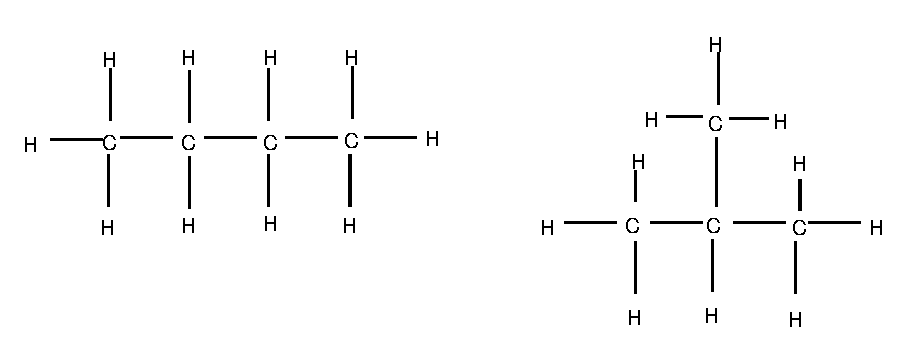
\includegraphics{../../epsimages/isomer_butane.eps}
 % isomer_butane.eps: 0x0 pixel, 300dpi, 0.00x0.00 cm, bb=5 2 427 155
\end{center}


% \begin{pspicture}(-3,-1.5)(4,3)
% %\psgrid[gridcolor=lightgray]
% \rput(-3,0){
% \rput(-1,0){\textbf{C}}
% \rput(0,0){\textbf{C}}
% \rput(1,0){\textbf{C}}
% \rput(2,0){\textbf{C}}
% \rput(-2.1,0){\textbf{H}}
% \rput(-1,1.1){\textbf{H}}
% \rput(-1,-1.1){\textbf{H}}
% \rput(0,1.1){\textbf{H}}
% \rput(0,-1.1){\textbf{H}}
% \rput(1,1.1){\textbf{H}}
% \rput(1,-1.1){\textbf{H}}
% \rput(2,1.1){\textbf{H}}
% \rput(2,-1.1){\textbf{H}}
% \rput(3,0){\textbf{H}}
% \psline(-1.3,0)(-1.7,0)
% \psline(-1,0.3)(-1,0.7)
% \psline(-1,-0.3)(-1,-0.7)
% \psline(-0.7,0)(-0.3,0)
% \psline(0,0.3)(0,0.7)
% \psline(0,-0.3)(0,-0.7)
% \psline(0.3,0)(0.7,0)
% \psline(1,0.3)(1,0.7)
% \psline(1,-0.3)(1,-0.7)
% \psline(1.3,0)(1.7,0)
% \psline(2,0.3)(2,0.7)
% \psline(2,-0.3)(2,-0.7)
% \psline(2.3,0)(2.7,0)
% \rput(6.5,0){
% \rput(-1,0){\textbf{C}}
% \rput(0,0){\textbf{C}}
% \rput(1,0){\textbf{C}}
% \rput(-2.1,0){\textbf{H}}
% \rput(-1,1.1){\textbf{H}}
% \rput(-1,-1.1){\textbf{H}}
% \rput(0,1.1){\textbf{H}}
% \rput(0,-1.1){\textbf{H}}
% \rput(1,-1.1){\textbf{H}}
% \psline(-1.3,0)(-1.7,0)
% \psline(-1,0.3)(-1,0.7)
% \psline(-1,-0.3)(-1,-0.7)
% \psline(-0.7,0)(-0.3,0)
% \psline(0,0.3)(0,0.7)
% \psline(0,-0.3)(0,-0.7)
% \psline(0.3,0)(0.7,0)
% \psline(1,0.3)(1,1.7)
% \psline(1,-0.3)(1,-0.7)
% \psline(1.3,0)(1.7,0)
% \rput(2,0){\textbf{H}}
% \rput(1,2){\textbf{C}}
% \psline(0.7,2)(0.3,2)
% \rput(0,2){\textbf{H}}
% \psline(1.3,2)(1.7,2)
% \rput(2,2){\textbf{H}}
% \psline(1,2.3)(1,2.7)
% \rput(1,3){\textbf{H}}
% }
% }
% \end{pspicture}
% \end{center}
\caption{Isomers of a 4-carbon organic compound}
\label{fig:organic:butane}
\end{figure}

If you were to count the number of carbon and hydrogen atoms in each compound, you would find that they are the same. They both have the same molecular formula (C$_{4}$H$_{10}$), but their structure is different and so are their properties. Such compounds are called \textbf{isomers}.

\Definition{Isomer}{
In chemistry, isomers are molecules with the same molecular formula and often with the same kinds of chemical bonds between atoms, but in which the atoms are arranged differently.
}

\Exercise{Isomers\\}{

Match the organic compound in Column A with its isomer Column B:\\

\begin{center}
\begin{tabular}{|c|c|}\hline
\textbf{Column A} & \textbf{Column B}\\\hline
CH$_{3}$CH(CH$_{3}$)OH & CH$_{3}$CH(CH$_{3}$)CH$_{3}$ \\\hline

\begin{pspicture}(0,-1.3)(5,1.3)
\rput(0,0){H}

\psline(0.3,0)(0.7,0)
\rput(1,0){C}
\psline(1,0.3)(1,0.7)
\rput(1,1){H}
\psline(1,-0.3)(1,-0.7)
\rput(1,-1){H}
\rput(1,0){
\psline(0.3,0)(0.7,0)
\rput(1,0){C}
\psline(1,0.3)(1,0.7)
\rput(1,1){H}
\psline(1,-0.3)(1,-0.7)
\rput(1,-1){H}
}
\rput(2,0){
\psline(0.3,0)(0.7,0)
\rput(1,0){C}
\psline(1,0.3)(1,0.7)
\rput(1,1){H}
\psline(1,-0.3)(1,-0.7)
\rput(1,-1){H}
}
\rput(3,0){
\psline(0.3,0)(0.7,0)
\rput(1,0){C}
\psline(1,0.3)(1,0.7)
\rput(1,1){H}
\psline(1,-0.3)(1,-0.7)
\rput(1,-1){H}
}
\psline(4.3,0)(4.7,0)
\rput(5,0){H}
\end{pspicture}

&

\begin{pspicture}(0,-1.3)(5,1.3)
\rput(0,0){H}

\psline(0.3,0)(0.7,0)
\rput(1,0){C}
\psline(1,0.3)(1,0.7)
\rput(1,1){H}
\psline(1,-0.3)(1,-0.7)
\rput(1,-1){H}
\rput(1,0){
\psline(0.3,0)(0.7,0)
\rput(1,0){C}
\psline(1,0.3)(1,0.7)
\rput(1,1){H}
\psline(1,-0.3)(1,-0.7)
\rput(1,-1){H}
}
\rput(2,0){
\psline(0.3,0)(0.7,0)
\rput(1,0){C}
\psline(1,0.3)(1,0.7)
\rput(1,1){CH$_{3}$}
\psline(1,-0.3)(1,-0.7)
\rput(1,-1){H}
}
\psline(3.3,0)(3.7,0)
\rput(4,0){H}
\end{pspicture}\\\hline

\begin{pspicture}(0,-1.3)(5,1.3)
\rput(0,0){H}

\psline(0.3,0)(0.7,0)
\rput(1,0){C}
\psline(1,0.3)(1,0.7)
\rput(1,1){CH$_{3}$}
\psline(1,-0.3)(1,-0.7)
\rput(1,-1){H}
\rput(1,0){
\psline(0.3,0)(0.7,0)
\rput(1,0){C}
\psline(1,0.3)(1,0.7)
\rput(1,1){H}
\psline(1,-0.3)(1,-0.7)
\rput(1,-1){H}
}
\rput(2,0){
\psline(0.3,0)(0.7,0)
\rput(1,0){C}
\psline(1,0.3)(1,0.7)
\rput(1,1){H}
\psline(1,-0.3)(1,-0.7)
\rput(1,-1){H}
}
\psline(3.3,0)(3.7,0)
\rput(4,0){H}
\end{pspicture}

& 

C$_{3}$H$_{7}$OH \\\hline

\end{tabular}
\end{center}

% Automatically inserted shortcodes - number to insert 1
\par \practiceinfo
\par \begin{tabular}[h]{cccccc}
% Question 1
(1.)	01ni	&
\end{tabular}
% Automatically inserted shortcodes - number inserted 1
}



% CHILD SECTION END 



% CHILD SECTION START 

\section{Functional groups}
\label{sec:organic:functional}

All organic compounds have a particular bond or group of atoms which we call its \textbf{functional group}. This group is important in determining how a compound will react. 

\Definition{Functional group}{
In organic chemistry, a functional group is a specific group of atoms within molecules, that are responsible for the characteristic chemical reactions of those molecules. The same functional group will undergo the same or similar chemical reaction(s) regardless of the size of the molecule it is a part of.
}

In one group of organic compounds called the \textbf{hydrocarbons}, the single, double and triple bonds of the alkanes, alkenes and alkynes are examples of functional groups. In another group, the alcohols, an oxygen and a hydrogen atom   are bonded to each other to form the functional group for those compounds (in other words an alcohol has an OH in it). All alcohols will contain an oxygen and a hydrogen atom bonded together in some part of the molecule. \\

Table \ref{fig:om:summary} summarises some of the common functional groups. We will look at these in more detail later in this chapter.

\begin{table}[!h]
\begin{center}
\begin{tabular}{|l|c|c|c|}\hline
\textbf{Name of group} & \textbf{Functional group} & \textbf{Example} & \textbf{Diagram}\\\hline
Alk\textit{ane} & 
\begin{pspicture}(-2,-1.5)(1,1.5)
%\psgrid[gridcolor=lightgray]
\rput(-1,0){C} \rput(0,0){C} \psline(-0.8,0)(-0.2,0) \psline(0.2,0)(0.8,0)
\psline(-1.2,0)(-1.8,0)
\psline(-1,0.2)(-1,0.8)
\psline(-1,-0.2)(-1,-0.8)
\psline(0,0.2)(0,0.8)
\psline(0,-0.2)(0,-0.8)
\end{pspicture}
& Ethane &
\begin{pspicture}(-2,-1.5)(1,1.5)
%\psgrid[gridcolor=lightgray]
\rput(-1,0){C}
\rput(0,0){C}
\psline(-0.8,0)(-0.2,0)
\psline(0.2,0)(0.8,0)
\psline(-1.2,0)(-1.8,0)
\psline(-1,0.2)(-1,0.8)
\psline(-1,-0.2)(-1,-0.8)
\psline(0,0.2)(0,0.8)
\psline(0,-0.2)(0,-0.8)
\rput(-2,0){H}
\rput(1,0){H}
\rput(-1,1){H}
\rput(-1,-1){H}
\rput(0,1){H}
\rput(0,-1){H}
\end{pspicture}
\\\hline

Alk\textit{ene} & 
\begin{pspicture}(-2,-1.5)(1,1.5)
%\psgrid[gridcolor=lightgray]
\rput(-1,0){\textbf{C}}

\rput(0,0){\textbf{C}}
\psline(-0.8,-0.05)(-0.2,-0.05)
\psline(-0.8,0.05)(-0.2,0.05)
\psline(0.2,0.2)(0.7,0.7)
\psline(0.2,-0.2)(0.7,-0.7)
\psline(-1.2,0.2)(-1.7,0.7)
\psline(-1.2,-0.2)(-1.7,-0.7)
\end{pspicture} & Ethene & 

\begin{pspicture}(-2,-1.5)(1,1.5)
%\psgrid[gridcolor=lightgray]
\rput(-1,0){\textbf{C}}
\rput(0,0){\textbf{C}}
\psline(-0.8,-0.05)(-0.2,-0.05)
\psline(-0.8,0.05)(-0.2,0.05)
\psline(0.2,0.2)(0.7,0.7)
\psline(0.2,-0.2)(0.7,-0.7)
\psline(-1.2,0.2)(-1.7,0.7)
\psline(-1.2,-0.2)(-1.7,-0.7)
\rput(1,1){\textbf{H}}
\rput(1,-1){\textbf{H}}
\rput(-2,1){\textbf{H}}
\rput(-2,-1){\textbf{H}}
\end{pspicture}
\\\hline

Alk\textit{yne} & 
\begin{pspicture}(-2,-1)(1,1)
%\psgrid[gridcolor=lightgray]
\rput(-1,0){\textbf{C}}
\rput(0,0){\textbf{C}}
\psline(-1.8,0)(-1.2,0)
\psline(-0.8,0.075)(-0.2,0.075)
\psline(-0.8,0)(-0.2,0)
\psline(-0.8,-0.075)(-0.2,-0.075)
\psline(0.2,0)(0.8,0)
\end{pspicture} &
Ethyne (acetylene) & 

\begin{pspicture}(-2,-1)(1,1)
%\psgrid[gridcolor=lightgray]
\rput(-2,0){\textbf{H}}
\rput(-1,0){\textbf{C}}
\rput(0,0){\textbf{C}}
\rput(1,0){\textbf{H}}
\psline(-1.8,0)(-1.2,0)
\psline(-0.8,0.075)(-0.2,0.075)
\psline(-0.8,0)(-0.2,0)
\psline(-0.8,-0.075)(-0.2,-0.075)
\psline(0.2,0)(0.8,0)
\end{pspicture}
\\\hline

Halo-alkane & 
\begin{pspicture}(-2,-2)(0,1)
\rput(-1,0){\textbf{C}}
\rput(0,0){\textbf{X}}
\rput(-1,-1.5){(X=F,Cl,Br,I)}
\psline(-1.2,0)(-1.8,0)
\psline(-0.2,0)(-0.8,0)
\psline(-1,0.2)(-1,0.8)
\psline(-1,-0.2)(-1,-0.8)
\end{pspicture} & Chloroethane & 

\begin{pspicture}(-2,-2)(0,1.5)
\rput(-1,0){\textbf{C}}
\rput(-2.2,0){\textbf{CH$_{3}$}}
\rput(0,0){\textbf{X}}
\psline(-1.2,0)(-1.8,0)
\psline(-0.2,0)(-0.8,0)
\psline(-1,0.2)(-1,0.8)
\psline(-1,-0.2)(-1,-0.8)
\rput(-1,1){\textbf{H}}
\rput(-1,-1){\textbf{H}}
\end{pspicture}\\\hline

Alcoh\textit{ol}/ alkan\textit{ol} & 
\begin{pspicture}(-2,-2)(0,1)
\rput(-1,0){\textbf{C}}
\rput(0,0){\textbf{OH}}
\psline(-1.2,0)(-1.8,0)
\psline(-0.2,0)(-0.8,0)
\psline(-1,0.2)(-1,0.8)
\psline(-1,-0.2)(-1,-0.8)
\end{pspicture} & Ethanol & 

\begin{pspicture}(0,-1.5)(3,1.5)
\rput(0,0){\textbf{H}}
\rput(1,0){\textbf{C}}
\rput(2,0){\textbf{C}}
\rput(3,0){\textbf{H}}
\rput(1,1){\textbf{H}}
\rput(1,-1){\textbf{H}}
\rput(2,1){\textbf{OH}}
\rput(2,-1){\textbf{H}}
\rput(3,0){\textbf{H}}
\psline(0.2,0)(0.8,0)
\psline(1.2,0)(1.8,0)
\psline(2.2,0)(2.8,0)
\psline(1,0.2)(1,0.8)
\psline(1,-0.2)(1,-0.8)
\psline(2,0.2)(2,0.8)
\psline(2,-0.2)(2,-0.8)
\end{pspicture}\\\hline

Carboxylic acid & 
\begin{pspicture}(-1,-1)(1,1)
\rput(0,0){\textbf{C}}
\rput(0.6,0.6){\textbf{O}}
\rput(0.6,-0.6){\textbf{OH}}
\psline(-0.2,0)(-0.8,0)
\psline(0.05,0.2)(0.5,0.5)
\psline(-0.05,0.2)(0.4,0.5)
\psline(0,-0.2)(0.6,-0.5) 
\end{pspicture} & ethanoic acid & 

\begin{pspicture}(-2,-1)(2,1.5)
\rput(-1.7,0){\textbf{CH$_{3}$}}
\psline(-1.2,0)(-0.6,0)
\rput(-0.4,0){\textbf{C}}
\rput(-0.4,1){\textbf{O}}
\psline(-0.35,0.2)(-0.35,0.8)
\psline(-0.45,0.2)(-0.45,0.8)
\psline(-0.2,0)(0.4,0)
\rput(0.8,0){\textbf{OH}}
\end{pspicture}\\\hline

Amine & 
\begin{pspicture}(-2.5,-1)(1,1.5)
\rput(-1,0){\textbf{N}}
\rput(-2,0){\textbf{R}}
\rput(0,0.8){\textbf{H}}
\rput(0,-0.8){\textbf{H}}
\psline(-1.2,0)(-1.8,0)
\psline(-0.8,0.2)(-0.2,0.6)
\psline(-0.8,-0.2)(-0.2,-0.6)
\end{pspicture} & Glycine &

\begin{pspicture}(-2.5,-2)(2.5,2)
\rput(0,0){\textbf{C}}
\rput(0,1){\textbf{H}}
\rput(0,-1){\textbf{H}}
\rput(1,0){\textbf{N}}
\rput(2,0.8){\textbf{H}}
\rput(2,-0.8){\textbf{H}}
\rput(-1,0){\textbf{C}}
\rput(-2,0.8){\textbf{O}}
\rput(-2,-0.8){\textbf{OH}}
\psline(0,0.2)(0,0.8)
\psline(0,-0.2)(0,-0.8)
\psline(-0.2,0)(-0.8,0)
\psline(-1.15,0.2)(-1.75,0.6)
\psline(-1.25,0.2)(-1.85,0.6)
\psline(-1.2,-0.2)(-1.8,-0.6)
\psline(0.2,0)(0.8,0)
\psline(1.2,0.2)(1.8,0.6)
\psline(1.2,-0.2)(1.8,-0.6)
\end{pspicture}\\\hline

\end{tabular}
\end{center}
\caption{Some functional groups of organic compounds}
\label{fig:om:summary}
\end{table}



% CHILD SECTION END 



% CHILD SECTION START 

\section{The Hydrocarbons}
\label{sec:organic:hydrocarbons}

Let us first look at a group of organic compounds known as the \textbf{hydrocarbons}. These molecules only contain carbon and hydrogen. The hydrocarbons that we are going to look at are called \textbf{aliphatic compounds}. The aliphatic compounds are divided into \textit{acyclic compounds} (chain structures) and \textit{cyclic compounds} (ring structures). The chain structures are further divided into structures that contain only \textit{single bonds} (\textbf{alkanes}), those that contain at least one \textit{double bond} (\textbf{alkenes}) and those that contain at least one \textit{triple bond} (\textbf{alkynes}). Cyclic compounds include structures such as the \textit{benzene ring}. Figure \ref{fig:om:classhydro} summarises the classification of the hydrocarbons. \\

\begin{figure}[h]
\begin{center}
\begin{pspicture}(-8,0)(8,5)
%\psgrid[gridcolor=lightgray]
\rput(0,4){Aliphatic hydrocarbons}
\psline(0,3.8)(0,3.2)
\psline(-6,3.2)(6,3.2)
\psline(-6,3.2)(-6,2.6)
\psline(6,3.2)(6,2.6)
\rput(-6,2.5){Acyclic compounds}
\rput(-6,2.2){(chain structures)}
\rput(6,2.5){Cyclic compounds}
\rput(6,2.2){(ring structures e.g. benzene ring)}
\psline(-6,2)(-6,1.4)
\psline(-7,1.4)(4,1.4)
\psline(-7,1.4)(-7,0.8)
\psline(-2,1.4)(-2,0.8)
\psline(4,1.4)(4,0.8)
\rput(-7,0.3){Alkanes (single bonds)}
\rput(-2,0.3){Alkenes (contain double bonds)}
\rput(4,0.3){Alkynes (contain triple bonds)}
\end{pspicture}
\end{center}
\caption{The classification of the aliphatic hydrocarbons}
\label{fig:om:classhydro}
\end{figure}

Hydrocarbons that contain only single bonds are called \textbf{saturated} hydrocarbons because each carbon atom is bonded to as many hydrogen atoms as possible. Figure \ref{fig:organic:saturated} shows a molecule of ethane which is a saturated hydrocarbon.\\

\begin{figure}[!h]
\begin{center}
\begin{pspicture}(-2,-1)(1,2)
%\psgrid[gridcolor=lightgray]
\rput(-1,0){C}
\rput(0,0){C}
\psline(-0.8,0)(-0.2,0)
\psline(0.2,0)(0.8,0)
\psline(-1.2,0)(-1.8,0)
\psline(-1,0.2)(-1,0.8)
\psline(-1,-0.2)(-1,-0.8)
\psline(0,0.2)(0,0.8)
\psline(0,-0.2)(0,-0.8)
\rput(-2,0){H}
\rput(1,0){H}
\rput(-1,1){H}
\rput(-1,-1){H}
\rput(0,1){H}
\rput(0,-1){H}
\end{pspicture}
\end{center}
\caption{A saturated hydrocarbon}
\label{fig:organic:saturated}
\end{figure}

Hydrocarbons that contain double or triple bonds are called \textbf{unsaturated} hydrocarbons because they don't contain as many hydrogen atoms as possible. Figure \ref{fig:organic:unsaturated} shows a molecule of ethene which is an unsaturated hydrocarbon. If you compare the number of carbon and hydrogen atoms in a molecule of ethane and a molecule of ethene, you will see that the number of hydrogen atoms in ethene is \textit{less} than the number of hydrogen atoms in ethane despite the fact that they both contain two carbon atoms. In order for an unsaturated compound to become saturated, a double bond has to be broken, and another two hydrogen atoms added for each double bond that is replaced by a single bond.

\begin{figure}[!h]
\begin{center}
\begin{pspicture}(-2,-1)(1,2)
%\psgrid[gridcolor=lightgray]
\rput(-1,0){\textbf{C}}
\rput(0,0){\textbf{C}}
\psline(-0.8,-0.05)(-0.2,-0.05)
\psline(-0.8,0.05)(-0.2,0.05)
\psline(0.2,0.2)(0.7,0.7)
\psline(0.2,-0.2)(0.7,-0.7)
\psline(-1.2,0.2)(-1.7,0.7)
\psline(-1.2,-0.2)(-1.7,-0.7)
\rput(1,1){\textbf{H}}
\rput(1,-1){\textbf{H}}
\rput(-2,1){\textbf{H}}
\rput(-2,-1){\textbf{H}}
\end{pspicture}
\end{center}
\caption{An unsaturated hydrocarbon}
\label{fig:organic:unsaturated}
\end{figure}

\begin{IFact}{
Fat that occurs naturally in living matter such as animals and plants is used as food for human consumption and contains varying proportions of saturated and unsaturated fat. Foods that contain a high proportion of saturated fat are butter, ghee, suet, tallow, lard, coconut oil, cottonseed oil, and palm kernel oil, dairy products (especially cream and cheese), meat, and some prepared foods. Diets high in saturated fat are correlated with an increased incidence of atherosclerosis and coronary heart disease according to a number of studies. Vegetable oils contain unsaturated fats and can be hardened to form margarine by adding hydrogen on to some of the carbon=carbon double bonds using a nickel catalyst. The process is called hydrogenation
}
\end{IFact}

We will now go on to look at each of the hydrocarbon groups in more detail. These groups are the alkanes, the alkenes and the alkynes.

\subsection{The Alkanes}

The alkanes are hydrocarbons that only contain \textit{single covalent bonds} between their carbon atoms. This means that they are \textit{saturated} compounds and are quite unreactive. The simplest alkane has only one carbon atom and is called \textbf{methane}. This molecule is shown in figure \ref{fig:organic:methane}.

\begin{figure}[!h]
\begin{center}
\begin{pspicture}(-3,-1)(3,1.5)
%\psgrid[gridcolor=lightgray]
\rput(-1,0){\textbf{C}}
\rput(-2,0){\textbf{H}}
\rput(0,0){\textbf{H}}
\rput(-1,1){\textbf{H}}
\rput(-1,-1){\textbf{H}}
\psline(-0.2,0)(-0.8,0)
\psline(-1.2,0)(-1.8,0)
\psline(-1,0.2)(-1,0.8)
\psline(-1,-0.2)(-1,-0.8)
\rput(-2.8,0){\textbf{(a)}}
\rput(1,0){\textbf{(b)}}
\rput(2,0){\textbf{CH$_{4}$}}
\end{pspicture}
\end{center}
\caption{The structural (a) and molecular formula (b) for methane}
\label{fig:organic:methane}
\end{figure}

The second alkane in the series has two carbon atoms and is called \textbf{ethane}. This is shown in figure \ref{fig:organic:ethane}.\\

\begin{figure}[!h]
\begin{center}
\begin{pspicture}(-3,-1)(5,1.5)
%\psgrid[gridcolor=lightgray]
\rput(-1,0){\textbf{C}}
\rput(-2,0){\textbf{H}}
\rput(-1,1){\textbf{H}}
\rput(-1,-1){\textbf{H}}
\rput(0,0){\textbf{C}}
\rput(1,0){\textbf{H}}
\rput(0,1){\textbf{H}}
\rput(0,-1){\textbf{H}}
\psline(-0.2,0)(-0.8,0)
\psline(-1.2,0)(-1.8,0)
\psline(-1,0.2)(-1,0.8)
\psline(-1,-0.2)(-1,-0.8)
\psline(0.2,0)(0.8,0)
\psline(0,0.2)(0,0.8)
\psline(0,-0.2)(0,-0.8)
\rput(-2.8,0){\textbf{(a)}}
\rput(3,0){\textbf{(b)}}
\rput(4,0){\textbf{C$_{2}$H$_{6}$}}
\end{pspicture}
\end{center}
\caption{The structural (a) and molecular formula (b) for ethane}
\label{fig:organic:ethane}
\end{figure}

The third alkane in the series has three carbon atoms and is called \textbf{propane} (Figure \ref{fig:organic:propane}).

\begin{figure}[!h]
\begin{center}
\begin{pspicture}(-3,-1)(5,1.5)
%\psgrid[gridcolor=lightgray]
\rput(-1,0){\textbf{C}}
\rput(-2,0){\textbf{H}}
\rput(-1,1){\textbf{H}}
\rput(-1,-1){\textbf{H}}
\rput(0,0){\textbf{C}}
\rput(0,1){\textbf{H}}
\rput(0,-1){\textbf{H}}
\rput(1,0){\textbf{C}}
\rput(2,0){\textbf{H}}
\rput(1,1){\textbf{H}}
\rput(1,-1){\textbf{H}}
\psline(-0.2,0)(-0.8,0)
\psline(-1.2,0)(-1.8,0)
\psline(-1,0.2)(-1,0.8)
\psline(-1,-0.2)(-1,-0.8)
\psline(0.2,0)(0.8,0)
\psline(0,0.2)(0,0.8)
\psline(0,-0.2)(0,-0.8)
\psline(1.2,0)(1.8,0)
\psline(1,0.2)(1,0.8)
\psline(1,-0.2)(1,-0.8)
\rput(-2.8,0){\textbf{(a)}}
\rput(3,0){\textbf{(b)}}
\rput(4,0){\textbf{C$_{3}$H$_{8}$}}
\end{pspicture}
\end{center}
\caption{The structural (a) and molecular formula (b) for propane}
\label{fig:organic:propane}
\end{figure}

When you look at the molecular formula for each of the alkanes, you should notice a pattern developing. For each carbon atom that is added to the molecule, two hydrogen atoms are added. In other words, each molecule differs from the one before it by CH$_{2}$. This is called a \textit{homologous series}. The alkanes have the general formula C$_{n}$H$_{2n+2}$.

The alkanes are the most important source of fuel in the world and are used extensively in the chemical industry. Some are gases (e.g. methane and ethane), while others are liquid fuels (e.g. octane, an important component of petrol).

\begin{IFact}{Some fungi use alkanes as a source of carbon and energy. One fungus \textit{Amorphotheca resinae} prefers the alkanes used in aviation fuel, and this can cause problems for aircraft in tropical areas!}
\end{IFact}

\subsection{Naming the alkanes}

In order to give compounds a name, certain rules must be followed. When naming organic compounds, the IUPAC (International Union of Pure and Applied Chemistry) nomenclature is used. We will first look at some of the steps that need to be followed when naming a compound, and then try to apply these rules to some specific examples.

\begin{enumerate}
\item{STEP 1: Recognise the \textit{functional group} in the compound. This will determine the suffix (the 'end') of the name. For example, if the compound is an alkane, the suffix will be -ane; if the compound is an alkene the suffix will be -ene; if the compound is an alcohol the suffix will be -ol, and so on.}
\item{STEP 2: Find the longest continuous carbon chain (it won't always be a \textit{straight} chain) and count the number of carbon atoms in this chain. This number will determine the prefix (the 'beginning') of the compound's name. These prefixes are shown in table \ref{tab:prefix}. So, for example, an alkane that has 3 carbon atoms will have the suffix \textit{prop} and the compound's name will be \textit{propane}.

\begin{table}[!h]
\begin{center}
\begin{tabular}{|c|c|}\hline
\textbf{Carbon atoms} & prefix \\\hline

1 & meth(ane)\\\hline
2 & eth(ane)\\\hline
3 & prop(ane)\\\hline
4 & but(ane) \\\hline
5 & pent(ane) \\\hline
6 & hex(ane) \\\hline
7 & hept(ane) \\\hline
8 & oct(ane) \\\hline
9 & non(ane) \\\hline
10 & dec(ane) \\\hline
\end{tabular}
\end{center}
\caption{The prefix of a compound's name is determined by the number of carbon atoms in the longest chain}
\label{tab:prefix}
\end{table}
}
\item{STEP 3: Number the carbons in the longest carbon chain (Important: If there is a double or triple bond, you need to start numbering so that the bond is at the carbon with the lowest number.}
\item{STEP 4: Look for any branched groups and name them. Also give them a number to show their position on the carbon chain. If there are no branched groups, this step can be left out.}
\item{STEP 5: Combine the elements of the name into a single word in the following order: branched groups; prefix; name ending according to the functional group and its position along the longest carbon chain.}
\end{enumerate}
Khan Academy video on naming simple alkanes: SIYAVULA-VIDEO:http://cnx.org/content/m39453/latest/#alkanes-1
\begin{wex}{Naming the alkanes}{Give the IUPAC name for the following compound:
\begin{figure}[H]
\begin{center}
\begin{pspicture}(-3,-1.5)(4,1.5)
%\psgrid[gridcolor=lightgray]
\rput(-1,0){\textbf{C$_{(1)}$}}
\rput(-2,0){\textbf{H}}
\rput(-1,1){\textbf{H}}
\rput(-1,-1){\textbf{H}}
\rput(0,0){\textbf{C$_{(2)}$}}
\rput(0,1){\textbf{H}}
\rput(0,-1){\textbf{H}}
\rput(1,0){\textbf{C$_{(3)}$}}
\rput(2,0){\textbf{C$_{(4)}$}}
\rput(1,1){\textbf{H}}
\rput(1,-1){\textbf{H}}
\psline(-0.2,0)(-0.8,0)
\psline(-1.2,0)(-1.8,0)
\psline(-1,0.2)(-1,0.8)
\psline(-1,-0.2)(-1,-0.8)
\psline(0.2,0)(0.8,0)
\psline(0,0.2)(0,0.8)
\psline(0,-0.2)(0,-0.8)
\psline(1.2,0)(1.8,0)
\psline(1,0.2)(1,0.8)
\psline(1,-0.2)(1,-0.8)
\rput(2,1){\textbf{H}}
\rput(2,-1){\textbf{H}}
\rput(3,0){\textbf{H}}
\psline(2.2,0)(2.8,0)
\psline(2,0.2)(2,0.8)
\psline(2,-0.2)(2,-0.8)
\end{pspicture}
\end{center}
\end{figure}
Note: The numbers attached to the carbon atoms would not normally be shown. The atoms have been numbered to help you to name the compound.
}
{\westep{Identify the functional group}
The compound is a hydrocarbon with single bonds between the carbon atoms. It is an alkane and will have a suffix of -ane.

\westep{Find the longest carbon chain}
There are four carbon atoms in the longest chain. The prefix of the compound will be 'but'.
\westep{Number the carbons in the longest chain}
In this case, it is easy. The carbons are numbered from left to right, from one to four.
\westep{Look for any branched groups, name them and give their position on the carbon chain}
There are no branched groups in this compound.
\westep{Combine the elements of the name into a single word}
The name of the compound is \textbf{butane}.
}
\end{wex}

\begin{wex}{Naming the alkanes}{Give the IUPAC name for the following compound:
\begin{figure}[H]
\begin{center}
\begin{pspicture}(-3,-3.5)(3,1.5)
%\psgrid[gridcolor=lightgray]
\rput(-1,0){\textbf{C}}
\rput(0,0){\textbf{C}}
\rput(1,0){\textbf{C}}
\rput(-2,0){\textbf{H}}
\rput(2,0){\textbf{H}}
\rput(-1,1){\textbf{H}}
\rput(-1,-1){\textbf{H}}
\rput(0,1){\textbf{H}}
\rput(1,1){\textbf{H}}
\rput(1,-1){\textbf{H}}
\rput(0,-2){\textbf{C}}
\rput(0,-3){\textbf{H}}
\rput(-1,-2){\textbf{H}}
\rput(1,-2){\textbf{H}}
\psline(-1.8,0)(-1.2,0)
\psline(-0.8,0)(-0.2,0)
\psline(0.8,0)(0.2,0)
\psline(1.8,0)(1.2,0)
\psline(-1,0.2)(-1,0.8)
\psline(-1,-0.2)(-1,-0.8)
\psline(0,0.2)(0,0.8)
\psline(0,-0.2)(0,-1.8)
\psline(1,0.2)(1,0.8)
\psline(1,-0.2)(1,-0.8)
\psline(-0.8,-2)(-0.2,-2)
\psline(0.2,-2)(0.8,-2)
\psline(0,-2.2)(0,-2.8)
\end{pspicture}
\end{center}
\end{figure}
}
{\westep{Identify the functional group}
The compound is an alkane and will have the suffix -ane.
\westep{Find the longest carbon chain}
There are three carbons in the longest chain. The prefix for this compound is -prop. 
\westep{Number the carbons in the carbon chain}
If we start at the carbon on the left, we can number the atoms as shown below:
\begin{figure}[H]
\begin{center}
\begin{pspicture}(-3,-3.5)(3,1.5)
%\psgrid[gridcolor=lightgray]
\rput(-1,0){\textbf{C$_{(1)}$}}
\rput(0,0){\textbf{C$_{(2)}$}}
\rput(1,0){\textbf{C$_{(3)}$}}
\rput(-2,0){\textbf{H}}
\rput(2,0){\textbf{H}}
\rput(-1,1){\textbf{H}}
\rput(-1,-1){\textbf{H}}
\rput(0,1){\textbf{H}}
\rput(1,1){\textbf{H}}
\rput(1,-1){\textbf{H}}
\rput(0,-2){\textbf{C}}
\rput(0,-3){\textbf{H}}
\rput(-1,-2){\textbf{H}}
\rput(1,-2){\textbf{H}}
\psline(-1.8,0)(-1.2,0)
\psline(-0.8,0)(-0.2,0)
\psline(0.8,0)(0.2,0)
\psline(1.8,0)(1.2,0)
\psline(-1,0.2)(-1,0.8)
\psline(-1,-0.2)(-1,-0.8)
\psline(0,0.2)(0,0.8)
\psline(0,-0.2)(0,-1.8)
\psline(1,0.2)(1,0.8)
\psline(1,-0.2)(1,-0.8)
\psline(-0.8,-2)(-0.2,-2)
\psline(0.2,-2)(0.8,-2)
\psline(0,-2.2)(0,-2.8)
\end{pspicture}
\end{center}
\end{figure}
\westep{Look for any branched groups, name them and give their position on the carbon chain}
There is a branched group attached to the second carbon atom. This group has the formula CH$_{3}$ which is methane. However, because it is not part of the main chain, it is given the suffix -yl (i.e. methyl). The position of the methyl group comes just before its name (see next step).
\westep{Combine the elements of the compound's name into a single word in the order of branched groups; prefix; name ending according to the functional group.}
The compound's name is \textbf{2-methylpropane}.
}
\end{wex}

\begin{wex}{Naming the alkanes}{Give the IUPAC name for the following compound:
\begin{center}
CH$_{3}$CH(CH$_{3}$)CH(CH$_{3}$)CH$_{3}$
\end{center}
(Remember that the side groups are shown in brackets after the carbon atom to which they are attached.)
}{
\westep{Draw the compound from its condensed structural formula}
The structural formula of the compound is:
\begin{figure}[H]
\begin{center}
\begin{pspicture}(-3,-0.7)(4,1)
%\psgrid[gridcolor=lightgray]
\rput(-1,0){\textbf{C$_{(1)}$}}
\rput(-2,0){\textbf{H}}
\rput(-1,1){\textbf{H}}
\rput(-1,-1){\textbf{H}}
\rput(0,0){\textbf{C$_{(2)}$}}
\rput(0,1){\textbf{CH$_{3}$}}
\rput(0,-1){\textbf{H}}
\rput(1,0){\textbf{C$_{(3)}$}}
\rput(2,0){\textbf{C$_{(4)}$}}
\rput(1,1){\textbf{CH$_{3}$}}
\rput(1,-1){\textbf{H}}
\psline(-0.2,0)(-0.8,0)
\psline(-1.2,0)(-1.8,0)
\psline(-1,0.2)(-1,0.8)
\psline(-1,-0.2)(-1,-0.8)
\psline(0.2,0)(0.8,0)
\psline(0,0.2)(0,0.8)
\psline(0,-0.2)(0,-0.8)
\psline(1.2,0)(1.8,0)
\psline(1,0.2)(1,0.8)
\psline(1,-0.2)(1,-0.8)
\rput(2,1){\textbf{H}}
\rput(2,-1){\textbf{H}}
\rput(3,0){\textbf{H}}
\psline(2.2,0)(2.8,0)
\psline(2,0.2)(2,0.8)
\psline(2,-0.2)(2,-0.8)
\end{pspicture}
\end{center}
\end{figure}
\westep{Identify the functional group}
The compound is an alkane and will have the suffix -ane.
\westep{Find the longest carbon chain}
There are four carbons in the longest chain. The prefix for this compound is -but. 
\westep{Number the carbons in the carbon chain}
If we start at the carbon on the left, carbon atoms are numbered as shown in the diagram above. A second way that the carbons could be numbered is:
\begin{figure}[H]
\begin{center}
\begin{pspicture}(-3,-0.7)(4,1)
%\psgrid[gridcolor=lightgray]
\rput(-1,0){\textbf{C$_{(1)}$}}
\rput(-2,0){\textbf{H}}
\rput(-1,1){\textbf{H}}
\rput(-1,-1){\textbf{H}}
\rput(0,0){\textbf{C$_{(2)}$}}
\rput(0,1){\textbf{CH$_{3}$}}
\rput(0,-1){\textbf{H}}
\rput(1,0){\textbf{C$_{(3)}$}}
\rput(2,0){\textbf{C}}
\rput(1,1){\textbf{CH$_{3 (4)}$}}
\rput(1,-1){\textbf{H}}
\psline(-0.2,0)(-0.8,0)
\psline(-1.2,0)(-1.8,0)
\psline(-1,0.2)(-1,0.8)
\psline(-1,-0.2)(-1,-0.8)
\psline(0.2,0)(0.8,0)
\psline(0,0.2)(0,0.8)
\psline(0,-0.2)(0,-0.8)
\psline(1.2,0)(1.8,0)
\psline(1,0.2)(1,0.8)
\psline(1,-0.2)(1,-0.8)
\rput(2,1){\textbf{H}}
\rput(2,-1){\textbf{H}}
\rput(3,0){\textbf{H}}
\psline(2.2,0)(2.8,0)
\psline(2,0.2)(2,0.8)
\psline(2,-0.2)(2,-0.8)
\end{pspicture}
\end{center}
\end{figure}
\westep{Look for any branched groups, name them and give their position on the carbon chain}
There are two methyl groups attached to the main chain. The first one is attached to the second carbon atom and the second methyl group is attached to the third carbon atom. Notice that in this example it does not matter how you have chosen to number the carbons in the main chain; the methyl groups are still attached to the second and third carbons and so the naming of the compound is not affected.
\westep{Combine the elements of the compound's name into a single word in the order of branched groups; prefix; name ending according to the functional group.}
The compound's name is \textbf{2,3-dimethyl-butane}.}
\end{wex}

\begin{wex}{Naming the alkanes}{Give the IUPAC name for the following compound:
\begin{figure}[H]
\begin{center}
\begin{pspicture}(-3,-2)(4,1)
%\psgrid[gridcolor=lightgray]
\rput(-1,0){\textbf{C}}
\rput(-2,0){\textbf{H}}
\rput(-1,1){\textbf{CH$_{3}$}}
\rput(-1,-1){\textbf{H}}
\rput(0,0){\textbf{C}}
\rput(0,1){\textbf{H}}
\rput(0,-1){\textbf{H}}
\rput(1,0){\textbf{C}}
\rput(2,0){\textbf{C}}
\rput(1,1){\textbf{H}}
\rput(1,-1){\textbf{CH$_{2}$}}
\psline(1,-1.3)(1,-1.7)
\rput(1,-2){\textbf{CH$_{3}$}}
\psline(-0.2,0)(-0.8,0)
\psline(-1.2,0)(-1.8,0)
\psline(-1,0.2)(-1,0.8)
\psline(-1,-0.2)(-1,-0.8)
\psline(0.2,0)(0.8,0)
\psline(0,0.2)(0,0.8)
\psline(0,-0.2)(0,-0.8)
\psline(1.2,0)(1.8,0)
\psline(1,0.2)(1,0.8)
\psline(1,-0.2)(1,-0.8)
\rput(2,1){\textbf{H}}
\rput(2,-1){\textbf{H}}
\rput(3,0){\textbf{H}}
\psline(2.2,0)(2.8,0)
\psline(2,0.2)(2,0.8)
\psline(2,-0.2)(2,-0.8)
\end{pspicture}
\end{center}
\end{figure}
}{\westep{Identify the functional group}
The compound is an alkane and will have the suffix -ane.

\westep{Find the longest carbon chain and number the carbons in the longest chain.}
There are six carbons in the longest chain if they are numbered as shown below. The prefix for the compound is hex-.

\begin{figure}[H]
\begin{center}
\begin{pspicture}(-3,-2)(4,1)
%\psgrid[gridcolor=lightgray]
\rput(-1,0){\textbf{C$_{(5)}$}}
\rput(-2,0){\textbf{H}}
\rput(-1,1){\textbf{CH$_{3 (6)}$}}
\rput(-1,-1){\textbf{H}}
\rput(0,0){\textbf{C$_{(4)}$}}
\rput(0,1){\textbf{H}}
\rput(0,-1){\textbf{H}}
\rput(1,0){\textbf{C$_{(3)}$}}
\rput(2,0){\textbf{C}}
\rput(1,1){\textbf{H}}
\rput(1,-1){\textbf{CH$_{2 (2)}$}}
\psline(1,-1.3)(1,-1.7)
\rput(1,-2){\textbf{CH$_{3 (1)}$}}
\psline(-0.2,0)(-0.8,0)
\psline(-1.2,0)(-1.8,0)
\psline(-1,0.2)(-1,0.8)
\psline(-1,-0.2)(-1,-0.8)
\psline(0.2,0)(0.8,0)
\psline(0,0.2)(0,0.8)
\psline(0,-0.2)(0,-0.8)
\psline(1.2,0)(1.8,0)
\psline(1,0.2)(1,0.8)
\psline(1,-0.2)(1,-0.8)
\rput(2,1){\textbf{H}}
\rput(2,-1){\textbf{H}}
\rput(3,0){\textbf{H}}
\psline(2.2,0)(2.8,0)
\psline(2,0.2)(2,0.8)
\psline(2,-0.2)(2,-0.8)
\end{pspicture}
\end{center}
\end{figure}
 \westep{Look for any branched groups, name them and give their position on the carbon chain}
There is one methyl group attached to the main chain. This is attached to the third carbon atom. 
\westep{Combine the elements of the compound's name into a single word in the order of branched groups; prefix; name ending according to the functional group.}
The compound's name is \textbf{3-methyl-hexane}.
}
\end{wex}


\Exercise{Naming the alkanes\\}{
\begin{enumerate}
\item{Give the structural formula for each of the following:}
	\begin{enumerate}
	\item{Octane}
	\item{CH$_{3}$CH$_{2}$CH$_{3}$}
	\item{CH$_{3}$CH(CH$_{3}$)CH$_{3}$}
	\item{3-ethyl-pentane}
	\end{enumerate}

\item{Give the IUPAC name for each of the following organic compounds.}
	\begin{enumerate}
	\item{\begin{pspicture}(0,-1.3)(5,1.3)
\rput(0,0){H}

\psline(0.3,0)(0.7,0)
\rput(1,0){C}
\psline(1,0.3)(1,0.7)
\rput(1,1){H}
\psline(1,-0.3)(1,-0.7)
\rput(1,-1){H}
\rput(1,0){
\psline(0.3,0)(0.7,0)
\rput(1,0){C}
\psline(1,0.3)(1,0.7)
\rput(1,1){H}
\psline(1,-0.3)(1,-0.7)
\rput(1,-1){H}
}
\rput(2,0){
\psline(0.3,0)(0.7,0)
\rput(1,0){C}
\psline(1,0.3)(1,0.7)
\rput(1,1){CH$_{3}$}
\psline(1,-0.3)(1,-0.7)
\rput(1,-1){H}
}
\psline(3.3,0)(3.7,0)
\rput(4,0){H}
\end{pspicture}
}

\item{CH$_{3}$CH$_{2}$CH(CH$_{3}$)CH$_{2}$CH$_{3}$}
\item{CH$_{3}$CH(CH$_{3}$)CH$_{2}$CH(CH$_{3}$)CH$_{3}$}
	\end{enumerate}
\end{enumerate}

% Automatically inserted shortcodes - number to insert 2
\par \practiceinfo
\par \begin{tabular}[h]{cccccc}
% Question 1
(1.)	01nj	&
% Question 2
(2.)	01nk	&
\end{tabular}
% Automatically inserted shortcodes - number inserted 2

}

\subsection{Properties of the alkanes}

We have already mentioned that the alkanes are relatively unreactive because of their stable C-C and C-H bonds. The boiling point and melting point of these molecules is determined by their molecular structure, and their surface area. The more carbon atoms there are in an alkane, the greater the surface area and therefore the higher the boiling point. The melting point also increases as the number of carbon atoms in the molecule increases. This can be seen in the data in table \ref{fig:alkane properties}.

\begin{table}[h]
\begin{center}
\begin{tabular}{|l|l|c|c|c|}\hline
\textbf{Formula} & \textbf{Name} & \textbf{Melting point ($^{0}$C)} & \textbf{Boiling point ($^{0}$C)} & \textbf{Phase at room temperature}\\\hline
CH$_{4}$ & methane & -183 & -162 & gas\\\hline
C$_{2}$H$_{6}$ & ethane & -182 & -88  & gas\\\hline
C$_{3}$H$_{8}$ & propane & -187 & -45 & gas \\\hline
C$_{4}$H$_{10}$ & butane & -138 & -0.5 & gas \\\hline
C$_{5}$H$_{12}$ & pentane & -130 & 36 & liquid \\\hline
C$_{6}$H$_{14}$ & hexane & -95 & 69 & liquid \\\hline
C$_{17}$H$_{36}$ & heptadecane & 22 & 302 & solid \\\hline
\end{tabular}
\caption{Properties of some of the alkanes}
\label{fig:alkane properties}
\end{center}
\end{table}

You will also notice that, when the molecular mass of the alkanes is low (i.e. there are few carbon atoms), the organic compounds are \textit{gases} because the intermolecular forces are weak. As the number of carbon atoms and the molecular mass increases, the compounds are more likely to be liquids or solids because the intermolecular forces are stronger.

\subsection{Reactions of the alkanes}

There are three types of reactions that can occur in saturated compounds such as the alkanes.

\begin{enumerate}
\item{\textbf{Substitution reactions}

Substitution reactions involve the removal of a hydrogen atom which is replaced by an atom of another element, such as a halogen (F, Cl, Br or I) (figure \ref{fig:organic:substitution}). The product is called a \textbf{halo-alkane}. Since alkanes are not very reactive, either heat or light is needed for this reaction to take place.\\

e.g. CH$_{2}$=CH$_{2}$ + HBr \rm${\rightarrow}$ CH$_{3}$-CH$_{2}$-Br (halo-alkane)

\begin{figure}[h]

\begin{center}
 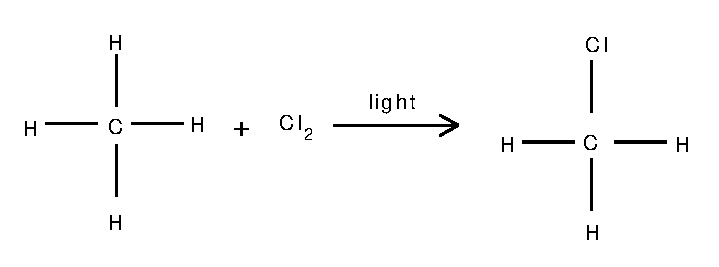
\includegraphics{../../epsimages/substitution_rxn.eps}
 % substitution_rxn.eps: 0x0 pixel, 300dpi, 0.00x0.00 cm, bb=3 6 332 118
\end{center}


% \begin{center}
% \begin{pspicture}(-2,-1)(10,1)
% \rput(-1,0){\textbf{H}}
% \psline(-0.7,0)(-0.3,0)
% \rput(0,0){\textbf{C}}
% \psline(0,0.3)(0,0.7)
% \rput(0,1){\textbf{H}}
% \psline(0.3,0.05)(0.7,0.05)
% \psline(0.3,-0.05)(0.7,-0.05)
% \rput(1,0){\textbf{C}}
% \psline(1,0.3)(1,0.7)
% \rput(1,1){\textbf{H}}
% \psline(1.3,0)(1.7,0)
% \rput(2,0){\textbf{H}}
% \rput(3,0){\textbf{+}}
% \rput(4,0){\textbf{HBr}}
% \psline[arrows=->](4.7,0)(5.5,0)
% \rput(7,0){
% \rput(-1,0){\textbf{H}}
% \psline(-0.7,0)(-0.3,0)
% \rput(0,0){\textbf{C}}
% \psline(0,0.3)(0,0.7)
% \rput(0,1){\textbf{H}}
% \psline(0.3,0)(0.7,0)
% \rput(1,0){\textbf{C}}
% \psline(1,0.3)(1,0.7)
% \rput(1,1){\textbf{H}}
% \psline(1.3,0)(1.7,0)
% \rput(2,0){\textbf{Br}}
% \rput(0,-1){\textbf{H}}
% \rput(1,-1){\textbf{H}}
% \psline(0,-0.3)(0,-0.7)
% \psline(1,-0.3)(1,-0.7)
% }
% \end{pspicture}
% \end{center}
\caption{A substitution reaction}
\label{fig:organic:substitution}
\end{figure}
}

Halo-alkanes (also sometimes called \textit{alkyl halides}) that contain methane and chlorine are substances that can be used as anaesthetics during operations. One example is trichloromethane, also known as 'chloroform' (figure \ref{fig:om:chloroform}).

\begin{figure}[h]
\begin{center}
\begin{pspicture}(-1.5,-1.5)(3,1.5)
%\psgrid[gridcolor=lightgray]
\rput(0,0){\textbf{C}}
\rput(1,1){\textbf{Cl}}
\rput(-1,1){\textbf{H}}
\rput(-1,-1){\textbf{Cl}}
\rput(1,-1){\textbf{Cl}}
\psline(0.2,0.2)(0.8,0.8)
\psline(-0.2,0.2)(-0.8,0.8)
\psline(0.2,-0.2)(0.8,-0.8)
\psline(-0.2,-0.2)(-0.8,-0.8)
\rput(2.5,0){\textbf{CHCl$_{3}$}}
\end{pspicture}

\end{center}
\caption{Trichloromethane}
\label{fig:om:chloroform}
\end{figure}


\item{\textbf{Elimination reactions}

Saturated compounds can also undergo elimination reactions to become unsaturated (figure \ref{fig:organic:elimination}). In the example below, an atom of hydrogen and chlorine are eliminated from the original compound to form an unsaturated halo-alkene.\\

e.g. \rm${ClH_{2}C-CH_{2}Cl \rightarrow H_{2}C=CHCl + HCl}$

\begin{figure}[h]
\begin{center}
\begin{pspicture}(-3,-1)(10,2)
\rput(-1,0){\textbf{H}}
\psline(-0.7,0)(-0.3,0)
\rput(0,0){\textbf{C}}
\psline(0,0.3)(0,0.7)
\rput(0,1){\textbf{H}}
\psline(0.3,0)(0.7,0)
\rput(1,0){\textbf{C}}
\psline(1,0.3)(1,0.7)
\rput(1,1){\textbf{H}}
\psline(1.3,0)(1.7,0)
\rput(2,0){\textbf{}}
\rput(0,-1){\textbf{Cl}}
\rput(1,-1){\textbf{Cl}}
\psline(0,-0.3)(0,-0.7)
\psline(1,-0.3)(1,-0.7)
\rput(2,0){\textbf{H}}
\psline[arrows=->](2.7,0)(3.5,0)
\rput(5,0){
\rput(-1,0){\textbf{H}}
\psline(-0.7,0)(-0.3,0)
\rput(0,0){\textbf{C}}
\psline(0,0.3)(0,0.7)
\rput(0,1){\textbf{H}}
\psline(0.3,0.05)(0.7,0.05)
\psline(0.3,-0.05)(0.7,-0.05)
\rput(1,0){\textbf{C}}
\psline(1,0.3)(1,0.7)
\rput(1,1){\textbf{H}}
\psline(1.3,0)(1.7,0)
\rput(2,0){\textbf{Cl}}
\rput(3,0){\textbf{+}}
\rput(4,0){\textbf{HCl}}
}
\end{pspicture}
\end{center}
\caption{An elimination reaction}
\label{fig:organic:elimination}
\end{figure}
}
\item{\textbf{Oxidation reactions}
 
When alkanes are burnt in air, they react with the oxygen in air and heat is produced. This is called an oxidation or combustion reaction. Carbon dioxide and water are given off as products. Heat is also released during the reaction. The burning of alkanes provides most of the energy that is used by man.\\

e.g. \rm${CH_{4} + 2O_{2} \rightarrow CO_{2} + 2H_{2}O + heat}$
}

\end{enumerate}


\Exercise{The Alkanes}{

\begin{enumerate}
\item{Give the IUPAC name for each of the following alkanes:}
	\begin{enumerate}
	\item{CH$_{3}$CH$_{2}$CH$_{2}$CH$_{2}$CH$_{2}$CH$_{3}$}
	\item{
	\begin{pspicture}(-3,-1.5)(2,3.5)
	%\psgrid[gridcolor=lightgray]
	\rput(-2,0){\textbf{C}}
	\rput(-2,1){\textbf{H}}
	\rput(-2,-1){\textbf{H}}
	\rput(-3,0){\textbf{H}}


	\psline(-2.8,0)(-2.2,0)
	\psline(-2,0.2)(-2,0.8)
	\psline(-2,-0.2)(-2,-0.8)
	\psline(-1.8,0)(-1.2,0)
	\rput(-1,0){\textbf{C}}
	\psline(-0.8,0)(-0.2,0)
	\rput(0,0){\textbf{C}}
	\psline(0.2,0)(0.8,0)
	\rput(1,0){\textbf{C}}
	\psline(1.2,0)(1.8,0)
	\psline(-1,0.2)(-1,1.8)
	\rput(-1,2){\textbf{C}}
	\rput(-1,3){\textbf{H}}
	\psline(-1.2,2)(-1.8,2)
	\psline(-0.2,2)(-0.8,2)
	\psline(-1,2.2)(-1,2.8)
	\rput(-2,2){\textbf{H}}
	\rput(0,2){\textbf{H}}
	\psline(-1,-0.2)(-1,-0.8)
	\rput(-1,-1){\textbf{H}}
	\rput(0,1){\textbf{H}}
	\rput(0,-1){\textbf{H}}
	\psline(0,0.2)(0,0.8)
	\psline(0,-0.2)(0,-0.8)
	\psline(1,0.2)(1,0.8)
	\rput(1,1){\textbf{H}}
	\psline(1,-0.2)(1,-0.8)
	\rput(1,-1){\textbf{H}}
	\rput(2,0){\textbf{H}}
	\end{pspicture}
	}
\item{CH$_{3}$CH$_{3}$}
\end{enumerate}

\item{Give the structural formula for each of the following compounds:}
	\begin{enumerate}
	\item{octane}
	\item{3-methyl-hexane}
	\end{enumerate}


\item{Methane is one of the simplest alkanes and yet it is an important fuel source. Methane occurs naturally in wetlands, natural gas and permafrost. However, methane can also be produced when organic wastes (e.g. animal manure and decaying material) are broken down by bacteria under conditions that are anaerobic (there is no oxygen). The simplified reaction is shown below:

\begin{center}
Organic matter \rm${\rightarrow}$ Simple organic acids \rm${\rightarrow}$ Biogas
\end{center}

The organic matter could be carbohydrates, proteins or fats which are broken down by acid-forming bacteria into simple organic acids such as acetic acid or formic acid. Methane-forming bacteria then convert these acids into biogases such as methane and ammonia.\\

The production of methane in this way is very important because methane can be used as a fuel source. One of the advantages of methane over other fuels like coal, is that it produces more energy but with lower carbon dioxide emissions. The problem however, is that methane itself is a greenhouse gas and has a much higher global warming potential than carbon dioxide. So, producing methane may in fact have an even more dangerous impact on the environment.

\begin{enumerate}
\item{What is the structural formula of methane?}
\item{Write an equation to show the reaction that takes place when methane is burned as a fuel.}
\item{Explain what is meant by the statement that methane 'has a greater global warming potential than carbon dioxide'.}
\end{enumerate}
}

\item{Chlorine and ethane react to form chloroethane and hydrogen chloride.}
	\begin{enumerate}
	\item{Write a balanced chemical equation for this reaction, using molecular formulae.}
	\item{Give the structural formula of chloroethane.}
	\item{What type of reaction has taken place in this example?}
	\end{enumerate}

\item{Petrol (C$_{8}$H$_{18}$) is in fact not pure C$_{8}$H$_{18}$ but a mixture of various \textit{alkanes}. The 'octane rating' of petrol refers to the percentage of the petrol which is C$_{8}$H$_{18}$. For example, 93 octane fuel contains 93\% C$_{8}$H$_{18}$ and 7\% other alkanes. The \textit{isomer} of C$_{8}$H$_{18}$ referred to in the 'octane rating' is in fact not octane but 2,2,4-trimethylpentane.}
	\begin{enumerate}
	\item{Write an unbalanced equation for the chemical reaction which takes place when petrol (C$_{8}$H$_{18}$) burns in excess oxygen.}
	\item{Write the general formula of the \textit{alkanes}.}
	\item{Define the term \textit{structural isomer}.}
	\item{Use the information given in this question and your knowledge of naming organic compounds to deduce and draw the full structural formula for 2,2,4-trimethylpentane.}
(IEB pg 25) 
	\end{enumerate}
\end{enumerate}

% Automatically inserted shortcodes - number to insert 5
\par \practiceinfo
\par \begin{tabular}[h]{cccccc}
% Question 1
(1.)	01nm	&
% Question 2
(2.)	01nn	&
% Question 3
(3.)	01np	&
% Question 4
(4.)	01nq	&
% Question 5
(5.)	01nr	&
\end{tabular}
% Automatically inserted shortcodes - number inserted 5

}

\subsection{The alkenes}

In the alkenes, there is at least one double bond between two carbon atoms. This means that they are \textbf{unsaturated} and are \textit{more reactive} than the alkanes. The simplest alkene is ethene (also known as ethylene), which is shown in figure \ref{fig:om:ethene3rep}.

\begin{figure}[h]
\begin{center}

\begin{pspicture}(-3,-1)(8,2)
%\psgrid[gridcolor=lightgray]
\rput(-3,0){(a)}
\rput(-1,0){\textbf{C}}
\rput(0,0){\textbf{C}}
\psline(-0.8,-0.05)(-0.2,-0.05)
\psline(-0.8,0.05)(-0.2,0.05)
\psline(0.2,0.2)(0.7,0.7)
\psline(0.2,-0.2)(0.7,-0.7)
\psline(-1.2,0.2)(-1.7,0.7)
\psline(-1.2,-0.2)(-1.7,-0.7)
\rput(1,1){\textbf{H}}
\rput(1,-1){\textbf{H}}
\rput(-2,1){\textbf{H}}
\rput(-2,-1){\textbf{H}}
\rput(2,0){(b)}
\rput(3.5,0){\textbf{CH$_{2}$CH$_{2}$}}
\rput(5,0){(c)}
\rput(6,0){\textbf{C$_{2}$H$_{4}$}}
\end{pspicture}
\end{center}
\caption{The (a) structural, (b) condensed structural and (c) molecular structure representations of ethene}
\label{fig:om:ethene3rep}
\end{figure}

As with the alkanes, the alkenes also form a homologous series. They have the general formula C$_{n}$H$_{2n}$. The second alkene in the series would therefore be C$_{3}$H$_{6}$. This molecule is known as propene (figure \ref{fig:om:propene3rep}). Note that if an alkene has two double bonds, it is called a \textbf{diene} and if it has three double bonds it is called a \textbf{triene}.

\begin{figure}[h]
\begin{center}
\begin{pspicture}(-3,-1)(8,2)
%\psgrid[gridcolor=lightgray]
\rput(-3,0){(a)}
\rput(-2,0){\textbf{H}}
\rput(-1,0){\textbf{C}}
\rput(0,0){\textbf{C}}
\rput(1,0){\textbf{C}}
\rput(-1,1){\textbf{H}}
\rput(-1,-1){\textbf{H}}
\rput(0,1){\textbf{H}}
\rput(2,1){\textbf{H}}
\rput(2,-1){\textbf{H}}
\psline(-1.8,0)(-1.2,0)
\psline(-0.8,0)(-0.2,0)
\psline(0.2,0.05)(0.8,0.05)
\psline(0.2,-0.05)(0.8,-0.05)
\psline(-1,0.2)(-1,0.8)
\psline(-1,-0.2)(-1,-0.8)
\psline(0,0.2)(0,0.8)
\psline(1.2,0.2)(1.8,0.8)
\psline(1.2,-0.2)(1.8,-.8)
\rput(4,0){\textbf{CH$_{3}$CHCH$_{2}$}}
\rput(2.5,0){(b)}
\rput(7,0){\textbf{C$_{3}$H$_{6}$}}
\rput(6,0){(c)}
\end{pspicture}
\end{center}
\caption{The (a) structural, (b) condensed structural and (c) molecular structure representations of propene}
\label{fig:om:propene3rep}
\end{figure}

The alkenes have a variety of uses. Ethylene for example is a hormone in plants that stimulates the ripening of fruits and the opening of flowers. Propene is an important compound in the petrochemicals industry. It is used as a monomer to make polypropylene and is also used as a fuel gas for other industrial processes. 

\subsection{Naming the alkenes}

Similar rules will apply in naming the alkenes, as for the alkanes. 

Khan Academy video on naming alkenes: SIYAVULA-VIDEO:http://cnx.org/content/m39453/latest/#alkenes
\begin{wex}{Naming the alkenes}{Give the IUPAC name for the following compound:

\begin{center}
\begin{pspicture}(-3,-2)(2,2)
%\psgrid[gridcolor=lightgray]
\rput(-3,0){\textbf{H}}
\psline(-2.7,0)(-2.3,0)
\rput(-2,0){\textbf{C$_{(1)}$}}
\rput(-2,1){\textbf{H}}
\rput(-2,-1){\textbf{H}}
\psline(-2,0.3)(-2,0.7)
\psline(-2,-0.3)(-2,-0.7)
\psline(-1.7,0)(-1.3,0)
\rput(-1,0){\textbf{C$_{(2)}$}}
\psline(-1,0.3)(-1,0.7)
\rput(-1,1){\textbf{H}}
\psline(-0.7,0.05)(-0.3,0.05)
\psline(-0.7,-0.05)(-0.3, -0.05)
\rput(0,0){\textbf{C$_{(3)}$}}
\rput(0,1){\textbf{H}}
\psline(0,0.3)(0,0.7)
\psline(0.3,0)(0.7,0)
\rput(1,0){\textbf{C$_{(4)}$}}
\rput(1,1){\textbf{H}}
\rput(1,-1){\textbf{H}}
\psline(1,0.3)(1,0.7)
\psline(1,-0.3)(1,-0.7)
\rput(2,0){\textbf{H}}
\psline(1.3,0)(1.7,0)
\end{pspicture}
\end{center}
}

{\westep{Identify the functional group}
The compound is an alkene and will have the suffix -ene.
\westep{Find the longest carbon chain}
There are four carbon atoms in the longest chain and so the prefix for this compound will be 'but'.
\westep{Number the carbon atoms}
Remember that when there is a double or triple bond, the carbon atoms must be numbered so that the double or triple bond is at the lowest numbered carbon. In this case, it doesn't matter whether we number the carbons from the left to right, or from the right to left. The double bond will still fall between C$_{2}$ and C$_{3}$. The position of the bond will come just before the suffix in the compound's name.
\westep{Look for any branched groups, name them and give their position on the carbon chain}
There are no branched groups in this molecule.
\westep{Name the compound}
The name of this compound is \textbf{but-2-ene}.}
\end{wex}

\begin{wex}{Naming the alkenes}{Draw the structural formula for the organic compound 3-methyl-butene\\}
{\westep{Identify the functional group}
The suffix -ene means that this compound is an alkene and there must be a double bond in the molecule. There is no number immediately before the suffix which means that the double bond must be at the first carbon in the chain.
\westep{Determine the number of carbons in the longest chain}
The prefix for the compound is 'but' so there must be four carbons in the longest chain.
\westep{Look for any branched groups}
There is a methyl group at the third carbon atom in the chain.
\westep{Combine this information to draw the structural formula for this molecule.}

\begin{figure}[H]
\begin{center}
\begin{pspicture}(-3,-1)(2.5,3.2)
%\psgrid[gridcolor=lightgray]
\rput(-2,0){\textbf{C}}
\rput(-3,0.7){\textbf{H}}
\rput(-3,-0.7){\textbf{H}}
\psline(-2.2,0.2)(-2.8,0.5)
\psline(-2.2,-0.2)(-2.8,-0.5)
\psline(-1.8,0.05)(-1.2,0.05)
\psline(-1.8,-0.05)(-1.2,-0.05)
\rput(-1,0){\textbf{C}}
\rput(-1,1){\textbf{H}}
\psline(-1,0.2)(-1,0.8)
\psline(-0.2,0)(-0.8,0)
\rput(0,0){\textbf{C}}
\psline(0,-0.2)(0,-0.8)
\rput(0,-1){\textbf{H}}
\psline(0,0.2)(0,1.8)
\rput(0,2){\textbf{C}}
\psline(-0.2,2)(-0.8,2)
\rput(-1,2){\textbf{H}}
\psline(0,2.2)(0,2.8)
\rput(0,3){\textbf{H}}
\psline(0.2,2)(0.8,2)
\rput(1,2){\textbf{H}}
\psline(0.2,0)(0.8,0)
\rput(1,0){\textbf{C}}
\psline(1,0.2)(1,0.8)
\rput(1,1){\textbf{H}}
\psline(1,-0.2)(1,-0.8)
\rput(1,-1){\textbf{H}}
\psline(1.2,0)(1.8,0)
\rput(2,0){\textbf{H}}

\end{pspicture}
\end{center}
\end{figure}
}
\end{wex}

\begin{wex}{Naming the alkenes}{Give the IUPAC name for the following compound:
\begin{center}
\begin{pspicture}(-3,-1)(2,3)
%\psgrid[gridcolor=lightgray]
\rput(-3,0){\textbf{H}}
\psline(-2.7,0)(-2.3,0)
\rput(-2,0){\textbf{C$_{(1)}$}}
\rput(-2,1){\textbf{H}}
\psline(-2,0.3)(-2,0.7)
\psline(-1.7,0.05)(-1.3,0.05)
\psline(-1.7,-0.05)(-1.3,-0.05)
\rput(-1,0){\textbf{C$_{(2)}$}}
\psline(-1,0.3)(-1,0.7)
\rput(-1,1){\textbf{CH$_{2}$}}
\psline(-1,1.3)(-1,1.7)
\rput(-1,2){\textbf{CH$_{3}$}}
\psline(-0.7,0)(-0.3,0)
\rput(0,0){\textbf{C$_{(3)}$}}
\rput(0,1){\textbf{H}}
\psline(0,0.3)(0,0.7)
\psline(0.3,0.05)(0.7,0.05)
\psline(0.3,-0.05)(0.7,-0.05)
\rput(1,0){\textbf{C$_{(4)}$}}
\rput(1,1){\textbf{H}}
\psline(1,0.3)(1,0.7)
\rput(2,0){\textbf{H}}
\psline(1.3,0)(1.7,0)
\end{pspicture}
\end{center}
}

{\westep{Identify the functional group}
The compound is an alkene and will have the suffix -ene. There is a double bond between the first and second carbons and also between the third and forth carbons. The organic compound is therefore a 'diene'.
\westep{Find the longest carbon chain and number the carbon atoms}
There are four carbon atoms in the longest chain and so the prefix for this compound will be 'but'. The carbon atoms are numbered 1 to 4 in the diagram above. Remember that the main carbon chain must contain both the double bonds.
\westep{Look for any branched groups, name them and give their position on the carbon chain}
There is an ethyl group on the second carbon.
\westep{Name the compound}
The name of this compound is \textbf{2-ethyl-but-1,3-diene}.}
\end{wex}



\Exercise{Naming the alkenes\\}{
Give the IUPAC name for each of the following alkenes:

\begin{enumerate}
\item{CH$_{2}$CHCH$_{2}$CH$_{2}$CH$_{3}$}
\item{CH$_{3}$CHCHCH$_{3}$}
\item{}

\begin{pspicture}(0,-1.3)(4,1.3)
\rput(0,0){H}
\psline(0.3,0)(0.7,0)

\rput(1,0){C}
\psline(1,0.3)(1,0.7)
\rput(1,1){H}
\psline(1.3,0.05)(1.7,0.05)
\psline(1.3,-0.05)(1.7,-0.05)
\rput(1,0){
\rput(1,0){C}
\psline(1.3,0.05)(1.7,0.05)
\psline(1.3,-0.05)(1.7,-0.05)
}
\rput(2,0){
\rput(1,0){C}
\psline(1,0.3)(1,0.7)
\rput(1,1){H}
\psline(1.3,0)(1.7,0)
}
\rput(3,0){
\rput(1,0){C}
\psline(1,0.3)(1,0.7)
\rput(1,1){H}
\psline(1,-0.3)(1,-0.7)
\rput(1,-1){H}
\psline(1.3,0)(1.7,0)
}
\rput(5,0){H}
\end{pspicture}

\end{enumerate}

% Automatically inserted shortcodes - number to insert 3
\par \practiceinfo
\par \begin{tabular}[h]{cccccc}
% Question 1
(1.)	01ns	&
% Question 2
(2.)	01nt	&
% Question 3
(3.)	01nu	&
\end{tabular}
% Automatically inserted shortcodes - number inserted 3
}

\subsection{The properties of the alkenes}

The properties of the alkenes are very similar to those of the alkanes, except that the alkenes are more reactive because they are unsaturated. As with the alkanes, compounds that have four or less carbon atoms are gases at room temperature, while those with five or more carbon atoms are liquids.

\subsection{Reactions of the alkenes}

Alkenes can undergo \textbf{addition reactions} because they are unsaturated. They readily react with hydrogen, water and the halogens. The double bond is broken and a single, saturated bond is formed. A new group is then added to one or both of the carbon atoms that previously made up the double bond. The following are some examples:

\begin{enumerate}
\item{\textbf{Hydrogenation reactions} 

A catalyst such as platinum is normally needed for these reactions

\rm${H_{2}C=CH_{2} + H_{2} \rightarrow H_{3}C-CH_{3}}$ (figure \ref{fig:organic:hydrogenation})

\begin{figure}[h]
\begin{center}
\begin{pspicture}(-2,-0.5)(10,1.5)
\rput(-1,0){\textbf{H}}
\psline(-0.7,0)(-0.3,0)
\rput(0,0){\textbf{C}}
\psline(0,0.3)(0,0.7)
\rput(0,1){\textbf{H}}
\psline(0.3,0.05)(0.7,0.05)
\psline(0.3,-0.05)(0.7,-0.05)
\rput(1,0){\textbf{C}}
\psline(1,0.3)(1,0.7)
\rput(1,1){\textbf{H}}
\psline(1.3,0)(1.7,0)
\rput(2,0){\textbf{H}}
\rput(3,0){\textbf{+}}
\rput(4,0){\textbf{H$_{2}$}}
\psline[arrows=->](4.7,0)(5.5,0)
\rput(7,0){
\rput(-1,0){\textbf{H}}
\psline(-0.7,0)(-0.3,0)
\rput(0,0){\textbf{C}}
\psline(0,0.3)(0,0.7)
\rput(0,1){\textbf{H}}
\psline(0.3,0)(0.7,0)
\rput(1,0){\textbf{C}}
\psline(1,0.3)(1,0.7)
\rput(1,1){\textbf{H}}
\psline(1.3,0)(1.7,0)
\rput(2,0){\textbf{H}}
\rput(0,-1){\textbf{H}}
\rput(1,-1){\textbf{H}}
\psline(0,-0.3)(0,-0.7)
\psline(1,-0.3)(1,-0.7)
}
\end{pspicture}
\end{center}
\caption{A hydrogenation reaction}
\label{fig:organic:hydrogenation}
\end{figure}
}

\item{\textbf{Halogenation reactions}

\rm${CH_{2}=CH_{2} + HBr \rightarrow CH_{3}-CH_{2}-Br}$ (figure \ref{fig:organic:halogenation})

\begin{figure}[h]
\begin{center}
\begin{pspicture}(-2,-1)(10,1.5)
\rput(-1,0){\textbf{H}}
\psline(-0.7,0)(-0.3,0)
\rput(0,0){\textbf{C}}
\psline(0,0.3)(0,0.7)
\rput(0,1){\textbf{H}}
\psline(0.3,0.05)(0.7,0.05)
\psline(0.3,-0.05)(0.7,-0.05)
\rput(1,0){\textbf{C}}
\psline(1,0.3)(1,0.7)
\rput(1,1){\textbf{H}}
\psline(1.3,0)(1.7,0)
\rput(2,0){\textbf{H}}
\rput(3,0){\textbf{+}}
\rput(4,0){\textbf{HBr}}
\psline[arrows=->](4.7,0)(5.5,0)
\rput(7,0){
\rput(-1,0){\textbf{H}}
\psline(-0.7,0)(-0.3,0)
\rput(0,0){\textbf{C}}
\psline(0,0.3)(0,0.7)
\rput(0,1){\textbf{H}}
\psline(0.3,0)(0.7,0)
\rput(1,0){\textbf{C}}
\psline(1,0.3)(1,0.7)
\rput(1,1){\textbf{H}}
\psline(1.3,0)(1.7,0)
\rput(2,0){\textbf{Br}}
\rput(0,-1){\textbf{H}}
\rput(1,-1){\textbf{H}}
\psline(0,-0.3)(0,-0.7)
\psline(1,-0.3)(1,-0.7)
}
\end{pspicture}
\end{center}
\caption{A halogenation reaction}
\label{fig:organic:halogenation}
\end{figure}
}

\item{\textbf{The formation of alcohols}

\rm${CH_{2}=CH_{2} + H_{2}O \rightarrow CH_{3}-CH_{2}-OH}$ (figure \ref{fig:organic:forming alcohols})

\begin{figure}[h]
\begin{center}
\begin{pspicture}(-2,-1)(10,1.5)
\rput(-1,0){\textbf{H}}
\psline(-0.7,0)(-0.3,0)
\rput(0,0){\textbf{C}}
\psline(0,0.3)(0,0.7)
\rput(0,1){\textbf{H}}
\psline(0.3,0.05)(0.7,0.05)
\psline(0.3,-0.05)(0.7,-0.05)
\rput(1,0){\textbf{C}}
\psline(1,0.3)(1,0.7)
\rput(1,1){\textbf{H}}
\psline(1.3,0)(1.7,0)
\rput(2,0){\textbf{H}}
\rput(3,0){\textbf{+}}
\rput(4,0){\textbf{H$_{2}$O}}
\psline[arrows=->](4.7,0)(5.5,0)
\rput(7,0){
\rput(-1,0){\textbf{H}}
\psline(-0.7,0)(-0.3,0)
\rput(0,0){\textbf{C}}
\psline(0,0.3)(0,0.7)
\rput(0,1){\textbf{H}}
\psline(0.3,0)(0.7,0)
\rput(1,0){\textbf{C}}
\psline(1,0.3)(1,0.7)
\rput(1,1){\textbf{H}}
\psline(1.3,0)(1.7,0)
\rput(2,0){\textbf{OH}}
\rput(0,-1){\textbf{H}}
\rput(1,-1){\textbf{H}}
\psline(0,-0.3)(0,-0.7)
\psline(1,-0.3)(1,-0.7)
}
\end{pspicture}
\end{center}
\caption{The formation of an alcohol}
\label{fig:organic:forming alcohols}
\end{figure}
}
\end{enumerate}

\Exercise{The Alkenes\\}{
\begin{enumerate}
\item{Give the IUPAC name for each of the following organic compounds:}
	\begin{enumerate}
	\item{
\begin{pspicture}(-3,-3)(2,2)
	%\psgrid[gridcolor=lightgray]
	\rput(-2,0){\textbf{C}}
	\rput(-2,1){\textbf{H}}
	\rput(-2,-1){\textbf{H}}
	\rput(-3,0){\textbf{H}}
	\psline(-2.8,0)(-2.2,0)
	\psline(-2,0.2)(-2,0.8)
	\psline(-2,-0.2)(-2,-0.8)
	\psline(-1.8,0)(-1.2,0)
	\rput(-1,0){\textbf{C}}
	\psline(-0.8,0.05)(-0.2,0.05)
	\psline(-0.8,-0.05)(-0.2,-0.05)
	\rput(0,0){\textbf{C}}
	\psline(0.2,0)(0.8,0)
	\rput(1,0){\textbf{C}}
	\psline(1.2,0)(1.8,0)
	\psline(-1,-0.2)(-1,-0.8)
	\rput(-1,-1){\textbf{H}}
	\rput(0,-1){\textbf{H}}
	\psline(0,-0.2)(0,-0.8)
	\psline(1,0.2)(1,0.8)
	\rput(1,1){\textbf{H}}
	\psline(1,-0.2)(1,-1.8)
	\rput(1,-2){\textbf{C}}
	\rput(1,-3){\textbf{H}}
	\rput(0,-2){\textbf{H}}
	\rput(2,-2){\textbf{H}}
	\psline(0.8,-2)(0.2,-2)
	\psline(1.8,-2)(1.2,-2)
	\psline(1,-2.2)(1,-2.8)
	\rput(2,0){\textbf{H}}
	\end{pspicture}
	}
	\item{CH$_{3}$CHCH$_{2}$}
	\end{enumerate}

\item{Refer to the data table below which shows the melting point and boiling point for a number of different organic compounds.

\begin{center}
\begin{tabular}{|l|l|c|c|}\hline
\textbf{Formula} & \textbf{Name} & \textbf{Melting point ($^{0}$C)} & \textbf{Boiling point ($^{0}$C)}\\\hline
C$_{4}$H$_{10}$ & Butane & -138 & -0.5 \\\hline
C$_{5}$H$_{12}$ & Pentane & -130 & 36 \\\hline
C$_{6}$H$_{14}$ & Hexane & -95 & 69 \\\hline
C$_{4}$H$_{8}$ & Butene & -185 & -6 \\\hline
C$_{5}$H$_{10}$ & Pentene & -138 & 30 \\\hline
C$_{6}$H$_{12}$ & Hexene & -140 & 63 \\\hline
\end{tabular}
\end{center}
	\begin{enumerate}
	\item{At room temperature (approx. 25$^{0}$C), which of the organic compounds in the table are:
		\begin{enumerate}
		\item{gases}
		\item{liquids}
		\end{enumerate}
}
	\item{In the alkanes...
		\begin{enumerate}
		\item{Describe what happens to the melting point and boiling point as the number of carbon atoms in the compound increases.}
		\item{Explain why this is the case.}
		\end{enumerate}
}
	\item{If you look at an alkane and an alkene that have the same number of carbon atoms...
		\begin{enumerate}
		\item{How do their melting points and boiling points compare?}
		\item{Can you explain why their melting points and boiling points are different?}
		\end{enumerate}
}
	\item{Which of the compounds, hexane or hexene, is more reactive? Explain your answer.}
	\end{enumerate}
}

\item{
The following reaction takes place:\\
\begin{center}
\rm${CH_{3}CHCH_{2} + H_{2} \rightarrow CH_{3}CH_{2}CH_{3}}$
\end{center}

\begin{enumerate}
\item{Give the name of the organic compound in the reactants.}
\item{What is the name of the product?}
\item{What type of reaction is this?}
\item{Which compound in the reaction is a saturated hydrocarbon?}
\end{enumerate}

}
\end{enumerate}
% Automatically inserted shortcodes - number to insert 3
\par \practiceinfo
\par \begin{tabular}[h]{cccccc}
% Question 1
(1.)	01nv	&
% Question 2
(2.)	01nw	&
% Question 3
(3.)	01nx	&
\end{tabular}
% Automatically inserted shortcodes - number inserted 3

}


\subsection{The Alkynes}

In the alkynes, there is at least one triple bond between two of the carbon atoms. They are unsaturated compounds and are therefore highly reactive. Their general formula is C$_{n}$H$_{2n-2}$. The simplest alkyne is ethyne (figure \ref{fig:om:ethyne}), also known as acetylene. Many of the alkynes are used to synthesise other chemical products.

\begin{figure}[h]
\begin{center}


\begin{pspicture}(-2,-0.5)(1,0.5)
%\psgrid[gridcolor=lightgray]
\rput(-2,0){\textbf{H}}
\rput(-1,0){\textbf{C}}
\rput(0,0){\textbf{C}}
\rput(1,0){\textbf{H}}
\psline(-1.8,0)(-1.2,0)
\psline(-0.8,0.075)(-0.2,0.075)
\psline(-0.8,0)(-0.2,0)
\psline(-0.8,-0.075)(-0.2,-0.075)
\psline(0.2,0)(0.8,0)
\end{pspicture}
\end{center}
\caption{Ethyne (acetylene)}
\label{fig:om:ethyne}
\end{figure}

\begin{IFact}{
The raw materials that are needed to make acetylene are calcium carbonate and coal. Acetylene can be produced through the following reactions:
\begin{center}
\rm${CaCO_{3} \rightarrow CaO}$

\rm${CaO + 3C \rightarrow CaC_{2} + CO}$

\rm${CaC_{2} + 2H_{2}O \rightarrow Ca(OH)_{2} + C_{2}H_{2}}$
\end{center}

An important use of acetylene is in oxyacetylene gas welding. The fuel gas burns with oxygen in a torch. An incredibly high heat is produced, and this is enough to melt metal.
}
\end{IFact}

\subsection{Naming the alkynes}

The same rules will apply as for the alkanes and alkenes, except that the suffix of the name will now be -yne.

\begin{wex}{Naming the alkynes}{Give the IUPAC name for the following compound:

\begin{figure}[H]
\begin{center}
\begin{pspicture}(-4,-1.5)(4,1)
%\psgrid[gridcolor=lightgray]
\rput(-3,0){\textbf{CH$_{3}$}}
\rput(-2,0){\textbf{CH}}
\psline(-2.6,0)(-2.4,0)
\rput(-1,0){\textbf{CH$_{2}$}}
\psline(-1.6,0)(-1.4,0)
\rput(-2,-1){\textbf{CH$_{3}$}}
\psline(-2,-0.3)(-2,-0.7)
\rput(0,0){\textbf{C}}
\psline(0.4,0)(0.6,0)
\rput(1,0){\textbf{C}}
\rput(2,0){\textbf{CH$_{3}$}}
\psline(0.4,0.075)(0.6,0.075)
\psline(0.4,0)(0.6,0)
\psline(0.4,-0.075)(0.6,-0.075)
\psline(1.4,0)(1.6,0)
\psline(-0.6,0)(-0.4,0)
\end{pspicture}
\end{center}
\end{figure}
}
{\westep{Identify the functional group}
There is a triple bond between two of the carbon atoms, so this compound is an alkyne. The suffix will be -yne. The triple bond is at the second carbon, so the suffix will in fact be 2-yne.\\
\westep{Find the longest carbon chain and give the compound the correct prefix}
If we count the carbons in a straight line, there are six. The prefix of the compound's name will be 'hex'.
\westep{Number the carbons in the longest chain}
In this example, you will need to number the carbons from right to left so that the triple bond is between carbon atoms with the lowest numbers.
\westep{Look for any branched groups, name them and show the number of the carbon atom to which the group is attached}
There is a methyl (CH$_{3}$) group attached to the fifth carbon (remember we have numbered the carbon atoms from right to left).
\westep{Combine the elements of the name into a single word in the following order: branched groups; prefix; name ending according to the functional group and its position along the longest carbon chain.}
If we follow this order, the name of the compound is \textbf{5-methyl-hex-2-yne}.
}
\end{wex}

\Exercise{The alkynes\\}{

Give the IUPAC name for each of the following organic compounds.

\begin{enumerate}
\item{
\begin{pspicture}(-3,-1.5)(3,1.5)
\rput(-3,0){\textbf{H}}
\psline(-2.7,0)(-2.3,0)
\rput(-2,0){\textbf{C}}
\psline(-2,0.3)(-2,0.7)
\rput(-2,1){\textbf{H}}
\psline(-2,-0.3)(-2,-0.7)
\rput(-2,-1){\textbf{H}}
\psline(-1.7,0)(-1.3,0)
\rput(-1,0){\textbf{C}}
\psline(-1,0.3)(-1,0.7)
\rput(-1,1){\textbf{CH$_{3}$}}
\psline(-1,-0.3)(-1,-0.7)
\rput(-1,-1){\textbf{H}}
\psline(-0.7,0)(-0.3,0)
\rput(0,0){\textbf{C}}
\psline(0.3,0.05)(0.7,0.05)
\psline(0.3,0)(0.7,0)
\psline(0.3,-0.05)(0.7,-0.05)
\rput(1,0){\textbf{C}}
\psline(1.3,0)(1.7,0)
\rput(2,0){\textbf{H}}
\end{pspicture}
}

\item{
C$_{2}$H$_{2}$
}

\item{
CH$_{3}$CH$_{2}$CCH
}
\end{enumerate}
% Automatically inserted shortcodes - number to insert 3
\par \practiceinfo
\par \begin{tabular}[h]{cccccc}
% Question 1
(1.)	01ny	&
% Question 2
(2.)	01nz	&
% Question 3
(3.)	01p0	&
\end{tabular}
% Automatically inserted shortcodes - number inserted 3
}



% CHILD SECTION END 



% CHILD SECTION START 

\section{The Alcohols}

An alcohol is any organic compound where there is a \textit{hydroxyl} functional group (-OH) bound to a carbon atom. The general formula for a simple alcohol is C$_{n}$H$_{2n+1}$OH.\\

The simplest and most commonly used alcohols are methanol and ethanol (figure \ref{fig:om:metheth}).
\begin{figure}[h]
\begin{center}
\begin{pspicture}(-4,-1.5)(4,1.5)
%\psgrid[gridcolor=lightgray]
\rput(-2,0){\textbf{C}}
\rput(-3,0){\textbf{H}}
\rput(-1,0){\textbf{H}}
\rput(-2,1){\textbf{OH}}
\rput(-2,-1){\textbf{H}}
\psline(-2.8,0)(-2.2,0)
\psline(-1.8,0)(-1.2,0)
\psline(-2,0.2)(-2,0.8)
\psline(-2,-0.2)(-2,-0.8)
\rput(-3.5,1){\textbf{(a)}}

\rput(0,0){\textbf{H}}
\rput(1,0){\textbf{C}}
\rput(2,0){\textbf{C}}
\rput(3,0){\textbf{H}}
\rput(1,1){\textbf{H}}
\rput(1,-1){\textbf{H}}
\rput(2,1){\textbf{OH}}
\rput(2,-1){\textbf{H}}
\rput(3,0){\textbf{H}}
\psline(0.2,0)(0.8,0)
\psline(1.2,0)(1.8,0)
\psline(2.2,0)(2.8,0)
\psline(1,0.2)(1,0.8)
\psline(1,-0.2)(1,-0.8)
\psline(2,0.2)(2,0.8)
\psline(2,-0.2)(2,-0.8)
\rput(0,1){\textbf{(b)}}
\end{pspicture}
\end{center}
\caption{(a) methanol and (b) ethanol}
\label{fig:om:metheth}
\end{figure}

The alcohols have a number of different uses:

\begin{itemize}
\item{methylated spirits (surgical spirits) is a form of ethanol where methanol has been added}
\item{ethanol is used in alcoholic drinks}
\item{ethanol is used as an industrial solvent}
\item{methanol and ethanol can both be used as a fuel and they burn more cleanly than gasoline or diesel (refer to Grade 11 for more information on biofuels as an alternative energy resource.)}
\item{ethanol is used as a solvent in medical drugs, perfumes and vegetable essences}
\item{ethanol is an antiseptic}
\end{itemize}

\begin{IFact}

'Fermentation' refers to the conversion of sugar to alcohol using yeast (a fungus). The process of fermentation produces items such as wine, beer and yoghurt. To make wine, grape juice is fermented to produce alcohol. This reaction is shown below:
\begin{center}
\rm${C_{6}H_{12}O_{6} \rightarrow 2CO_{2} + 2C_{2}H_{5}OH + energy}$
\end{center}
\end{IFact}

\begin{IFact}{
Ethanol is a diuretic. In humans, ethanol reduces the secretion of a hormone called antidiuretic hormone (ADH). The role of ADH is to control the amount of water that the body retains. When this hormone is not secreted in the right quantities, it can cause dehyration because too much water is lost from the body in the urine. This is why people who drink too much alcohol can become dehydrated, and experience symptoms such as headaches, dry mouth, and lethargy. Part of the reason for the headaches is that dehydration causes the brain to shrink away from the skull slightly. The effects of drinking too much alcohol can be reduced by drinking lots of water.}
\end{IFact}

\subsection{Naming the alcohols}
\label{subsec:om:alcoholnaming}

The rules used to name the alcohols are similar to those already discussed for the other compounds, except that the suffix of the name will be different because the compound is an alcohol.
Khan Academy video on alcohols: SIYAVULA-VIDEO:http://cnx.org/content/m39455/latest/#alcohols
\begin{wex}{Naming alcohols 1}{Give the IUPAC name for the following organic compound

\begin{figure}[H]
\begin{center}
\begin{pspicture}(-3,-1.5)(3,1.5)
%\psgrid[gridcolor=lightgray]
\rput(-2,0){\textbf{H}}
\psline(-1.8,0)(-1.2,0)
\rput(-1,0){\textbf{C$_{1}$}}
\psline(-1,0.2)(-1,0.8)
\rput(-1,1){\textbf{H}}
\psline(-1,-0.2)(-1,-0.8)
\rput(-1,-1){\textbf{H}}
\psline(-0.2,0)(-0.8,0)
\rput(0,0){\textbf{C$_{2}$}}
\psline(0,0.2)(0,0.8)
\rput(0,1){\textbf{OH}}
\psline(0,-0.2)(0,-0.8)
\rput(0,-1){\textbf{H}}
\psline(0.2,0)(0.8,0)
\rput(1,0){\textbf{C$_{3}$}}
\psline(1,0.2)(1,0.8)
\rput(1,1){\textbf{H}}
\psline(1,-0.2)(1,-0.8)
\rput(1,-1){\textbf{H}}
\psline(1.2,0)(1.8,0)
\rput(2,0){\textbf{H}}
\end{pspicture}
\end{center}
\end{figure}
}
{\westep{Identify the functional group}
The compound has an -OH (hydroxyl) functional group and is therefore an alcohol. The compound will have the suffix -ol.\westep{Find the longest carbon chain}
There are three carbons in the longest chain. The prefix for this compound will be 'prop'. Since there are only single bonds between the carbon atoms, the suffix becomes 'propan' (similar to the alkane 'propane').
\westep{Number the carbons in the carbon chain}
In this case, it doesn't matter whether you start numbering from the left or right. The hydroxyl group will still be attached to the middle carbon atom, numbered '2'.
\westep{Look for any branched groups, name them and give their position on the carbon chain.}
There are no branched groups in this compound, but you still need to indicate the position of the hydroxyl group on the second carbon. The suffix will be -2-ol because the hydroxyl group is attached to the second carbon.
\westep{Combine the elements of the compound's name into a single word in the order of branched groups; prefix; name ending according to the functional group.}
The compound's name is propan-2-ol.
}
\end{wex}

\begin{wex}{Naming alcohols 2}{Give the IUPAC name for the following compound:

\begin{figure}[H]
\begin{center}
\begin{pspicture}(-3,-2)(3,2)
%\psgrid[gridcolor=lightgray]
\rput(-2,0){\textbf{H}}
\psline(-1.8,0)(-1.2,0)
\rput(-1,0){\textbf{C$_{1}$}}
\psline(-1,0.2)(-1,0.8)
\rput(-1,1){\textbf{OH}}
\psline(-1,-0.2)(-1,-0.8)
\rput(-1,-1){\textbf{H}}
\psline(-0.2,0)(-0.8,0)
\rput(0,0){\textbf{C$_{2}$}}
\psline(0,0.2)(0,0.8)
\rput(0,1){\textbf{OH}}
\psline(0,-0.2)(0,-0.8)
\rput(0,-1){\textbf{H}}
\psline(0.2,0)(0.8,0)
\rput(1,0){\textbf{C$_{3}$}}
\psline(1,0.2)(1,0.8)
\rput(1,1){\textbf{H}}
\psline(1,-0.2)(1,-0.8)
\rput(1,-1){\textbf{H}}
\psline(1.2,0)(1.8,0)
\rput(2,0){\textbf{C$_{4}$}}
\psline(2,0.2)(2,0.8)
\rput(2,1){\textbf{H}}
\psline(2,-0.2)(2,-0.8)
\rput(2,-1){\textbf{H}}
\psline(2.2,0)(2.8,0)
\rput(3,0){\textbf{H}}
\end{pspicture}
\end{center}
\end{figure}
}
{\westep{Identify the functional group}
The compound has an -OH (hydroxyl) functional group and is therefore an alcohol. There are \textit{two} hydroxyl groups in the compound, so the suffix will be -diol.
\westep{Find the longest carbon chain}
There are four carbons in the longest chain. The prefix for this compound will be 'butan'. 
\westep{Number the carbons in the carbon chain}
The carbons will be numbered from left to right so that the two hydroxyl groups are attached to carbon atoms with the lowest numbers.
\westep{Look for any branched groups, name them and give their position on the carbon chain.}
There are no branched groups in this compound, but you still need to indicate the position of the hydroxyl groups on the first and second carbon atoms. The suffix will therefore become 1,2-diol.
\westep{Combine the elements of the compound's name into a single word in the order of branched groups; prefix; name ending according to the functional group.}
The compound's name is butan-1,2-diol.
}
\end{wex}
 
\Exercise{Naming the alcohols\\}{
\begin{enumerate}
\item{Give the structural formula of each of the following organic compounds:}
	\begin{enumerate}
	\item{pentan-3-ol}
	\item{butan-2,3-diol}
	\item{2-methyl-propanol}
	\end{enumerate}
\item{Give the IUPAC name for each of the following:}
	\begin{enumerate}
	\item{CH$_{3}$CH$_{2}$CH(OH)CH$_{3}$}
	\item{
\begin{pspicture}(0,-1.3)(5,1.3)
\rput(0,0){CH$_{3}$}
\psline(0.3,0)(0.7,0)
\rput(1,0){C}
\psline(1,0.3)(1,0.7)
\rput(1,1){H}
\psline(1,-0.3)(1,-0.7)
\rput(1,-1){OH}
\psline(1.3,0)(1.7,0)
\rput(2,0){CH$_{2}$}
\psline(2.3,0)(2.7,0)
\rput(3,0){CH$_{2}$}
\psline(3.3,0)(3.7,0)
\rput(4,0){CH$_{3}$}
\end{pspicture}
}
	\end{enumerate}
\end{enumerate}
% Automatically inserted shortcodes - number to insert 2
\par \practiceinfo
\par \begin{tabular}[h]{cccccc}
% Question 1
(1.)	01p1	&
% Question 2
(2.)	01p2	&
\end{tabular}
% Automatically inserted shortcodes - number inserted 2
}

\subsection{Physical and chemical properties of the alcohols}
\label{sec:om:physchem}

The hydroxyl group affects the \textbf{solubility} of the alcohols. The hydroxyl group generally makes the alcohol molecule \textit{polar} and therefore more likely to be \textbf{soluble} in water. However, the carbon chain resists solubility, so there are two opposing trends in the alcohols. Alcohols with shorter carbon chains are usually more soluble than those with longer carbon chains.\\

Alcohols tend to have higher \textbf{boiling points} than the hydrocarbons because of the strong hydrogen bond between hydrogen and oxygen atoms. \\

Alcohols can show either \textbf{acidic} or \textbf{basic} properties because of the hydroxyl group. They also undergo oxidation reactions to form aldehydes, ketones and carboxylic acids.


\Activity{Case Study}{The uses of the alcohols}{Read the extract below and then answer the questions that follow:\\

The alcohols are a very important group of organic compounds, and they have a variety of uses. Our most common use of the word 'alcohol' is with reference to alcoholic drinks. The alcohol in drinks is in fact \textbf{ethanol}. But ethanol has many more uses apart from alcoholic drinks! When ethanol burns in air, it produces carbon dioxide, water and energy and can therefore be used as a fuel on its own, or in mixtures with petrol. Because ethanol can be produced through fermentation, this is a useful way for countries without an oil industry to reduce imports of petrol. Ethanol is also used as a solvent in many perfumes and cosmetics.\\

\textbf{Methanol} can also be used as a fuel, or as a petrol additive to improve combustion. Most methanol is used as an industrial feedstock, in other words it is used to make other things such as methanal (formaldehyde), ethanoic acid and methyl esters. In most cases, these are then turned into other products.\\

\textbf{Propan-2-ol} is another important alcohol, which is used in a variety of applications as a solvent.\\

\textbf{Questions}

\begin{enumerate}
\item{Give the structural formula for propan-2-ol.}
\item{Write a balanced chemical equation for the combustion reaction of ethanol.}
\item{Explain why the alcohols are good solvents.}
\end{enumerate}
}



% CHILD SECTION END 



% CHILD SECTION START 

\section{Carboxylic Acids}
\label{sec:om:carboxylic}

Carboxylic acids are organic acids that are characterised by having a carboxyl group, which has the formula -(C=O)-OH, or more commonly written as -COOH. In a carboxyl group, an oxygen atom is double-bonded to a carbon atom, which is also bonded to a hydroxyl group. The simplest carboxylic acid, methanoic acid, is shown in figure \ref{fig:om:methanoic acid}. The IUPAC suffix for carboxylic acids is -anoic acid.

\begin{figure}[h]
\begin{center}
\begin{pspicture}(-3,-1.5)(3,1.5)
%\psgrid[gridcolor=lightgray]
\rput(0,0){\textbf{C}}
\psline(-0.05,0.2)(-0.05,0.8)
\psline(0.05,0.2)(0.05,0.8)
\rput(0,1){\textbf{O}}
\psline(-0.2,-0.2)(-0.6,-0.6)
\rput(-0.8,-0.8){\textbf{H}}
\psline(0.2,-0.2)(0.6,-0.6)
\rput(0.8,-0.8){\textbf{OH}}
\end{pspicture}
\caption{Methanoic acid}
\label{fig:om:methanoic acid}
\end{center}
\end{figure}

Carboxylic acids are widespread in nature. Methanoic acid (also known as \textit{formic acid}) has the formula HCOOH and is found in insect stings. Ethanoic acid (CH$_{3}$COOH), or \textit{acetic acid}, is the main component of vinegar. More complex organic acids also have a variety of different functions. Benzoic acid (C$_{6}$H$_{5}$COOH) for example, is used as a food preservative.

\begin{IFact}

A certain type of ant, called formicine ants, manufacture and secrete formic acid, which is used to defend themselves against other organisms that might try to eat them.
\end{IFact}

\subsection{Physical Properties}
\label{sec:om:physicalproperties}

Carboxylic acids are \textbf{weak acids}, in other words they only dissociate partially. Why does the carboxyl group have acidic properties? In the carboxyl group, the hydrogen tends to separate itself from the oxygen atom. In other words, the carboxyl group becomes a source of positively-charged hydrogen ions (H$^{+}$). This is shown in figure \ref{fig:om:dissociation carboxylic acid}.

\begin{figure}[h]
\begin{center}
\begin{pspicture}(-6,-2)(7,1.5)
%\psgrid[gridcolor=lightgray]
\rput(-5,0){\textbf{H}}
\psline(-4.8,0)(-4.2,0)
\rput(-4,0){\textbf{C}}
\psline(-4,0.2)(-4,0.8)
\rput(-4,1){\textbf{H}}
\psline(-4,-0.2)(-4,-0.8)
\rput(-4,-1){\textbf{H}}
\psline(-3.2,0)(-3.8,0)
\rput(-3,0){\textbf{C}}
\psline(-2.8,0.2)(-2.2,0.6)
\psline(-2.9,0.3)(-2.3,0.7)
\rput(-2,0.8){\textbf{O}}
\psline(-2.8,-0.2)(-2.2,-0.6)
\rput(-1.8,-0.8){\textbf{OH}}
\psline[arrows=->](-1,0.05)(0,0.05)
\psline[arrows=->](0,-0.05)(-1,-0.05)
\rput(6,0){
\rput(-5,0){\textbf{H}}
\psline(-4.8,0)(-4.2,0)
\rput(-4,0){\textbf{C}}
\psline(-4,0.2)(-4,0.8)
\rput(-4,1){\textbf{H}}
\psline(-4,-0.2)(-4,-0.8)
\rput(-4,-1){\textbf{H}}
\psline(-3.2,0)(-3.8,0)
\rput(-3,0){\textbf{C}}
\psline(-2.8,0.2)(-2.2,0.6)

\psline(-2.9,0.3)(-2.3,0.7)
\rput(-2,0.8){\textbf{O}}
\psline(-2.8,-0.2)(-2.2,-0.6)
\rput(-1.8,-0.8){\textbf{O$^{-}$}}
}
\rput(4.7,0){\textbf{+}}
\rput(5.5,0){\textbf{H$^{+}$}}
\rput(-4,-1.5){\textbf{Acetic acid}}
\rput(2,-1.5){\textbf{Acetate ion}}
\rput(5.2,-1.5){\textbf{Hydrogen ion}}
\end{pspicture}
\end{center}
\caption{The dissociation of a carboxylic acid}
\label{fig:om:dissociation carboxylic acid}
\end{figure}


\Exercise{Carboxylic acids}{
\begin{enumerate}
\item{Refer to the table below which gives information about a number of carboxylic acids, and then answer the questions that follow.

\begin{center}
\begin{tabular}{|p{2.4cm}|p{1.2cm}|p{1.2cm}|p{1.2cm}|p{1.2cm}|p{1.2cm}|}\hline
\textbf{Formula} & \textbf{Common name} & \textbf{Source} & \textbf{IUPAC name} & \textbf{melting point} ($^{0}$C) & \textbf{boiling point} ($^{0}$C)\\\hline  
& formic acid & ants & methanoic acid & 8.4 & 101\\\hline
CH$_{3}$CO$_{2}$H & & vinegar & ethanoic acid & 16.6 & 118\\\hline
 & propionic acid & milk & propanoic acid & -20.8 & 141\\\hline
CH$_{3}$(CH$_{2}$)$_{2}$CO$_{2}$H & butyric acid & butter & & -5.5 & 164\\\hline
 & valeric acid & valerian root & pentanoic acid & -34.5 & 186\\\hline
CH$_{3}$(CH$_{2}$)$_{4}$CO$_{2}$H & caproic acid & goats & & -4 & 205\\\hline
 & enanthic acid & vines & & -7.5 & 223\\\hline
CH$_{3}$(CH$_{2}$)$_{6}$CO$_{2}$H & caprylic acid & goats & & 16.3 & 239\\\hline
\end{tabular}
\end{center}

	\begin{enumerate}
	\item{Fill in the missing spaces in the table by writing the formula, common name or IUPAC name.}
	\item{Draw the structural formula for butyric acid.}
	\item{Give the molecular formula for caprylic acid.}
	\item{Draw a graph to show the relationship between molecular mass (on the x-axis) and boiling point (on the y-axis)}
		\begin{enumerate}
		\item{Describe the trend you see.}
		\item{Suggest a reason for this trend.}
		\end{enumerate}
	\end{enumerate}
}

\end{enumerate}
% Automatically inserted shortcodes - number to insert 1
\par \practiceinfo
\par \begin{tabular}[h]{cccccc}
% Question 1
(1.)	01p3	&
\end{tabular}
% Automatically inserted shortcodes - number inserted 1
}

\subsection{Derivatives of carboxylic acids: The esters}

When an alcohol reacts with a carboxylic acid, an \textbf{ester} is formed. Most esters have a characteristic and pleasant smell. In the reaction, the hydrogen atom from the hydroxyl group, and an OH from the carboxlic acid, form a molecule of water. A new bond is formed between what remains of the alcohol and acid. The name of the ester is a combination of the names of the alcohol and carboxylic acid. The suffix for an ester is -oate. An example is shown in figure \ref{fig:om:ester}.

\begin{figure}[h]
\begin{center}
\begin{pspicture}(-8,-2)(8,2)
%\psgrid[gridcolor=lightgray]
\rput(-8,0){\textbf{H}}
\psline(-7.8,0)(-7.2,0)
\rput(-7,0){\textbf{C}}
\psline(-7,0.2)(-7,0.8)
\rput(-7,1){\textbf{H}}
\psline(-7,-0.2)(-7,-0.8)
\rput(-7,-1){\textbf{H}}
\psline(-6.8,0)(-6.2,0)
\rput(-6,0){\textbf{O}}
\psline(-5.8,0)(-5.2,0)
\rput(-5,0){\textbf{H}}
\rput(-4.5,0){\textbf{+}}
\rput(-4,0){\textbf{H}}
\psline(-3.8,0)(-3.2,0)
\rput(-3,0){\textbf{O}}
\psline(-2.8,0)(-2.2,0)
\rput(-2,0){\textbf{C}}
\psline(-2.05,0.2)(-2.05,0.8)
\psline(-1.95,0.2)(-1.95,0.8)
\psline(-1.8,0)(-1.2,0)
\rput(-1,0){\textbf{H}}
\rput(-2,1){\textbf{O}}
\psline[arrows=->](-0.5,0)(0.5,0)
\rput(9,0){
\rput(-8,0){\textbf{H}}
\psline(-7.8,0)(-7.2,0)
\rput(-7,0){\textbf{C}}
\psline(-7,0.2)(-7,0.8)
\rput(-7,1){\textbf{H}}
\psline(-7,-0.2)(-7,-0.8)
\rput(-7,-1){\textbf{H}}
\psline(-6.8,0)(-6.2,0)
\rput(-6,0){\textbf{O}}
\psline(-5.8,0)(-5.2,0)
}
\rput(6,0){
\rput(-2,0){\textbf{C}}
\psline(-2.05,0.2)(-2.05,0.8)
\psline(-1.95,0.2)(-1.95,0.8)
\psline(-1.8,0)(-1.2,0)
\rput(-1,0){\textbf{H}}
\rput(-2,1){\textbf{O}}
}
\rput(5.5,0){\textbf{+}}
\rput(6.3,0){\textbf{H$_{2}$O}}
\rput(-6.5,-1.7){\textbf{methanol}}
\rput(-2.5,-1.7){\textbf{methanoic acid}}
\rput(2.5,-1.7){\textbf{methyl methanoate}}
\end{pspicture}
\end{center}
\caption{The formation of an ester and water from an alcohol and carboxylic acid}
\label{fig:om:ester}
\end{figure} 



% CHILD SECTION END 



% CHILD SECTION START 

\section{The Amino Group}

\label{sec:om:amino}

The amino group has the formula -NH$_{2}$ and consists of a nitrogen atom that is bonded to two hydrogen atoms, and to the carbon skeleton. Organic compounds that contain this functional group are called \textbf{amines}. One example is \textit{glycine}. Glycine belongs to a group of organic compounds called \textit{amino acids}, which are the building blocks of proteins.

\begin{figure}[h]
\begin{center}
\begin{pspicture}(-3,-1.5)(1.5,1.5)
%\psgrid[gridcolor=lightgray]
\rput(-2,0){\textbf{C}}
\psline(-2.2,0.2)(-2.6,0.6)
\psline(-2.25,0.15)(-2.65,0.55)
\rput(-2.8,0.8){\textbf{O}}
\psline(-2.2,-0.2)(-2.6,-0.6)
\rput(-2.8,-0.8){\textbf{HO}}
\psline(-1.8,0)(-1.2,0)
\rput(-1,0){\textbf{C}}
\psline(-1,0.2)(-1,0.8)
\rput(-1,1){\textbf{H}}
\psline(-1,-0.2)(-1,-0.8)
\rput(-1,-1){\textbf{H}}
\psline(-0.8,0)(-0.2,0)
\rput(0,0){\textbf{N}}
\psline(0.2,0.2)(0.6,0.6)
\rput(0.8,0.8){\textbf{H}}
\psline(0.2,-0.2)(0.6,-0.6)
\rput(0.8,-0.8){\textbf{H}}
\end{pspicture}
\end{center}
\caption{A molecule of glycine}
\label{fig:om:glycine}
\end{figure}


% CHILD SECTION END 



% CHILD SECTION START 

\section{The Carbonyl Group}
\label{sec:om:carbonyl}

The carbonyl group (-CO) consists of a carbon atom that is joined to an oxygen by a double bond. If the functional group is on the \textit{end} of the carbon chain, the organic compound is called a \textbf{ketone}. The simplest ketone is \textit{acetone}, which contains three carbon atoms. A ketone has the ending 'one' in its IUPAC name.

\Exercise{Carboxylic acids, esters, amines and ketones\\}{
\begin{enumerate}
\item{Look at the list of organic compounds in the table below:}
\begin{center}
\begin{tabular}{|l|l|}\hline
\textbf{Organic compound} & \textbf{Type of compound}\\\hline
CH$_{3}$CH$_{2}$CH$_{2}$COOH & \\\hline
NH$_{2}$CH$_{2}$COOH & \\\hline
propyl ethanoate & \\\hline
CH$_{3}$CHO & \\\hline
\end{tabular}
\end{center}

	\begin{enumerate}
	\item{Complete the table by identifying each compound as either a carboxylic acid, ester, amine or ketone.}
	\item{Give the name of the compounds that have been written as condensed structural formulae.} 
	\end{enumerate}

\item{A chemical reaction takes place and ethyl methanoate is formed.}
	\begin{enumerate}
	\item{What type of organic compound is ethyl methanoate?}
	\item{Name the two reactants in this chemical reaction.}
	\item{Give the structural formula of ethyl methanoate.}
	\end{enumerate}
\end{enumerate}

% Automatically inserted shortcodes - number to insert 2
\par \practiceinfo
\par \begin{tabular}[h]{cccccc}
% Question 1
(1.)	01p4	&
% Question 2
(2.)	01p5	&
\end{tabular}
% Automatically inserted shortcodes - number inserted 2
}
Presentation on organic chemistry: SIYAVULA-PRESENTATION:http://cnx.org/content/m39457/latest/#slidesharefigure
\summary{aaa}

\begin{itemize}
\item{\textbf{Organic chemistry} is the branch of chemistry that deals with organic molecules. An \textbf{organic molecule} is one that contains carbon.}
\item{All \textbf{living organisms} contain carbon. Plants use sunlight to convert carbon dioxide in the air into organic compounds through the process of \textbf{photosynthesis}. Animals and other organisms then feed on plants to obtain their own organic compounds. \textbf{Fossil fuels} are another important source of carbon.}
\item{It is the \textbf{unique properties of the carbon atom} that give organic compounds certain properties.}
\item{The carbon atom has \textbf{four valence electrons}, so it can bond with many other atoms, often resulting in long chain structures. It also forms mostly \textbf{covalent bonds} with the atoms that it bonds to, meaning that most organic molecules are \textbf{non-polar}.}
\item{An organic compound can be represented in different ways, using its \textbf{molecular formula}, \textbf{structural formula} or \textbf{condensed structural formula}.}
\item{If two compounds are \textbf{isomers}, it means that they have the same molecular formulae but different structural formulae.}
\item{A \textbf{functional group} is a particular group of atoms within a molecule, which give it certain reaction characteristics. Organic compounds can be grouped according to their functional group.}
\item{The \textbf{hydrocarbons} are organic compounds that contain only carbon and hydrogen. They can be further divided into the alkanes, alkenes and alkynes, based on the type of bonds between the carbon atoms.}
\item{The \textbf{alkanes} have only \textbf{single bonds} between their carbon atoms and are unreactive.}
\item{The \textbf{alkenes} have at least one \textbf{double bond} between two of their carbon atoms. They are more reactive than the alkanes.}
\item{The \textbf{alkynes} have at least one \textbf{triple bond} between two of their carbon atoms. They are the most reactive of the three groups.}
\item{A hydrocarbon is said to be \textbf{saturated} if it contains the maximum possible number of hydrogen atoms for that molecule. The alkanes are all saturated compounds.}
\item{A hydrocarbon is \textbf{unsaturated} if it does not contain the maximum number of hydrogen atoms for that molecule. The alkenes and alkynes are examples of unsaturated molecules. If a double or triple bond is broken, more hydrogen atoms can be added to the molecule.}
\item{There are three types of reactions that occur in the alkanes: \textbf{substitution}, \textbf{elimination} and \textbf{oxidation} reactions.}
\item{The alkenes undergo \textbf{addition} reactions because they are unsaturated.}
\item{Organic compounds are \textbf{named} according to their functional group and its position in the molecule, the number of carbon atoms in the molecule and the position of any double and triple bonds. The IUPAC rules for nomenclature are used in the naming of organic molecules.}
\item{Many of the \textbf{properties} of the hydrocarbons are determined by their \textbf{molecular structure}, the \textbf{bonds} between atoms and molecules, and their \textbf{surface area}.}
\item{The \textbf{melting point} and \textbf{boiling point} of the hydrocarbons increases as their number of carbon atoms increases.}
\item{The \textbf{molecular mass} of the hydrocarbons determines whether they will be in the gaseous, liquid or solid phase at certain temperatures.}
\item{An \textbf{alcohol} is an organic compound that contains a \textbf{hydroxyl group} (-OH).}
\item{The alcohols have a number of different uses including their use as a solvent, for medicinal purposes and in alcoholic drinks.}
\item{The alcohols share a number of \textbf{properties} because of the hydroxyl group. The hydroxyl group affects the \textbf{solubility} of the alcohols. Those with shorter carbon chains are generally more soluble, and those with longer chains are less soluble. The strong hydrogen bond between the hydrogen and oxygen atoms in the hydroxyl group gives alcohols a higher melting point and boiling point than other organic compounds. The hydroxyl group also gives the alcohols both acidic and basic properties.}
\item{The \textbf{carboxylic acids} are organic acids that contain a \textbf{carboxyl group} with the formula -COOH. In a carboxyl group, an oxygen atom is double-bonded to a carbon atom, which is also bonded to a hydroxyl group.}
\item{The carboxylic acids have weak \textbf{acidic properties} because the hydrogen atom is able to dissociate from the carboxyl group.}
\item{An \textbf{ester} is formed when an alcohol reacts with a carboxylic acid.}
\item{The \textbf{amines} are organic compounds that contain an \textbf{amino} functional group, which has the formula -NH$_{2}$. Some amines belong to the \textbf{amino acid} group, which are the building blocks of proteins.}
\item{The \textbf{ketones} are a group of compounds that contain a \textbf{carbonyl group}, which consists of an oxygen atom that is double-bonded to a carbon atom. In a ketone, the carbonyl group is on the end of the carbon chain.}

\end{itemize}


\begin{eocexercises}{}

\begin{enumerate}
\item{
Give \textbf{one word} for each of the following descriptions:}
	\begin{enumerate}
	\item{The group of hydrocarbons to which 2-methyl-propene belongs.}
	\item{The name of the functional group that gives alcohols their properties.}
	\item{The group of organic compounds that have acidic properties.}
	\item{The name of the organic compound that is found in vinegar.}
	\item{The name of the organic compound that is found in alcoholic beverages.}
	\end{enumerate}

\item{
In each of the following questions, choose the \textbf{one correct answer} from the list provided.

\begin{enumerate}
\item{When 1-propanol is oxidised by acidified potassium permanganate, the possible product formed is...
	\begin{enumerate}
	\item{propane}
	\item{propanoic acid}
	\item{methyl propanol}
	\item{propyl methanoate}
	\end{enumerate}
}
(IEB 2004)

\item{What is the IUPAC name for the compound represented by the following structural formula?}

\begin{center}
\begin{pspicture}(0,-3)(4,1.3)
\rput(0,0){H}
\psline(0.3,0)(0.7,0)
\rput(1,0){C}
\psline(1,0.3)(1,0.7)
\rput(1,1){Cl}
\psline(1,-0.3)(1,-0.7)
\rput(1,-1){H}
\psline(1.3,0)(1.7,0)
\rput(2,0){C}
\psline(2,0.3)(2,0.7)
\rput(2,1){Cl}
\psline(2,-0.3)(2,-0.7)
\rput(2,-1){Cl}
\psline(2.3,0)(2.7,0)
\rput(3,0){C}
\psline(3,0.3)(3,0.7)
\rput(3,1){H}
\psline(3,-0.3)(3,-1.7)
\rput(3,-2){C}
\psline(3.3,0)(3.7,0)
\rput(4,0){H}
\rput(2,-2){H}
\psline(2.3,-2)(2.7,-2)
\psline(3.3,-2)(3.7,-2)
\rput(4,-2){H}
\psline(3,-2.3)(3,-2.7)
\rput(3,-3){H}

\end{pspicture}
\end{center}

	\begin{enumerate}
	\item{1,2,2-trichlorobutane}
	\item{1-chloro-2,2-dichlorobutane}
	\item{1,2,2-trichloro-3-methylpropane}
	\item{1-chloro-2,2-dichloro-3-methylpropane}
	\end{enumerate}

(IEB 2003)
\end{enumerate}
}

\item{
Write balanced equations for the following reactions:
	\begin{enumerate}
	\item{Ethene reacts with bromine}
	\item{Ethyne gas burns in an excess of oxygen}
	\item{Ethanoic acid ionises in water}
	\end{enumerate}
}

\item{The table below gives the boiling point of ten organic compounds.}

\begin{center}
\begin{tabular}{|c|c|c|c|}\hline
 & \textbf{Compound} & \textbf{Formula} & \textbf{Boiling Point ($^{0}$C)} \\\hline
1 & methane & CH$_{4}$ & -164\\\hline
2 & ethane & C$_{2}$H$_{6}$ & -88 \\\hline
3 & propane & C$_{3}$H$_{8}$ & -42 \\\hline
4 & butane & C$_{4}$H$_{10}$ & 0 \\\hline
5 & pentane & C$_{5}$H$_{12}$ & 36 \\\hline
6 & methanol & CH$_{3}$OH & 65 \\\hline
7 & ethanol & C$_{2}$H$_{5}$OH & 78 \\\hline
8 & propan-1-ol & C$_{3}$H$_{7}$OH & 98 \\\hline
9 & propan-1,2-diol & CH$_{3}$CHOHCH$_{2}$OH & 189 \\\hline
10 & propan-1,2,3-triol & CH$_{2}$OHCHOHCH$_{2}$OH & 290 \\\hline 
\end{tabular}
\end{center}


The following questions refer to the compounds shown in the above table.

	\begin{enumerate}
	\item{To which homologous series do the following compounds belong?}
		\begin{enumerate}
		\item{Compounds 1,2 and 3}
		\item{Compounds 6,7 and 8}
		\end{enumerate}
	\item{Which of the above compounds are gases at room temperature?}
	\item{What causes the trend of increasing boiling points of compounds 1 to 5?}
	\item{Despite the fact that the length of the carbon chain in compounds 8,9 and 10 is the same, the boiling point of propan-1,2,3-triol is much higher than the boiling point of propan-1-ol. What is responsible for this large difference in boiling point?}
	\item{Give the IUPAC name and the structural formula of an isomer of butane.}
	\item{Which \textbf{one} of the above substances is used as a reactant in the preparation of the ester ethylmethanoate?}
	\item{Using structural formulae, write an equation for the reaction which produces ethylmethanoate.}
	\end{enumerate}
(\textit{IEB 2004})


\item{Refer to the numbered diagrams below and then answer the questions that follow.

\begin{pspicture}(-5,-6)(10,2)
%\psgrid[gridcolor=lightgray]
\rput(-2.5,0){
\rput(-3,0){\textbf{HO}}
\psline(-2.7,0)(-2.2,0)
\rput(-2,0){\textbf{C}}
\psline(-1.8,0)(-1.2,0)
\rput(-1,0){\textbf{C}}
\psline(-0.8,0)(-0.2,0)
\rput(0,0){\textbf{C}}
\psline(0.2,0)(0.8,0)
\rput(1,0){\textbf{C}}
\psline(1.2,0)(1.8,0)
\rput(2,0){\textbf{H}}
\psline(-2.05,0.2)(-2.05,0.8)
\psline(-1.95,0.2)(-1.95,0.8)
\rput(-2,1){\textbf{O}}
\psline(-1,0.2)(-1,0.8)
\rput(-1,1){\textbf{H}}
\psline(0,0.2)(0,0.8)
\rput(0,1){\textbf{H}}
\psline(1,0.2)(1,0.8)
\rput(1,1){\textbf{H}}
\psline(-1,-0.2)(-1,-0.8)
\rput(-1,-1){\textbf{H}}
\psline(0,-0.2)(0,-0.8)
\rput(0,-1){\textbf{H}}
\psline(1,-0.2)(1,-0.8)
\rput(1,-1){\textbf{H}}
\rput(-3,1){\textbf{1}}

\rput(6,0){
\rput(-3,0){\textbf{HO}}
\psline(-2.7,0)(-2.2,0)
\rput(-2,0){\textbf{C}}
\psline(-1.8,0)(-1.2,0)
\rput(-1,0){\textbf{C}}
\psline(-0.8,0)(-0.2,0)
\rput(0,0){\textbf{H}}
\psline(-2,0.2)(-2,0.8)
\rput(-2,1){\textbf{H}}
\psline(-1,0.2)(-1,0.8)
\rput(-1,1){\textbf{H}}
\psline(-1,-0.2)(-1,-0.8)
\rput(-1,-1){\textbf{H}}
\psline(-2,-0.2)(-2,-0.8)
\rput(-2,-1){\textbf{H}}
\rput(-3,1){\textbf{2}}
}

\rput(0,-4){
\rput(-3,0){\textbf{H}}
\psline(-2.8,0)(-2.2,0)
\rput(-2,0){\textbf{C}}
\psline(-1.8,0.05)(-1.2,0.05)
\psline(-1.8,-0.05)(-1.2,-0.05)
\psline(-1.8,0)(-1.2,0)
\rput(-1,0){\textbf{C}}
\psline(-0.8,0)(-0.2,0)
\rput(0,0){\textbf{C}}
\psline(0.2,0)(0.8,0)
\rput(1,0){\textbf{C}}
\psline(1.2,0)(1.8,0)
\rput(2,0){\textbf{H}}

\psline(0,0.2)(0,0.8)
\rput(0,1){\textbf{H}}
\psline(1,0.2)(1,0.8)
\rput(1,1){\textbf{Br}}
\psline(0,-0.2)(0,-0.8)
\rput(0,-1){\textbf{H}}
\psline(1,-0.2)(1,-0.8)
\rput(1,-1){\textbf{Br}}
\rput(-3,1){\textbf{3}}
}
\rput(6,-4){
\rput(-3,0){\textbf{H}}
\psline(-2.8,0)(-2.2,0)
\rput(-2,0){\textbf{C}}
\psline(-1.8,0)(-1.2,0)
\rput(-1,0){\textbf{C}}
\psline(-0.8,0)(-0.2,0)
\rput(0,0){\textbf{O}}
\psline(0.2,0)(0.8,0)
\rput(1,0){\textbf{C}}
\psline(1.2,0)(1.8,0)
\rput(2,0){\textbf{H}}
\psline(-2,0.2)(-2,0.8)
\rput(-2,1){\textbf{H}}
\psline(-1.05,0.2)(-1.05,0.8)
\psline(-0.95,0.2)(-0.95,0.8)
\rput(-1,1){\textbf{O}}
\psline(1,0.2)(1,0.8)
\rput(1,1){\textbf{H}}
\psline(1,-0.2)(1,-0.8)
\rput(1,-1){\textbf{H}}
\rput(-3,1){\textbf{4}}
\psline(-2,-0.2)(-2,-0.8)
\rput(-2,-1){\textbf{H}}
}
}
\end{pspicture}

	\begin{enumerate}
	\item{Which one of the above compounds is produced from the fermentation of starches and sugars in plant matter?}
		\begin{enumerate}
		\item{compound 1}
		\item{compound 2}
		\item{compound 3}
		\item{compound 4}
		\end{enumerate}

	\item{To which one of the following homologous series does compound 1 belong?}
		\begin{enumerate}
		\item{esters}
		\item{alcohols}
		\item{aldehydes}
		\item{carboxylic acids}
		\end{enumerate}

	\item{The correct IUPAC name for compound 3 is...}
		\begin{enumerate}
		\item{1,1-dibromo-3-butyne}
		\item{4,4-dibromo-1-butyne}
		\item{2,4-dibromo-1-butyne}
		\item{4,4-dibromo-1-propyne}
		\end{enumerate}	

	\item{What is the correct IUPAC name for compound 4?}
		\begin{enumerate}		
		\item{propanoic acid}
		\item{ethylmethanoate}
		\item{methylethanoate}
		\item{methylpropanoate}	
		\end{enumerate}

	\end{enumerate}
}
\textit{IEB 2005}


\item{Answer the following questions:}
	\begin{enumerate}		
	\item{What is a homologous series?}
	\item{A mixture of ethanoic acid and methanol is warmed in the presence of concentrated sulphuric acid.
		\begin{enumerate}
		\item{Using structural formulae, give an equation for the reaction which takes place.}
		\item{What is the IUPAC name of the organic compound formed in this reaction?}
		\end{enumerate}}

\item{Consider the following unsaturated hydrocarbon:}

\begin{center}
\begin{pspicture}(-3,-2)(2,2)
%\psgrid[gridcolor=lightgray]
\rput(-3,0){\textbf{H}}
\psline(-2.8,0)(-2.2,0)
\rput(-2,0){\textbf{C}}
\psline(-1.8,0.05)(-1.2,0.05)
\psline(-1.8,-0.05)(-1.2,-0.05)
\rput(-1,0){\textbf{C}}
\psline(-0.8,0)(-0.2,0)
\rput(0,0){\textbf{C}}
\psline(0.2,0)(0.8,0)
\rput(1,0){\textbf{C}}
\psline(1.2,0)(1.8,0)
\rput(2,0){\textbf{H}}
\psline(-2,0.2)(-2,0.8)
\rput(-2,1){\textbf{H}}
\psline(-1,0.2)(-1,0.8)
\rput(-1,1){\textbf{H}}
\psline(0,0.2)(0,0.8)
\rput(0,1){\textbf{H}}
\psline(0,-0.2)(0,-0.8)
\rput(0,-1){\textbf{H}}
\psline(1,-0.2)(1,-0.8)
\rput(1,-1){\textbf{H}}

\end{pspicture}
\end{center}

		\begin{enumerate}
		\item{Give the IUPAC name for this compound.}
		\item{Give the balanced equation for the combustion of this compound in excess oxygen.}
		\end{enumerate}

	\end{enumerate}
(IEB Paper 2, 2003)

\item{
Consider the organic compounds labelled A to E.\\

A. CH$_{3}$CH$_{2}$CH$_{2}$CH$_{2}$CH$_{2}$CH$_{3}$\\
B. C$_{6}$H$_{6}$\\
C. CH$_{3}$-Cl\\
D. Methylamine\\

\begin{pspicture}(-4,-4)(4,3)
%\psgrid[gridcolor=lightgray]
\rput(-3,0){H} \psline(-2.7,0)(-2.3,0) \rput(-2,0){C} \psline(-1.7,0)(-1.3,0) \rput(-1,0){C} \psline(-0.7,0)(-0.3,0) \rput(0,0){C} \psline(0.3,0)(0.7,0) \rput(1,0){C} \psline(1.3,0)(1.7,0) \rput(2,0){C} \psline(2.3,0)(2.7,0) \rput(3,0){H}

\psline(-2,0.3)(-2,0.7) \rput(-2,1){H} \psline(-2,-0.3)(-2,-0.7) \rput(-2,-1){H}

\psline(-1,0.3)(-1,1.7) \rput(-1,2){C} \psline(-1.3,2)(-1.7,2) \rput(-2,2){H} \psline(-0.7,2)(-0.3,2) \rput(0,2){H} \psline(-1,2.3)(-1,2.7) \rput(-1,3){H}

\psline(-1,-0.3)(-1,-1.7) \rput(-1,-2){C} \psline(-1.3,-2)(-1.7,-2) \rput(-2,-2){H} \psline(-0.7,-2)(-0.3,-2) \rput(0,-2){H} \psline(-1,-2.3)(-1,-2.7) \rput(-1,-3){C} \psline(-1,-3.3)(-1,-3.7) \rput(-1,-4){H} \psline(-1.3,-3)(-1.7,-3) \rput(-2,-3){H} \psline(-0.7,-3)(-0.3,-3) \rput(0,-3){H}

\psline(0,-0.3)(0,-0.7) \rput(0,-1){H} \psline(0,0.3)(0,0.7) \rput(0,1){H}

\psline(1.05,0.3)(1.05,0.7) \psline(0.95,0.3)(0.95,0.7) \rput(1,1){O}

\psline(2,0.3)(2,0.7) \rput(2,1){H} \psline(2,-0.3)(2,-0.7) \rput(2,-1){H} \psline(2.3,0)(2.7,0) \rput(3,0){H}
\rput(-3.9,3){E}
\end{pspicture}

\begin{enumerate}
\item{Write a balanced chemical equation for the preparation of compound C using an alkane as one of the reactants.}
\item{Write down the IUPAC name for compound E.}
\item{Write down the structural formula of an isomer of compound A that has only FOUR carbon atoms in the longest chain.}
\item{Write down the structural formula for compound B.}
\end{enumerate}
}

\end{enumerate}

% Automatically inserted shortcodes - number to insert 7
\par \practiceinfo
\par \begin{tabular}[h]{cccccc}
% Question 1
(1.)	01p6	&
% Question 2
(2.)	01p7	&
% Question 3
(3.)	01p8	&
% Question 4
(4.)	01p9	&
% Question 5
(5.)	01pa	&
% Question 6
(6.)	01pb	\\ % End row of shortcodes
% Question 7
(7.)	01pc	&
\end{tabular}
% Automatically inserted shortcodes - number inserted 7

\end{eocexercises}


% CHILD SECTION END 



% CHILD SECTION END 



% CHILD SECTION START 


  \chapter{Organic Macromolecules}
\label{chap:orgmac}

As its name suggests, a macromolecule is a large molecule that forms when lots of smaller molecules are joined together. In this chapter, we will be taking a closer look at the structure and properties of different macromolecules, and at how they form. 


% CHILD SECTION START 

\section{Polymers}
\label{sec:orgmac:polymers}

Some macromolecules are made up of lots of repeating structural units called \textbf{monomers}. To put it more simply, a monomer is like a building block. When lots of similar monomers are joined together by covalent bonds, they form a \textbf{polymer}. In an \textbf{organic polymer}, the monomers are joined by the \textit{carbon} atoms of the polymer 'backbone'. A polymer can also be \textbf{inorganic}, in which case there may be atoms such as \textit{silicon} in the place of carbon atoms. The key feature that makes a polymer different from other macromolecules, is the repetition of identical or similar monomers in the polymer chain. The examples shown below will help to make these concepts clearer. 


\Definition{Polymer}{Polymer is a term used to describe large molecules consisting of repeating structural units, or monomers, connected by covalent chemical bonds.}

\begin{enumerate}
\item{\textbf{Polyethene}

Chapter \ref{chap:om} looked at the structure of a group of hydrocarbons called the \textit{alkenes}. One example is the molecule \textbf{ethene}. The structural formula of ethene is is shown in figure \ref{fig:orgmac:polyethene}. When lots of ethene molecules bond together, a polymer called \textbf{polyethene} is formed. Ethene is the \textit{monomer} which, when joined to other ethene molecules, forms the \textit{polymer} \textbf{polyethene}. Polyethene is a cheap plastic that is used to make plastic bags and bottles. 

\begin{figure}[h]
\begin{center}
\begin{pspicture}(-3,-1.5)(7,1.5)
%\psgrid[gridcolor=lightgray]
\rput(-3,1){\textbf{(a)}}
\rput(-1,0){\textbf{C}}
\rput(0,0){\textbf{C}}
\psline(-0.8,-0.05)(-0.2,-0.05)
\psline(-0.8,0.05)(-0.2,0.05)
\psline(0.2,0.2)(0.7,0.7)
\psline(0.2,-0.2)(0.7,-0.7)
\psline(-1.2,0.2)(-1.7,0.7)
\psline(-1.2,-0.2)(-1.7,-0.7)
\rput(1,1){\textbf{H}}
\rput(1,-1){\textbf{H}}
\rput(-2,1){\textbf{H}}
\rput(-2,-1){\textbf{H}}
\rput(2,1){\textbf{(b)}}
\rput(3,0){\textbf{C}}
\rput(4,0){\textbf{C}}
\rput(5,0){\textbf{C}}
\rput(6,0){\textbf{C}}
\rput(3,1){\textbf{H}}
\rput(4,1){\textbf{H}}
\rput(5,1){\textbf{H}}
\rput(6,1){\textbf{H}}
\rput(3,-1){\textbf{H}}
\rput(4,-1){\textbf{H}}
\rput(5,-1){\textbf{H}}
\rput(6,-1){\textbf{H}}
\psline(2.8,0)(2.2,0)
\psline(3.8,0)(3.2,0)
\psline(4.8,0)(4.2,0)
\psline(5.8,0)(5.2,0)
\psline(6.8,0)(6.2,0)
\psline(3,0.2)(3,0.8)
\psline(4,0.2)(4,0.8)
\psline(5,0.2)(5,0.8)
\psline(6,0.2)(6,0.8)
\psline(3,-0.2)(3,-0.8)
\psline(4,-0.2)(4,-0.8)
\psline(5,-0.2)(5,-0.8)
\psline(6,-0.2)(6,-0.8)
\end{pspicture}
\end{center}
\caption{(a) Ethene monomer and (b) polyethene polymer}
\label{fig:orgmac:polyethene}
\end{figure}

A polymer may be a chain of thousands of monomers, and so it is impossible to draw the entire polymer. Rather, the structure of a polymer can be condensed and represented as shown in figure \ref{fig:orgmac:polyethene n}. The monomer is enclosed in brackets and the 'n' represents the number of ethene molecules in the polymer, where 'n' is any whole number. What this shows is that the ethene monomer is repeated an indefinite number of times in a molecule of polyethene.\\

\begin{figure}[!h]
\begin{center}
\begin{pspicture}(-3,-1.5)(2,1.5)
%\psgrid[gridcolor=lightgray]
\rput(-1,0){\textbf{C}}
\rput(-1,1){\textbf{H}}
\rput(-1,-1){\textbf{H}}
\psline(-1.2,0)(-1.8,0)
\psline(-1,0.2)(-1,0.8)
\psline(-1,-0.2)(-1,-0.8)
\rput(1,0){
\rput(-1,0){\textbf{C}}
\rput(-1,1){\textbf{H}}
\rput(-1,-1){\textbf{H}}
\psline(-1.2,0)(-1.8,0)
\psline(-1,0.2)(-1,0.8)
\psline(-1,-0.2)(-1,-0.8)
}
\psline(0.2,0)(0.8,0)
\psline(-2,1)(-2.2,1)








\psline(-2,-1)(-2.2,-1)
\psline(-2.2,1)(-2.2,-1)
\psline(1,1)(1.2,1)
\psline(1,-1)(1.2,-1)
\psline(1.2,1)(1.2,-1)
\rput(2.5,-1){\textbf{n}}
\end{pspicture}
\end{center}
\caption{A simplified representation of a polyethene molecule}
\label{fig:orgmac:polyethene n}
\end{figure}
}

\item{\textbf{Polypropene}

Another example of a polymer is \textit{polypropene} (fig \ref{fig:orgmac:polypropene}). Polypropene is also a plastic, but is stronger than polyethene and is used to make crates, fibres and ropes. In this polymer, the monomer is the alkene called \textbf{propene}.\\

\begin{figure}[h]
\begin{center}
\begin{pspicture}(-3,-1.5)(11.5,1.5)
%\psgrid[gridcolor=lightgray]
\rput(-3,1){\textbf{(a)}}
\rput(-1,0){\textbf{C}}
\rput(0,0){\textbf{C}}
\psline(-0.8,-0.05)(-0.2,-0.05)
\psline(-0.8,0.05)(-0.2,0.05)
\psline(0.2,0.2)(0.7,0.7)
\psline(0.2,-0.2)(0.7,-0.7)
\psline(-1.2,0.2)(-1.7,0.7)
\psline(-1.2,-0.2)(-1.7,-0.7)
\rput(1,1){\textbf{H}}
\rput(1,-1){\textbf{H}}
\rput(-2,1){\textbf{CH$_{3}$}}
\rput(-2,-1){\textbf{H}}

\rput(2,1){\textbf{(b)}}
\rput(3,0){\textbf{C}}
\rput(4,0){\textbf{C}}
\rput(5,0){\textbf{C}}
\rput(6,0){\textbf{C}}
\rput(3,1){\textbf{CH$_{3}$}}
\rput(4,1){\textbf{H}}
\rput(5,1){\textbf{CH$_{3}$}}
\rput(6,1){\textbf{H}}
\rput(3,-1){\textbf{H}}
\rput(4,-1){\textbf{H}}
\rput(5,-1){\textbf{H}}
\rput(6,-1){\textbf{H}}

\psline(2.8,0)(2.2,0)
\psline(3.8,0)(3.2,0)
\psline(4.8,0)(4.2,0)
\psline(5.8,0)(5.2,0)
\psline(6.8,0)(6.2,0)
\psline(3,0.2)(3,0.8)
\psline(4,0.2)(4,0.8)
\psline(5,0.2)(5,0.8)
\psline(6,0.2)(6,0.8)
\psline(3,-0.2)(3,-0.8)
\psline(4,-0.2)(4,-0.8)
\psline(5,-0.2)(5,-0.8)
\psline(6,-0.2)(6,-0.8)
\rput(7.3,0){\textbf{or}}
\rput(9,0){\textbf{C}}
\rput(9,1){\textbf{CH$_{3}$}}
\rput(9,-1){\textbf{H}}
\psline(8.8,0)(8.2,0)
\psline(9,0.2)(9,0.8)
\psline(9,-0.2)(9,-0.8)
\rput(10,0){\textbf{C}}
\rput(10,1){\textbf{H}}
\rput(10,-1){\textbf{H}}
\psline(9.8,0)(9.2,0)
\psline(10,0.2)(10,0.8)
\psline(10,-0.2)(10,-0.8)
\psline(10.2,0)(10.8,0)
\psline(8,1)(7.8,1)
\psline(8,-1)(7.8,-1)
\psline(7.8,1)(7.8,-1)
\psline(11,1)(11.2,1)
\psline(11,-1)(11.2,-1)
\psline(11.2,1)(11.2,-1)
\rput(12.0,-1){n}
\end{pspicture}
\end{center}
\caption{(a) Propene monomer and (b) polypropene polymer}
\label{fig:orgmac:polypropene}
\end{figure}
}
\end{enumerate}



% CHILD SECTION END 



% CHILD SECTION START 

\section{How do polymers form?}
\label{subsec:orgmac:formation}

Polymers are formed through a process called \textbf{polymerisation}, where monomer molecules react together to form a polymer chain. Two types of polymerisation reactions are \textbf{addition polymerisation} and \textbf{condensation polymerisation}.

\Definition{Polymerisation}{
In chemistry, polymerisation is a process of bonding monomers, or \textit{single units} together through a variety of reaction mechanisms to form longer chains called polymers.  
}

\subsection{Addition polymerisation}

In this type of reaction, monomer molecules are added to a growing polymer chain one at a time. No small molecules are eliminated in the process. An example of this type of reaction is the formation of \textit{polyethene} from \textit{ethene} (fig \ref{fig:orgmac:polyethene}). When molecules of ethene are joined to each other, the only thing that changes is that the double bond between the carbon atoms in each ethene monomer is replaced by a single bond so that a new carbon-carbon bond can be formed with the next monomer in the chain. In other words, the monomer is an \textit{unsaturated} compound which, after an addition reaction, becomes a \textit{saturated} compound.

\Extension{Initiation, propagation and termination\\}{

There are three stages in the process of addition polymerisation. \textbf{Initiation} refers to a chemical reaction that triggers off another reaction. In other words, initiation is the starting point of the polymerisation reaction. \textbf{Chain propagation} is the part where monomers are continually added to form a longer and longer polymer chain. During chain propagation, it is the reactive end groups of the polymer chain that react in each propagation step, to add a new monomer to the chain. Once a monomer has been added, the reactive part of the polymer is now in this last monomer unit so that propagation will continue. \textbf{Termination} refers to a chemical reaction that destroys the reactive part of the polymer chain so that propagation stops.
}

\begin{wex}{Polymerisation reactions\\}{A polymerisation reaction takes place and the following polymer is formed:
\begin{center}
\begin{pspicture}(-2,-1.5)(2,1.5)
%\psgrid[gridcolor=lightgray]
\rput(0,0){C}
\psline(-0.3,0)(-0.7,0)
\psline(0,0.3)(0,0.7)
\rput(0,1){W}
\psline(0,-0.3)(0,-0.7)
\rput(0,-1){Y}
\psline(0.3,0)(0.7,0)
\rput(1,0){C}
\psline(1,0.3)(1,0.7)
\rput(1,1){X}
\psline(1,-0.3)(1,-0.7)
\rput(1,-1){Z}
\psline(1.3,0)(1.7,0)
\psline(-1,1)(-1.3,1)
\psline(-1.3,1)(-1.3,-1)
\psline(-1.3,-1)(-1,-1)
\psline(2,1)(2.3,1)
\psline(2.3,1)(2.3,-1)
\psline(2.3,-1)(2,-1)
\rput(3.0,-1){n}
\end{pspicture}
\end{center}

Note: W, X, Y and Z could represent a number of different atoms or combinations of atoms e.g. H, F, Cl or CH$_{3}$. \\

\begin{enumerate}
\item{Give the structural formula of the monomer of this polymer.}
\item{To what group of organic compounds does this monomer belong?}
\item{What type of polymerisation reaction has taken place to join these monomers to form the polymer?}
\end{enumerate}
}

{\westep{Look at the structure of the repeating unit in the polymer to determine the monomer.}

The monomer is:

\begin{center}
\begin{pspicture}(-2,-1.5)(2,1.5)
\rput(0,0){C}
\psline(0,0.3)(0,0.7)
\rput(0,1){W}
\psline(0,-0.3)(0,-0.7)
\rput(0,-1){Y}
\psline(0.3,0.05)(0.7,0.05)
\psline(0.3,-0.05)(0.7,-0.05)
\rput(1,0){C}
\psline(1,0.3)(1,0.7)
\rput(1,1){X}
\psline(1,-0.3)(1,-0.7)
\rput(1,-1){Z}
\end{pspicture}
\end{center}
\westep{Look at the atoms and bonds in the monomer to determine which group of organic compounds it belongs to.}

The monomer has a double bond between two carbon atoms. The monomer must be an alkene.
\westep{Determine the type of polymerisation reaction.}

In this example, unsaturated monomers combine to form a saturated polymer. No atoms are lost or gained for the bonds between monomers to form. They are simply added to each other. This is an addition reaction.
}
\end{wex}

\subsection{Condensation polymerisation}

In this type of reaction, two monomer molecules form a covalent bond and a small molecule such as water is lost in the bonding process. Nearly all biological reactions are of this type. \textbf{Polyester} and \textbf{nylon} are examples of polymers that form through condensation polymerisation.

\begin{enumerate}
\item{\textbf{Polyester}

Polyesters are a group of polymers that contain the \textbf{ester} functional group in their main chain. Although there are many forms of polyesters, the term \textit{polyester} usually refers to polyethylene terephthalate (PET). PET is made from ethylene glycol (an alcohol) and terephthalic acid (a carboxylic acid). In the reaction, a hydrogen atom is lost from the alcohol, and a hydroxyl group is lost from the carboxylic acid. Together these form one water molecule which is lost during condensation reactions. A new bond is formed between an oxygen and a carbon atom. This bond is called an \textbf{ester linkage}. The reaction is shown in figure \ref{fig:orgmac:polyester2}. 

\begin{figure}[h]
\begin{center}
\begin{pspicture}(-4,-1.5)(12,1.5)
%\psgrid[gridcolor=lightgray]
\rput(-4,1){(a)}
\rput(-3,0){\textbf{HO}}
\psline(-2.6,0)(-1.8,0)
\rput(-1,0){\textbf{CH$_{2}$CH$_{2}$}}
\psline(-0.2,0)(0.6,0)
\rput(1,0){\textbf{O H}}
\rput(2.5,0){\textbf{+}}
\rput(4,0){\textbf{H O}}
\psline(4.6,0)(5.4,0)
\rput(5.6,0){\textbf{C}}
\psline(5.55,0.2)(5.55,0.8)
\psline(5.65,0.2)(5.65,0.8)
\rput(5.6,1){\textbf{O}}
\psline(5.8,0)(6.6,0)
\psline(6.6,0)(7.2,0.7)
\psline(7.2,0.7)(8,0.7)
\psline(8,0.7)(8.6,0)
\psline(8.6,0)(8,-0.7)
\psline(8,-0.7)(7.2,-0.7)
\psline(7.2,-0.7)(6.6,0)
\psellipse(7.6,0)(0.3,0.3)
\psline(8.6,0)(9.2,0)
\rput(9.4,0){\textbf{C}}
\psline(9.35,0.2)(9.35,0.8)
\psline(9.45,0.2)(9.45,0.8)
\rput(9.4,1){\textbf{O}}
\psline(9.6,0)(10.4,0)
\rput(10.8,0){\textbf{OH}}
\psellipse(1.2,0)(0.25,0.25)
\psellipse(4,0)(0.4,0.4)
\psline[linearc=0.25]{->}(2.5,-0.6)(2.7,-1)(3,-1.2)

\rput(3.5,-1.5){H$_{2}$O molecule lost}
\rput(-1.5,-1){\textbf{ethylene glycol}}
\rput(7.5,-1){\textbf{terephthalic acid}}
\end{pspicture}
% Generated with LaTeXDraw 2.0.5
% Wed Sep 01 18:39:57 SAST 2010
% \usepackage[usenames,dvipsnames]{pstricks}
% \usepackage{epsfig}
% \usepackage{pst-grad} % For gradients
% \usepackage{pst-plot} % For axes
\scalebox{1} % Change this value to rescale the drawing.
{
\begin{pspicture}(0,-1.3942188)(13.613125,1.3542187)
\usefont{T1}{ptm}{m}{n}
\rput(0.18828125,0.92578125){(b)}
\usefont{T1}{ptm}{m}{n}
\rput(1.7010938,-0.07421875){\textbf{HO}}
\psline[linewidth=0.028222222cm](2.1190624,-0.07421875)(2.9190626,-0.07421875)
\usefont{T1}{ptm}{m}{n}
\rput(3.7010937,-0.07421875){\textbf{CH$_{2}$CH$_{2}$}}
\psline[linewidth=0.028222222cm](4.5190625,-0.07421875)(5.3190627,-0.07421875)
\usefont{T1}{ptm}{m}{n}
\rput(5.851094,-0.07421875){\textbf{O}}
\psline[linewidth=0.028222222cm](6.3190627,-0.07421875)(7.1190624,-0.07421875)
\usefont{T1}{ptm}{m}{n}
\rput(7.3010936,-0.07421875){\textbf{C}}
\psline[linewidth=0.028222222cm](7.2690625,0.12578125)(7.2690625,0.72578126)
\psline[linewidth=0.028222222cm](7.3690624,0.12578125)(7.3690624,0.72578126)
\usefont{T1}{ptm}{m}{n}
\rput(7.3010936,0.92578125){\textbf{O}}
\psline[linewidth=0.028222222cm](7.5190625,-0.07421875)(8.319062,-0.07421875)
\psline[linewidth=0.028222222cm](8.319062,-0.07421875)(8.919063,0.62578124)
\psline[linewidth=0.028222222cm](8.919063,0.62578124)(9.719063,0.62578124)
\psline[linewidth=0.028222222cm](9.719063,0.62578124)(10.319062,-0.07421875)
\psline[linewidth=0.028222222cm](10.319062,-0.07421875)(9.719063,-0.77421874)
\psline[linewidth=0.028222222cm](9.719063,-0.77421874)(8.919063,-0.77421874)
\psline[linewidth=0.028222222cm](8.919063,-0.77421874)(8.319062,-0.07421875)
\psellipse[linewidth=0.028222222,dimen=outer](9.319062,-0.07421875)(0.3,0.3)
\psline[linewidth=0.028222222cm](10.319062,-0.07421875)(10.919063,-0.07421875)
\usefont{T1}{ptm}{m}{n}
\rput(11.101093,-0.07421875){\textbf{C}}
\psline[linewidth=0.028222222cm](11.069062,0.12578125)(11.069062,0.72578126)
\psline[linewidth=0.028222222cm](11.169063,0.12578125)(11.169063,0.72578126)
\usefont{T1}{ptm}{m}{n}
\rput(11.101093,0.92578125){\textbf{O}}
\psline[linewidth=0.028222222cm](11.319062,-0.07421875)(12.119062,-0.07421875)
\usefont{T1}{ptm}{m}{n}
\rput(12.501094,-0.07421875){\textbf{OH}}
\psframe[linewidth=0.028222222,linestyle=dashed,dash=0.17638889cm 0.10583334cm,dimen=outer](8.62,1.3542187)(5.88,-0.57421875)
\usefont{T1}{ptm}{m}{n}
\rput(5.700156,-1.1742188){ester linkage}
\end{pspicture} 
}

% \begin{pspicture}(-4,-1.5)(9,2.5)
% %\psgrid[gridcolor=lightgray]
% \rput(-4.5,1){(b)}
% \rput(-3,0){\textbf{HO}}
% \psline(-2.6,0)(-1.8,0)
% \rput(-1,0){\textbf{CH$_{2}$CH$_{2}$}}
% \psline(-0.2,0)(0.6,0)
% \rput(1.15,0){\textbf{O}}
% \psline(1.6,0)(2.4,0)
% \rput(2.6,0){\textbf{C}}
% \psline(2.55,0.2)(2.55,0.8)
% \psline(2.65,0.2)(2.65,0.8)
% \rput(2.6,1){\textbf{O}}
% \psline(2.8,0)(3.6,0)
% \psline(3.6,0)(4.2,0.7)
% \psline(4.2,0.7)(5,0.7)
% \psline(5,0.7)(5.6,0)
% \psline(5.6,0)(5,-0.7)
% \psline(5,-0.7)(4.2,-0.7)
% \psline(4.2,-0.7)(3.6,0)
% \psellipse(4.6,0)(0.3,0.3)
% \psline(5.6,0)(6.2,0)
% \rput(6.4,0){\textbf{C}}
% \psline(6.35,0.2)(6.35,0.8)
% \psline(6.45,0.2)(6.45,0.8)
% \rput(6.4,1){\textbf{O}}
% \psline(6.6,0)(7.4,0)
% \rput(7.8,0){\textbf{OH}}
% \psframe[linestyle=dashed](-0.3,-0.5)(2.4,0.5)
% \rput(1,-1.1){ester linkage}
% \end{pspicture}
\caption{An acid and an alcohol monomer react (a) to form a molecule of the polyester 'polyethylene terephthalate' (b).}
\label{fig:orgmac:polyester2}
\end{center}
\end{figure}
}

Polyesters have a number of characteristics which make them very useful. They are resistant to stretching and shrinking, they are easily washed and dry quickly, and they are resistant to mildew. It is for these reasons that polyesters are being used more and more in \textbf{textiles}. Polyesters are stretched out into fibres and can then be made into fabric and articles of clothing. In the home, polyesters are used to make clothing, carpets, curtains, sheets, pillows and upholstery. 

\begin{IFact}{
Polyester is not just a textile. Polyethylene terephthalate is in fact a plastic which can also be used to make plastic drink bottles. Many drink bottles are recycled by being reheated and turned into polyester fibres. This type of recycling helps to reduce disposal problems.}
\end{IFact}

\item{\textbf{Nylon}

Nylon was the first polymer to be commercially successful. Nylon replaced silk, and was used to make parachutes during World War 2. Nylon is very strong and resistant, and is used in fishing line, shoes, toothbrush bristles, guitar strings and machine parts to name just a few. Nylon is formed from the reaction of an amine (1,6-diaminohexane) and an acid monomer (adipic acid) (figure \ref{fig:orgmac:nylon}). The bond that forms between the two monomers is called an \textbf{amide linkage}. An amide linkage forms between a nitrogen atom in the amine monomer and the carbonyl group in the carboxylic acid.

\begin{figure}[!h]
\begin{center}
\begin{pspicture}(-4,-2)(10.5,1.5)
%\psgrid[gridcolor=lightgray]
\rput(-4,1){(a)}
\rput(-3,0){\textbf{H}}
\psline(-2.8,0)(-2.2,0)
\rput(-2,0){\textbf{N}}
\psline(-1.8,0)(-1.2,0)
\rput(-0.5,0){\textbf{(CH$_{2}$)$_{4}$}}
\psline(-2,0.2)(-2,0.8)
\rput(-2,1){\textbf{H}}
\psline(0.2,0)(0.8,0)
\rput(1,0){\textbf{N}}
\psline(1,0.2)(1,0.8)
\rput(1,1){\textbf{H}}
\psline(1.2,0)(1.8,0)
\rput(2,0){\textbf{ H}}
\rput(3,0){\textbf{+}}
\rput(4,0){\textbf{HO}}
\psline(4.6,0)(5.2,0)
\rput(5.4,0){\textbf{C}}
\psline(5.35,0.2)(5.35,0.8)
\psline(5.45,0.2)(5.45,0.8)
\rput(5.4,1){\textbf{O}}
\psline(5.6,0)(6.2,0)
\rput(6.8,0){\textbf{(CH$_{2}$)$_{4}$}}
\psline(7.6,0)(8.2,0)
\rput(8.4,0){\textbf{C}}
\psline(8.35,0.2)(8.35,0.8)
\psline(8.45,0.2)(8.45,0.8)
\rput(8.4,1){\textbf{O}}
\psline(8.6,0)(9.2,0)
\rput(9.6,0){\textbf{OH}}
\psellipse(2.1,0)(0.25,0.25)
\psellipse(4,0)(0.4,0.4)
\psline[linearc=0.25]{->}(3,-0.6)(3.2,-1)(3.5,-1.2)


\rput(3.5,-1.5){H$_{2}$O molecule is lost}
\end{pspicture}

\begin{pspicture}(-4,-1)(8,2)
%\psgrid[gridcolor=lightgray]
\rput(-5,1){(b)}
\rput(-3,0){\textbf{H}}
\psline(-2.8,0)(-2.2,0)
\rput(-2,0){\textbf{N}}
\psline(-1.8,0)(-1.2,0)
\rput(-0.5,0){\textbf{(CH$_{2}$)$_{4}$}}
\psline(-2,0.2)(-2,0.8)
\rput(-2,1){\textbf{H}}
\psline(0.2,0)(0.8,0)
\rput(1,0){\textbf{N}}
\psline(1,0.2)(1,0.8)
\rput(1,1){\textbf{H}}
\psline(1.2,0)(1.8,0)
\rput(2.2,0){\textbf{C}}
\psline(2.15,0.2)(2.15,0.8)
\psline(2.25,0.2)(2.25,0.8)
\rput(2.2,1){\textbf{O}}
\psline(2.4,0)(3,0)
\rput(3.8,0){\textbf{(CH$_{2}$)$_{4}$}}
\psline(4.6,0)(5.2,0)
\rput(5.4,0){\textbf{C}}
\psline(5.35,0.2)(5.35,0.8)
\psline(5.45,0.2)(5.45,0.8)
\rput(5.4,1){\textbf{O}}
\psline(5.6,0)(6.2,0)
\rput(6.6,0){\textbf{OH}}
\psline[linestyle=dashed](0.2,-0.4)(2.4,1.5)
\psline[linestyle=dashed](2.4,1.5)(2.4,-0.4)
\psline[linestyle=dashed](2.4,-0.4)(0.2,-0.4)
\rput(1.3,-1){amide linkage}
\end{pspicture}
\end{center}
\caption{An amine and an acid monomer (a) combine to form a section of a nylon polymer (b).}
\label{fig:orgmac:nylon}
\end{figure}
}
\end{enumerate}

\begin{IFact}{
Nylon was first introduced around 1939 and was in high demand to make stockings. However, as World War 2 progressed, nylon was used more and more to make parachutes, and so stockings became more difficult to buy. After the war, when manufacturers were able to shift their focus from parachutes back to stockings, a number of riots took place as women queued to get stockings. In one of the worst disturbances, 40 000 women queued up for 13 000 pairs of stockings, which led to fights breaking out!
}
\end{IFact}

\Exercise{Polymers\\}{

\begin{enumerate}
\item{The following monomer is a reactant in a polymerisation reaction:

\begin{center}
\begin{pspicture}(-2,-1.5)(2,1.5)
\rput(-1,0){\rput(0,0){C}
\psline(0,0.3)(0,0.7)
\rput(0,1){H}
\psline(0,-0.3)(0,-0.7)
\rput(0,-1){H}
\psline(0.3,0.05)(0.7,0.05)
\psline(0.3,-0.05)(0.7,-0.05)
\rput(1,0){C}
\psline(1,0.3)(1,0.7)
\rput(1,1){CH$_{3}$}
\psline(1,-0.3)(1,-0.7)
\rput(1,-1){CH$_{3}$}
}
\end{pspicture}
\end{center}

	\begin{enumerate}
	\item{What is the IUPAC name of this monomer?}
	\item{Give the structural formula of the polymer that is formed in this polymerisation reaction.}
	\item{Is the reaction an addition or condensation reaction?}
	\end{enumerate}
}

\item{The polymer below is the product of a polymerisation reaction.

\begin{center}
\begin{pspicture}(-2,-1.8)(2,1.5)
%\psgrid[gridcolor=lightgray]
\rput(-2,0){
\rput(-1,0){
\rput(0,0){C}
\psline(0,0.3)(0,0.7)
\rput(0,1){H}
\psline(0,-0.3)(0,-0.7)
\rput(0,-1){H}
\psline(0.3,0)(0.7,0)
\psline(0.3,0)(0.7,0)
\rput(1,0){C}
\psline(1,0.3)(1,0.7)
\rput(1,1){Cl}
\psline(1,-0.3)(1,-0.7)
\rput(1,-1){H}
\psline(-0.3,0)(-0.7,0)
}
\rput(2,0){
\rput(-1,0){
\rput(0,0){C}
\psline(0,0.3)(0,0.7)
\rput(0,1){H}
\psline(0,-0.3)(0,-0.7)
\rput(0,-1){H}
\psline(0.3,0)(0.7,0)
\psline(0.3,0)(0.7,0)
\rput(1,0){C}
\psline(1,0.3)(1,0.7)
\rput(1,1){Cl}
\psline(1,-0.3)(1,-0.7)
\rput(1,-1){H}
\psline(-0.3,0)(-0.7,0)
}
}
\rput(4,0){
\rput(-1,0){
\rput(0,0){C}
\psline(0,0.3)(0,0.7)
\rput(0,1){H}
\psline(0,-0.3)(0,-0.7)
\rput(0,-1){H}
\psline(0.3,0)(0.7,0)
\psline(0.3,0)(0.7,0)
\rput(1,0){C}
\psline(1,0.3)(1,0.7)
\rput(1,1){Cl}
\psline(1,-0.3)(1,-0.7)
\rput(1,-1){H}
\psline(-0.3,0)(-0.7,0)
}
}
}
\psline(2.3,0)(2.7,0)
\end{pspicture}
\end{center}

	\begin{enumerate}
	\item{Give the structural formula of the monomer in this polymer.}
	\item{What is the name of the monomer?}
	\item{Draw the abbreviated structural formula for the polymer.}
	\item{Has this polymer been formed through an addition or condensation polymerisation reaction?}
	\end{enumerate}

}

\item{A condensation reaction takes place between methanol and methanoic acid.}
	\begin{enumerate}
	\item{Give the structural formula for...}
		\begin{enumerate}
		\item{methanol}	
		\item{methanoic acid}
		\item{the product of the reaction}
		\end{enumerate}
	\item{What is the name of the product? (Hint: The product is an ester)}
	\end{enumerate}

\end{enumerate}

% Automatically inserted shortcodes - number to insert 3
\par \practiceinfo
\par \begin{tabular}[h]{cccccc}
% Question 1
(1.)	01pd	&
% Question 2
(2.)	01pe	&
% Question 3
(3.)	01pf	&
\end{tabular}
% Automatically inserted shortcodes - number inserted 3
}


% CHILD SECTION END 



% CHILD SECTION START 

\section{The chemical properties of polymers}
\label{subsec:orgmac:properties}

The attractive forces between polymer chains play a large part in determining a polymer's properties. Because polymer chains are so long, these interchain forces are very important. It is usually the side groups on the polymer that determine what types of intermolecular forces will exist. The greater the strength of the intermolecular forces, the greater will be the tensile strength and melting point of the polymer. Below are some examples:

\begin{itemize}
\item{\textbf{Hydrogen bonds between adjacent chains}

Polymers that contain amide or carbonyl groups can form \textit{hydrogen bonds} between adjacent chains. The positive hydrogen atoms in the N-H groups of one chain are strongly attracted to the oxygen atoms (more precisely, the lone-pairs on the oxygen) in the C=O groups on another. Polymers that contain \textit{urea} linkages would fall into this category. The structural formula for urea is shown in figure \ref{fig:orgmac:urea}. Polymers that contain urea linkages have high tensile strength and a high melting point.

\begin{figure}[h]
\begin{center}
\begin{pspicture}(-2,-1.5)(2,1.5)
%\psgrid[gridcolor=lightgray]
\rput(0,0){\textbf{C}}
\rput(0,1){\textbf{O}}
\psline(-0.05,0.2)(-0.05,0.8)
\psline(0.05,0.2)(0.05,0.8)
\rput(-1,-1){\textbf{H$_{2}$N}}
\rput(1,-1){\textbf{NH$_{2}$}}
\psline(-0.2,-0.2)(-0.8,-0.8)
\psline(0.2,-0.2)(0.8,-0.8)
\end{pspicture}
\end{center}
\caption{The structural formula for urea}
\label{fig:orgmac:urea}
\end{figure}
}

\item{
\textbf{Dipole-dipole bonds between adjacent chains}

Polyesters have \textit{dipole-dipole bonding} between their polymer chains. Dipole bonding is not as strong as hydrogen bonding, so a polyester's melting point and strength are lower than those of the polymers where there are hydrogen bonds between the chains. However, the weaker bonds between the chains means that polyesters have greater flexibility. The greater the flexibility of a polymer, the more likely it is to be moulded or stretched into fibres.
}
\item{\textbf{Weak van der Waal's forces}

Other molecules such as ethene do not have a permanent dipole and so the attractive forces between polyethene chains arise from weak \textit{van der Waals} forces. Polyethene therefore has a lower melting point than many other polymers.
}
\end{itemize}




% CHILD SECTION END 



% CHILD SECTION START 

\section{Types of polymers}
\label{subsec:orgmac:types}

There are many different types of polymers. Some are organic, while others are inorganic. Organic polymers can be broadly grouped into either synthetic/semi-synthetic (artificial) or biological (natural) polymers. We are going to take a look at two groups of organic polymers: \textit{plastics}, which are usually synthetic or semi-synthetic and \textit{biological macromolecules} which are natural polymers. Both of these groups of polymers play a very important role in our lives.


% CHILD SECTION END 



% CHILD SECTION START 

\section{Plastics}
\label{sec:orgmac:plastics}

In today's world, we can hardly imagine life without plastic. From cellphones to food packaging, fishing line to plumbing pipes, compact discs to electronic equipment, plastics have become a very important part of our daily lives. "Plastics" cover a range of synthetic and semi-synthetic organic polymers. Their name comes from the fact that they are 'malleable', in other words their shape can be changed and moulded. 

\Definition{Plastic}{Plastic covers a range of synthetic or semisynthetic organic polymers. Plastics may contain other substances to improve their performance. Their name comes from the fact that many of them are malleable, in other words they have the property of plasticity.}

It was only in the nineteenth century that it was discovered that plastics could be made by chemically changing natural polymers. For centuries before this, only \text{natural} organic polymers had been used. Examples of natural organic polymers include \textit{waxes} from plants, \textit{cellulose} (a plant polymer used in fibres and ropes) and \textit{natural rubber} from rubber trees. But in many cases, these natural organic polymers didn't have the characteristics that were needed for them to be used in specific ways. Natural rubber for example, is sensitive to temperature and becomes sticky and smelly in hot weather and brittle in cold weather. \\

In 1834 two inventors, Friedrich Ludersdorf of Germany and Nathaniel Hayward of the US, independently discovered that adding sulfur to raw rubber helped to stop the material from becoming sticky. After this, Charles Goodyear discovered that heating this modified rubber made it more resistant to abrasion, more elastic and much less sensitive to temperature. What these inventors had done was to improve the properties of a natural polymer so that it could be used in new ways. An important use of rubber now is in vehicle tyres, where these properties of rubber are critically important.

\begin{IFact}{
The first true plastic (i.e. one that was not based on any material found in nature) was \textit{Bakelite}, a cheap, strong and durable plastic. Some of these plastics are still used for example in electronic circuit boards, where their properties of insulation and heat resistance are very important.}
\end{IFact}

\subsection{The uses of plastics}

There is such a variety of different plastics available, each having their own specific properties and uses. The following are just a few examples.

\begin{itemize}
\item{
\textbf{Polystyrene}

Polystyrene (figure \ref{fig:orgmac:polystyrene}) is a common plastic that is used in model kits, disposable eating utensils and a variety of other products. In the polystyrene polymer, the monomer is \textit{styrene}, a liquid hydrocarbon that is manufactured from petroleum.

\begin{figure}[h]
\begin{center}
\begin{pspicture}(-4,-1.5)(10.5,3.5)
%\psgrid[gridcolor=lightgray]
\psline(-4,0)(-3,0.8)
\psline(-3,0.8)(-2,0)
\psline(-2,0)(-2,-0.8)
\psline(-2,-0.8)(-3,-1.6)
\psline(-3,-1.6)(-4,-0.8)
\psline(-4,-0.8)(-4,0)
\psellipse(-3,-0.4)(0.5,0.5)
\psline(-3,0.8)(-3,1.6)
\rput(-3,1.8){\textbf{CH}}
\psline(-3.05,2)(-2,2.8)
\psline(-2.95,2)(-1.9,2.8)
\rput(-1.8,3){\textbf{CH$_{2}$}}
\psline[arrows=->](-1.5,0)(0.5,0)
\rput(-0.5,0.2){polymerisation}
\rput(5.5,0){
\psline(-4,0)(-3,0.8)
\psline(-3,0.8)(-2,0)
\psline(-2,0)(-2,-0.8)
\psline(-2,-0.8)(-3,-1.6)
\psline(-3,-1.6)(-4,-0.8)
\psline(-4,-0.8)(-4,0)
\psellipse(-3,-0.4)(0.5,0.5)
\psline(-3,0.8)(-3,1.6)
\rput(-3,1.8){\textbf{CH}}
\psline(-2.95,2)(-1.9,2.8)
\rput(-1.8,3){\textbf{CH$_{2}$}}
}
\rput(8,0){
\psline(-4,0)(-3,0.8)
\psline(-3,0.8)(-2,0)
\psline(-2,0)(-2,-0.8)
\psline(-2,-0.8)(-3,-1.6)
\psline(-3,-1.6)(-4,-0.8)
\psline(-4,-0.8)(-4,0)
\psellipse(-3,-0.4)(0.5,0.5)
\psline(-3,0.8)(-3,1.6)
\rput(-3,1.8){\textbf{CH}}
\psline(-2.95,2)(-1.9,2.8)
\rput(-1.8,3){\textbf{CH$_{2}$}}
}
\rput(10.5,0){
\psline(-4,0)(-3,0.8)
\psline(-3,0.8)(-2,0)
\psline(-2,0)(-2,-0.8)
\psline(-2,-0.8)(-3,-1.6)
\psline(-3,-1.6)(-4,-0.8)
\psline(-4,-0.8)(-4,0)
\psellipse(-3,-0.4)(0.5,0.5)
\psline(-3,0.8)(-3,1.6)
\rput(-3,1.8){\textbf{CH}}
\psline(-2.95,2)(-1.9,2.8)
\rput(-1.8,3){\textbf{CH$_{2}$}}
}
\rput(5.5,0){
\psline(-1.8,2.8)(-0.7,2)
}
\rput(8,0){
\psline(-1.8,2.8)(-0.7,2)
}
\rput(10.5,0){
\psline(-1.8,2.8)(-0.7,2)
}
\rput(10,0){etc}
\end{pspicture}
\end{center}
\caption{The polymerisation of a styrene monomer to form a polystyrene polymer}
\label{fig:orgmac:polystyrene}
\end{figure}
}

\item{
\textbf{Polyvinylchloride (PVC)}

Polyvinyl chloride (PVC) (figure \ref{fig:orgmac:pvc}) is used in plumbing, gutters, electronic equipment, wires and food packaging. The side chains of PVC contain chlorine atoms, which give it its particular characteristics.

\begin{figure}[h]
\begin{center}
\begin{pspicture}(-3,-1)(2,1.3)
%\psgrid[gridcolor=lightgray]
\rput(-1,0){\textbf{C}}
\rput(0,0){\textbf{C}}
\rput(-2,1){\textbf{H}}
\rput(-2,-1){\textbf{H}}
\rput(1,1){\textbf{Cl}}
\rput(1,-1){\textbf{H}}
\psline(-1.2,0.2)(-1.8,0.8)
\psline(-1.2,-0.2)(-1.8,-0.8)
\psline(0.2,0.2)(0.8,0.8)
\psline(0.2,-0.2)(0.8,-0.8)
\psline(-0.8,0.05)(-0.2,0.05)
\psline(-0.8,-0.05)(-0.2,-0.05)
\psline(-2.2,1)(-2.4,1)
\psline(-2.2,-1)(-2.4,-1)
\psline(-2.4,1)(-2.4,-1)
\psline(1.2,1)(1.4,1)
\psline(1.2,-1)(1.4,-1)
\psline(1.4,1)(1.4,-1)
\rput(2.8,-1){\textbf{n}}
\end{pspicture}
\end{center}
\caption{Polyvinyl chloride}
\label{fig:orgmac:pvc}
\end{figure}
}

\begin{IFact}{

Many vinyl products have other chemicals added to them to give them particular properties. Some of these chemicals, called additives, can leach out of the vinyl products. In PVC, \textit{plasticizers} are used to make PVC more flexible. Because many baby toys are made from PVC, there is concern that some of these products may leach into the mouths of the babies that are chewing on them. In the USA, most companies have stopped making PVC toys. There are also concerns that some of the plasticizers added to PVC may cause a number of health conditions including cancer.
}
\end{IFact}

\item{
\textbf{Synthetic rubber}

Another plastic that was critical to the World War 2 effort was \textit{synthetic rubber}, which was produced in a variety of forms. Not only were worldwide natural rubber supplies limited, but most rubber-producing areas were under Japanese control. Rubber was needed for tyres and parts of war machinery. After the war, synthetic rubber also played an important part in the space race and nuclear arms race.
}

\item{
\textbf{Polyethene/polyethylene (PE)}

Polyethylene (figure \ref{fig:orgmac:polyethene}) was discovered in 1933. It is a cheap, flexible and durable plastic and is used to make films and packaging materials, containers and car fittings. One of the most well known polyethylene products is 'Tupperware', the sealable food containers designed by Earl Tupper and promoted through a network of housewives!
}

\item{
\textbf{Polytetrafluoroethylene (PTFE)}

Polytetrafluoroethylene (figure \ref{fig:orgmac:teflon}) is more commonly known as 'Teflon' and is most well known for its use in non-stick frying pans. Teflon is also used to make the breathable fabric Gore-Tex.

\begin{figure}[h]
\begin{center}
\begin{pspicture}(-4,-2)(5,2)
%\psgrid[gridcolor=lightgray]
\rput(-3,0){\textbf{C}}
\rput(-2,0){\textbf{C}}
\rput(-3,1){\textbf{F}}
\rput(-3,-1){\textbf{F}}
\rput(-2,1){\textbf{F}}
\rput(-2,-1){\textbf{F}}
\psline(-2.8,0.05)(-2.2,0.05)
\psline(-2.8,-0.05)(-2.2,-0.05)
\psline(-3,0.2)(-3,0.8)
\psline(-3,-0.2)(-3,-0.8)
\psline(-2,0.2)(-2,0.8)
\psline(-2,-0.2)(-2,-0.8)
\psline[arrows=->](-1.5,0)(0,0)
\rput(5,0){
\rput(-3,0){\textbf{C}}
\rput(-2,0){\textbf{C}}
\rput(-3,1){\textbf{F}}
\rput(-3,-1){\textbf{F}}
\rput(-2,1){\textbf{F}}
\rput(-2,-1){\textbf{F}}
\psline(-2.8,0)(-2.2,0)
\psline(-3,0.2)(-3,0.8)
\psline(-3,-0.2)(-3,-0.8)
\psline(-2,0.2)(-2,0.8)
\psline(-2,-0.2)(-2,-0.8)
\psline(-3.2,0)(-3.8,0)
\psline(-1.8,0)(-1.2,0)
}
\psline(1,1)(0.8,1)
\psline(1,-1)(0.8,-1)
\psline(0.8,1)(0.8,-1)
\psline(4,1)(4.2,1)
\psline(4,-1)(4.2,-1)
\psline(4.2,1)(4.2,-1)
\rput(4.5,-1){\textbf{n}}
\end{pspicture}
\end{center}
\caption{A tetra fluoroethylene monomer and polytetrafluoroethylene polymer}
\label{fig:orgmac:teflon}
\end{figure}
}
\end{itemize} 

Table \ref{tab:plastics} summarises the formulae, properties and uses of some of the most common plastics.

\begin{table}[h]
\begin{center}
\caption{A summary of the formulae, properties and uses of some common plastics}
\label{tab:plastics}
\begin{tabular}{|p{3.2cm}|p{2.8cm}|p{2cm}|p{3cm}|p{3cm}|}\hline
\textbf{Name} & \textbf{Formula} & \textbf{Monomer} & \textbf{Properties} & \textbf{Uses} \\\hline
Polyethene (low density) & -(CH$_{2}$-CH$_{2}$)$_{n}$- & CH$_{2}$=CH$_{2}$ & soft, waxy solid & film wrap and plastic bags \\\hline
Polyethene (high density) & -(CH$_{2}$-CH$_{2}$)$_{n}$- & CH$_{2}$=CH$_{2}$ & rigid & electrical insulation, bottles and toys \\\hline
Polypropene & -[CH$_{2}$-CH(CH$_{3}$)]$_{n}$- & CH$_{2}$=CHCH$_{3}$ & different grades: some are soft and others hard & carpets and upholstery \\\hline
Polyvinylchloride (PVC) & -(CH$_{2}$-CHCl)$_{n}$- & CH$_{2}$=CHCl & strong, rigid & pipes, flooring \\\hline
Polystyrene & -[CH$_{2}$-CH(C$_{6}$H$_{5}$)]$_{n}$ & CH$_{2}$=CHC$_{6}$H$_{5}$ & hard, rigid & toys, packaging \\\hline
Polytetrafluoroethylene & -(CF$_{2}$-CF$_{2}$)$_{n}$- & CF$_{2}$=CF$_{2}$ & resistant, smooth, solid & non-stick surfaces, electrical insulation \\\hline
\end{tabular}
\end{center}
\end{table}

\Exercise{Plastics\\}{

\begin{enumerate}
\item{
It is possible for macromolecules to be composed of more than one type of repeating monomer. The resulting polymer is called a \textbf{copolymer}. Varying the monomers that combine to form a polymer, is one way of controlling the properties of the resulting material. Refer to the table below which shows a number of different copolymers of rubber, and answer the questions that follow:}

\begin{center}
\begin{tabular}{|l|l|p{2cm}|p{2cm}|}\hline
\textbf{Monomer A} & \textbf{Monomer B} & \textbf{Copolymer} & \textbf{Uses}\\\hline
H$_{2}$C=CHCl & H$_{2}$C=CCl$_{2}$ & Saran & films and fibres \\\hline 
H$_{2}$C=CHC$_{6}$H$_{5}$ & H$_{2}$C=C-CH=CH$_{2}$ & SBR (styrene butadiene rubber) & tyres \\\hline 
H$_{2}$C=CHCN &  H$_{2}$C=C-CH=CH$_{2}$ & Nitrile rubber & adhesives and hoses \\\hline
H$_{2}$C=C(CH$_{3}$)$_{2}$ & H$_{2}$C=C-CH=CH$_{2}$ & Butyl rubber & inner tubes \\\hline
F$_{2}$C=CF(CF$_{3}$) & H$_{2}$C=CHF & Viton & gaskets \\\hline
\end{tabular}
\end{center}

	\begin{enumerate}
	\item{Give the structural formula for each of the monomers of nitrile rubber.}
	\item{Give the structural formula of the copolymer viton.}
	\item{In what ways would you expect the properties of SBR to be different from nitrile rubber?}
	\item{Suggest a reason why the properties of these polymers are different.}
	\end{enumerate}

\item{In your home, find as many examples of different types of plastics that you can. Bring them to school and show them to your group. Together, use your examples to complete the following table:}

\begin{center}
\begin{tabular}{|l|l|l|l|}\hline
\textbf{Object} & \textbf{Type of plastic} & \textbf{Properties} & \textbf{Uses}\\\hline
 & & & \\\hline
 & & & \\\hline
 & & & \\\hline
 & & & \\\hline
 & & & \\\hline
\end{tabular}
\end{center}
\end{enumerate}

% Automatically inserted shortcodes - number to insert 2
\par \practiceinfo
\par \begin{tabular}[h]{cccccc}
% Question 1
(1.)	01pg	&
% Question 2
(2.)	01ph	&
\end{tabular}
% Automatically inserted shortcodes - number inserted 2

}


\subsection{Thermoplastics and thermosetting plastics}

A \textbf{thermoplastic} is a plastic that can be melted to a liquid when it is heated and freezes to a brittle, glassy state when it is cooled enough. These properties of thermoplastics are mostly due to the fact that the forces between chains are weak. This also means that these plastics can be easily stretched or moulded into any shape. Examples of thermoplastics include nylon, polystyrene, polyethylene, polypropylene and PVC. Thermoplastics are more easily recyclable than some other plastics.\\

\textbf{Thermosetting plastics} differ from thermoplastics because once they have been formed, they cannot be remelted or remoulded. Examples include bakelite, vulcanised rubber, melanine (used to make furniture), and many glues. Thermosetting plastics are generally stronger than thermoplastics and are better suited to being used in situations where there are high temperatures. They are not able to be recycled. Thermosetting plastics have strong covalent bonds between chains and this makes them very strong.

\Activity{Case Study}{Biodegradable plastics}{
\textit{Read the article below and then answer the questions that follow.}\\

Our whole world seems to be wrapped in plastic. Almost every product we buy, most of the food we eat and many of the liquids we drink come encased in plastic. Plastic packaging provides excellent protection for the product, it is cheap to manufacture and seems to last forever. Lasting forever, however, is proving to be a major environmental problem. Another problem is that traditional plastics are manufactured from non-renewable resources - oil, coal and natural gas.  In an effort to overcome these problems, researchers and engineers have been trying to develop biodegradable plastics that are made from renewable resources, such as plants.\\ 

The term biodegradable means that a substance can be broken down into simpler substances by the activities of living organisms, and therefore is unlikely to remain in the environment. The reason most plastics are not biodegradable is because their long polymer molecules are too large and too tightly bonded together to be broken apart and used by decomposer organisms. However, plastics based on natural plant polymers that come from wheat or corn starch have molecules that can be more easily broken down by microbes.\\

Starch is a natural polymer. It is a white, granular carbohydrate produced by plants during photosynthesis and it serves as the plant's energy store. Many plants contain large amounts of starch. Starch can be processed directly into a bioplastic but, because it is soluble in water, articles made from starch will swell and deform when exposed to moisture, and this limits its use. This problem can be overcome by changing starch into a different polymer. First, starch is harvested from corn, wheat or potatoes, then microorganisms transform it into lactic acid, a monomer. Finally, the lactic acid is chemically treated to cause the molecules of lactic acid to link up into long chains or polymers, which bond together to form a plastic called polylactide (PLA).\\

PLA can be used for products such as plant pots and disposable nappies. It has been commercially available in some countries since 1990, and certain blends have proved successful in medical implants, sutures and drug delivery systems because they are able to dissolve away over time. However, because PLA is much more expensive than normal plastics, it has not become as popular as one would have hoped.\\

\textbf{Questions}

\begin{enumerate}
\item{In your own words, explain what is meant by a 'biodegradable plastic'.}
\item{Using your knowledge of chemical bonding, explain why some polymers are biodegradable and others are not.}
\item{Explain why lactic acid is a more useful monomer than starch, when making a biodegradable plastic.}
\item{If you were a consumer (shopper), would you choose to buy a biodegradable plastic rather than another? Explain your answer.}
\item{What do you think could be done to make biodegradable plastics more popular with consumers?}
\end{enumerate}
}

\subsection{Plastics and the environment}

Although plastics have had a huge impact globally, there is also an environmental price that has to be paid for their use. The following are just some of the ways in which plastics can cause damage to the environment.

\begin{enumerate}
\item{\textbf{Waste disposal}

Plastics are not easily broken down by micro-organisms and therefore most are not easily biodegradeable. This leads to waste dispoal problems.
}
\item{\textbf{Air pollution}

When plastics burn, they can produce toxic gases such as carbon monoxide, hydrogen cyanide and hydrogen chloride (particularly from PVC and other plastics that contain chlorine and nitrogen).
}

\item{\textbf{Recycling}

It is very difficult to recycle plastics because each type of plastic has different properties and so different recycling methods may be needed for each plastic. However, attempts are being made to find ways of recycling plastics more effectively. Some plastics can be remelted and re-used, while others can be ground up and used as a filler. However, one of the problems with recycling plastics is that they have to be sorted according to plastic \textit{type}. This process is difficult to do with machinery, and therefore needs a lot of labour. Alternatively, plastics should be re-used. In many countries, including South Africa, shoppers must now pay for plastic bags. This encourages people to collect and re-use the bags they already have.
}
\end{enumerate}


\Activity{Case Study}{Plastic pollution in South Africa\\}{

\textit{Read the following extract, taken from 'Planet Ark' (September 2003), and then answer the questions that follow.}\\

\begin{quote}{
South Africa launches a programme this week to exterminate its "national flower" - the millions of used plastic bags that litter the landscape. \\ 

Beginning on Friday, plastic shopping bags used in the country must be both thicker and more recyclable, a move officials hope will stop people from simply tossing them away. "Government has targeted plastic bags because they are the most visible kind of waste," said Phindile Makwakwa, spokeswoman for the Department of Environmental Affairs and Tourism. "But this is mostly about changing people's mindsets about the environment."\\

South Africa is awash in plastic pollution. Plastic bags are such a common eyesore that they are dubbed "roadside daisies" and referred to as the national flower. Bill Naude of the Plastics Federation of South Africa said the country used about eight billion plastic bags annually, a figure which could drop by 50 percent if the new law works.\\}
\end{quote}

It is difficult sometimes to imagine exactly how much waste is produced in our country every year. Where does all of this go to? You are going to do some simple calculations to try to estimate the volume of plastic packets that is produced in South Africa every year.

\begin{enumerate}
\item{Take a plastic shopping packet and squash it into a tight ball.} 
	\begin{enumerate}
	\item{Measure the approximate length, breadth and depth of your squashed plastic bag.}
	\item{Calculate the approximate volume that is occupied by the packet.}
	\item{Now calculate the approximate volume of your classroom by measuring its length, breadth and height.}
	\item{Calculate the number of squashed plastic packets that would fit into a classroom of this volume.}
	\item{If South Africa produces an average of 8 billion plastic bags each year, how many clasrooms would be filled if all of these bags were thrown away and not re-used?}
	\end{enumerate}
\item{What has South Africa done to try to reduce the number of plastic bags that are produced?}
\item{Do you think this has helped the situation?}
\item{What can \textit{you} do to reduce the amount of plastic that you throw away?}
\end{enumerate}
}


% CHILD SECTION END 



% CHILD SECTION START 

\section{Biological Macromolecules}
\label{sec:orgmac:bm}

A \textit{biological macromolecule} is one that is found in living organisms. Biological macromolecules include molecules such as carbohydrates, proteins and nucleic acids. Lipids are also biological macromolecules. They are essential for all known forms of life to survive.

\Definition{Biological macromolecule}{A biological macromolecule is a polymer that occurs naturally in living organisms. These molecules are essential to the survival of life.}

\subsection{Carbohydrates}
\label{subsec:orgmac:carbohydrates}

\textbf{Carbohydrates} include the sugars and their polymers. One key characteristic of the carbohydrates is that they contain only the elements carbon, hydrogen and oxygen. In the carbohydrate monomers, every carbon except one has a hydroxyl group attached to it, and the remaining carbon atom is double bonded to an oxygen atom to form a carbonyl group. One of the most important monomers in the carbohydrates is \textbf{glucose} (figure \ref{fig:orgmac:glucose}). The glucose molecule can exist in an open-chain (acyclic) and ring (cyclic) form. 

\begin{figure}[h]
\begin{center}
\begin{pspicture}(-4,-3)(4,6)
%\psgrid[gridcolor=lightgray]
\rput(-4.5,1.5){(b)}
\rput(-4.5,5.5){(a)}
\rput(-3,4){\textbf{C$_{1}$}}
\psline(-3,3.8)(-3.6,3.2)
\rput(-3.7,3){\textbf{H}}
\psline(-3.05,4.2)(-3.6,4.8)
\psline(-2.95,4.2)(-3.5,4.8)
\rput(-3.6,5){\textbf{O}}
\psline(-2.8,4)(-2.2,4)
\rput(-2,4){\textbf{C$_{2}$}}
\psline(-2,4.2)(-2,4.8)
\rput(-2,5){\textbf{OH}}
\psline(-2,3.8)(-2,3.2)
\rput(-2,3){\textbf{H}}
\rput(1,0){
\psline(-2.8,4)(-2.2,4)
\rput(-2,4){\textbf{C$_{3}$}}
\psline(-2,4.2)(-2,4.8)
\rput(-2,5){\textbf{H}}
\psline(-2,3.8)(-2,3.2)
\rput(-2,3){\textbf{OH}}
}
\rput(2,0){
\psline(-2.8,4)(-2.2,4)
\rput(-2,4){\textbf{C$_{4}$}}
\psline(-2,4.2)(-2,4.8)
\rput(-2,5){\textbf{OH}}
\psline(-2,3.8)(-2,3.2)
\rput(-2,3){\textbf{H}}
}
\rput(3,0){
\psline(-2.8,4)(-2.2,4)
\rput(-2,4){\textbf{C$_{5}$}}
\psline(-2,4.2)(-2,4.8)
\rput(-2,5){\textbf{OH}}
\psline(-2,3.8)(-2,3.2)
\rput(-2,3){\textbf{H}}
}
\rput(4,0){
\psline(-2.8,4)(-2.2,4)
\rput(-2,4){\textbf{C$_{6}$}}
\psline(-2,4.2)(-2,4.8)
\rput(-2,5){\textbf{OH}}
\psline(-2,3.8)(-2,3.2)
\rput(-2,3){\textbf{H}}
}
\psline(2.2,4)(2.8,4)
\rput(3,4){\textbf{H}}
%................................... ring structure of sugar..........

\rput(1.5,0){
\rput(-3,0){\textbf{C$_{4}$}}
\psline(-3.1,0.2)(-3.6,0.8)
\rput(-3.8,1){\textbf{H}}
\psline(-3.1,-0.2)(-3.6,-0.8)
\rput(-3.8,-1){\textbf{OH}}
\psline(-2.9,0.2)(-2.4,1)
\rput(-2.2,1.2){\textbf{C$_{5}$}}
\psline(-2.2,1.4)(-2.2,1.9)
\rput(-2.2,2.1){\textbf{CH$_{2}$OH}}
\psline(-2.2,1)(-2.2,0.5)
\rput(-2.2,0.3){\textbf{H}}
\psline(-2,1.2)(-1.4,1.2)
\rput(-1.2,1.2){\textbf{O}}
\psline(-1,1)(-0.5,0.2)
\rput(-0.3,0){\textbf{C$_{1}$}}
\psline(-0.1,0.2)(0.4,0.8)
\rput(0.6,1){\textbf{H}}
\psline(-0.1,-0.2)(0.4,-0.8)
\rput(0.6,-1){\textbf{OH}}
\psline(-0.5,-0.2)(-1,-0.8)
\rput(-1.2,-1){\textbf{C$_{2}$}}
\psline(-1.2,-0.8)(-1.2,-0.3)
\psline(-1.2,-1.2)(-1.2,-1.7)
\rput(-1.2,-0.1){\textbf{H}}
\rput(-1.2,-1.9){\textbf{OH}}
\psline(-1.4,-1)(-2,-1)
\rput(-2.2,-1){\textbf{C$_{3}$}}
\psline(-2.2,-0.8)(-2.2,-0.3)
\rput(-2.2,-0.1){\textbf{OH}}
\psline(-2.2,-1.2)(-2.2,-1.7)
\rput(-2.2,-1.9){\textbf{H}}
\psline(-2.4,-0.8)(-2.9,-0.3)
}
\end{pspicture}
\caption{The open chain (a) and cyclic (b) structure of a glucose molecule}
\label{fig:orgmac:glucose}
\end{center}
\end{figure}

Glucose is produced during \textbf{photosynthesis}, which takes place in plants. During photosynthesis, sunlight (solar energy), water and carbon dioxide are involved in a chemical reaction that produces glucose and oxygen. This glucose is stored in various ways in the plant. 

The photosynthesis reaction is as follows:

\begin{center}
$\rm{6CO_{2} + 6H_{2}O + sunlight \rightarrow C_{6}H_{12}O_{6} + 6O_{2}}$\\
\end{center}

Glucose is an important source of \textbf{energy} for both the plant itself, and also for the other animals and organisms that may feed on it. Glucose plays a critical role in \textbf{cellular respiration}, which is a chemical reaction that occurs in the cells of all living organisms. During this reaction, glucose and oxygen react to produce carbon dioxide, water and Adenosine Triphosphate (ATP). ATP is a molecule that cells use for energy so that the body's cells can function normally. The purpose of \textit{eating} then, is to obtain glucose which the body can then convert into the ATP it needs to be able to survive.\\

The reaction for cellular respiration is as follows:

\begin{center}
$\rm{6C_{6}H_{12}O_{6} + 60_{2} \rightarrow 6CO_{2} + 6H_{2}O + ATP}$\\
\end{center}


We don't often eat glucose in its simple form. More often, we eat complex carbohydrates that our bodies have to break down into individual glucose molecules before they can be used in cellular respiration. These complex carbohydrates are polymers, which form through condensation polymerisation reactions (figure \ref{fig:orgmac:glucosepolym}). \textit{Starch} and \textit{cellulose} are two example of carbohydrates that are polymers composed of glucose monomers. 

\begin{figure}[h]
\begin{center}
\begin{pspicture}(-8,-8)(4,3)
%\psgrid[gridcolor=lightgray]
\rput(-8.5,2){(a)}
\rput(-8.5,-4){(b)}
\rput(-4,0){
\rput(-3,0){\textbf{C$_{4}$}}
\psline(-3.1,0.2)(-3.6,0.8)
\rput(-3.8,1){\textbf{H}}
\psline(-3.1,-0.2)(-3.6,-0.8)
\rput(-3.8,-1){\textbf{OH}}
\psline(-2.9,0.2)(-2.4,1)
\rput(-2.2,1.2){\textbf{C$_{5}$}}
\psline(-2.2,1.4)(-2.2,1.9)
\rput(-2.2,2.1){\textbf{CH$_{2}$OH}}
\psline(-2.2,1)(-2.2,0.5)
\rput(-2.2,0.3){\textbf{H}}
\psline(-2,1.2)(-1.4,1.2)
\rput(-1.2,1.2){\textbf{O}}
\psline(-1,1)(-0.5,0.2)
\rput(-0.3,0){\textbf{C}}
\psline(-0.1,0.2)(0.4,0.8)
\rput(0.6,1){\textbf{H}}
\psline(-0.1,-0.2)(0.4,-0.8)
\rput(0.6,-1){\textbf{OH}}
\psline(-0.5,-0.2)(-1,-0.8)
\rput(-1.2,-1){\textbf{C$_{2}$}}
\psline(-1.2,-0.8)(-1.2,-0.3)
\psline(-1.2,-1.2)(-1.2,-1.7)
\rput(-1.2,-0.1){\textbf{H}}
\rput(-1.2,-1.9){\textbf{OH}}
\psline(-1.4,-1)(-2,-1)
\rput(-2.2,-1){\textbf{C$_{3}$}}
\psline(-2.2,-0.8)(-2.2,-0.3)
\rput(-2.2,-0.1){\textbf{OH}}
\psline(-2.2,-1.2)(-2.2,-1.7)
\rput(-2.2,-1.9){\textbf{H}}
\psline(-2.4,-0.8)(-2.9,-0.3)
}
\rput(-2,0){\textbf{+}}
\rput(3,0){
\rput(-3,0){\textbf{C$_{4}$}}
\psline(-3.1,0.2)(-3.6,0.8)
\rput(-3.8,1){\textbf{H}}
\psline(-3.1,-0.2)(-3.6,-0.8)
\rput(-3.8,-1){\textbf{OH}}
\psline(-2.9,0.2)(-2.4,1)
\rput(-2.2,1.2){\textbf{C$_{5}$}}
\psline(-2.2,1.4)(-2.2,1.9)
\rput(-2.2,2.1){\textbf{CH$_{2}$OH}}
\psline(-2.2,1)(-2.2,0.5)
\rput(-2.2,0.3){\textbf{H}}
\psline(-2,1.2)(-1.4,1.2)
\rput(-1.2,1.2){\textbf{O}}
\psline(-1,1)(-0.5,0.2)
\rput(-0.3,0){\textbf{C}}
\psline(-0.1,0.2)(0.4,0.8)
\rput(0.6,1){\textbf{H}}
\psline(-0.1,-0.2)(0.4,-0.8)
\rput(0.6,-1){\textbf{OH}}
\psline(-0.5,-0.2)(-1,-0.8)
\rput(-1.2,-1){\textbf{C$_{2}$}}
\psline(-1.2,-0.8)(-1.2,-0.3)
\psline(-1.2,-1.2)(-1.2,-1.7)
\rput(-1.2,-0.1){\textbf{H}}
\rput(-1.2,-1.9){\textbf{OH}}
\psline(-1.4,-1)(-2,-1)
\rput(-2.2,-1){\textbf{C$_{3}$}}
\psline(-2.2,-0.8)(-2.2,-0.3)
\rput(-2.2,-0.1){\textbf{OH}}
\psline(-2.2,-1.2)(-2.2,-1.7)
\rput(-2.2,-1.9){\textbf{H}}
\psline(-2.4,-0.8)(-2.9,-0.3)
}

\rput(-3,-6){
\rput(-3,0){\textbf{C$_{4}$}}
\psline(-3.1,0.2)(-3.6,0.8)
\rput(-3.8,1){\textbf{H}}
\psline(-3.1,-0.2)(-3.6,-0.8)
\rput(-3.8,-1){\textbf{OH}}
\psline(-2.9,0.2)(-2.4,1)
\rput(-2.2,1.2){\textbf{C$_{5}$}}
\psline(-2.2,1.4)(-2.2,1.9)
\rput(-2.2,2.1){\textbf{CH$_{2}$OH}}
\psline(-2.2,1)(-2.2,0.5)
\rput(-2.2,0.3){\textbf{H}}
\psline(-2,1.2)(-1.4,1.2)
\rput(-1.2,1.2){\textbf{O}}
\psline(-1,1)(-0.5,0.2)
\rput(-0.3,0){\textbf{C}
\psline(-0.1,-0.3)(-0.1,-0.7)
\rput(-0.1,-1){\textbf{H}}
}

\psline(-0.5,-0.2)(-1,-0.8)
\rput(-1.2,-1){\textbf{C$_{2}$}}
\psline(-1.2,-0.8)(-1.2,-0.3)
\psline(-1.2,-1.2)(-1.2,-1.7)
\rput(-1.2,-0.1){\textbf{H}}
\rput(-1.2,-1.9){\textbf{OH}}
\psline(-1.4,-1)(-2,-1)
\rput(-2.2,-1){\textbf{C$_{3}$}}
\rput(-2.2,-1.9){\textbf{H}}
\psline(-2.4,-0.8)(-2.9,-0.3)
}
\rput(2,-6){
\rput(-3,0){\textbf{C$_{4}$}}
\psline(-2.9,0.2)(-2.4,1)
\rput(-2.2,1.2){\textbf{C$_{5}$}}
\psline(-2.2,1.4)(-2.2,1.9)
\rput(-2.2,2.1){\textbf{CH$_{2}$OH}}
\psline(-2.2,1)(-2.2,0.5)
\rput(-2.2,0.3){\textbf{H}}
\psline(-2,1.2)(-1.4,1.2)
\rput(-1.2,1.2){\textbf{O}}
\psline(-1,1)(-0.5,0.2)
\rput(-0.3,0){\textbf{C}}
\psline(-0.1,0.2)(0.4,0.8)
\rput(0.6,1){\textbf{H}}
\psline(-0.1,-0.2)(0.4,-0.8)
\rput(0.6,-1){\textbf{OH}}
\psline(-0.5,-0.2)(-1,-0.8)
\rput(-1.2,-1){\textbf{C$_{2}$}}
\psline(-1.2,-0.8)(-1.2,-0.3)
\psline(-1.2,-1.2)(-1.2,-1.7)
\rput(-1.2,-0.1){\textbf{H}}
\rput(-1.2,-1.9){\textbf{OH}}
\psline(-1.4,-1)(-2,-1)
\rput(-2.2,-1){\textbf{C$_{3}$}}
\psline(-2.2,-0.8)(-2.2,-0.3)
\rput(-2.2,-0.1){\textbf{OH}}
\psline(-2.2,-1.2)(-2.2,-1.7)
\rput(-2.2,-1.9){\textbf{H}}
\psline(-2.4,-0.8)(-2.9,-0.3)
}
\psline(-1.1,-5.7)(-1.1,-5.3)
\rput(-1.1,-5){\textbf{H}}
\psline(-1.4,-6)(-1.9,-6)
\rput(-2.2,-6){\textbf{O}}
\psline(-2.5,-6)(-2.9,-6)
\rput(3,-6){\textbf{+}}
\rput(3.7,-6){\textbf{H$_{2}$O}}
\end{pspicture}
\end{center}
\caption{Two glucose monomers (a) undergo a condensation reaction  to produce a section of a carbohydrate polymer (b). One molecule of water is produced for every two monomers that react.}
\label{fig:orgmac:glucosepolym}
\end{figure}

\begin{itemize}
\item{\textbf{Starch}

Starch is used by plants to store excess glucose, and consists of long chains of glucose monomers. Potatoes are made up almost entirely of starch. This is why potatoes are such a good source of energy. Animals are also able to store glucose, but in this case it is stored as a compound called \textbf{glycogen}, rather than as starch.}

\item{\textbf{Cellulose}

Cellulose is also made up of chains of glucose molecules, but the bonding between the polymers is slightly different from that in starch. Cellulose is found in the cell walls of plants and is used by plants as a building material.}

\begin{IFact}
{
It is very difficult for animals to digest the cellulose in plants that they may have been feeding on. However, fungi and some protozoa are able to break down cellulose. Many animals, including termites and cows, use these organisms to break cellulose down into glucose, which they can then use more easily.
}
\end{IFact}
\end{itemize}

\subsection{Proteins}

Proteins are an incredibly important part of any cell, and they carry out a number of functions such as support, storage and transport within the body. The monomers of proteins are called \textbf{amino acids}. An amino acid is an organic molecule that contains a carboxyl and an amino group, as well as a carbon side chain. The carbon side chain varies from one amino acid to the next, and is sometimes simply represented by the letter 'R' in a molecule's structural formula. Figure \ref{fig:orgmac:aminoacids} shows some examples of different amino acids.

\begin{figure}[!h]
\begin{center}
\begin{pspicture}(-4,-8)(6,1.5)
%\psgrid[gridcolor=lightgray]
\rput(-1,0){
\rput(-3.3,0){\textbf{H$_{2}$N}}
\psellipse(-3.3,0)(0.6,0.6)
\psline(-2.8,0)(-2.2,0)
\rput(-2,0){\textbf{C}}
\psline(-2,0.2)(-2,0.8)
\psline(-2,-0.2)(-2,-0.8)
\rput(-2,1){\textbf{H}}
\rput(-2,-1){\textbf{H}}
\psline(-1.2,0)(-1.8,0)
\rput(-1,0){\textbf{C}}
\psline(-0.75,0.2)(-0.25,0.7)
\psline(-0.85,0.2)(-0.35,0.7)
\rput(-0.1,1){\textbf{O}}
\psline(-0.8,-0.2)(-0.3,-0.7)
\rput(-0.1,-1){\textbf{OH}}
\psellipse[linestyle=dashed](-0.3,0)(1.2,1.2)
\rput(0.2,1.5){Carboxyl group}
\rput(-3.5,-0.9){Amino group}
\rput(-2,-2.5){glycine}
}

\rput(1,0){
\rput(5,0){
\rput(-3.3,0){\textbf{H$_{2}$N}}
\psline(-2.8,0)(-2.2,0)
\rput(-2,0){\textbf{C}}
\psline(-2,0.2)(-2,0.8)
\psline(-2,-0.2)(-2,-0.8)
\rput(-2,1){\textbf{H}}
\rput(-2,-1){\textbf{CH$_{3}$}}
\psline(-1.2,0)(-1.8,0)
\rput(-1,0){\textbf{C}}
\psline(-0.75,0.2)(-0.25,0.7)
\psline(-0.85,0.2)(-0.35,0.7)
\rput(-0.1,1){\textbf{O}}
\psline(-0.8,-0.2)(-0.3,-0.7)
\rput(-0.1,-1){\textbf{OH}}
\psellipse[linestyle=dashed](-0.3,0)(1.2,1.2)
\psellipse(-3.3,0)(0.6,0.6)
\psframe(-2.4,-1.5)(-1.6,-0.5)
\rput(-2,-2.5){alanine}
\rput(-3.7,-1.5){Side chain ('R')}
}
}

\rput(3,-5){
\rput(-3.3,0){\textbf{H$_{2}$N}}
\psline(-2.8,0)(-2.2,0)
\rput(-2,0){\textbf{C}}
\psline(-2,0.2)(-2,0.8)
\psline(-2,-0.2)(-2,-0.8)
\rput(-2,1){\textbf{H}}
\rput(-2,-1){\textbf{CH$_{2}$}}
\psline(-1.2,0)(-1.8,0)
\rput(-1,0){\textbf{C}}
\psline(-0.75,0.2)(-0.25,0.7)
\psline(-0.85,0.2)(-0.35,0.7)
\rput(-0.1,1){\textbf{O}}
\psline(-0.8,-0.2)(-0.3,-0.7)
\rput(-0.1,-1){\textbf{OH}}
\rput(-2,-3){serine}
\psline(-2,-1.2)(-2,-1.8)
\rput(-2,-2){\textbf{OH}}
\psellipse[linestyle=dashed](-0.3,0)(1.2,1.2)
\psellipse(-3.3,0)(0.6,0.6)
\psframe(-2.4,-2.5)(-1.6,-0.5)

}
\end{pspicture}
\end{center}
\caption{Three amino acids: glycine, alanine and serine}
\label{fig:orgmac:aminoacids}
\end{figure}


Although each of these amino acids has the same basic structure, their side chains ('R' groups) are different. In the amino acid glycine, the side chain consists only of a hydrogen atom, while alanine has a \textit{methyl} side chain. The 'R' group in serine is CH$_{2}$ - OH. Amongst other things, the side chains affect whether the amino acid is \textit{hydrophilic} (attracted to water) or \textit{hydrophobic} (repelled by water). If the side chain is \textit{polar}, then the amino acid is hydrophilic, but if the side chain is \textit{non-polar} then the amino acid is hydrophobic. Glycine and alanine both have non-polar side chains, while serine has a polar side chain.

\Extension{Charged regions in an amino acid\\}{
In an amino acid, the amino group acts as a base because the nitrogen atom has a pair of unpaired electrons which it can use to bond to a hydrogen ion. The amino group therefore attracts the hydrogen ion from the carboxyl group, and ends up having a charge of +1. The carboxyl group from which the hydrogen ion has been taken then has a charge of -1. The amino acid glycine can therefore also be represented as shown in the figure below.

\begin{center}
\begin{pspicture}(-4,-3)(0,2)
%\psgrid[gridcolor=lightgray]
\rput(-3.3,0){\textbf{H$_{3}$N$^{+}$}}
\psline(-2.8,0)(-2.2,0)
\rput(-2,0){\textbf{C}}
\psline(-2,0.2)(-2,0.8)
\psline(-2,-0.2)(-2,-0.8)
\rput(-2,1){\textbf{H}}
\rput(-2,-1){\textbf{H}}
\psline(-1.2,0)(-1.8,0)
\rput(-1,0){\textbf{C}}
\psline(-0.75,0.2)(-0.25,0.7)
\psline(-0.85,0.2)(-0.35,0.7)
\rput(-0.1,1){\textbf{O}}
\psline(-0.8,-0.2)(-0.3,-0.7)
\rput(-0.1,-1){\textbf{O$^{-}$}}
\rput(-2,-2){glycine}
\end{pspicture}
\end{center}
}

When two amino acid monomers are close together, they may be joined to each other by \textbf{peptide bonds} (figure \ref{fig:orgmac:peptide}) to form a \textbf{polypeptide} chain. . The reaction is a condensation reaction. Polypeptides can vary in length from a few amino acids to a thousand or more. The polpeptide chains are then joined to each other in different ways to form a \textbf{protein}. It is the sequence of the amino acids in the polymer that gives a protein its particular properties.\\

The sequence of the amino acids in the chain is known as the protein's \textbf{primary structure}. As the chain grows in size, it begins to twist, curl and fold upon itself. The different parts of the polypeptide are held together by hydrogen bonds, which form between hydrogen atoms in one part of the chain and oxygen or nitrogen atoms in another part of the chain. This is known as the \textbf{secondary structure} of the protein. Sometimes, in this coiled helical structure, bonds may form between the side chains (R groups) of the amino acids. This results in even more irregular contortions of the protein. This is called the \textbf{tertiary structure} of the protein.\\

\begin{figure}[h]
\begin{center}
\begin{pspicture}(-4,-6)(4,2)
%\psgrid[gridcolor=lightgray]

\rput(-1,0){
\rput(-3.3,0){\textbf{H$_{2}$N}}
\psline(-2.8,0)(-2.2,0)
\rput(-2,0){\textbf{C}}
\psline(-2,0.2)(-2,0.8)
\psline(-2,-0.2)(-2,-0.8)
\rput(-2,1){\textbf{H}}
\rput(-2,-1){\textbf{H}}
\psline(-1.2,0)(-1.8,0)
\rput(-1,0){\textbf{C}}
\psline(-0.75,0.2)(-0.25,0.7)
\psline(-0.85,0.2)(-0.35,0.7)
\rput(-0.1,1){\textbf{O}}
\psline(-0.8,-0.2)(-0.3,-0.7)
\rput(-0.1,-1){\textbf{OH}}
}

\rput(1,0){
\rput(5,0){
\rput(-3.3,0){\textbf{H$_{2}$N}}
\psline(-2.8,0)(-2.2,0)
\rput(-2,0){\textbf{C}}
\psline(-2,0.2)(-2,0.8)
\psline(-2,-0.2)(-2,-0.8)
\rput(-2,1){\textbf{H}}
\rput(-2,-1){\textbf{CH$_{3}$}}
\psline(-1.2,0)(-1.8,0)
\rput(-1,0){\textbf{C}}
\psline(-0.75,0.2)(-0.25,0.7)
\psline(-0.85,0.2)(-0.35,0.7)
\rput(-0.1,1){\textbf{O}}
\psline(-0.8,-0.2)(-0.3,-0.7)
\rput(-0.1,-1){\textbf{OH}}
}
}

\rput(0,-4){
\rput(-3.3,0){\textbf{H$_{2}$N}}
\psline(-2.8,0)(-2.2,0)
\rput(-2,0){\textbf{C}}
\psline(-2,0.2)(-2,0.8)
\psline(-2,-0.2)(-2,-0.8)
\rput(-2,1){\textbf{H}}
\rput(-2,-1){\textbf{H}}
\psline(-1.2,0)(-1.8,0)
\rput(-1,0){\textbf{C}}
\psline(-0.8,0)(-0.2,0)
\psline(-0.95,0.2)(-0.95,0.8)
\psline(-1.05,0.2)(-1.05,0.8)
\rput(-1,1){\textbf{O}}

\rput(3,0){
\rput(-3,0){\textbf{N}}
\psline(-3,-0.2)(-3,-0.8)
\rput(-3,-1){\textbf{H}}
\psline(-2.8,0)(-2.2,0)
\rput(-2,0){\textbf{C}}
\psline(-2,0.2)(-2,0.8)
\psline(-2,-0.2)(-2,-0.8)
\rput(-2,1){\textbf{H}}
\rput(-2,-1){\textbf{CH$_{3}$}}
\psline(-1.2,0)(-1.8,0)
\rput(-1,0){\textbf{C}}
\psline(-0.75,0.2)(-0.25,0.7)
\psline(-0.85,0.2)(-0.35,0.7)
\rput(-0.1,1){\textbf{O}}
\psline(-0.8,-0.2)(-0.3,-0.7)
\rput(-0.1,-1){\textbf{OH}}
}
}
\rput(0.5,0){\textbf{+}}
\rput(3.3,-4){\textbf{+}}
\rput(4,-4){\textbf{H$_{2}$O}}
\rput(-4,1){(a)}
\rput(-4,-3){(b)}
\psellipse[linestyle=dashed](-0.5,-4)(0.8,1.6)
\rput(-0.5,-2){Peptide bond}
\end{pspicture}
\end{center}
\caption{Two amino acids (glycine and alanine) combine to form part of a polypeptide chain. The amino acids are joined by a peptide bond between a carbon atom of one amino acid and a nitrogen atom of the other amino acid.}
\label{fig:orgmac:peptide}
\end{figure}


\begin{IFact}{
There are twenty different amino acids that exist in nature. All cells, both plant and animal, build their proteins from only twenty amino acids. At first, this seems like a very small number, especially considering the huge number of different proteins that exist. However, if you consider that most proteins are made up of polypeptide chains that contain at least 100 amino acids, you will start to realise the endless possible combinations of amino acids that are available. 
}
\end{IFact} 

\subsubsection*{The functions of proteins}

Proteins have a number of functions in living organisms. 

\begin{itemize}
\item{\textit{Structural proteins} such as collagen in animal connective tissue and keratin in hair, horns and feather quills, all provide support.}
\item{\textit{Storage proteins} such as albumin in egg white provide a source of energy. Plants store proteins in their seeds to provide energy for the new growing plant.}
\item{\textit{Transport proteins} transport other substances in the body. Haemoglobin in the blood for example, is a protein that contains iron. Haemoglobin has an affinity (attraction) for oxygen and so this is how oxygen is transported around the body in the blood.}
\item{\textit{Hormonal proteins} coordinate the body's activities. Insulin for example, is a hormonal protein that controls the sugar levels in the blood.}
\item{\textit{Enzymes} are chemical catalysts and speed up chemical reactions. Digestive enzymes such as amylase in your saliva, help to break down polymers in food. Enzymes play an important role in all cellular reactions such as respiration, photosynthesis and many others.} 
\end{itemize}

\Activity{Research Project}{Macromolecules in our daily diet\\}{

\begin{enumerate}
\item{
In order to keep our bodies healthy, it is important that we eat a balanced diet with the right amounts of carbohydrates, proteins and fats. Fats are an important source of energy, they provide insulation for the body, and they also provide a protective layer around many vital organs. Our bodies also need certain essential vitamins and minerals. Most food packaging has a label that provides this information.\\

Choose a number of different food items that you eat. Look at the food label for each, and then complete the following table:\\

\begin{tabular}{|p{2.3cm}|p{2.3cm}|p{2.3cm}|p{2.3cm}|}\hline
\textbf{Food} & \textbf{Carbohydrates (\%)} & \textbf{Proteins (\%)} & \textbf{Fats (\%)} \\\hline
 & & & \\\hline
 & & & \\\hline
 & & & \\\hline
 & & & \\\hline
 & & & \\\hline
\end{tabular}

	\begin{enumerate}
	\item{Which food type contains the largest proportion of protein?}
	\item{Which food type contains the largest proportion of carbohydrates?}
	\item{Which of the food types you have listed would you consider to be the 'healthiest'? Give a reason for your answer.}
	\end{enumerate}
}

\item{In an effort to lose weight, many people choose to \textit{diet}. There are many diets on offer, each of which is based on particular theories about how to lose weight most effectively. Look at the list of diets below:

\begin{itemize}
\item{Vegetarian diet}
\item{Low fat diet}
\item{Atkin's diet}
\item{Weight Watchers}
\end{itemize}

For each of these diets, answer the following questions:

	\begin{enumerate}
	\item{What theory of weight loss does each type of diet propose?}
	\item{What are the \textit{benefits} of the diet?}
	\item{What are the potential \textit{problems} with the diet?}
	\end{enumerate}

}
\end{enumerate}
}

\Exercise{Carbohydrates and proteins\\}{

\begin{enumerate}
\item{Give the structural formula for each of the following:}
	\begin{enumerate}
	\item{A polymer chain, consisting of three glucose molecules.}
	\item{A polypeptide chain, consisting of two molecules of alanine and one molecule of serine.}
	\end{enumerate}

\item{Write balanced equations to show the polymerisation reactions that produce the polymers described above.}

\item{The following polypeptide is the end product of a polymerisation reaction:}

\begin{center}
\begin{pspicture}(-4,-2.3)(4,2)
%\psgrid[gridcolor=lightgray]

\rput(-2,0){
\rput(-3.3,0){\textbf{H$_{2}$N}}
\psline(-2.8,0)(-2.2,0)
\rput(-2,0){\textbf{C}}
\psline(-2,0.2)(-2,0.8)
\psline(-2,-0.2)(-2,-0.8)
\rput(-2,1){\textbf{H}}
\rput(-2,-1){\textbf{CH$_{3}$}}
\psline(-1.2,0)(-1.8,0)
\rput(-1,0){\textbf{C}}
\psline(-0.8,0)(-0.2,0)
\psline(-0.95,0.2)(-0.95,0.8)
\psline(-1.05,0.2)(-1.05,0.8)
\rput(-1,1){\textbf{O}}

\rput(3,0){
\rput(-3,0){\textbf{N}}
\psline(-3,-0.3)(-3,-0.7)
\rput(-3,-1){\textbf{H}}
\psline(-2.8,0)(-2.2,0)
\rput(-2,0){\textbf{C}}
\psline(-2,0.2)(-2,0.8)
\psline(-2,-0.2)(-2,-0.8)
\rput(-2,1){\textbf{H}}
\rput(-2,-1){\textbf{CH$_{2}$}}
\psline(-2,-1.3)(-2,-1.7)
\rput(-2,-2){\textbf{SH}}
\psline(-1.2,0)(-1.8,0)
\rput(-1,0){\textbf{C}}
\psline(-0.8,0)(-0.2,0)
\psline(-0.95,0.2)(-0.95,0.8)
\psline(-1.05,0.2)(-1.05,0.8)
\rput(-1,1){\textbf{O}}
}

\rput(6,0){
\rput(-3,0){\textbf{N}}
\psline(-3,-0.2)(-3,-0.8)
\rput(-3,-1){\textbf{H}}
\psline(-2.8,0)(-2.2,0)
\rput(-2,0){\textbf{C}}
\psline(-2,0.2)(-2,0.8)
\psline(-2,-0.2)(-2,-0.8)
\rput(-2,1){\textbf{H}}
\rput(-2,-1){\textbf{H}}
\psline(-1.2,0)(-1.8,0)
\rput(-1,0){\textbf{C}}
\psline(-0.75,0.2)(-0.25,0.7)
\psline(-0.85,0.2)(-0.35,0.7)
\rput(-0.1,1){\textbf{O}}
\psline(-0.8,-0.2)(-0.3,-0.7)
\rput(-0.1,-1){\textbf{OH}}
}
}


\end{pspicture}
\end{center}


	\begin{enumerate}
	\item{Give the structural formula of the monomers that make up the polypeptide.}
	\item{On the structural formula of the first monomer, label the amino group and the carboxyl group.}
	\item{What is the chemical formula for the carbon side chain in the second monomer?}
	\item{Name the bond that forms between the monomers of the polypeptide.}
	\end{enumerate}
\end{enumerate}

% Automatically inserted shortcodes - number to insert 3
\par \practiceinfo
\par \begin{tabular}[h]{cccccc}
% Question 1
(1.)	01pi	&
% Question 2
(2.)	01pj	&
% Question 3
(3.)	01pk	&
\end{tabular}
% Automatically inserted shortcodes - number inserted 3
}

\subsection{Nucleic Acids}

You will remember that we mentioned earlier that each protein is different because of its unique sequence of amino acids. But what controls how the amino acids arrange themselves to form the specific proteins that are needed by an organism? This task is for the \textbf{gene}. A gene contains DNA (deoxyribonucleic acid) which is a polymer that belongs to a class of compounds called the \textbf{nucleic acids}. DNA is the genetic material that organisms inherit from their parents. It is DNA that provides the genetic coding that is needed to form the specific proteins that an organism needs. Another nucleic acid is RNA (ribonucleic acid). The diagram in figure \ref{fig:orgmac:nucleotide} shows an RNA molecule.\\

The DNA polymer is made up of monomers called \textbf{nucleotides}. Each nucleotide has three parts: a sugar, a phosphate and a nitrogenous base. DNA is a double-stranded helix (a helix is basically a coil). Or you can think of it as two RNA molecules bonded together. \\

\begin{figure}[!h]
\begin{center}
\begin{pspicture}(-6,-6)(6,3)
%\psgrid[gridcolor=lightgray]
\psset{unit=0.7}
\psellipse(-2.2,0)(0.5,0.5)
\psline(-1.8,-0.2)(-1,-1)
\psline(-1,-1)(0,-0.2)
\psline(0,-0.2)(1,-1)
\psline(1,-1)(0.6,-2)
\psline(-1,-1)(-0.6,-2)
\psline(-0.6,-2)(0.6,-2)
\psline(1,-1)(2,-1)
\psframe(2,-1.5)(4,-0.5)
\psline(-0.6,-2)(-1.9,-2.7)
\psline(-3,0)(-3.2,0)
\psline(-3,-2.5)(-3.2,-2.5)
\psline(-3.2,0)(-3.2,-2.5)
\rput(-4.5,-1.5){nucleotide}

\psline(4.5,3.5)(4.7,3.5)
\psline(4.5,-9.5)(4.7,-9.5)
\psline(4.7,3.5)(4.7,-9.5)
\rput(7.5,-1.5){DNA polymer made up of}
\rput(6.8,-1.8){four nucleotides}


\rput(0,-3){
\psellipse(-2.2,0)(0.5,0.5)
\psline(-1.8,-0.2)(-1,-1)
\psline(-1,-1)(0,-0.2)
\psline(0,-0.2)(1,-1)
\psline(1,-1)(0.6,-2)
\psline(-1,-1)(-0.6,-2)
\psline(-0.6,-2)(0.6,-2)
\psline(1,-1)(2,-1)
\psframe(2,-1.5)(4,-0.5)
\psline(-0.6,-2)(-1.9,-2.7)
}
\rput(0,-6){
\psellipse(-2.2,0)(0.5,0.5)
\psline(-1.8,-0.2)(-1,-1)
\psline(-1,-1)(0,-0.2)
\psline(0,-0.2)(1,-1)
\psline(1,-1)(0.6,-2)
\psline(-1,-1)(-0.6,-2)
\psline(-0.6,-2)(0.6,-2)
\psline(1,-1)(2,-1)
\psframe(2,-1.5)(4,-0.5)
\psline(-0.6,-2)(-1.9,-2.7)
}
\rput(0,3){
\psellipse(-2.2,0)(0.5,0.5)
\psline(-1.8,-0.2)(-1,-1)
\psline(-1,-1)(0,-0.2)
\psline(0,-0.2)(1,-1)
\psline(1,-1)(0.6,-2)
\psline(-1,-1)(-0.6,-2)
\psline(-0.6,-2)(0.6,-2)
\psline(1,-1)(2,-1)
\psframe(2,-1.5)(4,-0.5)
\psline(-0.6,-2)(-1.9,-2.7)
}
\rput(-2,3.9){phosphate}
\rput(0,3.9){sugar}
\rput(3.5,3.9){nitrogenous base}

\end{pspicture}
\end{center}
\caption{Nucleotide monomers make up the RNA polymer}
\label{fig:orgmac:nucleotide}
\end{figure}


There are five different nitrogenous bases: adenine (A), guanine (G), cytosine (C), thymine (T) and uracil (U). It is the sequence of the nitrogenous bases in a DNA polymer that will determine the genetic code for that organism. Three consecutive nitrogenous bases provide the coding for one amino acid. So, for example, if the nitrogenous bases on three nucleotides are \textit{uracil}, \textit{cytosine} and \textit{uracil} (in that order), one \textbf{serine} amino acid will become part of the polypeptide chain. The polypeptide chain is built up in this way until it is long enough (and with the right amino acid sequence) to be a protein. Since proteins control much of what happens in living organisms, it is easy to see how important nucleic acids are as the starting point of this process.\\

\begin{IFact}{
A single defect in even one nucleotide, can be devastating to an organism. One example of this is a disease called \textbf{sickle cell anaemia}. Because of one wrong nucletide in the genetic code, the body produces a protein called \textbf{sickle haemoglobin}. Haemoglobin is the protein in red blood cells that helps to transport oxygen around the body. When sickle haemoglobin is produced, the red blood cells change shape. This process damages the red blood cell membrane, and can cause the cells to become stuck in blood vessels. This then means that the red blood cells, whcih are carrying oxygen, can't get to the tissues where they are needed. This can cause serious organ damage. Individuals who have sickle cell anaemia generally have a lower life expectancy. 
}
\end{IFact}

Table \ref{tab:amino acids} shows some other examples of genetic coding for different amino acids.\\

\begin{table}[h]
\begin{center}
\caption{Nitrogenouse base sequences and the corresponding amino acid}
\label{tab:amino acids}
\begin{tabular}{|c|c|}\hline
\textbf{Nitrogenous base sequence} & \textbf{Amino acid} \\\hline
UUU & Phenylalanine \\\hline
CUU & Leucine \\\hline
UCU & Serine \\\hline
UAU & Tyrosine \\\hline
UGU & Cysteine \\\hline
GUU & Valine \\\hline
GCU & Alanine \\\hline
GGU & Glycine \\\hline
\end{tabular}
\end{center}
\end{table}

\Exercise{Nucleic acids\\}{
\begin{enumerate}
\item{For each of the following, say whether the statement is \textbf{true} or \textbf{false}. If the statement is \textit{false}, give a reason for your answer.}
	\begin{enumerate}
	\item{Deoxyribonucleic acid (DNA) is an example of a \textit{polymer} and a nucleotide is an example of a \textit{monomer}.}
	\item{Thymine and uracil are examples of nucleotides.}
	\item{A person's DNA will determine what proteins their body will produce, and therefore what characteristics they will have. }
	\item{An amino acid is a protein monomer.}
	\item{A polypeptide that consists of five amino acids, will also contain five nucleotides.}
	\end{enumerate}

\item{For each of the following sequences of nitrogenous bases, write down the amino acid/s that will be part of the polypeptide chain.}
	\begin{enumerate}
	\item{UUU}
	\item{UCUUUU}
	\item{GGUUAUGUUGGU}
	\end{enumerate}

\item{A polypeptide chain consists of three amino acids. The sequence of nitrogenous bases in the nucleotides of the DNA is GCUGGUGCU. Give the structural formula of the polypeptide.}
\end{enumerate}

% Automatically inserted shortcodes - number to insert 3
\par \practiceinfo
\par \begin{tabular}[h]{cccccc}
% Question 1
(1.)	01pm	&
% Question 2
(2.)	01pn	&
% Question 3
(3.)	01pp	&
\end{tabular}
% Automatically inserted shortcodes - number inserted 3
}

\summary{aaa}

\begin{itemize}
\item{A \textbf{polymer} is a macromolecule that is made up of many repeating structural units called \textbf{monomers} which are joined by covalent bonds.}
\item{Polymers that contain carbon atoms in the main chain are called \textbf{organic polymers}.}
\item{Organic polymers can be divided into \textbf{natural organic polymers} (e.g. natural rubber) or \textbf{synthetic organic polymers} (e.g. polystyrene).}
\item{The polymer \textbf{polyethene} for example, is made up of many ethene monomers that have been joined into a polymer chain.}
\item{Polymers form through a process called \textbf{polymerisation}.}
\item{Two examples of polymerisation reactions are \textbf{addition} and \textbf{condensation} reactions.}
\item{An \textbf{addition reaction} occurs when unsaturated monomers (e.g. alkenes) are added to each other one by one. The breaking of a double bond between carbon atoms in the monomer, means that a bond can form with the next monomer. The polymer \textbf{polyethene} is formed through an addition reaction.}
\item{In a \textbf{condensation reaction}, a molecule of water is released as a product of the reaction. The water molecule is made up of atoms that have been lost from each of the monomers. Polyesters and nylon are polymers that are produced through a condensation reaction.}
\item{The \textbf{chemical properties} of polymers (e.g. tensile strength and melting point) are determined by the types of atoms in the polymer, and by the strength of the bonds between adjacent polymer chains. The stronger the bonds, the greater the strength of the polymer, and the higher its melting point.}
\item{One group of synthetic organic polymers, are the \textbf{plastics}.}
\item{\textbf{Polystyrene} is a plastic that is made up of styrene monomers. Polystyrene is used a lot in packaging.}
\item{\textbf{Polyvinyl chloride} (PVC) consists of vinyl chloride monomers. PVC is used to make pipes and flooring.}
\item{\textbf{Polyethene}, or \textbf{polyethylene}, is made from ethene monomers. Polyethene is used to make film wrapping, plastic bags, electrical insulation and bottles.}
\item{\textbf{Polytetrafluoroethylene} is used in non-stick frying pans and electrical insulation.}
\item{A \textbf{thermoplastic} can be heated and melted to a liquid. It freezes to a brittle, glassy state when cooled very quickly. Examples of thermoplastics are polyethene and PVC.}
\item{A \textbf{thermoset} plastic cannot be melted or re-shaped once formed. Examples of thermoset plastics are vulcanised rubber and melanine.}
\item{It is not easy to \textbf{recycle} all plastics, and so they create environmental problems.}
\item{Some of these \textbf{environmental problems} include issues of waste disposal, air pollution and recycling.}
\item{A \textbf{biological macromolecule} is a polymer that occurs naturally in living organisms.}
\item{Examples of biological macromolecules include \textbf{carbohydrates} and \textbf{proteins}, both of which are essential for life to survive.}
\item{Carbohydrates include the \textbf{sugars} and their polymers, and are an important source of \textbf{energy} in living organisms.}
\item{\textbf{Glucose} is a carbohydrate monomer. Glucose is the molecule that is needed for \textbf{cellular respiration}.}
\item{The glucose monomer is also a building block for carbohydrate polymers such as \textbf{starch}, \textbf{glycogen} and \textbf{cellulose}.}
\item{\textbf{Proteins} have a number of important functions. These include their roles in structures, transport, storage, hormonal proteins and enzymes.}
\item{A protein consists of monomers called \textbf{amino acids}, which are joined by \textbf{peptide bonds}.}
\item{A protein has a \textbf{primary}, \textbf{secondary} and \textbf{tertiary} structure.}
\item{An amino acid is an organic molecule, made up of a \textbf{carboxyl} and an \textbf{amino} group, as well as a carbon \textbf{side chain} of varying lengths.} 
\item{It is the \textbf{sequence} of amino acids that determines the nature of the protein.}
\item{It is the \textbf{DNA} of an organism that determines the order in which amino acids combine to make a protein.}
\item{DNA is a \textbf{nucleic acid}. DNA is a polymer, and is made up of monomers called \textbf{nucleotides}.}
\item{Each nucleotide consists of a \textbf{sugar}, a \textbf{phosphate} and a \textbf{nitrogenous base}. It is the sequence of the nitrogenous bases that provides the 'code' for the arrangement of the amino acids in a protein. }
\end{itemize}


\begin{eocexercises}{}
\begin{enumerate}

\item{Give one word for each of the following descriptions:}
	\begin{enumerate}
	\item{A chain of monomers joined by covalent bonds.}
	\item{A polymerisation reaction that produces a molecule of water for every two monomers that bond.}
	\item{The bond that forms between an alcohol and a carboxylic acid monomer during a polymerisation reaction.}
	\item{The name given to a protein monomer.}
	\item{A six-carbon sugar monomer.}
	\item{The monomer of DNA, which determines the sequence of amino acids that will make up a protein.}
	\end{enumerate}

\item{For each of the following questions, choose the one correct answer from the list provided.}

	\begin{enumerate}
	\item{A polymer is made up of monomers, each of which has the formula CH$_{2}$=CHCN. The formula of the polymer is:}
		\begin{enumerate}
		\item{-(CH$_{2}$=CHCN)$_{n}$-}	
		\item{-(CH$_{2}$-CHCN)$_{n}$-}
		\item{-(CH-CHCN)$_{n}$-}
		\item{-(CH$_{3}$-CHCN)$_{n}$-}
		\end{enumerate}

	\item{A polymer has the formula -[CO(CH$_{2}$)$_{4}$CO-NH(CH$_{2}$)6NH]$_{n}$-. Which of the following statements is \textbf{true}?}
		\begin{enumerate}
		\item{The polymer is the product of an addition reaction.}
		\item{The polymer is a polyester.}
		\item{The polymer contains an amide linkage.}
		\item{The polymer contains an ester linkage.}
		\end{enumerate}
	
	\item{Glucose...}
		\begin{enumerate}
		\item{is a monomer that is produced during cellular respiration}
		\item{is a sugar polymer}
		\item{is the monomer of starch}
		\item{is a polymer produced during photosynthesis}
		\end{enumerate}
	\end{enumerate}


\item{The following monomers are involved in a polymerisation reaction:

\begin{center}
\begin{pspicture}(-2,-1.8)(2,1.5)
%\psgrid[gridcolor=lightgray]
\rput(-1,0){
\rput(-3.3,0){\textbf{H$_{2}$N}}
\psline(-2.8,0)(-2.2,0)
\rput(-2,0){\textbf{C}}
\psline(-2,0.2)(-2,0.8)
\psline(-2,-0.2)(-2,-0.8)
\rput(-2,1){\textbf{H}}
\rput(-2,-1){\textbf{H}}
\psline(-1.2,0)(-1.8,0)
\rput(-1,0){\textbf{C}}
\psline(-0.8,0)(-0.2,0)
\psline(-0.95,0.2)(-0.95,0.8)
\psline(-1.05,0.2)(-1.05,0.8)
\rput(-1,1){\textbf{O}}
\rput(0,0){\textbf{OH}}

\rput(5,0){
\rput(-3.3,0){\textbf{H$_{2}$N}}
\psline(-2.8,0)(-2.2,0)
\rput(-2,0){\textbf{C}}
\psline(-2,0.2)(-2,0.8)
\psline(-2,-0.2)(-2,-0.8)
\rput(-2,1){\textbf{H}}
\rput(-2,-1){\textbf{H}}
\psline(-1.2,0)(-1.8,0)
\rput(-1,0){\textbf{C}}
\psline(-0.8,0)(-0.2,0)
\psline(-0.95,0.2)(-0.95,0.8)
\psline(-1.05,0.2)(-1.05,0.8)
\rput(-1,1){\textbf{O}}
\rput(0,0){\textbf{OH}}
}
}
\rput(-0.2,0){\textbf{+}}
\end{pspicture}
\end{center}

	\begin{enumerate}
	\item{Give the structural formula of the polymer that is produced.}
	\item{Is the reaction an addition or condensation reaction?}
	\item{To what group of organic compounds do the two monomers belong?}
	\item{What is the name of the monomers?}
	\item{What type of bond forms between the monomers in the final polymer?}
	\end{enumerate}	
}

\item{The table below shows the melting point for three plastics. Suggest a reason why the melting point of PVC is \textit{higher} than the melting point for polyethene, but \textit{lower} than that for polyester.}

	\begin{center}
	\begin{tabular}{|l|c|}\hline
	\textbf{Plastic} & \textbf{Melting point} ($^{0}$C)\\\hline
	Polyethene & 105 - 115\\\hline
	PVC & 212\\\hline
	Polyester & 260\\\hline
	\end{tabular}
	\end{center}


\item{An amino acid has the formula H$_{2}$NCH(CH$_{2}$CH$_{2}$SCH$_{3}$)COOH.}
	\begin{enumerate}
	\item{Give the structural formula of this amino acid.}
	\item{What is the chemical formula of the carbon side chain in this molecule?}
	\item{Are there any peptide bonds in this molecule? Give a reason for your answer.}
	\end{enumerate}
\end{enumerate}
% Automatically inserted shortcodes - number to insert 5
\par \practiceinfo
\par \begin{tabular}[h]{cccccc}
% Question 1
(1.)	01pq	&
% Question 2
(2.)	01pr	&
% Question 3
(3.)	01ps	&
% Question 4
(4.)	01pt	&
% Question 5
(5.)	01pu	&
\end{tabular}
% Automatically inserted shortcodes - number inserted 5
\end{eocexercises}


  \chapter{Reaction Rates}
\label{chap:ReactionRates}


% CHILD SECTION START 

\section{Introduction}

Before we begin this section, it might be useful to think about some different types of reactions and how quickly or slowly they occur.

\Exercise{Thinking about reaction rates\\}{

Think about each of the following reactions:

\begin{itemize}
\item{rusting of metals}
\item{photosynthesis}
\item{weathering of rocks (e.g. limestone rocks being weathered by water)}
\item{combustion}
\end{itemize}

\begin{enumerate}
\item{For each of the reactions above, write a chemical equation for the reaction that takes place.}
\item{How fast is each of these reactions? Rank them in order from the fastest to the slowest.}
\item{How did you decide which reaction was the fastest and which was the slowest?}
\item{Try to think of some other examples of chemical reactions. How fast or slow is each of these reactions, compared with those listed earlier?}
\end{enumerate}

% Automatically inserted shortcodes - number to insert 1
\par \practiceinfo
\par \begin{tabular}[h]{cccccc}
% Question 1
(1.)	01pv	&
\end{tabular}
% Automatically inserted shortcodes - number inserted 1
}

In a chemical reaction, the substances that are undergoing the reaction are called the \textbf{reactants}, while the substances that form as a result of the reaction are called the \textbf{products}. The \textbf{reaction rate} describes how quickly or slowly the reaction takes place. So how do we know whether a reaction is slow or fast? One way of knowing is to look either at how quickly the \textit{reactants are used up} during the reaction or at how quickly the \textit{product forms}. For example, iron and sulfur react according to the following equation:

\begin{center}
\rm${Fe + S \rightarrow FeS}$
\end{center}

In this reaction, we can observe the speed of the reaction by measuring how long it takes before there is no iron or sulfur left in the reaction vessel. In other words, the reactants have been used up. Alternatively, one could see how quickly the iron sulfide product forms. Since iron sulfide looks very different from either of its reactants, this is easy to do. \\

In another example:

\begin{eqnarray*}
2Mg(s) + O_{2} \rightarrow 2Mg O(s)
\end{eqnarray*}

In this case, the reaction rate depends on the speed at which the reactants (solid
magnesium and oxygen gas) are used up, or the speed at which the product (magnesium oxide) is formed.

\Definition{Reaction rate}{The \textit{rate of a reaction} describes how quickly \textit{reactants are used up} or how quickly \textit{products are formed} during a chemical reaction. The units used are: moles per second (mols/second or mol.s$^{-1}$).
}

The average rate of a reaction is expressed as the number of
moles of reactant used up, divided by the total reaction time, or as the number of moles of product formed, divided by the reaction time. Using the magnesium reaction shown earlier:

\begin{equation*}
Average \ reaction \ rate \ of \ Mg = \frac{moles \ Mg \ used}{reaction \ time \ (s)}
\end{equation*}

\begin{center}
or
\end{center}

\begin{equation*}
Average \ reaction \ rate \ of \ O_{2} = \frac{moles \ O_{2} \ used}{reaction \ time \ (s)}
\end{equation*}

\begin{center}
or
\end{center}

\begin{equation*}
Average \ reaction \ rate \ of \ MgO = \frac{moles \ MgO \ produced}{reaction \ time \ (s)}
\end{equation*}

\begin{wex}{Reaction rates}{The following reaction takes place: 
\begin{center}
\rm${4Li + O_{2} \rightarrow 2Li_{2}O}$
\end{center}

After two minutes , 4 g of Lithium has been used up. Calculate the rate of the reaction.\\
}

{\westep{Calculate the number of moles of Lithium that are used up in the reaction.}

\begin{equation*}
n = \frac{m}{M} = \frac{4}{6.94} = 0.58 mols 
\end{equation*}
\westep{Calculate the time (in seconds) for the reaction.}

\begin{equation*}
t = 2 \times 60 = 120 s
\end{equation*}
\westep{Calculate the rate of the reaction.}

Rate of reaction = \begin{equation*} \frac{moles \ of \ Lithium \ used}{time} = \frac{0.58}{120} = 0.005\end{equation*} 

The rate of the reaction is 0.005 mol.s$^{-1}$
}\end{wex}

\Exercise{Reaction rates\\}{
\begin{enumerate}
\item{
A number of different reactions take place. The table below shows the number of moles of reactant that are used up in a particular time for each reaction.

\begin{center}
\begin{tabular}{|c|c|c|c|}\hline
\textbf{Reaction} & \textbf{Mols used up} & \textbf{Time} & \textbf{Reaction rate}\\\hline
1 & 2 & 30 secs & \\\hline
2 & 5 & 2 mins & \\\hline
3 & 1 & 1.5 mins & \\\hline
4 & 3.2 & 1.5 mins & \\\hline
5 & 5.9 & 30 secs & \\\hline
\end{tabular}
\end{center}

	\begin{enumerate}
	\item{Complete the table by calculating the rate of each reaction.}
	\item{Which is the \textit{fastest} reaction?}
	\item{Which is the \textit{slowest} reaction?}
	\end{enumerate}
}

\item{
Two reactions occur simultaneously in separate reaction vessels. The reactions are as follows:\\
\begin{center}
\rm${Mg + Cl_{2} \rightarrow MgCl_{2}}$

\rm${2Na + Cl_{2} \rightarrow 2NaCl}$
\end{center}

After 1 minute, 2 g of MgCl$_{2}$ have been produced in the first reaction.

	\begin{enumerate}
	\item{How many moles of MgCl$_{2}$ are produced after 1 minute?}
	\item{Calculate the rate of the reaction, using the amount of product that is produced.}
	\item{Assuming that the second reaction also proceeds at the same rate, calculate...}
		\begin{enumerate}
		\item{the number of moles of NaCl produced after 1 minute.}
		\item{the mass (in g) of sodium that is needed for this reaction to take place.}
		\end{enumerate}
	\end{enumerate}	
}
\end{enumerate}

% Automatically inserted shortcodes - number to insert 2
\par \practiceinfo
\par \begin{tabular}[h]{cccccc}
% Question 1
(1.)	01pw	&
% Question 2
(2.)	01px	&
\end{tabular}
% Automatically inserted shortcodes - number inserted 2
}



% CHILD SECTION END 



% CHILD SECTION START 

\section{Factors affecting reaction rates}
\label{sec:reactionrates:factors affecting}
Several factors affect the rate of a reaction. It is important to know
these factors so that reaction rates can be controlled. This is particularly important when it comes to industrial reactions, so that productivity can be maximised. The following are some of the factors that affect the rate of a reaction.

\begin{enumerate}
\item{\textbf{Nature of reactants}}

Substances have different chemical properties and therefore react differently and at different rates.

\item{\textbf{Concentration} (or \textbf{pressure} in the case of gases)}

As the concentration of the reactants increases, so does the reaction rate.

\item{\textbf{Temperature}}

If the temperature of the reaction increases, so does the rate of the reaction. 
	
\item{\textbf{Catalyst}} 

Adding a catalyst increases the reaction rate.

\item{\textbf{Surface area of solid reactants}} 

Increasing the surface area of the reactants (e.g. if a solid reactant is broken or ground up into smaller pieces) will increase the reaction rate. 
\end{enumerate}  

\Activity{Experiment}{The nature of reactants.\\}{

\Aim{

To determine the effect of the nature of reactants on the rate of a reaction.}

\Apparatus{

Oxalic acid ((COOH)$_{2}$), iron(II) sulphate (FeSO$_{4}$), potassium permanganate (KMnO$_{4}$), concentrated sulfuric acid (H$_{2}$SO$_{4}$), spatula, test tubes, medicine dropper, glass beaker and glass rod.}

\begin{center}
\begin{pspicture}(-4,-1)(4,2.5)
%\psgrid[gridcolor=lightgray]
\rput(-1,0){
%\psset{unit=2}

\def\testtube{\psarc(0.2,0){0.2}{180}{0}\psline(0,0)(0,2)\psline(0.4,0)(0.4,2)}
\def\chip{\psframe[fillstyle=solid,fillcolor=lightgray](0,0)(0.1,0.1)}
\rput(-0.4,0){\rput(0,0.2){\psarc[fillstyle=solid,fillcolor=lightgray,linestyle=none](0.2,0){0.2}{180}{0}\psframe[fillstyle=solid,fillcolor=lightgray,linestyle=none](0,0)(0.4,0.6)\testtube}

\uput[d](0,0){Test tube 1}
\uput[d](0,-0.3){Iron (II) sulphate solution}}

\rput(2,0){\rput(1,0.2){\psarc[fillstyle=solid,fillcolor=lightgray,linestyle=none](0.2,0){0.2}{180}{0}\psframe[fillstyle=solid,fillcolor=lightgray,linestyle=none](0,0)(0.4,0.6)\testtube
}
\uput[d](1.4,0){Test tube 2}
\uput[d](2,-0.3){Oxalic acid solution}}
}

\psline[linearc=0.25]{->}(-2.1,2.2)(-1.6,2.4)(-1.1,2.2)
\rput(-3,1.8){H$_{2}$SO$_{4}$}
\rput(-3,1.4){KMnO$_{4}$}

\psline[linearc=0.25]{<-}(2.2,2.2)(1.7,2.4)(1.2,2.2)
\rput(0.7,1.8){H$_{2}$SO$_{4}$}
\rput(0.7,1.4){KMnO$_{4}$}


\end{pspicture}
\end{center}

\Method{

\begin{enumerate}
\item{In the first test tube, prepare an iron (II) sulphate solution by dissolving about two spatula points of iron (II) sulphate in 10 cm$^{3}$ of water.}
\item{In the second test tube, prepare a solution of oxalic acid in the same way.}
\item{Prepare a solution of sulfuric acid by adding 1 cm$^{3}$ of the concentrated acid to about 4 cm$^{3}$ of water. Remember always to add the \textit{acid to the water}, and never the other way around.}
\item{Add 2 cm$^{3}$ of the sulfuric acid solution to the iron(II)  and oxalic acid solutions respectively.}
\item{Using the medicine dropper, add a few drops of potassium permanganate to the two test tubes. Once you have done this, observe how quickly each solution discolours the potassium permanganate solution.\\} 
\end{enumerate}
}

\Results{

\begin{itemize}
\item{You should have seen that the oxalic acid solution discolours the potassium permanganate much more slowly than the iron(II) sulphate.}
\item{It is the oxalate ions (C$_{2}$O$_{4}^{2-}$) and the Fe$^{2+}$ ions that cause the discolouration. It is clear that the Fe$^{2+}$ ions act much more quickly than the C$_{2}$O$_{4}^{2-}$ ions. The reason for this is that there are no covalent bonds to be broken in the ions before the reaction can take place. In the case of the oxalate ions, covalent bonds between carbon and oxygen atoms must be broken first.}
\end{itemize}
}

\Conclusions{

The nature of the reactants can affect the rate of a reaction.}
}

\begin{IFact}{Oxalic acids are abundant in many plants. The leaves of the tea plant (\textit{Camellia sinensis}) contain very high concentrations of oxalic acid relative to other plants. Oxalic acid also occurs in small amounts in foods such as parsley, chocolate, nuts and berries. Oxalic acid irritates the lining of the gut when it is eaten, and can be fatal in very large doses.}
\end{IFact}

\Activity{Experiment}{Surface area and reaction rates.\\}{

Marble ($CaCO_{3}$) reacts with hydrochloric acid (HCl) to form calcium chloride, water and carbon dioxide gas according to the following equation:\\

\begin{center}
\rm${CaCO_{3} + 2HCl \rightarrow CaCl_{2} + H_{2}O + CO_{2}}$\\
\end{center}

\Aim{

To determine the effect of the surface area of reactants on the rate of the reaction.}

\Apparatus{

2 g marble chips, 2 g powdered marble, hydrochloric acid, beaker, two test tubes.}

\begin{center}
\begin{pspicture}(-1,-1)(4,5)
%\psgrid[gridcolor=gray]
%\psset{unit=2}

\def\testtube{\psarc(0.2,0){0.2}{180}{0}\psline(0,0)(0,2)\psline(0.4,0)(0.4,2)}
\def\chip{\psframe[fillstyle=solid,fillcolor=lightgray](0,0)(0.1,0.1)}
\rput(-0.4,0){\rput(0,0.2){\testtube}
\rput(0.2,0.01){\chip}
\rput{45}(0.1,0.05){\chip}
\rput{30}(0.3,0.05){\chip}
\rput{60}(0.2,0.2){\chip}
\rput{90}(0.35,0.2){\chip}
\rput{96}(0.15,0.2){\chip}
\rput{120}(0.3,0.1){\chip}
\uput[d](0,0){Test tube 1}
\uput[d](0,-0.3){marble chips}}

\rput(2,0){\rput(1,0.2){\psarc[fillstyle=solid,fillcolor=lightgray,linestyle=none](0.2,0){0.2}{180}{0}\psframe[fillstyle=solid,fillcolor=lightgray,linestyle=none](0,0)(0.4,0.6)\testtube
}
\uput[d](1,0){Test tube 2}
\uput[d](1,-0.3){powdered marble}}

\rput(0.75,2.6){\filledbeaker}
\uput[r](2.4,3.6){\parbox[l]{3.5cm}{beaker containing dilute hydrochloric acid}}


\end{pspicture}
\end{center}

\Method{

\begin{enumerate}
\item{Prepare a solution of hydrochloric acid in the beaker by adding 2 cm$^{3}$ of the concentrated solution to 20 cm$^{3}$ of water.}
\item{Place the marble chips and powdered marble into separate test tubes.}
\item{Add 10 cm$^{3}$ of the dilute hydrochloric acid to each of the test tubes and observe the rate at which carbon dioxide gas is produced.\\}
\end{enumerate}
}

\Results{

\begin{itemize}
\item{Which reaction proceeds the fastest?}
\item{Can you explain this?}
\end{itemize}
}

\Conclusions{

The reaction with powdered marble is the fastest. The smaller the pieces of marble are, the greater the surface area for the reaction to take place. The greater the surface area of the reactants, the faster the reaction rate will be.}
}

\Activity{Experiment}{Reactant concentration and reaction rate.}{

\Aim{

To determine the effect of reactant concentration on reaction rate.}

\Apparatus{

Concentrated hydrochloric acid (HCl), magnesium ribbon, two beakers, two test tubes, measuring cylinder.}

\Method{

\begin{enumerate}
\item{Prepare a solution of dilute hydrochloric acid in one of the beakers by diluting 1 part concentrated acid with 10 parts water. For example, if you measure 1 cm$^{3}$ of concentrated acid in a measuring cylinder and pour it into a beaker, you will need to add 10 cm$^{3}$ of water to the beaker as well. In the same way, if you pour 2 cm$^{3}$ of concentrated acid into a beaker, you will need to add 20 cm$^{3}$ of water. Both of these are 1:10 solutions. Pour 10 cm$^{3}$ of the 1:10 solution into a test tube and mark it 'A'. Remember to add the \textit{acid} to the \textit{water}, and not the other way around.} 
\item{Prepare a second solution of dilute hydrochloric acid by diluting 1 part concentrated acid with 20 parts water. Pour 10cm$^{3}$ of this 1:20 solution into a second test tube and mark it 'B'.}
\item{Take two pieces of magnesium ribbon of the \textbf{same length}. At the same time, put one piece of magnesium ribbon into test tube A and the other into test tube B, and observe closely what happens.\\}
\end{enumerate}

\begin{center}
\begin{pspicture}(-4,-1.3)(4,2.5)
%\psgrid[gridcolor=lightgray]
\rput(-1,0){
%\psset{unit=2}

\def\testtube{\psarc(0.2,0){0.2}{180}{0}\psline(0,0)(0,2)\psline(0.4,0)(0.4,2)}
\def\chip{\psframe[fillstyle=solid,fillcolor=lightgray](0,0)(0.1,0.1)}
\rput(-0.4,0){\rput(0,0.2){\psarc[fillstyle=solid,fillcolor=lightgray,linestyle=none](0.2,0){0.2}{180}{0}\psframe[fillstyle=solid,fillcolor=lightgray,linestyle=none](0,0)(0.4,0.6)\testtube}

\uput[d](0,0){Test tube A}
\uput[d](0,-0.3){1:10 HCl solution}}

\rput(2,0){\rput(1,0.2){\psarc[fillstyle=solid,fillcolor=lightgray,linestyle=none](0.2,0){0.2}{180}{0}\psframe[fillstyle=solid,fillcolor=lightgray,linestyle=none](0,0)(0.4,0.6)\testtube
}
\uput[d](1,0){Test tube B}
\uput[d](1,-0.3){1:20 HCl solution}}
}

\psline[linearc=0.25]{->}(-2.1,2.2)(-1.6,2.4)(-1.1,2.2)
\psframe(-3,1.7)(-2,2)
\rput(-2.5,1.2){Mg ribbon}

\psline[linearc=0.25]{<-}(2.2,2.2)(1.7,2.4)(1.2,2.2)
\psframe(0.2,1.7)(1.2,2)
\rput(0.5,1.2){Mg ribbon}
\end{pspicture}
\end{center}

The equation for the reaction is:

\begin{center}
\rm${2HCl + Mg \rightarrow MgCl_{2} + H_{2}}$\\
\end{center}
}

\Results{

\begin{itemize}
\item{Which of the two solutions is more concentrated, the 1:10 or 1:20 hydrochloric acid solution?}
\item{In which of the test tubes is the reaction the fastest? Suggest a reason for this.}
\item{How can you measure the rate of this reaction?}
\item{What is the gas that is given off?}
\item{Why was it important that the same length of magnesium ribbon was used for each reaction?}
\end{itemize}  
}

\Conclusions{

The 1:10 solution is more concentrated and this reaction therefore proceeds faster. The greater the concentration of the reactants, the faster the rate of the reaction. The rate of the reaction can be measured by the rate at which hydrogen gas is produced.}
}

\Activity{Group work}{The effect of temperature on reaction rate\\}{

\begin{enumerate}
\item{
In groups of 4-6, design an experiment that will help you to see the effect of temperature on the reaction time of 2 cm of magnesium ribbon and 20 ml of vinegar. During your group discussion, you should think about the following:

\begin{itemize}
\item{What equipment will you need?}
\item{How will you conduct the experiment to make sure that you are able to compare the results for different temperatures?}
\item{How will you record your results?}
\item{What safety precautions will you need to take when you carry out this experiment?}
\end{itemize}
}
\item{Present your experiment ideas to the rest of the class, and give them a chance to comment on what you have done.}
\item{Once you have received feedback, carry out the experiment and record your results.}
\item{What can you conclude from your experiment?}
\end{enumerate} 
}



% CHILD SECTION END 



% CHILD SECTION START 

\section{Reaction rates and collision theory}

It should be clear now that the rate of a reaction varies depending on a number of factors. But how can we \textit{explain} why reactions take place at different speeds under different conditions? Why, for example, does an increase in the surface area of the reactants also increase the rate of the reaction? One way to explain this is to use \textbf{collision theory.}\\
 
For a reaction to occur, the particles that are reacting must collide with one another. Only a fraction of all the collisions that take place actually cause a chemical change. These are called 'successful' collisions. When there is an increase in the \textit{concentration} of reactants, the chance that reactant particles will collide with each other also increases because there are more particles in that space. In other words, the \textit{collision frequency} of the reactants increases. The number of \textit{successful} collisions will therefore also increase, and so will the rate of the reaction. In the same way, if the \textit{surface area} of the reactants increases, there is also a greater chance that successful collisions will occur.

\Definition{Collision theory}{Collision theory is a theory that explains how chemical reactions occur and why reaction rates differ for different reactions. The theory states that for a reaction to occur the reactant particles must collide, but that only a certain fraction of the total collisions, the \textit{effective collisions}, actually cause the reactant molecules to change into products. This is because only a small number of the molecules have enough energy and the right orientation at the moment of impact to break the existing bonds and form new bonds.}

When the \textit{temperature} of the reaction increases, the average kinetic energy of the reactant particles increases and they will move around much more actively. They are therefore more likely to collide with one another (Figure \ref{fig:reactionrates:collision}). Increasing the temperature also increases the number of particles whose energy will be greater than the activation energy for the reaction (refer section \ref{sec:reactionrates:energy}).

\begin{figure}[htbp]
\begin{center}
\begin{pspicture}(0,-0.8)(9.2,4.4)
\SpecialCoor
%\psgrid[gridcolor=lightgray]
\def\fe{\pscircle(0,0){0.4}\rput(0,0){A}\psline{->}(0.4,0)(0.6,0)}
\def\s{\pscircle(0,0){0.2}\rput(0,0){B}\psline{->}(0.2,0)(0.4,0)}

\psframe(0,0)(4.2,4.2)
\rput(1.5,2){\s}
\rput{30}(3,1){\rput(1,1){\fe}\rput(1.5,2){\s}}
\rput{65}(1.55,1.33){\rput(1,1){\fe}\rput(1.5,2){\s}}
\rput{265}(2,3){\rput(-0.5,0.6){\fe}\rput(1.5,1.6){\s}}
\rput{27}(2,0.6){\s}
\rput{3}(1,1){\fe}
\rput{-20}(3,0.7){\fe}
\rput(2.4,2){\fe}
\rput{-80}(1.4,3.6){\s}
\rput(2,-0.5){Low Temperature}

\def\fe{\pscircle(0,0){0.4}\rput(0,0){A}\psline[linewidth=2pt]{->}(0.4,0)(0.8,0)}
\def\s{\pscircle(0,0){0.2}\rput(0,0){B}\psline[linewidth=2pt]{->}(0.2,0)(0.6,0)}

\rput(5,0){
\psframe(0,0)(4.2,4.2)
\rput(1.5,2){\s}
\rput{30}(3,1){\rput(1,1){\fe}\rput(1.5,2){\s}}
\rput{65}(1.55,1.33){\rput(1,1){\fe}\rput(1.5,2){\s}}
\rput{265}(2,3){\rput(-0.5,0.6){\fe}\rput(1.5,1.6){\s}}
\rput{27}(2,0.6){\s}
\rput{3}(1,1){\fe}
\rput{-20}(3,0.7){\fe}
\rput(2.4,2){\fe}
\rput{-80}(1.4,3.6){\s}
\rput(2,-0.5){{High Temperature}}
}

\end{pspicture}
\caption{An increase in the temperature of a reaction increases the chances that the reactant particles (A and B) will collide because the particles have more energy and move around more.}
\label{fig:reactionrates:collision}
\end{center}
\end{figure}


\Exercise{Rates of reaction\\}{Hydrochloric acid and calcium carbonate react according to the following equation:

\begin{center}
\rm${CaCO_{3} + 2HCl \rightarrow CaCl_{2} + H_{2}O + CO_{2}}$
\end{center}

The volume of carbon dioxide that is produced during the reaction is measured at different times. The results are shown in the table below.

\begin{center}
\begin{tabular}{|c|c|}\hline
\textbf{Time (mins)} & \textbf{Total Volume of CO$_{2}$ produced (cm$^{3}$)}\\\hline
1 & 14 \\\hline
2 & 26 \\\hline
3 & 36 \\\hline
4 & 44 \\\hline
5 & 50 \\\hline
6 & 58 \\\hline
7 & 65 \\\hline
8 & 70 \\\hline
9 & 74 \\\hline
10 & 77 \\\hline
\end{tabular}
\end{center}

\begin{center}
\textit{Note: On a graph of production against time, it is the \textit{gradient} of the graph that shows the rate of the reaction.}
\end{center}


\textbf{Questions:}

\begin{enumerate}
\item{Use the data in the table to draw a graph showing the volume of gas that is produced in the reaction, over a period of 10 minutes.}
\item{At which of the following times is the reaction \textit{fastest}? Time = 1 minute; time = 6 minutes or time = 8 minutes.}
\item{Suggest a reason why the reaction slows down over time.}
\item{Use the graph to estimate the volume of gas that will have been produced after 11 minutes.}
\item{After what time do you think the reaction will stop?}
\item{If the experiment was repeated using a more concentrated hydrochloric acid solution...}
	\begin{enumerate}
	\item{would the rate of the reaction increase or decrease from the one shown in the graph?}
	\item{draw a rough line on the graph to show how you would expect the reaction to proceed with a more concentrated HCl solution.}
	\end{enumerate}  
\end{enumerate}

% Automatically inserted shortcodes - number to insert 1
\par \practiceinfo
\par \begin{tabular}[h]{cccccc}
% Question 1
(1.)	01py	&
\end{tabular}
% Automatically inserted shortcodes - number inserted 1
}


% CHILD SECTION END 



% CHILD SECTION START 

\section{Measuring Rates of Reaction}
\label{sec:reactionrates:measuring}

How the rate of a reaction is measured will depend on what the reaction is, and what product forms. Look back to the reactions that have been discussed so far. In each case, how was the rate of the reaction measured? The following examples will give you some ideas about other ways to measure the rate of a reaction:

\begin{itemize}
\item{\textit{Reactions that produce hydrogen gas:} 

When a metal dissolves in an acid, hydrogen gas is produced. A lit splint can be used to test for hydrogen. The 'pop' sound shows that hydrogen is present. For example, magnesium reacts with sulfuric acid to produce magnesium sulphate and hydrogen.
}
\begin{center}
\rm${Mg(s) + H_{2}SO_{4} \rightarrow MgSO_{4} + H_{2}}$
\end{center}
 
\item{\textit{Reactions that produce carbon dioxide:} 

When a carbonate dissolves in an acid, carbon dioxide gas is produced. When carbon dioxide is passes through limewater, it turns the limewater milky. This is a simple test for the presence of carbon dioxide. For example, calcium carbonate reacts with hydrochloric acid to produce calcium chloride, water and carbon dioxide.
}
\begin{center}
\rm${CaCO_{3}(s) + 2HCl(aq) \rightarrow CaCl_{2}(aq) + H_{2}O(l) + CO_{2}(g)}$
\end{center}

\item{\textit{Reactions that produce gases such as oxygen or carbon dioxide:} 

Hydrogen peroxide decomposes to produce oxygen. The volume of oxygen produced can be measured using the gas syringe method (figure \ref {fig:reactionrates:gassyringe}). The gas collects in the syringe, pushing out against the plunger. The volume of gas that has been produced can be read from the markings on the syringe. For example, hydrogen peroxide decomposes in the presence of a manganese(IV) oxide catalyst to produce oxygen and water.
}

\begin{center}
\rm${2H_{2}O_{2}(aq) \rightarrow 2H_{2}O(l) + O_{2}(g)}$
\end{center}

\begin{figure}[htbp]
\begin{center}
\begin{pspicture}(-2,0)(8,6.2)
\SpecialCoor
%\psgrid[gridcolor=lightgray]
\def\syringe{
\psframe[fillstyle=solid,fillcolor=white,linestyle=none](0,0)(5.5,1)
\multirput(0.5,0)(0.5,0){10}{\psline(0,0.4)(0,0.6)}
\psline(5.5,1.1)(5.5,1)(0,1)(0,0.5)
\psline(5.5,-0.1)(5.5,0)(0,0)(0,0.4)
\pspolygon[linewidth=0.05cm](5.6,1.2)(5.6,0.95)(3,0.95)(3,0.05)(5.6,0.05)(5.6,-0.2)(5.8,-0.2)(5.8,1.2)
}
\rput(2,2){\pstTubeEssais[glassType=erlen,niveauLiquide1=40,tubeCoude]}
\rput(2.2,5){\syringe}
\uput[d](4.5,5){Gas Syringe System}
\rput(-0.5,0.5){Reactants}
\pcline{->}(-0.5,1.6)(-0.5,2.2)
\aput{:U}{Gas}
\end{pspicture}
\caption{Gas Syringe Method}
\label{fig:reactionrates:gassyringe}
\end{center}
\end{figure}

\item{\textit{Precipitate reactions:} 

In reactions where a \textit{precipitate} is formed, the amount of precipitate formed in a period of time can be used as a measure of the reaction rate. For example, when sodium thiosulphate reacts with an acid, a yellow precipitate of sulfur is formed. The reaction is as follows:}
\begin{center}
\rm${Na_{2}S_{2}O_{3}(aq) + 2HCl(aq) \rightarrow 2NaCl(aq) + SO_{2}(aq) + H_{2}O(l) + S(s)}$ 
\end{center}

One way to estimate the rate of this reaction is to carry out the investigation in a conical flask and to place a piece of paper with a black cross underneath the bottom of the flask. At the beginning of the reaction, the cross will be clearly visible when you look into the flask (figure \ref{fig:reactionrates:cross}). However, as the reaction progresses and more precipitate is formed, the cross will gradually become less clear and will eventually disappear altogether. Noting the time that it takes for this to happen will give an idea of the reaction rate. Note that it is not possible to collect the SO$_{2}$ gas that is produced in the reaction, because it is very soluble in water.

\begin{figure}[htbp]
\begin{center}
\begin{pspicture}(-2,-4)(2,2)
\SpecialCoor
%\psgrid[gridcolor=lightgray]
\rput(0,0){\pstTubeEssais[glassType=erlen,niveauLiquide1=40]}
\pscircle(0,-3){1}
\rput(0,-3){\psset{unit=0.5}\psline(-1,-1)(1,1)\psline(1,-1)(-1,1)}
\end{pspicture}
\caption{At the beginning of the reaction beteen sodium thiosulphate and hydrochloric acid, when no precipitate has been formed, the cross at the bottom of the conical flask can be clearly seen.}
\label{fig:reactionrates:cross}
\end{center}
\end{figure}

\item{\textit{Changes in mass:} 

The rate of a reaction that produces a gas can also be measured by calculating the mass loss as the gas is formed and escapes from the reaction flask. This method can be used for reactions that produce carbon dioxide or oxygen, but are not very accurate for reactions that give off hydrogen because the mass is too low for accuracy. Measuring changes in mass may also be suitable for other types of reactions.}
\end{itemize}


\Activity{Experiment}{Measuring reaction rates\\}{

\Aim{

To measure the effect of concentration on the rate of a reaction.}

\Apparatus{

\begin{itemize}
\item{300 cm$^{3}$ of sodium thiosulphate (Na$_{2}$S$_{2}$O$_{3}$) solution. Prepare a solution of sodium thiosulphate by adding 12 g of Na$_{2}$S$_{2}$O$_{3}$ to 300 cm$^{3}$ of water. This is solution 'A'.}
\item{300 cm$^{3}$ of water}
\item{100 cm$^{3}$ of 1:10 dilute hydrochloric acid. This is solution 'B'.}
\item{Six 100 cm$^{3}$ glass beakers}
\item{Measuring cylinders}
\item{Paper and marking pen}
\item{Stopwatch or timer\\}
\end{itemize}
}

\Method{

One way to measure the rate of this reaction is to place a piece of paper with a cross underneath the reaction beaker to see how quickly the cross is made invisible by the formation of the sulfur precipitate. 

\begin{enumerate}
\item{Set up six beakers on a flat surface and mark them from 1 to 6. Under each beaker you will need to place a piece of paper with a large black cross.}
\item{Pour 60 cm$^{3}$ solution A into the first beaker and add 20 cm$^{3}$ of water}
\item{Use the measuring cylinder to measure 10 cm$^{3}$ HCl. Now add this HCl to the solution that is already in the first beaker (NB: Make sure that you always clean out the measuring cylinder you have used before using it for another chemical).}
\item{Using a stopwatch with seconds, record the time it takes for the precipitate that forms to block out the cross.}
\item{Now measure 50 cm$^{3}$ of solution A into the second beaker and add 30 cm$^{3}$ of water. To this second beaker, add 10 cm$^{3}$ HCl, time the reaction and record the results as you did before.}
\item{Continue the experiment by diluting solution A as shown below.}
\end{enumerate}

\begin{center}
\begin{tabular}{|p{1.3cm}|p{2.3cm}|p{2.3cm}|p{2.3cm}|p{1.3cm}|}\hline
\textbf{Beaker} & \textbf{Solution A (cm$^{3}$)} & \textbf{Water (cm$^{3}$)} & \textbf{Solution B (cm$^{3}$)} & \textbf{Time (s)}\\\hline
1 & 60 & 20 & 10 & \\\hline
2 & 50 & 30 & 10 & \\\hline
3 & 40 & 40 & 10 & \\\hline
4 & 30 & 50 & 10 & \\\hline
5 & 20 & 60 & 10 & \\\hline
6 & 10 & 70 & 10 & \\\hline
\end{tabular}
\end{center}

The equation for the reaction between sodium thiosulphate and hydrochloric acid is:

\begin{center}
\rm${Na_{2}S_{2}O_{3}(aq) + 2HCl(aq) \rightarrow 2NaCl(aq) + SO_{2}(aq) + H_{2}O(l) + S(s)}$ 
\end{center}
}

\Results{
\begin{itemize}
\item{Calculate the reaction rate in each beaker. This can be done using the following equation:

\begin{equation*}
Rate \ of \ reaction = \frac{1}{time}
\end{equation*}
}
\item{Represent your results on a graph. \textbf{Concentration} will be on the x-axis and \textbf{reaction rate} on the y-axis. Note that the original volume of Na$_{2}$S$_{2}$O$_{3}$ can be used as a measure of concentration.}
\item{Why was it important to keep the volume of HCl constant?}
\item{Describe the relationship between concentration and reaction rate.}
\end{itemize}
}

\Conclusions{

The rate of the reaction is fastest when the concentration of the reactants was the highest.}
}



% CHILD SECTION END 



% CHILD SECTION START 

\section{Mechanism of reaction and catalysis}
\label{sec:reactionrates:energy}

Earlier it was mentioned that it is the \textit{collision} of particles that causes reactions to occur and that only some of these collisions are 'successful'. This is because the reactant particles have a wide range of kinetic energy, and only a small fraction of the particles will have enough energy to actually break bonds so that a chemical reaction can take place. The minimum energy that is needed for a reaction to take place is called the \textbf{activation energy}. For more information on the energy of reactions, refer to Grade 11.

\Definition{Activation energy}{The energy that is needed to break the bonds in reactant molecules so that a chemical reaction can proceed.}

Even at a fixed temperature, the energy of the particles varies, meaning that only some of them will have enough energy to be part of the chemical reaction, depending on the activation energy for that reaction. This is shown in figure \ref{fig:reactionrates:particle energy distribution}. Increasing the reaction temperature has the effect of increasing the number of particles with enough energy to take part in the reaction, and so the reaction rate increases.

\begin{figure}[htbp]
\begin{center}
\begin{pspicture}(-1,-0.6)(7,5)
\SpecialCoor
%\psgrid[gridcolor=lightgray]
\psplot[xunit=2,yunit=5]{0}{3}{2.7128 x x mul neg exp x 2 exp mul 2 mul}
\pcline{->}(0,0)(0,5)
\aput{:U}{\parbox[c]{4cm}{\centering Probability of particle with that KE}}
\pcline{->}(0,0)(7,0)
\bput{:U}{Kinetic Energy of Particle (KE)}
\uput[r](0.6,4.4){\parbox[l]{5cm}{The distribution of particle kinetic energies at a fixed temperature.}}
\psline[linestyle=dashed](2.4,0)(2.4,3.4)
\uput[ul](2.4,0.2){Average KE}
\psline{->}(2.3,0.4)(2.4,0)
\end{pspicture}
\caption{The distribution of particle kinetic energies at a fixed temperature}
\label{fig:reactionrates:particle energy distribution}
\end{center}
\end{figure}

A \textbf{catalyst} functions slightly differently. The function of a catalyst is to lower the activation energy so that more particles now have enough energy to react. The catalyst itself is not changed during the reaction, but simply provides an alternative pathway for the reaction, so that it needs less energy. Some \textit{metals} e.g. platinum, copper and iron can act as catalysts in certain reactions. In our own human bodies, \textit{enzymes} are catalysts that help to speed up biological reactions. Catalysts generally react with one or more of the reactants to form a chemical intermediate which then reacts to form the final product. The chemical intermediate is sometimes called the \textbf{activated complex}. \\

The following is an example of how a reaction that involves a catalyst might proceed. C represents the catalyst, A and B are reactants and D is the product of the reaction of A and B.\\

\textbf{Step 1:} A + C $\rightarrow$ AC 
 
\textbf{Step 2:} B + AC $\rightarrow$ ABC  

\textbf{Step 3:} ABC $\rightarrow$ CD 

\textbf{Step 4:} CD $\rightarrow$ C + D\\

In the above, ABC represents the intermediate chemical. Although the catalyst (C) is consumed by reaction 1, it is later produced again by reaction 4, so that the overall reaction is as follows:

\begin{center}
A + B + C $\rightarrow$ D + C 
\end{center}

You can see from this that the catalyst is released at the end of the reaction, completely unchanged.

\Definition{Catalyst}{A catalyst speeds up a chemical reaction, without being altered in any way. It increases the reaction rate by lowering the activation energy for a reaction.}

Energy diagrams are useful to illustrate the effect of a \textbf{catalyst} on reaction rates. Catalysts decrease the activation energy required for a reaction to proceed (shown by the smaller 'hump' on the energy diagram in figure \ref{fig:reactionrates:catalyst}), and therefore increase the reaction rate. 

\begin{figure}[h]
\begin{center}
\begin{pspicture}(-1,-1)(10,5.5)
%  \psgrid(0,0)(0,0)(10,5.5)
  \psline{->}(0,0)(10,0)
  \psline{->}(0,0)(0,5.5)
  \pscurve[showpoints=false](0,1)(1.5,1)(1.75,1)(2,1)(2.4,1.1)
  (4.5,5)(6.6,2.36)(7,2.3)(7.25,2.3)(7.5,2.3)(9,2.3)
  \pscurve[linestyle=dashed](0,1)(1.5,1)(1.75,1)
  (2,1)(2.4,1.09)(4.5,3.6)(6.5,2.33)(7,2.3)(7.5,2.3)(9,2.3)
  \psline[linestyle=dotted](0,1)(5,1)
  \psline[linestyle=dotted](4.6,5)(1.75,5)
  \psline{<->}(2,5)(2,1)
  \psline{<->}(4.61,3.6)(4.61,1)  
  \rput[bl](4.45,5.1){\small activated complex}
  \rput[b](8,2.4){\small products}
  \rput[t](1,0.9){\small reactants}
  \rput[rb](1.9,4){\small activation}
  \rput[rt](1.7,3.9){\small energy}
  \rput[lb](4.76,1.65){\small activation energy}
  \rput[lt](4.86,1.6){\small with a catalyst}
  \rput[r](4.45,-0.5){Time}
  \psline{->}(4.5,-0.5)(5.3,-0.5)
  \rput[r]{90}(-0.5,3.65){Potential energy}
  \psline{->}(-0.5,3.75)(-0.5,4.75)
\end{pspicture}
\end{center}
\caption{The effect of a catalyst on the activation energy of a reaction}
\label{fig:reactionrates:catalyst} 
\end{figure}

\Activity{Experiment}{Catalysts and reaction rates\\}{

\Aim{

To determine the effect of a catalyst on the rate of a reaction}

\Apparatus{ 

Zinc granules, 0.1 M hydrochloric acid, copper pieces, one test tube and a glass beaker.}

\Method{

\begin{enumerate}
\item{Place a few of the zinc granules in the test tube.}
\item{Measure the mass of a few pieces of copper and keep them separate from the rest of the copper.}
\item{Add about 20 cm$^{3}$ of HCl to the test tube. You will see that a gas is released. Take note of how quickly or slowly this gas is released. Write a balanced equation for the chemical reaction that takes place.}
\item{Now add the copper pieces to the same test tube. What happens to the rate at which the gas is produced?}
\item{Carefully remove the copper pieces from the test tube (do not get HCl on your hands), rinse them in water and alcohol and then weigh them again. Has the mass of the copper changed since the start of the experiment?\\}
\end{enumerate}
}

\Results{

During the reaction, the gas that is released is hydrogen. The rate at which the hydrogen is produced \textit{increases} when the copper pieces (the catalyst) are added. The mass of the copper does not change during the reaction.}

\Conclusions{

The copper acts as a \textit{catalyst} during the reaction. It speeds up the rate of the reaction, but is not changed in any way itself.}
}

\Exercise{Reaction rates\\}{

\begin{enumerate}
\item{For each of the following, say whether the statement is \textbf{true} or \textbf{false}. If it is false, re-write the statement correctly.}
	\begin{enumerate}
	\item{A catalyst increases the energy of reactant molecules so that a chemical reaction can take place.}
	\item{Increasing the temperature of a reaction has the effect of increasing the number of reactant particles that have more energy that the activation energy.}
	\item{A catalyst does not become part of the final product in a chemical reaction.}
	\end{enumerate}

\item{5 g of zinc granules are added to 400 cm$^{3}$ of 0.5 mol.dm$^{-3}$ hydrochloric acid. To investigate the rate of the reaction, the change in the mass of the flask containing the zinc and the acid was measured by placing the flask on a direct reading balance. The reading on the balance shows that there is a decrease in mass during the reaction. The reaction which takes place is given by the following equation:

\begin{center}
\rm${Zn(s) + 2HCl(aq) \rightarrow ZnCl_{2}(aq) + H_{2}(g)}$
\end{center}

	\begin{enumerate}
	\item{Why is there a decrease in mass during the reaction?}
	\item{The experiment is repeated, this time using 5 g of powdered zinc instead of granulated zinc. How will this influence the rate of the reaction?}
	\item{The experiment is repeated once more, this time using 5 g of granulated zinc and 600 cm$^{3}$ of 0.5 mol.dm$^{-3}$ hydrochloric acid. How does the rate of this reaction compare to the \textbf{original} reaction rate?}
	\item{What effect would a catalyst have on the rate of this reaction?}
	\end{enumerate}
}

(IEB Paper 2 2003)

\item{Enzymes are catalysts. Conduct your own research to find the names of common enzymes in the human body and which chemical reactions they play a role in.}

\item{5 g of calcium carbonate powder reacts with 20 cm$^{3}$ of a 0.1 mol.dm$^{-3}$ solution of hydrochloric acid. The gas that is produced at a temperature of 25$^{circ}$C is collected in a gas syringe.}
	\begin{enumerate}
	\item{Write a balanced chemical equation for this reaction.}
	\item{The rate of the reaction is determined by measuring the volume of gas thas is produced in the first minute of the reaction. How would the rate of the reaction be affected if:}
		\begin{enumerate}
		\item{a lump of calcium carbonate of the same mass is used}
		\item{40 cm$^{3}$ of 0.1 mol.dm$^{-3}$ hydrochloric acid is used}
		\end{enumerate} 
	\end{enumerate}

\end{enumerate}

% Automatically inserted shortcodes - number to insert 4
\par \practiceinfo
\par \begin{tabular}[h]{cccccc}
% Question 1
(1.)	01pz	&
% Question 2
(2.)	01q0	&
% Question 3
(3.)	01q1	&
% Question 4
(4.)	01q2	&
\end{tabular}
% Automatically inserted shortcodes - number inserted 4

}



% CHILD SECTION END 



% CHILD SECTION START 

\section{Chemical equilibrium}
\label{sec:reactionrates:equilibrium}

Having looked at factors that affect the rate of a reaction, we now need to ask some important questions. Does a reaction always proceed in the same direction or can it be reversible? In other words, is it always true that a reaction proceeds from \textit{reactants to products}, or is it possible that sometimes, the reaction will reverse and the \textit{products will be changed back into the reactants}? And does a reaction always run its full course so that all the reactants are used up, or can a reaction reach a point where reactants are still present, but there does not seem to be any further change taking place in the reaction? The following demonstration might help to explain this.

\Activity{Demonstration}{Liquid-vapour phase equilibrium\\}{

\textbf{Apparatus and materials:\\}

2 beakers; water; bell jar\\

\textbf{Method:\\}

\begin{enumerate}
\item{Half fill two beakers with water and mark the level of the water in each case.}
\item{Cover one of the beakers with a bell jar.}
\item{Leave the beakers and, over the course of a day or two, observe how the water level in the two beakers changes. What do you notice? Note: You could speed up this demonstration by placing the two beakers over a bunsen burner to heat the water. In this case, it may be easier to cover the second beaker with a glass cover.\\}
\end{enumerate}

\textbf{Observations:\\}

You should notice that in the beaker that is uncovered, the water level drops quickly because of evaporation. In the beaker that is covered, there is an initial drop in the water level, but after a while evaporation appears to stop and the water level in this beaker is higher than that in the one that is open. Note that the diagram below shows the situation ate time=0. \\

\begin{center}
\begin{pspicture}(-2,0)(8,8)
\SpecialCoor
%\psgrid[gridcolor=lightgray]
\def\longuparrow{\psline[linewidth=0.2cm,linecolor=gray]{->}(0,0)(0,1.6)}
\def\uparrow{\psline[linewidth=0.2cm,linecolor=gray]{->}(0,0)(0,0.8)}
\def\downarrow{\psline[linewidth=0.2cm,linecolor=gray]{<-}(0,0)(0,0.8)}
\def\longdownarrow{\psline[linewidth=0.2cm,linecolor=gray]{<-}(0,0)(0,1.6)}

\uput[r](-2,5.25){\uparrow \uput[r](0,0.5){ = evaporation}}
\uput[r](-2,6.5){\downarrow \uput[r](0,0.5){ = condensation}}

\rput(-2,0){
\rput(0,0){\psset{unit=2}\psline[linearc=7pt](0,2)(0,0)(1.5,0)(1.5,2)
\psline[fillstyle=solid,fillcolor=lightgray,linearc=7pt](0,0.7)(0,0)(1.5,0)(1.5,0.7)\psellipse(0.75,2)(0.8,0.1)} 
\rput(1,2.2){\longuparrow}
\rput(2,2.2){\downarrow}
}

\rput(3,0){
\psline[linearc=1.5cm](0,0.25)(0,7)(4,7)(4,0.25)
\psarc(-0.25,0.25){0.25}{-90}{0}
\psarc(4.25,0.25){0.25}{180}{270}
\rput(-0.1,0){\psset{xunit=1.05,yunit=1.025}\psline[linearc=1.5cm](0,0.25)(0,7)(4,7)(4,0.25)
\psarc(-0.25,0.25){0.25}{-90}{0}
\psarc(4.25,0.25){0.25}{180}{270}
\pscircle(2,7.25){0.25}}
\rput(0.5,0){\psset{unit=2}\filledbeaker} 
\rput(1.5,2.2){\longuparrow}
\rput(2.5,2.2){\longdownarrow}
}

\uput{0.1cm}[u](7,7.4){bell jar}
\psline(7,7.4)(6.6,6.8)
\end{pspicture}
\end{center}

\textbf{Discussion:\\}

In the first beaker, liquid water becomes water vapour as a result of evaporation and the water level drops. In the second beaker, evaporation also takes place. However, in this case, the vapour comes into contact with the surface of the bell jar and it cools and condenses to form liquid water again. This water is returned to the beaker. Once condensation has begun, the rate at which water is lost from the beaker will start to decrease. At some point, the rate of evaporation will be equal to the rate of condensation above the beaker, and there will be no change in the water level in the beaker. This can be represented as follows:

\begin{center}
\rm${liquid \rightleftharpoons vapour}$
\end{center}

In this example, the reaction (in this case, a change in the phase of water) can proceed in either direction. In one direction there is a change in phase from liquid to vapour. But the reverse can also take place, when vapour condenses to form water again. 
}   

In a \textbf{closed system} it is possible for reactions to be reversible, such as in the demonstration above. In a closed system, it is also possible for a chemical reaction to reach \textbf{equilibrium}. We will discuss these concepts in more detail.

\subsection{Open and closed systems}

An \textbf{open system} is one in which matter or energy can flow into or out of the system. In the liquid-vapour demonstration we used, the first beaker was an example of an open system because the beaker could be heated or cooled (a change in \textit{energy}), and water vapour (the \textit{matter}) could evaporate from the beaker. \\

A \textbf{closed system} is one in which energy can enter or leave, but matter cannot. The second beaker covered by the bell jar is an example of a closed system. The beaker can still be heated or cooled, but water vapour cannot leave the system because the bell jar is a barrier. Condensation changes the vapour to liquid and returns it to the beaker. In other words, there is no loss of matter from the system. \\

\Definition{Open and closed systems}{
An \textit{open system} is one whose borders allow the movement of energy and matter into and out of the system. A \textit{closed system} is one in which only energy can be exchanged, but not matter.
}

\subsection{Reversible reactions}
Some reactions can take place in two directions. In one direction the reactants combine to form the products. This is called the \textbf{forward reaction}. In the other, the products react to form reactants again. This is called the \textbf{reverse reaction}. A special double-headed arrow is used to show this type of \textbf{reversible reaction}:

\begin{center}
$ XY + Z \rightleftharpoons X + YZ $
\end{center}

So, in the following reversible reaction:
\begin{center}
\rm${H_{2}(g) + I_{2}(g) \rightleftharpoons 2HI (g)}$
\end{center}

The forward reaction is ${H_{2}(g) + I_{2}(g) \rightarrow 2HI(g)}$. The reverse reaction is ${2HI(g) \rightarrow H_{2}(g) + I_{2}(g)}$.

\Definition{A reversible reaction}{A reversible reaction is a chemical reaction that can proceed in both the forward and reverse directions. In other words, the reactant and product of one reaction may reverse roles.}

\Activity{Demonstration}{The reversibility of chemical reactions\\}{

\textbf{Apparatus and materials:\\}

Lime water (Ca(OH)$_{2}$); calcium carbonate (CaCO$_{3}$); hydrochloric acid; 2 test tubes with rubber stoppers; delivery tube; retort stand and clamp; bunsen burner.\\

\textbf{Method and observations:\\}

\begin{enumerate}
\item{Half-fill a test tube with clear lime water (Ca(OH)$_{2}$).}
\item{In another test tube, place a few pieces of calcium carbonate (CaCO$_{3}$) and cover the pieces with dilute hydrochloric acid. Seal the test tube with a rubber stopper and delivery tube.}
\item{Place the other end of the delivery tube into the test tube containing the lime water so that the carbon dioxide that is produced from the reaction between calcium carbonate and hydrochloric acid passes through the lime water. Observe what happens to the appearance of the lime water. 

The equation for the reaction that takes place is:
\begin{center}
\rm${Ca(OH)_{2} + CO_{2} \rightarrow CaCO_{3} + H_{2}O }$
\end{center}
}

CaCO$_{3}$ is insoluble and it turns the limewater milky.

\item{Allow the reaction to proceed for a while so that carbon dioxide continues to pass through the limewater. What do you notice? The equation for the reaction that takes place is:

\begin{center}
\rm${CaCO_{3}(s) + H_{2}O + CO_{2} \rightarrow Ca(HCO_{3})_{2}}$
\end{center}

In this reaction, calcium carbonate becomes one of the reactants to produce hydrogen carbonate (Ca(HCO$_{3}$)$_{2}$) and so the solution becomes clear again.
}

\item{Heat the solution in the test tube over a bunsen burner. What do you observe? You should see bubbles of carbon dioxide appear and the limewater turns milky again. The reaction that has taken place is:

\begin{center}
\rm${Ca(HCO_{3})_{2} \rightarrow CaCO_{3}(s) + H_{2}O + CO_{2}}$
\end{center}
}
\end{enumerate}

\begin{center}
\begin{pspicture}(-2,-0.4)(6,7)
%\psgrid[gridcolor=gray]
\def\stand{\psline[linewidth=5pt](-1.5,0)(1.5,0)\psline[linewidth=5pt](0,0)(0,5)\psframe[fillstyle=solid,fillcolor=gray,linestyle=none](-0.5,2.5)(0.5,3.5)\psline[linewidth=3pt,linecolor=gray](0.5,3)(2,3)}
\def\tube{\psarc(0,0){1.5}{0}{180}\psarc(0,0){1.75}{0}{180}\psline(1.5,0)(1.5,-1)\psline(1.75,0)(1.75,-1)}
\rput(0,-0.2){\stand}
\rput(1.5,3){\pstTubeEssais[glassType=tube,bouchon=true,niveauLiquide1=30]}
\rput(4.8,2){\pstTubeEssais[glassType=tube,bouchon=true,niveauLiquide1=60]}
\rput(3.2,5){\tube}
\rput(3.2,5){\psline(-1.5,-0.9)(-1.5,-1.25)\psline(-1.75,-0.9)(-1.75,-1.25)}
\rput(5,4){\psline(0,-0.9)(0,-1.25)\psline(-0.25,-0.9)(-0.25,-1.25)}
\uput[d](1.95,1){\parbox[l]{3.2cm}{calcium carbonate \& hydrochloric acid}}
\uput[d](4.8,0){limewater}
\uput[r](4.4,6.4){delivery tube}
\uput[l](1,5){rubber stopper}
\uput[r](5.4,4){rubber stopper}

\end{pspicture}
\end{center}


\textbf{Discussion:}\\

\begin{itemize}
\item{If you look at the last two equations you will see that the one is the reverse of the other. In other words, this is a \textit{reversible reaction} and can be written as follows:
\begin{center}
\rm${CaCO_{3}(s) + H_{2}O + CO_{2} \rightleftharpoons Ca(HCO_{3})_{2}}$
\end{center}
}
\item{Is the forward reaction endothermic or exothermic? Is the reverse reaction endothermic or exothermic? You should have noticed that the reverse reaction only took place when the solution was heated. Sometimes, changing the temperature of a reaction can change its direction.}
\end{itemize}
}

\subsection{Chemical equilibrium}

Using the same reversible reaction that we used in an earlier example:

\begin{center}
\rm${H_{2}(g) + I_{2}(g) \rightleftharpoons 2HI (g)}$
\end{center}

The forward reaction is:

\begin{equation*}
H_{2} + I_{2} \rightarrow 2HI
\end{equation*}

The reverse reaction is:

\begin{equation*}
2HI \rightarrow H_{2} + I_{2}
\end{equation*}

When the rate of the forward reaction and the reverse reaction are equal, the system is said to be in \textbf{equilbrium}. Figure \ref{fig:reactionrates:equilibrium} shows this. Initially (time = 0), the rate of the forward reaction is high and the rate of the reverse reaction is low. As the reaction proceeds, the rate of the forward reaction decreases and the rate of the reverse reaction increases, until both occur at the same rate. This is called equilibrium. \\

Although it is not always possible to observe any macroscopic changes, this does not mean that the reaction has stopped. The forward and reverse reactions continue to take place and so microscopic changes still occur in the system. This state is called \textbf{dynamic equilibrium}. In the liquid-vapour phase equilibrium demonstration, dynamic equilibrium was reached when there was no observable change in the level of the water in the second beaker even though evaporation and condensation continued to take place.

\begin{figure}[htbp]
\begin{center}
\begin{pspicture}(-0.6,-0.6)(7,5.5)
\SpecialCoor
%\psgrid[gridcolor=lightgray]
\pcline{->}(0,0)(0,5.5)
\aput{:U}{Rate of Reaction}
\pcline{->}(0,0)(7,0)
\bput{:U}{Time}
\uput[u](5,2.5){equilibrium}
\pscurve[showpoints=false,curvature=1 1 1](0,5)(1,3.5)(3,2.5)
\pscurve[showpoints=false,curvature=1 1 1](0,0)(1,1.5)(3,2.5)
\psline(3,2.5)(7,2.5)
\uput[r](1,1){2HI$\rightarrow$H$_2$+I$_2$}
\uput[r](1,4){H$_2$+I$_2\rightarrow$2HI}

\end{pspicture}
\caption{The change in rate of forward and reverse reactions in a closed system}
\label{fig:reactionrates:equilibrium}
\end{center}
\end{figure}

There are, however, a number of factors that can change the chemical equilibrium of a reaction. Changing the \textbf{concentration}, the \textbf{temperature} or the \textbf{pressure} of a reaction can affect equilibrium. These factors will be discussed in more detail later in this chapter.

\Definition{Chemical equilibrium}{
Chemical equilibrium is the state of a chemical reaction, where the concentrations of the reactants and products have no net change over time. Usually, this state results when the forward chemical reactions proceed at the same rate as their reverse reactions. 
}


% CHILD SECTION END 



% CHILD SECTION START 

\section{The equilibrium constant}

\Definition{Equilibrium constant}{
The equilibrium constant (K$_{c}$), relates to a chemical reaction at equilibrium. It can be calculated if the equilibrium concentration of each reactant and product in a reaction at equilibrium is known.
}

\subsection{Calculating the equilibrium constant}

Consider the following generalised reaction which takes place in a \textbf{closed} container at a \textbf{constant temperature}:
\begin{center}
\rm${A + B \rightleftharpoons C + D}$ 
\end{center}

We know from section \ref{sec:reactionrates:factors affecting} that the rate of the forward reaction is directly proportional to the concentration of the reactants. In other words, as the concentration of the reactants increases, so does the rate of the forward reaction. This can be shown using the following equation:
\begin{center}
Rate of forward reaction $\propto$ [A][B] 

or

Rate of forward reaction = k$_{1}$[A][B]
\end{center}

Similarly, the rate of the reverse reaction is directly proportional to the concentration of the products. This can be shown using the following equation:
\begin{center}
Rate of reverse reaction $\propto$ [C][D]

or

Rate of reverse reaction = k$_{2}$[C][D]
\end{center}

At equilibrium, the rate of the forward reaction is equal to the rate of the reverse reaction. This can be shown using the following equation:

\begin{equation*}
k_{1}[A][B] = k_{2}[C][D]
\end{equation*}

\begin{center}
or
\end{center}

\begin{equation*}
\frac{k_{1}}{k_{2}} = \frac{[C][D]}{[A][B]}
\end{equation*}

or, if the constants k$_{1}$ and k$_{2}$ are simplified to a single constant, the equation becomes:

\begin{equation*}
k_{c} = \frac{[C][D]}{[A][B]} 
\end{equation*}

A more general form of the equation for a reaction at chemical equilibrium is:
\begin{center}
${aA + bB \rightleftharpoons cC + dD}$
\end{center}

where A and B are reactants, C and D are products and a, b, c, and d are the coefficients of the respective reactants and products. A more general formula for calculating the equilibrium constant is therefore:

\begin{equation*}
K_{c} = \frac{[C]^{c}[D]^{d}}{[A]^{a}[B]^{b}} 
\end{equation*}

It is important to note that if a reactant or a product in a chemical reaction is in either the \textbf{liquid} or \textbf{solid} phase, the concentration stays constant during the reaction. Therefore, these values can be left out of the equation to calculate K$_{c}$. For example, in the following reaction:\\

\begin{center}
\rm${C(s) + H_{2}O(g) \rightleftharpoons CO(g) + H_{2}(g)}$
\end{center}

\begin{equation*}
K_{c} = \frac{[CO][H_{2}]}{[H_{2}O]}
\end{equation*}

\Tip{

\begin{enumerate}
\item{The constant $K_{c}$ is affected by temperature and so, if the values of $K_{c}$ are being compared for different reactions, it is important that all the reactions have taken place at the same temperature.}
\item{K$_{c}$ values do not have units. If you look at the equation, the units all cancel each other out.}
\end{enumerate}
}

\subsection{The meaning of K$_{c}$ values}

The formula for K$_{c}$ has the concentration of the products in the numerator and the concentration of reactants in the denominator. So a \textit{high K$_{c}$} value means that the concentration of products is high and the reaction has a high yield. We can also say that the equilibrium lies far to the right. The opposite is true for a low K$_{c}$ value. A \textit{low K$_{c}$ value} means that, at equilibrium, there are more reactants than products and therefore the yield is low. The equilibrium for the reaction lies far to the left.

\Tip{Calculations made easy\\}{
When you are busy with calculations that involve the equilibrium constant, the following tips may help:\\

\begin{enumerate}
\item{
Make sure that you always read the question carefully to be sure of what you are being asked to calculate. If the equilibrium constant is involved, make sure that the concentrations you use are the concentrations \textbf{at equilibrium}, and not the concentrations or quantities that are present at some other time in the reaction. 
}

\item{When you are doing more complicated calculations, it sometimes helps to draw up a table like the one below and fill in the \textbf{mole values} that you know or those you can calculate. This will give you a clear picture of what is happening in the reaction and will make sure that you use the right values in your calculations. 


\begin{center}
\begin{tabular}{|l|c|c|c|}\hline
 & \textbf{Reactant 1} & \textbf{Reactant 2} & \textbf{Product 1}\\\hline
Start of reaction & & &  \\\hline
Used up & & &  \\\hline
Produced & & &  \\\hline
Equilibrium & & &  \\\hline
\end{tabular}
\end{center}
}
\end{enumerate}
}

\begin{wex}{Calculating K$_{c}$}{For the reaction:

\begin{center}
\rm${SO_{2}(g) + NO_{2}(g) \rightarrow NO(g) + SO_{3}(g)}$
\end{center}

the concentration of the reagents is as follows:

[SO$_{3}$] = 0.2 mol.dm$^{-3}$

[NO$_{2}$] = 0.1 mol.dm$^{-3}$

[NO] = 0.4 mol.dm$^{-3}$

[SO$_{2}$] = 0.2 mol.dm$^{-3}$\\

Calculate the value of K$_{c}$.\\
}

{
\westep{Write the equation for k$_{c}$}

\begin{equation*}
K_{c} = \frac{[NO][SO_{3}]}{[SO_{2}][NO_{2}]}
\end{equation*}

\westep{Fill in the values you know for this equation and calculate K$_{c}$}

\begin{equation*}
K_{c} = \frac{(0.4 \times 0.2)}{(0.2 \times 0.1)} = 4
\end{equation*}
}
\end{wex}

\begin{wex}{Calculating reagent concentration}{For the reaction:
\begin{center}
$S(s) + O_{2}(g) \rightleftharpoons SO_{2}(g)$
\end{center}

\begin{enumerate}
\item{Write an equation for the equilibrium constant.}
\item{Calculate the equilibrium concentration of $O_{2}$ if K$_{c}$=6 and
  [$SO_{2}]=3 mol. dm^{-3}$ at equilibrium.}   
\end{enumerate} }
{\westep{Write the equation for K$_{c}$}

\begin{equation*}
K_{c} = \frac{[SO_{2}]}{[O_{2}]}
\end{equation*}

(Sulfur is left out of the equation because it is a solid and its concentration stays constant during the reaction)\\
\westep{Re-arrange the equation so that oxygen is on its own on one side of the equation}

\begin{equation*}
[O_{2}] = \frac{[SO_{2}]}{K_{c}}
\end{equation*}
\westep{Fill in the values you know and calculate [O$_{2}$]}

\begin{equation*}
[O_{2}] = \frac{3 mol.dm^{-3}}{6} = 0.5 mol.dm^{-3}
\end{equation*}
}
\end{wex}  

\begin{wex}{Equilibrium calculations}{Initially 1.4 moles of NH$_{3}$(g) is introduced into a sealed 2.0 dm$^{-3}$ reaction vessel. The ammonia decomposes when the temperature is increased to 600K and reaches equilibrium as follows:

\begin{center}
\rm${2NH_{3}(g) \rightleftharpoons N_{2}(g) + 3H_{2}(g)}$
\end{center}

When the equilibrium mixture is analysed, the concentration of NH$_{3}$(g) is 0.3 mol$\cdot$dm$^{-3}$

\begin{enumerate}
\item{Calculate the concentration of N$_{2}$(g) and H$_{2}$(g) in the equilibrium mixture.}
\item{Calculate the equilibrium constant for the reaction at 900 K.}
\end{enumerate}
}
{\westep{Calculate the number of moles of NH$_{3}$ at equilibrium.}

\begin{equation*}
c = \frac{n}{V}
\end{equation*}

Therefore,

\begin{equation*}
n = c \times V = 0.3 \times 2 = 0.6 mol
\end{equation*}
\westep{Calculate the number of moles of ammonia that react (are 'used up') in the reaction.}
Moles used up = 1.4 - 0.6 = 0.8 moles\\
\westep{Calculate the number of moles of product that are formed.}
Remember to use the mole ratio of reactants to products to do this. In this case, the ratio of NH$_{3}$:N$_{2}$:H$_{2}$ = 2:1:3. Therefore, if 0.8 moles of ammonia are used up in the reaction, then 0.4 moles of nitrogen are produced and 1.2 moles of hydrogen are produced.\\
\westep{Complete the following table}

\begin{center}
\begin{tabular}{|l|c|c|c|}\hline
 & \textbf{NH$_{3}$} & \textbf{N$_{2}$} & \textbf{H$_{2}$}\\\hline
Start of reaction & 1.4 & 0 & 0  \\\hline
Used up & 0.8 & 0 & 0  \\\hline
Produced & 0 & 0.4 & 1.2  \\\hline
Equilibrium & 0.6 & 0.4 & 1.2  \\\hline
\end{tabular}
\end{center}
\westep{Using the values in the table, calculate [N$_{2}$] and [H$_{2}$]}

\begin{equation*}
[N_{2}] = \frac{n}{V} = \frac{0.4}{2} = 0.2 \ mol.dm^{-3}
\end{equation*}

\begin{equation*}
[H_{2}] = \frac{n}{V} = \frac{1.2}{2} = 0.6 \ mol.dm^{-3}
\end{equation*}
\westep{Calculate K$_{c}$}

\begin{equation*}
K_{c} = \frac{[H_{2}]^{3}[N_{2}]}{[NH_{3}]^{2}} = \frac{(0.6)^{3}(0.2)}{(0.3)^{2}} = 0.48
\end{equation*}
}
\end{wex}

\begin{wex}{Calculating K$_{c}$\\}{
Hydrogen and iodine gas react according to the following equation:\\

$H_{2}(g) + I_{2}(g) \rightleftharpoons 2HI(g)$\\

When 0.496 mol $H_{2}$ and 0.181 mol $I_{2}$ are heated at $450^{o}$C in a 1 dm$^{3}$ container, the equilibrium mixture is found to contain 0.00749 mol $I_{2}$. Calculate the equilibrium constant for the reaction at $450^{o}$C. \\}

{\westep{Calculate the number of moles of iodine used in the reaction.}

Moles of iodine used = 0.181 - 0.00749 = 0.1735 mol\\
}

{\westep{Calculate the number of moles of hydrogen that are used up in the reaction.}

The mole ratio of hydrogen:iodine = 1:1, therefore 0.1735 moles of hydrogen must also be used up in the reaction.\\
\westep{Calculate the number of moles of hydrogen iodide that are produced.}

The mole ratio of H$_{2}$:I$_{2}$:HI = 1:1:2, therefore the number of moles of HI produced is 0.1735 $\times$ 2 = 0.347 mol.\\

So far, the table can be filled in as follows:
 
\begin{center}
\begin{tabular}{|l|c|c|c|}\hline
 & \textbf{H$_{2}$ (g)} & \textbf{I$_{2}$} & \textbf{2HI}\\\hline
Start of reaction & 0.496 & 0.181 & 0 \\\hline
Used up & 0.1735 & 0.1735 & 0\\\hline
Produced & 0 & 0 & 0.347 \\\hline
Equilibrium & 0.3225 & 0.0075 & 0.347  \\\hline
\end{tabular}
\end{center}
\westep{Calculate the concentration of each of the reactants and products at equilibrium.}

\begin{equation*}
c = \frac{n}{V}
\end{equation*}

Therefore the equilibrium concentrations are as follows:

[H$_{2}$] = 0.3225 mol.dm$^{-3}$

[I$_{2}$] = 0.0075 mol.dm$^{-3}$

[HI] = 0.347 mol.dm$^{-3}$\\
\westep{Calculate K$_{c}$}

\begin{equation*}
K_{c} = \frac{[HI]}{[H_{2}][I_{2}]} = \frac{0.347}{0.3225 \times 0.0075} = 143.47
\end{equation*}
}
\end{wex}

\Exercise{The equilibrium constant\\}{

\begin{enumerate}
\item{Write the equilibrium constant expression, K$_{c}$ for the following reactions:}
	\begin{enumerate}
	\item{$\rm{2NO (g) + Cl_{2} (g) \rightleftharpoons 2NOCl}$}
	\item{$\rm{H_{2} (g) + I_{2} (g) \rightleftharpoons 2HI (g)}$}
	\end{enumerate}

\item{The following reaction takes place:

\begin{center}
$\rm{Fe^{3+} (aq) + 4Cl^{-} \rightleftharpoons FeCl_{4}^{-} (aq)}$
\end{center}

K$_{c}$ for the reaction is 7.5 $\times$ 10$^{-2}$ mol.dm$^{-3}$. At equilibrium, the concentration of FeCl$_{4}^{-}$ is 0.95 $\times$ 10$^{-4}$ mol.dm$^{-3}$ and the concentration of free iron (Fe$^{3+}$) is 0.2 mol.dm$^{-3}$. Calculate the concentration of chloride ions at equilibrium.
}

\item{Ethanoic acid (CH$_{3}$COOH) reacts with ethanol (CH$_{3}$CH$_{2}$OH) to produce ethyl ethanoate and water. The reaction is:

\begin{center}
$\rm{CH_{3}COOH + CH_{3}CH_{2}OH \rightarrow CH_{3}COOCH_{2}CH_{3} + H_{2}O}$
\end{center}

At the beginning of the reaction, there are 0.5 mols of ethanoic acid and 0.5 mols of ethanol. At equilibrium, 0.3 mols of ethanoic acid was left unreacted. The volume of the reaction container is 2 dm$^{3}$. Calculate the value of K$_{c}$.}

\end{enumerate}

% Automatically inserted shortcodes - number to insert 3
\par \practiceinfo
\par \begin{tabular}[h]{cccccc}
% Question 1
(1.)	01q3	&
% Question 2
(2.)	01q4	&
% Question 3
(3.)	01q5	&
\end{tabular}
% Automatically inserted shortcodes - number inserted 3
}    



% CHILD SECTION END 



% CHILD SECTION START 

\section{Le Chatelier's principle}
\label{sec:reactionrates:lechatelier}

A number of factors can influence the equilibrium of a reaction. These are:
\begin{enumerate}
\item concentration
\item temperature
\item pressure
\end{enumerate}

\textbf{Le Chatelier's Principle} helps to predict what a change in temperature, concentration or pressure will have on the position of the equilibrium in a chemical reaction. This is very important, particularly in industrial applications, where yields must be accurately predicted and maximised.

\Definition{Le Chatelier's Principle}{If a chemical system at equilibrium experiences a change in concentration, temperature or total pressure the equilibrium will shift in order to minimise that change and a new equilibrium is established.}

\subsection{The effect of concentration on equilibrium}

If the concentration of a substance is increased, the equilibrium will shift so that this concentration decreases. So for example, if the concentration of a reactant was increased, the equilibrium would shift in the direction of the reaction that \textit{uses up} the reactants, so that the reactant concentration decreases and equilibrium is restored. In the reaction between nitrogen and hydrogen to produce ammonia:

\begin{center}
\rm${N_{2}(g) + 3H_{2}(g) \rightleftharpoons 2NH_{3}(g)}$ 
\end{center}

\begin{itemize}
\item{If the nitrogen or hydrogen concentration was increased, Le Chatelier's principle predicts that equilibrium will shift to favour the \textit{forward reaction} so that the excess nitrogen and hydrogen are used up to produce ammonia. Equilibrium shifts to the \textit{right}.} 

\item{If the nitrogen or hydrogen concentration was decreased, the \textit{reverse reaction} would be favoured so that some of the ammonia would change back to nitrogen and hydrogen to restore equilibrium.}

\item{The same would be true if the concentration of the product (NH$_{3}$) was changed. If [NH$_{3}$] decreases, the forward reaction is favoured and if [NH$_{3}$] increases, the reverse reaction is favoured.}
\end{itemize}


\subsection{The effect of temperature on equilibrium}

If the temperature of a reaction mixture is increased, the equilibrium will shift to decrease the temperature. So
it will favour the reaction which will \textit{use up} heat energy, in other words the endothermic reaction. The opposite is true if the temperature is decreased. In this case, the reaction that \textit{produces} heat energy will be favoured, in other words, the exothermic reaction.\\

The reaction shown below is exothermic (shown by the negative value for $\Delta$ H). This means that the forward reaction, where nitrogen and hydrogen react to form ammonia, gives off heat. In the reverse reaction, where ammonia is broken down into hydrogen and nitrogen gas, heat is used up and so this reaction is endothermic.

\begin{eqnarray*}
  & e.g. & N_{2}(g) + 3H_{2}(g) \rightleftharpoons  2NH_{3}(g) \ \rm{and} \
  \Delta H = -92kJ
\end{eqnarray*}

An increase in temperature favours the reaction that is endothermic (the reverse reaction) because it uses up energy. If the temperature is increased, then the yield of ammonia (NH$_{3}$) decreases. \\

A decrease in temperature favours the reaction that is exothermic (the forward reaction) because it produces energy. Therefore, if the temperature is decreased, then the yield of NH$_{3}$ increases. \\

\Activity{Experiment}{Le Chatelier's Principle\\}{

\Aim{

To determine the effect of a change in concentration and temperature on chemical equilibrium}

\Apparatus{

0.2 M CoCl$_{2}$ solution, concentrated HCl, water, test tube, bunsen burner}

\Method{

\begin{enumerate}
\item{Put 4-5 drops of 0.2M CoCl$_{2}$ solution into a test tube.}
\item{Add 20-25 drops of concentrated HCl.}
\item{Add 10-12 drops of water.}
\item{Heat the solution for 1-2 minutes.}
\item{Cool the solution for 1 minute under a tap.}
\item{Observe and record the colour changes that take place during the reaction.\\}
\end{enumerate}

The equation for the reaction that takes place is:
\begin{eqnarray*}
  & e.g. & \underbrace{CoCl_{4}^{2-} + 6H_{2}O}_{\rm{blue}} \rightleftharpoons \underbrace{Co(H_{2}O)_{6}^{2+} + 4Cl^{-}}_{\rm{pink}}\\ 
\end{eqnarray*}
}

\Results{

Complete your observations in the table below, showing the colour changes that take place, and also indicating whether the concentration of each of the ions in solution increases or decreases.

\begin{center}
\begin{tabular}{|p{1.4cm}|p{1.4cm}|p{1.4cm}|p{1.4cm}|p{1.4cm}|p{1.4cm}|}\hline
 & \textbf{Initial colour} & \textbf{Final colour} & \textbf{[Co$^{2+}$]} & \textbf{[Cl$^{-}$]} & \textbf{[CoCl$_{4}^{2-}$]}\\\hline
Add Cl$^{-}$ & & & & & \\\hline
Add H$_{2}$O & & & & & \\\hline
Increase temp. & & & & & \\\hline
Decrease temp. & & & & & \\\hline
\end{tabular}
\end{center}
}

\Conclusions{

Use your knowledge of equilibrium principles to explain the changes that you recorded in the table above. Draw a conclusion about the effect of a change in concentration of either the reactants or products on the equilibrium position. Also draw a conclusion about the effect of a change in temperature on the equilibrium position.}
}

\subsection{The effect of pressure on equilibrium}

In the case of gases, we refer to pressure instead of concentration. Similar principles apply as those that were described before for concentration. When the pressure of a system increases, there are more particles in a particular space. The equilibrium will shift in a direction that reduces the number of gas particles so that the pressure is also reduced. To predict what will happen in a reaction, we need to look at the number of moles of gas that are in the reactants and products. Look at the example below:

\begin{eqnarray*}
  & e.g. & 2SO_{2}(g) + O_{2}(g) \rightleftharpoons 2SO_{3}(g)
\end{eqnarray*}

In this reaction, two moles of product are formed for every three moles of reactants. If we increase the pressure on the closed system, the equilibrium will shift to the right because the forward reaction reduces the number of moles of gas that are present. This means that the yield of SO$_{3}$ will increase. The opposite will apply if the pressure on the system decreases. the equilibrium will shift to the left, and the concentration of SO$_{2}$ and O$_{2}$ will increase. 

\Tip{
The following rules will help in predicting the changes that take place in equilibrium reactions:\\

\begin{enumerate}
\item{If the forward reaction that forms the product is endothermic, then an increase in temperature will favour this reaction and the yield of product will increase. Lowering the temperature will decrease the product yield.}

\item{If the forward reaction that forms the product is exothermic, then a decrease in temperature will favour this reaction and the product yield will increase. Increasing the temperature will decrease the product yield.}

\item{Increasing the pressure favours the side of the equilibrium with the least number of gas molecules. This is shown in the balanced symbol equation. This rule applies in reactions with one or more gaseous reactants or products.}

\item{Decreasing the pressure favours the side of the equilibrium with the most number of gas molecules. This rule applies in reactions with one or more gaseous reactants or products.}

\item{If the concentration of a reactant (on the left) is increased, then some of it must change to the products (on the right) for equilibrium to be maintained. The equilibrium position will shift to the right.}

\item{If the concentration of a reactant (on the left) is decreased, then some of  the products (on the right) must change back to reactants for equilibrium to be maintained. The equilibrium position will shift to the left.}

\item{A \textbf{catalyst} does not affect the equilibrium position of a reaction. It only influences the \textit{rate of the reaction}, in other words, how quickly equilibrium is reached.}
\end{enumerate}
}

\begin{wex}{Reaction Rates 1}{
$2NO_{2}(g)\rightleftharpoons 2NO(g) + O_{2}(g)$ and  $\Delta H > 0$
How will the rate of the reverse reaction be affected by:
\begin{enumerate}
  \item a decrease in temperature?
  \item the addition of a catalyst?
  \item the addition of more NO gas?
\end{enumerate}}
  {
\begin{enumerate}
  \item         The rate of the forward reaction will increase since it is the forward reaction that is exothermix and therefore \textit{produces} energy to balance the loss of energy from the decrease in temperature. The rate of the reverse reaction will decrease. 
 
  \item The rate of the reverse and the forward reaction will increase.
  \item         The rate of the reverse reaction
  will increase so that the extra NO gas is converted into NO$_{2}$ gas. 
\end{enumerate}}  
\end{wex}

\begin{wex}{Reaction Rates 2}{
\begin{enumerate}
  \item Write a balanced equation for the exothermic reaction between
  Zn(s) and HCl. 
  \item Name 3 ways to increase the reaction rate between hydrochloric
  acid and zinc metal.     
\end{enumerate}}  
   {
   \begin{enumerate}
     \item $Zn(s) + 2HCl(aq) \rightleftharpoons  ZnCl_{2}(aq)+ H_{2}(g)$
     \item A catalyst could be added, the zinc solid could be ground
     into a fine powder to increase its surface area, the HCl
     concentration could be increased or the reaction temperature
     could be increased.        
   \end{enumerate}}  
\end{wex}  

\Exercise{Reaction rates and equilibrium\\}{

\begin{enumerate}
\item{The following reaction reaches equilibrium in a closed container:
\begin{center}
\rm${CaCO_{3}(s) \rightleftharpoons CaO(s) + CO_{2}(g)}$
\end{center}

The pressure of the system is increased by decreasing the volume of the container. How will the number of moles and the concentration of the CO$_{2}$(g) have changed when a new equilibrium is reached at the same temperature?

\begin{center}
\begin{tabular}{|c|c|c|}\hline
 & \textbf{moles of CO$_{2}$} & \textbf{[CO$_{2}$]} \\\hline
A & decreased & decreased \\\hline
B & increased & increased \\\hline
C & decreased & stays the same \\\hline
D & decreased & increased \\\hline
\end{tabular}
\end{center}
}
(IEB Paper 2, 2003)

\item{The following reaction has reached equilibrium in a closed container:

\begin{center}
\rm${C(s) + H_{2}O(g) \rightleftharpoons CO(g) + H_{2}(g)}$ $\Delta H$ > 0
\end{center}

The pressure of the system is then decreased by increasing the volume of the container. How will the concentration of the H$_{2}$(g) and the value of K$_{c}$ be affected when the new equilibrium is established? Assume that the temperature of the system remains unchanged.

\begin{center}
\begin{tabular}{|c|c|c|}\hline
 & \textbf{[H$_{2}$]} & \textbf{K$_{c}$} \\\hline
A & increases & increases \\\hline
B & increases & unchanged \\\hline
C & unchanged & unchanged \\\hline
D & decreases & unchanged \\\hline
\end{tabular}
\end{center}
}
(IEB Paper 2, 2004)

\item{During a classroom experiment copper metal reacts with concentrated nitric acid to produce NO$_{2}$ gas, which is collected in a gas syringe. When enough gas has collected in the syringe, the delivery tube is clamped so that no gas can escape. The brown NO$_{2}$ gas collected reaches an equilibrium with colourless N$_{2}$O$_{4}$ gas as represented by the following equation:

\begin{equation*}
2NO_{2} (g) \rightleftharpoons N_{2}O_{4} (g)
\end{equation*}

Once this equilibrium has been established, there are 0.01 moles of NO$_{2}$ gas and 0.03 moles of N$_{2}$O$_{4}$ gas present in the syringe.

	\begin{enumerate}
	\item{A learner, noticing that the colour of the gas mixture in the syringe is no longer changing, comments that all chemical reactions in the syringe must have stopped. Is this assumption correct? Explain.}
	\item{The gas in the syringe is cooled. The volume of the gas is kept constant during the cooling process. Will the gas be lighter or darker at the lower temperature? Explain your answer.}
	\item{The volume of the syringe is now reduced to 75 cm$^{3}$ by pushing the plunger in and holding it in the new position. There are 0.032 moles of N$_{2}$O$_{4}$ gas present once the equilibrium has been re-established at the reduced volume (75 cm$^{3}$). Calculate the value of the equilibrium constant for this equilibrium.}

(IEB Paper 2, 2004)
	\end{enumerate}
}

\item{Consider the following reaction, which takes place in a closed container:

\begin{center}
$\rm{A (s) + B (g) \rightarrow AB (g)}$ $\Delta$H $<$ 0
\end{center}

If you wanted to increase the rate of the reaction, which of the following would you do?
	\begin{enumerate}
	\item{decrease the concentration of B}
	\item{decrease the temperature of A}
	\item{grind A into a fine powder}
	\item{decrease the pressure}
	\end{enumerate}
(IEB Paper 2, 2002)
}

\item{Gases X and Y are pumped into a 2 dm$^{3}$ container. When the container is sealed, 4 moles of gas X and 4 moles of gas Y are present. The following equilibrium is established:

\begin{center}
$\rm{2X (g) + 3Y (g) \rightleftharpoons X_{2}Y_{3}}$
\end{center}

The graph below shows the number of moles of gas X and gas X$_{2}$Y$_{3}$ that are present from the time the container is sealed.

\scalebox{1} % Change this value to rescale the drawing.
{
\begin{pspicture}(0,-4.052031)(12.7675,4.032031)
\psline[linewidth=0.04cm](1.7675,4.012031)(1.7875,-1.9479686)
\psline[linewidth=0.04cm](1.8075,-1.9479686)(12.747499,-1.9279686)
\psline[linewidth=0.04cm,linestyle=dashed,dash=0.16cm 0.16cm](4.7675,-1.9079688)(4.7675,2.2320313)
\psline[linewidth=0.04cm,linestyle=dashed,dash=0.16cm 0.16cm](8.767501,-1.9079688)(8.787499,2.2920313)
\psline[linewidth=0.04cm,linestyle=dashed,dash=0.16cm 0.16cm](11.787499,-1.9279686)(11.807501,2.2320313)
\usefont{T1}{ptm}{m}{n}
\rput(4.74625,-2.1829689){\small 30}
\usefont{T1}{ptm}{m}{n}
\rput(10.775625,-3.0629687){\small time (s)}
\usefont{T1}{ptm}{m}{n}
\rput(1.250625,-1.4629687){\small 0,5}
\usefont{T1}{ptm}{m}{n}
\rput(1.3915626,1.9970312){\small 4}
\usefont{T1}{ptm}{m}{n}
\rput(0.596875,1.5570314){\small number}
\usefont{T1}{ptm}{m}{n}
\rput(8.684063,-2.2229688){\small 70}
\usefont{T1}{ptm}{m}{n}
\rput(11.839687,-2.2629688){\small 100}
\usefont{T1}{ptm}{m}{n}
\rput(0.531875,0.8770313){\small moles}
\usefont{T1}{ptm}{m}{n}
\rput(0.5640625,1.2170312){\small of}
\psline[linewidth=0.04cm,linestyle=dashed,dash=0.16cm 0.16cm](1.8075,-1.5079689)(2.7075,-1.5079689)
\psline[linewidth=0.04cm](2.6075,-1.5079688)(8.807501,-1.5079688)
\psline[linewidth=0.04cm](4.8075,1.0720314)(8.807501,1.0720314)
\psline[linewidth=0.04cm](9.6675,1.4120313)(12.12,1.432031)
\psline[linewidth=0.04cm](9.9875,-1.8279686)(12.1675,-1.8279686)
\psline[linewidth=0.04cm](11.6075,-3.0479689)(12.367499,-3.0479689)
\psline[linewidth=0.04cm](12.367499,-3.0479689)(12.1675,-2.8079689)
\psline[linewidth=0.04cm](12.347501,-3.0679688)(12.187501,-3.2679687)
\usefont{T1}{ptm}{m}{n}
\psbezier[linewidth=0.04](4.8,1.092031)(3.66,1.1320311)(2.34,1.052031)(1.78,2.092031)
\psbezier[linewidth=0.04](2.66,-1.5079689)(2.5085714,-1.447969)(1.8752381,-1.6783689)(1.78,-1.927969)
\psbezier[linewidth=0.04](8.66,-1.5079689)(8.96,-1.4879689)(9.2,-1.547969)(9.42,-1.687969)(9.64,-1.827969)(9.72,-1.807969)(10.04,-1.827969)
\psbezier[linewidth=0.04](8.62,1.072031)(9.22,1.052031)(9.26,1.3720311)(9.72,1.412031)
\end{pspicture} 
}


	\begin{enumerate}
	\item{How many moles of gas X$_{2}$Y$_{3}$ are formed by the time the reaction reaches equilibrium at 30 seconds?}
	\item{Calculate the value of the equilibrium constant at t = 50 s.}
	\item{At 70 s the temperature is increased. Is the forward reaction endothermic or exothermic? Explain in terms of Le Chatelier's Principle.}
	\item{How will this increase in temperature affect the value of the equilibrium constant?}
	\end{enumerate}
}

\end{enumerate}

% Automatically inserted shortcodes - number to insert 5
\par \practiceinfo
\par \begin{tabular}[h]{cccccc}
% Question 1
(1.)	01q6	&
% Question 2
(2.)	01q7	&
% Question 3
(3.)	01q8	&
% Question 4
(4.)	01q9	&
% Question 5
(5.)	01qa	&
\end{tabular}
% Automatically inserted shortcodes - number inserted 5


}



% CHILD SECTION END 



% CHILD SECTION START 

\section{Industrial applications}
\label{sec:reactionrates:industrial}

The \textbf{Haber process} is a good example of an industrial process which uses the equilibrium principles that have been discussed. The equation for the process is as follows:

\begin{equation*}
N_{2}(g) + 3H_{2}(g) \rightleftharpoons 2NH_{3}(g) + energy 
\end{equation*}

Since the reaction is \textbf{exothermic}, the forward reaction is favoured at low temperatures, and the reverse reaction at high temperatures. If the purpose of the Haber process is to produce ammonia, then the temperature must be maintained at a level that is low enough to ensure that the reaction continues in the forward direction.\\

The forward reaction is also favoured by high \textit{pressures} because there are four moles of reactant for every two moles of product formed.\\

The K value for this reaction will be calculated as follows:

\begin{equation*}
K = \frac{[NH_{3}]^{2}}{[N_{2}][H_{2}]^{3}}
\end{equation*}

\Exercise{Applying equilibrium principles\\}{

Look at the values of k calculated for the Haber process reaction at different temperatures, and then answer the questions that follow:\\

\begin{center}
\begin{tabular}{|l|l|}\hline
\textbf{$T^{oC}$} & k \\\hline
25 & 6.4 x $10^{2}$\\\hline
200 & 4.4 x $10^{-1}$\\\hline
300 & 4.3 x $10^{-3}$\\\hline
400 & 1.6 x $10^{-4}$\\\hline
500 & 1.5 x $10^{-5}$\\\hline
\end{tabular}
\end{center}

\begin{enumerate}
\item{What happens to the value of K as the temperature increases?}
\item{Which reaction is being favoured when the temperature is 300 degrees celsius?}
\item{According to this table, which temperature would be best if you wanted to produce as much ammonia as possible? Explain.}
\end{enumerate}

% Automatically inserted shortcodes - number to insert 1
\par \practiceinfo
\par \begin{tabular}[h]{cccccc}
% Question 1
(1.)	01qb	&
\end{tabular}
% Automatically inserted shortcodes - number inserted 1
}

\summary{aaa}

\begin{itemize}
\item{The \textbf{rate of a reaction} describes how quickly reactants are used up, or how quickly products form. The units used are moles per second.}
\item{A number of factors can affect the rate of a reaction. These include the \textbf{nature of the reactants}, the \textbf{concentration} of reactants, \textbf{temperature} of the reaction, the presence or absence of a \textbf{catalyst} and the \textbf{surface area} of the reactants.}
\item{\textbf{Collision theory} provides one way of explaining why each of these factors can affect the rate of a reaction. For example, higher temperatures mean increased reaction rates because the reactant particles have more energy and are more likely to collide successfully with each other.}
\item{Different methods can be used to \textbf{measure the rate of a reaction}. The method used will depend on the nature of the product. Reactions that produce gases can be measured by collecting the gas in a syringe. Reactions that produce a precipitate are also easy to measure because the precipitate is easily visible.}
\item{For any reaction to occur, a minimum amount of energy is needed so that bonds in the reactants can break, and new bonds can form in the products. The minimum energy that is required is called the \textbf{activation energy} of a reaction.}
\item{In reactions where the particles do not have enough energy to overcome this activation energy, one of two methods can be used to facilitate a reaction to take place: increase the temperature of the reaction or add a catalyst.}
\item{\textbf{Increasing the temperature of a reaction} means that the average energy of the reactant particles increases and they are more likely to have enough energy to overcome the activation energy.}
\item{A \textbf{catalyst} is used to lower the activation energy so that the reaction is more likely to take place. A catalyst does this by providing an alternative, lower energy pathway, for the reaction.}
\item{A catalyst therefore \textbf{speeds up a reaction} but does not become part of the reaction in any way.}
\item{\textbf{Chemical equilibrium} is the state of a reaction, where the concentrations of the reactants and the products have no net change over time. Usually this occurs when the rate of the forward reaction is the same as the rate of the reverse reaction.}
\item{The \textbf{equilibrium constant} relates to reactions at equilibrium, and can be calculated using the following equation:

\begin{equation*}
K_{c} = \frac{[C]^{c}[D]^{d}}{[A]^{a}[B]^{b}} 
\end{equation*}

where A and B are reactants, C and D are products and a, b, c, and d are the coefficients of the respective reactants and products. }
\item{A \textbf{high K$_{c}$ value} means that the concentration of products at equilibrium is high and the reaction has a high yield. A \textbf{low K$_{c}$ value} means that the concentration of products at equilibrium is low and the reaction has a low yield.}
\item{\textbf{Le Chatelier's Principle} states that if a chemical system at equilibrium experiences a change in concentration, temperature or total pressure the equilibrium will shift in order to minimise that change and to re-establish equilibrium. For example, if the pressure of a gaseous system at eqilibrium was increased, the equilibrium would shift to favour the reaction that produces the lowest quantity of the gas. If the temperature of the same system was to increase, the equilibrium would shift to favour the endothermic reaction. Similar principles apply for changes in concentration of the reactants or products in a reaction.}
\item{The principles of equilibrium are very important in \textbf{industrial applications} such as the Haber process, so that productivity can be maximised.}

\end{itemize}


\begin{eocexercises}{}
\begin{enumerate}
\item{For each of the following questions, choose the one correct answer from the list provided.}

	\begin{enumerate}	
	\item{Consider the following reaction that has reached equilibrium after some time in a sealed 1 dm$^{3}$ flask:
\begin{center}
\rm${PCl_{5}(g) \rightleftharpoons PCl_{3}(g) + Cl_{2}(g)}$; $\Delta H$ is positive
\end{center}

Which one of the following reaction conditions applied to the system would decrease the rate of the reverse reaction?

		\begin{enumerate}
		\item{increase the pressure}
		\item{increase the reaction temperature}
		\item{continually remove Cl$_{2}$(g) from the flask}
		\item{addition of a suitable catalyst}
		\end{enumerate}
}
(IEB Paper 2, 2001)

	\item{The following equilibrium constant expression is given for a particular reaction:
\begin{center}
\rm${K_{c} = [H_{2}O]^{4}[CO_{2}]^{3}/[C_{3}H_{8}][O_{2}]^{5}}$
\end{center}

For which one of the following reactions is the above expression of K$_{c}$ is correct?

		\begin{enumerate}
		\item{\rm${C_{3}H_{8}(g) + 5O_{2}(g) \rightleftharpoons 4H_{2}O(g) + 3CO_{2}(g)}$}
		\item{\rm${4H_{2}O(g) + 3CO_{2}(g) \rightleftharpoons C_{3}H_{8}(g) + 5O_{2}(g)}$}
		\item{\rm${2C_{3}H_{8}(g) + 7O_{2}(g) \rightleftharpoons 6CO(g) + 8H_{2}O(g)}$}
		\item{\rm${C_{3}H_{8}(g) + 5O_{2}(g) \rightleftharpoons 4H_{2}O(l) + 3CO_{2}(g)}$}
		\end{enumerate}
}
(IEB Paper 2, 2001)

	\end{enumerate}

\item{10 g of magnesium ribbon reacts with a 0.15 mol.dm$^{-3}$ solution of hydrochloric acid at a temperature of 25$^{0}$C.
	\begin{enumerate}
	\item{Write a balanced chemical equation for the reaction.}
	\item{State \textbf{two} ways of increasing the rate of production of H$_{2}$(g).}
	\item{A table of the results is given below:}
\begin{center}
\begin{tabular}{|c|c|}\hline
\textbf{Time elapsed (min)} & \textbf{Vol of H$_{2}$(g) (cm$^{3}$)}\\\hline
0 & 0 \\\hline
0.5 & 17 \\\hline
1.0 & 25 \\\hline
1.5 & 30 \\\hline
2.0 & 33 \\\hline
2.5 & 35 \\\hline
3.0 & 35 \\\hline
\end{tabular}
\end{center}
		\begin{enumerate}
		\item{Plot a graph of volume versus time for these results.}
		\item{Explain the shape of the graph during the following two time intervals: t = 0 to t = 2.0 min and then t = 2.5 and t = 3.0 min by referring to the volume of H$_{2}$(g) produced.}
		\end{enumerate}
	\end{enumerate}
}
(IEB Paper 2, 2001)

\item{Cobalt chloride crystals are dissolved in a beaker containing ethanol and then a few drops of water are added. After a period of time, the reaction reaches equilibrium as follows:
\begin{center}
\rm${CoCl_{4}^{2-}}$ (blue) \rm${ + 6H_{2}O \rightleftharpoons Co(H_{2}O)_{6}^{2+}}$ (pink) \rm${ + 4Cl^{-}}$
\end{center}

The solution, which is now just blue, is poured into three test tubes. State, in each case, what colour changes will be observed (if any) if the following are added in turn to each test tube:

	\begin{enumerate}
	\item{1 cm$^{3}$ of distilled water}
	\item{A few crystals of sodium chloride}
	\item{The addition of dilute hydrochloric acid to the third test tube causes the solution to turn pink. Explain why this occurs.}
	\end{enumerate}
}
(IEB Paper 2, 2001)


\end{enumerate}


% Automatically inserted shortcodes - number to insert 3
\par \practiceinfo
\par \begin{tabular}[h]{cccccc}
% Question 1
(1.)	01qc	&
% Question 2
(2.)	01qd	&
% Question 3
(3.)	01qe	&
\end{tabular}
% Automatically inserted shortcodes - number inserted 3

\end{eocexercises}


% CHILD SECTION END 



% CHILD SECTION END 



% CHILD SECTION START 


  \chapter{Electrochemical Reactions}
\label{chap:electrochemical}


% CHILD SECTION START 

\section{Introduction}

Reaction Types in Grade 11 discussed \textit{oxidation}, \textit{reduction} and \textit{redox reactions}. \textbf{Oxidation} involves a \textbf{loss of electrons} and \textbf{reduction} involves a \textbf{gain of electrons}. A \textbf{redox reaction} is a reaction where both oxidation and reduction take place. What is common to all of these processes is that they involve a \textit{transfer of electrons} and a change in the oxidation state of the elements that are involved.

\Exercise{Oxidation and reduction\\}{
\begin{enumerate}
\item{Define the terms \textbf{oxidation} and \textbf{reduction}.}
\item{In each of the following reactions say whether the \textbf{iron} in the reactants is oxidised or reduced.}
	\begin{enumerate}
	\item{\rm${Fe \rightarrow Fe^{2+} + 2e^{-}}$}
	\item{\rm${Fe^{3+} + e^{-} \rightarrow Fe^{2+}}$}
	\item{\rm${Fe_{2}O_{3} + 3CO \rightarrow 2Fe + 3CO_{2}}$}
	\item{\rm${Fe^{2+} \rightarrow Fe^{3+} + e^{-}}$}
	\item{\rm${Fe_{2}O_{3} + 2Al \rightarrow Al_{2}O_{3} + 2Fe}$}
	\end{enumerate}

\item{In each of the following equations, say which elements in the reactants are oxidised and which are reduced.}
	\begin{enumerate}	
	\item{\rm${CuO(s) + H_{2}(g) \rightarrow Cu(s) + H_{2}O(g)}$}
	\item{\rm${2NO(g) + 2CO(g) \rightarrow N_{2}(g) + 2CO_{2}(g)}$}
	\item{\rm${Mg(s) + FeSO_{4}(aq) \rightarrow MgSO_{4}(aq) + Fe(s)}$}
	\item{\rm${Zn(s) + 2AgNO_{3}(aq) \rightarrow 2Ag + Zn(NO_{3})_{2}(aq)}$}
	\end{enumerate}

\item{Which one of the substances listed below acts as the oxidising agent in the following reaction?
\begin{center}
\rm${3SO_{2} + Cr_{2}O_{7}^{2-} + 2H^{+} \rightarrow 3SO_{4}^{2-} + 2Cr^{3+} + H_{2}O}$
\end{center}
}
	\begin{enumerate}
	\item{H$^{+}$}
	\item{Cr$^{3+}$}
	\item{SO$_{2}$}
	\item{Cr$_{2}$O$_{7}^{2-}$}
	\end{enumerate}

\end{enumerate}

% Automatically inserted shortcodes - number to insert 4
\par \practiceinfo
\par \begin{tabular}[h]{cccccc}
% Question 1
(1.)	01qf	&
% Question 2
(2.)	01qg	&
% Question 3
(3.)	01qh	&
% Question 4
(4.)	01qi	&
\end{tabular}
% Automatically inserted shortcodes - number inserted 4
}

In Grade 11, an experiment was carried out to see what happened when zinc granules are added to a solution of copper(II) sulphate. In the experiment, the Cu$^{2+}$ ions from the copper(II) sulphate solution were reduced to copper metal, which was then deposited in a layer on the zinc granules. The zinc atoms were oxidised to form Zn$^{2+}$ ions in the solution. The half reactions are as follows: 

\begin{center}
\rm${Cu^{2+}(aq) + 2e^{-} \rightarrow Cu(s)}$ (reduction half reaction)

\rm${Zn(s) \rightarrow Zn^{2+}(aq) + 2e^{-}}$ (oxidation half reaction)
\end{center}

The overall redox reaction is:
\begin{center}
\rm${Cu^{2+}(aq) + Zn \rightarrow Cu(s) + Zn^{2+}(aq)}$
\end{center}

There was an increase in the temperature of the reaction when you carried out this experiment. Is it possible that this heat energy could be converted into electrical energy? In other words, can we use a chemical reaction where there is an exchange of electrons, to produce electricity? And if this is possible, what would happen if an electrical current was supplied to \textit{cause} some type of chemical reaction to take place?\\

An \textbf{electrochemical reaction} is a chemical reaction that \textit{produces a voltage}, and therefore a flow of electrical current. An electrochemical reaction can also be the reverse of this process, in other words if an electrical current causes a chemical reaction to take place.

\Definition{Electrochemical reaction}{
If a chemical reaction is caused by an external voltage, or if a voltage is caused by a chemical reaction, it is an electrochemical reaction.
}

\textbf{Electrochemistry} is the branch of chemistry that studies these electrochemical reactions. In this chapter, we will be looking more closely at different types of electrochemical reactions, and how these can be used in different ways.



% CHILD SECTION END 



% CHILD SECTION START 

\section{The Galvanic Cell}
\label{sec:electrochemical:galvanic}

\Activity{Experiment}{Electrochemical reactions\\}{

\Aim{

To investigate the reactions that take place in a zinc-copper cell}

\Apparatus{

zinc plate, copper plate, measuring balance, zinc sulphate (ZnSO$_{4}$) solution (1 mol.dm$^{-3}$), copper sulphate (CuSO$_{4}$) solution (1 mol.dm$^{-3}$), two 250 ml beakers, U-tube, Na$_{2}$SO$_{4}$ solution, cotton wool, ammeter, connecting wire.}

\Method{

\begin{enumerate}
\item{Measure the mass of the copper and zinc plates and record your findings.}
\item{Pour about 200 ml of the zinc sulphate solution into a beaker and put the zinc plate into it.}
\item{Pour about 200 ml of the copper sulphate solution into the second beaker and place the copper plate into it.}
\item{Fill the U-tube with the Na$_{2}$SO$_{4}$ solution and seal the ends of the tubes with the cotton wool. This will stop the solution from flowing out when the U-tube is turned upside down.}
\item{Connect the zinc and copper plates to the ammeter and observe whether the ammeter records a reading.}
\item{Place the U-tube so that one end is in the copper sulphate solution and the other end is in the zinc sulphate solution. Is there a reading on the ammeter? In which direction is the current flowing?}
\item{Take the ammeter away and connect the copper and zinc plates to each other directly using copper wire. Leave to stand for about one day.}
\item{After a day, remove the two plates and rinse them first with distilled water, then with alcohol and finally with ether. Dry the plates using a hair dryer.}
\item{Weigh the zinc and copper plates and record their mass. Has the mass of the plates changed from the original measurements?\\}
\end{enumerate}

\textbf{Note:} A voltmeter can also be used in place of the ammeter. A voltmeter will measure the potential difference across the cell.\\

\begin{center}
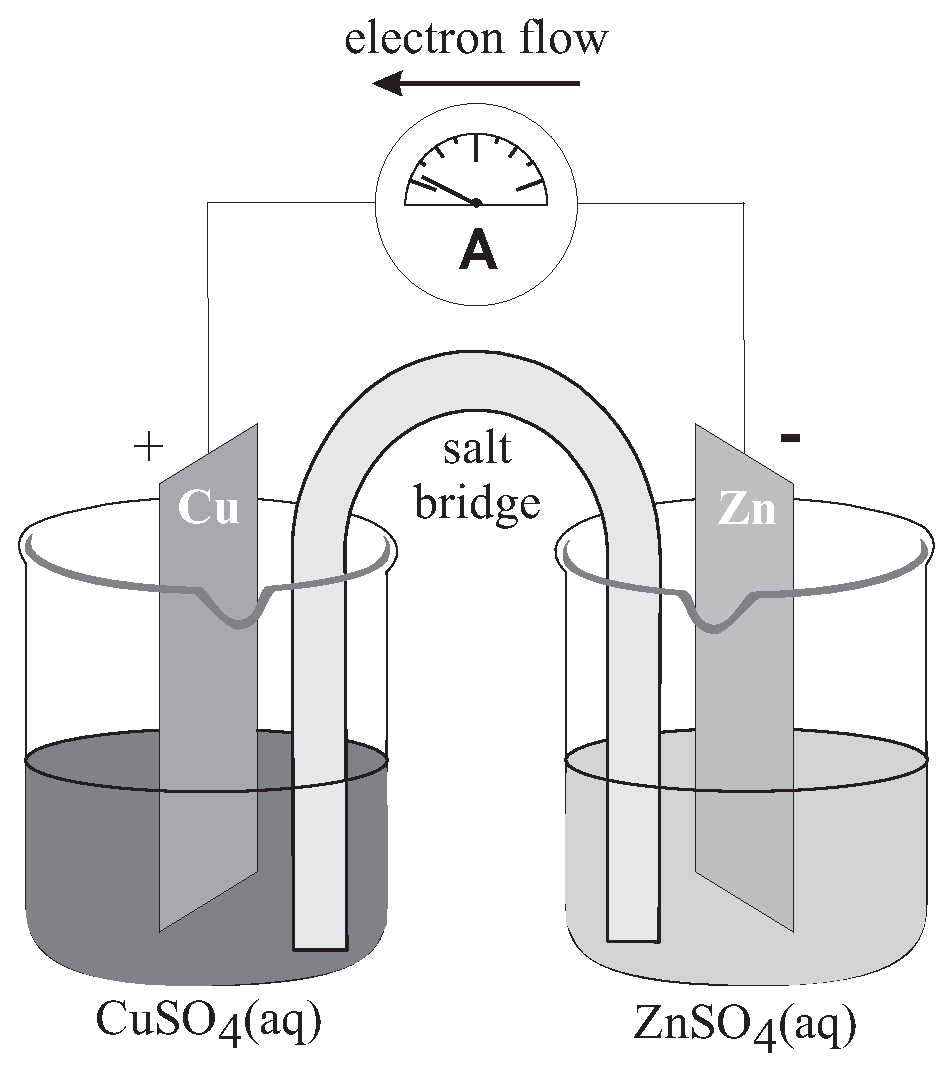
\includegraphics[width=6cm]{../../epsimages/VoltaicCellbw.eps}
\end{center}
}

\Results{

During the experiment, you should have noticed the following:

\begin{itemize}
\item{When the U-tube containing the Na$_{2}$SO$_{4}$ solution was absent, there was no reading on the ammeter.}
\item{When the U-tube was connected, a reading was recorded on the ammeter.}
\item{After the plates had been connected directly to each other and left for a day, there was a change in their mass. The mass of the zinc plate decreased, while the mass of the copper plate increased.}
\item{The direction of electron flow is from the zinc plate towards the copper plate.}
\end{itemize}
}

\Conclusions{

When a zinc sulphate solution containing a zinc plate is connected by a U-tube to a copper sulphate solution containing a copper plate, reactions occur in both solutions. The decrease in mass of the zinc plate suggests that the zinc metal has been oxidised. The increase in mass of the copper plate suggests that reduction has occurred here to produce more copper metal. This will be explained in detail below.}
}

\subsection{Half-cell reactions in the Zn-Cu cell}

The experiment above demonstrated a zinc-copper cell. This was made up of a zinc \textbf{half cell} and a copper \textbf{half cell}.

\Definition{Half cell}{
A half cell is a structure that consists of a conductive electrode surrounded by a conductive electrolyte. For example, a zinc half cell could consist of a zinc metal plate (the electrode) in a zinc sulphate solution (the electrolyte).
}

How do we explain what has just been observed in the zinc-copper cell?

\begin{itemize}
\item{\textit{Copper plate}

At the copper plate, there was an \textit{increase} in mass. This means that Cu$^{2+}$ ions from the copper sulphate solution were deposited onto the plate as atoms of copper metal. The half-reaction that takes place at the copper plate is:
\begin{center}
\rm${Cu^{2+} + 2e^{-} \rightarrow Cu}$ \textbf{(Reduction half reaction)}
\end{center}

Another shortened way to represent this copper half-cell is Cu$^{2+}$/Cu.
}

\item{\textit{Zinc plate}

At the zinc plate, there was a \textit{decrease} in mass. This means that some of the zinc goes into solution as Z$^{2+}$ ions. The electrons remain on the zinc plate, giving it a negative charge. The half-reaction that takes place at the zinc plate is:
\begin{center}
\rm${Zn \rightarrow Zn^{2+} + 2e^{-}}$ \textbf{(Oxidation half reaction)}
\end{center}

The shortened way to represent the zinc half-cell is Zn/Zn$^{2+}$.\\

The overall reaction is:

\begin{center}
\rm${Zn + Cu^{2+} + 2e^{-} \rightarrow Zn^{2+} + Cu + 2e^{-}}$ or, if we cancel the electrons:

\rm${Zn + Cu^{2+} \rightarrow Zn^{2+} + Cu}$ 
\end{center}

For this electrochemical cell, the standard notation is:
\begin{equation*}
Zn|Zn^{2+}||Cu^{2+}|Cu
\end{equation*}
where
\begin{eqnarray*}
  | &=& \rm{a \ phase \ boundary \ (solid/aqueous)}\\
  || & = & \rm{the \ salt \ bridge}
\end{eqnarray*}
}  
\end{itemize}

In the notation used above, the oxidation half-reaction at the anode is written on the left, and the reduction half-reaction at the cathode is written on the right. In the Zn-Cu electrochemical cell, the direction of current flow in the external circuit is from the zinc electrode (where there has been a build up of electrons) to the copper electrode.
 
\subsection{Components of the Zn-Cu cell}

In the zinc-copper cell, the copper and zinc plates are called the \textbf{electrodes}. The electrode where oxidation occurs is called the \textbf{anode}, and the electrode where reduction takes place is called the \textbf{cathode}. In the zinc-copper cell, the zinc plate is the anode and the copper plate is the cathode.

\Definition{Electrode}{An electrode is an electrical conductor that is used to make contact with a metallic part of a circuit. The anode is the electrode where oxidation takes place. The cathode is the electrode where reduction takes place. }

The zinc sulphate and copper sulphate solutions are called the \textbf{electrolyte} solutions.

\Definition{Electrolyte}{An electrolyte is a substance that contains free ions and which therefore behaves as an electrical conductor.}

The U-tube also plays a very important role in the cell. In the Zn/Zn$^{2+}$ half-cell, there is a build up of positive charge because of the release of electrons through oxidation. In the Cu$^{2+}$/Cu half-cell, there is a decrease in the positive charge because electrons are gained through reduction. This causes a movement of SO$_{4}^{2-}$ ions into the beaker where there are too many positive ions, in order to neutralise the solution. Without this, the flow of electrons in the outer circuit stops completely. The U-tube is called the \textbf{salt bridge}. The salt bridge acts as a transfer medium that allows ions to flow through without allowing the different solutions to mix and react. 

\Definition{Salt bridge}{A salt bridge, in electrochemistry, is a laboratory device that is used to connect the oxidation and reduction half-cells of a galvanic cell.}

\subsection{The Galvanic cell}

In the zinc-copper cell the important thing to notice is that the chemical reactions that take place at the two electrodes cause an electric current to flow through the outer circuit. In this type of cell, \textbf{chemical energy is converted to electrical energy}. These are called \textbf{galvanic cells}. The zinc-copper cell is one example of a galvanic cell. A galvanic cell (which is also sometimes referred to as a \textbf{voltaic} or \textbf{electrochemical} cell) consists of two metals that are connected by a salt bridge between the individual half-cells. A galvanic cell generates electricity using the reactions that take place at these two metals, each of which has a different \textbf{reaction potential}.\\

So what is meant by the 'reaction potential' of a substance? Every metal has a different half reaction and different dissolving rates. When two metals with different reaction potentials are used in a galvanic cell, a potential difference is set up between the two electrodes, and the result is a flow of current through the wire that connects the electrodes. In the zinc-copper cell, zinc has a higher reaction potential than copper and therefore dissolves more readily into solution. The metal 'dissolves' when it loses electrons to form positive metal ions. These electrons are then transferred through the connecting wire in the outer circuit. 

\Definition{Galvanic cell}{A galvanic (voltaic) cell is an electrochemical cell that uses a chemical reaction between two dissimilar electrodes dipped in an electrolyte, to generate an electric current.}

\begin{IFact}{It was the Italian physician and anatomist Luigi Galvani who marked the birth of electrochemistry by making a link between chemical reactions and electricity. In 1780, Galvani discovered that when two different metals (copper and zinc for example) were connected together and then both touched to different parts of a nerve of a frog leg at the same time, they made the leg contract. He called this "animal electricity". While many scientists accepted his ideas, another scientist, Alessandro Volta, did not. In 1800, because of his professional disagreement over the galvanic response that had been suggested by Luigi Galvani, Volta developed the \textit{voltaic pile}, which was very similar to the galvanic cell. It was the work of these two men that paved the way for all electrical batteries.}
\end{IFact}

\begin{wex}{Understanding galvanic cells\\}{
For the following cell:
\begin{center}
\begin{equation*}
Zn|Zn^{2+}||Ag^{+}|Ag
\end{equation*}
\end{center}
\begin{enumerate}
\item{Give the anode and cathode half-reactions.}
\item{Write the overall equation for the chemical reaction.}
\item{Give the direction of the current in the external circuit.}
\end{enumerate}
}

{\westep{Identify the oxidation and reduction reactions}

In the standard notation format, the oxidation reaction is written on the left and the reduction reaction on the right. So, in this cell, zinc is oxidised and silver ions are reduced.\\
\westep{Write the two half reactions}

Oxidation half-reaction:

\rm${Zn \rightarrow Zn^{2+} + 2e^{-}}$\\

Reduction half-reaction:

\rm${Ag^{+} + e^{-} \rightarrow Ag}$\\
\westep{Combine the half-reactions to get the overall equation.}

When you combine the two half-reactions, all the reactants must go on the left side of the equation and the products must go on the right side of the equation. The overall equation therefore becomes:

\begin{center}
$\rm{Zn + Ag^{+} + e^{-} \rightarrow Zn^{2+} + 2e^{-} + Ag}$
\end{center}

Note that this equation is not balanced. This will be discussed later in the chapter.\\
\westep{Determine the direction of current flow}

A build up of electrons occurs where oxidation takes place. This is at the zinc electrode. Current will therefore flow from the zinc electrode to the silver electrode.
}
\end{wex}

\subsection{Uses and applications of the galvanic cell}

The principles of the galvanic cell are used to make \textbf{electrical batteries}. In science and technology, a battery is a device that stores chemical energy and makes it available in an electrical form. Batteries are made of electrochemical devices such as one or more galvanic cells, fuel cells or flow cells. Batteries have many uses including in torches, electrical appliances (long-life alkaline batteries), digital cameras (lithium batteries), hearing aids (silver-oxide batteries), digital watches (mercury batteries) and military applications (thermal batteries). Refer to chapter \ref{chap:chemindustry} for more information on batteries.\\

The galvanic cell can also be used for \textbf{electroplating}. Electroplating occurs when an electrically conductive object is coated with a layer of metal using electrical current. Sometimes, electroplating is used to give a metal particular properties such as corrosion protection or wear resistance. At other times, it can be for aesthetic reasons for example in the production of jewellery. This will be discussed in more detail later in this chapter. 

\Exercise{Galvanic cells\\}{
\begin{enumerate}

\item{The following half-reactions take place in an electrochemical cell:

$\rm{Fe \rightarrow Fe^{3+} + 3e^{-}}$

$\rm{Fe^{2+} + 2e^{-} \rightarrow Fe}$\\

	\begin{enumerate}
	\item{Which is the oxidation half-reaction?}
	\item{Which is the reduction half-reaction?}
	\item{Name one oxidising agent.}
	\item{Name one reducing agent.}
	\item{Use standard notation to represent this electrochemical cell.}
	\end{enumerate}

}

\item{For the following cell:}

\begin{equation*}
Mg|Mg^{2+}||Mn^{2+}|Mn
\end{equation*}

	\begin{enumerate}
	
	\item{Give the cathode half-reaction.}
	\item{Give the anode half-reaction.}
	\item{Give the overall equation for the electrochemical cell.}
	\item{What metals could be used for the electrodes in this electrochemical cell?}
	\item{Suggest two electrolytes for this electrochemical cell.}
	\item{In which direction will the current flow?}
	\item{Draw a simple sketch of the complete cell.}
	\end{enumerate}

\item{For the following cell:}

\begin{equation*}
Sn|Sn^{2+}||Ag^{+}|Ag
\end{equation*}

\begin{enumerate}
	\item{Give the cathode half-reaction.}
	\item{Give the anode half-reaction.}
	\item{Give the overall equation for the electrochemical cell.}
	\item{Draw a simple sketch of the complete cell.}
	\end{enumerate}

\end{enumerate}

% Automatically inserted shortcodes - number to insert 3
\par \practiceinfo
\par \begin{tabular}[h]{cccccc}
% Question 1
(1.)	01qj	&
% Question 2
(2.)	01qk	&
% Question 3
(3.)	01qm	&
\end{tabular}
% Automatically inserted shortcodes - number inserted 3
}



% CHILD SECTION END 



% CHILD SECTION START 

\section{The Electrolytic cell}
\label{sec:electrochemical:electrolytic}

In section \ref{sec:electrochemical:galvanic}, we saw that a chemical reaction that involves a transfer of electrons, can be used to produce an electric current. In this section, we are going to see whether the 'reverse' process applies. In other words, is it possible to use an electric current to force a particular chemical reaction to occur, which would otherwise not take place? The answer is 'yes', and the type of cell that is used to do this, is called an \textbf{electrolytic cell}.

\Definition{Electrolytic cell}{An electrolytic cell is a type of cell that uses electricity to drive a non-spontaneous reaction.}

An electrolytic cell is activated by applying an electrical potential across the anode and cathode to force an internal chemical reaction between the ions that are in the electrolyte solution. This process is called \textbf{electrolysis}.

\Definition{Electrolysis}{In chemistry and manufacturing, electrolysis is a method of separating bonded elements and compounds by passing an electric current through them.}

\Activity{Demonstration}{The movement of coloured ions\\}{

A piece of filter paper is soaked in an ammonia-ammonium chloride solution and placed on a microscope slide. The filter paper is then connected to a supply of electric current using crocodile clips and connecting wire as shown in the diagram below. A line of copper chromate solution is placed in the centre of the filter paper. The colour of this solution is initially green-brown. \\

\begin{center}
\begin{pspicture}(-6,-2.3)(6,3.7)
%\psgrid
\psset{unit=0.8}
\rput(-7,0){
\pnode(0,0){A}
\pnode(5,0){B}
\pnode(5,0.5){C}
\pnode(0,0.5){D}
\pnode(1,3){E}
\pnode(6,3){F}
\pnode(6,2.5){G}
\psframe(A)(C)
\psline(D)(E)(F)(C)
\psline(B)(G)(F)
\psline(C)(D)
\psframe[fillstyle=solid,fillcolor=lightgray](2,0)(3,0.5)
\pspolygon[fillstyle=solid,fillcolor=lightgray](2,0.5)(3,3)(4,3)(3,0.5)
\psline[arrowsize=10pt,arrowinset=0,arrowlength=2.5]{->}(-0.5,-1)(-0.5,1.5)(1,1.5)
\psline[arrowsize=10pt,arrowinset=0,arrowlength=2.5]{<-}(5,1.5)(6.5,1.5)(6.5,-1)
\battery(-0.5,-1)(6.5,-1){}
\uput[u](3.5,3){copper chromate (green brown)}
\psline(3.5,3.2)(3.5,2.5)
\uput[d](3,-1.5){start of reaction}
\uput[u](0,1.5){\Large{\textbf{+}}}
\uput[u](6,1.5){\Large{\textbf{-}}}
\uput[ul](3,-0.8){\Large{\textbf{+}}}
\uput[ur](3,-0.8){\Large{\textbf{-}}}
}

\rput(1,0){
\pnode(0,0){A}
\pnode(5,0){B}
\pnode(5,0.5){C}
\pnode(0,0.5){D}
\pnode(1,3){E}
\pnode(6,3){F}
\pnode(6,2.5){G}
\psframe(A)(C)
\psline(D)(E)(F)(C)
\psline(B)(G)(F)
\psline(C)(D)
\psframe[fillstyle=solid,fillcolor=gray](3,0)(3.5,0.5)
\psframe[fillstyle=solid,fillcolor=lightgray](2,0)(3,0.5)
\psframe(1.5,0)(2,0.5)
\pspolygon[fillstyle=solid,fillcolor=lightgray](2,0.5)(3,3)(4,3)(3,0.5)
\pspolygon(1.5,0.5)(2.5,3)(3,3)(2,0.5)
\pspolygon[fillstyle=solid,fillcolor=gray](3,0.5)(3.5,0.5)(4.5,3)(4,3)

\psline[arrowsize=10pt,arrowinset=0,arrowlength=2.5]{->}(-0.5,-1)(-0.5,1.5)(1,1.5)
\psline[arrowsize=10pt,arrowinset=0,arrowlength=2.5]{<-}(5,1.5)(6.5,1.5)(6.5,-1)
\battery(-0.5,-1)(6.5,-1){}
\pcline{<-}(1,3.2)(2.5,3.2)
\aput{:U}{negative ions}
\pcline{->}(4.5,3.2)(6,3.2)
\aput{:U}{positive ions}
\uput[d](3,-1.5){after 20 minutes}
\uput[u](0,1.5){\Large{\textbf{+}}}
\uput[u](6,1.5){\Large{\textbf{-}}}
\uput[ul](3,-0.8){\Large{\textbf{+}}}
\uput[ur](3,-0.8){\Large{\textbf{-}}}
}
\end{pspicture}
\end{center}


The current is then switched on and allowed to run for about 20 minutes. After this time, the central coloured band disappears and is replaced by two bands, one yellow and the other blue, which seem to have separated out from the first band of copper chromate. \\

\textbf{Explanation:} 

\begin{itemize}
\item{The cell that is used to supply an electric current sets up a potential difference across the circuit, so that one of the electrodes is positive and the other is negative.}
\item{The chromate (CrO$_{4}^{2-}$) ions in the copper chromate solution are attracted to the positive electrode, while the Cu$^{2+}$ ions are attracted to the negative electrode.}
\end{itemize}

\textbf{Conclusion:\\}

The movement of ions occurs because the electric current in the outer circuit sets up a potential difference between the two electrodes.
}

Similar principles apply in the electrolytic cell, where substances that are made of ions can be broken down into simpler substances through electrolysis.

\subsection{The electrolysis of copper sulphate}

There are a number of examples of electrolysis. The electrolysis of copper sulphate is just one.

\Activity{Demonstration}{The electrolysis of copper sulphate\\}{

Two copper electrodes are placed in a solution of blue copper sulphate and are connected to a source of electrical current as shown in the diagram below. The current is turned on and the reaction is left for a period of time.\\

\begin{center}
\begin{pspicture}(-2,-0.2)(5,6.6)
%\psgrid
\rput(0,0){\psset{unit=2}\filledbeaker}
\psframe(0.25,1)(0.75,4.5)
\rput(2,0){\psframe(0.25,1)(0.75,4.5)}
\psline(0.5,4.5)(0.5,6)
\battery(0.5,6)(2.5,6){}
\psline(2.5,4.5)(2.5,6)
\uput[ul](0.5,4.5){\textbf{+}}
\uput[ur](2.5,4.5){\textbf{--}}
\uput[ul](1.4,6){\textbf{+}}
\uput[ur](1.6,6){\textbf{--}}
\uput[l](0,3){positive anode}
\psline(-0.1,3)(0.5,3)

\uput[r](3,3){negative cathode}
\psline(3.1,3)(2.5,3)

\uput[l](0,2){copper electrode}
\psline(-0.1,2)(0.5,2.2)
\uput[r](3,2){copper electrode}
\psline(3.1,2)(2.5,2.2)

\uput[r](3,0){CuSO$_4$ solution}
\psline(3.1,0.1)(1.5,0.1)

\rput(0.5,0.5){SO$_4^{2-}$}
\rput(2.5,0.5){Cu$^{2+}$}
\psarc{->}(1,1){0.4}{-90}{90}
\psarc{<-}(2,1){0.4}{90}{-90}

\end{pspicture}
\end{center}

\textbf{Observations:}

\begin{itemize}
\item{The initial blue colour of the solution remains unchanged.}
\item{It appears that copper has been \textit{deposited} on one of the electrodes but \textit{dissolved} from the other.\\}
\end{itemize}

\textbf{Explanation:\\}

\begin{itemize}
\item{At the negative cathode, positively charged Cu$^{2+}$ ions are attracted to the negatively charged electrode. These ions gain electrons and are reduced to form copper metal, which is deposited on the electrode. The half-reaction that takes place is as follows:

\begin{center}
\rm${Cu^{2+}(aq) + 2e^{-} \rightarrow Cu(s)}$ \textbf{(reduction half reaction)}
\end{center}
}

\item{At the positive anode, copper metal is oxidised to form Cu$^{2+}$ ions. This is why it appears that some of the copper has dissolved from the electrode. The half-reaction that takes place is as follows:

\begin{center}
\rm${Cu(s) \rightarrow Cu^{2+}(aq) + 2e^{-}}$ \textbf{(oxidation half reaction)}
\end{center}
}

\item{The amount of copper that is \textit{deposited} at one electrode is approximately the same as the amount of copper that is \textit{dissolved} from the other. The number of Cu$^{2+}$ ions in the solution therefore remains almost the same and the blue colour of the solution is unchanged.}
\end{itemize}

\textbf{Conclusion:}\\

In this demonstration, an electric current was used to split CuSO$_{4}$ into its component ions, Cu$^{2+}$ and SO$_{4}^{2-}$. This process is called \textit{electrolysis}.

}

\subsection{The electrolysis of water}

Water can also undergo electrolysis to form hydrogen gas and oxygen gas according to the following reaction:

\begin{center}
\rm${2H_{2}O(l) \rightarrow 2H_{2}(g) + O_{2}(g)}$
\end{center}

This reaction is very important because hydrogen gas has the potential to be used as an energy source. The electrolytic cell for this reaction consists of two electrodes (normally platinum metal), submerged in an electrolyte and connected to a source of electric current.\\

The reduction half-reaction that takes place at the cathode is as follows:
\begin{center}
\rm${2H_{2}O(l) + 2e^{-} \rightarrow H_{2}(g) + 2OH^{-}(aq)}$
\end{center}

The oxidation half-reaction that takes place at the anode is as follows:
\begin{center}
\rm${2H_{2}O(l) \rightarrow O_{2}(g) + 4H^{+}(aq) + 4e^{-}}$
\end{center}

\subsection{A comparison of galvanic and electrolytic cells}

It should be much clearer now that there are a number of differences between a \textit{galvanic} and an \textit{electrolytic} cell. Some of these differences have been summarised in table \ref{tab:electrochemical:comparison}.

\begin{table}[h]
\begin{center}
\begin{tabular}{|p{4cm}|p{4cm}|p{4cm}|}\hline
\textbf{Item} & \textbf{Galvanic cell} & \textbf{Electrolytic cell}\\\hline
Metals used for electrode & Two metals with different reaction potentials are used as electrodes & The same metal can be used for both the cathode and the anode \\\hline
Charge of the anode & negative & positive \\\hline
Charge of the cathode & positive & negative \\\hline
The electrolyte solution/s & The electrolyte solutions are kept separate from one another, and are connected only by a salt bridge & The cathode and anode are in the same electrolyte \\\hline
Energy changes & Chemical potential energy from chemical reactions is converted to electrical energy & An external supply of electrical energy causes a chemical reaction to occur \\\hline
Applications & Run batteries, electroplating & Electrolysis e.g. of water, NaCl \\\hline

\end{tabular}
\end{center}
\caption{A comparison of galvanic and electrolytic cells}
\label{tab:electrochemical:comparison}
\end{table} 

\Exercise{Electrolyis\\}{

\begin{enumerate}
\item{An electrolytic cell consists of two electrodes in a silver chloride (AgCl) solution, connected to a source of current. A current is passed through the solution and Ag$^{+}$ ions are reduced to a silver metal deposit on one of the electrodes.}
	\begin{enumerate}
	\item{Give the equation for the reduction half-reaction.}
	\item{Give the equation for the oxidation half-reacion.}
	\end{enumerate}

\item{Electrolysis takes place in a solution of molten lead bromide (PbBr) to produce lead atoms.}
	\begin{enumerate}
	\item{Draw a simple diagram of the electrolytic cell.}
	\item{Give equations for the half-reactions that take place at the anode and cathode, and include these in the diagram.}
	\item{On your diagram, show the direction in which current flows.}
	\end{enumerate}
\end{enumerate}

% Automatically inserted shortcodes - number to insert 2
\par \practiceinfo
\par \begin{tabular}[h]{cccccc}
% Question 1
(1.)	01qn	&
% Question 2
(2.)	01qp	&
\end{tabular}
% Automatically inserted shortcodes - number inserted 2
}



% CHILD SECTION END 



% CHILD SECTION START 

\section{Standard Electrode Potentials}
\label{sec:electrochemical:potentials}



If a voltmeter is connected in the circuit of an electrochemical cell, a reading is obtained. In other words, there is a \textbf{potential difference} between the two half cells. In this section, we are going to look at this in more detail to try to understand more about the \textbf{electrode potentials} of each of the electrodes in the cell. We are going to break this section down so that you build up your understanding gradually. Make sure that you understand each subsection fully before moving on, otherwise it might get confusing!

\subsection{The different reactivities of metals}
\label{subsec:electrochemical:metal reactivity}

All metals have different reactivities. When metals react, they give away electrons and form positive ions. But some metals do this more easily than others. Look at the following two half reactions:

\begin{center}
\rm${Zn \rightarrow Zn^{2+} + 2e^{-}}$

\rm${Cu \rightarrow Cu^{2+} + 2e^{-}}$
\end{center}

Of these two metals, zinc is more reactive and is more likely to give away electrons to form Zn$^{2+}$ ions in solution, than is copper.

\subsection{Equilibrium reactions in half cells}
\label{subsec:electrochemical:equilibrium reactions}

Let's think back to the Zn-Cu electrochemical cell. This cell is made up of two half cells and the reactions that take place at each of the electrodes are as follows:

\begin{center}
\rm${Zn \rightarrow Zn^{2+} + 2e^{-}}$

\rm${Cu^{2+} + 2e^{-} \rightarrow Cu}$
\end{center}

At the zinc electrode, the zinc metal loses electrons and forms Zn$^{2+}$ ions. The electrons are concentrated on the zinc metal while the Zn$^{2+}$ ions are in solution. But some of the ions will be attracted back to the negatively charged metal, will gain their electrons again and will form zinc metal. A \textbf{dynamic equilibrium} is set up between the zinc metal and the Zn$^{2+}$ ions in solution when the rate at which ions are \textit{leaving} the metal is equal to the rate at which they are \textit{joining} it again. The situation looks something like the diagram in figure \ref{fig:electrochemical:zinc}.

\begin{figure}[h]
\begin{center}
\begin{pspicture}(-2,1)(6,6)
%\psgrid[gridcolor=lightgray]
\psline(0,1)(0,4)
\psline(4,1)(4,4)
\psline(0,1)(4,1)
\psframe(1.5,2)(2.5,5)
\psline(0,3)(1.5,3)
\psline(2.5,3)(4,3)
\rput(1.8,3.5){\Large\textbf{-}}
\rput(1.9,4){\Large\textbf{-}}
\rput(2.1,3.7){\Large\textbf{-}}
\rput(1.7,3.2){\Large\textbf{-}}
\rput(2.3,4.4){\Large\textbf{-}}
\rput(2.3,4.3){\Large\textbf{-}}
\rput(1.9,2.2){\Large\textbf{-}}
\rput(1.7,3.2){\Large\textbf{-}}
\rput(2,3.4){\Large\textbf{-}}
\rput(2.4,2.4){\Large\textbf{-}}
\rput(2.3,2.3){\Large\textbf{-}}
\rput(2,2.5){\Large\textbf{-}}

\rput(2.9,2.3){\textbf{2+}}
\rput(2.8,1.5){\textbf{2+}}
\rput(2.3,1.8){\textbf{2+}}
\rput(1.6,1.5){\textbf{2+}}
\rput(1.3,2.6){\textbf{2+}}
\psline(3.2,2.3)(4.2,2.3)
\rput(6.2,2.3){Zn$^{2+}$ ions in solution}
\psline(2,4.5)(4.2,4.5)
\rput(5.3,4.5){zinc metal}
\psline(2,3.5)(4.2,3.5)
\rput(8,3.5){concentration of electrons on metal surface}
\end{pspicture}
\caption{Zinc loses electrons to form positive ions in solution. The electrons accumulate on the metal surface.}
\label{fig:electrochemical:zinc}
\end{center}
\end{figure}

The equilibrium reaction is represented like this:

\begin{center}
\rm${Zn^{2+}(aq) + 2e^{-} \rightleftharpoons Zn(s)}$
\end{center}

(NOTE: By convention, the ions are written on the \textit{left} hand side of the equation)\\

In the zinc half cell, the equilibrium lies far to the left because the zinc loses electrons easily to form Zn$^{2+}$ ions. We can also say that the zinc is \textit{oxidised} and that it is a strong \textit{reducing agent}.\\

At the copper electrode, a similar process takes place. The difference though is that copper is not as reactive as zinc and so it does not form ions as easily. This means that the build up of electrons on the copper electrode is less (figure \ref{fig:electrochemical:copper}). \\ 

\begin{figure}[h]
\begin{center}
\begin{pspicture}(-2,1)(6,6)
%\psgrid[gridcolor=lightgray]
\psline(0,1)(0,4)
\psline(4,1)(4,4)
\psline(0,1)(4,1)
\psframe(1.5,2)(2.5,5)
\psline(0,3)(1.5,3)
\psline(2.5,3)(4,3)
\rput(1.9,4){\Large\textbf{-}}
\rput(2.1,3.7){\Large\textbf{-}}
\rput(1.7,3.2){\Large\textbf{-}}
\rput(2.3,4.3){\Large\textbf{-}}
\rput(1.7,3.2){\Large\textbf{-}}
\rput(2.3,2.3){\Large\textbf{-}}
\rput(2,2.5){\Large\textbf{-}}

\rput(2.3,1.8){\textbf{2+}}
\rput(1.6,1.5){\textbf{2+}}
\psline(2.7,1.8)(4.2,1.8)
\rput(6.2,2.3){Cu$^{2+}$ ions in solution}
\psline(2,4.5)(4.2,4.5)
\rput(5.3,4.5){copper metal}
\psline(2,3.5)(4.2,3.5)
\rput(8,3.5){concentration of electrons on metal surface}
\end{pspicture}
\caption{Zinc loses electrons to form positive ions in solution. The electrons accumulate on the metal surface.}
\label{fig:electrochemical:copper}
\end{center}
\end{figure}

The equilibrium reaction is shown like this:

\begin{center}
\rm${Cu^{2+}(aq) + 2e^{-} \rightleftharpoons Cu(s)}$
\end{center}

The equation lies far to the right because most of the copper is present as copper metal rather than as Cu$^{2+}$ ions. In this half reaction, the Cu$^{2+}$ ions are \textit{reduced}.

\subsection{Measuring electrode potential}
\label{subsec:electrochemical:measuring electrode potential}

If we put the two half cells together, a potential difference is set up in two places in the Zn-Cu cell:
\begin{enumerate}
\item{There is a potential difference between the metal and the solution surrounding it because one is more negative than the other.}
\item{There is a potential difference between the Zn and Cu electrodes because one is more negative than the other.}
\end{enumerate}

It is the \textbf{potential difference} (recorded as a voltage) between the two electrodes that causes electrons, and therefore current, to flow from the more negative electrode to the less negative electrode.\\

The problem though is that we cannot measure the potential difference (voltage) between a metal and its surrounding solution in the cell. To do this, we would need to connect a voltmeter to both the metal and the solution, which is not possible. This means we cannot measure the exact \textbf{electrode potential} (E$^{o}$V) of a particular metal. The electrode potential describes the ability of a metal to give up electrons. And if the exact electrode potential of each of the electrodes involved can't be measured, then it is difficult to calculate the potential difference between them. But what we \textit{can} do is to try to describe the electrode potential of a metal \textit{relative} to another substance. We need to use a \textbf{standard reference electrode} for this.

\subsection{The standard hydrogen electrode}
\label{subsec:electrochemical:hydrogen electrode}

Before we look at the standard hydrogen electrode, it may be useful to have some more understanding of the ideas behind a 'reference electrode'. Refer to the Tip box on 'Understanding the ideas behind a reference electrode' before you read further.

\Tip{Understanding the ideas behind a reference electrode}{\textit{Adapted from www.chemguide.co.uk}\\

Let's say that you have a device that you can use to measure heights from some distance away. You want to use this to find out how tall a particular person is. Unfortunately, you can't see their feet because they are standing in long grass. Although you can't measure their absolute height, what you can do is to measure their height relative to the post next to them. Let's say that person A for example is 15 cm \textit{shorter} than the height of the post. You could repeat this for a number of other people (B and C). Person B is 30 cm shorter than the post and person C is 10 cm \textit{taller} than the post.

\begin{center}
\begin{pspicture}(-3,-5)(6,3)
%\psgrid[gridcolor=lightgray]
\def\stickman{
\pscircle(2,2){0.4}
\psline(2,1.6)(2,0.6)
\psline(2,0.6)(1.3,0)
\psline(2,0.6)(2.7,0)
\psline(1.5,1.2)(2.5,1.2)
}
\rput(0,0){\stickman}
\psline(0,0)(3.2,0)
\psframe[fillstyle=solid,fillcolor=darkgray](3.2,0)(3.5,2.7)
\rput(0,-0.3){\textbf{A}}
\rput(-2,-4){
\rput(0,0){\psset{unit=0.8}\stickman}
\psline(0,0)(3.2,0)
\psframe[fillstyle=solid,fillcolor=darkgray](3.2,0)(3.5,2.7)
\rput(0,-0.3){\textbf{B}}
}
\rput(2,-4){
\rput(0,0){\psset{unit=1.2}\stickman}
\psline(0,0)(3.2,0)
\psframe[fillstyle=solid,fillcolor=darkgray](3.2,0)(3.5,2.7)
\rput(0,-0.3){\textbf{C}}
}
\end{pspicture}
\end{center}

You could summarise your findings as follows:

\begin{center}
\begin{tabular}{|c|c|}\hline
\textbf{Person} & \textbf{Height relative to post (cm)}\\\hline
A & -15 \\\hline
B & -30 \\\hline
C & +10 \\\hline
\end{tabular}
\end{center}



Although you don't know any of their absolute heights, you can rank them in order, and do some very simple sums to work out exactly how much taller one is than another. For example, person C is 25 cm taller than A and 40 cm taller than B.
}

As mentioned earlier, it is difficult to measure the \textit{absolute} electrode potential of a particular substance, but we can use a reference electrode (similar to the 'post' in the Tip box example) that we use to calculate \textit{relative} electrode potentials for these substances. The reference elctrode that is used is the \textbf{standard hydrogen electrode} (figure \ref{fig:electrochemical:hydrogen electrode}).

\Definition{Standard hydrogen electrode\\}{
The standard hydrogen electrode is a redox electrode which forms the basis of the scale of oxidation-reduction potentials. The actual electrode potential of the hydrogen electrode is estimated to be 4.44 � $\pm$ 0.02 V at 25$^{0}$C, but its standard electrode potential is said to be zero at all temperatures so that it can be used as for comparison with other electrodes. The hydrogen electrode is based on the following redox half cell:

\begin{center}
   $\rm{2H^{+}(aq) + 2e^{-} \rightarrow H_{2}(g)}$
\end{center}
} % end of the definition

\begin{figure}[h]
\begin{center}
\scalebox{1.3} % Change this value to rescale the drawing.
{
\begin{pspicture}(0,-3.5848436)(10.2864065,3.5648437)
\psline[linewidth=0.04cm](4.4370313,1.6848439)(4.4379997,-2.5351562)
\psline[linewidth=0.04cm](7.657031,-2.5151563)(7.657031,1.6848439)
\psline[linewidth=0.04cm](4.597031,1.2048438)(7.48,1.2048438)
\psline[linewidth=0.04cm](7.48,1.2048438)(7.657031,1.3648437)
\psline[linewidth=0.04cm](4.597031,1.2048439)(4.44,1.3648437)
\psline[linewidth=0.04cm](5.74,-1.1151563)(6.4570312,-1.1151563)
\psline[linewidth=0.04cm](6.4570312,-1.1151563)(6.4370313,-0.0351562)
\psline[linewidth=0.04cm](5.977031,-0.31515622)(5.977031,-0.7551562)
\psline[linewidth=0.04cm](5.977031,-0.7551562)(6.217031,-0.7551562)
\psline[linewidth=0.04cm](6.217031,-0.7551562)(6.217031,-0.3351562)
\psline[linewidth=0.04cm](6.217031,-0.3351562)(5.977031,-0.3351562)
\psline[linewidth=0.04cm](6.077031,-0.3351562)(6.077031,3.5248437)
\psline[linewidth=0.04cm](6.4370313,-0.05515619)(6.257031,0.2448438)
\psline[linewidth=0.04cm](5.9370313,0.22484376)(5.9370313,3.0048437)
\psline[linewidth=0.04cm](6.2570314,0.22484376)(6.2370315,3.1648438)
\psline[linewidth=0.04cm](6.2370315,3.1448438)(5.7370315,3.5448437)
\psline[linewidth=0.04cm](5.9379997,3.0048437)(5.52,3.2848437)
\psline[linewidth=0.04cm](5.517031,3.2848437)(4.117031,3.2848437)
\psline[linewidth=0.04cm](5.7570314,3.5448437)(4.157031,3.5448437)
\psline[linewidth=0.04cm](4.32,2.8048437)(5.12,2.8048437)
\psline[linewidth=0.04cm](4.317031,2.5048437)(4.977031,2.5048437)
\psline[linewidth=0.04cm](4.96,2.5248437)(5.08,2.3248436)
\psline[linewidth=0.04cm](5.12,2.8048437)(5.317031,2.5048437)
\psline[linewidth=0.04cm](5.3170314,2.5048437)(5.32,-1.2551563)
\psline[linewidth=0.04cm](5.077031,2.324844)(5.08,-1.2751563)
\psline[linewidth=0.04cm](4.4379997,1.6848438)(4.22,1.9048438)
\psline[linewidth=0.04cm,arrowsize=0.05291667cm 2.0,arrowlength=1.4,arrowinset=0.4]{->}(3.8570313,2.6448438)(4.68,2.6448438)
\psline[linewidth=0.04cm,arrowsize=0.05291667cm 2.0,arrowlength=1.4,arrowinset=0.4]{<-cc}(3.96,3.4248438)(4.597031,3.4248438)
\psdots[dotsize=0.12](6.077031,3.3448436)
\psdots[dotsize=0.08,fillstyle=solid,dotstyle=o](5.9170313,-0.9551562)
\psdots[dotsize=0.08,fillstyle=solid,dotstyle=o](6.317031,-0.8151562)
\psdots[dotsize=0.08,fillstyle=solid,dotstyle=o](6.297031,-0.2751562)
\psdots[dotsize=0.08,fillstyle=solid,dotstyle=o](5.9570312,-0.0751562)
\psdots[dotsize=0.08,fillstyle=solid,dotstyle=o](6.057031,-0.9551562)
\usefont{T1}{ptm}{m}{n}
\rput(8.621407,0.4698438){\small [H$_3$O$^+$]}
\usefont{T1}{ptm}{m}{n}
\rput(8.676406,0.0098438){\small (1 mol.dm$^{-3}$)}
\usefont{T1}{ptm}{m}{n}
\rput(8.644531,-0.4501562){\small 25 $^{\circ}$C}
\psline[linewidth=0.04cm](4.4570312,-2.5151563)(7.657031,-2.5151563)
\usefont{T1}{ptm}{m}{n}
\rput(3.5492187,-0.5301562){\small Pt}
\usefont{T1}{ptm}{m}{n}
\rput(2.722656,2.6698437){\small H$_2$ gas}
\usefont{T1}{ptm}{m}{n}
\rput(2.2823439,2.1898437){\small (1 x atmosphereric pressure)}
\psline[linewidth=0.04cm](3.8170311,-0.49515623)(6.097031,-0.5351562)
\usefont{T1}{ptm}{m}{n}
\psline[linewidth=0.04cm](5.7370315,-1.1151563)(5.7170315,-0.04515625)
\psline[linewidth=0.04cm](5.722467,-0.045392893)(5.9315953,0.23508051)
\psarc[linewidth=0.04](5.63,-1.2451563){0.31}{180.0}{356.9872}
\psarc[linewidth=0.04](5.62,-1.2351563){0.54}{180.0}{356.9872}
\psline[linewidth=0.04cm](5.92,-1.2751563)(6.18,-1.2751563)
\psline[linewidth=0.04cm](7.658,1.6848438)(7.858,1.9048438)
\psline[linewidth=0.04cm](7.92,0.5048438)(6.82,0.5048438)
\end{pspicture} 
}
\end{center}
\caption{The standard hydrogen electrode}
\label{fig:electrochemical:hydrogen electrode}
\end{figure}

A standard hydrogen electrode consists of a platinum electrode in a solution containing H$^{+}$ ions. The solution (e.g. H$_{2}$SO$_{4}$) that contains the H$^{+}$ ions has a concentration of 1 mol.dm$^{-3}$. As the hydrogen gas bubbles over the platinum electrode, an equilibrium is set up between hydrogen molecules and hydrogen ions in solution. The reaction is as follows:

\begin{center}
\rm${2H^{+}(aq) + 2e^{-} \rightleftharpoons H_{2}(g)}$
\end{center}

The position of this equilibrium can change if you change some of the conditions (e.g. concentration, temperature). It is therefore important that the conditions for the standard hydrogen electrode are standardised as follows: pressure = 100 kPa (1atm); temperature = 298 K (25$^{0}$C) and concentration = 1 mol.dm$^{-3}$.

In order to \textit{use} the hydrogen electrode, it needs to be attached to the electrode system that you are investigating. For example, if you are trying to determine the electrode potential of copper, you will need to connect the copper half cell to the hydrogen electrode; if you are trying to determine the electrode potential of zinc, you will need to connect the zinc half cell to the hydrogen electrode and so on. Let's look at the examples of zinc and copper in more detail.

\begin{enumerate}
\item{\textbf{Zinc}

Zinc has a greater tendency than hydrogen to form ions, so if the standard hydrogen electrode is connected to the zinc half cell, the zinc will be relatively more negative because the electrons that are released when zinc is oxidised will accumulate on the metal. The equilibria on the two electrodes are as follows:

\begin{center}
\rm${Zn^{2+}(aq) + 2e^{-} \rightleftharpoons Zn(s)}$

\rm${2H^{+}(aq) + 2e^{-} \rightleftharpoons H_{2}(g)}$
\end{center}

In the zinc half-reaction, the equilibrium lies far to the left and in the hydrogen half-reaction, the equilibrium lies far to the right. A simplified representation of the cell is shown in figure \ref{fig:zinc hydrogen}. 

\begin{figure}[h]
\begin{center}
\begin{pspicture}(-2,0)(6,5)
%\psgrid[gridcolor=lightgray]
\psframe(0,0)(1,2)
\psframe(3,0)(4,2)
\psline(0.5,2)(0.5,4)

\psline(3.5,2)(3.5,4)
\psline(0.5,4)(1.5,4)
\psline(3.5,4)(2.5,4)
\pscircle(2,4){0.5}
\rput(2,4){\textbf{V}}
\rput(0.7,1.7){\Large\textbf{-}}
\rput(0.2,1.2){\Large\textbf{-}}
\rput(0.5, 0.5){\Large\textbf{-}}
\rput(3.7,1.7){\Large\textbf{-}}
\rput(3.2,1.2){\Large\textbf{-}}
\rput(3.5, 0.5){\Large\textbf{-}}
\rput(3.7,0.7){\Large\textbf{-}}
\rput(3.6,0.3){\Large\textbf{-}}
\rput(3.6,1.6){\Large\textbf{-}}
\rput(3.5,1){\Large\textbf{-}}
\rput(-1,1.5){H electrode}
\rput(-1,1.2){(less negative)}
\rput(6.5,1.5){Zn electrode with electrons}

\end{pspicture}
\end{center}
\caption{When zinc is connected to the standard hydrogen electrode, relatively few electrons build up on the platinum (hydrogen) electrode. There are lots of electrons on the zinc electrode.}
\label{fig:zinc hydrogen}
\end{figure}


The voltmeter measures the potential difference between the charge on these electrodes. In this case, the voltmeter would read 0.76 and would show that Zn is the negative electrode (i.e. it has a relatively higher number of electrons).
}

\item{\textbf{Copper}

Copper has a lower tendency than hydrogen to form ions, so if the standard hydrogen electrode is connected to the copper half cell, the hydrogen will be relatively more negative. The equilibria on the two electrodes are as follows:

\begin{center}
\rm${Cu^{2+}(aq) + 2e^{-} \rightleftharpoons Cu(s)}$

\rm${2H^{+}(aq) + 2e^{-} \rightleftharpoons H_{2}(g)}$
\end{center}

In the copper half-reaction, the equilibrium lies far to the right and in the hydrogen half-reaction, the equilibrium lies far to the left. A simplified representation of the cell is shown in figure \ref{fig:copper hydrogen}. 

\begin{figure}[h]
\begin{center}
\begin{pspicture}(-2,0)(6,5)
%\psgrid[gridcolor=lightgray]
\psframe(0,0)(1,2)
\psframe(3,0)(4,2)
\psline(0.5,2)(0.5,4)
\psline(3.5,2)(3.5,4)
\psline(0.5,4)(1.5,4)
\psline(3.5,4)(2.5,4)
\pscircle(2,4){0.5}
\rput(2,4){\textbf{V}}
\rput(0.7,1.7){\Large\textbf{-}}
\rput(0.2,1.2){\Large\textbf{-}}
\rput(0.5, 0.5){\Large\textbf{-}}
\rput(3.7,1.7){\Large\textbf{-}}
\rput(3.2,1.2){\Large\textbf{-}}
\rput(3.5, 0.5){\Large\textbf{-}}
\rput(0.7,0.7){\Large\textbf{-}}
\rput(0.6,0.3){\Large\textbf{-}}
\rput(0.6,1.6){\Large\textbf{-}}
\rput(0.5,1){\Large\textbf{-}}
\rput(-1,1.5){H electrode}
\rput(5,1.5){Cu electrode}
\end{pspicture}
\end{center}
\caption{When copper is connected to the standard hydrogen electrode, relatively few electrons build up on the copper electrode. There are lots of electrons on the hydrogen electrode.}
\label{fig:copper hydrogen}
\end{figure}


The voltmeter measures the potential difference between the charge on these electrodes. In this case, the voltmeter would read 0.34 and would show that Cu is the positive electrode (i.e. it has a relatively lower number of electrons).
} 
\end{enumerate}

% All good up to here - MH 26/04 - except for incorrect Tip usage but won't stop compile

\subsection{Standard electrode potentials}
\label{subsec:electrochemical:standard potentials}

The voltages recorded earlier when zinc and copper were connected to a standard hydrogen electrode are in fact the \textbf{standard electrode potentials} for these two metals. It is important to remember that these are not \textit{absolute} values, but are potentials that have been measured \textit{relative} to the potential of hydrogen if the standard hydrogen electrode is taken to be zero. 

\Tip{Conventions and voltage sign\\}{By convention, the hydrogen electrode is written on the \textit{left hand side} of the cell. The sign of the voltage tells you the sign of the metal electrode.\\

In the examples we used earlier, zinc's electrode potential is actually -0.76 and copper is +0.34. So, if a metal has a \textit{negative} standard electrode potential, it means it forms ions easily. The more negative the value, the easier it is for that metal to form ions. If a metal has a \textit{positive} standard electrode potential, it means it does not form ions easily. This will be explained in more detail below.} 

Luckily for us, we do not have to calculate the standard electrode potential for every metal. This has been done already and the results are recorded in a table of standard electrode potentials (table \ref{tab:electrochemical:table sep}).\\

\begin{table}
\begin{center}
\begin{tabular}{|l|l|}\hline 
\textbf{Half-Reaction}
&
\textbf{$E^{0}V$} \\ \hline\hline
$Li^{+} + e^{-} \rightleftharpoons Li$ & -3.04 \\ \hline
$K^{+} + e^{-} \rightleftharpoons K $& -2.92 \\ \hline
$Ba^{2+} + 2e^{-} \rightleftharpoons Ba $& -2.90 \\ \hline
$Ca^{2+} + 2e^{-} \rightleftharpoons Ca $& -2.87 \\ \hline
$Na^{+} + e^{-} \rightleftharpoons Na $& -2.71 \\ \hline
$Mg^{2+} + 2e^{-} \rightleftharpoons Mg $& -2.37 \\ \hline
$Mn^{2+} + 2e^{-} \rightleftharpoons Mn $& -1.18 \\ \hline
$2H2O + 2e^{-} \rightleftharpoons H_{2} (g) + 2 OH^{-} $& -0.83 \\ \hline
$Zn^{2+} + 2e^{-} \rightleftharpoons Zn $& -0.76 \\ \hline
$Cr^{2+} + 2e^{-} \rightleftharpoons Cr $& -0.74 \\ \hline
$Fe^{2+} + 2e^{-} \rightleftharpoons Fe $& -0.44 \\ \hline
$Cr^{3+} + 3e^{-} \rightleftharpoons Cr $& -0.41 \\ \hline
$Cd^{2+} + 2e^{-} \rightleftharpoons Cd $& -0.40\\ \hline
$Co^{2+} + 2e^{-} \rightleftharpoons Co $& -0.28 \\ \hline
$Ni^{2+} + 2e^{-} \rightleftharpoons Ni $& -0.25 \\ \hline
$Sn^{2+} + 2e^{-} \rightleftharpoons Sn $& -0.14 \\ \hline
$Pb^{2+} + 2e^{-} \rightleftharpoons Pb $& -0.13 \\ \hline
$Fe^{3+} + 3e^{-} \rightleftharpoons Fe $& -0.04 \\ \hline
$2H^{+} + 2e^{-} \rightleftharpoons H_{2} (g) $& \textbf{0.00} \\ \hline
$S + 2H^{+} + 2e^{-} \rightleftharpoons H_{2}S (g) $& 0.14 \\ \hline
$Sn^{4+} + 2e^{-} \rightleftharpoons Sn^{2+} $& 0.15 \\ \hline
$Cu^{2+} + e^{-} \rightleftharpoons Cu^{+} $& 0.16 \\ \hline
$SO_{4}^{2+} + 4H^{+} + 2e^{-} \rightleftharpoons SO_{2} (g) + 2H_{2}O $& 0.17 \\ \hline
$Cu^{2+} + 2e^{-} \rightleftharpoons Cu $& 0.34 \\ \hline
$2H_{2}O + O_{2} + 4e^{-} \rightleftharpoons 4OH^{-} $& 0.40 \\ \hline
$Cu^{+} + e^{-} \rightleftharpoons Cu $& 0.52 \\ \hline
$I_{2} + 2e^{-} \rightleftharpoons 2I^{-} $& 0.54 \\ \hline
$O_{2} (g) + 2H^{+} + 2e^{-} \rightleftharpoons H_{2}O_{2} $& 0.68 \\ \hline
$Fe^{3+} + e^{-} \rightleftharpoons Fe^{2+}  $& 0.77 \\ \hline
$NO_{3}^{-} + 2H^{+} + e^{-} \rightleftharpoons NO_{2} (g) + H_{2}O $& 0.78 \\ \hline
$Hg^{2+} + 2e^{-} \rightleftharpoons Hg (l) $& 0.78 \\ \hline
$Ag^{+} + e^{-} \rightleftharpoons Ag $& 0.80 \\ \hline
$NO_{3}^{-} + 4H^{+} +3 e^{-} \rightleftharpoons NO (g) + 2H_{2}O $& 0.96 \\ \hline
$Br_{2} + 2e^{-} \rightleftharpoons 2Br^{-} $& 1.06 \\ \hline
$O_{2} (g) + 4H^{+} + 4e^{-} \rightleftharpoons 2H_{2}O $& 1.23 \\ \hline
$MnO_{2} + 4H^{+} + 2e^{-} \rightleftharpoons Mn^{2+} + 2H_{2}O $& 1.28 \\ \hline
$Cr_{2}O_{7}^{2-} + 14H^{+} + 6e^{-} \rightleftharpoons 2Cr^{3+} + 7H_{2}O $& 1.33 \\ \hline
$Cl_{2} + 2e^{-} \rightleftharpoons 2Cl^{-} $& 1.36 \\ \hline
$Au^{3+} + 3e^{-} \rightleftharpoons Au $& 1.50 \\ \hline
$MnO_{4}^{-} + 8H^{+} + 5e^{-} \rightleftharpoons Mn^{2+} + 4H_{2}O $& 1.52 \\ \hline
$Co^{3+} + e^{-} \rightleftharpoons Co^{2+} $& 1.82 \\ \hline
$F_{2} + 2e^{-} \rightleftharpoons 2F^{-} $& 2.87 \\ \hline
\end{tabular}
\end{center}
\caption{Standard Electrode Potentials} 
\label{tab:electrochemical:table sep}
\end{table}

A few examples from the table are shown in table \ref{tab:electrochemical:table sep abbrev}. These will be used to explain some of the trends in the table of electrode potentials.

\begin{table}[h]
\begin{center}
\begin{tabular}{|l|l|}\hline 
\textbf{Half-Reaction}
&
\textbf{$E^{0}V$} \\ \hline\hline
$Li^{+} + e^{-} \rightleftharpoons Li$ & -3.04 \\ \hline
$Zn^{2+} + 2e^{-} \rightleftharpoons Zn $& -0.76 \\ \hline
$Fe^{3+} + 3e^{-} \rightleftharpoons Fe $& -0.04 \\ \hline
$2H^{+} + 2e^{-} \rightleftharpoons H_{2} (g) $& \textbf{0.00} \\ \hline
$Cu^{2+} + 2e^{-} \rightleftharpoons Cu $& 0.34 \\ \hline
$Hg^{2+} + 2e^{-} \rightleftharpoons Hg (l) $& 0.78 \\ \hline
$Ag^{+} + e^{-} \rightleftharpoons Ag $& 0.80 \\ \hline
\end{tabular}
\end{center}
\caption{A few examples from the table of standard electrode potentials}
\label{tab:electrochemical:table sep abbrev}
\end{table}

Refer to table \ref{tab:electrochemical:table sep abbrev} and notice the following trends:

\begin{itemize}
\item{Metals at the top of series (e.g. Li) have more negative values. This means they ionise easily, in other words, they release electrons easily. These metals are easily \textbf{oxidised} and are therefore good \textbf{reducing agents}.}
\item{Metal ions at the bottom of the table are good at picking up electrons. They are easily \textbf{reduced} and are therefore good \textbf{oxidising agents}.}
\item{The reducing ability (i.e. the ability to act as a reducing agent) of the metals in the table \textit{increases} as you move \textit{up} in the table.}
\item{The oxidising ability of metals \textit{increases} as you move \textit{down} in the table.}
\end{itemize}

\begin{wex}{Using the table of Standard Electrode Potentials\\}{

The following half-reactions take place in an electrochemical cell:

$\rm{Cu^{2+} + 2e^{-} \rightleftharpoons Cu}$

$\rm{Ag^{-} + e^{-} \rightleftharpoons Ag}$\\

	\begin{enumerate}
	\item{Which of these reactions will be the oxidation half-reaction in the cell?}
	\item{Which of these reactions will be the reduction half-reaction in the cell?}
	\end{enumerate}
}
{
\westep{Determine the electrode potential for each metal}

From the table of standard electrode potentials, the electrode potential for the copper half-reaction is +0.34 V. The electrode potential for the silver half-reaction is +0.80 V.\\

\westep{Use the electrode potential values to determine which metal is oxidised and which is reduced}

Both values are positive, but silver has a higher positive electrode potential than copper. This means that silver does not form ions easily, in other words, silver is more likely to be \textit{reduced}. Copper is more likely to be \textit{oxidised} and to form ions more easily than silver. Copper is the oxidation half-reaction and silver is the reduction half-reaction.
}
\end{wex}

\Tip{Learning to understand the question in a problem.\\ Before you tackle this problem, make sure you understand exactly what the question is asking. If magnesium is able to displace silver from a solution of silver nitrate, this means that magnesium metal will form magnesium ions and the silver ions will become silver metal. In other words, there will now be \textit{silver} metal and a solution of \textit{magnesium nitrate}. This will only happen if magnesium has a greater tendency than silver to form ions. In other words, what the question is actually asking is whether magnesium or silver forms ions more easily.
}

\begin{wex}{Using the table of Standard Electrode Potentials\\}{
Is magnesium able to displace silver from a solution of silver nitrate?}
{ % start answer

\westep{Determine the half-reactions that would take place if magnesium were to displace silver nitrate.}

The half-reactions are as follows:

\rm${Mg^{2+} + 2e^{-} \rightleftharpoons Mg}$

\rm${Ag^{+} + e^{-} \rightleftharpoons Ag}$\\

\westep{Use the table of electrode potentials to see which metal forms ions more easily.}

Looking at the electrode potentials for the magnesium and silver reactions: 

For the magnesium half-reaction: E$^{o}$V = -2.37

For the silver half-reaction: E$^{o}$V = 0.80\\

This means that magnesium is more easily \textbf{oxidised} than silver and the equilibrium in this half-reaction lies to the left. The oxidation reaction will occur spontaneously in magnesium. Silver is more easily \textbf{reduced} and the equilibrium lies to the right in this half-reaction. It can be concluded that magnesium will displace silver from a silver nitrate solution so that there is silver metal and magnesium ions in the solution.
}
\end{wex}

\Exercise{Table of Standard Electrode Potentials}
{
\begin{enumerate}
\item{In your own words, explain what is meant by the 'electrode potential' of a metal.}
\item{Give the standard electrode potential for each of the following metals:
	\begin{enumerate}
	\item{magnesium}
	\item{lead}
	\item{nickel}
	\end{enumerate}}
\item{Refer to the electrode potentials in table \ref{tab:electrochemical:table sep abbrev}.
	\begin{enumerate}
	\item{Which of the metals is most likely to be oxidised?}
	\item{Which metal is most likely to be reduced?}
	\item{Which metal is the strongest reducing agent?}
	\item{In the copper half-reaction, does the equilibrium position for the reaction lie to the left or to the right? Explain your answer.}
	\item{In the mercury half-reaction, does the equilibrium position for the reaction lie to the left or to the right? Explain your answer.}
	\item{If silver was added to a solution of copper sulphate, would it displace the copper from the copper sulphate solution? Explain your answer.}
	\end{enumerate}}
\item{Use the table of standard electrode potentials to put the following in order from the \textit{strongest oxidising agent} to the \textit{weakest oxidising agent}.
	\begin{itemize}
	\item{Cu$^{2+}$}
	\item{MnO$_{4}^{-}$}
	\item{Br$_{2}$}
	\item{Zn$^{2+}$}
	\end{itemize}}
\item{Look at the following half-reactions.
	\begin{itemize}
	\item{\rm${Ca^{2+} + 2e^{-} \rightarrow Ca}$}
	\item{\rm${Cl_{2} + 2e^{-} \rightarrow 2Cl}$}
	\item{\rm${Fe^{3+} + 3e^{-} \rightarrow Fe}$}
	\item{\rm${I_{2} + 2e^{-} \rightarrow 2I^{-}}$}
 	\end{itemize}

	\begin{enumerate}
	\item{Which substance is the strongest oxidising agent?}
	\item{Which substance is the strongest reducing agent?}
	\end{enumerate}}

\item{Which one of the substances listed below acts as the oxidising agent in the following reaction?
\begin{center}
$\rm{3SO_{2} + Cr_{2}O_{7}^{2-} + 2H^{+} \rightarrow 3SO_{4}^{2-} + 2Cr^{3+} + H_{2}O}$
\end{center}
	\begin{enumerate}
	\item{H$^{+}$}
	\item{Cr$^{3+}$}
	\item{SO$_{2}$}
	\item{Cr$_{2}$O$_{7}^{2-}$}
	\end{enumerate}
(IEB Paper 2, 2004)
}
\item{If zinc is added to a solution of magnesium sulphate, will the zinc displace the magnesium from the solution? Give a detailed explanation for your answer.}
\end{enumerate}

% Automatically inserted shortcodes - number to insert 7
\par \practiceinfo
\par \begin{tabular}[h]{cccccc}
% Question 1
(1.)	01qq	&
% Question 2
(2.)	01qr	&
% Question 3
(3.)	01qs	&
% Question 4
(4.)	01qt	&
% Question 5
(5.)	01qu	&
% Question 6
(6.)	01qv	\\ % End row of shortcodes
% Question 7
(7.)	01qw	&
\end{tabular}
% Automatically inserted shortcodes - number inserted 7


} % end of Exercise


\subsection{Combining half cells}
\label{subsec:electrochemical:combining half cells}

Let's stay with the example of the zinc and copper half cells. If we combine these cells as we did earlier in the chapter (section \ref{sec:electrochemical:galvanic}), the following two equilibria exist:

\begin{center}
\rm${Zn^{2+} + 2e^{-} \rightleftharpoons Zn (E^{0} = -0.76V)}$

\rm${Cu^{2+} + 2e^{-} \rightleftharpoons Cu (E^{0} = +0.34V)}$
\end{center}

We know from demonstrations, and also by looking at the sign of the electrode potential, that when these two half cells are combined, zinc will be the oxidation half-reaction and copper will be the reduction half-reaction. A voltmeter connected to this cell will show that the zinc electrode is more negative than the copper electrode. The reading on the meter will show the potential difference between the two half cells. This is known as the \textbf{electromotive force (emf)} of the cell.

\Definition{Electromotive Force (emf)}{The emf of a cell is defined as the maximum potential difference between two electrodes or half cells in a voltaic cell. emf is the electrical driving force of the cell reaction. In other words, the higher the emf, the stronger the reaction.}

\Definition{Standard emf (E$^{0}_{cell}$)}{Standard emf is the emf of a voltaic cell operating under standard conditions (i.e. 100 kPa, concentration = 1 mol.dm$^{-3}$ and temperature = 298 K). The symbol $^{0}$ denotes standard conditions.}

When we want to represent this cell, it is shown as follows:

\begin{center}
\begin{equation*}
Zn|Zn^{2+} (1 mol.dm^{-3})||Cu^{2+} (1 mol.dm^{-3})|Cu
\end{equation*}
\end{center}

The \textbf{anode} half cell (where \textit{oxidation} takes place) is always written on the \textit{left}. The \textbf{cathode} half cell (where \textit{reduction} takes place) is always written on the \textit{right}.

It is important to note that the potential difference across a cell is related to the extent to which the spontaneous cell reaction has reached equilibrium. In other words, as the reaction proceeds and the concentration of reactants decreases and the concentration of products increases, the reaction approaches equilibrium. When equilibrium is reached, the emf of the cell is zero and the cell is said to be 'flat'. There is no longer a potential difference between the two half cells, and therefore no more current will flow. 

\subsection{Uses of standard electrode potential}
\label{subsec:electrochemical:uses of sep}

Standard electrode potentials have a number of different uses.

%\begin{enumerate} % PROBLEM!!! - going to try to make the items subsubsections
%\item{\textbf{Calculating the emf of an electrochemical cell}

\subsubsection{Calculating the emf of an electrochemical cell}

To calculate the emf of a cell, you can use any one of the following equations:

E$^{0}_{(cell)}$ = E$^{0}$ (right) - E$^{0}$ (left) ('right' refers to the electrode that is written on the right in standard cell notation. 'Left' refers to the half-reaction written on the left in this notation) 

E$^{0}_{(cell)}$ = E$^{0}$ (reduction half reaction) - E$^{0}$ (oxidation half reaction)

E$^{0}_{(cell)}$ = E$^{0}$ (oxidising agent) - E$^{0}$ (reducing agent)

E$^{0}_{(cell)}$ = E$^{0}$ (cathode) - E$^{0}$ (anode)


So, for the Zn-Cu cell, \\

E$^{0}_{(cell)}$ = 0.34 - (-0.76)

= 0.34 + 0.76

= 1.1 V

%}

\begin{wex}{Calculating the emf of a cell}{The following reaction takes place:

\begin{center}
\rm${Cu(s) + Ag^{+}(aq) \rightarrow Cu^{2+}(aq) + Ag(s)}$
\end{center}

\begin{enumerate}
\item{Represent the cell using standard notation.}
\item{Calculate the cell potential (emf) of the electrochemical cell.\\}
\end{enumerate}
}
{
\westep{Write equations for the two half reactions involved}
\rm${Cu^{2+} + 2e^{-} \rightleftharpoons Cu}$ (E$^{o}$V = 0.16V)

\rm${Ag^{+} + e^{-} \rightleftharpoons Ag}$ (E$^{o}$V = 0.80V)\\

\westep{Determine which reaction takes place at the cathode and which is the anode reaction}
Both half-reactions have positive electrode potentials, but the silver half-reaction has a higher positive value. In other words, silver does not form ions easily, and this must be the reduction half-reaction. Copper is the oxidation half-reaction. Copper is oxidised, therefore this is the anode reaction. Silver is reduced and so this is the cathode reaction.

\westep{Represent the cell using standard notation}
\begin{equation*}
Cu|Cu^{2+} (1 mol.dm^{-3})||Ag^{+} (1 mol.dm^{-3})|Ag
\end{equation*}

\westep{Calculate the cell potential}
E$^{0}_{(cell)}$ = E$^{0}$ (cathode) - E$^{0}$ (anode)

= +0.80 - (+0.34)

= +0.46 V\\
}
\end{wex}

\begin{wex}{Calculating the emf of a cell}{Calculate the cell potential of the electrochemical cell in which the following reaction takes place, and represent the cell using standard notation.

\begin{center}
\rm${Mg(s) + 2H^{+}(aq) \rightarrow Mg{2+}(aq) + H_{2}(g)}$
\end{center}
}

{\westep{Write equations for the two half reactions involved}
\rm${Mg^{2+} + 2e^{-} \rightleftharpoons Mg}$ (E$^{o}$V = -2.37)

\rm${2H^{+} + 2e^{-} \rightleftharpoons H_{2}}$ (E$^{o}$V = 0.00)\\

\westep{Determine which reaction takes place at the cathode and which is the anode reaction}
From the overall equation, it is clear that magnesium is oxidised and hydrogen ions are reduced in this reaction. Magnesium is therefore the anode reaction and hydrogen is the cathode reaction.

\westep{Represent the cell using standard notation}
\begin{equation*}
Mg|Mg^{2+}||H^{+}|H_{2}
\end{equation*}

\westep{Calculate the cell potential}
E$^{0}_{(cell)}$ = E$^{0}$ (cathode) - E$^{0}$ (anode)

= 0.00 - (-2.37)

= +2.37 V
}
\end{wex}

%\item{\textbf{Predicting whether a reaction will take place spontaneously}\\
\subsubsection{Predicting whether a reaction will take place spontaneously}

Look at the following example to help you to understand how to predict whether a reaction will take place spontaneously or not.

In the reaction,

\begin{center}
\rm${Pb^{2+}(aq) + 2Br^{-}(aq) \rightarrow Br_{2}(l) + Pb(s)}$
\end{center}

the two half reactions are as follows:

\begin{center}
\rm${Pb^{2+} + 2e^{-} \rightleftharpoons Pb}$ (-0.13 V)

\rm${Br_{2} + 2e^{-} \rightleftharpoons 2Br^{-}}$ (+1.06 V)
\end{center}

\Tip{Half cell reactions}{You will see that the half reactions are written as they appear in the table of standard electrode potentials. It may be useful to highlight the reacting substance in each half reaction. In this case, the reactants are Pb$^{2+}$ and Br$^{-}$ ions.}

Look at the electrode potential for the first half reaction. The negative value shows that lead loses electrons easily, in other words it is easily oxidised. The reaction would normally proceed from right to left (i.e. the equilibrium lies to the left), but in the original equation, the opposite is happening. It is the Pb$^{2+}$ ions that are being reduced to lead. This part of the reaction is therefore not spontaneous. The positive electrode potential value for the bromine half-reaction shows that bromine is more easily reduced, in other words the equilibrium lies to the right. The spontaneous reaction proceeds from left to right. This is not what is happening in the original equation and therefore this is also not spontaneous. Overall it is clear then that the reaction will not proceed spontaneously.

\begin{wex}{Predicting whether a reaction is spontaneous}{Will copper react with dilute sulfuric acid (H$_{2}$SO$_{4}$)? You are given the following half reactions:

\begin{center}
\rm${Cu^{2+}(aq) + 2e^{-} \rightleftharpoons Cu(s)}$ (E$^{0}$ = +0.34 V)

\rm${2H^{+}(aq) + 2e^{-} \rightleftharpoons H_{2}(g)}$ (E$^{0}$ = 0 V)
\end{center} 
}
{\westep{For each reaction, look at the electrode potentials and decide in which direction the equilibrium lies}
In the first half reaction, the positive electrode potential means that copper does not lose electrons easily, in other words it is more easily reduced and the equilibrium position lies to the right. Another way of saying this is that the spontaneous reaction is the one that proceeds from left to right, when copper ions are reduced to copper metal.

In the second half reaction, the spontaneous reaction is from right to left.

\westep{Compare the equilibrium positions to the original reaction}

What you should notice is that in the original reaction, the reactants are copper (Cu) and sulfuric acid (2H$^{+}$). During the reaction, the copper is oxidised and the hydrogen ions are reduced. But from an earlier step, we know that neither of these half reactions will proceed spontaneously in the direction indicated by the original reaction. The reaction is therefore not spontaneous.
}
\end{wex} 

\Tip{}{\textbf{A second method for predicting whether a reaction is spontaneous}

Another way of predicting whether a reaction occurs spontaneously, is to look at the sign of the emf value for the cell. If the emf is \textbf{positive} then the reaction is \textbf{spontaneous}. If the emf is \textbf{negative}, then the reaction is \textbf{not spontaneous}.
} % end Tip

%\item{\textbf{Balancing redox reactions}
\subsubsection{Balancing redox reactions}

We will look at this in more detail in the next section.


%}
%\end{enumerate}

\Exercise{Predicting whether a reaction will take place spontaneously\\}{
\begin{enumerate}
\item Predict whether the following reaction will take place spontaneously or not. Show all your working.
\begin{equation*}
2Ag (s) + Cu^{2+} (aq) \rightarrow Cu (s) + 2Ag^{+} (aq)
\end{equation*}

\item Zinc metal reacts with an acid, H$^{+}$ (aq) to produce hydrogen gas.
	\begin{enumerate}
	\item{Write an equation for the reaction, using the table of electrode potentials.}
	\item{Predict whether the reaction will take place spontaneously. Show your working.}
	\end{enumerate}

\item Four beakers are set up, each of which contains one of the following solutions:
	\begin{enumerate}
	\item{Mg(NO$_{3}$)$_{2}$}
	\item{Ba(NO$_{3}$)$_{2}$}
	\item{Cu(NO$_{3}$)$_{2}$}
	\item{Al(NO$_{3}$)$_{2}$}
	\end{enumerate}

Iron is added to each of the beakers. In which beaker will a spontaneous reaction take place?

\item Which one of the following solutions can be stored in an aluminium container?
	\begin{enumerate}
	\item{Cu(SO)$_{4}$}
	\item{Zn(SO)$_{4}$}
	\item{NaCl}
	\item{Pb(NO$_{3}$)$_{2}$}
	\end{enumerate}
\end{enumerate}

% Automatically inserted shortcodes - number to insert 4
\par \practiceinfo
\par \begin{tabular}[h]{cccccc}
% Question 1
(1.)	01qx	&
% Question 2
(2.)	01qy	&
% Question 3
(3.)	01qz	&
% Question 4
(4.)	01r0	&
\end{tabular}
% Automatically inserted shortcodes - number inserted 4
} % End of exercise


\Exercise{Electrochemical cells and standard electrode potentials}{

\begin{enumerate}
\item An electrochemical cell is made up of a copper electrode in contact with a copper nitrate solution and an electrode made of an unknown metal M in contact with a solution of MNO$_{3}$. A salt bridge containing a KNO$_{3}$ solution joins the two half cells. A voltmeter is connected across the electrodes. Under standard conditions the reading on the voltmeter is 0.46V.

\begin{center}
\begin{pspicture}(-4,-3)(5,2)
\rput(-2,0){
%\psgrid[gridcolor=lightgray]
\psset{unit=0.7}
\psline[linewidth=3pt](-1,0.5)(-1,-3.5)
\psline[linewidth=3pt](-1,-3.5)(2,-3.5)
\psline[linewidth=3pt](2,-3.5)(2,0.5)
\psframe[fillstyle=solid,fillcolor=gray](0,-3)(0.5,2)
\psline[linewidth=0.6pt](0.25,2)(0.25,2.5)
\psline[linewidth=0.6pt](0.25,2.5)(4,2.5)
\psline[linewidth=0.6pt](4,2.5)(4,2)
\psellipse(2,2.5)(0.5,0.5)
\rput(2,2.5){\textbf{V}}
\psline(0,1.5)(-2,1.5)
\rput(-3,1.5){Cu}
\rput(3.75,0){
\psline[linewidth=3pt](-1,0.5)(-1,-3.5)
\psline[linewidth=3pt](-1,-3.5)(2,-3.5)
\psline[linewidth=3pt](2,-3.5)(2,0.5)
\psframe[fillstyle=solid,fillcolor=gray](0,-3)(0.5,2)

}
\psline(-1,-0.75)(0,-0.75)
\psline(0.5,-0.75)(2,-0.75)
\psline(2.75,-0.75)(3.75,-0.75)
\psline(4.25,-0.75)(5.75,-0.75)

\psline[linewidth=2pt](1.3,-1.5)(1.3,1)
\psline[linewidth=2pt](1.3,1)(3.3,1)
\psline[linewidth=2pt](3.3,1)(3.3,-1.5)

\rput(2.1,1.5){Salt bridge (KNO$_{3}$)}

\psline(0,-2)(-2,-2)
\rput(-3.4,-2){Cu(NO$_{3}$)$_{2}$ (aq)}
\psline(4.25,-2)(6,-2)
\rput(7.3,-2){MNO$_{3}$(aq)}
\psline(4.25,1.5)(6,1.5)
\rput(6.5,1.5){M}

}
\end{pspicture}
\end{center}

The reaction in the copper half cell is given by:

$\rm{Cu \rightarrow Cu^{2+} + 2e^{-}}$\\

	\begin{enumerate}
	\item{Write down the standard conditions which apply to this electrochemical cell.}
	\item{Identify the metal M. Show calculations.}
	\item Use the standard electrode potentials to write down equations for the:
		\begin{enumerate}
		\item{cathode half-reaction}
		\item{anode half-reaction}
		\item{overall cell reaction}
		\end{enumerate}
	\item{What is the purpose of the salt bridge?}
	\item{Explain why a KCl solution would not be suitable for use in the salt bridge in this cell.}
	\end{enumerate}

(IEB Paper 2, 2004)

\item Calculate the emf for each of the following standard electrochemical cells:

	\begin{enumerate}

\item 
\begin{equation*}
Mg|Mg^{2+}||H^{+}|H_{2}
\end{equation*}

\item
\begin{equation*}
Fe|Fe^{3+}||Fe^{2+}|Fe
\end{equation*}


\item
\begin{equation*}
Cr|Cr{2+}||Cu^{2+}|Cu
\end{equation*}


\item
\begin{equation*}
Pb|Pb^{2+}||Hg^{2+}|Hg
\end{equation*}

\end{enumerate}

\item Given the following two half-reactions:

	\begin{itemize}
	\item{\rm${Fe^{3+}(aq) + e^{-} \rightleftharpoons Fe^{2+}(aq)}$}
	\item{\rm${MnO_{4}^{-}(aq) + 8H^{+}(aq) + 5e^{-} \rightleftharpoons Mn^{2+}(aq) + 4H_{2}O(l)}$}
	\end{itemize}

	\begin{enumerate}
	\item{Give the standard electrode potential for each half-reaction.}
	\item{Which reaction takes place at the cathode and which reaction takes place at the anode?}
	\item{Represent the electrochemical cell using standard notation.}
	\item{Calculate the emf of the cell}
	\end{enumerate}

\end{enumerate}

% Automatically inserted shortcodes - number to insert 3
\par \practiceinfo
\par \begin{tabular}[h]{cccccc}
% Question 1
(1.)	01r1	&
% Question 2
(2.)	01r2	&
% Question 3
(3.)	01r3	&
\end{tabular}
% Automatically inserted shortcodes - number inserted 3

}


% CHILD SECTION END 



% CHILD SECTION START 

\section{Balancing redox reactions}
\label{sec:electrochemical:balancing}

Half reactions can be used to balance redox reactions. We are going to use some worked examples to help explain the method.

\begin{wex}{Balancing redox reactions\\}{Magnesium reduces copper (II) oxide to copper. In the process, magnesium is oxidised to magnesium ions. Write a balanced equation for this reaction.\\}

{\westep{Write down the unbalanced oxidation half reaction.}

\begin{center}
\rm${Mg \rightarrow Mg^{2+}}$\\
\end{center}
\westep{Balance the number of atoms on both sides of the equation.} 

You are allowed to add hydrogen ions (H$^{+}$) and water molecules if the reaction takes place in an acid medium. If the reaction takes place in a basic medium, you can add either hydroxide ions (OH$^{-}$) or water molecules. In this case, there is one magnesium atom on the left and one on the right, so no additional atoms need to be added.\\
\westep{Once the atoms are balanced, check that the \textit{charges} balance.}

Charges can be balanced by adding electrons to either side. The charge on the left of the equation is 0, but the charge on the right is +2. Therefore, two electrons must be added to the right hand side so that the charges balance. The half reaction is now:

\begin{center}
\rm${Mg \rightarrow Mg^{2+} + 2e^{-}}$\\
\end{center}
\westep{Repeat the above steps, but this time using the reduction half reaction.}

The reduction half reaction is:

\begin{center}
\rm${Cu^{2+} \rightarrow Cu}$
\end{center}

The atoms balance but the charges don't. Two electrons must be added to the right hand side.

\begin{center}
\rm${Cu^{2+} + 2e^{-} \rightarrow Cu}$\\
\end{center}
\westep{Multiply each half reaction by a suitable number so that the number of electrons \textit{released} in the oxidation half reaction is made equal to the number of electrons that are accepted in the reduction half reaction.}

No multiplication is needed because there are two electrons on either side.\\
\westep{Combine the two half reactions to get a final equation for the overall reaction.}

\begin{center}
\rm${Mg + Cu^{2+} + 2e^{-} \rightarrow Mg^{2+} + Cu + 2e^{-}}$ (The electrons on either side cancel and you get...)

\rm${Mg + Cu^{2+} \rightarrow Mg^{2+} + Cu}$\\
\end{center}
\westep{Do a final check to make sure that the equation is balanced}

In this case, it is.
}
\end{wex}


\begin{wex}{Balancing redox reactions\\}{Chlorine gas oxidises Fe(II) ions to Fe(III) ions. In the process, chlorine is reduced to chloride ions. Write a balanced equation for this reaction.\\}

{\westep{Write down the oxidation half reaction.}

\begin{center}
\rm${Fe^{2+} \rightarrow Fe^{3+}}$\\
\end{center}
\westep{Balance the number of atoms on both sides of the equation.} 

There is one iron atom on the left and one on the right, so no additional atoms need to be added.\\
\westep{Once the atoms are balanced, check that the \textit{charges} balance.}

The charge on the left of the equation is +2, but the charge on the right is +3. Therefore, one electron must be added to the right hand side so that the charges balance. The half reaction is now:

\begin{center}
\rm${Fe^{2+} \rightarrow Fe^{3+} + e^{-}}$\\
\end{center}
\westep{Repeat the above steps, but this time using the reduction half reaction.}

The reduction half reaction is:

\begin{center}
\rm${Cl_{2} \rightarrow Cl^{-}}$
\end{center}

The atoms don't balance, so we need to multiply the right hand side by two to fix this. Two electrons must be added to the left hand side to balance the charges.

\begin{center}
\rm${Cl_{2} + 2e^{-} \rightarrow 2Cl^{-}}$
\end{center}
\westep{Multiply each half reaction by a suitable number so that the number of electrons \textit{released} in the oxidation half reaction is made equal to the number of electrons that are accepted in the reduction half reaction.}

We need to multiply the oxidation half reaction by two so that the number of electrons on either side are balanced. This gives:

\begin{center}
\rm${2Fe^{2+} \rightarrow 2Fe^{3+} + 2e^{-}}$\\
\end{center}
\westep{Combine the two half reactions to get a final equation for the overall reaction.}

\begin{center}
\rm${2Fe^{2+} + Cl_{2} \rightarrow 2Fe^{3+} + 2Cl^{-}}$\\
\end{center}
\westep{Do a final check to make sure that the equation is balanced}
The equation is balanced.
}
\end{wex}

\begin{wex}{Balancing redox reactions in an acid medium\\}{The following reaction takes place in an acid medium:

\begin{center}
\rm${Cr_{2}O_{7}^{2-} + H_{2}S \rightarrow Cr^{3+} + S}$
\end{center}

Write a balanced equation for this reaction.\\}

{\westep{Write down the oxidation half reaction.}

\begin{center}
\rm${Cr_{2}O_{7}^{2-} \rightarrow Cr^{3+}}$\\
\end{center}
\westep{Balance the number of atoms on both sides of the equation.} 

We need to multiply the right side by two so that the number of Cr atoms will balance. To balance the oxygen atoms, we will need to add water molecules to the right hand side. 

\begin{center}
\rm${Cr_{2}O_{7}^{2-} \rightarrow 2Cr^{3+} + 7H_{2}O}$
\end{center}

Now the oxygen atoms balance but the hydrogens don't. Because the reaction takes place in an acid medium, we can add hydrogen ions to the left side.

\begin{center}
\rm${Cr_{2}O_{7}^{2-} + 14H^{+} \rightarrow 2Cr^{3+} + 7H_{2}O}$\\
\end{center}
\westep{Once the atoms are balanced, check that the \textit{charges} balance.}

The charge on the left of the equation is (-2+14) = +12, but the charge on the right is +6. Therefore, six electrons must be added to the left hand side so that the charges balance. The half reaction is now:

\begin{center}
\rm${Cr_{2}O_{7}^{2-} + 14H^{+} + 6e^{-} \rightarrow 2Cr^{3+} + 7H_{2}O}$\\
\end{center}
\westep{Repeat the above steps, but this time using the reduction half reaction.}

The reduction half reaction after the charges have been balanced is:

\begin{center}
\rm${S^{2-} \rightarrow S + 2e^{-}}$\\
\end{center}
\westep{Multiply each half reaction by a suitable number so that the number of electrons \textit{released} in the oxidation half reaction is made equal to the number of electrons that are accepted in the reduction half reaction.}

We need to multiply the reduction half reaction by three so that the number of electrons on either side are balanced. This gives:

\begin{center}
\rm${3S^{2-} \rightarrow 3S + 6e^{-}}$\\
\end{center}
\westep{Combine the two half reactions to get a final equation for the overall reaction.}

\begin{center}
\rm${Cr_{2}O_{7}^{2-} + 14H^{+} + 3S^{2-} \rightarrow 3S + 2Cr^{3+} + 7H_{2}O}$\\
\end{center}
\westep{Do a final check to make sure that the equation is balanced}
}
\end{wex}

\begin{wex}{Balancing redox reactions in an alkaline medium\\}{If ammonia solution is added to a solution that contains cobalt(II) ions, a complex ion is formed, called the hexaaminecobalt(II) ion (Co(NH$_{3}$)$_{6}^{2+}$). In a chemical reaction with hydrogen peroxide solution, hexaaminecobalt ions are oxidised by hydrogen peroxide solution to the hexaaminecobalt(III) ion Co(NH$_{3}$)$_{6}^{3+}$. Write a balanced equation for this reaction.\\}

{\westep{Write down the oxidation half reaction}

\begin{center}
\rm${Co(NH_{3})_{6}^{2+} \rightarrow Co(NH_{3})_{6}^{3+}}$\\
\end{center}
\westep{Balance the number of atoms on both sides of the equation.} 

The number of atoms are the same on both sides.\\
\westep{Once the atoms are balanced, check that the \textit{charges} balance.}

The charge on the left of the equation is +2, but the charge on the right is +3. One elctron must be added to the right hand side to balance the charges in the equation.The half reaction is now:

\begin{center}
\rm${Co(NH_{3})_{6}^{2+} \rightarrow Co(NH_{3})_{6}^{3+} + e^{-}}$\\
\end{center}
\westep{Repeat the above steps, but this time using the reduction half reaction.}

Although you don't actually know what product is formed when hydrogen peroxide is reduced, the most logical product is OH$^{-}$. The reduction half reaction is:

\begin{center}
\rm${H_{2}O_{2} \rightarrow OH^{-}}$\\
\end{center}

After the atoms and charges have been balanced, the final equation for the reduction half reaction is:

\begin{center}
\rm${H_{2}O_{2} + 2e^{-} \rightarrow 2OH^{-}}$\\
\end{center}
\westep{Multiply each half reaction by a suitable number so that the number of electrons \textit{released} in the oxidation half reaction is made equal to the number of electrons that are accepted in the reduction half reaction.}

We need to multiply the oxidation half reaction by two so that the number of electrons on both sides are balanced. This gives:

\begin{center}
\rm${2Co(NH_{3})_{6}^{2+} \rightarrow 2Co(NH_{3})_{6}^{3+} + 2e^{-}}$\\
\end{center}
\westep{Combine the two half reactions to get a final equation for the overall reaction.}

\begin{center}
\rm${2Co(NH_{3})_{6}^{2+} + H_{2}O_{2} \rightarrow 2Co(NH_{3})_{6}^{3+} + 2OH^{-}}$\\
\end{center}
\westep{Do a final check to make sure that the equation is balanced}
}
\end{wex}

\Exercise{Balancing redox reactions\\}{
\begin{enumerate}
\item{Balance the following equations.}
	\begin{enumerate}
	\item{\rm${HNO_{3} + PbS \rightarrow PbSO_{4} + NO + H_{2}O}$}
	\item{\rm${NaI + Fe_{2}(SO_{4})_{3} \rightarrow I_{2} + FeSO_{4} + Na_{2}SO_{4}}$}
		\end{enumerate}

\item{Manganate(VII) ions (MnO$_{4}^{-}$) oxidise hydrogen peroxide (H$_{2}$O$_{2}$) to oxygen gas. The reaction is done in an acid medium. During the reaction, the manganate(VII) ions are reduced to manganese(II) ions (Mn$^{2+}$). Write a balanced equation for the reaction.}

\item{Chlorine gas is prepared in the laboratory by adding concentrated hydrochloric acid to manganese dioxide powder. The mixture is carefully heated.}
	\begin{enumerate}
	\item{Write down a balanced equation for the reaction which takes place.}
	\item{Using standard electrode potentials, show by calculations why this mixture needs to be heated.}
	\item{Besides chlorine gas which is formed during the reaction, hydrogen chloride gas is given off when the conentrated hydrochloric acid is heated. Explain why the hydrogen chloride gas is removed from the gas mixture when the gas is bubbled through water.}

(IEB Paper 2, 2004) 
	\end{enumerate}

\item{The following equation can be deduced from the table of standard electrode potentials:}
\begin{center}
$\rm{2Cr_{2}O_{7}^{2-}(aq) + 16H^{+} (aq) \rightarrow 4Cr^{3+} (aq) + 3O_{2} (g) + 8H_{2}O (l)}$ (E$^{0}$ = +0.10V)
\end{center}

This equation implies that an acidified solution of aqueous potassium dichromate (orange) should react to form Cr$^{3+}$ (green). Yet aqueous laboratory solutions of potassium dichromate remain orange for years. Which ONE of the following best explains this?

	\begin{enumerate}
	\item{Laboratory solutions of aqueous potassium dichromate are not acidified}
	\item{The E$^{0}$ value for this reaction is only +0.10V}
	\item{The activation energy is too low}
	\item{The reaction is non-spontaneous}
	\end{enumerate}

(IEB Paper 2, 2002)

\item{Sulfur dioxide gas can be prepared in the laboratory by heating a mixture of copper turnings and concentrated sulfuric acid in a suitable flask.}	
	\begin{enumerate}
	\item{Derive a balanced ionic equation for this reaction using the half-reactions that take place.}
	\item{Give the E$^{0}$ value for the overall reaction.}
	\item{Explain why it is necessary to heat the reaction mixture.}
	\item{The sulfur dioxide gas is now bubbled through an aqueous solution of potassium dichromate. Describe and explain what changes occur during this process.}
	\end{enumerate}
(IEB Paper 2, 2002)
\end{enumerate}

% Automatically inserted shortcodes - number to insert 5
\par \practiceinfo
\par \begin{tabular}[h]{cccccc}
% Question 1
(1.)	01r4	&
% Question 2
(2.)	01r5	&
% Question 3
(3.)	01r6	&
% Question 4
(4.)	01r7	&
% Question 5
(5.)	01r8	&
\end{tabular}
% Automatically inserted shortcodes - number inserted 5

}


% CHILD SECTION END 



% CHILD SECTION START 

\section{Applications of electrochemistry}
\label{sec:electrochemical:applications}

Electrochemistry has a number of different uses, particularly in industry. We are going to look at a few examples.

\subsection{Electroplating}

Electroplating is the process of using electrical current to coat an electrically conductive object with a thin layer of metal. Mostly, this application is used to deposit a layer of metal that has some desired property (e.g. abrasion and wear resistance, corrosion protection, improvement of aesthetic qualities etc.) onto a surface that doesn't have that property. Electro-refining (also sometimes called \textit{electrowinning} is electroplating on a large scale. Electrochemical reactions are used to deposit pure metals from their ores. One example is the electrorefining of copper.\\

Copper plays a major role in the electrical reticulation industry as it is very conductive and is used in electric cables. One of the problems though is that copper must be pure if it is to be an effective current carrier. One of the methods used to purify copper, is electrowinning. The copper electrowinning process is as follows:

\begin{enumerate}
  \item Bars of crude (impure) copper containing other metallic
  impurities is placed on the \emph{anodes}.
  \item The \emph{cathodes} are made up of pure copper with few impurities.
  \item The electrolyte is a solution of aqueous $CuSO_{4}$ and $H_{2}SO_{4}$.
  \item When current passes through the cell, electrolysis takes place. The impure copper anode dissolves to form Cu$^{2+}$ ions in solution. These positive ions are attracted to the negative cathode, where reduction takes place to produce pure copper metal. The reactions that take place are as follows:

At the \emph{anode}:
\begin{equation*}
Cu(s) \rightarrow Cu^{2+}(aq) + 2e^{-}
  \end{equation*}

At the \emph{cathode}:
\begin{equation*}
Cu^{+2}(aq) + 2e^{-} \rightarrow Cu(s) \rm{ \ \ \ \ \ } (> 99\% purity)
\end{equation*}

  \item The other metal impurities (Zn, Au, Ag, Fe and Pb) do not
  dissolve and form a solid sludge at the bottom of the tank or
  remain in solution in the electrolyte.
\end{enumerate}

\begin{figure}[h]
\begin{center}
\begin{pspicture}(-2,-0.2)(5,6.6)
%\psgrid
\rput(0,0){\psset{unit=2}\filledbeaker}
\psframe(0.25,1)(0.75,4.5)
\rput(2,0){\psframe(0.25,1)(0.75,4.5)}
\psline(0.5,4.5)(0.5,6)
\battery(0.5,6)(2.5,6){}
\psline(2.5,4.5)(2.5,6)
\uput[ul](0.5,4.5){\textbf{+}}
\uput[ur](2.5,4.5){\textbf{--}}
\uput[ul](1.4,6){\textbf{+}}
\uput[ur](1.6,6){\textbf{--}}
\uput[l](0,3){positive anode}
\psline(-0.1,3)(0.5,3)

\uput[r](3,3){negative cathode}
\psline(3.1,3)(2.5,3)

\uput[l](0,2){impure copper electrode}
\psline(-0.1,2)(0.5,2.2)
\uput[r](3,2){pure copper electrode}
\psline(3.1,2)(2.5,2.2)

\rput(1.5,1.5){Cu$^{2+}$}
\psline[arrows=->](1,1)(2,1)
\end{pspicture}
\caption{A simplified diagram to illustrate what happens during the electrowinning of copper}
\label{fig:electrochemical:electrowinning}
\end{center}
\end{figure}



\subsection{The production of chlorine}

Electrolysis can also be used to produce chlorine gas from brine/seawater (NaCl). This is sometimes referred to as the 'Chlor-alkali' process. The reactions that take place are as follows:\\

At the \emph{anode} the reaction is:
\begin{eqnarray*}
2Cl^{-}  \rightarrow Cl_{2}(g) + 2e^{-} \\
\end{eqnarray*}

whereas at the \emph{cathode}, the following happens:
\begin{eqnarray*}
2Na^{+} + 2H_{2}O + 2e^{-}   \rightarrow 2Na^{+} + 2OH^{-} + H_{2} \\
\end{eqnarray*}

The overall reaction is:
\begin{eqnarray*}
2Na^{+} + 2H_{2}O + 2Cl^{-} \rightarrow 2Na^{+} + 2OH^{-} + H_{2} + Cl_{2} \\
\end{eqnarray*}

\begin{figure}[h]
\begin{center}
\begin{pspicture}(-2,-0.2)(5,6.6)
%\psgrid
\rput(0,0){\psset{unit=2}\filledbeaker}
\psframe(0.25,1)(0.75,4.5)
\rput(2,0){\psframe(0.25,1)(0.75,4.5)}
\psline(0.5,4.5)(0.5,6)
\battery(0.5,6)(2.5,6){}
\psline(2.5,4.5)(2.5,6)
\uput[ul](0.5,4.5){\textbf{+}}
\uput[ur](2.5,4.5){\textbf{--}}
\uput[ul](1.4,6){\textbf{+}}
\uput[ur](1.6,6){\textbf{--}}
\uput[l](0,3){positive anode}
\psline(-0.1,3)(0.5,3)

\uput[r](3,3){negative cathode}
\psline(3.1,3)(2.5,3)

\uput[l](0,2){electrode}
\psline(-0.1,2)(0.5,2.2)
\uput[r](3,2){electrode}
\psline(3.1,2)(2.5,2.2)

\uput[r](3,0){NaCl solution}
\psline(3.1,0.1)(1.5,0.1)

\rput(0.5,0.5){Cl$^{-}$}
\rput(2.5,0.5){Na$^{+}$}
\psarc{->}(1,1){0.4}{-90}{90}
\psarc{<-}(2,1){0.4}{90}{-90}

\end{pspicture}
\end{center}
\caption{The electrolysis of sodium chloride}
\label{fig:electrochemical:nacl}
\end{figure}

Chlorine is a very important chemical. It is used as a bleaching agent, a disinfectant, in solvents, pharmaceuticals, dyes and even plastics such as polyvinlychloride (PVC).

\subsection{Extraction of aluminium}

Aluminum metal is a commonly used metal in industry where its properties of being both light and strong can be utilized. It is also used in the manufacture of products such as aeroplanes and motor cars. The metal is present in
deposits of bauxite which is a mixture of silicas, iron oxides and hydrated alumina ($Al_{2}O_{3}$ x $H_{2}O$). \\

Electrolysis can be used to extract aluminum from bauxite. The process described below produces $99\%$ pure aluminum:

\begin{enumerate}


  \item Aluminum is melted along with cryolite ($Na_{3}AlF_{6}$) which acts as the electrolyte. Cryolite helps to lower the melting point and dissolve the ore.
  \item  The \emph{anode} carbon rods provide sites for the oxidation of $O^{2-}$
  and $F^{-}$ ions. Oxygen and flourine gas are given off at the anodes and
  also lead to anode consumption.
  \item At the \emph{cathode} cell lining, the $Al^{3+}$ ions are reduced and metal
  aluminum deposits on the lining.
  \item The $AlF_{6}^{3-}$ electrolyte is stable and remains in its molten state.
\end{enumerate}

The basic electrolytic reactions involved are as follows:
At the \emph{cathode}:
\begin{eqnarray*}
  Al^{+3} + 3e^{-} &\rightarrow& Al(s) \rm{ \ \ \ \ \ } (99\% purity)
  \end{eqnarray*}

At the \emph{anode}:
\begin{eqnarray*}
  2O^{2-} &\rightarrow& O_{2}(g) + 4e^{-}
\end{eqnarray*}

The overall reaction is as follows:
\begin{eqnarray*}
  2Al_{2}O_{3} &\rightarrow& 4Al + 3O_{2}
\end{eqnarray*}

The only problem with this process is that the reaction is \textit{endothermic} and large amounts of electricity are needed to drive the reaction. The process is therefore very expensive.

\summary{aaa}

\begin{itemize}
\item{An \textbf{electrochemical reaction} is one where either a chemical reaction produces an external voltage, or where an external voltage causes a chemical reaction to take place.}
\item{In a \textbf{galvanic cell} a chemical reaction produces a current in the external circuit. An example is the zinc-copper cell.}
\item{A galvanic cell has a number of \textbf{components}. It consists of two \textbf{electrodes}, each of which is placed in a separate beaker in an \textbf{electrolyte} solution. The two electrolytes are connected by a \textbf{salt bridge}. The electrodes are connected two each other by an external circuit wire.}
\item{One of the electrodes is the \textbf{anode}, where \textbf{oxidation} takes place. The \textbf{cathode} is the electrode where \textbf{reduction} takes place.}
\item{In a galvanic cell, the build up of electrons at the anode sets up a potential difference between the two electrodes, and this causes a \textbf{current} to flow in the external circuit.}   
\item{A \textbf{galvanic cell} is therefore an electrochemical cell that uses a chemical reaction between two dissimilar electrodes dipped in an electrolyte to generate an electric current.}
\item{The standard notation for a galvanic cell such as the zinc-copper cell is as follows:

\begin{equation*}
Zn|Zn^{2+}||Cu^{2+}|Cu
\end{equation*}
where
\begin{eqnarray*}
  | &=& \rm{a \ phase \ boundary \ (solid/aqueous)}\\
  || & = & \rm{the \ salt \ bridge}
\end{eqnarray*}
}
\item{The galvanic cell is used in \textbf{batteries} and in \textbf{electroplating}.}
\item{An \textbf{electrolytic cell} is an electrochemical cell that uses electricity to drive a non-spontaneous reaction. In an electrolytic cell, \textbf{electrolysis} occurs, which is a process of separating elements and compounds using an electric current.}
\item{One example of an electrolytic cell is the electrolysis of copper sulphate to produce copper and sulphate ions.}
\item{Different metals have different \textbf{reaction potentials}. The reaction potential of metals (in other words, their ability to ionise), is recorded in a \textbf{standard table of electrode potential}. The more negative the value, the greater the tendency of the metal to be oxidised. The more positive the value, the greater the tendency of the metal to be reduced.}
\item{The values on the standard table of electrode potentials are measured relative to the \textbf{standard hydrogen electrode}.}
\item{The emf of a cell can be calculated using one of the following equations:

E$^{0}_{(cell)}$ = E$^{0}$ (right) - E$^{0}$ (left)

E$^{0}_{(cell)}$ = E$^{0}$ (reduction half reaction) - E$^{0}$ (oxidation half reaction)

E$^{0}_{(cell)}$ = E$^{0}$ (oxidising agent) - E$^{0}$ (reducing agent)

E$^{0}_{(cell)}$ = E$^{0}$ (cathode) - E$^{0}$ (anode)
}
\item{It is possible to predict whether a reaction is \textbf{spontaneous} or not, either by looking at the sign of the cell's emf or by comparing the electrode potentials of the two half cells.}
\item{It is possible to \textbf{balance} redox equations using the half-reactions that take place.}
\item{There are a number of important \textbf{applications} of electrochemistry. These include \textbf{electroplating}, the \textbf{production of chlorine} and the \textbf{extraction of aluminium}.}
\end{itemize}

\begin{eocexercises}{}

\begin{enumerate}

\item{For each of the following, say whether the statement is \textbf{true} or \textbf{false}. If it is false, re-write the statement correctly.}
	\begin{enumerate}
	\item{The anode in an electrolytic cell has a negative charge.}
	\item{The reaction $\rm{2KClO_{3} \rightarrow 2KCl + 3O_{2}}$ is an example of a redox reaction.}
	\item{Lead is a stronger oxidising agent than nickel.}
	\end{enumerate}

\item{For each of the following questions, choose the \textbf{one correct} answer.}

	\begin{enumerate}
	\item{Which one of the following reactions is a redox reaction?}
		\begin{enumerate}
		\item{\rm${HCl + NaOH \rightarrow NaCl + H_{2}O}$}
		\item{\rm${AgNO_{3} + NaI \rightarrow AgI + NaNO_{3}}$}
		\item{\rm${2FeCl_{3} + 2H_{2}O + SO_{2} \rightarrow H_{2}SO_{4} + 2HCl + 2FeCl_{2}}$}
		\item{\rm${BaCl_{2} + MgSO_{4} \rightarrow MgCl_{2} + BaSO_{4}}$}
		\end{enumerate}
(IEB Paper 2, 2003) 
	\item{Consider the reaction represented by the following equation:\\

\rm${Br_{2(l)} + 2I^{-}_{aq} \rightarrow 2Br^{-}_{aq} + I_{2(s)}}$\\

Which one of the following statements about this reaction is correct?}
	
		\begin{enumerate}
		\item{bromine is oxidised}
		\item{bromine acts as a reducing agent}
		\item{the iodide ions are oxidised}
		\item{iodine acts as a reducing agent}
		\end{enumerate}

(IEB Paper 2, 2002)

	\item{The following equations represent two hypothetical half-reactions:\\

\rm${X_{2} + 2e^{-} \rightleftharpoons 2X^{-}}$ (+1.09 V) and

\rm${Y^{+} + e^{-} \rightleftharpoons Y}$ (-2.80 V)\\

Which one of the following substances from these half-reactions has the greatest tendency to donate electrons?}

		\begin{enumerate}
		\item{X$^{-}$}
		\item{X$_{2}$}
		\item{Y}
		\item{Y$^{+}$}
		\end{enumerate}


	\item{Which one of the following redox reactions will \textbf{not} occur spontaneously at room temperature?}

		\begin{enumerate}
		\item{\rm${Mn + Cu^{2+} \rightarrow Mn^{2+} + Cu}$}
		\item{\rm${Zn + SO_{4}^{2-} + 4H^{+} \rightarrow Zn^{2+} + SO_{2} + 2H_{2}O}$}
		\item{\rm${Fe^{3+} + 3NO_{2} + 3H_{2}O \rightarrow Fe + 3NO_{3}^{-} + 6H^{+}}$}
		\item{\rm${5H_{2}S + 2MnO_{4}^{-} + 6H^{+}\rightarrow 5S + 2Mn^{2+} + 8H_{2}O}$}
		\end{enumerate}

	\item{Which statement is CORRECT for a Zn-Cu galvanic cell that operates under standard conditions?}
		\begin{enumerate}
		\item{The concentration of the Zn$^{2+}$ ions in the zinc half-cell gradually decreases.}
		\item{The concentration of the Cu$^{2+}$ ions in the copper half-cell gradually increases.}
		\item{Negative ions migrate from the zinc half-cell to the copper half-cell.}
		\item{The intensity of the colour of the electrolyte in the copper half-cell gradually decreases.}
		\end{enumerate}
(DoE Exemplar Paper 2, 2008)

	\end{enumerate}


\item{In order to investigate the rate at which a reaction proceeds, a learner places a beaker containing concentrated nitric acid on a sensitive balance. A few pieces of copper metal are dropped into the nitric acid. }
	\begin{enumerate}
	\item{Use the relevant half-reactions from the table of Standard Reduction Potentials to derive the balanced nett ionic equation for the reaction that takes place in the beaker.}
	\item{What chemical property of nitric acid is illustrated by this reaction?}
	\item{List three observations that this learner would make during the investigation.}
	\end{enumerate}
(IEB Paper 2, 2005)
\item{The following reaction takes place in an electrochemical cell:
\begin{equation*}
Cu(s) + 2AgNO_{3}(aq) \rightarrow Cu(NO_{3})_{2}(aq) + 2Ag(s)
\end{equation*}

	\begin{enumerate}
	\item{Give an equation for the oxidation half reaction.}
	\item{Which metal is used as the anode?}
	\item{Determine the emf of the cell under standard conditions.}
	\end{enumerate}
}
(IEB Paper 2, 2003)
\item{The nickel-cadmium (NiCad) battery is small and light and is made in a sealed unit. It is used in portable appliances such as calculators and electric razors. The following two half reactions occur when electrical energy is produced by the cell.}

Half reaction 1: $\rm{Cd(s) + 2OH^{-}(aq) \rightarrow Cd(OH)_{2}(s) + 2e^{-}}$\\

Half reaction 2: $\rm{NiO(OH)(s) + H_{2}O(l) + e^{-} \rightarrow Ni(OH)_{2}(s) + OH^{-}(aq)}$

	\begin{enumerate}
	\item{Which half reaction (1 or 2) occurs at the anode? Give a reason for your answer.}
	\item{Which substance is oxidised?}
	\item{Derive a balanced ionic equation for the overall cell reaction for the discharging process.}
	\item{Use your result above to state in which direction the cell reaction will proceed (forward or reverse) when the cell is being charged.}
	\end{enumerate}

(IEB Paper 2, 2001)

\item{An electrochemical cell is constructed by placing a lead rod in a porous pot containing a solution of lead nitrate (see sketch). The porous pot is then placed in a large aluminium container filled with a solution of aluminium sulphate. The lead rod is then connected to the aluminium container by a copper wire and voltmeter as shown.}


\begin{center}
\begin{pspicture}(-4,-4)(3,2)
%\psgrid[gridcolor=lightgray]
\psset{unit=0.8}
\rput(-2,0){
\psline(-4,1)(-4,-4)
\psline(-4,-4)(4,-4)
\psline(4,-4)(4,1)
\psline(-4,0)(4,0)
\psline[linewidth=3pt](-1,0.5)(-1,-3.5)
\psline[linewidth=3pt](-1,-3.5)(2,-3.5)
\psline[linewidth=3pt](2,-3.5)(2,0.5)
\psframe[fillstyle=solid,fillcolor=gray](0,-3)(0.5,2)
\psline[linewidth=0.6pt](0.25,2)(0.25,2.5)
\psline[linewidth=0.6pt](0.25,2.5)(4,2.5)
\psline[linewidth=0.6pt](4,2.5)(4,1)
\psellipse(2,2.5)(0.5,0.5)
\rput(2,2.5){\small{\textbf{V}}}
\psline(4,1.5)(5,1.5)
\rput(6,1.5){\small{copper wire}}
\psline(4,-2)(5,-2)
\rput(6.7,-2){\small{aluminium container}}
\rput(1.25,-2){\small{Pb(NO$_{3}$)$_{2}$}}
\rput(1.2,-2.4){\small{(aq)}}
\rput(-2.5,-2){\small{Al$_{2}$(SO$_{4}$)$_{3}$ (aq)}}
\psline(-1,-1)(-2,-1)
\rput(-3,-1){\small{porous pot}}
\psline(0,1.5)(-2,1.5)
\rput(-3,1.5){\small{lead rod}}
}
\end{pspicture}
\end{center}

	\begin{enumerate}
	\item{Define the term \textit{reduction}.}
	\item{In which direction do electrons flow in the copper wire? (Al to Pb or Pb to Al)}
	\item{Write balanced equations for the reactions that take place at...}
		\begin{enumerate}
		\item{the anode}
		\item{the cathode}
		\end{enumerate}

	\item{Write a balanced nett ionic equation for the reaction which takes place in this cell.}
	\item{What are the two functions of the porous pot?}
	\item{Calculate the emf of this cell under standard conditions.}
	\end{enumerate}


(IEB Paper 2, 2005) 

\end{enumerate}
% Automatically inserted shortcodes - number to insert 6
\par \practiceinfo
\par \begin{tabular}[h]{cccccc}
% Question 1
(1.)	01r9	&
% Question 2
(2.)	01ra	&
% Question 3
(3.)	01rb	&
% Question 4
(4.)	01rc	&
% Question 5
(5.)	01rd	&
% Question 6
(6.)	01re	\\ % End row of shortcodes
\end{tabular}
% Automatically inserted shortcodes - number inserted 6
\end{eocexercises}


% CHILD SECTION END 




  \chapter{The Chemical Industry}
\label{chap:chemindustry}

\section{Introduction}
\label{sec:chem:intro}

The chemical industry has been around for a very long time, but not always in the way we think of it today! Dyes, perfumes, medicines and soaps are all examples of products that have been made from chemicals that are found in either plants or animals. However, it was not until the time of the Industrial Revolution that the chemical industry as we know it today began to develop. At the time of the Industrial Revolution, the human population began to grow very quickly and more and more people moved into the cities to live. With this came an increase in the need for things like paper, glass, textiles and soaps. On the farms, there was a greater demand for fertilisers to help produce enough food to feed all the people in cities and rural areas. Chemists and engineers responded to these growing needs by using their technology to produce a variety of new chemicals. This was the start of the chemical industry.\\

In South Africa, the key event that led to the growth of the chemical industry was the discovery of diamonds and gold in the late 1800's. Mines needed explosives so that they could reach the diamonds and gold-bearing rock, and many of the main chemical companies in South Africa developed to meet this need for explosives. In this chapter, we are going to take a closer look at one of South Africa's major chemical companies, \textbf{Sasol}, and will also explore the \textbf{chloralkali} and \textbf{fertiliser} industries. 

\section{Sasol}
\label{sec:chemindustry:Sasol}

\textbf{Oil and natural gas} are important fuel resources. Unfortunately, South Africa has no large oil reserves and, until recently, had very little natural gas. One thing South Africa \textit{does} have however, is large supplies of \textbf{coal}. Much of South Africa's chemical industry has developed because of the need to produce oil and gas from coal, and this is where Sasol has played a very important role.\\

Sasol was established in 1950, with its main aim being to convert low grade coal into petroleum (crude oil) products and other chemical feedstocks. A 'feedstock' is something that is used to make another product. Sasol began producing oil from coal in 1955.

\begin{IFact}{The first interest in coal chemistry started as early as the 1920's. In the early 1930's a research engineer called Etienne Rousseau was employed to see whether oil could be made from coal using a new German technology called the \textbf{Fischer-Tropsch} process. After a long time, and after many negotiations, Rousseau was given the rights to operate a plant using this new process. As a result, the government-sponsored 'South African Coal, Oil and Gas Corporation Ltd' (commonly called 'Sasol') was formed in 1950 to begin making oil from coal. A manufacturing plant was established in the Free State and the town of \textbf{Sasolburg} developed around this plant. Production began in 1955. In 1969, the \textbf{Natref} crude oil refinery was established, and by 1980 and 1982 Sasol Two and Sasol Three had been built at \textbf{Secunda}.}
\end{IFact}

\subsection{Sasol today: Technology and production}
\label{subsec:chem:technology}

Today, Sasol is an oil and gas company with diverse chemical interests. Sasol has three main areas of operation: Firstly, \textbf{coal to liquid fuels technology}, secondly the production of \textbf{crude oil} and thirdly the conversion of \textbf{natural gas to liquid fuel}.

\begin{enumerate}
\item{\textbf{Coal to liquid fuels}

Sasol is involved in mining coal and converting it into synthetic fuels, using the \textbf{Fischer-Tropsch} technology. Figure \ref{fig:Sasol:gasification} is a simplified diagram of the process that is involved.

\begin{center}
\begin{figure}[h]
\begin{pspicture}(-8,-4)(8.5,4)
%\psgrid[gridcolor=lightgray]
\psframe[linewidth=1pt](-9,-1)(-7,1)
\rput(-8,0){\textbf{Coal mining}}
\psline[linewidth=2pt,arrows=->](-7,0)(-6,0)
\psframe[linewidth=2pt,fillstyle=solid,fillcolor=lightgray](-6,-2)(-4,2)
\rput(-5,0.6){\textbf{Coal}}
\rput(-5,0.2){\textbf{gasification}}
\rput(-5,-0.6){(Sasol/Lurgi}
\rput(-5,-1){process)}
\psframe[linewidth=1pt](-3,-0.5)(0,0.5)
\rput(-1.5,0.2){Crude synthesis}
\rput(-1.5,-0.2){gas}
\psline[linewidth=2pt,arrows=->](-4,0)(-3,0)
\psframe[linewidth=1pt](1,-3)(3,-2)
\rput(2,-2.3){Gas}
\rput(2,-2.7){purification}
\psline[linewidth=2pt,arrows=->](0,-0.5)(1,-2)
\psline[linewidth=2pt,arrows=->](0,0.5)(1,2)
\rput(4,2){Condensates from the gas are cooled}
\rput(4,1.6){to produce tars, oils and pitches.}
\rput(4,1.2){Ammonia, sulfur and phenolics are}
\rput(4,0.8){also recovered.}
\psline[linewidth=2pt,arrows=->](3,-2.5)(4,-2.5)
\psframe[linewidth=2pt,fillstyle=solid,fillcolor=lightgray](4,-4)(6,-1)
\rput(5,-2.3){\textbf{SAS}}
\rput(5,-2.7){\textbf{reactor}}
\psline[linewidth=2pt,arrows=->](6,-2.5)(7,-2.5)
\rput(8,-2.3){\textbf{C$_{1}$ to C$_{20}$}}
\rput(8,-2.7){\textbf{hydrocarbons}}
\end{pspicture}
\caption{The gasification of coal to produce liquid fuels}
\label{fig:Sasol:gasification}
\end{figure}
\end{center}
}

\textbf{Coal gasification} is also known as the \textbf{Sasol/Lurgi} gasification process, and involves converting low grade coal to a synthesis gas. Low grade coal has a low percentage carbon, and contains other impurities. The coal is put under extremely high pressure and temperature in the presence of steam and oxygen. The gas that is produced has a high concentration of hydrogen ($H_{2}$) and carbon monoxide (CO). That is why it is called a 'synthesis gas', because it is a mixture of more than one gas.\\

In the \textbf{Sasol Advanced Synthol (SAS) reactors}, the gas undergoes a high temperature Fischer-Tropsch conversion. Hydrogen and carbon monoxide react under high pressure and temperature and in the presence of an iron catalyst, to produce a range of hydrocarbon products. Below is the generalised equation for the process. Don't worry too much about the numbers that you see in front of the reactants and products. It is enough just to see that the reaction of hydrogen and carbon monoxide (the two gases in the \textit{synthesis gas}) produces a hydrocarbon and water. 

\begin{center}
$\rm{(2n+1)H_{2} + nCO \rightarrow C_{n}H_{2n+2} + nH_{2}O}$\\
\end{center}

A range of hydrocarbons are produced, including petrol, diesel, jet fuel, propane, butane, ethylene, polypropylene, alcohols and acetic acids.

\Tip{\textbf{Different types of fuels}\\

It is important to understand the difference between types of fuels and the terminology that is used for them. The table below summarises some of the fuels that will be mentioned in this chapter.\\

\begin{center}
\begin{tabular}{|p{2.5cm}|p{7.5cm}|}\hline
\textbf{Compound} & \textbf{Description} \\\hline
Petroleum (crude oil) & A naturally occurring liquid that forms in the earth's lithosphere (see Grade 11 notes). It is a mixture of hydrocarbons, mostly alkanes, ranging from C$_{5}$H$_{12}$ to C$_{18}$H$_{38}$. \\\hline
Natural gas & Natural gas has the same origin as petroleum, but is made up of shorter hydrocarbon chains.\\\hline
Paraffin wax & This is made up of longer hydrocarbon chains, making it a solid compound.\\\hline
Petrol (gasoline) & A liquid fuel that is derived from petroleum, but which contains extra additives to increase the octane rating of the fuel. Petrol is used as a fuel in combustion engines.\\\hline
Diesel & Diesel is also derived from petroleum, but is used in diesel engines.\\\hline
Liquid Petroleum Gas (LPG) & LPG is a mixture of hydrocarbon gases, and is used as a fuel in heating appliances and vehicles. Some LPG mixtures contain mostly propane, while others are mostly butane. LPG is manufactured when crude oil is refined, or is extracted from natural gas supplies in the ground.\\\hline
Paraffin & This is a technical name for the alkanes, but refers specifically to the \textit{linear} alkanes. \textit{Isoparaffin} refers to non-linear (branched) alkanes.\\\hline
Jet fuel & A type of aviation fuel designed for use in jet engined aircraft. It is an oil-based fuel and contains additives such as antioxidants, corrosion inhibitors and icing inhibitors.\\\hline
\end{tabular}
\end{center}
}

You will notice in the diagram that Sasol doesn't only produce liquid fuels, but also a variety of other chemical products. Sometimes it is the synthetic fuels themselves that are used as feedstocks to produce these chemical products. This is done through processes such as \textbf{hydrocracking} and \textbf{steamcracking}. Cracking is when heavy hydrocarbons are converted to simpler light hydrocarbons (e.g. LPG and petrol) through the breaking of C-C bonds. A heavy hydrocarbon is one that has a high number of hydrogen and carbon atoms (more solid), and a light hydrocarbon has fewer hydrogen and carbon atoms and is either a liquid or a gas.\\

\Definition{Hydrocracking}{
Hydrocracking is a cracking process that is assisted by the presence of an elevated partial pressure of hydrogen gas. It produces chemical products such as ethane, LPG, isoparaffins, jet fuel and diesel.
}

\Definition{Steam cracking}{
Steam cracking occurs under very high temperatures. During the process, a liquid or gaseous hydrocarbon is diluted with steam and then briefly heated in a furnace at a temperature of about $850^{circ}C$. Steam cracking is used to convert \textit{ethane} to \textit{ethylene}. Ethylene is a chemical that is needed to make plastics. Steam cracking is also used to make propylene, which is an important fuel gas.
}
 
\item{\textbf{Production of crude oil}

Sasol obtains crude oil off the coast of Gabon (a country in West Africa) and refines this at the Natref refinery (figure \ref{fig:Sasol:refining crude oil}). Sasol also sells liquid fuels through a number of service stations.

\begin{center}
\begin{figure}[h]
\begin{pspicture}(-8,-1)(8.5,1)
%\psgrid[gridcolor=lightgray]
\psframe[linewidth=1pt](-7,-1)(-5,1)
\rput(-6,0.2){\textbf{Imported}}
\rput(-6,-0.2){\textbf{crude oil}}
\psline[linewidth=2pt,arrows=->](-5,0)(-1,0)
\psframe[linewidth=1pt](-1,-0.8)(2,0.8)
\rput(0.5,0.4){Oil processed}
\rput(0.5,0){at Natref}
\rput(0.5,-0.4){refinery}
\psline[linewidth=2pt,arrows=->](2,0)(4,0)
\rput(6.2,0.2){Linear-chained hydrocarbons}
\rput(6.2,-0.2){e.g. waxes, paraffins}
\rput(6.2,-0.6){and diesel.}
\end{pspicture}
\caption{Crude oil is refined at Sasol's Natref refinery to produce liquid fuels}
\label{fig:Sasol:refining crude oil}
\end{figure}
\end{center}
}

\item{\textbf{Liquid fuels from natural gas}

Sasol produces natural gas in Mozambique and is expanding its 'gas to fuel' technology. The gas undergoes a complex process to produce linear-chained hydrocarbons such as waxes and paraffins (figure \ref{fig:Sasol:gas to fuel}).

\begin{center}
\begin{figure}[h]
\begin{pspicture}(-8,-2.5)(8,2)
%\psgrid[gridcolor=lightgray]
\psframe[linewidth=1pt](-7,-1)(-5,1)
\rput(-6,0.5){\textbf{Mozambique}}
\rput(-6,0.1){\textbf{natural}}
\rput(-6,-0.3){\textbf{gas}}
\psline[linewidth=2pt,arrows=->](-5,0)(-3,0)
\psframe[linewidth=2pt,fillstyle=solid,fillcolor=lightgray](-3,-2)(-1,2)
\rput(-2,0.2){\textbf{Autothermal}}
\rput(-2,-0.2){\textbf{reactor}}
\psline[linewidth=2pt,arrows=->](-1,0)(1,0)
\psframe[linewidth=2pt,fillstyle=solid,fillcolor=lightgray](1,-2)(3,2)
\rput(2,0.6){\textbf{Sasol Slurry}}
\rput(2,0.2){\textbf{Phase F-T}}
\rput(2,-0.2){\textbf{reactor}}
\psline[linewidth=2pt,arrows=->](3,0)(5,0)
\rput(7,0.2){Linear-chained hydrocarbons}
\rput(7,-0.2){e.g. waxes and paraffins}
\end{pspicture}
\caption{Conversion of natural gas to liquid fuels}
\label{fig:Sasol:gas to fuel}
\end{figure}
\end{center}
}

In the \textbf{autothermal reactor}, methane from natural gas reacts with steam and oxygen over an iron-based catalyst to produce a \textit{synthesis gas}. This is a similar process to that involved in coal gasification. The oxygen is produced through the \textbf{fractional distillation of air}. 

\Definition{Fractional distillation}{
Fractional distillation is the separation of a mixture into its component parts, or fractions. Since air is made up of a number of gases (with the major component being nitrogen), fractional distillation can be used to separate it into these different parts.
}

The syngas is then passes through a \textbf{Sasol Slurry Phase Distillate (SSPD)} process. In this process, the gas is reacted at far lower temperatures than in the SAS reactors. Apart from hard wax and candle wax, high quality diesel can also be produced in this process. Residual gas from the SSPD process is sold as pipeline gas while some of the lighter hydrocarbons are treated to produce kerosene and paraffin. Ammonia is also produced, which can be used to make fertilisers.
\end{enumerate}

\begin{IFact}{Sasol is a major player in the emerging Southern African natural gas industry, after investing 1.2 billion US dollars to develop onshore gas fields in central Mozambique. Sasol has been supplying natural gas from Mozambique's Temane field to customers in South Africa since 2004.}
\end{IFact}

\Exercise{Sasol processes\\}{
\textit{Refer to the diagrams summarising the three main Sasol processes, and use these to answer the following questions:\\}

\begin{enumerate}
\item{Explain what is meant by each of the following terms:
	\begin{enumerate}
	\item{crude oil}
	\item{hydrocarbon}
	\item{coal gasification}
	\item{synthetic fuel}
	\item{chemical feedstock}
	\end{enumerate}}

\item{
	\begin{enumerate}
	\item{What is diesel?}
	\item{Describe two ways in which diesel can be produced.}
	\end{enumerate}
}

\item{Describe one way in which lighter chemical products such as ethylene, can be produced.} 

\item{Coal and oil play an important role in Sasol's technology. }
	\begin{enumerate}
	\item{In the table below, summarise the similarities and differences between coal, oil and natural gas in terms of how they are formed ('origin'), their general chemical formula and whether they are solid, liquid or gas.}

\begin{tabular}{|p{2cm}|p{2cm}|p{2cm}|p{2cm}|}\hline
 & Coal & Oil & Natural gas \\\hline
Origin & & &\\\hline
General chemical formula & & & \\\hline
Solid, liquid or gas & & & \\\hline
\end{tabular}

	\item{In your own words, describe how coal is converted into liquid fuels.}
	\item{Explain why Sasol's 'coal to liquid fuels' technology is so important in meeting South Africa's fuel needs.}
	\item{Low grade coal is used to produce liquid fuels. What is the main use of higher grade coal in South Africa?}
	\end{enumerate}

\end{enumerate}

% Automatically inserted shortcodes - number to insert 4
\par \practiceinfo
\par \begin{tabular}[h]{cccccc}
% Question 1
(1.)	01rf	&
% Question 2
(2.)	01rg	&
% Question 3
(3.)	01rh	&
% Question 4
(4.)	01ri	&
\end{tabular}
% Automatically inserted shortcodes - number inserted 4
}

\Activity{Case Study}{Safety issues and risk assessments\\}{
Safety issues are important to consider when dealing with industrial processes. Read the following extract that appeared in the Business report on 6th February 2006, and then discuss the questions that follow.\\

\begin{quote}{
Cape Town - Sasol, the petrochemicals group, was likely to face prosecution on 10 charges of culpable homicide after an explosion at its Secunda plant in 2004 in which 10 people died, a Cape Town labour law specialist said on Friday.
The specialist, who did not want to be named, was speaking after the enquiry into the explosion was concluded last Tuesday. It was convened by the labour department.

The evidence led at the enquiry showed a failure on the part of the company to conduct a proper risk assessment and that:
Sasol failed to identify hazards associated with a high-pressure gas pipeline running through the plant, which had been shut for extensive maintenance work, in the presence of hundreds of people and numerous machines, including cranes, fitters, contractors, and welding and cutting machines. Because there had never been a risk assessment, the hazard of the high-pressure pipeline had never been identified.

Because Sasol had failed to identify the risk, it did not take any measures to warn people about it, mark the line or take precautions. There had also been inadequacy in planning the shutdown work. In the face of a barrage of criticism for the series of explosions that year, Sasol embarked on a comprehensive programme to improve safety at its operations and appointed Du Pont Safety Resources, the US safety consultancy, to benchmark the petrochemical giant's occupational health and safety performance against international best practise.}
\end{quote}

\begin{enumerate}
\item{Explain what is meant by a 'risk assessment'.}
\item{Imagine that you have been asked to conduct a risk assessment of the Sasol/Lurgi gasification process. What information would you need to know in order to do this assessment?}
\item{In groups, discuss the importance of each of the following in ensuring the safety of workers in the chemical industry:}

\begin{itemize}
\item{employing experienced Safety, Health and Environment personnel}
\item{regular training to identify hazards}
\item{equipment maintenance and routine checks}
\end{itemize}

\item{What other precautions would you add to this list to make sure that working conditions are safe?}

\end{enumerate}

}

\subsection{Sasol and the environment}

From its humble beginnings in 1950, Sasol has grown to become a major contributor towards the South African economy. Today, the industry produces more than 150 000 barrels of fuels and petrochemicals per day, and meets more than 40\% of South Africa's liquid fuel requirements. In total, more than 200 fuel and chemical products are manufactured at Sasolburg and Secunda, and these products are exported to over 70 countries worldwide. This huge success is largely due to Sasol's ability to diversify its product base. The industry has also helped to provide about 170 000 jobs in South Africa, and contributes around R40 billion to the country's Gross Domestic Product (GDP).\\

However, despite these obvious benefits, there are always environmental costs associated with industry. Apart from the vast quantities of resources that are needed in order for the industry to operate, the production process itself produces waste products and pollutants.

\Exercise{Consumption of resources\\}{Any industry will always use up huge amounts of resources in order to function effectively, and the chemical industry is no exception. In order for an industry to operate, some of the major resources that are needed are \textbf{energy} to drive many of the processes, \textbf{water}, either as a coolant or as part of a process and \textbf{land} for mining or operations.\\

Refer to the data table below which shows Sasol's water use between 2002 and 2005 (\textit{Sasol Sustainable Development Report 2005}), and answer the questions that follow.\\

\begin{center}
\begin{tabular}{|l|c|c|c|c|}\hline
\textbf{Water use} ($1000m^{3}$) & 2002 & 2003 & 2004 & 2005\\\hline\hline
River water & 113 722 & 124 179 & 131 309 & 124 301\\\hline
Potable water & 15 126 & 10 552 & 10 176 & 10 753\\\hline
\textbf{Total} & \textbf{157 617} & \textbf{178 439} & \textbf{173 319} & \textbf{163 203}\\\hline
\end{tabular}
\end{center}

	\begin{enumerate}
	\item{Explain what is meant by 'potable' water.}
	\item{Describe the trend in Sasol's water use that you see in the above statistics.}
	\item{Suggest possible reasons for this trend.}
	\item{List some of the environmental impacts  of using large amounts of river water for industry.}
	\item{Suggest ways in which these impacts could be reduced}
	\end{enumerate}

% Automatically inserted shortcodes - number to insert 1
\par \practiceinfo
\par \begin{tabular}[h]{cccccc}
% Question 1
(1.)	01rj	&
\end{tabular}
% Automatically inserted shortcodes - number inserted 1
}

\Exercise{Industry and the environment\\}{

Large amounts of gases and pollutants are released during production, and when the fuels themselves are used. Refer to the table below, which shows greenhouse gas and atmospheric pollution data for Sasol between 2002 and 2005, and then answer the questions that follow. (\textit{Source: Sasol Sustainable Development Report 2005})\\

\begin{center}
\begin{tabular}{|p{4cm}|c|c|c|c|}\hline
\textbf{Greenhouse gases and air pollutants} (kilotonnes) & 2002 & 2003 & 2004 & 2005\\\hline\hline
Carbon dioxide ($\text{CO}_{2}$) & 57 476 & 62 873 & 66 838 & 60 925\\\hline
Hydrogen sulfide ($\text{H}_{2}\text{S}$) & 118 & 105 & 102 & 89\\\hline
Nitrogen oxides ($\text{NO}_{x}$) & 168 & 173 & 178 & 166\\\hline
Sulfur dioxide ($\text{SO}_{2}$) & 283 & 239 & 261 & 222\\\hline
\end{tabular}
\end{center}

\begin{enumerate}
\item{Draw line graphs to show how the quantity of each pollutant produced has changed between 2002 and 2005.}
\item{Describe what you see in the graphs, and suggest a reason for this trend.}
\item{Explain what is meant by each of the following terms:
	\begin{enumerate}
	\item{greenhouse gas}
	\item{global warming}
	\end{enumerate}}
\item{Describe some of the possible effects of global warming.}
\item{When sulfur dioxide is present in the atmosphere, it may react with water vapour to produce \textit{sulfuric acid}. In the same way, nitrogen dioxide and water vapour react to form \textit{nitric acid}. These reactions in the atmosphere may cause \textbf{acid rain}. Outline some of the possible consequences of acid rain.}

\item{Many industries are major contributors towards environmental problems such as global warming, environmental pollution, over-use of resources and acid rain. Industries are in a difficult position: On one hand they must meet the ever increasing demands of society, and on the other, they must achieve this with as little environmental impact as possible. This is a huge challenge.

\begin{itemize}
\item{Work in groups of 3-4 to discuss ways in which industries could be encouraged (or in some cases forced) to reduce their environmental impact.}
\item{Elect a spokesperson for each group, who will present your ideas to the class.}
\item{Are the ideas suggested by each group practical?}
\item{How easy or difficult do you think it would be to implement these ideas in South Africa?}
\end{itemize}}
\end{enumerate}

% Automatically inserted shortcodes - number to insert 1
\par \practiceinfo
\par \begin{tabular}[h]{cccccc}
% Question 1
(1.)	01rk	&
\end{tabular}
% Automatically inserted shortcodes - number inserted 1
}

\begin{IFact}{Sasol is very aware of its responsibility towards creating cleaner fuels. From 1st January 2006, the South African government enforced a law to prevent lead from being added to petrol. Sasol has complied with this. One branch of Sasol, \textbf{Sasol Technology} also has a bio-diesel research and development programme focused on developing more environmentally friendly forms of diesel. One way to do this is to use renewable resources such as soybeans to make diesel. Sasol is busy investigating this new technology.
}
\end{IFact}

\section{The Chloralkali Industry}
\label{sec:chemical:chloralkali}

The chlorine-alkali (chloralkali) industry is an important part of the chemical industry, and produces \textbf{chlorine} and \textbf{sodium hydroxide} through the electrolysis of table salt (NaCl). The main raw material is \textbf{brine} which is a saturated solution of sodium chloride (NaCl) that is obtained from natural salt deposits. \\

The products of this industry have a number of important uses. \textbf{Chlorine} is used to purify water, and is used as a disinfectant. It is also used in the manufacture of many every-day items such as hypochlorous acid, which is used to kill bacteria in drinking water. Chlorine is also used in paper production, antiseptics, food, insecticides, paints, petroleum products, plastics (such as polyvinyl chloride or PVC), medicines, textiles, solvents, and many other consumer products. Many chemical products such as chloroform and carbon tetrachloride also contain chlorine.\\

\textbf{Sodium hydroxide} (also known as 'caustic soda') has a number of uses, which include making soap and other cleaning agents, purifying bauxite (the ore of aluminium), making paper and making rayon (artificial silk).

\subsection{The Industrial Production of Chlorine and Sodium Hydroxide}

Chlorine and sodium hydroxide can be produced through a number of different reactions. However, one of the problems is that when chlorine and sodium hydroxide are produced together, the chlorine combines with the sodium hydroxide to form chlorate ($\text{ClO}^{-}$) and chloride ($\text{Cl}^{-}$) ions. This produces sodium chlorate, NaClO, a component of household bleach. To overcome this problem the chlorine and sodium hydroxide must be separated from each other so that they don't react. There are three industrial processes that have been designed to overcome this problem, and to produce chlorine and sodium hydroxide. All three methods involve \textbf{electrolytic cells} (chapter \ref{chap:electrochemical}). 
\\

\Tip{\textbf{Electrolytic cells}\\

Electrolytic cells are used to transform reactants into products by using electric current. They are made up of an \textbf{electrolyte} and two electrodes, the \textbf{cathode} and the \textbf{anode}. An electrolytic cell is activated by applying an external electrical current. This creates an electrical potential across the cathode and anode, and forces a chemical reaction to take place in the electrolyte. Cations flow towards the cathode and are reduced. Anions flow to the anode and are oxidised. Two new products are formed, one product at the cathode and one at the anode. }


\begin{enumerate}

\item{\textbf{The Mercury Cell}}

In the mercury-cell (figure \ref{fig:mercury cell}), brine passes through a chamber which has a carbon electrode (the anode) suspended from the top. Mercury flows along the floor of this chamber and acts as the cathode. When an electric current is applied to the circuit, chloride ions in the electrolyte are oxidised to form chlorine gas.

\begin{center}
$\rm{2Cl^{-}_{(aq)} \rightarrow Cl_{2(g)} + 2e^{-}}$ 
\end{center}

At the cathode, sodium ions are reduced to sodium.  
\begin{center}
$\rm{2Na^{+}_{(aq)} + 2e^{-} \rightarrow 2Na_{(Hg)}}$ 
\end{center}

The sodium dissolves in the mercury, forming an amalgam of sodium and mercury. The amalgam is then poured into a separate vessel, where it decomposes into sodium and mercury. The sodium reacts with water in the vessel and produces sodium hydroxide (caustic soda) and hydrogen gas, while the mercury returns to the electrolytic cell to be used again.\\

\begin{center}
$\rm{2Na_{(Hg)} + 2H_{2}O_{(l)} \rightarrow 2NaOH_{(aq)} + H_{2(g)}}$ 
\end{center}

\begin{figure}[h]
\begin{center}
\begin{pspicture}(-5,-5)(5,3)
\def\whitearrow{\psframe[fillstyle=solid,fillcolor=white,linestyle=none](-0.2,-0.2)(0.2,0.2)\psline{->}(-0.5,0)(0.5,0)}

%\psgrid[gridcolor=gray]

\rput(0,2.5){\textbf{Main vessel}}
\rput(4,0.5){\textbf{Secondary vessel}}

\psframe[fillstyle=vlines,fillcolor=lightgray](-4,0)(0,0.6)
\uput[d](-2,0){mercury cathode (-)}
\psframe(-4,0)(0,2)
\psframe[fillstyle=solid,fillcolor=lightgray,linestyle=none](-2.3,1)(-1.7,2.6)
\psframe[fillstyle=solid,fillcolor=lightgray,linestyle=none](-3,1)(-1,1.6)
\rput(-2,1.3){Carbon anode (+)}


\rput(-3.5,1){\uput[l](-1,0){NaCl}\rput(-0.5,0){\whitearrow}}
\rput(0.5,1.6){\uput[r](0,0){NaCl}\rput(-0.5,0){\whitearrow}}
\rput(-3.5,1.5){\uput[u](0,1){Cl$_2$}\rput{90}(0,0.5){\whitearrow}}

\psframe(0,-4)(4,-1)
\psframe[fillstyle=solid,fillcolor=white,linestyle=none](-0.2,0.8)(0.2,1.2)
\psframe[fillstyle=solid,fillcolor=white,linestyle=none](0.8,-1.2)(1.2,-0.8)
\psline{->}(-0.5,1)(1,1)(1,-2)
\uput[r](1,-0.4){\parbox{2cm}{sodium mercury amalgam}}

\rput{90}(3.5,-1){\whitearrow}\uput[u](3.5,-0.5){H$_2$}
\rput(4.5,-2.0){\uput[r](0,0){NaOH}\rput(-0.5,0){\whitearrow}}
\rput(4.5,-4.5){\uput[r](0,1){H$_2$O}\rput{180}(-0.5,1.5){\whitearrow}}


\psframe[fillstyle=solid,fillcolor=white,linestyle=none](-0.2,-2.8)(0.2,-2.4)
\psline{->}(0.4,-2.6)(-4.4,-2.6)(-4.4,0.4)(-4,0.4)
\uput[dr](-4.4,-2.6){\parbox{3.9cm}{mercury returned to the electrolytic cell}}


%\psline(1.5,0)(1.5,5)\psline(1.5,0.6)(4.2,0.6)\uput[r](4.2,0.6){membrane}
\end{pspicture}
\caption{The Mercury Cell}
\label{fig:mercury cell}
\end{center}
\end{figure}

This method, however, only produces a fraction of the chlorine and sodium hydroxide that is used by industry as it has certain disadvantages: mercury is expensive and toxic, and although it is returned to the electrolytic cell, some always escapes with the brine that has been used. The mercury reacts with the brine to form mercury(II) chloride. In the past this effluent was released into lakes and rivers, causing mercury to accumulate in fish and other animals feeding on the fish. Today, the brine is treated before it is discharged so that the environmental impact is lower. 

\item{\textbf{The Diaphragm Cell}}

In the diaphragm-cell (figure \ref{fig:diaphragm cell}), a porous diaphragm divides the electrolytic cell, which contains brine, into an anode compartment and a cathode compartment. The brine is introduced into the anode compartment and flows through the diaphragm into the cathode compartment. When an electric current passes through the brine, the salt's chlorine ions and sodium ions move to the electrodes. Chlorine gas is produced at the anode. At the cathode, sodium ions react with water, forming caustic soda and hydrogen gas. Some salt remains in the solution with the caustic soda and can be removed at a later stage. 

\begin{figure}[htbp]
\begin{center}
\begin{pspicture}(-2,-0.2)(5,6.6)
\def\whitearrow{\psframe[fillstyle=solid,fillcolor=white,linestyle=none](0,0.25)(1,0.75)\psline{->}(0,0.5)(1,0.5)}
%\psgrid
\rput(0,0){\psframe(-1,0)(4,5)}
\psframe[fillstyle=solid,fillcolor=lightgray](0.25,1)(0.75,4.5)
\rput(2,0){\psframe(0.25,1)(0.75,4.5)}
\psline(0.5,4.5)(0.5,6)
\psline(2.5,4.5)(2.5,6)
\rput(2.5,6.25){\textbf{--}}
\rput(0.5,6.25){\textbf{+}}
\pscircle(2.5,6.25){0.25}
\pscircle(0.5,6.25){0.25}
\uput[l](-1,3){anode}\psline(-1.1,3)(0.5,3)
\uput[r](4,3){cathode}\psline(2.5,3)(4.1,3)
\rput(-0.5,0){\uput[l](-1,4){NaCl}\rput(-1,3.5){\whitearrow}}
\rput{90}(0,4.5){\whitearrow}\uput[u](-0.5,5.5){Cl$_2$}
\rput{90}(4,4.5){\whitearrow}\uput[u](3.5,5.5){H$_2$}
\psline[linestyle=dashed](1.5,0)(1.5,5)
\psline(1.5,0.6)(4.2,0.6)\uput[r](4.2,0.6){porous diaphragm}
\end{pspicture}
\caption{Diaphragm Cell}
\label{fig:diaphragm cell}
\end{center}
\end{figure}

This method uses less energy than the mercury cell, but the sodium hydroxide is not as easily concentrated and precipitated into a useful substance.

\begin{IFact}{To separate the chlorine from the sodium hydroxide, the two half-cells were traditionally separated by a porous asbestos diaphragm, which needed to be replaced every two months. This was damaging to the environment, as large quantities of asbestos had to be disposed. Today, the asbestos is being replaced by other polymers which do not need to be replaced as often.}
\end{IFact}

\item{\textbf{The Membrane Cell}}

The membrane cell (figure \ref{fig:membranecell}) is very similar to the diaphragm cell, and the same reactions occur. The main difference is that the two electrodes are separated by an ion-selective membrane, rather than by a diaphragm. The structure of the membrane is such that it allows cations to pass through it between compartments of the cell. It does not allow anions to pass through. This has nothing to do with the size of the pores, but rather with the charge on the ions. Brine is pumped into the anode compartment, and only the positively charged sodium ions pass into the cathode compartment, which contains pure water.\\

\begin{figure}[htbp]
\begin{center}
\begin{pspicture}(-2,-0.2)(5,6.6)
\def\whitearrow{\psframe[fillstyle=solid,fillcolor=white,linestyle=none](0,0.25)(1,0.75)\psline{->}(0,0.5)(1,0.5)}
%\psgrid
\rput(0,0){\psframe(-1,0)(4,5)}
\psframe[fillstyle=solid,fillcolor=lightgray](0.25,1)(0.75,4.5)
\rput(2,0){\psframe(0.25,1)(0.75,4.5)}
\psline(0.5,4.5)(0.5,6)
\psline(2.5,4.5)(2.5,6)

\rput(2.5,6.25){\textbf{--}}\pscircle(2.5,6.25){0.25}
\rput(0.5,6.25){\textbf{+}}\pscircle(0.5,6.25){0.25}

\uput[l](-1,3){anode}\psline(-1.1,3)(0.5,3)
\uput[r](4,3){cathode}\psline(2.5,3)(4.1,3)

\rput(-0.5,0){\uput[l](-1,4){NaCl}\rput(-1,3.5){\whitearrow}}
\rput{90}(0,4.5){\whitearrow}\uput[u](-0.5,5.5){Cl$_2$}
\rput{90}(4,4.5){\whitearrow}\uput[u](3.5,5.5){H$_2$}
\rput(-0.5,0){\uput[l](-1,1){NaCl}\rput{180}(0,1.5){\whitearrow}}

\rput(4.5,0){\uput[r](0,4){NaOH}\rput(-1,3.5){\whitearrow}}
\rput(4.5,0){\uput[r](0,1){H$_{2}$O}\rput{180}(0,1.5){\whitearrow}}



\psline(1.5,0)(1.5,5)
\psline(1.5,0.6)(4.2,0.6)\uput[r](4.2,0.6){membrane}
\end{pspicture}
\caption{Membrane Cell}
\label{fig:membranecell}
\end{center}
\end{figure}

At the positively charged anode, $\text{Cl}^{-}$ ions from the brine are oxidised to $\text{Cl}_{2}$ gas.

\begin{center}
$\rm{2Cl^{-} \rightarrow Cl_{2(g)} + 2e^{-}}$
\end{center}

At the negatively charged cathode, hydrogen ions in the water are reduced to hydrogen gas.

\begin{center}
$\rm{2H^{+}_{(aq)} + 2e^{-} \rightarrow H_{2(g)}}$
\end{center}

The Na$^{+}$ ions flow through the membrane to the cathode compartment and react with the remaining hydroxide ($OH^{-}$) ions from the water to form sodium hydroxide (NaOH). The chloride ions cannot pass through, so the chlorine does not come into contact with the sodium hydroxide in the cathode compartment. The sodium hydroxide is removed from the cell. The overall equation is as follows:

\begin{center}
$\rm{2NaCl + 2H_{2}O \rightarrow Cl_{2} + H_{2} + 2NaOH}$
\end{center}

The advantage of using this method is that the sodium hydroxide that is produced is very pure because it is kept separate from the sodium chloride solution. The caustic soda therefore has very little salt contamination. The process also uses less electricity and is cheaper to operate.
\end{enumerate}

\Exercise{The Chloralkali industry\\}{

\begin{enumerate}
\item{Refer to the flow diagram below which shows the reactions that take place in the membrane cell, and then answer the questions that follow.\\

\begin{pspicture}(-6,-5.2)(6,5.2)
%\psgrid[gridcolor=lightgray]
\rput(-2,5){\parbox{2.5cm}{ANODE}}
\rput(-2,4){\parbox{2.5cm}{NaCl is added to this compartment}}
\rput(2,5){\parbox{2.5cm}{CATHODE}}
\rput(2,4){\parbox{2.5cm}{(a)}}
\rput(-2,2){\parbox{2.5cm}{Cl$^{-}$ ions}}
\rput(-4,2){\parbox{2.5cm}{(b)}}
\rput(2,2){\parbox{2.5cm}{H$^{+}$ ions are reduced to H$_{2}$ gas}}
\rput(-2,0){\parbox{2.5cm}{Na$^{+}$ ions in solution}}
\rput(2,0){\parbox{2.5cm}{OH$^{-}$ ions in solution}}
\rput(0,-2){(c)}
\rput(0,-4){\parbox{2.5cm}{Na$^{+}$ and OH$^{-}$ ions react to form NaOH}}
\psline{->}(-2,3.2)(-2,2.4)
\psline{->}(2,3.2)(2,2.4)
\psline{->}(2,1.2)(2,0.4)
\psline{->}(-2,1.2)(-2,0.4)
\psline(-2,-0.5)(0,-1.5)
\psline(2,-0.5)(0,-1.5)
\psline{->}(0,-2.5)(0,-3.2)
\psline{->}(-3.5,2)(-4.5,2)
\end{pspicture}

	\begin{enumerate}
	\item{What liquid is present in the cathode compartment at (a)?}
	\item{Identify the gas that is produced at (b).}
	\item{Explain one feature of this cell that allows the Na$^{+}$ and OH$^{-}$ ions to react at (c).}
	\item{Give a balanced equation for the reaction that takes place at (c).}
	\end{enumerate}
}

\item{Summarise what you have learnt about the three types of cells in the chloralkali industry by completing the table below:

\begin{center}
\begin{tabular}{|p{3cm}|p{2cm}|p{2cm}|p{2cm}|}\hline
 & \textbf{Mercury cell} & \textbf{Diaphragm cell} & \textbf{Membrane cell} \\\hline
Main raw material & & & \\\hline
Mechanism of separating Cl$_{2}$ and NaOH & & & \\\hline
Anode reaction & & & \\\hline
Cathode reaction & & & \\\hline
Purity of NaOH produced & & & \\\hline
Energy consumption & & & \\\hline
Environmental impact & & & \\\hline
\end{tabular}
\end{center}
}

\end{enumerate}

% Automatically inserted shortcodes - number to insert 2
\par \practiceinfo
\par \begin{tabular}[h]{cccccc}
% Question 1
(1.)	01rm	&
% Question 2
(2.)	01rn	&
\end{tabular}
% Automatically inserted shortcodes - number inserted 2
}

\subsection{Soaps and Detergents}

Another important part of the chloralkali industry is the production of \textbf{soaps} and \textbf{detergents}. You will remember from an earlier chapter, that water has the property of \textit{surface tension}. This means that it tends to bead up on surfaces and this slows down the wetting process and makes cleaning difficult. You can observe this property of surface tension when a drop of water falls onto a table surface. The drop holds its shape and does not spread. When cleaning, this surface tension must be reduced so that the water can spread. Chemicals that are able to do this are called \textbf{surfactants}. Surfactants also loosen, disperse and hold particles in suspension, all of which are an important part of the cleaning process. Soap is an example of one of these surfactants. Detergents contain one or more surfactants. We will go on to look at these in more detail.

\Definition{Surfactant}{
A surfactant is a wetting agent that lowers the surface tension of a liquid, allowing it to spread more easily.
}

\begin{enumerate}

\item{\textbf{Soaps}}

In chapter \ref{chap:orgmac}, a number of important biological macromolecules were discussed, including carbohydrates, proteins and nucleic acids. \textbf{Fats} are also biological macromolecules. A fat is made up of an alcohol called glycerol, attached to three fatty acids (figure \ref{fig:fat}). Each \textbf{fatty acid} is made up of a carboxylic acid attached to a long hydrocarbon chain. An \textbf{oil} has the same structure as a fat, but is a liquid rather than a solid. Oils are found in plants (e.g. olive oil, sunflower oil) and fats are found in animals.\\

\begin{figure}[h]
\begin{center}
\begin{pspicture}(-5,-3.5)(2.5,3.8)
%\psgrid[gridcolor=lightgray]
\rput(-3,2){H}
\psline(-3,1.7)(-3,1.3)

\rput(-3,1){C}
\psline(-3.3,1)(-3.7,1)
\rput(-4,1){H}
\psline(-2.7,1)(-2.3,1)
\rput(-2,1){O}
\psline(-1.7,1)(-1.3,1)
\rput(-1,1){C}
\psline(-1.05,1.3)(-1.05,1.7)
\psline(-0.95,1.3)(-0.95,1.7)
\rput(-1,2){O}
\psline(-0.7,1)(-0.3,1)
\rput(0.8,1){(CH$_{2}$)$_{14}$CH$_{3}$}

\rput(0,-1.5){
\rput(-3,1){C}
\psline(-3.3,1)(-3.7,1)
\rput(-4,1){H}
\psline(-2.7,1)(-2.3,1)
\rput(-2,1){O}
\psline(-1.7,1)(-1.3,1)
\rput(-1,1){C}
\psline(-1.05,1.3)(-1.05,1.7)
\psline(-0.95,1.3)(-0.95,1.7)
\rput(-1,2){O}
\psline(-0.7,1)(-0.3,1)
\rput(0.8,1){(CH$_{2}$)$_{14}$CH$_{3}$}
}

\rput(0,-3){
\rput(-3,1){C}
\psline(-3.3,1)(-3.7,1)
\rput(-4,1){H}
\psline(-2.7,1)(-2.3,1)
\rput(-2,1){O}
\psline(-1.7,1)(-1.3,1)
\rput(-1,1){C}
\psline(-1.05,1.3)(-1.05,1.7)
\psline(-0.95,1.3)(-0.95,1.7)
\rput(-1,2){O}
\psline(-0.7,1)(-0.3,1)
\rput(0.8,1){(CH$_{2}$)$_{14}$CH$_{3}$}
}

\psline(-3,0.7)(-3,-0.2)
\psline(-3,-0.8)(-3,-1.7)
\psline(-3,-2.3)(-3,-2.7)
\rput(-3,-3){H}

\psline{<->}(-4,2.5)(-2,2.5)
\rput(-3,3){glycerol}

\psline{<->}(-1.8,2.5)(1.5,2.5)
\rput(-0.1,3){fatty acids}

\end{pspicture}
\caption{The structure of a fat, composed of an alcohol and three fatty acids}
\label{fig:fat}
\end{center}
\end{figure}

To make soap, sodium hydroxide (NaOH) or potassium hydroxide (KOH) must be added to a fat or an oil. During this reaction, the glycerol is separated from the fatty acid in the fat, and is replaced by either potassium or sodium ions (figure \ref{fig:soap}). Soaps are the water-soluble sodium or potassium salts of fatty acids. 

\begin{figure}[h]
\begin{center}
\begin{pspicture}(-4,-3.5)(13,3.8)
%\psgrid[gridcolor=lightgray]
\rput(-3,2){H}
\psline(-3,1.7)(-3,1.3)

\rput(-3,1){C}
\psline(-3.3,1)(-3.7,1)
\rput(-4,1){H}
\psline(-2.7,1)(-2.3,1)
\rput(-2,1){O}
\psline(-1.7,1)(-1.3,1)
\rput(-1,1){C}
\psline(-1.05,1.3)(-1.05,1.7)
\psline(-0.95,1.3)(-0.95,1.7)
\rput(-1,2){O}
\psline(-0.7,1)(-0.3,1)
\rput(0.8,1){(CH$_{2}$)$_{14}$CH$_{3}$}

\rput(0,-1.5){
\rput(-3,1){C}
\psline(-3.3,1)(-3.7,1)
\rput(-4,1){H}
\psline(-2.7,1)(-2.3,1)
\rput(-2,1){O}
\psline(-1.7,1)(-1.3,1)
\rput(-1,1){C}
\psline(-1.05,1.3)(-1.05,1.7)
\psline(-0.95,1.3)(-0.95,1.7)
\rput(-1,2){O}
\psline(-0.7,1)(-0.3,1)
\rput(0.8,1){(CH$_{2}$)$_{14}$CH$_{3}$}
}

\rput(0,-3){
\rput(-3,1){C}
\psline(-3.3,1)(-3.7,1)
\rput(-4,1){H}
\psline(-2.7,1)(-2.3,1)
\rput(-2,1){O}
\psline(-1.7,1)(-1.3,1)
\rput(-1,1){C}
\psline(-1.05,1.3)(-1.05,1.7)
\psline(-0.95,1.3)(-0.95,1.7)
\rput(-1,2){O}
\psline(-0.7,1)(-0.3,1)
\rput(0.8,1){(CH$_{2}$)$_{14}$CH$_{3}$}
}

\psline(-3,0.7)(-3,-0.2)
\psline(-3,-0.8)(-3,-1.7)
\psline(-3,-2.3)(-3,-2.7)
\rput(-3,-3){H}

\rput(2.6,0){\textbf{+ 3NaOH}}
\psline{->}(3.7,0)(4.5,0)

\rput(9,0){
\rput(-3,2){H}
\psline(-3,1.7)(-3,1.3)

\rput(-3,1){C}
\psline(-3.3,1)(-3.7,1)
\rput(-4,1){H}
\psline(-2.7,1)(-2.3,1)
\rput(-2,1){OH}
\rput(2,0){

\rput(-2,1){$^{-}$O}
\psline(-1.7,1)(-1.3,1)
\rput(-2.6,1){Na$^{+}$}

\rput(-1,1){C}
\psline(-1.05,1.3)(-1.05,1.7)
\psline(-0.95,1.3)(-0.95,1.7)
\rput(-1,2){O}
\psline(-0.7,1)(-0.3,1)
\rput(0.8,1){(CH$_{2}$)$_{14}$CH$_{3}$}
}
\rput(0,-1.5){
\rput(-3,1){C}
\psline(-3.3,1)(-3.7,1)
\rput(-4,1){H}
\psline(-2.7,1)(-2.3,1)
\rput(-2,1){OH}
\rput(2,0){

\rput(-2,1){$^{-}$O}
\psline(-1.7,1)(-1.3,1)
\rput(-2.6,1){Na$^{+}$}
\rput(-3.4,1){\textbf{+}}

\rput(-1,1){C}
\psline(-1.05,1.3)(-1.05,1.7)
\psline(-0.95,1.3)(-0.95,1.7)
\rput(-1,2){O}
\psline(-0.7,1)(-0.3,1)
\rput(0.8,1){(CH$_{2}$)$_{14}$CH$_{3}$}
}
}

\rput(0,-3){
\rput(-3,1){C}
\psline(-3.3,1)(-3.7,1)
\rput(-4,1){H}
\psline(-2.7,1)(-2.3,1)
\rput(-2,1){OH}

\rput(-3,-0.5){glycerol}
\rput(1,-0.5){sodium salts of fatty acids}
\rput(2,0){

\rput(-2,1){$^{-}$O}
\psline(-1.7,1)(-1.3,1)
\rput(-2.6,1){Na$^{+}$}


\rput(-1,1){C}
\psline(-1.05,1.3)(-1.05,1.7)
\psline(-0.95,1.3)(-0.95,1.7)
\rput(-1,2){O}
\psline(-0.7,1)(-0.3,1)
\rput(0.8,1){(CH$_{2}$)$_{14}$CH$_{3}$}
}
}

\psline(-3,0.7)(-3,-0.2)
\psline(-3,-0.8)(-3,-1.7)
\psline(-3,-2.3)(-3,-2.7)
\rput(-3,-3){H}
}

\end{pspicture}
\caption{Sodium hydroxide reacts with a fat to produce glycerol and sodium salts of the fatty acids}
\label{fig:soap}
\end{center}
\end{figure}

\begin{IFact}{Soaps can be made from either fats or oils. Beef fat is a common source of fat, and vegetable oils such as palm oil are also commonly used.}
\end{IFact}

Fatty acids consist of two parts: a carboxylic acid group and a hydrocarbon chain. The hydrocarbon chain is \textit{hydrophobic}, meaning that it is repelled by water. However, it is attracted to grease, oils and other dirt. The carboxylic acid is \textit{hydrophilic}, meaning that it is attracted to water. Let's imagine that we have added soap to water in order to clean a dirty rugby jersey. The hydrocarbon chain will attach itself to the soil particles in the jersey, while the carboxylic acid will be attracted to the water. In this way, the soil is pulled free of the jersey and is suspended in the water. In a washing machine or with vigorous handwashing, this suspension can be rinsed off with clean water. 

\Definition{Soap}{
Soap is a surfactant that is used with water for washing and cleaning. Soap is made by reacting a fat with either sodium hydroxide (NaOH) or potassium hydroxide (KOH).}


\item{\textbf{Detergents}}

\Definition{Detergent}{
Detergents are compounds or mixtures of compounds that are used to assist cleaning. The term is often used to distinguish between soap and other chemical surfactants for cleaning.
}

Detergents are also cleaning products, but are composed of one or more surfactants. Depending on the type of cleaning that is needed, detergents may contain one or more of the following:

\begin{itemize}
\item{\textit{Abrasives} to scour a surface.}
\item{\textit{Oxidants} for bleaching and disinfection.}
\item{\textit{Enzymes} to digest proteins, fats or carbohydrates in stains. These are called \textit{biological detergents}.}
\end{itemize}

\end{enumerate}

\Exercise{The choralkali industry\\}{

\begin{pspicture}(-6,1)(4,-4)
%\psgrid[gridcolor=lightgray]
\rput(-4,0){\parbox{3cm}{1. Raw material into main reaction vessel}}
\rput(0,0){\parbox{2.5cm}{2.Chlorine is produced}}
\rput(4,0){\parbox{2.5cm}{3. Na-Hg amalgam breaks into Na and Hg in second reaction vessel}}
\rput(4,-3){\parbox{3cm}{4. NaOH is produced}}
\rput(0,-3){\parbox{3cm}{5. H$_{2}$ gas released }}
\psline{->}(-2.3,0)(-1.7,0)
\psline{->}(1.5,0)(2.1,0)
\psline{->}(4,-1)(4,-2)
\psline{->}(2.1,-3)(1.3,-3)
\end{pspicture}

\begin{enumerate}
\item{The diagram above shows the sequence of steps that take place in the mercury cell.}

	\begin{enumerate}
	\item{Name the 'raw material' in step 1.}
	\item{Give the chemical equation for the reaction that produces chlorine in step 2.}
	\item{What other product is formed in step 2.}
	\item{Name the reactants in step 4.}
	\end{enumerate}

\item{Approximately 30 million tonnes of chlorine are used throughout the world annually. Chlorine is produced industrially by the electrolysis of brine. The diagram represents a membrane cell used in the production of Cl$_{2}$ gas.}


\begin{center}
\psset{unit=0.6}
\begin{pspicture}(-2,-0.2)(5,6.6)
\def\whitearrow{\psframe[fillstyle=solid,fillcolor=white,linestyle=none](0,0.25)(1,0.75)\psline{->}(0,0.5)(1,0.5)}
%\psgrid
\rput(0,0){\psframe(-1,0)(4,5)}
\psframe[fillstyle=solid,fillcolor=lightgray](0.25,1)(0.75,4.5)
\rput(2,0){\psframe(0.25,1)(0.75,4.5)}
\psline(0.5,4.5)(0.5,6)
\psline(2.5,4.5)(2.5,6)

\rput(2.5,6.25){\textbf{--}}\pscircle(2.5,6.25){0.25}
\rput(0.5,6.25){\textbf{+}}\pscircle(0.5,6.25){0.25}

\uput[l](-1,3){anode}\psline(-1.1,3)(0.5,3)
\uput[r](4,3){cathode}\psline(2.5,3)(4.1,3)

\rput(-0.5,0){\uput[l](-1,4){NaCl}\rput(-1,3.5){\whitearrow}}
\rput{90}(0,4.5){\whitearrow}\uput[u](-0.5,5.5){Cl$_2$}
\rput{90}(4,4.5){\whitearrow}\uput[u](3.5,5.5){H$_2$}
\rput(-0.5,0){\uput[l](-1,1){NaCl}\rput{180}(0,1.5){\whitearrow}}

\rput(4.5,0){\uput[r](0,4){NaOH}\rput(-1,3.5){\whitearrow}}
\rput(4.5,0){\uput[r](0,1){H$_{2}$O}\rput{180}(0,1.5){\whitearrow}}

\psline(1.5,0)(1.5,5)
\psline(1.5,0.6)(4.2,0.6)\uput[r](4.2,0.6){membrane}
\end{pspicture}
\end{center}

	\begin{enumerate}
	\item{What ions are present in the electrolyte in the left hand compartment of the cell?}
	\item{Give the equation for the reaction that takes place at the anode.}
	\item{Give the equation for the reaction that takes place at the cathode.}
	\item{What ion passes through the membrane while these reactions are taking place?}

Chlorine is used to purify drinking water and swimming pool water. The substance responsible for this process is the weak acid, hypochlorous acid (HOCl).

	\item{One way of putting HOCl into a pool is to bubble chlorine gas through the water. Give an equation showing how bubbling Cl$_{2}$(g) through water produces HOCl.}
	\item{A common way of treating pool water is by adding 'granular chlorine'. Granular chlorine consists of the salt calcium hypochlorite, Ca(OCl)$_{2}$. Give an equation showing how this salt dissolves in water. Indicate the phase of each substance in the equation.}
	\item{The OCl$^{-}$ ion undergoes hydrolysis , as shown by the following equation:
\begin{center}
$\rm{OCl^{-} + H_{2}O \rightleftharpoons HOCl + OH^{-}}$
\end{center}
Will the addition of granular chlorine to pure water make the water acidic, basic or will it remain neutral? Briefly explain your answer.}

	\end{enumerate}
(IEB Paper 2, 2003)
\end{enumerate}

% Automatically inserted shortcodes - number to insert 2
\par \practiceinfo
\par \begin{tabular}[h]{cccccc}
% Question 1
(1.)	01rp	&
% Question 2
(2.)	01rq	&
\end{tabular}
% Automatically inserted shortcodes - number inserted 2
}

\section{The Fertiliser Industry}
\label{sec:chemical:fertilisers}

\subsection{The value of nutrients}

Nutrients are very important for life to exist. An \textbf{essential nutrient} is any chemical element that is needed for a plant to be able to grow from a seed and complete its life cycle. The same is true for animals. A \textit{macronutrient} is one that is required in large quantities by the plant or animal, while a \textit{micronutrient} is one that only needs to be present in small amounts for a plant or an animal to function properly.

\Definition{Nutrient}{
A nutrient is a substance that is used in an organism's metabolism or physiology and which must be taken in from the environment.
}

In plants, the macronutrients include carbon (C), hydrogen (H), oxygen (O), nitrogen (N), phosphorus (P) and potassium (K). The source of each of these nutrients for plants, and their function, is summarised in table \ref{tab:plant macronutrients}. Examples of micronutrients in plants include iron, chlorine, copper and zinc.


\begin{table}[h]
\begin{center}
\caption{The source and function of the macronutrients in plants}
\label{tab:plant macronutrients}
\begin{tabular}{|p{2.8cm}|p{3.2cm}|p{4.2cm}|}\hline
\textbf{Nutrient} & \textbf{Source} & \textbf{Function}\\\hline
Carbon & Carbon dioxide in the air & Component of organic molecules such as carbohydrates, lipids and proteins \\\hline
Hydrogen & Water from the soil & Component of organic molecules \\\hline
Oxygen & Water from the soil & Component of organic molecules \\\hline
Nitrogen & Nitrogen compounds in the soil & Part of plant proteins and chlorophyll. Also boosts plant growth. \\\hline
Phosphorus & Phosphates in the soil & Needed for photosynthesis, blooming and root growth \\\hline
Potassium & Soil & Building proteins, part of chlorophyll and reduces diseases in plants \\\hline
\end{tabular}
\end{center}
\end{table}
 
Animals need similar nutrients in order to survive. However since animals can't photosynthesise, they rely on plants to supply them with the nutrients they need. Think for example of the human diet. We can't make our own food and so we either need to eat vegetables, fruits and seeds (all of which are direct plant products) or the meat of other animals which would have fed on plants during their life. So most of the nutrients that animals need are obtained either directly or indirectly from plants. Table \ref{tab:animal macronutrients} summarises the functions of some of the macronutrients in animals.\\

\begin{table}[h]
\begin{center}
\caption{The functions of animal macronutrients}
\label{tab:animal macronutrients}
\begin{tabular}{|p{3.5cm}|p{5cm}|}\hline
\textbf{Nutrient} & \textbf{Function}\\\hline
Carbon & Component of organic compounds \\\hline
Hydrogen & Component of organic compounds \\\hline
Oxygen & Component of organic compounds \\\hline
Nitrogen & Component of nucleic acids and proteins\\\hline
Phosphorus & Component of nucleic acids and phospholipids \\\hline
Potassium & Helps in coordination and regulating the water balance in the body \\\hline
\end{tabular}
\end{center}
\end{table}

Micronutrients also play an important function in animals. Iron for example, is found in haemoglobin, the blood pigment that is responsible for transporting oxygen to all the cells in the body.\\

Nutrients then, are essential for the survival of life. Importantly, obtaining nutrients starts with plants, which are able either to photosynthesise or to absorb the required nutrients from the soil. It is important therefore that plants are always able to access the nutrients that they need so that they will grow and provide food for other forms of life.

\subsection{The role of fertilisers}

Plants are only able to absorb soil nutrients in a particular form. Nitrogen for example, is absorbed as \textbf{nitrates}, while phosphorus is absorbed as \textbf{phosphates}. The \textbf{nitrogen cycle} (Grade 10) describes the process that is involved in converting atmospheric nitrogen into a form that can be used by plants. \\ 

However, all these natural processes of maintaining soil nutrients take a long time. As populations grow and the demand for food increases, there is more and more strain on the land to produce food. Often, cultivation practises don't give the soil enough time to recover and to replace the nutrients that have been lost. Today, \textbf{fertilisers} play a very important role in restoring soil nutrients so that crop yields stay high. Some of these fertilisers are \textbf{organic} (e.g. compost, manure and fishmeal), which means that they started off as part of something living. Compost for example is often made up of things like vegetable peels and other organic remains that have been thrown away. Others are \textbf{inorganic} and can be made industrially. The advantage of these commercial fertilisers is that the nutrients are in a form that can be absorbed immediately by the plant.

\Definition{Fertiliser}{
A fertiliser is a compound that is given to a plant to promote growth. Fertilisers usually provide the three major plant nutrients and most are applied via the soil so that the nutrients are absorbed by plants through their roots.
}

When you buy fertilisers from the shop, you will see three numbers on the back of the packet e.g. 18-24-6. These numbers are called the \textbf{NPK ratio}, and they give the percentage of nitrogen, phosphorus and potassium in that fertiliser. Depending on the types of plants you are growing, and the way in which you would like them to grow, you may need to use a fertiliser with a slightly different ratio. If you want to encourage root growth in your plant for example, you might choose a fertiliser with a greater amount of phosphorus. Look at the table below, which gives an idea of the amounts of nitrogen, phosphorus and potassium there are in different types of fertilisers. Fertilisers also provide other nutrients such as calcium, sulfur and magnesium. 

\begin{table}[h]
\begin{center}
\caption{Common grades of some fertiliser materials}

\begin{tabular}{|l|c|}\hline
\textbf{Description} & \textbf{Grade (NPK \%)} \\\hline\hline
Ammonium nitrate & 34-0-0\\\hline
Urea & 46-0-0\\\hline
Bone Meal & 4-21-1\\\hline
Seaweed & 1-1-5\\\hline
Starter fertilisers & 18-24-6\\\hline
Equal NPK fertilisers & 12-12-12\\\hline
High N, low P and medium K fertilisers & 25-5-15\\\hline
\end{tabular}
\end{center}
\end{table}

\subsection{The Industrial Production of Fertilisers}
\label{sec:fertilisers:industrial}

The industrial production of fertilisers may involve several processes.\\
 
\begin{enumerate}
\item{\textbf{Nitrogen fertilisers}}

Making \textbf{nitrogen fertilisers} involves producing \textit{ammonia}, which is then reacted with \textit{oxygen} to produce \textit{nitric acid}. Nitric acid is used to acidify phosphate rock to produce nitrogen fertilisers. The flow diagram below illustrates the processes that are involved. Each of these steps will be examined in more detail.


\begin{figure}[h]
\begin{center}
\begin{pspicture}(-4,-2.6)(4,3.2)
%\psgrid[gridcolor=lightgray]
\rput(0,3){\textbf{(a) HABER PROCESS}}
\rput(0,2.6){The production of ammonia}
\rput(0,2.2){from nitrogen and hydrogen}
\psline[linewidth=1pt,arrows=->](0,2)(0,1.2)
\rput(0,1){\textbf{(b) OSTWALD PROCESS}}
\rput(0,0.6){Production of nitric acid}
\rput(0,0.2){from ammonia and oxygen}
\psline[linewidth=1pt,arrows=->](0,0)(0,-0.8)
\rput(0,-1){\textbf{(c) NITROPHOSPHATE PROCESS}}
\rput(0,-1.4){Acidification of phosphate rock}
\rput(0,-1.8){with nitric acid to produce phosphoric}
\rput(0,-2.2){acid and calcium nitrate}
\end{pspicture}
\caption{Flow diagram showing steps in the production of nitrogen fertilisers}
\end{center}
\end{figure} 


	\begin{enumerate}

	\item{\textbf{The Haber Process}}

The Haber process involves the reaction of nitrogen and hydrogen to produce ammonia. \textbf{Nitrogen} is produced through the \textbf{fractional distillation} of air. Fractional distillation is the separation of a mixture (remember that air is a mixture of different gases) into its component parts through various methods. \textbf{Hydrogen} can be produced through \textbf{steam reforming}. In this process, a hydrocarbon such as methane reacts with water to form carbon monoxide and hydrogen according to the following equation:

\begin{center}
$\rm{CH_{4} + H_{2}O \rightarrow CO + 3H_{2}}$
\end{center} 

Nitrogen and hydrogen are then used in the Haber process. The equation for the Haber process is:

\begin{center}
$\rm{N_{2}(g) + 3H_{2}(g) \rightarrow 2NH_{3}(g)}$ 
\end{center}
(The reaction takes place in the presence of an iron (Fe) catalyst under conditions of 200 atmospheres (atm) and $450-500 \degrees C$)

\begin{IFact}{The Haber process developed in the early 20th century, before the start of World War 1. Before this, other sources of nitrogen for fertilisers had included saltpeter (NaNO$_{3}$) from Chile and guano. Guano is the droppings of seabirds, bats and seals. By the 20th century, a number of methods had been developed to 'fix' atmospheric nitrogen. One of these was the Haber process, and it advanced through the work of two German men, Fritz Haber and Karl Bosch (The process is sometimes also referred to as the 'Haber-Bosch process').  They worked out what the best conditions were in order to get a high yield of ammonia, and found these to be high temperature and high pressure. They also experimented with different catalysts to see which worked best in that reaction. During World War 1, the ammonia that was produced through the Haber process was used to make explosives. One of the advantages for Germany was that, having perfected the Haber process, they did not need to rely on other countries for the chemicals that they needed to make them. }
\end{IFact}


	\item{\textbf{The Ostwald Process}}

The Ostwald process is used to produce nitric acid from ammonia. Nitric acid can then be used in reactions that produce fertilisers. Ammonia is converted to nitric acid in two stages. First, it is oxidised by heating with oxygen in the presence of a platinum catalyst to form nitric oxide and water. This step is strongly exothermic, making it a useful heat source.

\begin{center}
$\rm{4NH_{3}(g) + 5O_{2}(g) \rightarrow 4NO(g) + 6H_{2}O(g)}$\\
\end{center}
Stage two, which combines two reaction steps, is carried out in the presence of water. Initially nitric oxide is oxidised again to yield nitrogen dioxide:
\begin{center}
$\rm{2NO(g) + O_{2}(g) \rightarrow 2NO_{2}(g)}$\\
\end{center}
This gas is then absorbed by the water to produce nitric acid. Nitric oxide is also a product of this reaction. The nitric oxide  (NO) is recycled, and the acid is concentrated to the required strength. 
\begin{center}
$\rm{3NO_{2}(g) + H_{2}O(l) \rightarrow 2HNO_{3}(aq) + NO(g)}$\\
\end{center}


	\item{\textbf{The Nitrophosphate Process}}

The nitrophosphate process involves acidifying phosphate rock with nitric acid to produce a mixture of phosphoric acid and calcium nitrate:
\begin{center}
$\rm{Ca_{3}(PO_{4})_{2} + 6HNO_{3} + 12H_{2}O \rightarrow 2H_{3}PO_{4} + 3Ca(NO_{3})_{2} + 12H_{2}O}$\\
\end{center}

When calcium nitrate and phosphoric acid react with ammonia, a compound fertiliser is produced.
\begin{center}
$\rm{Ca(NO_{3})_{2} + 4H_{3}PO_{4} + 8NH_{3} \rightarrow CaHPO_{4} + 2NH_{4}NO_{3} + 8(NH_{4})_2HPO_{4}}$ 
\end{center}

If potassium chloride or potassium sulphate is added, the result will be NPK fertiliser. 

	\item{\textbf{Other nitrogen fertilisers}}
\begin{itemize}
\item{
Urea ((NH$_{2}$)$_{2}$CO) is a nitrogen-containing chemical product which is produced on a large scale worldwide. Urea has the highest nitrogen content of all solid nitrogeneous fertilisers in common use (46.4\%) and is produced by reacting ammonia with carbon dioxide.\\

Two reactions are involved in producing urea:\\

\begin{enumerate}

\item{
$\rm{2NH_{3} + CO_{2} \rightarrow H_{2}N-COONH_{4}}$
}

\item{
$\rm{H_{2}N-COONH_{4} \rightarrow (NH_{2})_{2}CO + H_{2}O}$\\
}

\end{enumerate}
}

\item{Other common fertilisers are ammonium nitrate and ammonium sulphate. Ammonium nitrate is formed by reacting ammonia with nitric acid. 

\begin{center}
$\rm{NH_{3} + HNO_{3} \rightarrow NH_{4}NO_{3}}$
\end{center}

Ammonium sulphate is formed by reacting ammonia with sulphuric acid.

\begin{center}
$\rm{2NH_{3} + H_{2}SO_{4} \rightarrow (NH_{4})_{2}SO_{4}}$
\end{center}

}
\end{itemize}
 
	\end{enumerate}

\item{\textbf{Phosphate fertilisers}}

The production of phosphate fertilisers also involves a number of processes. The first is the production of sulfuric acid through the \textbf{contact process}. Sulfuric acid is then used in a reaction that produces phosphoric acid. Phosphoric acid can then be reacted with phosphate rock to produce triple superphosphates. 

	\begin{enumerate}
\item{\textit{The production of sulfuric acid}}

Sulfuric acid is produced from sulfur, oxygen and water through the contact process. In the first step, sulfur is burned to produce sulfur dioxide.

\begin{center}
$\rm{S(s) + O_{2}(g) \rightarrow SO_{2}(g)}$
\end{center}
 
This is then oxidised to sulfur trioxide using oxygen in the presence of a vanadium(V) oxide catalyst.

\begin{center}
$\rm{2SO_{2} + O_{2}(g) \rightarrow 2SO_{3}(g)}$
\end{center} 

Finally the sulfur trioxide is treated with water to produce 98-99\% sulfuric acid.

\begin{center}
$\rm{SO_{3}(g) + H_{2}O(l) \rightarrow H_{2}SO_{4}(l)}$
\end{center}

\item{\textit{The production of phosphoric acid}}

The next step in the production of phosphate fertiliser is the reaction of sulfuric acid with phosphate rock to produce phosphoric acid (H$_{3}$PO$_{4}$). In this example, the phosphate rock is fluoropatite (Ca$_{5}$F(PO$_{4}$)$_{3}$). 

\begin{center}
$\rm{Ca_{5}F(PO_{4})_{3} + 5H_{2}SO_{4} + 8H_{2}O \rightarrow 5CaSO_{4} + HF + 3H_{3}PO_{4}}$
\end{center} 

\item{\textit{The production of phosphates and superphosphates}}

When concentrated phosphoric acid reacts with ground phosphate rock, triple superphosphate is produced.

\begin{center}
$\rm{3Ca_{3}(PO_{4})_{2}{\cdot}CaF_{2} + 12H_{3}PO_{4} \rightarrow 9Ca(H_{2}PO_{4})_{2} + 3CaF_{2}}$ 
\end{center}
	\end{enumerate}

\item{\textbf{Potassium}}

Potassium is obtained from \textbf{potash}, an impure form of potassium carbonate (K$_{2}$CO$_{3}$). Other potassium salts (e.g. KCl and K$_{2}$O) are also sometimes included in fertilisers.

\end{enumerate}

\subsection{Fertilisers and the Environment: Eutrophication}

Eutrophication is the enrichment of an ecosystem with chemical nutrients, normally by compounds that contain nitrogen or phosphorus. Eutrophication is considered a form of pollution because it promotes plant growth, favouring certain species over others. In aquatic environments, the rapid growth of  certain types of plants can disrupt the normal functioning of an ecosystem, causing a variety of problems. Human society is impacted as well because eutrophication can decrease the resource value of rivers, lakes, and estuaries making recreational activities less enjoyable. Health-related problems can also occur if eutrophic conditions interfere with the treatment of drinking water.

\Definition{Eutrophication}{
Eutrophication refers to an increase in chemical nutrients in an ecosystem. These chemical nutrients usually contain nitrogen or phosphorus.
}

In some cases, eutrophication can be a natural process that occurs very slowly over time. However, it can also be accelerated by certain human activities. Agricultural runoff, when excess fertilisers are washed off fields and into water, and sewage are two of the major causes of eutrophication. There are a number of impacts of eutrophication.

\begin{itemize}
\item{\textit{A decrease in biodiversity (the number of plant and animal species in an ecosystem)}

When a system is enriched with nitrogen, plant growth is rapid. When the number of plants increases in an aquatic system, they can block light from reaching deeper. Plants also consume oxygen for respiration, and if the oxygen content of the water decreases too much, this can cause other organisms such as fish to die.}

\item{\textit{Toxicity}

Sometimes, the plants that flourish during eutrophication can be toxic and may accumulate in the food chain.}  
\end{itemize}  

\begin{IFact}{
South Africa's Department of Water Affairs and Forestry has a 'National Eutrophication Monitoring Programme' which was set up to monitor eutrophication in impoundments such as dams, where no monitoring was taking place.
}
\end{IFact}

Despite the impacts, there are a number of ways of preventing eutrophication from taking place. \textbf{Cleanup measures} can directly remove the excess nutrients such as nitrogen and phosphorus from the water. Creating \textbf{buffer zones} near farms, roads and rivers can also help. These act as filters and cause nutrients and sediments to be deposited there instead of in the aquatic system. \textbf{Laws} relating to the treatment and discharge of sewage can also help to control eutrophication. A final possible intervention is \textbf{nitrogen testing and modelling}. By assessing exactly how much fertiliser is needed by crops and other plants, farmers can make sure that they only apply just enough fertiliser. This means that there is no excess to run off into neighbouring streams during rain. There is also a cost benefit for the farmer.

\Activity{Discussion}{Dealing with the consequences of eutrophication\\}{

In many cases, the damage from eutrophication is already done. In groups, do the following:\\

\begin{enumerate}
\item{List all the possible consequences of eutrophication that you can think of.}
\item{Suggest ways to solve the problems that arise because of eutrophication.}
\end{enumerate}
}

\Exercise{Chemical industry: Fertilisers\\}{

\begin{quote}{
\textbf{Why we need fertilisers}

There is likely to be a gap between food production and demand in several parts of the world by 2020.  Demand is influenced by population growth and urbanisation, as well as income levels and changes in dietary preferences. \\ 

The facts are as follows:
\begin{itemize}
\item{There is an increasing world population to feed}
\item{Most soils in the world used for large-scale, intensive production of crops lack the necessary nutrients for the crops}
\end{itemize}

Conclusion: Fertilisers are needed!\\}
\end{quote}

The flow diagram below shows the main steps in the industrial preparation of two important solid fertilisers.

\begin{center}
\begin{pspicture}(-4,-5)(4,5)
%\psgrid[gridcolor=lightgray]
\psframe(-4,3.5)(-2,4.5)
\rput(-3,4){Air}
\psline[arrows=->](-3,3.5)(-3,3)
\psframe(-4,2)(-2,3)
\rput(-3,2.5){Nitrogen}
\psline[arrows=->](-3,2)(-3,1.5)
\rput(6,0){
\psframe(-4,3.5)(-2,4.5)
\rput(-3,4){Methane}
\psline[arrows=->](-3,3.5)(-3,3)
\psframe(-4,2)(-2,3)
\rput(-3,2.5){Hydrogen}
\psline[arrows=->](-3,2)(-3,1.5)
}
\psline(-3,1.5)(3,1.5)
\rput(0,1.8){Haber process}
\psline[arrows=->](-1,1.5)(-1,1)
\psframe(-2,0)(0,1)
\rput(-1,0.5){NH$_{3}$}
\psline[arrows=->](-2,0.5)(-3,0.5)
\rput(-2.5,0.8){\small{H$_{2}$SO$_{4}$}}
\psframe(-5,0)(-3,1)
\rput(-4,0.5){Fertiliser C}
\psline[arrows=->](0,0.5)(1,0.5)
\rput(0.5,1){Process}
\rput(0.5,0.7){Y}
\psframe(1,0)(2,1)
\rput(1.5,0.5){NO}
\psline[arrows=->](2,0.5)(3,0.5)
\psframe(3,0)(4.5,1)
\rput(3.8,0.7){Brown}
\rput(3.8,0.4){gas}
\psline[arrows=->](3.8,0)(3.8,-1)
\psframe(3,-2)(4.5,-1)
\rput(3.8,-1.5){Liquid E}
\psline[arrows=->](-1,0)(-1,-3)
\psframe(-2,-4)(0,-3)
\rput(-1,-3.5){Fertiliser D}
\psline[arrows=->](3,-1.5)(-1,-1.5)


\end{pspicture}
\end{center}


\begin{enumerate}
\item{Write down the balanced chemical equation for the formation of the brown gas.}
\item{Write down the name of process Y.}
\item{Write down the chemical formula of liquid E.}
\item{Write down the chemical formulae of fertilisers C and D respectively.}

The following extract comes from an article on fertilisers:
\begin{center}
\textit{A world without food for its people}

\textit{A world with an environment poisoned through the actions of man }

\textit{Are two contributing factors towards a disaster scenario.}

\end{center}

\item{Write down THREE ways in which the use of fertilisers poisons the environment.}
\end{enumerate}

% Automatically inserted shortcodes - number to insert 1
\par \practiceinfo
\par \begin{tabular}[h]{cccccc}
% Question 1
(1.)	01rr	&
\end{tabular}
% Automatically inserted shortcodes - number inserted 1

}

\section{Electrochemistry and batteries}
\label{sec:chemindustry:batteries}

You will remember from chapter \ref{chap:electrochemical} that a \textbf{galvanic} cell (also known as a \textit{voltaic} cell) is a type of electrochemical cell where a chemical reaction produces electrical energy. The \textbf{electromotive force} (emf) of a galvanic cell is the difference in voltage between the two half cells that make it up. Galvanic cells have a number of applications, but one of the most important is their use in \textbf{batteries}. You will know from your own experience that we use batteries in a number of ways, including cars, torches, sound systems and cellphones to name just a few.

\subsection{How batteries work}

A battery is a device in which \textbf{chemical energy} is directly converted to \textbf{electrical energy}. It consists of one or more voltaic cells, each of which is made up of two half cells that are connected in series by a conductive electrolyte. The voltaic cells are connected in series in a battery. Each cell has a positive electrode (cathode), and a negative electrode (anode). These do not touch each other but are immersed in a solid or liquid electrolyte.\\

Each half cell has a net electromotive force (emf) or voltage. The voltage of the battery is the difference between the voltages of the half-cells. This potential difference between the two half cells is what causes an electric current to flow. \\

Batteries are usually divided into two broad classes:

\begin{itemize}
\item{\textit{Primary batteries} irreversibly transform chemical energy to electrical energy. Once the supply of reactants has been used up, the battery can't be used any more.}
 
\item{\textit{Secondary batteries} can be recharged, in other words, their chemical reactions can be reversed if electrical energy is supplied to the cell. Through this process, the cell returns to its original state. Secondary batteries can't be recharged forever because there is a gradual loss of the active materials and electrolyte. Internal corrosion can also take place.}
\end{itemize}

\subsection{Battery capacity and energy}

The \textbf{capacity} of a battery, in other words its ability to produce an electric charge, depends on a number of factors. These include:

\begin{itemize}
\item{\textbf{Chemical reactions}

The chemical reactions that take place in each of a battery's half cells will affect the voltage across the cell, and therefore also its capacity. For example, nickel-cadmium (NiCd) cells measure about 1.2 V, and alkaline and carbon-zinc cells both measure about 1.5 V. However, in other cells such as Lithium cells, the changes in electrochemical potential are much higher because of the reactions of lithium compounds, and so lithium cells can produce as much as 3 volts or more. The concentration of the chemicals that are involved will also affect a battery's capacity. The higher the concentration of the chemicals, the greater the capacity of the battery.
}

\item{\textbf{Quantity of electrolyte and electrode material in cell}

The greater the amount of electrolyte in the cell, the greater its capacity. In other words, even if the chemistry in two cells is the same, a larger cell will have a greater capacity than a small one. Also, the greater the surface area of the electrodes, the greater will be the capacity of the cell.
}

\item{\textbf{Discharge conditions}

A unit called an \textbf{Ampere hour} (Ah) is used to describe how long a battery will last. An ampere hour (more commonly known as an \textbf{amp hour}) is the amount of electric charge that is transferred by a current of one ampere for one hour. Battery manufacturers use a standard method to rate their batteries. So, for example, a 100 Ah battery will provide a current of 5 A for a period of 20 hours at room temperature. The capacity of the battery will depend on the rate at which it is discharged or used. If a 100 Ah battery is discharged at 50 A (instead of 5 A), the capacity will be \textit{lower} than expected and the battery will run out \textit{before} the expected 2 hours.\\

The relationship between the current, discharge time and capacity of a battery is expressed by \textbf{Peukert's law}:

\begin{eqnarray*}
C_{p} = I^{k}t
\end{eqnarray*}

In the equation, 'C$_{p}$' represents the battery's capacity (Ah), I is the discharge current (A), k is the Peukert constant and t is the time of discharge (hours).
}
\end{itemize}

\subsection{Lead-acid batteries}

In a \textbf{lead-acid battery}, each cell consists of electrodes of lead (Pb) and lead (IV) oxide (PbO$_{2}$) in an electrolyte of sulfuric acid (H$_{2}$SO$_{4}$). When the battery discharges, both electrodes turn into lead (II) sulphate (PbSO$_{4}$) and the electrolyte loses sulfuric acid to become mostly water.\\

The chemical half reactions that take place at the anode and cathode when the battery is \textbf{discharging} are as follows:\\

Anode (oxidation): $\rm{Pb_{(s)} + SO_{4\ (aq)}^{2-} \rightleftharpoons PbSO_{4\ (s)} + 2e^{-}}$ (E$^{\circ}$ = $-0.356$ V)\\



Cathode (reduction): $\rm{PbO_{2\ (s)} + SO_{4\ (aq)}^{2-} + 4H^{+} + 2e^{-} \rightleftharpoons PbSO_{4\ (s)}+ 2H_{2}O_{(l)}}$ (E$^{\circ}$ = 1.685 V)\\


The overall reaction is as follows:

\begin{center}
$\rm{PbO_{2}(s) + 4H^{+}(aq) + 2SO_{4}^{2-}(aq) + Pb(s) \rightarrow 2PbSO_{4}(s) + 2H_{2}O(l)}$
\end{center}

The emf of the cell is calculated as follows:\\


EMF = E (cathode)- E (anode)

EMF = +1.685 V - (-0.356 V)

EMF = +2.041 V\\

Since most batteries consist of six cells, the total voltage of the battery is approximately 12 V.

One of the important things about a lead-acid battery is that it can be \textbf{recharged}. The recharge reactions are the \textit{reverse} of those when the battery is discharging.\\

The lead-acid battery is made up of a number of \textit{plates} that maximise the surface area on which chemical reactions can take place. Each plate is a rectangular grid, with a series of holes in it. The holes are filled with a mixture of lead and sulfuric acid. This paste is pressed into the holes and the plates are then stacked together, with suitable separators between them. They are then placed in the battery container, after which acid is added (figure \ref{fig:chemindustry:lead-acid}).

\begin{center}
\begin{figure}[h]
\begin{pspicture}(-7,-4)(7,4)
%\psgrid[gridcolor=lightgray]
\psframe(-4,-4)(3.5,3)
\psline[linewidth=1pt](-3,3)(-3,-2.5)
\psline[linewidth=1pt](-3,2)(2,2)
\psline[linewidth=1pt](-2,2)(-2,-2.5)
\psline[linewidth=1pt](-1,2)(-1,-2.5)
\psline[linewidth=1pt](0,2)(0,-2.5)
\psline[linewidth=1pt](1,2)(1,-2.5)
\psline[linewidth=1pt](2,2)(2,-2.5)

\psline[linewidth=0.7pt](2.5,3)(2.5,-3)
\psline[linewidth=0.7pt](2.5,-3)(-2.5,-3)
\psline[linewidth=0.7pt](1.5,-3)(1.5,1.5)
\psline[linewidth=0.7pt](0.5,-3)(0.5,1.5)
\psline[linewidth=0.7pt](-0.5,-3)(-0.5,1.5)
\psline[linewidth=0.7pt](-1.5,-3)(-1.5,1.5)
\psline[linewidth=0.7pt](-2.5,-3)(-2.5,1.5)

\psframe(-3.2,3)(-2.8,3.4)
\rput(-3,3.7){\Large{-}}
\psframe(2.3,3)(2.7,3.4)
\rput(2.5,3.7){\textbf{+}}

\psline(-3,1)(-5,1)
\rput(-6.5,1){Lead anode plates}
\psline(-3,-3)(-5,-3)
\rput(-5.5,-3){H$_{2}$SO$_{4}$}
\psline(2.5,0)(4.5,0)
\rput(6.5,0.2){Lead cathode plates}
\rput(6.5,-0.2){coated with PbO$_{2}$}
\end{pspicture}
\caption{A lead-acid battery}
\label{fig:chemindustry:lead-acid}
\end{figure}
\end{center}

Lead-acid batteries have a number of applications. They can supply high surge currents, are relatively cheap, have a long shelf life and can be recharged. They are ideal for use in cars, where they provide the high current that is needed by the starter motor. They are also used in forklifts and as standby power sources in telecommunication facilities, generating stations and computer data centres. One of the disadvantages of this type of battery is that the battery's lead must be recycled so that the environment doesn't become contaminated. Also, sometimes when the battery is charging, hydrogen gas is generated at the cathode and this can cause a small explosion if the gas comes into contact with a spark.

\subsection{The zinc-carbon dry cell}

A simplified diagram of a zinc-carbon cell is shown in figure \ref{fig:chemindustry:zinc-carbon}.

\begin{center}
\begin{figure}[h]
\begin{pspicture}(-6,-5)(6,5)
%\psgrid[gridcolor=lightgray]
\psframe(-3,-4)(3,4)
\psframe(-2.8,-3.8)(2.8,4)
\psframe(-1.5,-3.4)(1.5,4)
\psframe(-0.8,-3)(0.8,4)
\psframe(-0.8,4)(0.8,4.4)
\psline(0.8,4.2)(4.5,4.2)
\rput(5.5,4.2){metal cap}
\psline(0,3)(4.5,3)
\rput(6.3,3){carbon rod (cathode)}
\psline(3,1)(4.5,1)
\rput(5.4,1){zinc case}
\psline(1.5,-1)(4.5,-1)
\rput(6.4,-1){manganese (IV) oxide}
\psline(2.5,-2)(4.5,-2)
\rput(5.9,-2){paste of NH$_{4}$Cl}
\psline(2.8,-3)(4.5,-3)
\rput(6.4,-2.8){separator between zinc}
\rput(6.4,-3.2){and the electrolyte}
\end{pspicture}
\caption{A zinc-carbon dry cell}
\label{fig:chemindustry:zinc-carbon}
\end{figure}
\end{center}


A zinc-carbon cell is made up of an outer zinc container, which acts as the \textbf{anode}. The \textbf{cathode} is the central carbon rod, surrounded by a mixture of carbon and manganese (IV) oxide (MnO$_{2}$). The \textbf{electrolyte} is a paste of ammonium chloride (NH$_{4}$Cl). A fibrous fabric separates the two electrodes, and a brass pin in the centre of the cell conducts electricity to the outside circuit. \\

The paste of ammonium chloride reacts according to the following half-reaction:

$\rm{2NH_{4}^{+}(aq) + 2e^{-} \rightarrow 2NH_{3}(g) + H_{2}(g)}$\\

The manganese(IV) oxide in the cell removes the hydrogen produced above, according to the following reaction:

$\rm{2MnO_{2}(s) + H_{2}(g) \rightarrow Mn_{2}O_{3}(s) + H_{2}O(l)}$\\

The combined result of these two reactions can be represented by the following half reaction, which takes place at the cathode:\\

Cathode: $\rm{2NH_{4}^{+}(aq) + 2MnO_{2}(s) + 2e^{-} \rightarrow Mn_{2}O_{3}(s) + 2NH_{3}(g) + H_{2}O(l)}$\\

The anode half reaction is as follows:

Anode: $\rm{Zn(s) \rightarrow Zn^{2+} + 2e^{-}}$\\

The overall equation for the cell is:

\begin{center}
$\rm{Zn(s) + 2MnO_{2}(s) + 2NH_{4}^{+} \rightarrow Mn_{2}O_{3}(s) + H_{2}O + Zn(NH_{3})_{2}^{2+}(aq)}$ (E$^{0}$ = 1.5 V)
\end{center}

\textbf{Alkaline batteries} are almost the same as zinc-carbon batteries, except that the electrolyte is potassium hydroxide (KOH), rather than ammonium chloride. The two half reactions in an alkaline battery are as follows:\\

Anode: $\rm{Zn(s) + 2OH^{-}(aq) \rightarrow Zn(OH)_{2}(s) + 2e^{-}}$

Cathode: $\rm{2MnO_{2}(s) + H_{2}O(l) + 2e^{-} \rightarrow Mn_{2}O_{3}(s) + 2OH^{-}(aq)}$\\


Zinc-carbon and alkaline batteries are cheap primary batteries and are therefore very useful in appliances such as remote controls, torches and radios where the power drain is not too high. The disadvantages are that these batteries can't be recycled and can leak. They also have a short shelf life. Alkaline batteries last longer than zinc-carbon batteries.

\begin{IFact}{
The idea behind today's common 'battery' was created by Georges Leclanche in France in the 1860's. The anode was a zinc and mercury alloyed rod, the cathode was a porous cup containing crushed MnO$_{2}$. A carbon rod was inserted into this cup. The electrolyte was a liquid solution of ammonium chloride, and the cell was therefore called a \textit{wet cell}. This was replaced by the \textit{dry cell} in the 1880's. In the dry cell, the zinc can which contains the electrolyte, has become the anode, and the electrolyte is a paste rather than a liquid. 
}
\end{IFact} 

\subsection{Environmental considerations}

While batteries are very convenient to use, they can cause a lot of damage to the environment. They use lots of valuable resources as well as some potentially hazardous chemicals such as lead, mercury and cadmium. Attempts are now being made to recycle the different parts of batteries so that they are not disposed of in the environment, where they could get into water supplies, rivers and other ecosystems.

\Exercise{Electrochemistry and batteries\\}{
A dry cell, as shown in the diagram below, does not contain a liquid electrolyte. The electrolyte in a typical zinc-carbon cell is a moist paste of ammonium chloride and zinc chloride.\\

% \nts{Insert diagram}\\

The paste of ammonium chloride reacts according to the following half-reaction:\\

\begin{center}
$\rm{2NH_{4}^{+}(aq) + 2e^{-} \rightarrow 2NH_{3}(g) + H_{2}(g)}$  (a)\\
\end{center}

Manganese(IV) oxide is included in the cell to remove the hydrogen produced during half-reaction (a), according to the following reaction:

\begin{center}
$\rm{2MnO_{2}(s) + H_{2}(g) \rightarrow Mn_{2}O_{3}(s) + H_{2}O(l)}$ (b)
\end{center}

The combined result of these two half-reactions can be represented by the following half reaction:

\begin{center}
$\rm{2NH_{4}^{+}(aq) + 2MnO_{2}(s) + 2e^{-} \rightarrow Mn_{2}O_{3}(s) + 2NH_{3}(g) + H_{2}O(l)}$ (c)
\end{center}

\begin{enumerate}
\item{Explain why it is important that the hydrogen produced in half-reaction (a) is removed by the manganese(IV) oxide.\\}

\textit{In a zinc-carbon cell, such as the one above, half-reaction (c) and the half-reaction that takes place in the  Zn/Zn$^{2+}$ half-cell,  produce  an emf of 1,5 V under standard conditions.}\\
\item{Write down the half-reaction occurring at the anode.}
\item{Write down the net ionic equation occurring in the zinc-carbon cell.}
\item{Calculate the reduction potential for the cathode half-reaction.}
\item{When in use the zinc casing of the dry cell becomes thinner, because it is oxidised.  When not in use, it still corrodes.  Give a reason for the latter observation.}
\item{Dry cells are generally discarded when 'flat'.  Why is the carbon rod the most useful part of the cell, even when the cell is flat?}
\end{enumerate}

(DoE Exemplar Paper 2, 2007)

% Automatically inserted shortcodes - number to insert 1
\par \practiceinfo
\par \begin{tabular}[h]{cccccc}
% Question 1
(1.)	01rs	&
\end{tabular}
% Automatically inserted shortcodes - number inserted 1
}

\summary{aaa}

\begin{itemize}
\item{The growth of South Africa's \textbf{chemical industry} was largely because of the mines, which needed explosives for their operations. One of South Africa's major chemical companies is \textbf{Sasol}. Other important chemical industries in the country are the \textbf{chloralkali} and \textbf{fertiliser} industries.}
\item{All countries need energy resources such as oil and natural gas. Since South Africa doesn't have either of these resources, Sasol technology has developed to convert \textbf{coal} into liquid fuels.}
\item{Sasol has three main operation focus areas: Firstly, the conversion of \textbf{coal to liquid fuel}, secondly the production and \textbf{refinement of crude oil} which has been imported, and thirdly the production of \textbf{liquid fuels from natural gas}.}
\item{The conversion of coal to liquid fuels involves a \textbf{Sasol/Lurgi gasification} process, followed by the conversion of this synthesis gas into a range of hydrocarbons, using the \textbf{Fischer-Tropsch technology} in \textbf{SAS reactors}.}
\item{Heavy hydrocarbons can be converted into light hydrocarbons through a process called \textbf{cracking}. Common forms of cracking are \textbf{hydrocracking} and \textbf{steam cracking}.}
\item{With regard to crude oil, Sasol imports crude oil from Gabon and then refines this at the \textbf{Natref refinery}.}
\item{Gas from Mozambique can be used to produce liquid fuels, through two processes: First, the gas must pass through an autothermal reactor to produce a synthesis gas. Secondly, this synthesis gas is passed through a \textbf{Sasol Slurry Phase Distillate} process to convert the gas to hydrocarbons.}
\item{All industries have an impact on the \textbf{environment} through the consumption of natural resources such as water, and through the production of pollution gases such as carbon dioxide, hydrogen sulfides, nitrogen oxides and others.}
\item{The \textbf{chloralkali industry} produces \textbf{chlorine} and \textbf{sodium hydroxide}. The main raw material is \textbf{brine} (NaCl).}
\item{In industry, \textbf{electrolytic cells} are used to split the sodium chloride into its component ions to produce chlorine and sodium hydroxide. One of the challenges in this process is to keep the products of the electrolytic reaction (i.e. the chlorine and the sodium hydroxide) separate so that they don't react with each other. Specially designed electrolytic cells are needed to do this.}
\item{There are three types of electrolytic cells that are used in this process: \textbf{mercury cell}, the \textbf{diaphragm cell} and the \textbf{membrane cell}.}
\item{The \textbf{mercury cell} consists of two reaction vessels. The first reaction vessel contains a mercury cathode and a carbon anode. An electric current passed through the brine produces Cl$^{-}$ and Na$^{+}$ ions. The Cl$^{-}$ ions are oxidised to form chlorine gas at the anode. Na$^{+}$ ions combine with the mercury cathode to form a sodium-mercury amalgam.  The sodium-mercury amalgam passes into the second reaction vessel containing water, where the Na$^{+}$ ions react with hydroxide ions from the water. Sodium hydroxide is the product of this reaction.}
\item{One of the \textbf{environmental impacts} of using this type of cell, is the use of \textbf{mercury}, which is highly toxic.}
\item{In the \textbf{diaphragm cell}, a porous diaphragm separates the anode and the cathode compartments. Chloride ions are oxidised to chlorine gas at the anode, while sodium ions produced at the cathode react with water to produce sodium hydroxide.}
\item{The \textbf{membrane cell} is very similar to the diaphragm cell, except that the anode and cathode compartments are separated by an \textbf{ion-selective membrane} rather than by a diaphragm. Brine is only pumped into the anode compartment. Positive sodium ions pass through the membrane into the cathode compartment, which contains water. As with the other two cells, chlorine gas is produced at the anode and sodium hydroxide at the cathode.}
\item{One use of sodium hydroxide is in the production of \textbf{soaps and detergents}, and so this is another important part of the chloralkali industry.}
\item{To make soap, sodium hydroxide or potassium hydroxide react with a fat or an oil. In the reaction, the sodium or potassium ions replace the alcohol in the fat or oil. The product, a \textbf{sodium or potassium salt of a fatty acid}, is what soap is made of.}
\item{The fatty acids in soap have a \textbf{hydrophilic} and a \textbf{hydrophobic} part in each molecule, and this helps to loosen dirt and clean items.}
\item{\textbf{Detergents} are also cleaning products, but are made up of a mixture of compounds. They may also have other components added to them to give certain characteristics. Some of these additives may be abrasives, oxidants or enzymes.}
\item{The \textbf{fertiliser industry} is another important chemical industry.}
\item{All plants need certain \textbf{macronutrients} (e.g. carbon, hydrogen, oxygen, potassium, nitrogen and phosphorus) and \textbf{micronutrients} (e.g. iron, chlorine, copper and zinc) in order to survive. Fertilisers provide these nutrients.}
\item{In plants, most nutrients are obtained from the atmosphere or from the soil.}
\item{Animals also need similar nutrients, but they obtain most of these directly from plants or plant products. They may also obtain them from other animals, which may have fed on plants during their life.}
\item{The fertiliser industry is very important in ensuring that plants and crops receive the correct nutrients in the correct quantities to ensure maximum growth.} 
\item{\textbf{Nitrogen fertilisers} can be produced industrially using a number of chemical processes: The \textbf{Haber process} reacts nitrogen and hydrogen to produce \textbf{ammonia}; the \textbf{Ostwald process} reacts oxygen and ammonia to produce \textbf{nitric acid}; the \textbf{nitrophosphate process} reacts nitric acid with phosphate rock to produce compound fertilisers.}
\item{\textbf{Phosphate fertilisers} are also produced through a series of reactions. The \textbf{contact process} produces \textbf{sulfuric acid}. Sulfuric acid then reacts with phosphate rock to produce \textbf{phosphoric acid}, after which phosphoric acid reacts with ground phosphate rock to produce fertilisers such as \textbf{triple superphosphate}.}
\item{Potassium is obtained from \textbf{potash}.}
\item{Fertilisers can have a damaging effect on the environment when they are present in high quantities in ecosystems. They can lead to \textbf{eutrophication}. A number of preventative actions can be taken to reduce these impacts.}
\item{Another important part of the chemical industry is the production of \textbf{batteries}.}
\item{A battery is a device that changes chemical energy into electrical energy.}
\item{A battery consists of one or more \textbf{voltaic cells}, each of which is made up of two half cells that are connected in series by a conductive electrolyte. Each half cell has a net electromotive force (emf) or voltage. The net voltage of the battery is the difference between the voltages of the half-cells. This potential difference between the two half cells is what causes an electric current to flow. }
\item{A \textbf{primary battery} cannot be recharged, but a \textbf{secondary battery} can be recharged.}
\item{The \textbf{capacity} of a battery depends on the \textbf{chemical reactions} in the cells, the \textbf{quantity of electrolyte and electrode material} in the cell, and the \textbf{discharge conditions} of the battery.}
\item{The relationship between the current, discharge time and capacity of a battery is expressed by \textbf{Peukert's law}:

\begin{eqnarray*}
C_{p} = I^{k}t
\end{eqnarray*}

In the equation, 'C$_{p}$' represents the battery's capacity (Ah), I is the discharge current (A), k is the Peukert constant and t is the time of discharge (hours).}
\item{Two common types of batteries are \textbf{lead-acid batteries} and the \textbf{zinc-carbon dry cell}.}
\item{In a \textbf{lead-acid battery}, each cell consists of electrodes of lead (Pb) and lead (IV) oxide (PbO$_{2}$) in an electrolyte of sulfuric acid (H$_{2}$SO$_{4}$). When the battery discharges, both electrodes turn into lead (II) sulphate (PbSO$_{4}$) and the electrolyte loses sulfuric acid to become mostly water.}
\item{A \textbf{zinc-carbon cell} is made up of an outer zinc container, which acts as the \textbf{anode}. The cathode is the central carbon rod, surrounded by a mixture of carbon and manganese (IV) oxide (MnO$_{2}$). The electrolyte is a paste of ammonium chloride (NH$_{4}$Cl). A fibrous fabric separates the two electrodes, and a brass pin in the centre of the cell conducts electricity to the outside circuit. }
\item{Despite their many advantages, batteries are made of potentially toxic materials and can be damaging to the \textbf{environment}.}
\end{itemize}

\begin{eocexercises}{}

\begin{enumerate}
\item{Give one word or term for each of the following descriptions:}
	\begin{enumerate}
	\item{A solid organic compound that can be used to produce liquid fuels.}
	\item{The process used to convert heavy hydrocarbons into light hydrocarbons.}
	\item{The process of separating nitrogen from liquid air.}
	\item{The main raw material in the chloralkali industry.}
	\item{A compound given to a plant to promote growth.}
	\item{An electrolyte used in lead-acid batteries.}
	\end{enumerate}

\item{Indicate whether each of the following statements is true or false. If the statement is false, rewrite the statement correctly.}
	\begin{enumerate}
	\item{The longer the hydrocarbon chain in an organic compound, the more likely it is to be a solid at room temperature.}
	\item{The main elements used in fertilisers are nitrogen, phosphorus and potassium.}
	\item{A soap molecule is composed of an alcohol molecule and three fatty acids.}
	\item{During the industrial preparation of chlorine and sodium hydroxide, chemical energy is converted to electrical energy.}
	\end{enumerate}

\item{For each of the following questions, choose the one correct answer from the list provided.}

	\begin{enumerate}
	\item{The sequence of processes that best describes the conversion of coal to liquid fuel is:}
		\begin{enumerate}
		\item{coal $\rightarrow$ gas purification $\rightarrow$ SAS reactor $\rightarrow$ liquid hydrocarbon}
		\item{coal $\rightarrow$ autothermal reactor $\rightarrow$ Sasol slurry phase F-T reactor $\rightarrow$ liquid hydrocarbon}
		\item{coal $\rightarrow$ coal purification $\rightarrow$ synthesis gas $\rightarrow$ oil}
		\item{coal $\rightarrow$ coal gasification $\rightarrow$ gas purification $\rightarrow$ SAS reactor $\rightarrow$ liquid hydrocarbons}
		\end{enumerate}

	\item{The half-reaction that takes place at the cathode of a mercury cell in the chloralkali industry is:}
		\begin{enumerate}
		\item{$\rm{2Cl^{-} \rightarrow Cl_{2} + 2e^{-}}$}


		\item{$\rm{2Na^{+} + 2e^{-} \rightarrow 2Na}$}
		\item{$\rm{2H^{+} + 2e^{-} \rightarrow H_{2}}$}
		\item{$\rm{NaCl + H_{2}O \rightarrow NaOH + HCl}$}
		\end{enumerate}



	\item{In a zinc-carbon dry cell...}
		\begin{enumerate}
		\item{the electrolyte is manganese (IV) oxide}
		\item{zinc is oxidised to produce electrons}
		\item{zinc is reduced to produce electrons}
		\item{manganese (IV) dioxide acts as a reducing agent}
		\end{enumerate}

	\end{enumerate}

\item{\textbf{Chloralkali manufacturing process}\\

The chloralkali (also called 'chlorine-caustic') industry is one of the largest electrochemical technologies in the world.  Chlorine is produced using three types of electrolytic cells.  The simplified diagram below shows a membrane cell.

\begin{center}
\begin{pspicture}(-4,0)(4,6)
%\psgrid[gridcolor=lightgray]
\psline(-4,0)(4,0)
\psline(-4,0)(-4,0.5)
\psline(-4,0.5)(-5,0.5)
\psline(-4,1)(-5,1)
\psline[arrows=->](-4.3,0.75)(-5.25,0.75)
\psline(-4,1)(-4,3)



\psline(-4,3)(-5,3)
\psline(-4,3.5)(-5,3.5)
\psline(-4,3.5)(-4,4)
\psline[arrows=->](-5.25,3.25)(-4.25,3.25)
\psline(-4,4)(-3.5,4) \psline(-3.5,4)(-3.5,5) \psline(-3,5)(-3,4)
\psline[arrows=->](-3.25,4.3)(-3.25,5.3)
\psline(-3,4)(3,4) \psline(3,4)(3,5)
\psline(3.5,5)(3.5,4)
\psline[arrows=->](3.25,4.3)(3.25,5.3)
\psline(3.5,4)(4,4) 
\psline(4,4)(4,1)
\psline(4,1)(5,1)
\psline(5,0.5)(4,0.5)
\psline[arrows=->](4.3,0.75)(5.3,0.75)
\psline[linestyle=dashed](0,0)(0,4)
\psline(4,0.5)(4,0)
\psframe(-2.5,1.5)(-2,3)
\rput(-2.25,2.5){+}
\psline(-2.25,3)(-2.25,5.5)
\psline(-2.25,5.5)(-1.5,5.5)
\psframe(-1.5,5)(1.5,6)
\rput(0,5.5){Power supply}
\psline(1.5,5.5)(2.25,5.5)
\psline(2.25,5.5)(2.25,3)
\psframe(2,1.5)(2.5,3)
\rput(2.25,2.5){\textbf{-}}
\rput(-5.5,4){Saturated}
\rput(-5.5,3.7){NaCl}
\rput(-5.5,1.5){Depleted}
\rput(-5.5,1.2){NaCl}
\psline[arrows=->](-4.3,2)(-2.5,2)
\rput(-4.5,2){M}
\rput(3.5,5.5){Gas B}
\rput(-3.5,5.5){Gas A}
\psline[arrows=->](4.3,2)(2.5,2)
\rput(4.5,2){N}
\rput(5.5,1.2){NaOH}
\end{pspicture}
\end{center}

	\begin{enumerate}
	\item{Give two reasons why the membrane cell is the preferred cell for the preparation of chlorine.}
	\item{Why do you think it is advisable to use inert electrodes in this process?}
	\item{Write down the equation for the half-reaction taking place at electrode M.}
	\item{Which gas is chlorine gas? Write down only Gas A or Gas B.}
	\item{Briefly explain how sodium hydroxide forms in this cell.}
	\end{enumerate}

(DoE Exemplar Paper 2,2007)
}

\item{
The production of nitric acid is very important in the manufacture of fertilisers. Look at the diagram below, which shows part of the fertiliser production process, and then answer the questions that follow.

\begin{center}
\begin{pspicture}(-6,6)(4,0.2)
%\psgrid[gridcolor=lightgray]
\psframe(-6,5)(-4,6)
\rput(-5,5.5){(1)}
\psline[arrows=->](-3.7,5.5)(-3.3,5.5)
\rput(-2.7,5.5){N$_{2}$(g)}
\psline[arrows=->](-3,5)(-3,4)
\rput(-2.3,4.5){+ H$_{2}$}
\rput(-1.5,4.5){(3)}
\psframe(-4,2.7)(-2,3.7)
\rput(-3,3.2){(2)}
\rput(-1.3,3.2){+ O$_{2}$}
\psline[arrows=->](-0.4,3.2)(0.6,3.2)
\rput(1.6,3.2){NO + H$_{2}$O}
\psline[arrows=->](1.6,3)(1.6,2)
\rput(3.4,2.5){Ostwald Process}
\psframe(0.6,0.5)(2.6,1.5)
\rput(1.6,1){(4)}
\end{pspicture}
\end{center}

\begin{enumerate}
\item{Name the process at (1).}
\item{Name the gas at (2).}
\item{Name the process at (3) that produces gas (2).}
\item{Name the product at (4).}
\item{Name two fertilisers that can be produced from nitric acid.}
\end{enumerate}
}

\item{
A lead-acid battery has a number of different components. Match the description in Column A with the correct word or phrase in Column B. All the descriptions in Column A relate to lead-acid batteries.

\begin{center}
\begin{tabular}{ll}
\textbf{Column A} & \textbf{Column B} \\ \hline
The electrode metal \ \ \ \ \ \ \ & Lead sulphate \\
Electrolyte & Mercury \\
A product of the overall cell reaction & Electrolytic \\
An oxidising agent in the cathode half-reaction & Lead \\
Type of cells in a lead-acid battery & Sulfuric acid \\
 & Ammonium chloride \\
 & Lead oxide \\
 & Galvanic \\
\end{tabular}

\end{center}

}
\end{enumerate}
% Automatically inserted shortcodes - number to insert 6
\par \practiceinfo
\par \begin{tabular}[h]{cccccc}
% Question 1
(1.)	01rt	&
% Question 2
(2.)	01ru	&
% Question 3
(3.)	01rv	&
% Question 4
(4.)	01rw	&
% Question 5
(5.)	01rx	&
% Question 6
(6.)	01ry	\\ % End row of shortcodes
\end{tabular}
% Automatically inserted shortcodes - number inserted 6
\end{eocexercises}



\part{Physics}
  \chapter{Motion in Two Dimensions}
\label{p:m:m2d12}

\section{Introduction}
In Grade 10, we studied motion in one dimension and briefly looked at vertical motion. In this chapter we will discuss vertical motion and also look at motion in two dimensions. In Grade 11, we studied the conservation of momentum and looked at applications in one dimension. In this chapter we will look at momentum in two dimensions.

\section{Vertical Projectile Motion}
%\begin{syllabus}
%\item The learner must be able to understand and explain that for vertical projectile motion (near the surface of the Earth if air friction is ignored) projectiles
%\begin{itemize}
%\item fall freely with gravitational acceleration 'g' 
%\item accelerate downwards with a constant acceleration whether the projectile is moving upward or downward
%\item have zero velocity at their greatest height
%\item take the same the time to reach their greatest height from the point of upward launch as the time they take to fall back to the point of launch
%\item can have their motion described by a single set of equations for the upward and downward motion
%\end{itemize}
%\item The learner must be able to use equations of motion, e.g. to determine (1) the greatest height reached given the velocity with which the projectile is launched upward (initial velocity) (2) the time at which a projectile is at a particular height given its initial velocity (3) the height relative to the ground of the position of a projectile shot vertically upward at launch, given the time for the projectile to reach the ground
%\item The learner must be able to draw position vs time (x vs t), velocity vs time (v vs t) and acceleration vs time (a vs t) graphs for projectile motion 
%\item The learner must be able to give equations for position versus time and velocity versus time for the graphs of motion of particular projectiles and vice versa.
%\item Given x vs t, v vs t or a vs t graphs, the learner must be able to  (1) determine position, displacement, velocity or acceleration at any time t (2) describe the motion of the object e.g. graphs showing a ball, (a)	bouncing, (b) thrown vertically upwards (c) thrown vertically downward, and so on 
%\item Notes: Link to Grade 10 motion in one dimension. Link to Grade 11 Newton's second Law and the Law of Universal Gravitation. The equations of motion are identical to the equations introduced in Grade 10. Do not derive a special set of equations - use the general equations and set a=g for the vertical component of the motion.
%\end{syllabus}

In Grade 10, we studied the motion of objects in free fall and we saw that an object in free fall falls with gravitational acceleration $g$.
Now we can consider the motion of objects that are thrown upwards and then fall back to the Earth. We call this \textit{projectile motion} and we will only consider the situation where the object is thrown straight upwards and then falls straight downwards - this means that there is no horizontal displacement of the object, only a vertical displacement.

\subsection{Motion in a Gravitational Field}
When an object is in the earth's gravitational field, it always accelerates downwards, towards the centre of the earth, with a constant acceleration $g$, no matter whether the object is moving upwards or downwards. This is shown in Figure~\ref{fig:p:m:m2d12:projectile}.

\Tip{Projectiles moving upwards or downwards in the earth's gravitational field always accelerate downwards with a constant acceleration $g$. Note: acceleration means that the velocity \textit{changes}; it either becomes greater \textit{or} smaller.}

\begin{figure}[htbp]
\begin{center}
\begin{pspicture}(0,1)(2,3)
\SpecialCoor
%\psgrid[gridcolor=gray]
\psline{->}(0,2)(0,3)
\psdots[dotsize=6pt](0,2)
\uput[l](0,2){object moving upwards}
\psline{->}(0.2,2.2)(0.2,1.8)

\uput[r](0.2,2){$g$}
\rput(2,0){\psline{->}(0,2)(0,1)
\psdots[dotsize=6pt](0,2)
\uput[r](0,2){object moving downwards}}
\rput(1.6,0){\psline{->}(0.2,2.2)(0.2,1.8)
\uput[l](0.2,2){$g$}}
\end{pspicture}
\caption{Objects moving upwards or downwards, always accelerate downwards.}
\label{fig:p:m:m2d12:projectile}
\end{center}
\end{figure}

This means that if an object is moving upwards, its velocity decreases until it stops ($v_f=0$~\ms). This is the maximum height that the object reaches, because after this, the object starts to fall.

\Tip{Projectiles have zero velocity at their greatest height.}

\pagebreak[4]
Consider an object thrown upwards from a vertical height $h_o$. We have seen that the object will travel upwards with decreasing velocity until it stops, at which point it starts falling. The time that it takes for the object to fall down to height $h_o$ is the same as the time taken for the object to reach its maximum height from height $h_o$.

\begin{figure}[htbp]
\begin{center}
\subfigure[time = 0~s]{
\begin{pspicture}(-1,1)(1,4)
%\psgrid[gridcolor=gray]
\psline[linestyle=dashed](-1,2)(1,2)
\uput[l](-1,2){initial height $h_0$}
\psline[linestyle=dashed](-1,4)(1,4)
\psline[linestyle=dashed](-1,4)(1,4)
\uput[l](-1,4){maximum height}
\psline{->}(0,2)(0,3)
\psdots[dotsize=6pt](0,2)
\end{pspicture}}
\subfigure[time = $t_m$]{
\begin{pspicture}(-1,1)(1,4)
%\psgrid[gridcolor=gray]
\psline[linestyle=dashed](-1,2)(1,2)
\psline[linestyle=dashed](-1,4)(1,4)
\psdots[dotsize=6pt](0,4)
\end{pspicture}}
\subfigure[time = $2t_m$]{
\begin{pspicture}(-1,1)(1,4)
%\psgrid[gridcolor=gray]
\psline[linestyle=dashed](-1,2)(1,2)
\psline[linestyle=dashed](-1,4)(1,4)
\psline{->}(0,2)(0,1)
\psdots[dotsize=6pt](0,2)
\end{pspicture}}
\caption{(a) An object is thrown upwards from height $h_0$. (b) After time $t_m$, the object reaches its maximum height, and starts to fall. (c) After a time $2t_m$ the object returns to height $h_0$.}
\label{fig:p:m:m2d12:maxheighttime}
\end{center}
\end{figure}

\Tip{Projectiles take the same time to go from the point of launch to the greatest height as the time they take to fall back to the point of launch.}

\subsection{Equations of Motion}
The equations of motion that were used in Chapter~\ref{p:gme10} to describe free fall can be used for projectile motion. These equations are the same as those equations that were derived in Chapter~\ref{p:m1d10}, but with acceleration from gravity: $a=g$. We use $g=9,8\emss$ for our calculations. 

Remember that when you use these equations, you are dealing with vectors which have magnitude \textit{and} direction. Therefore, you need to decide which direction will be the positive direction so that your vectors have the correct signs. 

\begin{eqnarray*}
v_i &=& \mbox{initial velocity (\ms) at $t$ = 0 s} \\
v_f &=& \mbox{final velocity (\ms) at time $t$}\\
\Delta x &=& \mbox{vertical displacement (m)} \\
t &=& \mbox{time (s)} \\
\Delta t &=& \mbox{time interval (s)} \\
g &=& \mbox{acceleration due to gravity (\mss)}
\end{eqnarray*}

\begin{eqnarray}
v_f &=& v_i + gt \label{eq:pg:eq1}\\
\Delta x &=& \frac{(v_i + v_f)}{2} t\label{eq:pg:eq2}\\
\Delta x &=& v_it + \frac{1}{2}gt^2 \label{eq:pg:eq3}\\
v_f^2 &=& v_i^2 + 2g\Delta x \label{eq:pg:eq4}
\end{eqnarray}
Phet simulation on projectile motion: SIYAVULA-SIMULATION:http://cnx.org/content/m39546/latest/#projectile-motion
\begin{wex}{Projectile motion}{A ball is thrown upwards with an initial velocity of 10~\ms. \begin{enumerate}
	\item Determine the maximum height reached above the thrower's hand.
	\item Determine the time it takes the ball to reach its maximum height.
	\end{enumerate}}
\newpage
{\westep{Identify what is required and what is given}
We are required to determine the maximum height reached by the ball and how long it takes to reach this height. We are given the initial velocity $v_i$ = 10 \ms and the acceleration due to gravity g = 9,8 \mss.

\westep{Determine how to approach the problem}
Choose down as positive. We know that at the maximum height the velocity of the ball is 0~\ms. We therefore have the following:
\begin{itemize}
\item{$v_i=-10\ems$ (it is negative because we chose downwards as positive)}
\item{$v_f=0\ems$}
\item{$g=+9,8\emss$}
\end{itemize}

\westep{Identify the appropriate equation to determine the height.}
We can use:
\nequ{v_f^2 = v_i^2 + 2g \Delta x}
to solve for the height.

\westep{Substitute the values in and find the height.}
\begin{eqnarray*}
v_f^2 &=& v_i^2 + 2g\Delta x\\
(0)^{2} &=& (-10)^{2} + (2)(9,8)  (\Delta x)\\
-100 &=& 19,6 \Delta x\\
\Delta x &=& -5,102 \rm{m}
\end{eqnarray*}
The value for the displacement will be negative because the displacement is upwards and we have chosen downward as positive (and upward as negative). The height will be a positive number, $h=5,10$m.

\westep{Identify the appropriate equation to determine the time.}
We can use:
\nequ{v_f = v_i + gt}
to solve for the time.

\westep{Substitute the values in and find the time.}
\begin{eqnarray*}
v_f &=& v_i + gt\\
0  &=& -10 + 9,8t\\
10 &=& 9,8 t\\
t  &=& 1,02 \rm{s}
\end{eqnarray*}

\westep{Write the final answer.}
The ball reaches a maximum height of 5,10 m.\\
The ball takes 1,02 s to reach the top.}
\end{wex}

\begin{wex}{Height of a projectile}{A cricketer hits a cricket ball from the ground so that it goes directly upwards. If the ball takes, 10~s to return to the ground, determine its maximum height.}{
\setcounter{stepcounter}{1}
\westep{Identify what is required and what is given}
We need to find how high the ball goes. We know that it takes 10 seconds to go up and down. We do not know what the initial velocity of the ball ($v_i$) is.\\
%We are required to determine the maximum height of a ball, thrown upwards, that takes 10~s to return to the ground.

\westep{Determine how to approach the problem}
\begin{minipage}{0.5\textwidth}
A problem like this one can be looked at as if there are two parts to the motion. The first is the ball going up with an initial velocity and stopping at the top (final velocity is zero). The second motion is the ball falling, its initial velocity is zero and its final velocity is unknown.\\
\end{minipage}
\begin{minipage}{0.05\textwidth}
\begin{center}
\end{center}
\end{minipage}
\begin{minipage}{0.45\textwidth}
\begin{center}
\begin{pspicture}(0,0)(3,3)
%\psgrid
\psline{->}(1,0)(1,2)
\pscurve(1,2)(1.2,2.2)(1.4,2)
\psline{->}(1.4,2)(1.4,0)
\rput[r](0.5,0){$v_i$ = ?}
%\rput[r](0.5,0){$v_i$ = ?}
\rput[r](0.5,2){$v_f$ = 0 \ms}
\rput[l](1.6,2){$v_i$ = 0 \ms}
\rput[l](1.6,0){$v_f$ = ?}
\rput[l](1.6,1){$g$ = 9,8 \mss}
\end{pspicture}
\end{center}
\end{minipage}
\vspace{1cm}

Choose down as positive. We know that at the maximum height, the velocity of the ball is 0 \ms. We also know that the ball takes the same time to reach its maximum height as it takes to travel from its maximum height to the ground. This time is half the total time. We therefore know the following for the second motion of the ball going down:
\begin{itemize}
\item{$t=5\es$, half of the total time}
\item{$v_{top}=v_i=0\ems$}
\item{$g=9,8\emss$}
\item{$\Delta x=$ ?}
\end{itemize}

\westep{Find an appropriate equation to use}
We do not know the final velocity of the ball coming down. We need to choose an equation that does not have $v_f$ in it. We can use the following equation to solve for $\Delta x$:
\nequ{\Delta x = v_it + \frac{1}{2}gt^2}

\westep{Substitute values and find the height.}
\begin{eqnarray*}
\Delta x &=& (0)(5) + \frac{1}{2}(9,8)(5)^2\\
\Delta x &=& 0 + 122,5 \rm{m}\\
%\rm{height} &=& 122,5 \rm{m}
\end{eqnarray*}

In the second motion, the displacement of the ball is 122,5m downwards. This means that the height was 122,5m, h=122,5m.

\westep{Write the final answer}
The ball reaches a maximum height of 122,5 m.}
\end{wex}

\Exercise{Equations of Motion}{
\begin{enumerate}
\item A cricketer hits a cricket ball straight up into the air. The cricket ball has an initial velocity of 20 \ms. 
	\begin{enumerate}
	\item What height does the ball reach before it stops to fall back to the ground. 
	\item How long has the ball been in the air for?
	\end{enumerate}
\item Zingi throws a tennis ball straight up into the air. It reaches a height of 80 cm.
	\begin{enumerate}
	\item Determine the initial velocity of the tennis ball.
	\item How long does the ball take to reach its maximum height?
	\end{enumerate}
\item A tourist takes a trip in a hot air balloon. The hot air balloon is ascending (moving up) at a velocity of 4 \ms. He accidentally drops his camera over the side of the balloon's  basket, at a height of 20 m. Calculate the velocity with which the camera hits the ground.
\end{enumerate}
\scalebox{1} % Change this value to rescale the drawing.
{
\begin{pspicture}(0,-3.36)(9.702812,3.36)
\definecolor{color597b}{rgb}{0.8,0.8,0.8}
\psbezier[linewidth=0.04](5.075483,1.6850274)(5.3500285,0.9347714)(5.8591995,-0.17347302)(6.3209376,-0.2)(6.7826757,-0.22652698)(7.6056128,1.1356267)(7.703275,1.8485246)(7.8009377,2.5614226)(7.261549,3.32)(6.3587193,3.32)(5.4558897,3.32)(4.8009377,2.4352832)(5.075483,1.6850274)
\psline[linewidth=0.04cm](5.0209374,1.82)(7.6809373,1.82)
\psframe[linewidth=0.04,dimen=outer,fillstyle=solid,fillcolor=color597b](6.8609376,0.14)(5.8009377,-0.92)
\pscircle[linewidth=0.02,dimen=outer](5.9609375,0.58){0.12}
\psline[linewidth=0.02cm](5.9409375,0.48)(5.9409375,0.12)
\psline[linewidth=0.02cm](5.9409375,0.34)(5.5809374,0.2)
\pscircle[linewidth=0.02,dimen=outer](5.9109373,0.61){0.03}
\psline[linewidth=0.02cm](5.9609375,0.56)(5.8809376,0.54)
\psframe[linewidth=0.02,dimen=outer](5.6009374,0.28)(5.3409376,0.02)
\pscircle[linewidth=0.02,dimen=outer](5.4709377,0.17){0.05}
\psline[linewidth=0.03cm,linestyle=dotted,dotsep=0.16cm](5.8209376,0.04)(1.3409375,0.04)
\psline[linewidth=0.04cm,arrowsize=0.05291667cm 3.0,arrowlength=2.0,arrowinset=0.4]{<->}(1.4409375,0.06)(1.4409375,-3.34)
\psline[linewidth=0.03cm](1.4409375,-3.28)(8.820937,-3.28)
\psline[linewidth=0.024cm,arrowsize=0.05291667cm 3.0,arrowlength=2.4,arrowinset=0.4]{->}(5.4409375,0.04)(5.4409375,-0.56)
\psline[linewidth=0.04cm,arrowsize=0.05291667cm 4.0,arrowlength=2.0,arrowinset=0.4]{->}(7.8809376,1.72)(7.8809376,3.34)
\usefont{T1}{ptm}{m}{n}
\rput(9.002344,2.73){$4 \ems$}
\usefont{T1}{ptm}{m}{n}
\rput(0.51234376,-1.69){20 m}
\end{pspicture} 
}
}

%\pagebreak[4]
\subsection{Graphs of Vertical Projectile Motion}
Vertical projectile motion is the same as motion at constant acceleration. In Grade 10 you learned about the graphs for motion at constant acceleration. The graphs for vertical projectile motion are therefore identical to the graphs for motion under constant acceleration.\\
When we draw the graphs for vertical projectile motion, we consider two main situations: an object moving upwards and an object moving downwards.\\
If we take the upwards direction as positive then for an object moving upwards we get the graphs shown in Figure~\ref{fig:p:m:m2d12:pm:up}.

\begin{figure}[htbp]
\begin{center}
\begin{pspicture}(-1,-1.4)(12.4,3.6)
%\psgrid[gridcolor=lightgray]
\rput(0,0){
\psaxes[labels=none,ticks=none]{->}(0,0)(3,3)
\psplot[unit=2,plotstyle=curve]{0}{1.02}{x 2 exp -4.9 mul 5 x mul add}
\uput[u](0,3){$h$ (m)}
\uput[r](3,0){$t$ (s)}
\psline[linestyle=dashed](1.02,0)(1.02,2.75)
\uput[d](1.02,0){$t_m$}
\uput[d](2.04,0){$t_f$}
\uput[l](0,2.55){$h_m$}
\uput[d](1.5,-0.5){(a)}
\uput[l](0,0){0}}
\rput(4.5,1){
\psaxes[labels=none,ticks=none]{->}(0,0)(0,-2)(2.5,2)
\psplot[xunit=2,yunit=0.3]{0}{1.02}{ -9.8 x mul 5 add}
\uput[u](0,2){$v$ (\ms)}
\uput[r](2.5,0){$t$ (s)}
\uput[d](1.02,0){$t_m$}
\uput[u](2.04,0){$t_f$}
\psline[linestyle=dashed](2.04,-1.6)(2.04,0)
\uput[l](0,0){0}
\uput[l](0,5){$v_{i}$}
\uput[l](0,-5){$v_{f}$}
\uput[d](1.5,-1.5){(b)}}
\rput(9,1){\psaxes[labels=none,ticks=none]{->}(0,0)(0,-2)(2.5,2)
\psline[linewidth=2pt](0,-1)(2,-1)
\uput[l](0,-1){$g$}
\uput[u](0,2){$a$ (\mss)}
\uput[r](2.5,0){$t$ (s)}
\uput[d](1.5,-1.5){(c)}
\uput[l](0,0){0}}
\end{pspicture}
\caption{Graphs for an object thrown upwards with an initial velocity $v_i$. The object takes $t_m$~s to reach its maximum height of $h_m$~m after which it falls back to the ground. (a) position vs. time graph (b) velocity vs. time graph (c) acceleration vs. time graph.}\label{fig:p:m:m2d12:pm:up}
\end{center}
\end{figure}

\begin{wex}{Drawing Graphs of Projectile Motion}{Stanley is standing on the a balcony 20 m above the ground. Stanley tosses up a rubber ball with an initial velocity of 4,9~\ms. The ball travels upwards and then falls to the ground. Draw graphs of position vs. time, velocity vs. time and acceleration vs. time. Choose upwards as the positive direction.}{
\westep{Determine what is required}
We are required to draw graphs of 
	\begin{enumerate}
	\item $\Delta x$ vs. $t$
	\item $v$ vs. $t$
	\item $a$ vs. $t$
	\end{enumerate}

\westep{Determine how to approach the problem}
%\begin{minipage}{0.5\textwidth}
There are two parts to the motion of the ball:
\begin{enumerate}
\item ball travelling upwards from the building
\item ball falling to the ground
\end{enumerate}
We examine each of these parts separately. To be able to draw the graphs, we need to determine the time taken and displacement for each of the motions.
%\end{minipage}


\westep{Find the height and the time taken for the first motion.}
\begin{minipage}{0.49\textwidth}
For the first part of the motion we have:
\begin{itemize}
\item{$v_i=+4,9\ems$}
\item{$v_f=0\ems$}
\item{$g=-9,8\emss$}
\end{itemize}
\end{minipage}

\begin{minipage}{0.49\textwidth}
\begin{center}
\begin{pspicture}(0,0)(4.4,5)
%\psgrid[gridcolor=lightgray]
\psframe(0,0)(1,5)
\psframe[fillcolor=black](1,4)(1.4,4.2)
\psline(1,0)(2.4,0)
%\psline[linewidth=1pt,linestyle=dashed]{|-|}(0.5,0)(0.5,4.2)
%\rput(0.55,2.2){20 m}
%\psline[linewidth=1pt,]{->}(2,2.6)(2,2.2)
%\uput[r](2,2.4){$g=9,8$\mss}
\psline[linewidth=1pt,]{->}(2.5,3.95)(2.5,3.55)
\uput[r](2.5,3.75){$g=-9,8$\mss}
%\psline[linewidth=1pt,]{->}(2,5.0)(2,4.6)
%\uput[r](2,4.8){$v_i=0$\ms}
%\psline[linewidth=1pt,]{->}(2,3.2)(2,2.8)
%\uput[r](2,3){$\Delta x=20+1,225$ m}
\psline[linewidth=1pt,]{->}(2.5,3.1)(2.5,3.5)
\uput[r](2.5,3.3){$v_i=4,9$\ms}
\uput[r](2.5,4.2){$v_f=0$\ms}
\psline[linewidth=1pt](1.4,4.2)(1.4,4.8)
\pscurve(1.4,4.8)(1.6,5)(1.8,4.8)
\psline[linewidth=1pt]{->}(1.8,4.8)(1.8,0)
\psline[linewidth=1pt,linestyle=dashed](1,5)(2.5,5)
\end{pspicture}
\end{center}
\end{minipage}

Therefore we can use $v_f^2 = v_i^2 + 2g \Delta x$ to solve for the height and $v_f=v_i+gt$ to solve for the time.\\

\begin{minipage}{0.49\textwidth}
\begin{eqnarray*}
v_f^2 &=& v_i^2 + 2g \Delta x\\
(0)^2 &=& (4,9)^2 + 2 \times (-9,8) \times \Delta x\\
19,6 \Delta x &=& (4,9)^2\\
\Delta x &=& 1,225~m\\
\end{eqnarray*}
\end{minipage}
\begin{minipage}{0.5\textwidth}
\begin{eqnarray*}
v_f &=& v_i + gt\\
0 &=& 4,9 + (-9,8) \times t\\
9,8 t &=& 4,9\\
t &=& 0,5~s\\
\end{eqnarray*}
\end{minipage}

\begin{center}
\begin{pspicture}(0,0)(4.4,5)
%\psgrid[gridcolor=lightgray]
\psframe(0,0)(1,5)
\psframe[fillcolor=black](1,4)(1.4,4.2)
\psline(1,0)(4.4,0)
\uput[r](-2.5,4.8){$t=0,5$s}
\uput[r](-2.5,4.4){$\Delta x=1,225$m}
\psline[linewidth=1pt](1.4,4.2)(1.4,4.8)
\pscurve(1.4,4.8)(1.6,5)(1.8,4.8)
\psline[linewidth=1pt]{->}(1.8,4.8)(1.8,0)
\psline[linewidth=1pt,linestyle=dashed](1,5)(2.5,5)
\end{pspicture}
\end{center}

\westep{Find the height and the time taken for the second motion.}
\begin{minipage}{0.49\textwidth}
For the second part of the motion we have:
\begin{itemize}
\item{$v_i=0\ems$}
\item{$\Delta x=-(20 + 1,225)$ m}
\item{$g=-9,8\emss$}
\end{itemize}
Therefore we can use $\Delta x = v_it + \frac{1}{2}gt^2$ to solve for the time.
\begin{eqnarray*}
\Delta x &=& v_it + \frac{1}{2}gt^2\\
-(20+1,225) &=& (0) \times t + \frac{1}{2} \times (-9,8) \times t^2\\
-21,225 &=& 0 - 4,9t^2\\
t^2 &=& 4,33163 ...\\
t &=& 2,08125 ...~s\\
\end{eqnarray*}
\end{minipage}

\begin{minipage}{0.49\textwidth}
\begin{center}
\begin{pspicture}(0,0)(4.4,5)
%\psgrid[gridcolor=lightgray]
\psframe(0,0)(1,5)
\psframe[fillcolor=black](1,4)(1.4,4.2)
\psline(1,0)(4.4,0)
\psline[linewidth=1pt,linestyle=dashed]{|-|}(0.5,0)(0.5,4.2)
\rput(0.5,2.2){20 m}
\psline[linewidth=1pt,]{->}(2,2.6)(2,2.2)
\uput[r](2,2.4){$g=-9,8$ \mss}
%\psline[linewidth=1pt,]{->}(2,5.0)(2,4.6)
\uput[r](2,4.8){$v_i=0$ \ms}
\psline[linewidth=1pt,]{->}(2,3.2)(2,2.8)
\uput[r](2,3){$\Delta x=-21,225$ m}
\psline[linewidth=1pt](1.4,4.2)(1.4,4.8)
\pscurve(1.4,4.8)(1.6,5)(1.8,4.8)
\psline[linewidth=1pt]{->}(1.8,4.8)(1.8,0)
\psline[linewidth=1pt,linestyle=dashed](1,5)(2.5,5)
\end{pspicture}
\end{center}
\end{minipage}

\westep{Graph of position vs. time}
The ball starts from a position of 20 m (at t = 0 s) from the ground and moves upwards until it reaches (20 + 1,225) m (at t = 0,5 s). It then falls back to 20 m (at t = 0,5 + 0,5 = 1,0 s) and then falls to the ground, $\Delta$ x = 0 m at (t = 0,5 + 2,08 = 2,58 s).

\begin{center}
\scalebox{1} % Change this value to rescale the drawing.
{
\begin{pspicture}(0,-2.76)(6.26,2.76)
\psline[linewidth=0.042cm,arrowsize=0.05291667cm 2.0,arrowlength=1.4,arrowinset=0.4]{->}(0.58,-2.26)(0.56,2.34)
\psline[linewidth=0.042cm,arrowsize=0.05291667cm 2.0,arrowlength=1.4,arrowinset=0.4]{->}(0.56,-2.26)(5.6,-2.26)
\psline[linewidth=0.042cm](1.36,-2.04)(1.36,-2.44)
\psline[linewidth=0.042cm](2.16,-2.06)(2.16,-2.46)
\psline[linewidth=0.042cm](2.96,-2.06)(2.96,-2.46)
\psline[linewidth=0.042cm](3.76,-2.04)(3.76,-2.44)
\psline[linewidth=0.042cm](4.56,-2.06)(4.56,-2.46)
\psline[linewidth=0.042cm](0.38,-0.08)(0.78,-0.08)
\usefont{T1}{ptm}{m}{n}
\rput(0.65,2.565){x [m]}
\usefont{T1}{ptm}{m}{n}
\rput(5.94,-2.255){t [s]}
\rput(0.61,-2.555){\scriptsize 0}
\rput(1.37,-2.575){\scriptsize 0,5}
\rput(2.17,-2.575){\scriptsize 1,0}
\rput(2.96,-2.575){\scriptsize 1,5}
\rput(3.78,-2.575){\scriptsize 2,0}
\rput(4.57,-2.575){\scriptsize 2,5}
\rput(0.39,-2.235){\scriptsize 0}
\rput(0.22,-0.095){\scriptsize 20}
\psbezier[linewidth=0.042](0.58,-0.08)(0.64,-0.14)(2.0,1.2)(4.68,-2.26)
\psline[linewidth=0.042cm,linestyle=dotted,dotsep=0.16cm](1.38,0.08)(1.36,-2.28)
\psline[linewidth=0.042cm,linestyle=dotted,dotsep=0.16cm](0.6,0.12)(1.38,0.1)
\psline[linewidth=0.042cm,linestyle=dotted,dotsep=0.16cm](0.56,-0.08)(2.16,-0.06)
\psline[linewidth=0.042cm,linestyle=dotted,dotsep=0.16cm](2.16,-0.06)(2.16,-2.28)
\rput(0.25,0.165){\scriptsize 21,2}
\end{pspicture} 
}
\end{center}

\westep{Graph of velocity vs. time}
The ball starts off with a velocity of +4,9 \ms at t = 0 s, it then reaches a velocity of 0 \ms at t = 0,5 s. It stops and falls back to the Earth. At t = 1,0s (i.e. after a further 0,5s) it has a velocity of -4,9 \ms. This is the same as the initial upwards velocity but it is downwards. It carries on at constant acceleration until t = 2,58 s. In other words, the velocity graph will be a straight line.
The final velocity of the ball can be calculated as follows:
\begin{eqnarray*}
v_f&=&v_i+g t\\
&=&0+(-9,8)(2,08...)\\
&=&-20,396... \ems
\end{eqnarray*}

\begin{center}
\begin{pspicture}(0,-3.6742187)(9.502812,3.6992188)
\psline[linewidth=0.03cm,arrowsize=0.05291667cm 3.0,arrowlength=2.0,arrowinset=0.4]{<->}(1.4409375,3.0207813)(1.4409375,-3.6592188)
\psline[linewidth=0.03cm,arrowsize=0.05291667cm 3.0,arrowlength=2.0,arrowinset=0.4]{->}(1.4409375,1.2407813)(8.380938,1.2407813)
\psline[linewidth=0.04cm](1.4409375,2.5007813)(8.140938,-2.9792187)
\psline[linewidth=0.03cm,linestyle=dashed,dash=0.16cm 0.16cm](4.2809377,1.2407813)(4.2809377,0.16078125)
\psline[linewidth=0.03cm,linestyle=dashed,dash=0.16cm 0.16cm](4.3209376,0.16078125)(1.4609375,0.16078125)
\psline[linewidth=0.03cm,linestyle=dashed,dash=0.16cm 0.16cm](7.2609377,1.2407813)(7.3409376,-2.2792187)
\psline[linewidth=0.03cm,linestyle=dashed,dash=0.16cm 0.16cm](7.3409376,-2.3192186)(1.4409375,-2.3192186)
\psdots[dotsize=0.14](4.2809377,0.16078125)
\psdots[dotsize=0.14](7.3009377,-2.2792187)
\psdots[dotsize=0.14](2.9809375,1.2607813)
\usefont{T1}{ptm}{m}{n}
\rput(9.042344,1.2307812){$t(s)$}
\usefont{T1}{ptm}{m}{n}
\rput(1.5223438,3.5107813){$v (\ems)$}
\psdots[dotsize=0.12](1.4609375,2.5007813)
\usefont{T1}{ptm}{m}{n}
\rput(0.8123438,2.4707813){$4,9$}
\usefont{T1}{ptm}{m}{n}
\rput(0.7523438,0.17078125){$-4,9$}
\usefont{T1}{ptm}{m}{n}
\rput(0.6123437,-2.3092186){$-20,40$}
\usefont{T1}{ptm}{m}{n}
\rput(3.0723438,1.8107812){$0,5$}
\usefont{T1}{ptm}{m}{n}
\rput(4.552344,1.5907812){$1,0$}
\usefont{T1}{ptm}{m}{n}
\rput(7.4423437,1.7307812){$2,58$}
\end{pspicture}
\end{center}
\westep{Graph of a vs t}
We chose upwards to be positive. The acceleration of the ball is downward. $g=-9.8 \emss$. Because the acceleration is constant throughout the motion, the graph looks like this:
\begin{center}
\begin{pspicture}(0,-3.5742188)(9.002812,3.5992188)
\psline[linewidth=0.03cm,arrowsize=0.05291667cm 3.0,arrowlength=2.0,arrowinset=0.4]{<->}(1.2609375,2.9607813)(1.2609375,-3.5592186)
\psline[linewidth=0.03cm,arrowsize=0.05291667cm 3.0,arrowlength=2.0,arrowinset=0.4]{->}(1.2609375,0.06078125)(7.8209376,0.06078125)
\psline[linewidth=0.04cm](1.2609375,-1.5792187)(6.5809374,-1.5792187)
\psline[linewidth=0.03cm,linestyle=dashed,dash=0.16cm 0.16cm](6.5609374,-1.5592188)(6.5609374,0.08078125)
\usefont{T1}{ptm}{m}{n}
\rput(8.542344,0.03078125){$t(s)$}
\usefont{T1}{ptm}{m}{n}
\rput(1.4523437,3.4107811){$a(\emss)$}
\usefont{T1}{ptm}{m}{n}
\rput(6.5623436,0.43078125){$2,58$}
\usefont{T1}{ptm}{m}{n}
\rput(0.43234375,-1.5692188){$-9,8$}
\end{pspicture}
\end{center}
}
\end{wex}

\begin{wex}{Analysing Graphs of Projectile Motion}
{The graph below (not drawn to scale) shows the motion of tennis ball that was thrown vertically upwards from an open window some distance from the ground. It takes the ball 0,2 s to reach its highest point before falling back to the ground. Study the graph given and calculate 
	\begin{enumerate}
	\item how high the window is above the ground.
	\item the time it takes the ball to reach the maximum height.
	\item the initial velocity of the ball.
	\item the maximum height that the ball reaches.
	\item the final velocity of the ball when it reaches the ground.
	\end{enumerate}
\begin{center}
\begin{pspicture}(-1,-1)(5,5.5)
\psline{->}(0,0)(0,5.5)
\psline{->}(0,0)(5,0)
\pscurve(0,4)(1,4.5)(2,4)(4,0)
\rput(2,-0.6){time (s)}
\rput(-2,2){Position (m)}
\psline(1,-0.1)(1,0.1)
\psline(2,-0.1)(2,0.1)
%\psline(3,-0.1)(3,0.1)
\psline(4,-0.1)(4,0.1)
\rput(1,-0.3){0,2}
\rput(2,-0.3){0,4}
\rput(4,-0.3){?}
\psline(-0.1,1)(0.1,1)
\psline(-0.1,2)(0.1,2)
\psline(-0.1,3)(0.1,3)
\psline(-0.1,4)(0.1,4)
\psline(-0.1,5)(0.1,5)
\rput(-0.3,1){1}
\rput(-0.3,2){2}
\rput(-0.3,3){3}
\rput(-0.3,4){4}
\rput(-0.3,5){5}
\psline[linestyle=dotted]{-}(1,0)(1,4.5)
\psline[linestyle=dotted]{-}(2,0)(2,4)
\psline[linestyle=dotted]{-}(0,4.5)(1,4.5)
\psline[linestyle=dotted]{-}(0,4)(2,4)
\end{pspicture}
\end{center}}
{\westep{Find the height of the window.}
The initial position of the ball will tell us how high the window is. From the y-axis on the graph we can see that the ball is 4 m from the ground.\\
The window is therefore 4 m above the ground.\\
\westep{Find the time taken to reach the maximum height.}
The maximum height is where the position-time graph show the maximum position - the top of the curve. This is when t = 0,2 s.\\
It takes the ball 0,2s to reach the maximum height.\\
\westep{Find the initial velocity ($v_i$) of the ball.}
To find the initial velocity we only look at the first part of the motion of the ball. That is from when the ball is released until it reaches its maximum height. We have the following for this: In this case, let's choose upwards as positive.
\begin{eqnarray*}
t &=& 0,2~\rm{s}\\
g &=& -9,8~\emss\\
v_f &=& 0~\ems \rm{(because~the~ball~stops)}
\end{eqnarray*}
To calculate the initial velocity of the ball ($v_i$), we use:
\begin{eqnarray*}
v_f &=& v_i + gt\\
0 &=& v_i + (-9,8)(0,2)\\
v_i &=& 1,96 \ems
\end{eqnarray*}
The initial velocity of the ball is 1,96 \ms upwards.\\

\westep{Find the maximum height ($\Delta x$) of the ball.}
To find the maximum height we look at the initial motion of the ball. We have the following:
\begin{eqnarray*}
t &=& 0,2~\rm{s}\\
g &=& -9,8~\emss\\
v_f &=& 0~\ems \rm{(because~the~ball~stops)}\\
v_i &=& +1,96 \ems \rm{(calculated~above)}
\end{eqnarray*}
To calculate the displacement from the window to the maximum height ($\Delta x$) we use:
\begin{eqnarray*}
\Delta x &=& v_it + \frac{1}{2}gt^2\\
\Delta x &=& (1,96)(0,2) + \frac{1}{2}(-9,8)(0,2)^2\\
\Delta x &=& 0,196 \rm{m}\\
\end{eqnarray*}
The maximum height of the ball is (4 + 0,196) = 4,196 m above the ground.\\

\westep{Find the final velocity ($v_f$) of the ball.}
To find the final velocity of the ball we look at the second part of the motion. For this we have:
\begin{eqnarray*}
\Delta x &=& -4,196~\rm{m} \rm~({because~upwards~is~positive})\\
g &=& -9,8~\emss\\
v_i &=& 0~\ems
\end{eqnarray*}
We can use $(v_f)^2 = (v_i)^2 + 2g\Delta x$ to calculate the final velocity of the ball.
\begin{eqnarray*}
(v_f)^2 &=& (v_i)^2 + 2g\Delta x\\
(v_f)^2 &=& (0)^2 + 2(-9,8)(-4,196)\\
(v_f)^2 &=& 82,2416\\
v_f &=& 9,0687 ... \ems\\
\end{eqnarray*}
The final velocity of the ball is 9,07 \ms \textit{downwards}.
}
\end{wex}

\begin{wex}{Describing Projectile Motion}
%{\nts{Need a worked example: given a graph, describe the motion.}}{A cricket ball is hit by a cricketer and the following graph of velocity vs. time was drawn:
{A cricketer hits a cricket ball from the ground and the following graph of velocity vs. time was drawn. Upwards was taken as positive. Study the graph and follow the instructions below:
	\begin{enumerate}
	\item Describe the motion of the ball according to the graph.
	\item Draw a sketch graph of the corresponding displacement-time graph. Label the axes.
	\item Draw a sketch graph of the corresponding acceleration-time graph. Label the axes.
	\end{enumerate}
\begin{center}
\scalebox{1.2} % Change this value to rescale the drawing.
{\begin{pspicture}(0,-3.17)(5.7029686,3.175)
\psline[linewidth=0.05cm,arrowsize=0.05291667cm 2.0,arrowlength=1.4,arrowinset=0.4]{->}(0.40359375,-2.45)(0.40359375,3.15)
\psline[linewidth=0.05cm,arrowsize=0.05291667cm 2.0,arrowlength=1.4,arrowinset=0.4]{->}(0.40359375,0.15)(4.4035935,0.15)
\psline[linewidth=0.04cm](0.40359375,2.15)(2.4035938,-1.85)
\psdots[dotsize=0.12](0.40359375,2.15)
\psdots[dotsize=0.12](1.4035938,0.15)
\psdots[dotsize=0.12](2.4035938,-1.85)
\psline[linewidth=0.04cm,linestyle=dashed,dash=0.16cm 0.16cm](2.4035938,-1.75)(2.4035938,0.15)
\psline[linewidth=0.04cm,linestyle=dashed,dash=0.16cm 0.16cm](1.6035937,-3.15)(1.6035937,-3.15)
\psline[linewidth=0.04cm,linestyle=dashed,dash=0.16cm 0.16cm](2.4035938,-1.85)(0.40359375,-1.85)
\usefont{T1}{ptm}{m}{n}
\rput(0,2.15){\small 19,6}
\usefont{T1}{ptm}{m}{n}
\rput(0,-1.85){\small -19,6}
\usefont{T1}{ptm}{m}{n}
\rput(1.4676563,0.35){\small 2}
\usefont{T1}{ptm}{m}{n}
\rput(2.3746874,0.35){\small 4}
\usefont{T1}{ptm}{m}{n}
\rput(5.1315627,0.15){\small time (s)}
\usefont{T1}{ptm}{m}{n}
\rput{-270.0}(0.5859375,0.2765625){\rput(0.151875,0.45){\small velocity (\ms)}}
\psdots[dotsize=0.12](2.4035938,0.15)
\psdots[dotsize=0.12](0.40359375,-1.85)
\end{pspicture}}
\end{center}
}
{\westep{Describe the motion of the ball.}
We need to study the velocity-time graph to answer this question. We will break the motion of the ball up into two time zones: t = 0 s to t = 2 s and t = 2 s to t = 4 s.\\
From t = 0 s to t = 2 s the following happens:\\
The ball starts to move at an initial velocity of 19,6 \ms and decreases its velocity to 0 \ms at t = 2 s. 
At t = 2 s the velocity of the ball is 0 \ms and therefore it stops.\\
From t = 2 s to t = 4 s the following happens:\\
The ball moves from a velocity of 0 \ms to 19,6 \ms in the opposite direction to the original motion.\\
If we assume that the ball is hit straight up in the air (and we take upwards as positive), it reaches its maximum height at t = 2 s, stops, turns around and falls back to the Earth to reach the ground at t = 4 s.  \\

\westep{Draw the displacement-time graph.}
To draw this graph, we need to determine the displacements at t = 2 s and t = 4 s.\\
At t = 2 s: \\
The displacement is equal to the area under the graph:\\
Area under graph = Area of triangle\\
Area = $\frac{1}{2}$bh\\
Area = $\frac{1}{2}$ $\times$ 2 $\times$ 19,6\\
Displacement = 19,6 m

At t = 4 s: \\
The displacement is equal to the area under the whole graph (top and bottom). Remember that an area under the time line must be substracted:\\
Area under graph = Area of triangle 1 + Area of triangle 2\\
Area = $\frac{1}{2}$bh + $\frac{1}{2}$bh\\
Area = ($\frac{1}{2}$ $\times$ 2 $\times$ 19,6) + ($\frac{1}{2}$ $\times$ 2 $\times$ (-19,6))\\
Area = 19,6 - 19,6 \\
Displacement = 0 m

The displacement-time graph for motion at constant acceleration is a curve. The graph will look like this:\\
\begin{center}
\scalebox{1.2} % Change this value to rescale the drawing.
{
\begin{pspicture}(0,-0.17)(5.4684377,3.175)
\psline[linewidth=0.05cm,arrowsize=0.05291667cm 2.0,arrowlength=1.4,arrowinset=0.4]{->}(1.1690625,0.15)(1.1690625,3.15)
\psline[linewidth=0.05cm,arrowsize=0.05291667cm 2.0,arrowlength=1.4,arrowinset=0.4]{->}(1.1690625,0.15)(4.1690626,0.15)
\psdots[dotsize=0.12](1.1690625,2.15)
\psdots[dotsize=0.12](2.1690626,0.15)
\psdots[dotsize=0.12](3.1690626,0.15)
\pscurve(1.1690625,0.15)(2.1690625,2.15)(3.1690625,0.15)
\psline[linewidth=0.04cm,linestyle=dashed,dash=0.16cm 0.16cm](2.3690624,-3.15)(2.3690624,-3.15)
\usefont{T1}{ptm}{m}{n}
\rput(0.7475,2.15){\small 19,6}
\usefont{T1}{ptm}{m}{n}
\rput(2.3434375,0.35){\small 2}

\usefont{T1}{ptm}{m}{n}
\rput(3.2454687,0.35){\small 4}
\usefont{T1}{ptm}{m}{n}
\rput(4.8970313,0.15){\small time (s)}
\usefont{T1}{ptm}{m}{n}
\rput{-270.0}(1.6859375,1.3771875){\rput(0.143125,1.55){\small displacement (m)}}
\psline[linewidth=0.04cm,linestyle=dashed,dash=0.16cm 0.16cm](2.1690626,2.15)(2.1690626,0.15)
\psline[linewidth=0.04cm,linestyle=dashed,dash=0.16cm 0.16cm](2.1690626,2.15)(1.1690625,2.15)
\psdots[dotsize=0.12](2.1690626,2.15)
\end{pspicture}}
\end{center}

\westep{Draw the acceleration-time graph.}
To draw the acceleration vs. time graph, we need to know what the acceleration is. The velocity-time graph is a straight line which means that the acceleration is constant. The gradient of the line will give the acceleration.

The line has a negative slope (goes down towards the left) which means that the acceleration has a negative value.

Calculate the gradient of the line:\\
gradient = $\frac{\Delta v}{t}$\\
gradient = $\frac{0-19,6}{2-0}$\\
gradient = $\frac{-19,6}{2}$\\
gradient = -9,8\\
acceleration = 9,8 \mss downwards

\begin{center}
\scalebox{1} % Change this value to rescale the drawing.
{
\begin{pspicture}(0,0)(5.237969,2.175)
\psline[linewidth=0.05cm,arrowsize=0.05291667cm 2.0,arrowlength=1.4,arrowinset=0.4]{<->}(0.93859375,-0.85)(0.93859375,2.15)
\psline[linewidth=0.05cm,arrowsize=0.05291667cm 2.0,arrowlength=1.4,arrowinset=0.4]{->}(0.93859375,1.15)(3.9385939,1.15)
\psdots[dotsize=0.12](1.9385937,1.15)
%\psline[linewidth=0.04cm,linestyle=dashed,dash=0.16cm 0.16cm](2.1385937,-2.15)(2.1385937,-2.15)
\usefont{T1}{ptm}{m}{n}
\rput(0.53703123,0.15){\small -9,8}
\usefont{T1}{ptm}{m}{n}
\rput(2.0129688,1.35){\small 2}
\usefont{T1}{ptm}{m}{n}
\rput(2.915,1.35){\small 4}
\usefont{T1}{ptm}{m}{n}
\rput(4.6665626,1.15){\small time (s)}
\usefont{T1}{ptm}{m}{n}
\rput{-270.0}(0.8859375,0.5771875){\rput(0.1421875,0.75){\small acceleration (\mss)}}
\psdots[dotsize=0.12](2.9385939,1.15)
\psline[linewidth=0.04cm,linestyle=dashed,dash=0.16cm 0.16cm](1.9385937,1.15)(1.9385937,0.15)
\psline[linewidth=0.04cm,linestyle=dashed,dash=0.16cm 0.16cm](2.9385939,1.15)(2.9385939,0.15)
\psline[linewidth=0.04cm](0.93859375,0.15)(2.9385939,0.15)
\psdots[dotsize=0.12](0.93859375,0.15)
\end{pspicture}}
\end{center}
}
\end{wex}
\vspace{1cm}


\Exercise{Graphs of Vertical Projectile Motion}{
\renewcommand{\labelenumii}{\alph{enumii}}

\begin{enumerate}
\item{Amanda throws a tennisball from a height of $1,5 $m straight up into the air and then lets it fall to the ground. Draw graphs of $\Delta x$ vs $t$; $v$ vs $t$ and $a$ vs $t$ for the motion of the ball. The initial velocity of the tennisball is $2\ems$. Choose upwards as positive.}
\item{A bullet is shot straight upwards from a gun. The following graph is drawn. Downwards was chosen as positive}
\begin{enumerate}
\item {Describe the motion of the bullet.}
\item {Draw a displacement - time graph.}
\item {Draw an acceleration - time graph.}
\end{enumerate}
\begin{center}
\begin{pspicture}(0,-3.0442188)(9.922812,3.0692186)
\psline[linewidth=0.03cm,arrowsize=0.05291667cm 3.0,arrowlength=2.0,arrowinset=0.4]{<->}(1.3009375,2.3107812)(1.3009375,-3.0292187)
\psline[linewidth=0.03cm,arrowsize=0.05291667cm 3.0,arrowlength=2.0,arrowinset=0.4]{->}(1.3009375,-0.50921875)(8.380938,-0.48921874)
\psline[linewidth=0.04cm](1.3009375,-2.3892188)(6.7209377,1.7707813)
\psline[linewidth=0.03cm,linestyle=dashed,dash=0.16cm 0.16cm](6.7009373,1.7707813)(6.7009373,-0.46921876)
\psline[linewidth=0.03cm,linestyle=dashed,dash=0.16cm 0.16cm](6.6609373,1.7507813)(1.2609375,1.7507813)
\psline[linewidth=0.03cm](3.7809374,-0.42921874)(3.7809374,-0.68921876)
\usefont{T1}{ptm}{m}{n}
\rput(9.462344,-0.51921874){$t(s)$}
\usefont{T1}{ptm}{m}{n}
\rput(1.4523437,2.8807812){$v(\ems)$}
\usefont{T1}{ptm}{m}{n}
\rput(0.63234377,1.7007812){$200$}
\usefont{T1}{ptm}{m}{n}
\rput(0.47234374,-2.3992188){$-200$}
\usefont{T1}{ptm}{m}{n}
\rput(4.0623436,-1.0792187){$20,4$}
\usefont{T1}{ptm}{m}{n}
\rput(7.202344,-0.81921875){$40,8$}
\end{pspicture} 
\end{center}
\end{enumerate}
}

%\begin{pspicture}(0,-3.825)(5.902969,3.825)
%\psline[linewidth=0.05cm,arrowsize=0.05291667cm 2.0,arrowlength=1.4,arrowinset=0.4]{<->}(0.60359377,-3.8)(0.60359377,3.8)
%\psline[linewidth=0.05cm,arrowsize=0.05291667cm 2.0,arrowlength=1.4,arrowinset=0.4]{->}(0.60359377,0.8)(4.603594,0.8)
%\psdots[dotsize=0.12](0.60359377,2.8)
%\psdots[dotsize=0.12](1.6035937,0.8)
%\psdots[dotsize=0.12](3.6035938,-3.2)
%\psline[linewidth=0.04cm,linestyle=dashed,dash=0.16cm 0.16cm](3.6035938,-3.2)(3.6035938,0.7)
%\psline[linewidth=0.04cm,linestyle=dashed,dash=0.16cm 0.16cm](1.8035938,-2.5)(1.8035938,-2.5)
%\psline[linewidth=0.04cm,linestyle=dashed,dash=0.16cm 0.16cm](3.6035938,-3.2)(0.60359377,-3.2)
%\usefont{T1}{ptm}{m}{n}
%\rput(0.265625,2.8){\small 30}
%\usefont{T1}{ptm}{m}{n}
%\rput(0.36453125,-3.2){\small ?}
%\usefont{T1}{ptm}{m}{n}
%\rput(1.6676563,1.0){\small 3}
%\usefont{T1}{ptm}{m}{n}
%\rput(3.5745313,1.0){\small 9}
%\usefont{T1}{ptm}{m}{n}
%\rput(5.3315625,0.8){\small time (s)}
%\usefont{T1}{ptm}{m}{n}
%\rput{-270.0}(0.4359375,0.1265625){\rput(0.151875,0.3){\small velocity (\ms)}}
%\psline[linewidth=0.04cm](0.60359377,2.8)(3.6035938,-3.2)
%\psdots[dotsize=0.12](3.6035938,0.8)
%\psdots[dotsize=0.12](0.60359377,-3.2)
%\end{pspicture} 

%\Extension{Projectile Motion in Two Dimensions}{This section does not appear in the current syllabus, but appears in the %detailed notes we received from DJG. If there is time, then this section can be written up.
%\begin{syllabus}
%\item calculate the horizontal and vertical components of a projectile launched at an angle, $\theta$, to the horizontal
%\item Use the equations of motion to calculate displacement and velocity for the vertical component of projectile motion, %setting the acceleration equal to $g$
%\item use the equations of motion to calculate displacement and velocity for the horizontal component of projectile motion, %setting the acceleration equal to zero
%\item Use the equations of motion for the horizontal and vertical components of projectile motion to calculate the time taken %for the motion.
%\item Calculate the initial and final velocity from the horizontal and vertical components, i.e. calculate the magnitude and %angle relative to the horizontal.
%\item The equations of motion are identical to the equations introduced in Grade 10. Do not derive a special set of equations %- use the general equations and set a=g for the vertical component of the motion and a=0 for the horizontal component. Be %sure to select positive and negative directions, and make sure that the signs of the displacement, velocity and acceleration %are consistent with the directions you choose. The acceleration of gravity always points downwards. When the velocity has a %horizontal and a vertical component, the magnitude of the velocity can be obtained using Pythagoras theorem, %$v=sqrt(v1^2+vf^2)$ and the angle of elevation from theta = arctan(vy/vx)
%\end{syllabus}}

\section{Conservation of Momentum in Two Dimensions}
%\begin{syllabus}
%\item The learner must know that the momentum of a system is conserved when no external forces act on it
%\item The learner must be able to calculate x and y components of momentum
%\item The learner must be able to solve problems involving conservation of momentum in both the x direction and the y direction
%\item The learner must know that an external force causes the momentum to change. The impulse delivered by the force is $F\Delta t=\Delta p$. 
%\item The learner must be able to solve problems involving impulse and momentum when the applied force is in the horizontal or vertical direction.
%\item The learner must be able to distinguish between elastic and inelastic collisions.
%\item The learner must be able to solve problems involving elastic and inelastic collisions for objects moving parallel or at right angles to each other.
%\item Notes: Link to Grade 11 conservation of momentum. As before, use the equation:pi=pfexcept now use one equation for components in the x direction and one equation for components in the y directionLink to grade 11 impulse.Link to Grade 10 "kinetic energy" Traffic accidents provide a very good context for studying inelastic collisions.
%\end{syllabus}

We have seen in Grade 11 that the momentum of a system is conserved when there are no external forces acting on the system. Conversely, an external force causes a change in momentum $\Delta p$, with the impulse delivered by the force, $F$ acting for a time $\Delta t$ given by:
\nequ{\Delta p=F\cdot \Delta t}
The same principles that were studied in applying the conservation of momentum to problems in one dimension, can be applied to solving problems in two dimensions. 

The calculation of momentum is the same in two dimensions as in one dimension. The calculation of momentum in two dimensions is broken down into determining the $x$ and $y$ components of momentum and applying the conservation of momentum to each set of components. 

Consider two objects moving towards each other as shown in Figure~\ref{fig:p:m:m2d12:momentum:2deg}. We analyse this situation by calculating the $x$ and $y$ components of the momentum of each object.

\begin{figure}[htbp]
\begin{center}
\subfigure[Before the collision]{
\begin{pspicture}(-0.4,-0.4)(5.4,3.4)
%\psgrid[gridcolor=gray]
\psline[linecolor=lightgray](0,0)(1,0)
\psline{->}(0,0)(1;45)
\psline{->}(0,0)(0,0.707)
\psline{->}(0,0)(0.707,0)
\uput[u](0,0.707){$v_{i1y}$}
\uput[r](0.707,0){$v_{i1x}$}
\psline[linestyle=dotted](1;45)(0,0.707)
\psline[linestyle=dotted](1;45)(0.707,0)
\rput(1.2;45){$v_{i1}$}
%\psarc{<->}(0,0){0.75}{0}{45}
\rput(0.5;22.5){$\theta_1$}
\pscircle[fillcolor=white,fillstyle=solid](0,0){0.25}
\rput(0,0){$m_1$}
\rput(5,0){
\psline[linecolor=lightgray](0,0)(-1,0)
\psline{->}(0,0)(1;135)
\psline{->}(0,0)(0,0.707)
\psline{->}(0,0)(-0.707,0)
\uput[u](0,0.707){$v_{i2y}$}
\uput[l](-0.707,0){$v_{i2x}$}
\psline[linestyle=dotted](1;135)(0,0.707)
\psline[linestyle=dotted](1;135)(-0.707,0)
\rput(1.2;135){$v_{i2}$}
%\psarc{<->}(0,0){0.75}{135}{180}
\rput(0.5;157.5){$\theta_2$}
\pscircle[fillcolor=white,fillstyle=solid](0,0){0.25}
\rput(0,0){$m_2$}
}
\psdot(2.5,2.5)
\uput[u](2.5,2.5){P}
\end{pspicture}}
\subfigure[After the collision]{
\begin{pspicture}(-0.4,-0.4)(5.4,3.4)
%\psgrid[gridcolor=gray]
\rput(4,2){\psline[linecolor=lightgray](0,0)(1,0)
\psline{->}(0,0)(1;45)
\psline{->}(0,0)(0,0.707)
\psline{->}(0,0)(0.707,0)
\uput[u](0,0.707){$v_{f1y}$}
\uput[r](0.707,0){$v_{f1x}$}
\psline[linestyle=dotted](1;45)(0,0.707)
\psline[linestyle=dotted](1;45)(0.707,0)
\rput(1.2;45){$v_{f1}$}
%\psarc{<->}(0,0){0.75}{0}{45}
\rput(0.5;22.5){$\phi_1$}
\pscircle[fillcolor=white,fillstyle=solid](0,0){0.25}
\rput(0,0){$m_1$}}
\rput(1,2){
\psline[linecolor=lightgray](0,0)(-1,0)
\psline{->}(0,0)(1;135)
\psline{->}(0,0)(0,0.707)
\psline{->}(0,0)(-0.707,0)
\uput[u](0,0.707){$v_{f2y}$}
\uput[l](-0.707,0){$v_{f2x}$}
\psline[linestyle=dotted](1;135)(0,0.707)
\psline[linestyle=dotted](1;135)(-0.707,0)
\rput(1.2;135){$v_{f2}$}
%\psarc{<->}(0,0){0.75}{135}{180}
\rput(0.5;157.5){$\phi_2$}
\pscircle[fillcolor=white,fillstyle=solid](0,0){0.25}
\rput(0,0){$m_2$}
}
\psdot(2.5,0)
\uput[u](2.5,0){P}
\end{pspicture}
}
\caption{Two balls collide at point P.}
\label{fig:p:m:m2d12:momentum:2deg}
\end{center}
\end{figure}

\subsubsection*{Before the collision}
Total momentum:
\begin{eqnarray*}
p_{i1} &=& m_1 v_{i1}\\
p_{i2} &=& m_2 v_{i2}
\end{eqnarray*}

$x$-component of momentum:
\begin{eqnarray*}
p_{i1x} &=& m_1 v_{i1x} =m_1 v_{i1} \cos \theta_1\\
p_{i2x} &=& m_2 u_{i2x} = m_2 v_{i2} \cos \theta_2
\end{eqnarray*}

$y$-component of momentum:
\begin{eqnarray*}
p_{i1y} &=& m_1 v_{i1y} =m_1 v_{i1} \sin \theta_1\\
p_{i2y} &=& m_2 v_{i2y} = m_2 v_{i2} \sin \theta_2
\end{eqnarray*}

\subsubsection*{After the collision}
Total momentum:
\begin{eqnarray*}
p_{f1} &=& m_1 v_{f1}\\
p_{f2} &=& m_2 v_{f2}
\end{eqnarray*}

$x$-component of momentum:
\begin{eqnarray*}
p_{f1x} &=& m_1 v_{f1x} =m_1 v_{f1} \cos \phi_1\\
p_{f2x} &=& m_2 v_{f2x} = m_2 v_{f2} \cos \phi_2
\end{eqnarray*}

$y$-component of momentum:
\begin{eqnarray*}
p_{f1y} &=& m_1 v_{f1y} =m_1 v_{f1} \sin \phi_1\\
p_{f2y} &=& m_2 v_{f2y} = m_2 v_{f2} \sin \phi_2
\end{eqnarray*}

\subsubsection*{Conservation of momentum}

The initial momentum is equal to the final momentum:
\nequ{p_{i}=p_{f}}

\begin{eqnarray*}
p_{i} &=& p_{i1}+p_{i2}\\
p_{f} &=& p_{f1}+p_{f2}
\end{eqnarray*}

This forms the basis of analysing momentum conservation problems in two dimensions.
Phet simulation on momentum: SIYAVULA-SIMULATION:http://cnx.org/content/m39550/latest/#momentum
\begin{wex}{2D Conservation of Momentum}
{In a rugby game, Player 1 is running with the ball at 5~m$\cdot$s$^{-1}$ straight down the field parallel to the edge of the field. Player 2 runs at 6~m$\cdot$s$^{-1}$ an angle of $60^{\circ}$ to the edge of the field and tackles Player 1. In the tackle, Player 2 stops completely while Player 1 bounces off Player 2. Calculate the velocity (magnitude and direction) at which Player 1 bounces off Player 2. Both the players have a mass of 90 kg.  }
{
\westep{Identify what is required and what is given}
The first step is to draw the picture to work out what the situation is. Mark the initial velocities of both players in the picture.

\begin{center}
\scalebox{1} % Change this value to rescale the drawing.
{
\begin{pspicture}(0,-2.88)(4.7,2.88)
\psframe[linewidth=0.04,dimen=outer](4.06,2.88)(0.0,-2.88)
\psline[linewidth=0.04cm,arrowsize=0.05291667cm 2.0,arrowlength=1.4,arrowinset=0.4]{->}(1.7,-1.12)(1.7192655,0.739855)
\psline[linewidth=0.04cm,arrowsize=0.05291667cm 2.0,arrowlength=1.4,arrowinset=0.4]{->}(3.68,-1.04)(1.7,0.72)
\psline[linewidth=0.04cm,linestyle=dashed,dash=0.16cm 0.16cm,arrowsize=0.05291667cm 2.0,arrowlength=1.4,arrowinset=0.4]{<-}(3.68,0.68)(3.66,-1.0)
\rput(3.45,-0.475){60$^\circ$}
\psline[linewidth=0.04cm,linestyle=dashed,dash=0.16cm 0.16cm,arrowsize=0.05291667cm 2.0,arrowlength=1.4,arrowinset=0.4]{<-}(1.7,0.66)(3.68,0.64)
\rput{89.425285}(1.1057717,-1.7169194){\rput(1.42,-0.28){\footnotesize $v_{1i}$=5 ms$^-1$}}
\rput{-44.034668}(1.1511331,1.7666745){\rput(2.76,-0.52){\footnotesize $v_{2i}$=8 ms$^-1$}}
\rput(2.66,0.88){\footnotesize $v_{2xi}$}
\rput{-89.722336}(4.081485,3.541312){\rput(3.82,-0.26){\footnotesize $v_{2yi}$}}
\end{pspicture} 
}
\end{center}
We also know that $m_{1}=m_{2}=90$ kg and $v_{f2}$ = 0 ms$^{-1}$. \\
We need to find the final velocity and angle at which Player 1 bounces off Player 2.

\westep{Use conservation of momentum to solve the problem. First find the initial total momentum:}
Total initial momentum = Total final momentum. 
But we have a two dimensional problem, and we need to break up the initial momentum into $x$ and $y$ components. 
\begin{eqnarray*}
p_{ix} &=& p_{fx}\\
p_{iy} &=& p_{fy}
\end{eqnarray*}

For Player 1:
\begin{eqnarray*}
p_{ix1} &=& m_{1}v_{i1x} = 90 \times 0 = 0 \\
p_{iy1} &=& m_{1}v_{i1y} = 90 \times 5 
\end{eqnarray*}

For Player 2:
\begin{eqnarray*}
p_{ix2} &=& m_{2}v_{i2x} = 90 \times 8\times \sin{60^{\circ}} \\
p_{iy2} &=& m_{2}v_{i2y} = 90 \times 8\times \cos{60^{\circ}} 
\end{eqnarray*}

\westep{Now write down what we know about the final momentum:}
For Player 1:
\begin{eqnarray*}
p_{fx1} &=& m_{1}v_{fx1} = 90 \times v_{fx1}\\
p_{fy1} &=& m_{1}v_{fy1} = 90 \times v_{fy1}
\end{eqnarray*}

For Player 2:
\begin{eqnarray*}
p_{fx2} &=& m_{2}v_{fx2} = 90 \times 0 = 0 \\
p_{fy2} &=& m_{2}v_{fy2} = 90 \times 0 = 0
\end{eqnarray*}

\westep{Use conservation of momentum:}
The initial total momentum in the $x$ direction is equal to the final total momentum in the $x$ direction.\\
The initial total momentum in the $y$ direction is equal to the final total momentum in the $y$ direction.\\
If we find the final $x$ and $y$ components, then we can find the final $total$ momentum.

\begin{eqnarray*}
p_{ix1} + p_{ix2} &=& p_{fx1} + p_{fx2} \\
0 + 90 \times 8\times \sin{60^{\circ}} &=& 90 \times v_{fx1} + 0 \\
v_{fx1} &=& \frac{90 \times 8\times \sin{60^{\circ}} }{90} \\
v_{fx1} &=& 6.928 \rm{ms^{-1}}
\end{eqnarray*}

\begin{eqnarray*}
p_{iy1} + p_{iy2} &=& p_{fy1} + p_{fy2} \\
90\times 5 + 90\times 8\times \cos{60^{\circ}} &=& 90\times v_{fy1} + 0 \\
v_{fy1} &=& \frac{90\times 5 + 90\times 8\times \cos{60^{\circ}}}{90} \\
v_{fy1} &=& 9.0 \rm{ms^{-1}}
\end{eqnarray*}

\westep{Using the $x$ and $y$ components, calculate the final total $v$}
Use Pythagoras's theorem to find the total final velocity:

\begin{center}
\scalebox{1} % Change this value to rescale the drawing.
{
\begin{pspicture}(0,-1.58)(2.561371,1.56)
\psline[linewidth=0.04cm,arrowsize=0.05291667cm 2.0,arrowlength=1.4,arrowinset=0.4]{->}(2.541371,-1.14)(0.30137104,-1.14)
\psline[linewidth=0.04cm,arrowsize=0.05291667cm 2.0,arrowlength=1.4,arrowinset=0.4]{->}(0.36137104,-1.16)(0.36137104,1.54)
\psline[linewidth=0.04cm,linestyle=dashed,dash=0.16cm 0.16cm,arrowsize=0.05291667cm 2.0,arrowlength=1.4,arrowinset=0.4]{->}(2.541371,-1.16)(0.36137104,1.48)
\rput(2.0013711,-0.9){\footnotesize $\theta$}
\rput(1.4513711,-1.36){\footnotesize $v_{fx1}$}
\rput{89.053925}(0.14854419,-0.19101743){\rput(0.17137103,0.0){\footnotesize $v_{fy1}$}}
\rput{-52.768417}(0.4449666,1.4970001){\rput(1.731371,0.32){\footnotesize $v_{ftot}$}}
\end{pspicture} 
}
\end{center}

\begin{eqnarray*}
v_{ftot} &=& \sqrt{v_{fx1}^{2} + v_{fy1}^{2}}\\
&=& \sqrt{6.928^{2} + 9^{2}} \\
&=& 11.36
\end{eqnarray*}

Calculate the angle $\theta$ to find the direction of Player 1's final velocity:
\begin{eqnarray*}
\sin{\theta} &=& \frac{v_{fy1}}{v_{ftot}}\\
\theta &=& 52.4^{\circ}
\end{eqnarray*}

Therefore Player 1 bounces off Player 2 with a final velocity of 11.36 m$\cdot \rm{s}^{-1}$ at an angle of 52.4$^\circ$ from the horizontal.
}
\end{wex}



\begin{wex}{2D Conservation of Momentum: II}
{In a soccer game, Player 1 is running with the ball at 5~m$\cdot$s$^{-1}$ across the pitch at an angle of $75^{\circ}$ from the horizontal. Player 2 runs towards Player 1 at 6~m$\cdot$s$^{-1}$ an angle of $60^{\circ}$ to the horizontal and tackles Player 1. In the tackle, the two players bounce off each other. Player 2 moves off with a velocity in the opposite $x$-direction of 0.3 m$\cdot$s$^{-1}$ and a velocity in the $y$-direction of 6 m$\cdot$s$^{-1}$.
Both the players have a mass of 80 kg. 
What is the final total velocity of Player 1?  }
{
\westep{Identify what is required and what is given}
The first step is to draw the picture to work out what the situation is. Mark the initial velocities of both players in the picture.


\begin{center}
\scalebox{1} % Change this value to rescale the drawing.
{
\begin{pspicture}(0,-1.85)(4.225025,1.83)
\psline[linewidth=0.04cm,arrowsize=0.05291667cm 2.0,arrowlength=1.4,arrowinset=0.4]{->}(0.18502514,-1.43)(1.4050251,1.81)
\psline[linewidth=0.04cm,linestyle=dashed,dash=0.16cm 0.16cm,arrowsize=0.05291667cm 2.0,arrowlength=1.4,arrowinset=0.4]{->}(0.22502513,-1.41)(1.4050251,-1.41)
\psline[linewidth=0.04cm,linestyle=dashed,dash=0.16cm 0.16cm,arrowsize=0.05291667cm 2.0,arrowlength=1.4,arrowinset=0.4]{->}(1.3650252,-1.41)(1.3850251,1.77)
\psline[linewidth=0.04cm,arrowsize=0.05291667cm 2.0,arrowlength=1.4,arrowinset=0.4]{<-}(1.3850251,1.79)(4.185025,-0.21)
\psline[linewidth=0.04cm,linestyle=dashed,dash=0.16cm 0.16cm,arrowsize=0.05291667cm 2.0,arrowlength=1.4,arrowinset=0.4]{->}(4.205025,-0.21)(1.4250251,-0.25)
\rput(0.6550251,-1.21){\footnotesize 75$^\circ$}
\rput(3.4550252,-0.03){\footnotesize 60$^\circ$}
\rput(0.70502514,-1.67){\footnotesize $v_{ix1}$}
\rput(2.825025,-0.43){\footnotesize $v_{ix2}$}
\rput{89.21085}(2.253403,-0.8646554){\rput(1.5650251,0.73){\footnotesize $v_{iy2}$}}
\rput{88.30284}(0.9400208,-1.3882858){\rput(1.1850251,-0.19){\footnotesize $v_{iy1}$}}
\rput{67.6102}(0.6611979,-0.36749542){\rput(0.6050251,0.33){\footnotesize $v_{i1}$=5 ms$^{-1}$}}
\rput{-35.449585}(0.0028357925,1.8688724){\rput(2.9250252,0.95){\footnotesize $v_{i2}$=6 ms$^{-1}$}}
\end{pspicture} 
}
\end{center}

We need to define a reference frame: For y, choose the direction they are both running in as positive. For x, the direction player 2 is running in is positive.

We also know that $m_{1}=m_{2}=80$ kg. And $v_{fx2}$=-0.3 ms$^{-1}$ and $v_{fy2}$=6 ms$^{-1}$. \\
We need to find the final velocity and angle at which Player 1 bounces off Player 2.

\westep{Use conservation of momentum to solve the problem. First find the initial total momentum:}
Total initial momentum = Total final momentum. 
But we have a two dimensional problem, and we need to break up the initial momentum into $x$ and $y$ components. Remember that momentum is a vector and has direction which we will indicate with a '+' or '-' sign.
\begin{eqnarray*}
p_{ix} &=& p_{fx}\\
p_{iy} &=& p_{fy}
\end{eqnarray*}

For Player 1:
\begin{eqnarray*}
p_{ix1} &=& m_{1}v_{i1x} = 80 \times (-5) \times \cos{75^{\circ}} \\
p_{iy1} &=& m_{1}v_{i1y} = 80 \times 5 \times \sin{75^{\circ}}
\end{eqnarray*}

For Player 2:
\begin{eqnarray*}
p_{ix2} &=& m_{2}v_{i2x} = 80 \times 6\times \cos{60^{\circ}} \\
p_{iy2} &=& m_{2}v_{i2y} = 80 \times 6\times \sin{60^{\circ}} 
\end{eqnarray*}

\westep{Now write down what we know about the final momentum:}
For Player 1:
\begin{eqnarray*}
p_{fx1} &=& m_{1}v_{fx1} = 80 \times v_{fx1}\\
p_{fy1} &=& m_{1}v_{fy1} = 80 \times v_{fy1}
\end{eqnarray*}

For Player 2:
\begin{eqnarray*}
p_{fx2} &=& m_{2}v_{fx2} = 80 \times (-0.3) \\
p_{fy2} &=& m_{2}v_{fy2} = 80 \times 6 
\end{eqnarray*}

\westep{Use conservation of momentum:}
The initial total momentum in the $x$ direction is equal to the final total momentum in the $x$ direction.\\
The initial total momentum in the $y$ direction is equal to the final total momentum in the $y$ direction.\\
If we find the final $x$ and $y$ components, then we can find the final $total$ momentum.

\begin{eqnarray*}
p_{ix1} + p_{ix2} &=& p_{fx1} + p_{fx2} \\
-80 \times 5\cos{75^{\circ}} + 80 \times 6 \times \cos{60^{\circ}} &=& 80 \times v_{fx1} + 80\times(-0.3) \\
v_{fx1} &=& \frac{-80 \times 5\cos{75^{\circ}} + 80 \times 6 \times \cos{60^{\circ}} - 80\times(-0.3) }{80} \\
v_{fx1} &=& 2.0~ \rm{ms^{-1}}
\end{eqnarray*}

\begin{eqnarray*}
p_{iy1} + p_{iy2} &=& p_{fy1} + p_{fy2} \\
80\times 5\times \sin{75^{\circ}} + 80\times 6 \times \sin{60^{\circ}} &=& 80\times v_{fy1} + 80\times 6 \\
v_{fy1} &=& \frac{80\times 5\sin{75^{\circ}} + 80\times 6 \times \sin{60^{\circ}}-80\times 6}{80} \\
v_{fy1} &=& 4.0~ \rm{ms^{-1}}
\end{eqnarray*}

\westep{Using the $x$ and $y$ components, calculate the final total $v$}
Use Pythagoras's theorem to find the total final velocity:

\begin{center}
\scalebox{1} % Change this value to rescale the drawing.
{
\begin{pspicture}(0,-1.58)(2.561371,1.56)
\psline[linewidth=0.04cm,arrowsize=0.05291667cm 2.0,arrowlength=1.4,arrowinset=0.4]{->}(2.541371,-1.14)(0.30137104,-1.14)
\psline[linewidth=0.04cm,arrowsize=0.05291667cm 2.0,arrowlength=1.4,arrowinset=0.4]{->}(0.36137104,-1.16)(0.36137104,1.54)
\psline[linewidth=0.04cm,linestyle=dashed,dash=0.16cm 0.16cm,arrowsize=0.05291667cm 2.0,arrowlength=1.4,arrowinset=0.4]{->}(2.541371,-1.16)(0.36137104,1.48)
\rput(2.0013711,-0.9){\footnotesize $\theta$}
\rput(1.4513711,-1.36){\footnotesize $v_{fx1}$}
\rput{89.053925}(0.14854419,-0.19101743){\rput(0.17137103,0.0){\footnotesize $v_{fy1}$}}
\rput{-52.768417}(0.4449666,1.4970001){\rput(1.731371,0.32){\footnotesize $v_{ftot}$}}
\end{pspicture} 
}
\end{center}

\begin{eqnarray*}
v_{ftot} &=& \sqrt{v_{fx1}^{2} + v_{fy1}^{2}}\\
&=& \sqrt{2^{2} + 4^{2}} \\
&=& 4.5
\end{eqnarray*}

Calculate the angle $\theta$ to find the direction of Player 1's final velocity:
\begin{eqnarray*}
\tan{\theta} &=& \frac{v_{fy1}}{v_{fx1}}\\
\theta &=& 63.4^{\circ}
\end{eqnarray*}

Therefore Player 1 bounces off Player 2 with a final velocity of 4.5 m$\cdot s^{-1}$ at an angle of 63.4$^\circ$ from the horizontal.
}
\end{wex}





%\Exercise{Conservation of Momentum in Two Dimensions}{
%\begin{enumerate}
%\item{\nts{Exercises are needed. Problems should involve conservation of momentum in both the x direction and the y %direction. Problems should also involve impulse and momentum when the applied force is in the horizontal or vertical %direction.}}
%\end{enumerate}
%}


\section{Types of Collisions}
\label{pc:types}
Two types of collisions are of interest:

\begin{itemize}
\item elastic collisions
\item inelastic collisions
\end{itemize}

In both types of collision, total momentum is \emph{always} conserved. Kinetic energy is conserved for elastic collisions, but not for inelastic collisions.

\subsection{Elastic Collisions}

\Definition{Elastic Collisions}{An elastic collision is a collision where total momentum and total kinetic energy are both conserved.}

This means that in an elastic collision the total momentum \emph{and} the total kinetic energy before the collision is the same as after the collision. For these kinds of collisions, the kinetic energy is not changed into another type of energy.

\subsubsection{Before the Collision}
\label{pc:types:elast:before}
Figure~\ref{fig:pc:types:elast:before} shows two balls rolling toward each other, about to collide:
\begin{figure}[h!tbp]
\begin{center}
\begin{pspicture}(0,0)(8,2)
%\psgrid
\pscircle[fillstyle=crosshatch](0.5,1){.5}
\rput*(0.5,1){1}
\psline{->}(1,1)(3,1)
\rput(2,0.6){$p_{i1}$, $KE_{i1}$}
\pscircle[fillstyle=hlines](7.5,1){0.5}
\rput*(7.5,1){2}
\psline{->}(7,1)(5,1)
\rput(6, 0.6){$p_{i2}$, $KE_{i2}$}
\end{pspicture}
\caption{Two balls before they collide.}
\label{fig:pc:types:elast:before}
\end{center}
\end{figure}

Before the balls collide, the total momentum of the system is equal to all the individual momenta added together. Ball 1 has a momentum which we call $p_{i1}$ and ball 2 has a momentum which we call $p_{i2}$, it means the total momentum before the collision is:

\begin{equation*}
\label{eq:pc:types:elast:before:P}
p_{i} = p_{i1}+p_{i2}
\end{equation*}
We calculate the total kinetic energy of the system in the same way. Ball 1 has a kinetic energy which we call $\kener_{i1}$ and the ball 2 has a kinetic energy which we call \kener$_{i2}$, it means that the total kinetic energy
before the collision is:
\begin{equation*}
\label{eq:pc:types:elast:before:K}
\kener_{i} = \kener_{i1}+\kener_{i2}
\end{equation*}

\subsubsection{After the Collision}
\label{pc:types:elast:after}
Figure~\ref{fig:pc:types:elast:after} shows two balls after they have collided:
\begin{figure}[h!tbp]
\begin{center}
\begin{pspicture}(0,0)(8,2)
\pscircle[fillstyle=crosshatch](3.5,1){.5}
\rput*(3.5,1){1}
\psline{<-}(1,1)(3,1)
\rput(2,0.6){$p_{f1}$, $\kener_{f1}$}
\pscircle[fillstyle=hlines](4.5,1){0.5}
\rput*(4.5,1){2}
\psline{<-}(7,1)(5,1)
\rput(6, 0.6){$p_{f2}$, $\kener_{f2}$}
\end{pspicture}
\caption{Two balls after they collide.}
\label{fig:pc:types:elast:after}
\end{center}
\end{figure}

After the balls collide and bounce off each other, they have new momenta and new kinetic energies. Like before, the total momentum of the system is equal to all the individual momenta added together. Ball 1 now has a momentum
which we call $p_{f1}$ and ball 2 now has a momentum which we call $p_{f2}$, it means the total momentum after the collision is
\begin{equation*}
\label{eq:pc:types:elast:after:P}
p_{f} = p_{f1}+p_{f2}
\end{equation*}
Ball 1 now has a kinetic energy which we call $\kener_{f1}$ and ball 2 now has a kinetic energy which we call $\kener_{f2}$, it means that the total kinetic energy after the collision is:
\begin{equation*}
\label{eq:pc:types:elast:after:K}
\kener_{f} = \kener_{f1}+\kener_{f2}
\end{equation*}
Since this is an \emph{elastic} collision, the total momentum before the collision equals the total momentum after the collision \textbf{and} the total kinetic energy before the collision equals the total kinetic energy after the collision. Therefore:
\begin{eqnarray*}
\nonumber
\mbox{Initial}&&\mbox{Final}\\
\label{eq:pc:types:elast:conserveP}
p_{i} &=& p_{f}\\\nonumber
p_{i1}+p_{i2} &=& p_{f1}+p_{f2} \\\nonumber
&\rm{\textbf{and}}&\\
\label{eq:pc:types:elast:conserveK}
\kener_{i} &=& \kener_{f} \\\nonumber
\kener_{i1}+\kener_{i2} &=& \kener_{f1}+\kener_{f2}
\end{eqnarray*}

\begin{wex}{An Elastic Collision}{Consider a collision between two pool balls. Ball 1 is at rest and ball 2 is moving towards it with a speed of 2 \ms. The mass of each ball is 0.3 kg. After the balls collide \emph{elastically}, ball 2 comes to an immediate stop and ball 1 moves off. What is the final velocity of ball 1?}{

\westep{Determine how to approach the problem}

We are given:
\begin{itemize}
\item mass of ball 1, $m_1$ = 0.3 kg
\item mass of ball 2, $m_2$ = 0.3 kg
\item initial velocity of ball 1, $v_{i1}$ = 0 \ms
\item initial velocity of ball 2, $v_{i2}$ = 2 \ms
\item final velocity of ball 2, $v_{f2}$ = 0 \ms
\item the collision is elastic
\end{itemize}

All quantities are in SI units. We are required to determine the final velocity of ball 1, $v_{f1}$. Since the collision is elastic, we know that 
\begin{itemize}
\item momentum is conserved, $m_1v_{i1}+m_2v_{i2}=m_1v_{f1}+m_2v_{f2}$
\item energy is conserved, $\frac{1}{2}(m_1v_{i1}^2+m_2v_{i2}^2)=\frac{1}{2}(m_1v_{f1}^2+m_2v_{f2}^2)$
\end{itemize}

\westep{Choose a frame of reference}
Choose to the right as positive.

\westep{Draw a rough sketch of the situation}
\begin{center}
\begin{pspicture}(0,-0.5)(9,1.5)
\pscircle[fillstyle=solid](.5,1){.5}
\rput(0.5,1){2}
\psline{->}(1,1)(1.5,1)
\uput[d](0.5,0.6){$m_2$, $v_{i2}$}
\pscircle[fillstyle=solid](2.5,1){.5}
\rput(2.5,1){1}
\uput[d](2.5,0.6){$m_1$, $v_{i1}$}
\rput(5,0){\pscircle[fillstyle=solid](.5,1){.5}
\rput(0.5,1){2}
\uput[d](0.5,0.6){$m_2$, $v_{f2}$}
\pscircle[fillstyle=solid](2.5,1){.5}
\rput(2.5,1){1}
\uput[d](2.5,0.6){$m_1$, $v_{f1}$}
\psline{->}(3,1)(3.5,1)}
\uput[d](1.5,0){Before collision}
\uput[d](6.5,0){After collision}
\end{pspicture}
\end{center}

\westep{Solve the problem}
Momentum is conserved. Therefore:
\begin{eqnarray*}
p_i&=&p_f \nonumber\\
m_{1}v_{i1} + m_{2}{v}_{i2} &=& m_{1}{v}_{f1}+m_{2}{v}_{f2}\\
(0,3)(0)+(0,3)(2)&=&(0,3)v_{f1}+0\\
v_{f1}&=&2\ems
\end{eqnarray*}

\westep{Write down the final answer}
The final velocity of ball 1 is 2 \ms to the right.}
\end{wex}

\begin{wex}{Another Elastic Collision}{Consider two 2 marbles. Marble 1 has mass 50~g and marble 2 has mass 100~g. Edward rolls marble 2 along the ground towards marble 1 in the positive $x$-direction. Marble 1 is initially at rest and marble 2 has a velocity of 3 \ms\ in the positive $x$-direction. After they collide \emph{elastically}, both marbles are moving. What is the final velocity of each marble?}
{\westep{Decide how to approach the problem}

We are given:
\begin{itemize}
\item mass of marble 1, $m_1$=50 g
\item mass of marble 2, $m_2$=100 g
\item initial velocity of marble 1, $v_{i1}$=0 \ms
\item initial velocity of marble 2, $v_{i2}$=3 \ms
\item the collision is elastic
\end{itemize}

The masses need to be converted to SI units.
\begin{eqnarray*}
m_{1} &=& 0,05\ \rm{kg}\\
m_{2} &=& 0,1\ \rm{kg}
\end{eqnarray*}

We are required to determine the final velocities:
\begin{itemize}
\item final velocity of marble 1, $v_{f1}$
\item final velocity of marble 2, $v_{f2}$
\end{itemize}

Since the collision is elastic, we know that
\begin{itemize}

\item momentum is conserved, $p_i=p_f$.
\item energy is conserved, $\kener_{i}$=$\kener_{f}$.
\end{itemize}

We have two equations and two unknowns ($v_1$, $v_2$) so it is a simple case of solving a set of simultaneous equations.

\westep{Choose a frame of reference}
Choose to the right as positive.

\westep{Draw a rough sketch of the situation}
\begin{center}
\begin{pspicture}(0,-2.2639062)(12.742812,2.2639062)
\pscircle[linewidth=0.04,dimen=outer](1.1809375,-0.02609375){0.85}
\pscircle[linewidth=0.04,dimen=outer](4.0209374,-0.02609375){0.36}
\pscircle[linewidth=0.04,dimen=outer](8.750937,-0.02609375){0.85}
\pscircle[linewidth=0.04,dimen=outer](11.600938,-0.02609375){0.36}
\psline[linewidth=0.04cm,arrowsize=0.05291667cm 3.0, arrowlength=2.0,arrowinset=0.4]{->}(2.0009375,-0.02609375)(3.3209374,-0.02609375)
\psline[linewidth=0.04cm,arrowsize=0.05291667cm 3.0, arrowlength=2.0,arrowinset=0.4]{->}(9.600938,-0.02609375)(10.480938,-0.02609375)
\psline[linewidth=0.04cm,arrowsize=0.05291667cm 3.0, arrowlength=2.0,arrowinset=0.4]{->}(11.9609375,-0.02609375)(12.580937,-0.02609375)
\usefont{T1}{ptm}{m}{n}
\rput(1.1995312,0.08390625){2}
\usefont{T1}{ptm}{m}{n}
\rput(8.759531,0.00390625){2}
\usefont{T1}{ptm}{m}{n}
\rput(4.005156,-0.00609375){\small 1}
\usefont{T1}{ptm}{m}{n}
\rput(11.582656,-0.01109375){\footnotesize 1}
\usefont{T1}{ptm}{m}{n}
\rput(2.4171875,2.0839062){Before Collision}
\usefont{T1}{ptm}{m}{n}
\rput(9.81875,2.0839062){After Collision}
\usefont{T1}{ptm}{m}{n}
\rput(1.1523438,-1.2760937){$m_2=100g$}
\usefont{T1}{ptm}{m}{n}
\rput(1.1623437,-2.0160937){$v_{i2}=3\ems$}
\usefont{T1}{ptm}{m}{n}
\rput(4.1423435,-1.1960938){$m_1=50g$}
\usefont{T1}{ptm}{m}{n}
\rput(4.4023438,-2.0360937){$v_{i1}=0$}
\usefont{T1}{ptm}{m}{n}
\rput(8.732344,-1.2360938){$m_2=100g$}
\usefont{T1}{ptm}{m}{n}
\rput(11.842343,-1.2560937){$m_1=50g$}
\end{pspicture}
\end{center}


\westep{Solve the problem}

Momentum is conserved. Therefore:
\begin{eqnarray}
\nonumber
p_{i}&=&p_{f}\nonumber\\
p_{i1}+p_{i2}&=&p_{f1}+p_{f2}\nonumber\\
m_{1}v_{i1} + m_{2}{v}_{i2} &=& m_{1}{v}_{f1}+m_{2}{v}_{f2}\nonumber\\
(0,05)(0)+(0,1)(3)&=&(0,05)v_{f1}+(0,1)v_{f2}\nonumber\\
0,3&=&0,05v_{f1}+0,1v_{f2}
\label{eq:wex1}
\end{eqnarray}
Energy is also conserved. Therefore:
\begin{eqnarray}
\kener_{i}&=&\kener_{f}\nonumber\\
\kener_{i1}+\kener_{i2}&=&\kener_{f1}+\kener_{f2}\nonumber \\
\frac{1}{2}m_{1}v_{i1}^2 + \frac{1}{2}m_{2}{v}_{i2}^2 &=& \frac{1}{2}m_{1}{v}_{f1}^2+\frac{1}{2}m_{2}{v}_{f2}^2\nonumber\\
(\frac{1}{2})(0,05)(0)^2+(\frac{1}{2})(0,1)(3)^2&=&
\frac{1}{2}(0,05)(v_{f1})^2+(\frac{1}{2})(0,1)(v_{f2})^2\nonumber\\
0,45&=&0,025v_{f1}^2+0,05v_{f2}^2
\label{eq:wex2}
\end{eqnarray}

Substitute Equation~\ref{eq:wex1} into Equation~\ref{eq:wex2} and solve for $v_{f2}$.

\begin{eqnarray*}
m_{2}{v}_{i2}^2 &=& m_{1}{v}_{f1}^2+m_{2}{v}_{f2}^2\\
&=& m_{1} \left( \frac{m_2}{m_1}({v}_{i2} - {v}_{f2}) \right) ^2 +m_{2}{v}_{f2}^2\\
&=& m_{1} \frac{m_2^2}{m_1^2}\left({v}_{i2} - {v}_{f2} \right) ^2 +m_{2}{v}_{f2}^2\\
&=& \frac{m_2^2}{m_1}\left({v}_{i2} - {v}_{f2} \right) ^2 +m_{2}{v}_{f2}^2\\
{v}_{i2}^2&=& \frac{m_2}{m_1}\left({v}_{i2} - {v}_{f2} \right) ^2 +{v}_{f2}^2\\
&=&\frac{m_2}{m_1}\left({v}_{i2}^2 - 2\cdot v_{i2}\cdot v_{f2} + {v}_{f2}^2 \right) +{v}_{f2}^2\\
0&=&\left(\frac{m_2}{m_1}-1 \right){v}_{i2}^2 - 2 \frac{m_2}{m_1} v_{i2}\cdot v_{f2} + \left(\frac{m_2}{m_1}+1\right){v}_{f2}^2\\
&=&\left(\frac{0.1}{0.05}-1 \right)(3)^2 - 2 \frac{0.1}{0.05} (3)\cdot v_{f2} + \left(\frac{0.1}{0.05}+1\right){v}_{f2}^2\\
&=&(2-1)(3)^2 - 2 \cdot 2 (3)\cdot v_{f2} + (2+1){v}_{f2}^2\\
&=&9 - 12v_{f2} + 3{v}_{f2}^2\\
&=&3 - 4v_{f2} + {v}_{f2}^2\\
&=&(v_{f2}-3)(v_{f2}-1)
\end{eqnarray*}

Substituting back into Equation~\ref{eq:wex1}, we get:
\begin{eqnarray*}
{v}_{f1} &=& \frac{m_2}{m_1}({v}_{i2} - {v}_{f2})\\
&=& \frac{0.1}{0.05}(3 - 3)\\
&=&0\ \ems\\
&\mbox{or}&\\
{v}_{f1} &=& \frac{m_2}{m_1}({v}_{i2} - {v}_{f2})\\
&=& \frac{0.1}{0.05}(3 - 1)\\
&=&4\ \ems
\end{eqnarray*}
But according to the question, marble 1 is moving after the collision, therefore marble 1 moves to the right at 4 \ms.
Substituting this value for ${v}_{f1} $ into Equation~\ref{eq:wex1}, we can calculate:
\begin{eqnarray*}
v_{f2} & = &  \frac{0,3 - 0,05v_{f1}}{0,1} \\
& = & \frac{0,3 - 0,05\times4}{0,1} \\
& = & 1\ \ems
\end{eqnarray*}
Therefore marble 2 moves to the right with a velocity of 1 \ms.
 
 }
\end{wex}

\begin{wex}{Colliding Billiard Balls}
{Two billiard balls each with a mass of $150g$ collide head-on in an elastic collision. Ball 1 was travelling at a speed of $2\ems$ and ball 2 at a speed of $1,5 \ems$. After the collision, ball 1 travels away from ball 2 at a velocity of $1,5 \ems$.
\renewcommand{\labelenumii}{\alpha{enumii}}
\begin{enumerate}

\item {Calculate the velocity of ball 2 after the collision.}
\item {Prove that the collision was elastic. Show calculations.}
\end{enumerate}
}
{
\renewcommand{\labelenumii}{\alpha{enumii}}
\begin{enumerate}
\item {
\westep{Draw a rough sketch of the situation}

\begin{center}
\begin{pspicture}(0,-1.445)(12.58,1.485)
\pscircle[linewidth=0.04,dimen=outer](0.64,-0.805){0.64}
\pscircle[linewidth=0.04,dimen=outer](3.58,-0.805){0.64}
\pscircle[linewidth=0.04,dimen=outer](8.14,-0.805){0.64}
\pscircle[linewidth=0.04,dimen=outer](10.98,-0.805){0.64}
\psline[linewidth=0.04cm,arrowsize=0.05291667cm 3.0, arrowlength=2.0,arrowinset=0.4]{->}(1.28,-0.805)(2.02,-0.805)
\psline[linewidth=0.04cm,arrowsize=0.05291667cm 3.0, arrowlength=2.0,arrowinset=0.4]{->}(2.96,-0.805)(2.3,-0.805)
\psline[linewidth=0.04cm,arrowsize=0.05291667cm 3.0, arrowlength=2.0,arrowinset=0.4]{->}(7.54,-0.805)(6.1,-0.805)
\psline[linewidth=0.04cm,arrowsize=0.05291667cm 3.0, arrowlength=2.0,arrowinset=0.4]{->}(11.62,-0.805)(12.56,-0.80679995)
\usefont{T1}{ptm}{m}{n}
\rput(0.626875,-0.835){1}
\usefont{T1}{ptm}{m}{n}
\rput(3.5985937,-0.835){2}
\usefont{T1}{ptm}{m}{n}
\rput(8.086875,-0.835){1}
\usefont{T1}{ptm}{m}{n}
\rput(10.998593,-0.835){2}
\usefont{T1}{ptm}{m}{n}
\rput(2.49625,1.305){Before Collision}
\usefont{T1}{ptm}{m}{n}
\rput(9.517813,1.305){After Collision}
\usefont{T1}{ptm}{m}{n}
\rput(12.044531,-0.175){?}
\usefont{T1}{ptm}{m}{n}
\rput(6.851406,-0.255){$1,5\ems$}
\usefont{T1}{ptm}{m}{n}
\rput(1.1114062,0.165){$2\ems$}
\usefont{T1}{ptm}{m}{n}
\rput(3.5114062,0.185){$1,5\ems$}
\end{pspicture} 
\end{center}

\westep{Decide how to approach the problem}
Since momentum is conserved in all kinds of collisions, we can use conservation of momentum to solve for the velocity of ball 2 after the collision.
\westep{Solve problem}

\begin{eqnarray*}
p_{before}&=&p_{after}\\
m_1v_{i1}+m_2v_{i2}&=&m_1v_{f1}+m_2v_{f2}\\
\left( \frac{150}{1000}\right) (2)+\left( \frac{150}{1000} \right)(-1,5) &=& \left( \frac{150}{1000} \right)(-1,5)+\left( \frac{150}{1000} \right)(v_{f2})\\
0,3-0,225&=&-0,225+0,15v_{f2}\\
v_{f2}&=&3\ems
\end{eqnarray*}

So after the collision, ball 2 moves with a velocity of $3\ems$.
}
\item {


The fact that characterises an elastic collision is that the total kinetic energy of the particles before the collision is the same as the total kinetic energy of the particles after the collision. This means that if we can show that the initial kinetic energy is equal to the final kinetic energy, we have shown that the collision is elastic.

Calculating the initial total kinetic energy:

\begin{eqnarray*}
EK_{before}&=&\frac{1}{2}m_1v_{i1}^2+\frac{1}{2}m_2v_{i2}^2\\
&=&\left(\frac{1}{2}\right) (0,15)(2)^2+\left(\frac{1}{2}\right)(0,15)(-1,5)^2\\
&=&0.469....J
\end{eqnarray*}

Calculating the final total kinetic energy:

\begin{eqnarray*}
EK_{after}&=&\frac{1}{2}m_1v_{f1}^2+\frac{1}{2}m_2v_{f2}^2\\
&=&\left(\frac{1}{2}\right)(0,15)(-1,5)^2+\left(\frac{1}{2}\right) (0,15)(2)^2\\
&=&0.469....J
\end{eqnarray*}

So $EK_{before}=EK_{after}$ and hence the collision is elastic.
}
\end{enumerate}
}
\end{wex}


\subsection{Inelastic Collisions}
\Definition{Inelastic Collisions}{An inelastic collision is a collision in which \textbf{total momentum} is conserved but \textbf{total kinetic energy} is \emph{not} conserved. The kinetic energy is \emph{transformed} into other kinds of energy.}

So the total momentum before an inelastic collisions is the same as after the collision. But the total \emph{kinetic} energy before and after the inelastic collision is \emph{different}. Of course this does not mean that total energy has not been conserved, rather the energy has been \emph{transformed} into another type of energy.

As a rule of thumb, inelastic collisions happen when the colliding objects are distorted in some way. Usually they change their shape. The modification of the shape of an object requires energy and this is where the ``missing'' kinetic energy goes. A classic example of an inelastic collision is a motor car accident. The cars change shape and there is a noticeable change in the kinetic energy of the cars before and after the collision. This energy was used to bend the metal and deform the cars. Another example of an inelastic collision is shown in Figure~\ref{fig:p:m2d12:inelastic:example}.

\begin{figure}[htbp]
\begin{center}

\begin{pspicture}(-0.2,-0.4)(10,2.4)
\pscircle[fillcolor=gray,fillstyle=solid](0.75,1){0.75}
\psline{->}(1.5,1)(2,1)
\uput[u](0.75,1.75){$p_{im}$, $\kener_{im}$}
\pscircle[fillcolor=black,fillstyle=solid](5,1){0.15}
\psline{->}(4.85,1)(3.5,1)
\uput[u](5,1.75){$p_{ia}$, $\kener_{ia}$}
\uput[d](3,0.2){Before collision}
\pscircle[fillcolor=gray,fillstyle=solid](8,1){.75}
\pscircle[fillstyle=crosshatch](8,1){.75}
\pscircle[linecolor=white,fillstyle=solid](8.7,1){0.15}
\psarc{-}(8.7,1){0.2}{90}{270} 
\psline{->}(8.7,1)(10,1)
\uput[u](8,1.75){$p_{f}$, $\kener_{f}$}
\uput[d](8.1,0.2){After collision}
\end{pspicture}
\end{center}
\caption{Asteroid moving towards the Moon.}
\label{fig:p:m2d12:inelastic:example}
\end{figure}

An asteroid is moving through space towards the Moon. Before the asteroid crashes into the Moon, the total momentum of the system is:
\begin{equation*}
p_{i} = p_{im}+p_{ia}
\end{equation*}
The total kinetic energy of the system is:
\begin{equation*}
\kener_{i} = \kener_{im}+\kener_{ia}
\end{equation*}

When the asteroid collides \textbf{inelastically} with the Moon, its kinetic energy is transformed mostly into heat energy. If this heat energy is large enough, it can cause the asteroid and the area of the Moon's surface that it hits, to melt into liquid rock! From the force of impact of the asteroid, the molten rock flows outwards to form a crater on the Moon.

After the collision, the total momentum of the system will be the same as before. But since this collision is \emph{inelastic}, (and you can see that a change in the shape of objects has taken place!), total kinetic energy is \textbf{not} the same as before the collision.\\
Momentum is conserved:
\begin{equation*}
p_{i} = p_{f}
\end{equation*}
But the total kinetic energy of the system is not conserved:
\begin{equation*}
\kener_{i} \neq \kener_{f}
\end{equation*}

\begin{wex}{An Inelastic Collision}{Consider the collision of two cars. Car 1 is at rest and Car 2 is moving at a speed of 2 \ms\ to the left. Both cars each have a mass of 500~kg. The cars collide \emph{inelastically} and stick together. What is the resulting velocity of the resulting mass of metal?}{

\westep{Draw a rough sketch of the situation}
\begin{center}
\begin{pspicture}(0,-0.6)(11,1.4)
\def\car{\psframe(0,0.25)(2,1.25)
\psframe[fillstyle=solid,fillcolor=black](0.375,1.1)(0.625,1.3)
\psframe[fillstyle=solid,fillcolor=black](1.375,1.1)(1.625,1.3)
\psframe[fillstyle=solid,fillcolor=black](0.375,0.4)(0.625,0.2)
\psframe[fillstyle=solid,fillcolor=black](1.375,0.4)(1.625,0.2)}

\rput(0,0){\car}
\rput(1,0.75){Car 1}
\rput(1,0){$p_{i1}=0$}

\rput(3,0){\car}
\rput(4,0.75){Car 2}
\rput(4,0){$p_{i2}$}
\psline{<-}(2.5,0.75)(3,0.75)
\uput[d](2.5,0){Before collision}

\rput(7,0){\car}
\rput(8,0.75){Car 1}
\rput(9,0){\car}
\rput(10,0.75){Car 2}
\psline{<-}(6.5,0.75)(7,0.75)
\uput[d](9,0){After collision}
\uput[u](6.5,0.75){$p_{f}$}

\end{pspicture}
\end{center}

\westep{Determine how to approach the problem}
We are given:
\begin{itemize}
\item mass of car 1, $m_1$ = 500 kg
\item mass of car 2, $m_2$ = 500 kg
\item initial velocity of car 1, $v_{i1}$ = 0 \ms
\item initial velocity of car 2, $v_{i2}$ = 2 \ms to the left
\item the collision is inelastic
\end{itemize}

All quantities are in SI units. We are required to determine the final velocity of the resulting mass, $v_{f}$. 

Since the collision is inelastic, we know that
\begin{itemize}
\item momentum is conserved, $m_1v_{i1}+m_2v_{i2}=m_1v_{f1}+m_2v_{f2}$
\item kinetic energy is not conserved
\end{itemize}

\westep{Choose a frame of reference}
Choose to the left as positive.

\westep{Solve problem}
So we must use conservation of momentum to solve this problem. 

\begin{eqnarray*}
p_{i} & = & p_{f} \\
p_{i1} + p_{i2} &=& p_{f} \\
m_{1}v_{i1} + m_{2}v_{i2} &=& (m_{1} +m_{2})v_f \\
(500)(0) + (500)(2) &=& (500+500)v_f \\
1 000 &=& 1000 v_f \\
v_f &=& 1\ \ems
\end{eqnarray*}
Therefore, the final velocity of the resulting mass of cars is 1 \ms to the left.
}
\end{wex}

\begin{wex}{Colliding balls of clay}{
Two balls of clay, $200g$ each, are thrown towards each other according to the following diagram. When they collide, they stick together and move off together. All motion is taking place in the horizontal plane. Determine the velocity of the clay after the collision.
\begin{center}
\begin{pspicture}(0,-4.53)(10.631562,4.51)
\pscircle[linewidth=0.04,dimen=outer](6.94,3.64){0.87}
\psline[linewidth=0.04cm,arrowsize=0.05291667cm 3.0,arrowlength=2.0,arrowinset=0.4]{->}(6.94,2.79)(6.94,-1.19)
\rput(6.93625,3.705){\large 2}
\rput(5.001406,3.64){$200 g$}
\rput(7.9914064,1.34){$4\ems$}
\pscircle[linewidth=0.04,dimen=outer](0.87,-2.83){0.87}
\psline[linewidth=0.04cm,arrowsize=0.05291667cm 3.0,arrowlength=2.0,arrowinset=0.4]{->}(1.72,-2.83)(5.14,-2.83)
\rput(0.83734375,-2.855){\large 1}
\rput(0.94140625,-4.16){$200 g$}
\rput(3.1514063,-3.32){$3\ems$}
\psarc[linewidth=0.04](6.14,-2.77){0.84}{87.510445}{338.52322}
\psarc[linewidth=0.04](6.92,-2.25){0.84}{270.0}{160.01689}
\rput(6.525156,-2.535){\large 1+2}
\psline[linewidth=0.04cm,arrowsize=0.05291667cm 3.0,arrowlength=2.0,arrowinset=0.4]{->}(6.9,-3.09)(8.88,-4.51)
\psline[linewidth=0.04cm,arrowsize=0.05291667cm 3.5,arrowlength=2.4,arrowinset=0.4]{->}(10.44,-2.21)(10.44,2.09)
\rput(10.43875,2.645){\large N}
\rput(8.239062,-3.455){\large ?}
\end{pspicture} 
\end{center}
}{
\westep{Analyse the problem}
This is an inelastic collision where momentum is conserved.\\ 
The momentum before = the momentum after. \\
The momentum after can be calculated by drawing a vector diagram.
\westep{Calculate the momentum before the collision}
\begin{eqnarray*}
p_{1}\rm{(before)}=m_1v_{i1}=(0,2)(3)=0,6\ep\rm{east}\\
p_{2}\rm{(before)}=m_2v_{i2}=(0,2)(4)=0,8\ep\rm{south}
\end{eqnarray*}

\westep{Calculate the momentum after the collision.}
Here we need to draw a diagram:
\begin{center}
\begin{pspicture}(0,-1.9367187)(3.58625,1.9617188)
\psline[linewidth=0.03cm,arrowsize=0.05291667cm 3.0,arrowlength=2.0,arrowinset=0.4]{->}(0.686875,1.4782813)(3.186875,1.4782813)
\psline[linewidth=0.03cm,arrowsize=0.05291667cm 3.0,arrowlength=2.0,arrowinset=0.4]{->}(0.686875,1.4782813)(0.686875,-1.9217187)
\psline[linewidth=0.03cm,linestyle=dashed,dash=0.16cm 0.16cm](3.106875,-1.8817188)(3.126875,1.4982812)
\psline[linewidth=0.03cm,linestyle=dashed,dash=0.16cm 0.16cm](0.686875,-1.8817188)(3.106875,-1.8817188)
\psline[linewidth=0.04cm,arrowsize=0.05291667cm 4.0,arrowlength=2.4,arrowinset=0.4]{->}(0.706875,1.4782813)(3.106875,-1.8617188)
\usefont{T1}{ptm}{m}{n}
\rput(1.2682812,1.1682812){$\theta$}
\usefont{T1}{ptm}{m}{n}
\rput(1.9434375,1.7882812){0,6}
\usefont{T1}{ptm}{m}{n}
\rput(0.2,-0.39171875){0,8}
\usefont{T1}{ptm}{m}{n}
\rput(2.3176563,0.47828126){\small $p_{1+2}$(after)}
\psarc[linewidth=0.04](1.296875,1.0882813){0.39}{263.65982}{88.5312}
\end{pspicture}  
\end{center}
\begin{eqnarray*}
p_{1+2}\rm{(after)}&=&\sqrt{(0,8)^2+(0,6)^2}\\
&=&1
\end{eqnarray*}
\westep{Calculate the final velocity}
First we have to find the direction of the final momentum:
\begin{eqnarray*}
\tan \theta&=&\frac{0,8}{0,6}\\
\theta&=&53,13\degree
\end{eqnarray*}
Now we have to find the magnitude of the final velocity:\
\begin{eqnarray*}
p_{1+2}&=&m_{1+2}v_f\\
1&=&(0,2+0,2)v_f\\
v_f&=&2,5\ems \ \ 53,13\degree \rm{South \ of \  East}
\end{eqnarray*}
}
\end{wex}

\Exercise{Collisions}{
\renewcommand{\labelenumii}{\alph{enumii}}
\begin{enumerate}
\item{A truck of mass 4500~kg travelling at 20 \ms hits a car from behind. The car (mass 1000~kg) was travelling at 15 \ms. The two vehicles, now connected carry on moving in the same direction.
\begin{enumerate}
\item Calculate the final velocity of the truck-car combination after the collision.
\item Determine the kinetic energy of the system before and after the collision.
\item Explain the difference in your answers for b).
\item Was this an example of an elastic or inelastic collision? Give reasons for your answer.
\end{enumerate}}
\item{
Two cars of mass 900~kg each collide and stick together at an angle of 90$\degree$. Determine the final velocity of the cars if \\
car 1 was travelling at 15\ms and \\
car 2 was travelling at 20\ms.
\begin{center}
\begin{pspicture}(0,-3.95)(7.74,3.93)
\psframe[linewidth=0.03,dimen=outer](6.2,3.93)(5.02,2.15)
\psline[linewidth=0.04cm,arrowsize=0.05291667cm 3.0, arrowlength=2.0,arrowinset=0.4]{->}(5.62,2.15)(5.62,0.95)
\usefont{T1}{ptm}{m}{n}
\rput(5.61625,3.125){\large 2}
\usefont{T1}{ptm}{m}{n}
\rput(6.501406,1.68){$20\ems$}
\rput{90.0}(-0.41,-2.19){\psframe[linewidth=0.03,dimen=outer](1.48,-0.41)(0.3,-2.19)}
\psline[linewidth=0.04cm,arrowsize=0.05291667cm 3.0, arrowlength=2.0, arrowinset=0.4]{->}(1.78,-1.29)(2.9,-1.29)
\usefont{T1}{ptm}{m}{n}
\rput(2.7414062,-1.8){$15\ems$}
\usefont{T1}{ptm}{m}{n}
\rput(0.8773438,-1.235){\large 1}
\pspolygon[linewidth=0.03](4.98,-0.71)(3.84,-0.69)(3.84,-1.81)(6.18,-1.81)(6.16,0.31)(4.98,0.33)
\psline[linewidth=0.04cm,arrowsize=0.05291667cm 3.0, arrowlength=2.0, arrowinset=0.4]{->}(6.18,-1.81)(7.72,-3.93)
\usefont{T1}{ptm}{m}{n}
\rput(7.1390624,-2.495){\large ?}
\usefont{T1}{ptm}{m}{n}
\rput(5.325156,-1.135){\large 1+2}
\end{pspicture}
\end{center}
}
\end{enumerate}
}

\Extension{Tiny, Violent Collisions}{

\essayauthor[Thomas D. Gutierrez]

\essayauthorblurb[Tom Gutierrez received his Bachelor of Science and
Master degrees in Physics
from San Jose State University in his home town of San Jose, California. As
a Master's student he helped work on a laser spectrometer at NASA Ames
Research Centre. The instrument measured the ratio of different isotopes of
carbon in CO$_2$ gas and could be used for such diverse applications as
medical diagnostics and space exploration. Later, he received his PhD in
physics from the University of California, Davis where he performed
calculations for various reactions in high energy physics collisions. He
currently lives in Berkeley, California where he studies proton-proton
collisions seen at the STAR experiment at Brookhaven National Laboratory on
Long Island, New York.]

\essaytitle[High Energy Collisions]
Take an orange and expand it to the size of the earth. The atoms of the
earth-sized orange would themselves be about the size of regular oranges and
would fill the entire ``earth-orange''. Now, take an atom and expand it to
the size of a football field. The nucleus of that atom would be about the
size of a tiny seed in the middle of the field. From this analogy, you can
see that atomic nuclei are very small objects by human standards. They are
roughly $10^{-15}$ meters in diameter -- one-hundred thousand times smaller
than a typical atom. These nuclei cannot be seen or studied via any
conventional means such as the naked eye or microscopes. So how do
scientists study the structure of very small objects like atomic nuclei?

The simplest nucleus, that of hydrogen, is called the proton. Faced with
the inability to isolate a single proton, open it up, and directly examine
what is inside, scientists must resort to a brute-force and somewhat
indirect means of exploration: high energy collisions. By colliding protons
with other particles (such as other protons or electrons) at very high
energies, one hopes to learn about what they are made of and how they work.
The American physicist Richard Feynman once compared this process to
slamming delicate watches together and figuring out how they work by only
examining the broken debris. While this analogy may seem pessimistic, with
sufficient mathematical models and experimental precision, considerable
information can be extracted from the debris of such high energy subatomic
collisions. One can learn about both the nature of the forces at work and
also about the sub-structure of such systems.

The experiments are in the category of ``high energy physics'' (also known
as ``subatomic'' physics). The primary tool of scientific exploration in
these experiments is an extremely violent collision between two very, very
small subatomic objects such as nuclei. As a general rule, the higher the
energy of the collisions, the more detail of the original system you are
able to resolve. These experiments are operated at laboratories such as
CERN, SLAC, BNL, and Fermilab, just to name a few. The giant machines that
perform the collisions are roughly the size of towns. For example, the RHIC
collider at BNL is a ring about 1 km in diameter and can be seen from space.
The newest machine currently being built, the LHC at CERN, is a ring 9 km in
diameter!}

\Activity{Casestudy}{Atoms and its Constituents}
{\textbf{Questions:}
\begin{enumerate}
\item{What are isotopes?  (2)}
\item{What are atoms made up of?  (3)}
\item{Why do you think protons are used in the experiments and not atoms like carbon?  (2)}
\item {Why do you think it is necessary to find out what atoms are made up of and how they behave during collisions?  (2)}
\item{Two protons (mass $1,67\times 10^{-27}$~kg) collide and somehow stick together after the collision. If each proton travelled with an initial velocity of $5,00\times 10^{7}\ems$ and they collided at an angle of 90$\degree$, what is the velocity of the combination after the collision.   (9)}
\end{enumerate}
%\nts{The answers to these questions have been commented out in the code.}


%\comment{

%\textbf{Answers:}\\
%\begin{enumerate}
%\item Isotopes are atoms of the same element but with different number of neutrons.
%\item Protons, neutrons and electrons. (accept other subatomic particles as well)
%\item Carbon atoms have other particles like neutrons and electrons around that will interfere with the experiments.\\ %Protons are very small particles that can be accelerated easily.

%\item Any logical explanation.
%\item 
%\begin{center}
%\begin{pspicture}(0,-1.9542187)(3.8203125,1.9792187)
%\psline[linewidth=0.03cm,arrowsize=0.05291667cm 3.0, arrowlength=2.0,arrowinset=0.4]{->}(0.9209375,1.4607812)(3.4209375,1.4607812)
%\psline[linewidth=0.03cm,arrowsize=0.05291667cm 3.0, arrowlength=2.0,arrowinset=0.4]{->}(0.9209375,1.4607812)(0.9209375,-1.9392188)
%\psline[linewidth=0.03cm,linestyle=dashed,dash=0.16cm 0.16cm](3.3409376,-1.8992188)(3.3609376,1.4807812)
%\psline[linewidth=0.03cm,linestyle=dashed,dash=0.16cm 0.16cm](0.9209375,-1.8992188)(3.3409376,-1.8992188)
%\psline[linewidth=0.04cm,arrowsize=0.05291667cm 4.0, arrowlength=2.4,arrowinset=0.4]{->}(0.9409375,1.4607812)(3.3409376,-1.8792187)
%\usefont{T1}{ptm}{m}{n}
%\rput(1.5023438,1.1507813){$\theta$}
%\usefont{T1}{ptm}{m}{n}
%\rput(2.2323437,1.7907813){$p_1$}
%\usefont{T1}{ptm}{m}{n}
%\rput(0.41234374,-0.36921874){$p_2$}
%\usefont{T1}{ptm}{m}{n}
%\rput(2.5517187,0.46078125){\small $p_{1+2}$(after)}
%\psarc[linewidth=0.04](1.5309376,1.0707812){0.39}{263.65982}{88.5312}
%\end{pspicture}
%\end{center}
%\begin{eqnarray*}
%p\rm{after}&=&p_1+p_2\\
%&=&2p_1\\
%&=&(2)m_1v_{i1}\\
%&=&(2)(1,67\times 10^{-27})(5\times 10^7)\\
%&=&1,67\times 10^{-19}
%\end{eqnarray*}
%\begin{eqnarray*}
%p&=&mv_f\\
%&=&(1,67\times 10^{-27}+1,67\times 10^{-27})v_f\\
%v_f&=&5\times 10^7 \ems
%\end{eqnarray*}
%\begin{eqnarray*}
%\tan \theta&=&\frac{p_1}{p_2}\\
%&=&\frac{p_1}{p_1}\\
%&=&=1\\
%\theta&=&45\degree
%\end{eqnarray*}
%\end{enumerate}

%}
}


\section{Frames of Reference}
%\begin{syllabus}
%\item The learner must be able to define a frame of reference
%\item The learner must be able to give examples of the importance of specifying the frame of reference
%\item The learner must be able to define relative velocity
%\item The learner must be able to specify the velocity of an object relative to different frames of reference, e.g. for a person walking inside a train give the velocity relative to the train and relative to the ground.
%\item The learner must be able to use vectors to find the velocity of an object that moves relative to something else that is itself moving, e.g. if the velocity of a bird relative to the air is ba and of the air relative to the ground is ag then the velocity of the bird relative to the ground is bg= ba + ag
%\end{syllabus}

\subsection{Introduction}

\MarginCompass
\begin{figure}[htbp]
\begin{center}
\begin{pspicture}(0,0)(8,4)
\def\car{\psset{unit=0.75}\psframe[fillcolor=white,fillstyle=solid](0,0.25)(2,1.25)
\psframe[fillstyle=solid,fillcolor=black](0.375,1.1)(0.625,1.3)
\psframe[fillstyle=solid,fillcolor=black](1.375,1.1)(1.625,1.3)
\psframe[fillstyle=solid,fillcolor=black](0.375,0.4)(0.625,0.2)
\psframe[fillstyle=solid,fillcolor=black](1.375,0.4)(1.625,0.2)}
%\psgrid
\psframe[fillstyle=solid,fillcolor=black](0,1)(8,3)
\psline[linecolor=white,linewidth=3pt](0,2)(1,2)
\rput(2,0){\psline[linecolor=white,linewidth=3pt](0,2)(1,2)}
\rput(4,0){\psline[linecolor=white,linewidth=3pt](0,2)(1,2)}
\rput(6,0){\psline[linecolor=white,linewidth=3pt](0,2)(1,2)}
\rput(5,1){\car}
\psline[linecolor=white,linewidth=2pt]{->}(5,1.5)(4,1.5)
\psdots[dotsize=6pt](3,0.5)(3,3.5)
\uput[d](3,0.5){A}
\uput[u](3,3.5){B}
\psline{<->}(4,0.5)(2,0.5)
\psline{<->}(4,3.5)(2,3.5)
\uput[r](4,0.5){A's right}
\uput[l](2,0.5){A's left}
\uput[r](4,3.5){B's left}
\uput[l](2,3.5){B's right}
\end{pspicture}
\caption{Top view of a road with two people standing on opposite sides. A car drives past.}
\end{center}
\end{figure}

Consider two people standing, facing each other on either side of a road. A car drives past them, heading West. For the person facing South, the car was moving toward the right. However, for the person facing North, the car was moving toward the left. This discrepancy is due to the fact that the two people used two different \textit{frames of reference} from which to investigate this system. If each person were asked in what direction the car were moving, they would give a different answer. The answer would be relative to their frame of reference.

\subsection{What is a \textit{frame of reference}?}
\Definition{Frame of Reference}{
A \textit{frame of reference} is the point of view from which a system is observed.}
 In practical terms, a frame of reference is a set of axes (specifying directions) with an origin. An observer can then measure the position and motion of all points in a system, as well as the orientation of objects in the system relative to the frame of reference.

There are two types of reference frames: inertial and non-inertial. An inertial frame of reference travels at a constant velocity, which means that Newton's first law (inertia) holds true. A non-inertial frame of reference, such as a moving car or a rotating carousel, accelerates. Therefore, Newton's first law does not hold true in a non-inertial reference frame, as objects appear to accelerate without the appropriate forces.

\subsection{Why are frames of reference important?}
Frames of reference are important because (as we have seen in the introductory example) the velocity of a car can differ depending on which frame of reference is used.

\Extension{Frames of Reference and Special Relativity}{Frames of reference are especially important in special relativity, because when a frame of reference is moving at some significant fraction of the speed of light, then the flow of time in that frame does not necessarily apply in another reference frame. The speed of light is considered to be the only true constant between moving frames of reference.}
The next worked example will explain this.
\subsection{Relative Velocity}
The velocity of an object is frame dependent. More specifically, the perceived velocity of an object depends on the velocity of the observer. For example, a person standing on shore would observe the velocity of a boat to be different than a passenger on the boat. 

\begin{wex}{Relative Velocity}{The speedometer of a motor boat reads 5 \ms. The boat is moving East across a river which has a current traveling 3 \ms\ North. What would the velocity of the motor boat be according to an observer on the shore?}
{\westep{First, draw a diagram showing the velocities involved.}
%\MarginCompass
\begin{center}
\begin{pspicture}(-4.6,-2)(2,1)
%\psgrid[gridcolor=lightgray]
\psline[arrowscale=2]{->}(-3.0,-2.0)(-3.0,0)
\psline[arrowscale=2]{->}(-3.0,0)(2.0,0)
%\psline[arrowscale=2]{->}(-3.0,-2.0)(2.0,0)
\rput(-4.0,-1.0){3 \ms}
\rput(-0.5,0.3){5 \ms}
%\rput(-0.5,-1.5){5.8 \ms}
\end{pspicture}
\end{center}

\westep{Use the Theorem of Pythagoras to solve for the resultant of the two velocities.}

\begin{eqnarray*}
R & =& \sqrt{(3)^2 + (5)^2} \\
& = & \sqrt{34} \\
& = & 5,8\ \ems
\end{eqnarray*}
\begin{eqnarray*}
\tan \theta &=&\frac{5}{3}\\
\theta&=&59,04\degree
\end{eqnarray*}
%\MarginCompass
\begin{center}
\begin{pspicture}(0,-1.2341111)(6.139424,1.26)
\psline[linewidth=0.028222222cm,arrowsize=0.05291667cm 2.0,arrowlength=1.4,arrowinset=0.4]{->}(1.1253124,-1.22)(1.1253124,0.78)
\psline[linewidth=0.028222222cm,arrowsize=0.05291667cm 2.0,arrowlength=1.4,arrowinset=0.4]{->}(1.1253124,0.78)(6.1253123,0.78)
\psline[linewidth=0.028222222cm,arrowsize=0.05291667cm 2.0,arrowlength=1.4,arrowinset=0.4]{->}(1.1253124,-1.22)(6.1253123,0.78)
\usefont{T1}{ptm}{m}{n}
\rput(0.37171876,-0.22){3 \ms}
\usefont{T1}{ptm}{m}{n}
\rput(3.8704689,1.08){5 \ms}
\usefont{T1}{ptm}{m}{n}
\rput(3.8704689,-0.72){5,8 \ms}
\usefont{T1}{ptm}{m}{n}
\rput(1.5014062,-0.7415625){$\theta$}
\end{pspicture}  
\end{center}
The observer on the shore sees the boat moving with a velocity of 5,8 \ms\ at 59,04$\degree$east of north due to the current pushing the boat perpendicular to its velocity. This is contrary to the perspective of a passenger on the boat who perceives the velocity of the boat to be 5 \ms\ due East. Both perspectives are correct as long as the frame of the observer is considered.}\end{wex}

\begin{wex}{Relative Velocity 2}{It takes a man 10 seconds to ride down an escalator. It takes the same man 15 s to walk back up the escalator against its motion. How long will it take the man to walk down the escalator at the same rate he was walking before?}
{\westep{Identify what is required and what is given}
We are required to determine the time taken for a man to walk down an escalator, with its motion.

We are given the time taken for the man to ride down the escalator and the time taken for the man to walk up the escalator, against it motion.

\westep{Determine how to approach the problem}
Select down as positive and assume that the escalator moves at a velocity $v_e$. If the distance of the escalator is $x_e$ then:
\equ{v_e=\frac{x_e}{10\es}}{eq:we1}
Now, assume that the man walks at a velocity $v_m$. Then we have that:
\equ{v_e-v_m=\frac{x_e}{15\es}}{eq:we2}
We are required to find $t$ in:
\equ{v_e+v_m=\frac{x_e}{t}}{eq:we3}

\westep{Solve the problem}
We find that we have three equations and three unknowns ($v_e$, $v_m$ and $t$).

Add (\ref{eq:we2}) to (\ref{eq:we3}) to get:
\nequ{2v_e=\frac{x_e}{15\es}+\frac{x_e}{t}}
Substitute from (\ref{eq:we1}) to get:
\nequ{2\frac{x_e}{10\es}=\frac{x_e}{15\es}+\frac{x_e}{t}}
Since $x_e$ is not equal to zero we can divide throughout by $x_e$.
\nequ{\frac{2}{10\es}=\frac{1}{15\es}+\frac{1}{t}}
Re-write:
\nequ{\frac{2}{10\es}-\frac{1}{15\es}=\frac{1}{t}}
Multiply by $t$:
\nequ{t(\frac{2}{10\es}-\frac{1}{15\es})=1}
Solve for $t$:

\nequ{t=\frac{1}{\frac{2}{10\es}-\frac{1}{15\es}}}
to get:
\nequ{t=\frac{15}{2}\es}
\westep{Write the final answer}
The man will take 15/2 = 7,5 s
}
\end{wex}


\Exercise{Frames of Reference}{
\begin{enumerate}
\item{A woman walks north at 3 \kph\ on a boat that is moving east at 4 \kph. This situation is illustrated in the diagram below.
\begin{enumerate}
\item{How fast is the woman moving according to her friend who is also on the boat?}
\item{What is the woman's velocity according to an observer watching from the river bank?}
\end{enumerate}
\begin{center}
\begin{pspicture}(0,-2.655625)(6.3459377,2.675625)
\psline[linewidth=0.04cm](1.2259375,0.684375)(1.2259375,-0.695625)
\psbezier[linewidth=0.04](1.2259375,0.6515234)(2.8859375,0.704375)(3.4659376,0.62179434)(4.1059375,0.064375)
\psbezier[linewidth=0.04](1.2059375,-0.70847654)(2.8659375,-0.6556249)(3.1459374,-0.895625)(4.1059375,0.064375)
\psdots[dotsize=0.14](1.8659375,-0.395625)
\psline[linewidth=0.04cm,arrowsize=0.05291667cm 3.0,arrowlength=2.0,arrowinset=0.4]{->}(1.8659375,-0.375625)(1.8659375,0.344375)
\usefont{T1}{ptm}{m}{n}
\rput(2.7275,-0.125625){3\kph}
\psline[linewidth=0.04cm,arrowsize=0.05291667cm 3.0,arrowlength=2.0,arrowinset=0.4]{->}(3.7259376,-1.095625)(6.3259373,-1.075625)
\usefont{T1}{ptm}{m}{n}
\rput(4.912031,-0.665625){4\kph}
\psline[linewidth=0.04cm,arrowsize=0.05291667cm 4.0,arrowlength=2.4,arrowinset=0.4]{->}(0.1459375,-2.635625)(0.1459375,2.084375)
\usefont{T1}{ptm}{m}{n}
\rput(0.1646875,2.479375){\large N}
\end{pspicture} 
\end{center}


}
\item{A boy is standing inside a train that is moving at 10 \ms to the left. The boy throws a ball in the air with a velocity of 4 \ms. What is the resultant velocity of the ball
\begin{enumerate}

\item according to the boy?
\item according to someone outside the train?
\end{enumerate}}
\end{enumerate}
}
Presentation in summary: SIYAVULA-PRESENTATION:http://cnx.org/content/m39542/latest/#slidesharefigure
\section{Summary}

\begin{enumerate}
\item Projectiles are objects that move through the air.
\item Objects that move up and down (vertical projectiles) on the earth accelerate with a constant acceleration g which is approximately equal to 9,8 \mss directed downwards towards the centre of the earth.
\item The equations of motion can be used to solve vertical projectile problems.
\begin{eqnarray*}
v_f &=& v_i + gt \\
\Delta x &=& \frac{(v_i + v_f)}{2} t\\
\Delta x &=& v_it + \frac{1}{2}gt^2\\
v_f^2 &=& v_i^2 + 2g\Delta x
\end{eqnarray*}
\item Graphs can be drawn for vertical projectile motion and are similar to the graphs for motion at constant acceleration. If upwards is taken as positive the $\Delta x$ vs $t$, $v$ vs $t$ ans $a$ vs $t$ graphs for an object being thrown upwards look like this:
\begin{center}
\begin{pspicture}(-1,-1.4)(12.4,3.6)
%\psgrid[gridcolor=lightgray]
\rput(0,0){
\psaxes[labels=none,ticks=none]{->}(0,0)(3,3)
\psplot[unit=2,plotstyle=curve]{0}{1.02}{x 2 exp -4.9 mul 5 x mul add}
\uput[u](0,3){$h$ (m)}
\uput[r](3,0){$t$ (s)}
\psline[linestyle=dashed](1.02,0)(1.02,2.75)
\uput[d](1.02,0){$t_m$}
\uput[d](2.04,0){$t_f$}
\uput[l](0,2.55){$h_m$}
\uput[d](1.5,-0.5){(a)}
\uput[l](0,0){0}}
\rput(4.5,1){
\psaxes[labels=none,ticks=none]{->}(0,0)(0,-2)(2.5,2)
\psplot[xunit=2,yunit=0.3]{0}{1.02}{ -9.8 x mul 5 add}
\uput[u](0,2){$v$ (\ms)}
\uput[r](2.5,0){$t$ (s)}
\uput[d](1.02,0){$t_m$}
\uput[u](2.04,0){$t_f$}
\psline[linestyle=dashed](2.04,-1.6)(2.04,0)
\uput[l](0,0){0}
\uput[l](0,5){$v_{i}$}
\uput[l](0,-5){$v_{f}$}
\uput[d](1.5,-1.5){(b)}}
\rput(9,1){\psaxes[labels=none,ticks=none]{->}(0,0)(0,-2)(2.5,2)
\psline[linewidth=2pt](0,-1)(2,-1)
\uput[l](0,-1){$g$}
\uput[u](0,2){$a$ (\mss)}
\uput[r](2.5,0){$t$ (s)}
\uput[d](1.5,-1.5){(c)}
\uput[l](0,0){0}}
\end{pspicture}
\end{center}


\item Momentum is conserved in one and two dimensions.\\
\begin{eqnarray*}
p&=&mv\\
\Delta p&=& m\Delta v\\
\Delta p&=& F\Delta t
\end{eqnarray*}
\item An elastic collision is a collision where both momentum and kinetic energy is conserved.
\begin{eqnarray*}
p_{\rm{before}}&=&p_{\rm{after}}\\
\kener_{\rm{before}}&=&\kener_{\rm{after}}
\end{eqnarray*}
\item An inelastic collision is where momentum is conserved but kinetic energy is not conserved.
\begin{eqnarray*}
p_{\rm{before}}&=&p_{\rm{after}}\\
\kener_{\rm{before}}&\neq&\kener_{\rm{after}}
\end{eqnarray*}
\item The frame of reference is the point of view from which a system is observed.
\end{enumerate}



\section{End of chapter exercises}
\begin{enumerate}
\item{[IEB 2005/11 HG] Two friends, Ann and Lindiwe decide to race each other by swimming across a river to the other side. They swim at identical speeds relative to the water. The river has a current flowing to the east. 
\MarginCompass
\begin{center}
\begin{pspicture*}(-1,-0.2)(3,2.4)
%\psgrid
\psline[linewidth=2pt](0,0)(3,0)					%lower river line
\rput(0,1.8){\psline[linewidth=2pt](0,0)(3,0)}		%upper river line
\psdots[dotsize=5pt](1,0)(1,1.8)(2.4,1.8)		%dots
\psline{->}(0,0.9)(1,0.9)		%current arrow
\uput[l](0,0){start}
\uput[l](0,1.8){finish}
\uput[u](1,1.8){Ann}
\uput[u](2.4,1.8){Lindiwe}
\uput[d](0.5,0.9){current}
\end{pspicture*}
\end{center}
Ann heads a little west of north so that she reaches the other side directly across from the starting point. Lindiwe heads north but is carried downstream, reaching the other side downstream of Ann. 
\renewcommand{\labelenumii}{\Alph{enumii}}
Who wins the race?
\begin{enumerate}
\item{Ann}
\item{Lindiwe}
\item{It is a dead heat}
\item{One cannot decide without knowing the velocity of the current.}
\end{enumerate}}


\item{[SC 2001/11 HG1] A bullet fired vertically upwards reaches a maximum height and falls back to the ground.
\begin{center}
\begin{pspicture}(0,0)(1,4.6)
\SpecialCoor
%\psgrid[gridcolor=lightgray]
\psline{->}(0,0)(0,4)
\rput(0.5,0){\psline{<-}(0,0)(0,4)}
\psarc(0.25,4){0.25}{0}{180}
\end{pspicture}
\end{center}
Which \textbf{one} of the following statements is \textbf{true} with reference to the acceleration of the bullet during its motion, if air resistance is ignored? The acceleration:
\renewcommand{\labelenumii}{\Alph{enumii}}
\begin{enumerate}
\item{is always downwards}
\item{is first upwards and then downwards}
\item{is first downwards and then upwards}
\item{decreases first and then increases}
\end{enumerate}}

\item{[SC 2002/03 HG1] Thabo suspends a bag of tomatoes from a spring balance held vertically. The balance itself weighs 10~N and he notes that the balance reads 50~N. He then lets go of the balance and the balance and tomatoes fall freely. What would the reading be on the balance while falling?
\begin{center}
\begin{pspicture}(-0.8,-1)(1,1.6)
%\psgrid[gridcolor=lightgray]
\def\springbalance{\psframe(0,0.25)(0.25,1)\pscircle(0.125,0.125){0.125}\psline(0.125,1)(0.125,1.5)}
\rput(0,0){\springbalance}
\psarc(0.125,-0.5){0.5}{180}{360}
\psline(-0.375,-0.5)(0,0.125)
\psline(0.625,-0.5)(0.25,0.125)
\rput(0.25,-0.8){\psellipse[fillcolor=gray,fillstyle=solid](0,0)(0.2,0.1)}
\rput(0.2,-0.6){\psellipse[fillcolor=gray,fillstyle=solid](0,0)(0.2,0.1)}
\rput(0.,-0.8){\psellipse[fillcolor=gray,fillstyle=solid](0,0)(0.2,0.1)}
\psline{->}(1,0.5)(1,0)\uput[r](1,0){falls freely}
\end{pspicture}
\end{center}
\renewcommand{\labelenumii}{\Alph{enumii}}
\begin{enumerate}
\item{50~N}
\item{40~N}
\item{10~N}
\item{0~N}
\end{enumerate}}


		\item{[IEB 2002/11 HG1] Two balls, P and Q, are simultaneously thrown into the air from the same height above the ground. P is thrown vertically upwards and Q vertically downwards with the same initial speed. Which of the following is true of both balls just before they hit the ground? (Ignore any air resistance. Take downwards as the positive direction.)
\begin{center}
\begin{tabular}{|l|l|l|}\hline
&\textbf{Velocity}&\textbf{Acceleration}\\ \hline
A&The same &The same \\\hline
B& P has a greater velocity than Q&P has a negative acceleration; Q has a positive acceleration \\\hline
C&P has a greater velocity than Q & The same\\\hline
D&The same &P has a negative acceleration; Q has a positive acceleration \\\hline
\end{tabular}
\end{center}
}

\item{[IEB 2002/11 HG1] An observer on the ground looks up to see a bird flying overhead along a straight line on bearing 130$\degree$ (40$\degree$ S of E). There is a steady wind blowing from east to west. In the vector diagrams below, I, II and III represent the following:

I\,\,\,\,\,\,\,the velocity of the bird relative to the air\\
II\,\,\,\,\,the velocity of the air relative to the ground\\
III\,\,\,the resultant velocity of the bird relative to the ground\\

Which diagram correctly shows these three velocities?	
\begin{center}
\begin{pspicture}(0,-2.1125)(16.035,2.1125)
\psline[linewidth=0.03cm,arrowsize=0.05291667cm 3.0,arrowlength=2.0,arrowinset=0.4]{<->}(0.58,1.5740625)(0.58,-1.3459375)
\psline[linewidth=0.03cm,arrowsize=0.05291667cm 3.0,arrowlength=2.0,arrowinset=0.4]{<->}(0.0,1.0940624)(3.4,1.0940624)
\usefont{T1}{ptm}{m}{n}
\rput(0.58984375,1.9440625){N}
\psline[linewidth=0.04cm,arrowsize=0.05291667cm 2.0,arrowlength=1.4,arrowinset=0.4]{->}(0.58,1.1140625)(2.68,-0.1859375)
\psline[linewidth=0.04cm,arrowsize=0.05291667cm 2.0,arrowlength=1.4,arrowinset=0.4]{->}(0.6,1.0940624)(1.24,-0.2259375)
\psline[linewidth=0.04cm,arrowsize=0.05291667cm 2.0,arrowlength=1.4,arrowinset=0.4]{->}(2.64,-0.1859375)(1.24,-0.2059375)
\psarc[linewidth=0.04](1.39,0.8640625){0.23}{267.70938}{100.00798}
\usefont{T1}{ptm}{m}{n}
\rput(1.2335937,0.9290625){\footnotesize $40\degree$}
\usefont{T1}{ptm}{m}{n}
\rput(1.876875,-0.5459375){\small ||}
\usefont{T1}{ptm}{m}{n}
\rput(2.266875,0.5740625){\small |}
\usefont{T1}{ptm}{m}{n}
\rput(0.766875,0.1140625){\small |||}
\psline[linewidth=0.03cm,arrowsize=0.05291667cm 3.0,arrowlength=2.0,arrowinset=0.4]{<->}(13.2,1.5540625)(13.2,-1.3659375)
\psline[linewidth=0.03cm,arrowsize=0.05291667cm 3.0,arrowlength=2.0,arrowinset=0.4]{<->}(12.62,1.0740625)(16.02,1.0740625)
\usefont{T1}{ptm}{m}{n}
\rput(13.209844,1.9240625){N}
\psline[linewidth=0.04cm,arrowsize=0.05291667cm 2.0,arrowlength=1.4,arrowinset=0.4]{->}(13.2,1.0940624)(15.3,-0.2059375)
\psline[linewidth=0.04cm,arrowsize=0.05291667cm 2.0,arrowlength=1.4,arrowinset=0.4]{->}(13.22,1.0740625)(13.86,-0.2459375)
\psarc[linewidth=0.04](13.51,0.7840625){0.29}{267.70938}{100.00798}
\usefont{T1}{ptm}{m}{n}
\rput(14.373593,0.8490625){\footnotesize $40\degree$}
\usefont{T1}{ptm}{m}{n}
\rput(14.786875,0.5540625){\small |||}
\psline[linewidth=0.04cm,arrowsize=0.05291667cm 2.0,arrowlength=1.4,arrowinset=0.4]{->}(15.26,-0.1659375)(13.86,-0.1859375)
\usefont{T1}{ptm}{m}{n}
\rput(13.486875,-0.0259375){\small |}
\usefont{T1}{ptm}{m}{n}
\rput(14.496875,-0.5259375){\small ||}
\usefont{T1}{ptm}{m}{n}
\rput(14.066719,-1.9109375){\large D}
\psline[linewidth=0.03cm,arrowsize=0.05291667cm 3.0,arrowlength=2.0,arrowinset=0.4]{<->}(4.8,1.5340625)(4.8,-1.3859375)
\psline[linewidth=0.03cm,arrowsize=0.05291667cm 3.0,arrowlength=2.0,arrowinset=0.4]{<->}(4.22,1.0540625)(7.62,1.0540625)
\usefont{T1}{ptm}{m}{n}
\rput(4.8098435,1.9040625){N}
\psline[linewidth=0.04cm,arrowsize=0.05291667cm 2.0,arrowlength=1.4,arrowinset=0.4]{->}(4.8,1.0740625)(6.9,-0.2259375)
\psline[linewidth=0.04cm,arrowsize=0.05291667cm 2.0,arrowlength=1.4,arrowinset=0.4]{->}(4.82,1.0540625)(5.46,-0.2659375)
\psline[linewidth=0.04cm,arrowsize=0.05291667cm 2.0,arrowlength=1.4,arrowinset=0.4]{->}(6.86,-0.2259375)(5.46,-0.2459375)
\psarc[linewidth=0.04](5.31,0.7240625){0.33}{233.53076}{94.398705}
\usefont{T1}{ptm}{m}{n}
\rput(6.213594,0.7890625){\footnotesize $40\degree$}
\usefont{T1}{ptm}{m}{n}
\rput(6.096875,-0.5859375){\small ||}
\usefont{T1}{ptm}{m}{n}
\rput(6.486875,0.5340625){\small |}
\usefont{T1}{ptm}{m}{n}
\rput(4.986875,0.0740625){\small |||}
\psline[linewidth=0.03cm,arrowsize=0.05291667cm 3.0,arrowlength=2.0,arrowinset=0.4]{<->}(8.98,1.5540625)(8.98,-1.3659375)
\psline[linewidth=0.03cm,arrowsize=0.05291667cm 3.0,arrowlength=2.0,arrowinset=0.4]{<->}(8.4,1.0740625)(11.8,1.0740625)
\usefont{T1}{ptm}{m}{n}
\rput(8.989843,1.9240625){N}
\psline[linewidth=0.04cm,arrowsize=0.05291667cm 2.0,arrowlength=1.4,arrowinset=0.4]{->}(8.98,1.0940624)(11.08,-0.2059375)
\psline[linewidth=0.04cm,arrowsize=0.05291667cm 2.0,arrowlength=1.4,arrowinset=0.4]{->}(9.0,1.0740625)(9.64,-0.2459375)
\psline[linewidth=0.04cm,arrowsize=0.05291667cm 2.0,arrowlength=1.4,arrowinset=0.4]{<-}(11.02,-0.2059375)(9.62,-0.2259375)
\psarc[linewidth=0.04](9.21,1.2040625){0.23}{267.70938}{140.44034}
\usefont{T1}{ptm}{m}{n}
\rput(10.313594,1.4690624){\footnotesize $130\degree$}
\usefont{T1}{ptm}{m}{n}
\rput(10.276875,-0.5659375){\small ||}
\usefont{T1}{ptm}{m}{n}
\rput(9.146875,0.1540625){\small |}
\usefont{T1}{ptm}{m}{n}
\rput(10.486875,0.5340625){\small |||}
\usefont{T1}{ptm}{m}{n}
\rput(1.4146875,-1.8909374){\large A}
\usefont{T1}{ptm}{m}{n}
\rput(5.651094,-1.9109375){\large B}
\usefont{T1}{ptm}{m}{n}
\rput(9.811093,-1.9309375){\large C}
\end{pspicture} 
\end{center}
}


\item{[SC 2003/11] A ball X of mass $m$ is projected vertically upwards at a speed $u_x$ from a bridge 20~m high. A ball Y of mass $2m$ is projected vertically downwards from the same bridge at a speed of $u_y$. The two balls reach the water at the same speed. Air friction can be ignored.

Which of the following is true with reference to the speeds with which the balls are projected?
\renewcommand{\labelenumii}{\Alph{enumii}}
\begin{enumerate}
\item $u_x=\frac{1}{2}u_y$
\item $u_x=u_y$
\item $u_x=2u_y$
\item $u_x=4u_y$
\end{enumerate}}

%\item{[SC 2001/11 HG1] A sphere is attached to a string, which is suspended from a horizontal ceiling.
%\begin{center}
%\begin{pspicture}(0,0)(5,4)
%\SpecialCoor
%%\psgrid[gridcolor=lightgray]
%\psframe(0,3)(5,4)
%\psline(2.5,3)(2.5,1)
%\pscircle(2.5,0.5){0.5}
%\uput[ur](5,3){ceiling}
%\uput[ur](2.5,1){string}
%\uput[r](3,0.5){sphere}
%\end{pspicture}
%\end{center}
%The reaction force to the gravitational force exerted by the earth on the sphere is ...
%\renewcommand{\labelenumii}{\Alph{enumii}}
%\begin{enumerate}
%\item{the force of the sphere on the earth.}
%\item{the force of the ceiling on the string.}
%\item{the force of the string on the sphere.}
%\item{the force of the ceiling on the sphere.}
%\end{enumerate}}

\item{[SC 2002/03 HG1] A stone falls freely from rest from a certain height. Which one of the following quantities could be represented on the $y$-axis of the graph below?
\begin{center}
\begin{pspicture}(0,0)(3,3)
%\psgrid[gridcolor=lightgray]
\psline{<->}(0,3)(0,0)(3,0)
\uput[l](0,3){Y}
\uput[d](3,0){time}
\psplot{0}{1.5}{x 2 exp}
\end{pspicture}
\end{center}
\renewcommand{\labelenumii}{\Alph{enumii}}
\begin{enumerate}
\item{velocity}
\item{acceleration}
\item{momentum}
\item{displacement}
\end{enumerate}}

\renewcommand{\labelenumii}{\Alph{enumii}}
\item{
A man walks towards the back of a train at 2 \ms while the train moves forward at 10 \ms. The magnitude of the man's velocity with respect to the ground is

\begin{enumerate}
\item 2 \ms
\item 8 \ms
\item 10 \ms
\item 12 \ms
\end{enumerate}}

\item{A stone is thrown vertically upwards and it returns to the ground. If friction is ignored, its acceleration as it reaches the highest point of its motion is
\begin{enumerate}
\item greater than just after it left the throwers hand.
\item less than just before it hits the ground.
\item the same as when it left the throwers hand.
\item less than it will be when it strikes the ground.
\end{enumerate}}

\item{
An exploding device is thrown vertically upwards. As it reaches its highest point, it explodes and breaks up into three pieces of \textbf{equal mass}. Which one of the following combinations is possible for the motion of the three pieces if they all move in a vertical line?

\begin{center}
\begin{tabular}{|l|l|l|l|}\hline
&\textbf{Mass 1}&\textbf{Mass 2}&\textbf{Mass 3}\\ \hline
A&v downwards&v downwards&v upwards \\\hline
B& v upwards &2v downwards& v upwards \\\hline
C&2v upwards &v downwards& v upwards\\\hline
D&v upwards &2v downwards& v downwards\\\hline
\end{tabular}
\end{center}
}

\item{[IEB 2004/11 HG1] A stone is thrown vertically up into the air. Which of the following graphs best shows the resultant force exerted on the stone against time while it is in the air? (Air resistance is negligible.)

\begin{figure}[H]
\begin{center}
\begin{pspicture}(-1,-1.4)(12.4,3.6)
%\psgrid[gridcolor=lightgray]
\rput(0,0){
\psaxes[labels=none,ticks=none]{->}(0,0)(3,3)
\psplot[unit=2,plotstyle=curve]{0}{1.02}{x 2 exp -4.9 mul 5 x mul add}
\uput[u](0,3){$F_{res}$}
\uput[r](3,0){$t$}
\psline[linestyle=dashed](1.02,0)(1.02,2.75)
\uput[d](1.5,-0.5){A}
\uput[l](0,0){0}}
\rput(3.5,1){
\psaxes[labels=none,ticks=none]{->}(0,0)(0,-2)(2.5,2)
\psplot[xunit=2,yunit=0.3]{0}{1.02}{ -9.8 x mul 5 add}
\uput[u](0,2){$F_{res}$}
\uput[r](2.5,0){$t$}
\psline[linestyle=dashed](2.04,-1.6)(2.04,0)
\uput[l](0,0){0}
\uput[d](1.5,-1.5){B}}
\rput(7,0){\psaxes[labels=none,ticks=none]{->}(0,0)(2.5,3)
\psline[linewidth=2pt](0,1)(2,1)
\uput[u](0,2){$F_{res}$}
\uput[r](2.5,0){$t$}
\uput[d](1.5,-0.5){C}
\uput[l](0,0){0}}
\end{pspicture}
\label{fig:p:m:m2d12:pm:up}
\end{center}
\end{figure}
	}









\item{What is the velocity of a ball just as it hits the ground if it is thrown upward at 10 \ms from a height 5 meters above the ground?}


\item{[IEB 2005/11 HG1]
A breeze of 50 \kph\ blows towards the west as a pilot flies his light plane from town A to village B. The trip from A to B takes 1 h. He then turns west, flying for $\frac{1}{2}$ h until he reaches a dam at point C. He turns over the dam and returns to town A. The diagram shows his flight plan. It is not to scale.

\MarginCompass
\begin{center}
\begin{pspicture}(-0.2,0)(5.6,3.5)
%	\psgrid[gridcolor=lightgray]
\pnode(0,3){C}
\pnode(3,3){B}
\pnode(3,0){A}
\psline{->}(C)(A)
\psline{->}(A)(B)
\psline{->}(B)(C)
\psline{->}(5,1.5)(4,1.5)
\uput[u](C){C}
\uput[u](B){B}
\uput[r](A){A}
\uput[u](4.5,1.5){Wind velocity}
\uput[d](4.5,1.5){50~\kph}
\end{pspicture}
\end{center}

The pilot flies at the same altitude at a constant speed of 130 km.h$^{-1}$ relative to the air throughout this flight.
\renewcommand{\labelenumii}{\alph{enumii}}
\begin{enumerate}
\item{Determine the magnitude of the pilot's resultant velocity from the town A to the village B.}
\item{How far is village B from town A?}
\item{What is the plane's speed relative to the ground as it travels from village B to the dam at C?}\\
\item{Determine the following, by calculation or by scale drawing:
\begin{enumerate}
\item{The distance from the village B to the dam C.}
\item{The displacement from the dam C back home to town A.}
\end{enumerate}}
\end{enumerate}}



\item{A cannon (assumed to be at ground level) is fired off a flat surface at an angle, $\theta$ above the horizontal with an initial speed of $v_0$.
\renewcommand{\labelenumii}{\alph{enumii}}
\begin{enumerate}
\item{What is the initial horizontal component of the velocity?}
\item{What is the initial vertical component of the velocity?}
\item{What is the horizontal component of the velocity at the highest point of the trajectory?}
\item{What is the vertical component of the velocity at that point?}
\item{What is the horizontal component of the velocity when the projectile lands?}
\item{What is the vertical component of the velocity when it lands?}
\end{enumerate}}





	\item{[IEB 2004/11 HG1] Hailstones fall vertically on the hood of a car parked on a horizontal stretch of road. The average terminal velocity of the hailstones as they descend is 8,0 m.s$^{-1}$ and each has a mass of 1,2 g.
\renewcommand{\labelenumii}{\alph{enumii}}
	\begin{enumerate}
%		\item{Explain why a hailstone falls with a \textbf{terminal} velocity.}
		\item{Calculate the magnitude of the momentum of a hailstone just before it strikes the hood of the car.}
		\item{If a hailstone rebounds at 6,0 m.s$^{-1}$ after hitting the car's hood, what is the magnitude of its change in momentum?}
		\item{The hailstone is in contact with the car's hood for 0,002 s during its collision with the hood of the car. What is the magnitude of the resultant force exerted on the hood if the hailstone rebounds at 6,0 m.s$^{-1}$?}
		\item{A car's hood can withstand a maximum impulse of 0,48 N$\cdot$s without leaving a permanent dent. Calculate the minimum mass of a hailstone that will leave a dent in the hood of the car, if it falls at 8,0 m.s$^{-1}$ and rebounds at 6,0 m.s$^{-1}$ after a collision lasting 0,002 s.}
	\end{enumerate}}




\item{[IEB 2003/11 HG1 - Biathlon] Andrew takes part in a biathlon race in which he first swims across a river and then cycles. The diagram below shows his points of entry and exit from the river, A and P, respectively.

\begin{center}
\begin{pspicture}(0,-3.1826563)(10.831562,3.1626563)
\psline[linewidth=0.04cm](0.0,-0.5573437)(8.38,3.1426563)
\psline[linewidth=0.04cm](0.7,-2.0973437)(9.08,1.6026562)
\psline[linewidth=0.03cm](2.08,0.36265624)(2.8,-1.1773437)
\psline[linewidth=0.03cm,arrowsize=0.05291667cm 3.0,arrowlength=2.0,arrowinset=0.4]{->}(2.8,-1.1773437)(10.3,-1.1773437)
\psline[linewidth=0.03cm](2.06,0.38265625)(8.94,1.5426563)
\usefont{T1}{ptm}{m}{n}
\rput(4.0675,-0.8773438){\small $30\degree$}
\psarc[linewidth=0.03](4.42,-0.8773438){0.36}{300.96375}{108.43495}
\usefont{T1}{ptm}{m}{n}
\rput(2.0865624,1.0326562){A}
\usefont{T1}{ptm}{m}{n}
\rput(2.8367188,-1.5473437){Q}
\usefont{T1}{ptm}{m}{n}
\rput(8.910781,1.8326563){P}
\usefont{T1}{ptm}{m}{n}
\rput(1.838125,-0.5673438){100 m}
\usefont{T1}{ptm}{m}{n}
\rput(0.48796874,-1.3273437){River}
\psline[linewidth=0.03cm,arrowsize=0.05291667cm 3.0,arrowlength=2.0,arrowinset=0.4]{->}(6.2,1.6826563)(8.32,2.6226563)
\usefont{T1}{ptm}{m}{n}
\rput(7.624219,1.9326563){current}
\psline[linewidth=0.03cm,arrowsize=0.05291667cm 3.0,arrowlength=2.0,arrowinset=0.4]{<->}(8.9,-2.7173438)(8.9,0.32265624)
\usefont{T1}{ptm}{m}{n}
\rput(8.889844,0.71265626){N}
\usefont{T1}{ptm}{m}{n}
\rput(10.682032,-1.2473438){E}
\usefont{T1}{ptm}{m}{n}
\rput(8.879219,-3.0273438){S}
\psdots[dotsize=0.14](2.8,-1.1373438)
\psdots[dotsize=0.14](2.08,0.36265624)
\psdots[dotsize=0.14](8.88,1.5226562)
\end{pspicture} 
\end{center}

During the swim, Andrew maintains a constant velocity of 1,5 m.s$^{-1}$ East relative to the water. The water in the river flows at a constant velocity of 2,5 m.s$^{-1}$ in a direction 30$\degree$ North of East. The width of the river is 100 m.

The diagram below is a velocity-vector diagram used to determine the resultant velocity of Andrew relative to the river bed.	
\begin{center}
\begin{pspicture}(0,-1.281875)(7.6646876,1.281875)
\psline[linewidth=0.04cm,arrowsize=0.05291667cm 3.0,arrowlength=2.0,arrowinset=0.4]{->}(0.3971875,-0.801875)(4.3571873,-0.801875)
\psline[linewidth=0.04cm,arrowsize=0.05291667cm 3.0,arrowlength=2.0,arrowinset=0.4]{->}(0.3771875,-0.781875)(7.2771873,1.018125)
\psline[linewidth=0.04cm,arrowsize=0.05291667cm 3.0,arrowlength=2.0,arrowinset=0.4]{->}(4.2971873,-0.801875)(7.3371873,1.038125)
\usefont{T1}{ptm}{m}{n}
\rput(0.12375,-1.011875){A}
\usefont{T1}{ptm}{m}{n}
\rput(4.364375,-1.131875){B}
\usefont{T1}{ptm}{m}{n}
\rput(7.504375,1.108125){C}
\end{pspicture} 
\end{center}
\renewcommand{\labelenumii}{\alph{enumii}}
\begin{enumerate}
\item{Which of the vectors (AB, BC and AC) refer to each of the following?}
\begin{enumerate}
\item{The velocity of Andrew relative to the water.}
\item{The velocity of the water relative to the water bed.}
\item{The resultant velocity of Andrew relative to the river bed.}	
\end{enumerate}	

\item{Determine the magnitude of Andrew's velocity relative to the river bed either by calculations or by scale drawing, showing your method clearly.}	
\item{How long (in seconds) did it take Andrew to cross the river?}
\item{At what distance along the river bank (QP) should Peter wait with Andrew's bicycle ready for the next stage of the race?}
\end{enumerate}}


%The following questions were moved from grade 10:


\item{[IEB 2002/11 HG1 - Bouncing Ball]

A ball bounces vertically on a hard surface after being thrown vertically up into the air by a boy standing on the ledge of a building.

Just before the ball hits the ground for the first time, it has a velocity of magnitude 15 m.s$^{-1}$. Immediately, after bouncing, it has a velocity of magnitude 10 m.s$^{-1}$.

The graph below shows the velocity of the ball as a function of time from the moment it is thrown upwards into the air until it reaches its maximum height after bouncing once.

\begin{center}
\begin{pspicture}(-1.4,-3.5)(9.4,3)
%\psgrid[gridcolor=lightgray]
\psset{xunit=2}
\psline{->}(0,0)(4,0)
\uput[r](4,0){time (s)}

\psline{->}(0,-3.5)(0,2.5)
\uput[u](0,2.5){velocity (\ms)}

\psline(0,1)(2,-3)(2,2)(3,0)

\psline[linestyle=dashed](0,2)(2,2)
\psline[linestyle=dashed](0,-3)(2,-3)
\psline(1,0.2)(1,-0.2)

\uput[l](0,2){10}
\uput[l](0,1){5}
\uput[l](0,0){0}
\uput[l](0,-1){-5}
\uput[l](0,-2){-10}
\uput[l](0,-3){-15}

\uput[d](1,0){1,0}
\uput[d](2,0){2,0}
\end{pspicture}
\end{center}
\renewcommand{\labelenumii}{\alph{enumii}}
\begin{enumerate}
\item{At what velocity does the boy throw the ball into the air?}
\item{What can be determined by calculating the gradient of the graph during the first two seconds?}
\item{Determine the gradient of the graph over the first two seconds. State its units.}
\item{How far below the boy's hand does the ball hit the ground?}
\item{Use an equation of motion to calculate how long it takes, from the time the ball was thrown, for the ball to reach its maximum height after bouncing.}
\item{What is the position of the ball, measured from the boy's hand, when it reaches its maximum height after bouncing?}
\end{enumerate}}

\item{[IEB 2001/11 HG1] - \textbf{Free Falling?}

A parachutist steps out of an aircraft, flying high above the ground. She falls for the first 8 seconds before opening her parachute. A graph of her velocity is shown in Graph A below.

\begin{center}
\begin{pspicture}(-1.4,-0.6)(11.4,6.6)
%\psgrid[gridcolor=lightgray]
\psset{unit=0.6}
\psline{->}(0,0)(16.5,0)
\uput[r](16.5,0){time (s)}

\psline{->}(0,0)(0,10)
\uput[u](0,10){velocity (\ms)}

\psline(0,0)(3,7)
\psline(4,8)(8,8)(9,1)(15,1)

\psplot{3}{4}{x 2 exp -1 mul 8 x mul add 8 sub}
\psplot{15}{16}{x 2 exp 32 x mul sub 256 add}
\rput(13,8){Graph A}

\psline[linestyle=dashed](0,8)(4,8)
\psline[linestyle=dashed](0,1)(9,1)
\psline[linestyle=dashed](4,0)(4,8)
\psline[linestyle=dashed](8,0)(8,8)
\psline[linestyle=dashed](9,0)(9,1)
\psline[linestyle=dashed](15,0)(15,1)

\uput[l](0,8){40}
\uput[l](0,1){5}
\uput[l](0,0){0}

\uput[d](4,0){4}
\uput[d](8,0){8}
\uput[d](9,0){9}
\uput[d](15,0){15}
\uput[d](16,0){16}

\end{pspicture}
\end{center}
\renewcommand{\labelenumii}{\alph{enumii}}
\begin{enumerate}
%\item{Describe her motion between A and B.}
\item{Use the information from the graph to calculate an approximate height of the aircraft when she stepped out of it (to the nearest 10 m).}
\item{What is the magnitude of her velocity during her descent with the parachute fully open?}

The air resistance acting on the parachute is related to the speed at which the parachutist descends. Graph B shows the relationship between air resistance and velocity of the parachutist descending with the parachute open.

\begin{center}
\begin{pspicture}(-1.4,-1)(5.2,7.2)
\psset{unit=0.75}
\psgrid[gridcolor=lightgray,gridlabels=0](0,0)(7,10)
\psaxes[dy=1,Dy=100]{<->}(0,0)(7,9.5)
\psplot{0}{6}{x 2 exp 0.2368 mul 0.0127 x mul add}
\pcline[offset=0.8cm,linestyle=none](0,0)(0,10)
\aput{:U}{Air resistance on parachutist (N)}
\pcline[offset=-0.4cm,linestyle=none](0,0)(7,0)
\bput{:U}{velocity (\ms)}
\rput(2,8.5){Graph B}
\end{pspicture}
\end{center}

\item{Use Graph B to find the magnitude of the air resistance on her parachute when she was descending with the parachute open.}
\item{Assume that the mass of the parachute is negligible. Calculate the mass of the parachutist showing your reasoning clearly.}
\end{enumerate}}

\item{
An aeroplane travels from Cape Town and the pilot must reach Johannesburg, which is situated 1300~km from Cape Town on a bearing of 50$\degree$ in 5 hours. At the height at which the plane flies, a wind is blowing at 100 \kph on a bearing of 130 $\degree$ for the whole trip.
\begin{center}
\begin{pspicture}(0,-2.6140625)(7.8934374,2.6140625)
\psline[linewidth=0.03cm,arrowsize=0.05291667cm 3.0,arrowlength=2.0,arrowinset=0.4]{<-}(1.16,2.0028124)(1.16,-2.0571876)
\psline[linewidth=0.03cm](0.0,-1.5971875)(2.38,-1.5971875)
\psline[linewidth=0.04cm,arrowsize=0.05291667cm 3.0,arrowlength=2.0,arrowinset=0.4]{->}(1.14,-1.6171875)(6.32,1.4828125)

\usefont{T1}{ptm}{m}{n}
\rput(1.7075,-0.8571875){\small 50$\degree$}
\usefont{T1}{ptm}{m}{n}
\rput(1.1026562,-2.3871875){Cape Town}
\usefont{T1}{ptm}{m}{n}
\rput(6.862969,1.8728125){Johannesburg}
\usefont{T1}{ptm}{m}{n}
\rput(1.13875,2.4178126){\large N}
\end{pspicture} 
\end{center}
\renewcommand{\labelenumii}{\alph{enumii}}
\begin{enumerate}
\item Calculate the magnitude of the average resultant velocity of the aeroplane, in \kph, if it is to reach its destination on time.
\item Calculate ther average velocity, in \kph, in which the aeroplane should be travelling in order to reach Johannesburg in the prescribed 5 hours. Include a labelled, rough vector diagram in your answer.\\
(If an accurate scale drawing is used, a scale of 25 \kph = 1 cm must be used.)
\end{enumerate}}


\item{
Niko, in the basket of a hot-air balloon, is stationary at a height of 10 m above the level from where his friend, Bongi, will throw a ball. Bongi intends throwing the ball upwards and Niko, in the basket, needs to \textbf{descend} (move downwards) to catch the ball at its maximum height.
\begin{center}
\begin{pspicture}(0,-4.06)(10.46,4.06)
\definecolor{color597b}{rgb}{0.8,0.8,0.8}
\psbezier[linewidth=0.04](5.6945453,2.4050274)(5.969091,1.6547714)(6.478262,0.54652697)(6.94,0.52)(7.401738,0.49347302)(8.224675,1.8556266)(8.322338,2.5685246)(8.42,3.2814226)(7.8806114,4.04)(6.977782,4.04)(6.0749526,4.04)(5.42,3.1552832)(5.6945453,2.4050274)
\psline[linewidth=0.04cm](5.64,2.54)(8.3,2.54)
\psframe[linewidth=0.04,dimen=outer,fillstyle=solid,fillcolor=color597b](7.48,0.86)(6.42,-0.2)
\psline[linewidth=0.03cm,linestyle=dotted,dotsep=0.16cm](6.44,0.76)(1.96,0.76)
\psline[linewidth=0.04cm,arrowsize=0.05291667cm 3.0,arrowlength=2.0,arrowinset=0.4]{<->}(2.06,0.78)(2.06,-2.62)
\psline[linewidth=0.03cm,linestyle=dotted,dotsep=0.16cm](2.06,-2.56)(9.44,-2.56)
\psline[linewidth=0.04cm](0.0,-4.04)(10.44,-4.04)
\psline[linewidth=0.03cm](4.44,-2.84)(4.44,-3.64)
\pscircle[linewidth=0.03,dimen=outer](4.45,-2.63){0.25}
\psline[linewidth=0.03cm](4.44,-3.62)(4.14,-4.0)
\psline[linewidth=0.03cm](4.44,-3.6)(4.76,-4.02)
\psline[linewidth=0.03cm](4.44,-3.18)(5.2,-2.74)
\psline[linewidth=0.03cm](4.42,-3.16)(4.1,-2.96)
\psline[linewidth=0.03cm](4.14,-2.96)(3.84,-3.14)
\psdots[dotsize=0.1](4.36,-2.6)
\psdots[dotsize=0.1](4.56,-2.6)
\rput{-179.88995}(8.866179,-5.2129245){\psarc[linewidth=0.03](4.430587,-2.6107197){0.14993295}{53.75402}{144.51685}}
\psdots[dotsize=0.18](5.2,-2.64)
\psline[linewidth=0.03cm,arrowsize=0.05291667cm 3.0,arrowlength=2.0,arrowinset=0.4]{->}(5.2,-2.54)(5.2,-1.54)
\usefont{T1}{ptm}{m}{n}
\rput(6.041406,-1.89){$13\ems$}
\usefont{T1}{ptm}{m}{n}
\rput(1.0496875,-0.97){$10$ m}
\end{pspicture} 
\end{center}
Bongi throws the ball upwards with a velocity of 13 \ms. Niko starts his descent at the same instant the ball is thrown upwards, by letting air escape from the balloon, causing it to accelerate downwards. Ignore the effect of air friction on the ball.
\renewcommand{\labelenumii}{\alph{enumii}}
\begin{enumerate}
\item Calculate the maximum height reached by the ball.
\item Calculate the magnitude of the minimum average acceleration the balloon must have in order for Niko to catch the ball, if it takes 1,3 s for the ball to rach its maximum height.
\end{enumerate}}

\item{
Lesedi (mass 50 kg) sits on a massless trolley. The trolley is travelling at a constant speed of 3 \ms. His friend Zola (mass 60 kg) jumps on the trolley with a velocity of 2 \ms. What is the final velocity of the combination (Lesedi, Zola and trolley) if Zola jumps on the trolley from
\renewcommand{\labelenumii}{\alph{enumii}}
\begin{enumerate}
\item the front
\item behind
\item the side
\end{enumerate}
(Ignore all kinds of friction)
\begin{center}
\begin{pspicture}(0,-2.7076561)(11.845312,2.7076561)
\psframe[linewidth=0.03,dimen=outer](7.6053123,1.7492187)(2.5453124,-0.5107812)
\psline[linewidth=0.04cm](3.1453125,-0.53078127)(4.3053126,-0.53078127)
\psline[linewidth=0.04cm](5.8253126,1.7692188)(6.9853125,1.7692188)
\psline[linewidth=0.04cm](3.1453125,1.7692188)(4.3053126,1.7692188)

\psline[linewidth=0.04cm](5.8253126,-0.53078127)(6.9853125,-0.53078127)
\psline[linewidth=0.04cm,arrowsize=0.05291667cm 3.0,arrowlength=2.0,arrowinset=0.4]{->}(8.885312,1.7292187)(11.825313,1.7292187)
\usefont{T1}{ptm}{m}{n}
\rput(10.556719,2.5192187){$3\ems$}
\usefont{T1}{ptm}{m}{n}
\rput(5.0754685,0.6592187){Trolley + Lesedi}
\psline[linewidth=0.04cm,arrowsize=0.05291667cm 3.0,arrowlength=2.0,arrowinset=0.4]{->}(0.5453125,0.62921876)(3.0853126,0.62921876)
\psline[linewidth=0.04cm,arrowsize=0.05291667cm 3.0,arrowlength=2.0,arrowinset=0.4]{->}(5.1453123,-2.2107813)(5.1453123,-0.07078125)
\psline[linewidth=0.04cm,arrowsize=0.05291667cm 3.0,arrowlength=2.0,arrowinset=0.4]{->}(9.765312,0.62921876)(7.1253123,0.62921876)
\usefont{T1}{ptm}{m}{n}
\rput(10.070469,0.61921877){(a)}
\usefont{T1}{ptm}{m}{n}
\rput(5.1604686,-2.4807813){(b)}
\usefont{T1}{ptm}{m}{n}
\rput(0.17046875,0.5992187){(c)}
\end{pspicture} 
\end{center}
}
\end{enumerate}


% CHILD SECTION END 



% CHILD SECTION START 


  \chapter{Mechanical Properties of Matter}
\label{p:mm:ep12}

\section {Introduction}

In this chapter we will look at some mechanical (physical) properties of various materials that we use. The mechanical properties of a material are those properties that are affected by forces being applied to the material. These properties are important to consider when we are constructing buildings, structures or modes of transport like an aeroplane.
  
\section{Deformation of materials}
%\begin{syllabus}
%\item The learner must be able to Appreciate that deformation is caused by a force that can either be compressive or tensile when applied in 1 plane
%\item The learner must be able to Describe behaviour of a spring in terms of the relationship between applied force and extension of a spring [Hooke's Law].
%\item The learner must be able to Demonstrate an understanding of the similarities and differences between force-extension graphs for typical ductile, brittle and polymeric materials 
%\item The learner must be able to Recognize the point of ultimate tensile stress and the point beyond which permanent deformation takes place (elastic limit) and the point beyond which Hooke's Law is no longer obeyed (Limit of proportionality)
%\end{syllabus}

\subsection{Hooke's Law}

Deformation (change of shape) of a solid is caused by a force that can either be compressive or tensile when applied in one direction (plane). Compressive forces try to compress the object (make it smaller or more compact) while tensile forces try to tear it apart.
We can study these effects by looking at what happens when you compress or expand a spring.
 
Hooke's Law relates the restoring force of a spring to its displacement from equilibrium length.

The equilibrium length of a spring is its length when no forces are applied to it. When a force is applied to a spring, e.g., by attaching a weight to one end, the spring will expand and become longer. The difference between the new length and the equilibrium length is the displacement.
 
\HistoricalNote{Hooke's Law}{Hooke's law is named after the seventeenth century physicist Robert Hooke who discovered it in 1660 (18 July 1635 - 3 March 1703).}

\Definition{Hooke's Law}{In an elastic spring, the extension varies linearly with the force applied.

$F=-kx$ \\
where $F$ is the restoring force in newtons (N), $k$ is the spring constant in $N \cdot m^{-1}$ and $x$ is the displacement of the spring from its equilibrium length in metres (m).}

\begin{figure}[H]
\begin{center}
\scalebox{1} % Change this value to rescale the drawing.
{
\begin{pspicture}(0,-2.8784375)(5.5779686,2.8584375)
\rput(0.85796875,-1.7615625){\psaxes[linewidth=0.04,dx=1.0cm,dy=1.0cm,Dx=0.1](0,0)(0,0)(4,4)}
\psline[linewidth=0.04cm](0.85796875,-1.7615625)(4.857969,2.2384374)
\psline[linewidth=0.04cm](0.85796875,-1.7615625)(5.5579686,-1.7615625)
\psline[linewidth=0.04cm](0.85796875,-1.7615625)(0.85796875,2.8384376)
\psdots[dotsize=0.12](1.8579688,-0.7615625)
\psdots[dotsize=0.12](2.8579688,0.2384375)
\psdots[dotsize=0.12](3.8579688,1.2384375)
\psdots[dotsize=0.12](4.857969,2.2384374)
\usefont{T1}{ptm}{m}{n}
\rput{-270.0}(0.6884375,0.3615625){\rput(0.1575,0.5484375){Force (N)}}
\usefont{T1}{ptm}{m}{n}
\rput(3.2567186,-2.6515625){Extension (m)}
\end{pspicture} 
}
\caption{Hooke's Law - the relationship between a spring's restoring force and its displacement from equilibrium length.}
\end{center}
\end{figure}

\Activity{Experiment}{Hooke's Law}
{
\Aim{Verify Hooke's Law.}
\Apparatus{
\begin{itemize}
\item weights
\item spring
\item ruler
\end{itemize}
}
\Method{
\begin{enumerate}
\item Set up a spring vertically in such a way that you are able to hang weights from it. 
\item Measure the equilibrium length, $x_{0}$, of the spring (i.e. the length of the spring when nothing is attached to it).
\item Measure the extension of the spring for a range of different weights. Note: the extension is the difference between the spring's equilibrium length and the new length when a weight is attached to it, $x-x_{0}$. 
\item Draw a table of force (weight) in newtons and corresponding extension.
\item Draw a graph of force versus extension for your experiment. 
\end{enumerate}
 }
\Conclusions{
\begin{enumerate}
\item What do you observe about the relationship between the applied force and the extension?
\item Determine the gradient (slope) of the graph.
\item Now calculate the spring constant for your spring.
\end{enumerate} }
}
Phet simulation on Hooke's Law: SIYAVULA-SIMULATION:http://cnx.org/content/m39533/latest/#springs
Khan Academy video on springs and Hooke's Law: SIYAVULA-VIDEO:http://cnx.org/content/m39533/latest/#springs1
\begin{wex}{Hooke's Law I}{
A spring is extended by 7 cm by a force of 56 N.\\
Calculate the spring constant for this spring.
}

{
\begin{eqnarray*}
\textrm{F} &=& -\textrm{kx}\\
56 & = & -\textrm{k}\times0,07\\
\end{eqnarray*}
\begin{eqnarray*}
\textrm{k} &=& \frac{-56}{0,07}\\
 & = & -800\textrm{ N}\cdot \rm{m}^{-1}
\end{eqnarray*}
}

\end{wex}

\begin{wex}{Hooke's Law II}{
A spring of length 20cm stretches to 24cm when a load of 0,6N is applied to it.

\begin{enumerate}
\item Calculate the spring constant for the spring.\\

\item Determine the extension of the spring if a load of 0,5N is applied to it.\\

\end{enumerate}

}

{
\westep{Determine what information you have:}
We know: \\
$F$ = 0,6 N \\
The equilibrium spring length is 20 cm \\
The expanded spring length is 24 cm \\

\westep{Use Hooke's Law to find the spring constant}
First we need to calculate the displacement of the spring from its equilibrium length: \\
\begin{eqnarray*}
x & = & 24 \textrm{ cm} - 20 \textrm{ cm}\\
& = & 4 \textrm{ cm}\\
& = & 0,04 \textrm{ m}
\end{eqnarray*}

Now use Hooke's Law to find the spring constant: \\
\begin{eqnarray*}
F & = & -kx \\
0,6 & = & -k \cdot \: 0,04\\
k = -15  \textrm{ N.m}^{-1}
\end{eqnarray*}

\westep{The second part of the question asks us to find the spring's extension if a 0,5 N load is attached to it. We have:}
$F$ = 0,5 N \\
We know from the first part of the question that \\
$k$ = -15 $\textrm{ N.m}^{-1}$ \\

So, using Hooke's Law: \\

\begin{eqnarray*}
F & = & -kx \\
x & = & -\frac{F}{k} \\
& = & -\frac{0,5}{-15}\\
& = & 0,033 \textrm{ m}\\
& = & 3,3 \textrm{ cm}\\
\end{eqnarray*}
}

\end{wex}

\begin{wex}{Hooke's Law III}{
A spring has a spring constant of $-400$ N.m$^{-1}$. By how much will it stretch if a load of 50 N is applied to it?
}


{
\begin{eqnarray*}
\textrm{F} &=& -\textrm{kx}\\
50 & = & -(-400)\textrm{x}\\
\end{eqnarray*}
\begin{eqnarray*}
\textrm{x} &=& \frac{50}{400}\\
 & = & 0,125\textrm{ m}\\
& =& 12,5 \textrm{ cm}
\end{eqnarray*}
}
\end{wex}



\subsection{Deviation from Hooke's Law}

We know that if you have a small spring and you pull it apart too much it stops 'working'. It bends out of shape and loses its springiness. When this happens, Hooke's Law no longer applies, the spring's behaviour deviates from Hooke's Law.

Depending on what type of material we are dealing with, the manner in which it deviates from Hooke's Law is different. We give classify materials by this deviation. The following graphs show the relationship between force and extension for different materials and they all deviate from Hooke's Law. Remember that a straight line show proportionality so as soon as the graph is no longer a straight line, Hooke's Law no longer applies.

\subsubsection{Brittle material}


\begin{figure}[H] 
\begin{center}
\scalebox{1} % Change this value to rescale the drawing.
{
\begin{pspicture}(0,-1.8475)(4.3,1.8275)
\psline[linewidth=0.04cm](0.31546876,1.8075)(0.31546876,-1.2925)
\psline[linewidth=0.04cm](0.31546876,-1.3925)(4.28,-1.3925)
\psbezier[linewidth=0.04](0.31546876,-1.4227326)(0.41546875,-0.8925)(0.8559975,0.9618657)(0.9154688,1.1726162)(0.9749401,1.3833667)(1.1154687,1.5075)(1.3154687,1.5075)
\rput{-270.0}(0.55328125,0.29328126){\rput(0.13,0.41828126){Force}}
\rput(1.3779687,-1.6825){extension}
\psline[linewidth=0.04cm](1.18,1.6675)(1.48,1.3875)
\psline[linewidth=0.04cm](1.2160971,1.3720329)(1.4839028,1.6829672)
\rput(1.72,1.2275){\footnotesize fracture}
\end{pspicture} 
}
\caption {A hard, brittle substance}
\end{center}
\end{figure}


This graph shows the relationship between force and extension for a brittle, but strong material. Note that there is very little extension for a large force but then the material suddenly fractures.
Brittleness is the property of a material that makes it break easily without bending. 

Have you ever dropped something made of glass and seen it shatter? Glass does this because it is brittle.

\subsubsection{Plastic material}

\begin{figure}[H]
\begin{center}
\scalebox{1} % Change this value to rescale the drawing.
{
\begin{pspicture}(0,-1.7925)(3.6339064,1.7725)
\psline[linewidth=0.04cm](0.31390625,1.7525)(0.31390625,-1.3475)
\psline[linewidth=0.04cm](0.31390625,-1.3475)(3.6139061,-1.3475)
\usefont{T1}{ptm}{m}{n}
\rput(2.1764061,-1.6375){extension}
\usefont{T1}{ptm}{m}{n}
\rput{-270.0}(0.5909375,0.3475){\rput(0.11578125,0.4625){Force}}
\psbezier[linewidth=0.04](0.31390625,-1.3475)(1.3139062,-0.6475)(2.4139063,-0.6475)(3.3139062,-0.5475)
\end{pspicture} 
}
\caption{A plastic material's response to an applied force.}
\end{center}
\end{figure}

Here the graph shows the relationship between force and extension for a plastic material. The material extends under a small force but it does not fracture easily, and it does not return to its original length when the force is removed.


\subsubsection{Ductile material}

\begin{figure}[H]
\begin{center}
\scalebox{1} % Change this value to rescale the drawing.
{
\begin{pspicture}(0,-1.7975)(4.78,1.7775)
\psline[linewidth=0.04cm](0.31546876,1.7575)(0.31546876,-1.3425)
\psline[linewidth=0.04cm](0.31546876,-1.3425)(4.3154683,-1.3425)
\psbezier[linewidth=0.04](0.31546876,-1.3425)(0.9,-0.4025)(1.4394965,0.36422902)(1.94,0.8775)(2.4405034,1.390771)(4.0396514,1.2796583)(4.06,1.2775)
\rput(2.1779685,-1.6325){extension}
\rput{-270.0}(0.60328126,0.34328124){\rput(0.13,0.46828124){Force}}
\psline[linewidth=0.04cm](3.92,1.4175)(4.24,1.1175)
\psline[linewidth=0.04cm](4.22,1.4175)(3.94,1.1375)
\rput(4.26,1.5975){\footnotesize fracture}
\rput(2.98,0.9625){\scriptsize plastic region}
\rput(1.67,-0.6375){\scriptsize elastic region}
\end{pspicture} 
}

\caption{A ductile substance.}
\end{center}
\end{figure}

In this graph the relationship between force and extension is for a material that is ductile. The material shows plastic behaviour over a range of forces before the material finally fractures. Ductility is the ability of a material to be stretched into a new shape without breaking. Ductility is one of the characteristic properties of metals.

A good example of this is aluminium, many things are made of aluminium. Aluminium is used for making everything from cooldrink cans to aeroplane parts and even engine blocks for cars. Think about squashing and bending a cooldrink can.

Brittleness is the opposite of ductility.


 
When a material reaches a point where Hooke's Law is no longer valid, we say it has reached its \emph{limit of proportionality}. After this point, the material will not return to its original shape after the force has been removed. We say it has reached its \emph{elastic limit}.

\Definition{Elastic limit}{The elastic limit is the point beyond which permanent deformation takes place.}

\Definition{Limit of proportionality}{The limit of proportionality is the point beyond which Hooke's Law is no longer obeyed.}


\Exercise{Hooke's Law and deformation of materials}{
\begin{enumerate}
\item What causes deformation?
\item Describe Hooke's Law in words and mathematically.
\item List similarities and differences between ductile, brittle and plastic (polymeric) materials, with specific reference to their force-extension graphs.
\item Describe what is meant by the \textit{elastic limit}.
\item Describe what is meant by the \textit{limit of proportionality}.
\item A spring of length 15~cm stretches to 27~cm when a load of 0,4~N is applied to it.
\begin{enumerate}
\item Calculate the spring constant for the spring.
\item Determine the extension of the spring if a load of 0,35~N is applied to it.
\end{enumerate}
\item A spring has a spring constant of $-200$~N.m$^{-1}$. By how much will it stretch if a load of 25~N is applied to it?
\item A spring of length 20~cm stretches to 24~cm when a load of 0,6~N is applied to it.
\begin{enumerate}
\item Calculate the spring constant for the spring.\\
\item Determine the extension of the spring if a load of 0,8~N is applied to it.\\
\end{enumerate}
\end{enumerate}

\insertpracticeinfo{8}
}

\section{Elasticity, plasticity, fracture, creep}
%\begin{syllabus}
%\item The learner must be able to Compare and contrast elastic and plastic deformation
%\item The learner must be able to Compare and contrast creep and fracture as modes of failure in materials.
%\end{syllabus}

\subsection{Elasticity and plasticity}

Materials are classified as plastic or elastic depending on how they respond to an applied force. It is important to note that plastic substances are not necessarily a type of plastic (polymer) they only behave like plastic. Think of them as being like plastic which you will be familiar with.

A rubber band is a material that has elasticity. It returns to its original shape after an applied force is removed, providing that the material is not stretched beyond its elastic limit.

Plasticine is an example of a material that is plastic. If you flatten a ball of plasticine, it will stay flat. A plastic material does not return to its original shape after an applied force is removed.

\begin{itemize}
\item Elastic materials return to their original shape.
\item Plastic materials deform easily and do not return to their original shape.
\end{itemize}

\subsection {Fracture, creep and fatigue}

Some materials are neither plastic nor elastic. These substances will break or fracture when a large enough force is applied to them. The brittle glass we mentioned earlier is an example.
 
Creep occurs when a material deforms over a long period of time because of an applied force. An example of creep is the bending of a shelf over time when a heavy object is put on it. Creep may eventually lead to the material fracturing. The application of heat may lead to an increase in creep in a material.

Fatigue is similar to creep. The difference between the two is that fatigue results from the force being applied and then removed repeatedly over a period of time. With metals this results in failure because of metal fatigue. 

\begin{itemize}
\item Fracture is an abrupt breaking of the material.
\item Creep is a slow deformation process due to a continuous force over a long time.
\item Fatigue is weakening of the material due to short forces acting many many times.
\end{itemize}

\Exercise{Elasticity, plasticity, fracture and creep}{
\begin{enumerate}
\item List the similarities and differences between elastic and plastic deformation.
\item List the similarities and differences between creep and fracture as modes of failure in material.
\end{enumerate}
\insertpracticeinfo{2}

}

\section{Failure and strength of materials}
%\begin{syllabus}
%\item The learner must be able to Compare and contrast the brittle and ductile modes of failure
%\item The learner must be able to Explain the behaviour and properties of materials by using an understanding of structure of materials. Terms should include vacancies, dislocations, impurities, and terms like grain boundaries and slip planes
%\item The learner must be able to Understand that a material's mechanical properties can be described in terms of ductile, malleable, tough and elastic.
%\item The learner must be able to Demonstrate understanding of how a material's mechanical properties can be controlled by cold working, annealing, tempering, and introduction of impurities, alloying and sintering.
%\end{syllabus}

\subsection{The properties of matter}

The strength of a material is defined as the stress (the force per unit cross-sectional area) that it can withstand. Strength is measured in newtons per square metre ($N \cdot m^{-2}$).

\emph{Stiffness} is a measure of how flexible a material is. In Science we measure the stiffness of a material by calculating its Young's Modulus. The Young's modulus is a ratio of how much it bends to the load applied to it. Stiffness is measure in newtons per metre ($N \cdot m^{-1}$).
 
\emph{Hardness} of a material can be measured by determining what force will cause a permanent deformation in the material. Hardness can also be measured using a scale like Mohs hardness scale. On this scale, diamond is the hardest at 10 and talc is the softest at 1.

\begin{IFact}{Remembering that the Mohs scale is the hardness scale and that the softest substance is talc will often come in handy for general knowledge quizes.}\end{IFact}

The \emph{toughness} of a material is a measure of how it can resist breaking when it is stressed. It is scientifically defined as the amount of energy that a material can absorb before fracturing.

A ductile material is a substance that can undergo large plastic deformation without fracturing. Many metals are very ductile and they can be drawn into wires, e.g. copper, silver, aluminium and gold.

A \emph{malleable} material is a substance that can easily undergo plastic deformation by hammering or rolling. Again, metals are malleable substances, e.g. copper can be hammered into sheets and aluminium can be rolled into aluminium foil.
 
A brittle material fractures with very little or no plastic deformation. Glassware and ceramics are brittle.

\subsection{Structure and failure of materials}

Many substances fail because they have a weakness in their atomic structure. There are a number of problems that can cause these weaknesses in structure. These are vacancies, dislocations, grain boundaries and impurities.

\emph{Vacancies} occur when there are spaces in the structure of a crystalline solid. These vacancies cause weakness and such materials often fail at these places. Think about bricks in a wall, if you started removing bricks the wall would get weaker.

\emph{Dislocations} result in weakened bonding between layers of atoms in a crystal lattice and this creates a critical boundary. If sufficient force is applied along the boundary, it can break the weakened bonds, allowing the two sides of the crystal to slide against one another. The two pieces of the crystal keep their shape and structure.

\emph{Impurities} in a crystal structure can cause a weak region in the crystal lattice around the impurity. Like vacancies, the substance often fail from these places in the lattice. This you can think of as bricks in a wall which don't fit properly, they are the wrong kind of bricks (atoms) to make the structure strong.

%A difference in \emph{grain size} in a crystal lattice will result in rusting or oxidation at the boundary which again will result in failure when sufficient force is applied. 

\subsection{Controlling the properties of materials}

There are a number of processes that can be used to make materials less likely to fail. We shall look at a few methods in this section.
\subsection*{Cold working}

Cold working is a process in which a metal is \emph{strengthened} by repeatedly being reshaped. This is carried out at a temperature below the melting point of the metal. The repeated shaping of the metal results in dislocations which then prevent restrict the motion of dislocations in the metal. Cold working increases the strength of the metal but in so doing, the metal loses its ductility. We say the metal is \emph{work-hardened}.\\

\subsection*{Annealing}
Annealing is a process of heating and cooling a material to relax the crystal structure and reduce weakness due to impurities and structural flaws. 
During annealing, the material is heated to a high temperature that is below the material's melting point. At a sufficiently high temperature, atoms with weakened bonds can rearrange themselves into a stronger structure. Slowly cooling the material ensures that the atoms will remain in these stronger locations. Annealing is often used before cold working. 
 
\subsection*{Introduction of Impurities}
Most pure metals are relatively weak because dislocations can move easily within them. However, if impurities are added to a metal (e.g., carbon is added to an iron sample), they can disturb the regular structure of the metal and so prevent dislocations from spreading. This makes the metal stronger. 
 
\subsection*{Alloying}
An alloy is a mixture of a metal with other substances. In other words, alloying involves adding impurities to a metal sample. The other substances can be metal or non-metal. An alloy often has properties that are very different to the properties of the substances from which it is made. The added substances strengthen the metal by preventing dislocations from spreading. Ordinary steel is an alloy of iron and carbon. The carbon impurities trap dislocations. There are many types of steel that also include other metals with iron and carbon. Brass is an alloy of copper and Zinc. Bronze is an alloy of copper and tin. Gold and silver that is used in coins or jewellery are also alloyed.

\subsection*{Tempering}

Tempering is a process in which a metal is melted then quickly cooled. The rapid cooling is called quenching. Usually tempering is done a number of times before a metal has the correct properties that are needed for a particular application. 

\subsection*{Sintering}

Sintering is used for making ceramic objects among other things. In this process the substance is heated so that its particles stick together. It is used with substances that have a very high melting point. The resulting product is often very pure and it is formed in the process into the shape that is wanted. Unfortunately, sintered products are brittle.

\subsection{Steps of Roman Swordsmithing}
\begin{itemize}
\item Purifying the iron ore. 
\item Heating the iron blocks in a furnace with charcoal. 
\item Hammering and getting into the needed shape. The smith used a hammer to pound the metal into blade shape. He usually used tongs to hold the iron block in place. 
\item Reheating. When the blade cooled, the smith reheated it to keep it workable. While reheated and hammered repeatedly.
\item \emph{Quenching} which involved the process of white heating and cooling in water. Quenching made the blade harder and stronger. At the same time it made the blade quite brittle, which was a considerable problem for the sword smiths.
\item \emph{Tempering} was then done to avoid brittleness the blade was tempered. In another words it was reheated a final time to a very specific temperature. How the Romans do balanced the temperature? The smith was guided only by the blade's color and his own experience. 
\end{itemize}

\Exercise{Failure and strength of materials}{
\begin{enumerate}
\item List the similarities and differences between the brittle and ductile modes of failure.
\item What is meant by the following terms:
\begin{enumerate}
\item vacancies
\item dislocations
\item impurities

\item grain boundaries
\end{enumerate}
\item What four terms can be used to describe a material's mechanical properties?
\item What is meant by the following:
\begin{enumerate}
\item cold working
\item annealing
\item tempering
\item introduction of impurities
\item alloying
\item sintering
\end{enumerate}
\end{enumerate}

\insertpracticeinfo{4}
}

\summary{aaa}
\begin{enumerate}
\item Hooke's Law gives the relationship between the extension of a spring and the force applied to it. The law says they are proportional.
\item Materials can be classified as plastic or elastic depending on how they respond to an applied force. 
\item Materials can fracture or undergo creep or fatigue when forces are applied to them.
\item Materials have the following mechanical properties to a greater or lesser degree: strength, hardness, ductility, malleability, brittleness, stiffness.
\item Materials can be weakened by have the following problems in their crystal lattice: vacancies, dislocations, impurities, difference in grain size.
\item Materials can have their mechanical properties improved by one or more of the following processes: cold working, annealing, adding impurities, tempering, sintering.

\end{enumerate}

\begin{eocexercises}{}
\begin{enumerate}

\item State Hooke's Law in words.

\item What do we mean by the following terms with respect to Hooke's Law?
\begin{enumerate}
\item elastic limit
\item limit of proportionality
\end{enumerate}

\item A spring is extended by 18~cm by a force of 90~N. Calculate the spring constant for this spring.

\item A spring of length 8~cm stretches to 14~cm when a load of 0,8~N is applied to it.
\begin{enumerate}
\item Calculate the spring constant for the spring.
\item Determine the extension of the spring if a load of 0,7~N is applied to it.
\end{enumerate}

\item A spring has a spring constant of $-150$~N.m$^{-1}$. By how much will it stretch if a load of 80~N is applied to it?

\item What do we mean by the following terms when speaking about properties of materials?
\begin{enumerate}
\item hardness
\item toughness
\item ductility
\item malleability
\item stiffness
\item strength
\end{enumerate}

\item What is Young's modulus?

\item In what different ways can we improve the material properties of substances?

\item What is a metal alloy?

\item What do we call an alloy of:
\begin{enumerate}
\item iron and carbon
\item copper and zinc 
\item copper and tin
\end{enumerate}

\item Do some research on what added substances can do to the properties of steel. Present your findings in a suitable table.
 
\end{enumerate}

\insertpracticeinfo{11}

\end{eocexercises}
% CHILD SECTION END 



% CHILD SECTION START 


  \chapter{Work, Energy and Power}
\label{p:m:wpe12}

%\nts{Status:  Content is complete. More exercises, worked examples and activities are needed.}

\section{Introduction}
Imagine a vendor carrying a basket of vegetables on her head. Is she doing any work? One would definitely say yes! However, in Physics she is not doing any work! Again, imagine a boy pushing against a wall? Is he doing any work? We can see that his muscles are contracting and expanding. He may even be sweating. But in Physics, he is not doing any work!

If the vendor is carrying a very heavy load for a long distance, we would say she has lot of energy. By this, we mean that she has a lot of stamina. If a car can travel very fast, we describe the car as powerful. So, there is a link between power and speed. However, power means something different in Physics. This chapter describes the links between work, energy and power and what these mean in Physics.

You will learn that work and energy are closely related. You shall see that the energy of an object is its capacity to do work and doing work is the process of transferring energy from one object or form to another. In other
words,

\begin{itemize}
\item{an object with lots of energy can do lots of work.}
\item{when work is done, energy is lost by the object doing work and gained by the object on which the work is done.}
\end{itemize}

Lifting objects or throwing them requires that you do work on them. Even making electricity flow requires that something do work. Something must have energy and transfer it through doing work to make things happen.\\
\chapterstartvideo{VPnqs}
\section{Work}
%\begin{syllabus}
%\item when a force exerted on an object causes it to move, work is done on the object (except if the force and displacement are at right angles to each other)
%The learner should be able to:
%\begin{itemize}
%\item Define the work done on an object by a force
%\item Give examples of when an applied force does and does not do work on an object
%\item Calculate the work done by an object when a force $F$ applied at angle $\theta$ to the direction of motion causes the object to move a distance $d$, using $W=F\cdot d \cos \theta$
%\item Notes:  Link to Grade 11 forces. Stress the difference between the everyday use of the word "work" and the physics use. Only the component of the applied force that is parallel to the motion does work on an object. So, for example, a person holding up a heavy book does no work on the book.
%\end{itemize}
%\end{syllabus}

\Definition{Work}{When a force exerted on an object causes it to move, work is done on the object (except if the force and displacement are at right angles to each other).}

This means that in order for work to be done, an object must be moved a distance $d$ by a force $F$, such that there is some non-zero component of the force in the direction of the displacement. Work is calculated as:
\equ{W=F\cdot \Delta x \cos \theta.}{eq:wpeg12:workgeneral}
where $F$ is the applied force, $\Delta x$ is the displacement of the object and $\theta$ is the angle between the applied force and the direction of motion.

\begin{figure}[htbp]
\begin{center}
\begin{pspicture}(0,-1)(2,2)
%\psgrid[gridcolor=lightgray]
\psline{->}(0,0)(2;60)
\psline[linestyle=dashed](2;60)(1,0)
\psline{->}(0,0)(2;0)
\uput[l](2;60){$F$}
\uput[ul](2;0){$\Delta x$}
\rput(0.5;30){$\theta$}
\psline{->}(0,-0.2)(1,-0.2)
\uput[d](0.5,-0.2){$F\cos\theta$}
\end{pspicture}
\caption{The force $F$ causes the object to be displaced by $\Delta x$ at angle $\theta$.}
\label{fig:wpe12:wgeneral}
\end{center}
\end{figure}

It is very important to note that for work to be done there must be a component of the applied force in the direction of motion. Forces perpendicular to the direction of motion do no work.

For example work is done on the object in Figure~\ref{fig:wpe12:wparallel}, 

\begin{figure}[htbp]
\begin{center}
\begin{pspicture}(-2,-1)(9,4)
%\psgrid[gridcolor=lightgray]
\rput(0,1.5){\psframe(0,0)(1,1)
\psline[linewidth=2pt]{->}(-1,0.5)(0,0.5)
\uput[l](-1,0.5){$F$}
%\uput[d](0,0){Initial}
\rput(3,0){\psframe[linestyle=dashed](0,0)(1,1)
%\uput[d](0,0){Final}
}
\pcline[offset=-8pt]{|->}(0,0)(3,0)
\lput*{:U}{$\Delta x$}
}
\uput[u](1,-1){(a)}
\rput(7,0){
\psframe(0,0)(1,1)
\psline[linewidth=2pt]{->}(-1,0.5)(0,0.5)
\uput[l](-1,0.5){$F$}
%\uput[d](0,0){Initial}
\rput(0,3){\psframe[linestyle=dashed](0,0)(1,1)
%\uput[d](0,0){Final}
}
\pcline[offset=-8pt]{|->}(1,0)(1,3)
\lput*{:U}{$\Delta y$}
\uput[u](0,-1){(b)}
}
\end{pspicture}
\caption{(a) The force $F$ causes the object to be displaced by $\Delta x$ in the same direction as the force. $\theta=0^{\circ}$ and $\cos \theta = 1$. Work is done in this situation. (b) A force $F$ is applied to the object. The object is displaced by $\Delta y$ at right angles to the force. $\theta=90^{\circ}$ and $\cos \theta = 0$. Work is not done in this situation.}
\label{fig:wpe12:wparallel}
\end{center}
\end{figure}

\Activity{Investigation}{Is work done?}{Decide whether on not work is done in the following situations. Remember that for work to be done a force must be applied in the direction of motion and there must be a displacement. Give reasons for your answer.
\begin{enumerate}
\item{Max pushes against a wall and becomes tired.}
\item{A book falls off a table and free falls to the ground.}
\item{A rocket accelerates through space.}
\item{A waiter holds a tray full of meals above his head with one arm and carries it straight across the room at constant speed. (Careful! This is a tricky question.)}
\end{enumerate}}

\textbf{The Meaning of $\theta$:} The angle $\theta$ is the angle between the force vector and the displacement vector. In the following situations, $\theta=0^{\circ}$.
\begin{center}
\begin{pspicture}(0,-1)(10,3)
%\psgrid
\def\cart{\psframe(0,0.4)(1,1)\pscircle(0.2,0.2){0.2}\pscircle(0.8,0.2){0.2}}
\psline[linewidth=2pt](0,0)(3,0)
\rput(1,0){\cart}
\psline{->}(0,0.75)(1,0.75)
\uput[ul](1,0.75){$F$}
\rput(1,0){\psline{->}(0,-0.2)(1,-0.2)
\uput[dl](1,-0.2){$\Delta x$}}

\rput{30}(4,0){\psline[linewidth=2pt](0,0)(3,0)
\rput(1,0){\cart}
\psline{->}(0,0.75)(1,0.75)
\uput[ul](1,0.75){$F$}
\rput(1,0){\psline{->}(0,-0.2)(1,-0.2)
\uput[dl](1,-0.2){$\Delta x$}}
}

\rput{-30}(7.4,1.5){\psline[linewidth=2pt](0,0)(3,0)
\rput(1,0){\cart}
\psline{->}(0,0.75)(1,0.75)
\uput[ul](1,0.75){$F$}
\rput(1,0){\psline{->}(0,-0.2)(1,-0.2)
\uput[dl](1,-0.2){$\Delta x$}}
}
\end{pspicture}
\end{center}

As with all physical quantities, work must have units. Following from the definition, work is measured in N$\cdot$m. The name given to this combination of S.I. units is the joule (symbol J).

\Definition{Joule}{1 joule is the work done when an object is moved 1~m under the application of a force of 1~N in the direction of motion.}

The work done by an object can be positive or negative. Since force ($F_{\|}$) and displacement ($s$) are both vectors, the result of the above equation depends on their directions:

\begin{itemize}
\item{If $F_{\|}$ acts in the same direction as the motion then positive work is being done. In this case the object on which the force is applied gains energy.}
\item{If the direction of motion and $F_{\|}$ are opposite, then negative
work is being done. This means that energy is transferred in the opposite direction. For example, if you try to push a car uphill by applying a force up the slope and instead the car rolls down the hill you are doing negative work on the car. Alternatively, the car is doing positive work on you!}
\end{itemize}

\Tip{The everyday use of the word "work" differs from the physics use. In physics, only the component of the applied force that is parallel to the motion does work on an object. So, for example, a person holding up a heavy book does no work on the book.}

\begin{wex}{Calculating Work Done I}{If you push a box 20~m forward by applying a force of 15~N in the forward direction, what is the work you have done on the box?}
{\westep{Analyse the question to determine what
information is provided}
\begin{itemize}
\item The force applied is $F$=15~N.
\item The distance moved is $s$=20~m.
\item The applied force and distance moved are in the same
direction. Therefore, $F_{\|}$=15~N.
\end{itemize}
These quantities are all in the correct units, so no unit conversions
are required.

\westep{Analyse the question to determine what is being asked}
\begin{itemize}
\item We are asked to find the work done on the box. We know from the
definition that work done is $W=F_{\|}s$
\end{itemize}

\westep{Next we substitute the values and calculate the work done}

\begin{eqnarray*}
W&=&F_{\|} s\\
&=& (15\ \eN)(20\ \emm)\\
&=& 300\ \rm{J}
\end{eqnarray*}

Remember that the answer must be {\em positive} as the applied force and the motion are in the same direction (forwards). In this case, you (the pusher) lose energy, while the box gains energy.}
\end{wex}

\begin{wex}{Calculating Work Done II}{What is the work done by you on a car, if you try to push the car up a hill by applying a force of 40~N directed up the slope, but it slides downhill 30~cm?}
{\westep{Analyse the question to determine what
information is provided}
\begin{itemize}
\item The force applied is $F$=40~N
\item The distance moved is $s$=30~cm. This is expressed in the wrong units
so we must convert to the proper S.I. units (meters):
\begin{eqnarray*}
100\,\rm{cm}&=&1\emm\\
1\,\rm{cm}&=&\frac{1}{100}\emm\\
\therefore 30 \times 1\,\rm{cm}&=&30 \times \frac{1}{100}\emm\\
&=& \frac{30}{100}\emm\\
&=& 0,3\emm
\end{eqnarray*}
\item The applied force and distance moved are in opposite directions.  Therefore, if we take $s$=0.3~m, then $F_{\|}$=-40~N.
\end{itemize}
\westep{Analyse the question to determine what is being asked}
\begin{itemize}
\item We are asked to find the work done on the car by you. We know
that work done is $W=F_{\|}s$
\end{itemize}

\westep{Substitute the values and calculate the work done}
Again we have the applied force and the distance moved so we can proceed with calculating the work done:
\begin{eqnarray*}
W&=&F_{\|} s\\
&=& (-40\eN)(0.3\emm)\\
&=& -12\rm{J}
\end{eqnarray*}
Note that the answer must be {\em negative} as the applied force and the motion are in opposite directions. In this case the car does work on the person trying to push.}
\end{wex}

What happens when the applied force and the motion are not parallel? If there is an angle between the direction of motion and the applied force then
to determine the work done we have to calculate the {\em component} of
the applied force {\em parallel} to the direction of motion. Note that this
means a force perpendicular to the direction of motion can do no work.

\begin{wex}{Calculating Work Done III}{Calculate the work done on a box, if it is pulled 5~m along the ground by applying a force of $F$=10~N at an angle of $60^{\circ}$ to the horizontal.
\begin{center}
\begin{pspicture}(0,0)(2,2.5)
%\psgrid
\psline{-}(0,0)(0,0.5)\psline{-}(0,0.5)(0.5,0.5)

\psline{-}(0.5,0.5)(0.5,0)\psline{-}(0,0)(0.5,0)
\psline{->}(0.5,0.5)(1.5,2.5)
\rput(0.9,0.7){$60^{\circ}$}
\rput(1,2.1){$F$}
\psline[linestyle=dotted]{-}(0.5,0.5)(2.,0.5)
\end{pspicture}
\end{center}}

{\westep{Analyse the question to determine what
information is provided}
\begin{itemize}
\item The force applied is $F$=10~N
\item The distance moved is $s$=5~m along the ground
\item The angle between the applied force and the motion is $60^{\circ}$
\end{itemize}
These quantities are in the correct units so we do not need to perform
any unit conversions.

\westep{Analyse the question to determine what is being asked}
\begin{itemize}
\item We are asked to find the work done on the box.
\end{itemize}

\westep{Calculate the component of the applied force in the direction of motion}

Since the force and the motion are not in the same direction, we must
first calculate the component of the force in the direction of the
motion.

\begin{center}
\begin{pspicture}(0,0)(2,2.5)
%\psgrid
\psline{-}(0,0)(0,0.5)\psline{-}(0,0.5)(0.5,0.5)
\psline{-}(0.5,0.5)(0.5,0)\psline{-}(0,0)(0.5,0)
\psline{->}(0.5,0.5)(1.5,2.5)
\psline[linestyle=dotted]{->}(0.5,0.5)(1.5,0.5)
\psline[linestyle=dotted]{->}(1.5,0.5)(1.5,2.5)
\rput(0.9,0.7){$60^{\circ}$}
\rput(1,2.1){$F$}\rput(1,0.25){$F_{||}$}
\rput(1.75,1.5){$F_{\|}$}
\end{pspicture}
\end{center}

From the force diagram we see that the component of the applied force
parallel to the ground is
\begin{eqnarray*}
F_{||}&=&F\cdot \cos(60^{\circ})\\
&=& 10\eN\cdot \cos(60^{\circ})\\
&=& 5\eN
\end{eqnarray*}

\westep{Substitute and calculate the work done}
Now we can calculate the work done on the box:
\begin{eqnarray*}
W&=&F_{\|} s\\
&=& (5\eN)(5\emm) \\
&=& 25\eJ
\end{eqnarray*}
Note that the answer is positive as the component of the force $F_{\|}$ is in the same direction as the motion.}
\end{wex}

\Exercise{Work}{
\begin{enumerate}
\item{A 10~N force is applied to push a block across a friction free surface for a displacement of 5.0 m to the right. The block has a weight of 20~N. Determine the work done by the following forces: normal force, weight, applied force. 
\begin{center}
\begin{pspicture}(0,0)(2,2)
%\psgrid
\psframe(0.5,0.5)(1.5,1.5)
\psline[linewidth=2pt](0,0.5)(2,0.5)
\psline{->}(1,1.5)(1,2)
\uput[l](1,2){$N$}
\psline{->}(1,0.5)(1,0)
\uput[l](1,0){$F_g$}
\psline{->}(1.5,1)(2,1)
\uput[r](2,1){$F_{app}$}
\end{pspicture}
\end{center}
}
\item{A 10~N frictional force slows a moving block to a stop after a displacement of 5.0 m to the right. The block has a weight of 20~N. Determine the work done by the following forces: normal force, weight, frictional force. 
\begin{center}
\begin{pspicture}(0,0)(2,2)
%\psgrid
\psframe(0.5,0.5)(1.5,1.5)
\psline[linewidth=2pt](0,0.5)(2,0.5)
\psline{->}(1,1.5)(1,2)
\uput[l](1,2){$N$}
\psline{->}(1,0.5)(1,0)
\uput[l](1,0){$F_g$}
\psline{->}(0.5,1)(0,1)
\uput[l](0,1){$F_{friction}$}
\end{pspicture}
\end{center}
}
\item{A 10~N force is applied to push a block across a frictional surface at constant speed for a displacement of 5.0 m to the right. The block has a weight of 20~N and the frictional force is 10~N. Determine the work done by the following forces: normal force, weight, frictional force. 
\begin{center}
\begin{pspicture}(0,0)(2,2)
%\psgrid
\psframe(0.5,0.5)(1.5,1.5)
\psline[linewidth=2pt](0,0.5)(2,0.5)
\psline{->}(1,1.5)(1,2)
\uput[l](1,2){$N$}
\psline{->}(1,0.5)(1,0)
\uput[l](1,0){$F_g$}
\psline{->}(0.5,1)(0,1)
\uput[l](0,1){$F_{friction}$}
\psline{->}(1.5,1)(2,1)
\uput[r](2,1){$F_{app}$}
\end{pspicture}
\end{center}
}
\item{A 20~N object is sliding at constant speed across a friction free surface for a displacement of 5 m to the right. Determine if there is any work done. 
\begin{center}
\begin{pspicture}(0,0)(2,2)
%\psgrid
\psframe(0.5,0.5)(1.5,1.5)
\psline[linewidth=2pt](0,0.5)(2,0.5)
\psline{->}(1,1.5)(1,2)
\uput[l](1,2){$N$}
\psline{->}(1,0.5)(1,0)
\uput[l](1,0){$F_g$}
\end{pspicture}
\end{center}
}
\item{A 20~N object is pulled upward at constant speed by a 20~N force for a vertical displacement of 5~m. Determine if there is any work done. 
\begin{center}
\begin{pspicture}(0,0)(2,2)
%\psgrid
\psframe(0.5,0.5)(1.5,1.5)
%\psline[linewidth=2pt](0,0.5)(2,0.5)
\psline{->}(1,1.5)(1,2)
\uput[l](1,2){$T$}
\psline{->}(1,0.5)(1,0)
\uput[l](1,0){$F_g$}
\end{pspicture}
\end{center}
}

\item{Before beginning its descent, a roller coaster is always pulled up the first hill to a high initial height. Work is done on the roller coaster to achieve this initial height. A coaster designer is considering three different incline angles \textbf{of the hill} at which to drag the 2 000~kg car train to the top of the 60~m high hill. In each case, the force applied to the car will be applied parallel to the hill. Her critical question is: which angle would require the least work? Analyse the data, determine the work done in each case, and answer this critical question.
\begin{center}
\begin{tabular}{|c|c|c|c|}\hline\hline
\textbf{Angle of Incline}&\textbf{Applied Force}&\textbf{Distance}&\textbf{Work}\\\hline\hline
35$^{\circ}$&$1.1\times 10^{4}\eN$&100~m&\\\hline
45$^{\circ}$&$1.3\times 10^{4}\eN$&90~m&\\\hline
55$^{\circ}$&$1.5\times 10^{4}\eN$&80~m&\\\hline
\end{tabular}
\end{center}
}
\item{Big Bertha carries a 150~N suitcase up four flights of stairs (a total height of 12~m) and then pushes it with a horizontal force of 60~N at a constant speed of 0.25 \ms\ for a horizontal distance of 50~m on a frictionless surface. How much work does Big Bertha do on the suitcase during this entire trip?}
\item{A mother pushes down on a pram with a force of 50~N at an angle of 30$^{\circ}$. The pram is moving on a frictionless surface. If the mother pushes the pram for a horizontal distance of 30~m, how much does she do on the pram?
\begin{center}
\begin{pspicture}(1,0)(5.2,4.4)
%\psgrid[gridcolor=lightgray]
\psline[linewidth=2pt](0,0)(5,0)	%ground
\psarc(2.5,2.5){1.5}{180}{360}
%\psline(1,2.5)(1,3)
\psarc(1.75,2.5){0.75}{0}{180}
\psline(2.5,2.5)(4,2.5)
\psline(4,2.5)(4,3)
\psdot(4,3)
\rput(4,3){\psline{<-}(0,0)(1;30)\uput[u](1;30){$F_{app}$}\psline[linestyle=dashed](0,0)(1,0)\rput(0.75;15){$\theta$}}
\psline(3.2,0.4)(3.2,1.2)
\psline(1.8,0.4)(1.8,1.2)
\pscircle(1.8,0.2){0.2}
\pscircle(3.2,0.2){0.2}
\end{pspicture}
\end{center}
}
\item{How much work is done by an applied force to raise a 2 000~N lift 5 floors vertically at a constant speed? Each floor is 5~m high.}
\item{A student with a mass of 60~kg runs up three flights of stairs in 15~s, covering a vertical distance of 10~m. Determine the amount of work done by the student to elevate her body to this height. Assume that her speed is constant.}
%\item{}
\end{enumerate}


% Automatically inserted shortcodes - number to insert 10
\par \practiceinfo
\par \begin{tabular}[h]{cccccc}
% Question 1
(1.)	01tk	&
% Question 2
(2.)	01tm	&
% Question 3
(3.)	01tn	&
% Question 4
(4.)	01tp	&
% Question 5
(5.)	01tq	&
% Question 6
(6.)	01tr	\\ % End row of shortcodes
% Question 7
(7.)	01ts	&
% Question 8
(8.)	01tt	&
% Question 9
(9.)	01tu	&
% Question 10
(10.)	01tv	&
\end{tabular}
% Automatically inserted shortcodes - number inserted 10

}

\section{Energy}
%\begin{syllabus}
%\item the work done by an external force on an object/system equals the change in mechanical energy of the object/system
%The learner should be able to:
%\begin{itemize}
%\item Know that an object with larger potential energy has a greater capacity to do work
%\item Solve problems using the work energy theorem, i.e. the work done on an object is equal to the change in its kinetic energy: W = DEk = Ekf - Eki 
%\item Notes: Link to grade 10:	 conservation of energy. Give examples showing that objects with greater potential energy can do more work, e.g. a hammer dropped from a greater height can do more work than one dropped from a lower height. NOTE: a force only does work on an object if it stays in contact with the object. For example, a person pushing a trolley does work on the trolley, but the road does no work on the tyres of a car if they turn without slipping (the force is not applied over any distance because a different piece of tyre touches the road every instant).
%\end{itemize}
%\end{syllabus}

\subsection{External and Internal Forces}
In Grade 10, you saw that mechanical energy was conserved in the absence of external forces. It is important to know whether a force is an internal force or an external force in the system, because this is related to whether the force can change an object's total mechanical energy when it does work on an object. 

When an external force (for example friction, air resistance, applied force) does work on an object, the total mechanical energy (KE + PE) of that object changes. If positive work is done, then the object will gain energy. If negative work is done, then the object will lose energy. The gain or loss in energy can be in the form of potential energy, kinetic energy, or both. However, the work which is done is equal to the change in mechanical energy of the object.

\Activity{Investigations}{External Forces}
{
We can investigate the effect of external forces on an object's total mechanical energy by rolling a ball along the floor from point A to point B. \\

\scalebox{1} % Change this value to rescale the drawing.
{
\begin{pspicture}(0,-0.7)(7.78,0.7)
\psline[linewidth=0.04cm](0.0,-0.24)(7.76,-0.22)
\pscircle[linewidth=0.04,dimen=outer](2.3,0.12){0.36}
\psline[linewidth=0.04cm,arrowsize=0.05291667cm 2.0,arrowlength=1.4,arrowinset=0.4]{->}(2.76,0.2)(3.76,0.2)
\usefont{T1}{ptm}{m}{n}
\rput(4.85,0.525){\small direction of motion of the ball}
\psdots[dotsize=0.12](0.58,-0.24)
\psdots[dotsize=0.13](6.58,-0.22)
\usefont{T1}{ptm}{m}{n}
\rput(0.59,-0.555){A}
\usefont{T1}{ptm}{m}{n}
\rput(6.59,-0.535){B}
\end{pspicture} 
}

Find a nice smooth surface (e.g. a highly polished floor), mark off two positions, A and B, and roll the ball between them. 

The total mechanical energy of the ball, at each point, is the sum of its kinetic energy (KE) and gravitational potential energy (PE): \\

\begin{minipage}{.49\textwidth}
\begin{eqnarray*}
E_{\rm{total,A}}  & = & \rm{KE}_{A} + \rm{PE}_{A}  \\
& = & \frac{1}{2}mv_{A}^{2} + mgh_{A} \\
& = & \frac{1}{2}mv_{A}^{2} + mg(0) \\
& = & \frac{1}{2}mv_{A}^{2} 
\end{eqnarray*}
\end{minipage}
\begin{minipage}{.49\textwidth}
\begin{eqnarray*}
E_{\rm{total,B}}  & = & \rm{KE}_{B} + \rm{PE}_{B}  \\
& = & \frac{1}{2}mv_{B}^{2} + mgh_{B} \\
& = & \frac{1}{2}mv_{B}^{2} + mg(0) \\
& = & \frac{1}{2}mv_{B}^{2} 
\end{eqnarray*}
\end{minipage}

In the absence of friction and other external forces, the ball should slide along the floor and its speed should be \textit{the same} at positions A and B. Since there are no external forces acting on the ball, its total mechanical energy at points A and B are equal.\\

\begin{eqnarray*}
v_{A} & = & v_{B}\\
\frac{1}{2}mv_{A}^{2} & = & \frac{1}{2}mv_{B}^{2}\\
E_{\rm{total,A}}  & = & E_{\rm{total,B}} 
\end{eqnarray*}

Now, let's investigate what happens when there is friction (an \textit{external force}) acting on the ball.\\
Roll the ball along a rough surface or a carpeted floor. What happens to the speed of the ball at point A compared to point B? \\
If the surface you are rolling the ball along is very rough and provides a large external frictional force, then the ball should be moving much slower at point B than at point A. \\
Let's now compare the total mechanical energy of the ball at points A and B: \\

\begin{minipage}{.49\textwidth}
\begin{eqnarray*}
E_{\rm{total,A}}  & = & \rm{KE}_{A} + \rm{PE}_{A}  \\
& = & \frac{1}{2}mv_{A}^{2} + mgh_{A} \\
& = & \frac{1}{2}mv_{A}^{2} + mg(0) \\
& = & \frac{1}{2}mv_{A}^{2} 
\end{eqnarray*}
\end{minipage}
\begin{minipage}{.49\textwidth}
\begin{eqnarray*}
E_{\rm{total,B}}  & = & \rm{KE}_{B} + \rm{PE}_{B}  \\
& = & \frac{1}{2}mv_{B}^{2} + mgh_{B} \\
& = & \frac{1}{2}mv_{B}^{2} + mg(0) \\
& = & \frac{1}{2}mv_{B}^{2} 
\end{eqnarray*}
\end{minipage}

However, in this case, $v_{A} \neq v_{B}$ and therefore $E_{\rm{total,A}}  \neq E_{\rm{total,B}} $. Since 
\begin{eqnarray*}
v_{A} & > & v_{B} \\
E_{\rm{total,A}}  & > &  E_{\rm{total,B}}
\end{eqnarray*}

Therefore, the ball has lost mechanical energy as it moves across the carpet. 
However, although the ball has lost mechanical energy, energy in the larger system has still been conserved. In this case, the missing
energy is the work done by the carpet through applying a frictional force on the ball. In this case the carpet is doing negative work on the ball. 
}

%\Activity{Investigation}{Internal Forces and Energy Conservation}{
%Let's investigate how the total mechanical energy in a system changes form when an internal force does work on the system. \\
%We can do this by using a pendulum hanging by a thin thread. Examine the following:

%\scalebox{1} % Change this value to rescale the drawing.
%{
%\begin{pspicture}(0,-2.7428205)(7.799532,2.7188206)
%\definecolor{color318b}{rgb}{0.6,0.6,0.6}
%\psline[linewidth=0.042cm](3.18,2.6611793)(5.42,2.6611793)
%\psline[linewidth=0.03cm](4.28,2.6811793)(4.3,-1.0388206)
%\pscircle[linewidth=0.042,dimen=outer,fillstyle=solid,fillcolor=color318b](4.3,-1.6188205){0.58}
%\psline[linewidth=0.03cm,linestyle=dashed,dash=0.16cm 0.16cm](4.2845316,2.6838205)(1.7696021,-0.05733404)
%\rput{-42.843517}(0.69505125,0.8063853){\pscircle[linewidth=0.042,linestyle=dashed,dash=0.16cm 0.16cm,dimen=outer,fillstyle=solid,fillcolor=color318b](1.375203,-0.48259795){0.58}}
%\psline[linewidth=0.03cm,linestyle=dashed,dash=0.16cm 0.16cm](4.249403,2.7038207)(6.7643323,-0.03733404)
%\rput{-42.843517}(2.224418,4.744511){\pscircle[linewidth=0.042,linestyle=dashed,dash=0.16cm 0.16cm,dimen=outer,fillstyle=solid,fillcolor=color318b](7.1587315,-0.46259794){0.58}}
%\psline[linewidth=0.048cm,arrowsize=0.05291667cm 2.0,arrowlength=1.4,arrowinset=0.4]{->}(3.66,-2.6988206)(5.04,-2.7188206)
%\rput(1.37,-0.4938206){A}
%\rput(4.31,-1.6338207){B}
%\rput(7.18,-0.4738206){C}
%\rput(4.29,-2.5538206){v}
%\psline[linewidth=0.042cm](0.38,-0.3988206)(0.38,-1.6388206)
%\psline[linewidth=0.042cm](0.38,-0.4188206)(0.62,-0.4188206)
%\rput(0.13,-1.0738206){h}
%\psline[linewidth=0.042cm](0.38,-1.6188205)(0.62,-1.6188205)
%\end{pspicture} 
%}
%In the picture above, the pendulum swings from point A, through point B and up to point C due to the force from gravity acting on it. 
%At points A and C, which are both at the same height $h$ above point B, the pendulum stops moving. This means that 
%
%}

When an internal force does work on an object by an (for example, gravitational and spring forces), the total mechanical energy (KE + PE) of that object remains constant but the object's energy can change form. For example, as an object falls in a gravitational field from a high elevation to a lower elevation, some of the object's potential energy is changed into kinetic energy. However, the sum of the kinetic and potential energies remain constant. When the only forces doing work are internal forces, energy changes forms - from kinetic to potential (or vice versa); yet the total amount of mechanical energy is conserved.

\subsection{Capacity to do Work}
Energy is the capacity to do work. When positive work is done on an object, the system doing the work loses energy. In fact, {\bf the energy lost by a system is exactly equal to the work done by the system.} An object with larger potential energy has a greater capacity to do work.

\begin{wex}{Work Done on a System}{Show that a hammer of mass 2~kg does more work when dropped from a height of 10~m than when dropped from a height of 5~m. Confirm that the hammer has a greater potential energy at 10~m than at 5~m.}
{\westep{Determine what is given and what is required}
We are given:
\begin{itemize}
\item{the mass of the hammer, $m=$2~kg}
\item{height 1, $h_1$=10~m}
\item{height 2, $h_2$=5~m}
\end{itemize}
We are required to show that the hammer does more work when dropped from $h_1$ than from $h_2$. We are also required to confirm that the hammer has a greater potential energy at 10~m than at 5~m.

\westep{Determine how to approach the problem}
\begin{enumerate}
\item{Calculate the work done by the hammer, $W_1$, when dropped from $h_1$ using:
\nequ{W_1=F_g\cdot h_1.}}
\item{Calculate the work done by the hammer, $W_2$, when dropped from $h_2$ using:
\nequ{W_2=F_g\cdot h_2.}}
\item{Compare $W_1$ and $W_2$}
\item{Calculate potential energy at $h_1$ and $h_2$ and compare using:
\equ{\poten=m\cdot g \cdot h.}{eq:pe}}
\end{enumerate}

\westep{Calculate $W_1$}
\begin{eqnarray*}
W_1&=&F_g\cdot h_1\\
&=&m\cdot g \cdot h_1\\
&=&(2\ekg)(9.8\emss)(10\emm)\\
&=&196\eJ
\end{eqnarray*}

\westep{Calculate $W_2$}
\begin{eqnarray*}
W_2&=&F_g\cdot h_2\\
&=&m\cdot g \cdot h_2\\
&=&(2\ekg)(9.8\emss)(5\emm)\\
&=&98\eJ
\end{eqnarray*}

\westep{Compare $W_1$ and $W_2$}
We have $W_1$=196~J and $W_2$=98~J. $W_1>W_2$ as required.

\westep{Calculate potential energy}
From \ref{eq:pe}, we see that:
\begin{eqnarray*}
\poten&=&m\cdot g \cdot h\\
&=&F_g \cdot h\\
&=&W
\end{eqnarray*}
This means that the potential energy is equal to the work done. Therefore, $\poten_1>\poten_2$, because $W_1>W_2$.
}
\end{wex}

This leads us to the work-energy theorem.

\Definition{Work-Energy Theorem}{The work-energy theorem states that the work done on an object is equal to the change in its kinetic energy:
\nequ{W=\Delta \kener=\kener_{f}-\kener_{i}}}

The work-energy theorem is another example of the conservation of energy which you saw in Grade 10. 

\begin{wex}{Work-Energy Theorem}{A brick of mass 1~kg is dropped from a height of 10~m. Calculate the work done on the brick at the point it hits the ground assuming that there is no air resistance?}
{\westep{Determine what is given and what is required}
We are given:
\begin{itemize}
\item{mass of the brick: $m$=1~kg}
\item{initial height of the brick: $h_i$=10~m}
\item{final height of the brick: $h_f$=0~m}
\end{itemize}
We are required to determine the work done on the brick as it hits the ground.
\westep{Determine how to approach the problem}
The brick is falling freely, so energy is conserved. We know that the work done is equal to the difference in kinetic energy. The brick has no kinetic energy at the moment it is dropped, because it is stationary. When the brick hits the ground, all the brick's potential energy is converted to kinetic energy.

\westep{Determine the brick's potential energy at $h_i$}
\begin{eqnarray*}
\poten&=&m\cdot g \cdot h\\
&=&(1\ekg)(9,8\emss)(10\emm)\\
&=&98\eJ
\end{eqnarray*}

\westep{Determine the work done on the brick}
The brick had 98~J of potential energy when it was released and 0~J of kinetic energy. When the brick hit the ground, it had 0~J of potential energy and 98~J of kinetic energy. Therefore $\kener_i$=0~J and $\kener_f$=98~J.

From the work-energy theorem:
\begin{eqnarray*}
W&=&\Delta \kener\\
&=&\kener_f - \kener_i\\
&=&98\eJ-0\eJ\\
&=&98\eJ
\end{eqnarray*}

\westep{Write the final answer}
98~J of work was done on the brick.
}
\end{wex}

\begin{wex}{Work-Energy Theorem 2}{The driver of a 1 000~kg car travelling at a speed of 16,7~\ms\ applies the car's brakes when he sees a red robot. The car's brakes provide a frictional force of 8000~N. Determine the stopping distance of the car.}
{
\westep{Determine what is given and what is required}
We are given:
\begin{itemize}
\item{mass of the car: $m$=1\;000~kg}
\item{speed of the car: $v$=16,7~\ms}
\item{frictional force of brakes: $F$=8\;000~N}
\end{itemize}
We are required to determine the stopping distance of the car.

\westep{Determine how to approach the problem}
We apply the work-energy theorem. We know that all the car's kinetic energy is lost to friction. Therefore, the change in the car's kinetic energy is equal to the work done by the frictional force of the car's brakes.

Therefore, we first need to determine the car's kinetic energy at the moment of braking using:
\nequ{\kener=\frac{1}{2}mv^2}
This energy is equal to the work done by the brakes. We have the force applied by the brakes, and we can use:
\nequ{W=F\cdot d}
to determine the stopping distance.

\westep{Determine the kinetic energy of the car}
\begin{eqnarray*}
\kener&=&\frac{1}{2}mv^2\\
&=&\frac{1}{2}(1\;000\ekg)(16,7\ems)^2\\
&=&139\;445\eJ
\end{eqnarray*}

\westep{Determine the work done}
Assume the stopping distance is $d_0$. Then the work done is:
\begin{eqnarray*}
W=F\cdot d\\
&=&(-8\;000\eN)(d_0)
\end{eqnarray*}
The force has a negative sign because it acts in a direction opposite to the direction of motion.

\westep{Apply the work-enemy theorem}
The change in kinetic energy is equal to the work done.

\begin{eqnarray*}
\Delta \kener &=&W\\
\kener_f - \kener_i&=&(-8\;000\eN)(d_0)\\
0\eJ - 139\;445\eJ&=&(-8\;000\eN)(d_0)\\
\therefore d_0&=&\frac{139\;445\eJ}{8\;000\eN}\\
&=&17,4\emm
\end{eqnarray*}
\westep{Write the final answer}
The car stops in 17,4~m.}
\end{wex}

\Tip{A force only does work on an object for the time that it is in contact with the object. For example, a person pushing a trolley does work on the trolley, but the road does no work on the tyres of a car if they turn without slipping (the force is not applied over any distance because a different piece of tyre touches the road every instant.}

\MarginTip{Energy is conserved!}

\Tip{Energy Conservation: \\
{\textbf{In the absence of friction}, the work done on an object by a system is equal to the energy gained by the object.
\vspace*{1em}
$\mbox{Work Done} = \\\mbox{Energy Transferred}$
\vspace*{1em}\par
\textbf{In the presence of friction}, only some of the energy lost by the system is transferred to useful energy. The rest is lost to friction.
\mbox{Total Work Done} =\\ \mbox{Useful Work Done} + \mbox{Work Done Against Friction}} }

In the example of a falling mass the potential energy is known as {\em gravitational potential energy} as it is the gravitational force exerted by the earth which causes the mass to accelerate towards the ground. The gravitational field of the earth is what does the work in this case.

Another example is a rubber-band. In order to stretch a rubber-band we have
to do work on it. This means we transfer energy to the rubber-band and
it gains potential energy. This potential energy is called {\em
elastic potential energy}. Once released, the rubber-band begins to
move and elastic potential energy is transferred into kinetic energy.

\Extension{Other forms of Potential Energy}{
\begin{enumerate}
\item{elastic potential energy - potential energy is stored in a compressed or extended spring or rubber band. This potential energy is calculated by:
\nequ{\frac{1}{2}kx^2}
where $k$ is a constant that is a measure of the stiffness of the spring or rubber band and $x$ is the extension of the spring or rubber band.}
\item{Chemical potential energy is related to the making and breaking of chemical bonds. For example, a battery converts chemical energy into electrical energy.}
\item{The electrical potential energy of an electrically charged object is defined as the work that must be done to move it from an infinite distance away to its present location, in the absence of any non-electrical forces on the object. This energy is non-zero if there is another electrically charged object nearby otherwise it is given by:
\nequ{k\frac{q_1q_2}{d}}
where $k$ is Coulomb's constant. For example, an electric motor lifting an elevator converts electrical energy into gravitational potential energy.}
\item{Nuclear energy is the energy released when the nucleus of an atom is split or fused. A nuclear reactor converts nuclear energy into heat.}
\end{enumerate}
Some of these forms of energy will be studied in later chapters.}
      

\Activity{Investigation}{Energy Resources}{Energy can be taken from almost anywhere. Power plants use many different types of energy sources, including oil, coal, nuclear, biomass (organic gases), wind, solar, geothermal (the heat from the earth's rocks is very hot underground and is used to turn water to steam), tidal and hydroelectric (waterfalls). Most power stations work by using steam to turn turbines which then drive generators and create an electric current. 

Most of these sources are dependant upon the sun's energy, because
without it we would not have weather for wind and tides. The sun
is also responsible for growing plants which decompose into fossil
fuels like oil and coal. All these sources can be put under 2
headings, renewable and non-renewable. Renewable sources are
sources which will not run out, like solar energy and wind power.
Non-renewable sources are ones which will run out eventually, like
oil and coal.

It is important that we learn to appreciate conservation in
situations like this. The planet has a number of linked systems
and if we don't appreciate the long-term consequences of our
actions we run the risk of doing damage now that we will only
suffer from in many years time.

Investigate two types of renewable and two types of non-renewable energy resources, listing advantages and disadvantages of each type. Write up the results as a short report.}
% Presentation on energy: SIYAVULA-PRESENTATION:http://cnx.org/content/m39592/latest/#slidesharefigure
\Exercise{Energy}{
\begin{enumerate}
\item{Fill in the table with the missing information using the positions of the ball in the diagram below combined with the work-energy theorem.
\begin{center}
\begin{pspicture}(0,0)(10,5.4)
\def\ball{\pscircle[fillcolor=darkgray,fillstyle=solid](0,0.2){0.2}}
\def\effects{\psline(0.1,0.25)(0.1,0.4)\psline(0.2,0.25)(0.2,0.6)\psline(0.3,0.25)(0.3,0.4)}
%\psgrid[gridcolor=lightgray]
\psline[linewidth=2pt](0,0)(10,0)
\psline(1,0)(1,5)(2,5)(3,3)(5,3)(6,1)(8,1)(9,0)
\rput(1.5,5){\ball}
\rput(3.2,3){\ball\rput{26}(-0.2,0){\effects}}
\rput(4.8,3){\ball\rput{90}{\effects}}
\rput(6.2,1){\ball\rput{26}(-0.2,0){\effects}}
\rput(7.8,1){\ball\rput{90}{\effects}}
\rput(9.2,0){\ball\rput{45}(-0.2,0){\effects}}
\rput(0.8,0){\ball\rput(-0.2,0.2){\effects}}
\uput[d](1.5,5){A}
\uput[d](3.2,3){B}
\uput[d](4.8,3){C}
\uput[d](6.2,1){D}
\uput[d](7.8,1){E}
\uput[d](9.2,0){F}
\uput[d](0.8,0){G}
\end{pspicture}
\end{center}

\begin{center}
\begin{tabular}{|c|c|c|c|}\hline\hline
\textbf{position}&\textbf{$\kener$}&\textbf{$\poten$}&\textbf{$v$}\\\hline
A&&50~J&\\\hline
B&&30~J&\\\hline
C&&&\\\hline
D&&10~J&\\\hline
E&&&\\\hline
F&&&\\\hline
G&&&\\\hline
\hline
\end{tabular}
\end{center}
}
\item{A falling ball hits the ground at 10~\ms\ in a vacuum. Would the speed of the ball be increased or decreased if air resistance were taken into account. Discuss using the work-energy theorem.}

\item{
A pendulum with mass 300g is attached to the ceiling. It is pulled up to point A which is a height h = 30 cm from the equilibrium position. 

\scalebox{1} % Change this value to rescale the drawing.
{
\begin{pspicture}(0,-2.7428205)(7.799532,2.7188206)
\definecolor{color318b}{rgb}{0.6,0.6,0.6}
\psline[linewidth=0.042cm](3.18,2.6611793)(5.42,2.6611793)
\psline[linewidth=0.03cm](4.28,2.6811793)(4.3,-1.0388206)
\pscircle[linewidth=0.042,dimen=outer,fillstyle=solid,fillcolor=color318b](4.3,-1.6188205){0.58}
\psline[linewidth=0.03cm,linestyle=dashed,dash=0.16cm 0.16cm](4.2845316,2.6838205)(1.7696021,-0.05733404)
\rput{-42.843517}(0.69505125,0.8063853){\pscircle[linewidth=0.042,linestyle=dashed,dash=0.16cm 0.16cm,dimen=outer,fillstyle=solid,fillcolor=color318b](1.375203,-0.48259795){0.58}}
\psline[linewidth=0.03cm,linestyle=dashed,dash=0.16cm 0.16cm](4.249403,2.7038207)(6.7643323,-0.03733404)
\rput{-42.843517}(2.224418,4.744511){\pscircle[linewidth=0.042,linestyle=dashed,dash=0.16cm 0.16cm,dimen=outer,fillstyle=solid,fillcolor=color318b](7.1587315,-0.46259794){0.58}}
\psline[linewidth=0.048cm,arrowsize=0.05291667cm 2.0,arrowlength=1.4,arrowinset=0.4]{->}(3.66,-2.6988206)(5.04,-2.7188206)
\usefont{T1}{ptm}{m}{n}
\rput(1.37,-0.4938206){A}
\usefont{T1}{ptm}{m}{n}
\rput(4.31,-1.6338207){B}
\usefont{T1}{ptm}{m}{n}
\rput(7.18,-0.4738206){C}
\usefont{T1}{ptm}{m}{n}
\rput(4.29,-2.5538206){v}
\psline[linewidth=0.042cm](0.38,-0.3988206)(0.38,-1.6388206)
\psline[linewidth=0.042cm](0.38,-0.4188206)(0.62,-0.4188206)
\usefont{T1}{ptm}{m}{n}
\rput(0.13,-1.0738206){h}
\psline[linewidth=0.042cm](0.38,-1.6188205)(0.62,-1.6188205)
\end{pspicture} 
}\\
Calculate the speed of the pendulum when it reaches point B (the equilibrium point). Assume that there are no external forces acting on the pendulum.
}

\end{enumerate}


% Automatically inserted shortcodes - number to insert 3
\par \practiceinfo
\par \begin{tabular}[h]{cccccc}
% Question 1
(1.)	01tw	&
% Question 2
(2.)	01tx	&
% Question 3
(3.)	01ty	&
\end{tabular}
% Automatically inserted shortcodes - number inserted 3
}


\section{Power}
%\begin{syllabus}
%\item power (rate at which work is done).
%The learner should be able to:
%\begin{itemize}
%\item Define power as the rate at which work is done or energy is expended
%\item Calculate the power involved when work is done
%\item If a force causes an object to move at a constant velocity, calculate the power using P=Fv.
%\item Apply to real life examples, e.g. the minimum power required of an electric motor to pump water from a borehole of a particular depth at a particular rate, the power of different kinds of cars operating under different conditions
%\end{itemize}
%\end{syllabus}

Now that we understand the relationship between work and energy, we are ready to look at a quantity that defines how long it takes for a certain amount of work to be done. For example, a mother pushing a trolley full of groceries can take 30~s or 60~s to push the trolley down an aisle. She does the same amount of work, but takes a different length of time. We use the idea of \textit{power} to describe the rate at which work is done.

\Definition{Power}{Power is defined as the rate at which work is done or the rate at which energy is expended. The mathematical definition for power is:
\equ{P=F \cdot v}{eq:power}}

(\ref{eq:power}) is easily derived from the definition of work. We know that:
\begin{equation*}
W=F\cdot d.
\end{equation*}
However, power is defined as the rate at which work is done. Therefore,
\begin{equation*}
P=\frac{\Delta W}{\Delta t}.
\end{equation*}
This can be written as:
\begin{eqnarray*}
P&=&\frac{\Delta W}{\Delta t}\\
&=&\frac{\Delta(F\cdot d)}{\Delta t}\\
&=&F\frac{\Delta d}{\Delta t}\\
&=&F\cdot v
\end{eqnarray*}

The unit of power is watt (symbol W).

\Activity{Investigation}{Watt}{Show that the W is equivalent to $\mathrm{J\cdot s^{-1}}$.}

\begin{IFact}
{The unit watt is named after Scottish inventor and engineer James Watt (19 January 1736 - 19 August 1819) whose improvements to the steam engine were fundamental to the Industrial Revolution. A key feature of it was that it brought the engine out of the remote coal fields into factories.}
\end{IFact}

\Activity{Research Project}{James Watt}{Write a short report 5 pages on the life of James Watt describing his many other inventions.}

\begin{IFact}
{Historically, the \textit{horsepower} (symbol hp) was the unit used to describe the power delivered by a machine. One horsepower is equivalent to approximately 750~W. The horsepower is sometimes used in the motor industry to describe the power output of an engine. Incidentally, the horsepower was derived by James Watt to give an indication of the power of his steam engine in terms of the power of a horse, which was what most people used to for example, turn a mill wheel.}
\end{IFact}

\begin{wex}{Power Calculation 1}{Calculate the power required for a force of 10~N applied to move a 10~kg box at a speed of 1~ms over a frictionless surface.}
{
\westep{Determine what is given and what is required.}
We are given:
\begin{itemize}
\item{we are given the force, $F$=10~N}
\item{we are given the speed, $v$=1~\ms}
\end{itemize}
We are required to calculate the power required.
\westep{Draw a force diagram}
\begin{center}
\begin{pspicture}(0,-1)(5,2)
%\psgrid
\psline[linewidth=2pt](0,0)(5,0)
\psframe(1.5,0)(3.5,2)
\psline{->}(2.5,1)(2.5,-1)
\uput[ur](2.5,-1){$W$}
\psline{->}(0,1)(1.5,1)
\uput[ul](1.5,1){$F$}
\end{pspicture}
\end{center}
\westep{Determine how to approach the problem}
From the force diagram, we see that the weight of the box is acting at right angles to the direction of motion. The weight does not contribute to the work done and does not contribute to the power calculation.

We can therefore calculate power from:
\nequ{P=F\cdot v}

\westep{Calculate the power required}
\begin{eqnarray*}
P&=&F\cdot v\\
&=&(10\eN)(1\ems)\\
&=&10\eW
\end{eqnarray*}

\westep{Write the final answer}
10~W of power are required for a force of 10~N to move a 10~kg box at a speed of 1~ms over a frictionless surface.}
\end{wex}

Machines are designed and built to do work on objects. All machines usually have a power rating. The power rating indicates the rate at which that machine can do work upon other objects. 

A car engine is an example of a machine which is given a power rating. The power rating relates to how rapidly the car can accelerate. Suppose that a 50~kW engine could accelerate the car from 0~$\mathrm{km\cdot hr^{-1}}$ to 60$\mathrm{km\cdot hr^{-1}}$ in 16~s. Then a car with four times the power rating (i.e. 200~kW) could do the same amount of work in a quarter of the time. That is, a 200~kW engine could accelerate the same car from 0~$\mathrm{km\cdot hr^{-1}}$ to 60$\mathrm{km\cdot hr^{-1}}$ in 4~s.

\begin{wex}{Power Calculation 2}{A forklift lifts a crate of mass 100~kg at a constant velocity to a height of 8~m over a time of 4~s. The forklift then holds the crate in place for 20~s. Calculate how much power the forklift exerts in lifting the crate? How much power does the forklift exert in holding the crate in place?}
{
\westep{Determine what is given and what is required}
We are given:
\begin{itemize}
\item{mass of crate: $m$=100~kg}
\item{height that crate is raised: $h$=8~m}
\item{time taken to raise crate: $t_r$=4~s}
\item{time that crate is held in place: $t_s$=20~s}
\end{itemize}
We are required to calculate the power exerted.

\westep{Determine how to approach the problem}
We can use:
\nequ{P=F\frac{\Delta x}{\Delta t}}
to calculate power. The force required to raise the crate is equal to the weight of the crate.

\westep{Calculate the power required to raise the crate}
\begin{eqnarray*}
P&=&F\frac{\Delta x}{\Delta t}\\
&=&m\cdot g\frac{\Delta x}{\Delta t}\\
&=&(100\ekg)(9,8\emss)\frac{8\emm}{4\es}\\
&=&1\;960\eW
\end{eqnarray*}

\westep{Calculate the power required to hold the crate in place}
While the crate is being held in place, there is no displacement. This means there is no work done on the crate and therefore there is no power exerted.
\westep{Write the final answer}
1\;960~W of power is exerted to raise the crate and no power is exerted to hold the crate in place.
}
\end{wex}

\Activity{Experiment}{Simple measurements of human power}{You can perform various physical activities, for example lifting measured weights or climbing a flight of stairs to estimate your output power, using a stop watch. Note: the human body is not very efficient in these activities, so your actual power will be much greater than estimated here.}

\Exercise{Power}{
\begin{enumerate}
\item{[IEB 2005/11 HG] Which of the following is equivalent to the SI unit of power:
\begin{enumerate}
\item{V$\cdot$A}
\item{V$\cdot$A$^{-1}$}
\item{$\ep$}
\item{$\mathrm{kg \cdot m\cdot s^{-2}}$}
\end{enumerate}}
\item{Two students, Bill and Bob, are in the weight lifting room of their local gum. Bill lifts the 50~kg barbell over his head 10 times in one minute while Bob lifts the 50~kg barbell over his head 10 times in 10 seconds. Who does the most work? Who delivers the most power? Explain your answers.}
\item{Jack and Jill ran up the hill. Jack is twice as massive as Jill; yet Jill ascended the same distance in half the time. Who did the most work? Who delivered the most power? Explain your answers.}
\item{Alex (mass 60~kg) is training for the Comrades Marathon. Part of Alex's training schedule involves push-ups. Alex does his push-ups by applying a force to elevate his centre-of-mass by 20~cm. Determine the number of push-ups that Alex must do in order to do 10~J of work. If Alex does all this work in 60~s, then determine Alex's power.}
\item{When doing a chin-up, a physics student lifts her 40~kg body a distance of 0.25~m in 2~s. What is the power delivered by the student's biceps?}
\item{The unit of power that is used on a monthly electricity account is \textit{kilowatt-hours} (symbol kWh). This is a unit of energy delivered by the flow of l~kW of electricity for 1 hour. Show how many joules of energy you get when you buy 1~kWh of electricity.}
\item{An escalator is used to move 20 passengers every minute from the first floor of a shopping mall to the second. The second floor is located 5-meters above the first floor. The average passenger's mass is 70~kg. Determine the power requirement of the escalator in order to move this number of passengers in this amount of time.}
\item{Calculate the power required for an electric motor to pump 20kg of water up to ground level from a borehole of depth 10m in half a minute.}
%\item{\nts{need a worked example -for example the power of different kinds of cars operating under different conditions.}}
%\item{\nts{Some exercises are needed.}}
\end{enumerate}

% Automatically inserted shortcodes - number to insert 8
\par \practiceinfo
\par \begin{tabular}[h]{cccccc}
% Question 1
(1.)	01tz	&
% Question 2
(2.)	01u0	&
% Question 3
(3.)	01u1	&
% Question 4
(4.)	01u2	&
% Question 5
(5.)	01u3	&
% Question 6
(6.)	01u4	\\ % End row of shortcodes
% Question 7
(7.)	01u5	&
% Question 8
(8.)	01u6	&
\end{tabular}
% Automatically inserted shortcodes - number inserted 8

}
% The following two videos provide a summary of some of the concepts covered in this chapter.
% Khan Academy video on work and energy, part 1: SIYAVULA-VIDEO:http://cnx.org/content/m39598/latest/#work-1
% Khan Academy video on work and energy, part 2: SIYAVULA-VIDEO:http://cnx.org/content/m39598/latest/#work-2
\mindsetvid{Khan on work, energy, power}{VPntw}
% Presentation on work,power and energy: SIYAVULA-PRESENTATION:http://cnx.org/content/m39598/latest/#slidesharefigure1
% \section{Important Equations and Quantities}
\summary{VPnus}
\begin{table}[htbp]
\begin{center}
\begin{tabular}{|c|c|c|c l|c|}\hline \hline
% after \\: \hline or \cline{col1-col2} \cline{col3-col4} ...
\multicolumn{6}{|c|}{\textbf{Units}}\\ \hline
Quantity & Symbol & Unit & \multicolumn{2}{c|}{S.I. Units}& Direction \\ \hline
velocity & $\vec{v}$ & --- & $\frac{m}{s}$ & \textbf{or}$\ \ m.s^{-1}$ & \checkmark \\ \hline
momentum & $\momen$ & --- & $\frac{kg.m}{s}$ &\textbf{or} $\ kg.m.s^{-1}$ & \checkmark\\ \hline
energy & $E$ & $J$ & $\frac{kg.m^2}{s^2}$ & \textbf{or} $\ \ekg.m^{2}s^{-2}$ & --- \\ \hline \hline
Work & $W$ & J & $N.m$ & \textbf{or} $kg.m^2.s^{-2}$ & --- \\ \hline
Kinetic Energy & $E_{K}$ & J & $N.m$ & \textbf{or} $kg.m^2.s^{-2}$ & --- \\\hline
Potential Energy & $E_{P}$ & J & $N.m$ & \textbf{or} $kg.m^2.s^{-2}$ & --- \\\hline
Mechanical Energy & $U$ & J &$N.m$ & \textbf{or} $kg.m^2.s^{-2}$ & --- \\\hline\hline
Power & P & W & $N.m.s^{-1}$ & \textbf{or} $kg.m^{2}.s^{-3}$ & --- \\\hline\hline
\end{tabular}
\end{center}
\caption{Commonly used units}
\label{table:collisions::units}
\end{table}

\textbf{Momentum}:
\begin{equation}
\momen = m\vec{v}
\end{equation}

\textbf{Kinetic energy}:
\begin{equation}
E_{k} = \frac{1}{2}m\vec{v}^{2}
\end{equation}

\begin{description}
\item[Principle of Conservation of Energy:] Energy is never created nor
destroyed, but is merely transformed from one form to another.
\item[Conservation of Mechanical Energy:] In the absence of friction,
the total mechanical energy of an object is conserved.
\end{description}

When a force moves     in the direction along which it acts,   work is done.

Work is the process of converting energy.

Energy is the ability to do work.

\begin{eocexercises}{}
\begin{enumerate}
\item{The force vs. displacement graph shows the amount of force applied to an object by three different people. Abdul applies force to the object for the first 4~m of its displacement, Beth applies force from the 4~m point to the 6~m point, and Charles applies force from the 6~m point to the 8~m point. Calculate the work done by each person on the object? Which of the three does the most work on the object?

\begin{center}
\begin{pspicture}(0,-4)(7,4)
%\psgrid[gridcolor=lightgray]
\psset{unit=0.75}
\psaxes{<->}(0,0)(0,-5)(9,5)
\psline(0,-4)(4,0)(6,4)(8,4)
\psdots(0,-4)(4,0)(6,4)(8,4)
\pcline[linestyle=none,offset=8pt](0,-4)(4,0)
\lput*{:U}{Abdul}
\pcline[linestyle=none,offset=8pt](4,0)(6,4)
\lput*{:U}{Beth}
\pcline[linestyle=none,offset=8pt](6,4)(8,4)
\lput*{:U}{Charles}
\end{pspicture}
\end{center}}
\item{How much work does a person do in pushing a shopping trolley with a force of 200~N over a distance of 80~m in the direction of the force?}
\item{How much work does the force of gravity do in pulling a 20~kg box down a 45$^{\circ}$ frictionless inclined plane of length 18~m?}
\item{[IEB 2001/11 HG1] Of which one of the following quantities is kg.m$^2$.s$^{-3}$ the base S.I. unit?
\begin{enumerate}
\item{Energy}
\item{Force}
\item{Power}
\item{Momentum}
\end{enumerate}
}

\item{[IEB 2003/11 HG1] A motor is used to raise a mass m through a vertical height h in time t.\\
What is the power of the motor while doing this?
\begin{enumerate}
\item{$mght$}
\item{$\frac{mgh}{t}$}
\item{$\frac{mgt}{h}$}
\item{$\frac{ht}{mg}$}
\end{enumerate}
}

\item{[IEB 2002/11 HG1] An electric motor lifts a load of mass M vertically through a height h at a constant speed v. Which of the following expressions can be used to correctly calculate the power transferred by the motor to the load while it is lifted at a constant speed?

\begin{enumerate}
\item{$Mgh$}
\item{$Mgh + \tfrac{1}{2}$Mv$^2$}
\item{$Mgv$}
\item{$Mgv + \tfrac{1}{2}$ $\tfrac{\textrm{Mv}^3}{\textrm{h}}$}
\end{enumerate}}

\item{[IEB 2001/11 HG1] An escalator is a moving staircase that is powered by an electric motor. People are lifted up the escalator at a constant speed of v through a vertical height h.

What is the energy gained by a person of mass m standing on the escalator when he is lifted from the bottom to the top?
\begin{center}
\scalebox{1} % Change this value to rescale the drawing.
{
\begin{pspicture}(0,-1.381)(3.64,1.381)
\psline[linewidth=0.042cm](0.02,-1.02)(0.04,-0.82)
\psline[linewidth=0.042cm](0.04,-0.82)(0.44,-0.82)
\psline[linewidth=0.042cm](0.44,-0.84)(0.42,-0.56)
\psline[linewidth=0.042cm](0.4,-0.58)(0.84,-0.58)
\psline[linewidth=0.042cm](0.84,-0.58)(0.84,-0.42)
\psline[linewidth=0.042cm](0.84,-0.42)(1.24,-0.42)
\psline[linewidth=0.042cm](1.24,-0.42)(1.24,-0.2)
\psline[linewidth=0.042cm](1.24,-0.2)(1.64,-0.2)
\psline[linewidth=0.042cm](1.64,-0.2)(1.64,0.0)
\psline[linewidth=0.042cm](1.64,0.0)(2.02,0.0)
\psline[linewidth=0.042cm](2.02,0.0)(2.04,0.2)
\psline[linewidth=0.042cm](2.04,0.2)(2.46,0.2)
\psline[linewidth=0.042cm](2.46,0.2)(2.46,0.42)
\psline[linewidth=0.042cm](2.46,0.42)(2.84,0.42)
\pscircle[linewidth=0.042,dimen=outer](0.13,-0.05){0.13}
\psline[linewidth=0.042cm](0.16,-0.18)(0.16,-0.64)
\psline[linewidth=0.042cm](0.16,-0.64)(0.34,-0.8)
\psline[linewidth=0.042cm](0.16,-0.68)(0.04,-0.84)
\psline[linewidth=0.042cm](0.06,-0.36)(0.2,-0.42)
\psline[linewidth=0.042cm](0.2,-0.42)(0.36,-0.34)
\psbezier[linewidth=0.042](0.02,-1.04)(0.1,0.04535568)(0.32,-0.12)(0.7,0.14)(1.08,0.4)(2.7093678,1.36)(2.88,0.9)(3.0506325,0.44)(2.62,0.4)(2.76,0.48)
\psline[linewidth=0.042cm](0.04,-1.02)(0.02,-1.36)
\psline[linewidth=0.042cm](0.02,-1.36)(2.82,0.08)
\psline[linewidth=0.042cm](2.82,0.08)(2.82,0.46)
\pscircle[linewidth=0.042,dimen=outer](2.61,1.21){0.13}
\psline[linewidth=0.042cm](2.64,1.08)(2.64,0.62)
\psline[linewidth=0.042cm](2.64,0.62)(2.82,0.46)
\psline[linewidth=0.042cm](2.64,0.58)(2.52,0.42)
\psline[linewidth=0.042cm](2.54,0.9)(2.68,0.84)
\psline[linewidth=0.042cm](2.68,0.84)(2.84,0.92)
\psline[linewidth=0.042cm](3.26,0.42)(3.26,-0.78)
\psline[linewidth=0.042cm](3.26,-0.78)(3.06,-0.78)
\psline[linewidth=0.042cm](3.28,0.4)(3.06,0.4)
\rput(3.51,-0.175){h}
\end{pspicture} 
}
\end{center}		

\begin{enumerate}
\item{mgh}
\item{mgh $\sin \theta$}
\item{$\dfrac{\textrm{mgh}}{\sin \theta}$}
\item{$\tfrac{1}{2}$mv$^2$}
\end{enumerate}}

\item{[IEB 2003/11 HG1] In which of the following situations is there no work done on the object?

\begin{enumerate}
\item{An apple falls to the ground.}
\item{A brick is lifted from the ground to the top of a building.}
\item{A car slows down to a stop.}
\item{A box moves at constant velocity across a frictionless horizontal surface.}
\end{enumerate}
}

\end{enumerate}


% Automatically inserted shortcodes - number to insert 8
\par \practiceinfo
\par \begin{tabular}[h]{cccccc}
% Question 1
(1.)	01u7	&
% Question 2
(2.)	01u8	&
% Question 3
(3.)	01u9	&
% Question 4
(4.)	01ua	&
% Question 5
(5.)	01ub	&
% Question 6
(6.)	01uc	\\ % End row of shortcodes
% Question 7
(7.)	01ud	&
% Question 8
(8.)	01ue	&
\end{tabular}
% Automatically inserted shortcodes - number inserted 8

\end{eocexercises}

% CHILD SECTION END 



% CHILD SECTION START 


  \chapter{Doppler Effect}
\label{p:wsl:de12}


\section{Introduction}
Have you noticed how the pitch of a police car siren changes as the car passes by or how the pitch of a radio box on the pavement changes as you drive by? This effect is known as the \textbf{Doppler Effect} and will be studied in this chapter.\\
\chapterstartvideo{VPnws}
\section{The Doppler Effect with Sound and Ultrasound}
%\begin{syllabus}
%\item Only describe situation where source moves relative to observer
%\item The learner must be able to state what the Doppler Effect is for sound and give everyday examples.
%\item The learner must be able to explain why a sound increases in pitch when the source of the sound travels towards a listener and decreases in pitch when it travels away.
%\item The learner must be able to use the equation to calculate the frequency of sound detected by a listener (L) when either the listener or the source (S) is moving.
%\item The learner must be able to describe applications of the Doppler Effect with ultrasound waves in medicine, e.g. to measure the rate of blood flow or the heartbeat of a foetus in the womb.
%\item Link to Grade 11, pitch of sounds. Link to reference frames (relative motion) in Grade 12 mechanics.
%\end{syllabus}

As seen in the introduction, there are two situations which lead to the Doppler  Effect:
\begin{enumerate}
\item{When the source moves relative to the observer, for example the pitch of a car hooter as it passes by.}
\item{When the observer moves relative to the source, for example the pitch of a radio on the pavement as you drive by.}
\end{enumerate}

\begin{IFact}
{The Doppler Effect is named after Johann Christian Andreas Doppler (29 November 1803 - 17 March 1853), an Austrian mathematician and physicist who first explained the phenomenon in 1842.}
\end{IFact}

\Definition{Doppler Effect}{The Doppler effect is the apparent change in frequency and wavelength of a wave when the observer and the source of the wave move relative to each other.}

We experience the Doppler effect quite often in our lives, without realising that it is science taking place. The changing sound of a taxi hooter or ambulance as it drives past are examples of this as you have seen in the introduction.\\
The question is how does the Doppler effect take place. Let us consider a source of sound waves with a constant frequency and amplitude. The sound waves can be drawn as concentric circles where each circle represents another wavefront, like in figure \ref{p:wsl:de12:sss} below.
%fig 1 
\begin{figure}[htbp]
\begin{center}
\begin{pspicture}(-1.5,-1.5)(1.5,1.5)
%\psgrid[gridcolor=gray]
\multido{\n=0.25+0.25}{5}{\pscircle(0,0){\n}}
\pscircle*[linewidth=0.5pt](0cm,0cm){.08}
\end{pspicture}
\caption{Stationary sound source}
\label{p:wsl:de12:sss}
\end{center}
\end{figure}

The sound source is the dot in the middle and is stationary. For the Doppler effect to take place, the source must be moving \textit{relative} to the observer. Let's consider the following situation: The source (dot) emits one peak (represented by a circle) that moves away from the source at the same rate in all directions. The distance between the peaks represents the wavelength of the sound. The closer together the peaks, the higher the frequency (or pitch) of the sound.

%fig 2 
\begin{center}
\begin{pspicture}(-3,-3)(3,3)
%\psgrid
\psaxes[dx=1]{<->}(0,0)(-3,-3)(3,3)
\pscircle*[linewidth=0.5pt](0cm,0cm){.08}
\psline[linewidth=1.25pt]{->}(0,0)(0.5,0)
\pscircle[linewidth=.5pt,linecolor=gray](0cm,0cm){.75}%
\end{pspicture}
\end{center}

As this peak moves away, the source also moves and then emits the second peak. Now the two circles are not concentric any more, but on the one side they are closer together and on the other side they are further apart. This is shown in the next diagram.
%fig 3
\begin{center}
\begin{pspicture}(-3,-3)(3,3)
%\psgrid
\psaxes[dx=1]{<->}(0,0)(-3,-3)(3,3)
\pscircle*[linewidth=0.5pt](.6cm,0cm){.08}
\psline[linewidth=1.25pt]{->}(.6,0)(1.1,0)
\pscircle[linewidth=.5pt,linecolor=gray](0cm,0cm){1.5}%
\pscircle[linewidth=.5pt,linecolor=gray](.6cm,0cm){.75}%
\end{pspicture}
\end{center}

If the source continues moving at the same speed in the same
direction (i.e. with the same velocity which you will learn more
about later), then the distance between peaks on the right of the
source is constant. The distance between peaks on the left is
also constant but they are different on the left and right.

\begin{center}
\begin{pspicture}(-3,-3)(3,3)
%\psgrid
\psaxes[dx=1]{<->}(0,0)(-3,-3)(3,3)
\pscircle*[linewidth=0.5pt](1.2cm,0cm){.08}
\psline[linewidth=1.25pt]{->}(1.2,0)(1.7,0)
\pscircle[linewidth=.5pt,linecolor=gray](1.2cm,0cm){.75}%
\pscircle[linewidth=.5pt,linecolor=gray](.6cm,0cm){1.5}%
\pscircle[linewidth=.5pt,linecolor=gray](0cm,0cm){2.25}%

\end{pspicture}
\end{center}

This means that the time between peaks on the right is less so the
frequency is higher. It is higher than on the left and higher than
if the source were not moving at all.

On the left hand side the peaks are further apart than on the right
and further apart than if the source were at rest - this means the
frequency is lower.\\

When a car approaches you, the sound waves that reach you have a shorter wavelength and a higher frequency. You hear a higher sound. When the car moves away from you, the sound waves that reach you have a longer wavelength and lower frequency. You hear a lower sound.\\

This change in frequency can be calculated by using:
\equ{f_L=\frac{v + v_L}{v + v_S}f_S}{eq:de}
where $f_L$ is the frequency perceived by the listener, \\
$f_S$ is the frequency of the source, \\
$v$ is the velocity of the waves, \\
$v_L$ the velocity of the listener and \\
$v_S$ the velocity of the source.

Note: Velocity is a vector and has magnitude and direction. It is very important to get the signs of the velocities correct here:

\begin{center}
\begin{tabular}{|ll|}
\hline
Source moves towards listener & $v_S$ : negative\\
Source moves away from listener & $v_S$ : positive\\
    &   \\
Listener moves towards source & $v_L$ : positive\\
Listener moves away from source & $v_L$ : negative\\
\hline
\end{tabular}
\end{center}
% Khan Academy video on the Doppler effect: SIYAVULA-VIDEO:http://cnx.org/content/m30847/latest/#doppler
\mindsetvid{Khan on doppler}{VPnyt}
\begin{wex}{The Doppler Effect for Sound}{
The siren of an ambulance has a frequency of 700 Hz. You are standing on the pavement. If the ambulance drives past you at a speed of 20 \ms, what frequency will you hear, when
\begin{enumerate}
\item[a)] the ambulance is approaching you 
\item[b)] the ambulance is driving away from you
\end{enumerate}
Take the speed of sound to be 340 \ms.
}
{\westep{Determine how to approach the problem based on what is given}
$$f_L=\frac{v + v_L}{v + v_S}f_S$$
\begin{eqnarray*}
f_s&=&700 \rm{Hz}\\
v&=&340\ems\\
v_L&=&0\\
v_S&=&-20\ems \rm{\, for\, (a)\, and}\\
v_S&=&+20\ems \rm{\, for\, (b)}
\end{eqnarray*}

\westep{Determine $f_L$ when ambulance is approaching}
\begin{eqnarray*}
f_L&=&\frac{340+0}{340-20}(700)\\
&=&743,75 \rm{Hz}
\end{eqnarray*}
\westep{Determine $f_L$ when ambulance has passed}
\begin{eqnarray*}
f_L&=&\frac{340+0}{340+20}(700)\\
&=&661,11 \rm{Hz}
\end{eqnarray*}
}
\end{wex}


\begin{wex}{The Doppler Effect for Sound 2}{What is the frequency heard by a person driving at 15~\ms\ toward a factory whistle that is blowing at a frequency of 800~Hz. Assume that the speed of sound is 340~\ms.}{
\westep{Determine how to approach the problem based on what is given}
We can use
\nequ{f_L=\frac{v + v_L}{v + v_S}f_S}
with:
\begin{eqnarray*}
v&=&340 \ems\\
v_L&=&+15\ems\\
v_S&=&0\ems\\
f_S&=&800\;\rm{Hz}\\
f_L&=&\rm{?}
\end{eqnarray*}
The listener is moving towards the source, so $v_L$ is positive.

\westep{Calculate the frequency}
\begin{eqnarray*}
f_L&=&\frac{v + v_L}{v + v_S}f_S\\
&=&\frac{340,6\ems + 15\ems}{340,6\ems + 0\ems}(800\;\rm{Hz})\\
&=&835\;\rm{Hz}
\end{eqnarray*}

\westep{Write the final answer}
The driver hears a frequency of 835~Hz.}
\end{wex}

\begin{IFact}
{
Radar-based speed-traps use the Doppler Effect. The radar gun emits radio waves of a specific frequency. When the car is standing still, the waves reflected waves are the same frequency as the waves emitted by the radar gun. When the car is moving the Doppler frequency shift can be used to determine the speed of the car.}
\end{IFact}

\subsection{Ultrasound and the Doppler Effect}
Ultrasonic waves (ultrasound) are sound waves with a frequency greater than 20~000~Hz (the upper limit of human hearing). These waves can be used in medicine to determine the direction of blood flow. The device, called a Doppler flow meter, sends out sound waves. The sound waves can travel through skin and tissue and will be reflected by moving objects in the body (like blood). The reflected waves return to the flow meter where its frequency (received frequency) is compared to the transmitted frequency.\
Because of the Doppler effect, blood that is moving towards the flow meter will change the sound to a higher frequency and blood that is moving away from the flow meter will cause a lower frequency.
\begin{center}
\begin{pspicture}(0,-2.99)(12.48,2.99)
\definecolor{color542b}{rgb}{0.8,0.8,0.8}
\psframe[linewidth=0.03,dimen=outer](7.68,2.99)(4.22,1.57)
\psframe[linewidth=0.04,dimen=outer,fillstyle=solid,fillcolor=color542b](12.48,1.61)(0.0,0.35)
\psframe[linewidth=0.04,dimen=outer](12.48,0.39)(0.0,-0.59)
\psframe[linewidth=0.04,dimen=outer,fillstyle=solid,fillcolor=color542b](12.48,-0.55)(0.0,-2.99)
\psline[linewidth=0.1cm](4.46,1.61)(5.54,1.61)
\psline[linewidth=0.1cm](6.38,1.61)(7.46,1.61)
\usefont{T1}{ptm}{m}{n}
\rput(1.1853125,1.065){\large Skin}
\usefont{T1}{ptm}{m}{n}
\rput(1.246875,0.0050){\large Blood}
\usefont{T1}{ptm}{m}{n}
\rput(1.0946875,-1.795){\large Tissue}
\psellipse[linewidth=0.04,dimen=outer](11.27,0.05)(0.27,0.14)
\psellipse[linewidth=0.04,dimen=outer](9.28,0.07)(0.28,0.14)
\psellipse[linewidth=0.04,dimen=outer](7.86,-0.29)(0.28,0.14)
\psellipse[linewidth=0.04,dimen=outer,fillstyle=solid](6.14,-0.07)(0.28,0.14)
\psellipse[linewidth=0.04,dimen=outer](2.62,0.13)(0.28,0.14)
\psline[linewidth=0.02cm,arrowsize=0.05291667cm 2.5, arrowlength=1.8,arrowinset=0.4]{->}(9.78,-0.29)(9.52,-0.07)
\psline[linewidth=0.02cm,arrowsize=0.05291667cm 2.5, arrowlength=1.8,arrowinset=0.4]{->}(10.78,-0.31)(11.08,-0.11)
\usefont{T1}{ptm}{m}{n}
\rput(10.385625,-0.415){\footnotesize red blood cells}
\psline[linewidth=0.03cm,arrowsize=0.05291667cm 3.0, arrowlength=2.0,arrowinset=0.4]{->}(5.46,-0.39)(2.82,-0.39)
\usefont{T1}{ptm}{m}{n}
\rput(4.185625,-0.17){\small direction of flow}
\usefont{T1}{ptm}{m}{n}
\rput(5.1528125,1.945){\footnotesize transmitter}
\usefont{T1}{ptm}{m}{n}
\rput(6.963281,1.965){\footnotesize receiver}
\rput{-50.339676}(0.66909426,4.2779965){\psarc[linewidth=0.03](4.8863683,1.427077){0.2}{0.0}{180.0}}
\rput{-230.33968}(9.284811,-2.1248512){\psarc[linewidth=0.03](5.141662,1.1191403){0.2}{0.0}{180.0}}
\rput{-50.339676}(1.3279321,4.448267){\psarc[linewidth=0.03](5.396956,0.81120366){0.2}{0.0}{180.0}}
\rput{-230.33968}(9.6821995,-3.5178099){\psarc[linewidth=0.03](5.667647,0.5160317){0.2}{0.0}{180.0}}
\rput{-50.339676}(1.9825133,4.6350083){\psarc[linewidth=0.03](5.9229407,0.20809498){0.2}{0.0}{180.0}}
\rput{-297.98828}(3.5001924,-5.4997945){\psarc[linewidth=0.03](6.325634,0.16207771){0.13266453}{333.73373}{180.0}}
\rput{-117.98829}(9.218058,6.2744603){\psarc[linewidth=0.03](6.4945035,0.36720476){0.13266453}{0.0}{180.0}}
\rput{-297.98828}(4.0436172,-5.5456667){\psarc[linewidth=0.03](6.63551,0.59124243){0.13266453}{0.0}{180.0}}
\rput{-297.98828}(4.5910735,-5.5441866){\psarc[linewidth=0.03](6.9080067,1.047437){0.13266453}{0.0}{180.0}}
\rput{-117.98829}(9.170905,7.1844506){\psarc[linewidth=0.03](6.744379,0.8363695){0.13266453}{0.0}{180.0}}
\rput{-117.98829}(9.168443,8.09536){\psarc[linewidth=0.03](7.0168757,1.292564){0.13266453}{0.0}{180.0}}
\rput{-297.98828}(5.13853,-5.5427065){\psarc[linewidth=0.03](7.1805034,1.5036315){0.13266453}{0.0}{180.0}}
\end{pspicture} 
\end{center}
Ultrasound can be used to determine whether blood is flowing in the right direction in the circulation system of unborn babies, or identify areas in the body where blood flow is restricted due to narrow veins. The use of ultrasound equipment in medicine is called sonography or ultrasonography. 

\Exercise{The Doppler Effect with Sound}{
\begin{enumerate}
\item{Suppose a train is approaching you as you stand on the platform at the station. As the train approaches the station, it slows down. All the while, the engineer is sounding the hooter at a constant frequency of 400 Hz. Describe the pitch and the changes in pitch that you hear.}

\item{Passengers on a train hear its whistle at a frequency of 740~Hz. Anja is standing next to the train tracks. What frequency does Anja hear as the train moves directly toward her at a speed of 25~\ms?}
\item{A small plane is taxiing directly away from you down a runway. The noise of the engine, as the pilot hears it, has a frequency 1,15 times the frequency that you hear. What is the speed of the plane?}
%\item{A Doppler flow meter detected a blue shift in frequency while determining the direction of blood flow. What does a "blue shift" mean and how does it take place?}
\end{enumerate}

% Automatically inserted shortcodes - number to insert 3
\par \practiceinfo
\par \begin{tabular}[h]{cccccc}
% Question 1
(1.)	01uf	&
% Question 2
(2.)	01ug	&
% Question 3
(3.)	01uh	&
\end{tabular}
% Automatically inserted shortcodes - number inserted 3
}
\section{The Doppler Effect with Light}
%\begin{syllabus}
%\item The learner must be able to state that light emitted from many stars is shifted toward the red, or longer wavelength/lower frequency, end of the spectrum.
%\item The learner must be able to apply the Doppler effect to these "redshifts" to conclude that most stars are moving away from Earth and therefore the universe is expanding
%\item Notes: Link to Grade 12 Electricity and Magnetism, Electromagnetic Spectrum. The red end of the spectrum corresponds to lower frequency and the blue end to higher frequency light. Link to Grade 12 Matter and Materials, emission spectra and discuss the fact that stars emit light of frequencies that are determined by their composition.
%\end{syllabus}

Light is a wave and earlier you learnt how you can study the properties of one wave and apply the same ideas to another wave. The same applies to sound and light. We know the Doppler effect affects sound waves when the source is moving. Therefore, if we apply the Doppler effect to light, the frequency of the emitted light should change when the source of the light is moving relative to the observer.

When the frequency of a sound wave changes, the sound you hear changes. When the frequency of light changes, the colour you would see changes. \\
This means that the Doppler effect can be observed by a change in sound (for sound waves) and a change in colour (for light waves). Keep in mind that there are sounds that we cannot hear (for example ultrasound) and light that we cannot see (for example ultraviolet light).

We can apply all the ideas that we learnt about the Doppler effect to light. When talking about light we use slightly different names to describe what happens. If you look at the colour spectrum (more details Chapter~\ref{p:em:emr12}) then you will see that blue light has shorter wavelengths than red light. If you are in the middle of the visible colours then longer wavelengths are more red and shorter wavelengths are more blue. So we call shifts towards longer wavelengths "red-shifts" and shifts towards shorter wavelengths "blue-shifts".

\begin{figure}[htbp]
\begin{center}
\begin{pspicture}(0,-1.2)(10.2,0.6)
%\psgrid[gridcolor=gray]
\psset{xunit=3}
\psline{<->}(0,0)(3.4,0)
\rput(0.2,0){\psline(0,-0.1)(0,0.1)}
\rput(1,0){\psline(0,-0.1)(0,0.1)}
\rput(1.6,0){\psline(0,-0.1)(0,0.1)}
\rput(2,0){\psline(0,-0.1)(0,0.1)}
\rput(3.2,0){\psline(0,-0.1)(0,0.1)}
\uput[u](0.2,0){violet}
\uput[d](0.2,0){400}
\uput[u](1,0){blue}
\uput[d](1,0){480}
\uput[u](1.6,0){green}
\uput[d](1.6,0){540}
\uput[u](2,0){yellow}
\uput[d](2,0){580}
\uput[u](3.2,0){red}
\uput[d](3.2,0){700}
\uput[l](0,0){ultraviolet}
\uput[r](3.4,0){infrared}
\rput(1.7,-1){wavelength (nm)}
\end{pspicture}
\caption{Blue light has shorter wavelengths than red light.}
\end{center}
\end{figure}

A shift in wavelength is the same as a shift in frequency. Longer wavelengths of light have lower frequencies and shorter wavelengths have higher frequencies. From the Doppler effect we know that when things move towards you any waves they emit that you measure are shifted to shorter wavelengths (blue-shifted). If things move away from you, the shift is to longer wavelengths (red-shifted).

\subsection{The Expanding Universe}
Stars emit light, which is why we can see them at night. Galaxies are huge collections of stars. An example is our own Galaxy, the Milky Way, of which our sun is only one of the millions of stars! Using large telescopes like the Southern African Large Telescope (SALT) in the Karoo, astronomers can measure the light from distant galaxies. The spectrum of light can tell us what elements are in the stars in the galaxies because each element emits/absorbs light at particular wavelengths (called spectral lines). If these lines are observed to be shifted from their usual wavelengths to shorter wavelengths, then the light from the galaxy is said to be \textit{blue-shifted}. If the spectral lines are shifted to longer wavelengths, then the light from the galaxy is said to be \textit{red-shifted}. 
If we think of the blue-shift and redshift in Doppler effect terms, then a blue-shifted galaxy would appear to be moving \textit{towards} us (the observers) and a red-shifted galaxy would appear to be moving \textit{away} from us.


\Tip{
\begin{itemize}
\item{If the light source is moving away from the observer (positive velocity) then the observed frequency is lower and the observed wavelength is greater (red-shifted).}
\item{If the source is moving towards (negative velocity) the observer, the observed frequency is higher and the wavelength is shorter (blue-shifted).}
\end{itemize}}

Edwin Hubble (20 November 1889 - 28 September 1953) measured the Doppler shift of a large sample of galaxies. He found that the light from distant galaxies is \textit{red-shifted} and he discovered that there is a proportionality relationship between the \textit{redshift} and the \textit{distance} to the galaxy. Galaxies that are further away always appear more red-shifted than nearby galaxies. Remember that a redshift in Doppler terms means a velocity of the light source \textit{away} from the observer. So why do all distant galaxies appear to be moving away from our Galaxy?

The reason is that the universe is expanding! The galaxies are not actually moving themselves, rather the \textit{space} between them is expanding!

\summary{VPobj}
\begin{enumerate}
\item 
{The Doppler Effect is the apparent change in frequency and wavelength of a wave when the observer and source of the wave move relative to each other.}
\item {The following equation can be used to calculate the frequency of the wave according to the observer or listener:
$$f_L=\frac{v + v_L}{v + v_S}f_S$$
}
\item  {
If the direction of the wave from the listener to the source is chosen as positive, the velocities have the following signs:
\begin{center}
\begin{tabular}{|ll|}
\hline
Source moves towards listener & $v_S$ : negative\\
Source moves away from listener & $v_S$ : positive\\
    &   \\
Listener moves towards source & $v_L$ : positive\\
Listener moves away from source & $v_L$ : negative\\
\hline
\end{tabular}
\end{center}
}
\item{The Doppler Effect can be observed in all types of waves, including ultrasound, light and radiowaves.}
\item{Sonography makes use of ultrasound and the Doppler Effect to determine the direction of blood flow.}
\item{Light is emitted by stars. Due to the Doppler Effect, the frequency of this light decreases and the starts appear red. This is called a red shift and means that the stars are moving away from the Earth. This means that the Universe is expanding.}
\end{enumerate}

\begin{eocexercises}{}
\begin{enumerate}
\item{Write a definition for each of the following terms.
\begin{enumerate}
\item Doppler Effect
\item Red-shift
\item Ultrasound
\end{enumerate}}
\item{Explain how the Doppler Effect is used to determine the direction of blood flow in veins.}
\item{The hooter of an approaching taxi has a frequency of 500~Hz. If the taxi is travelling at 30 \ms and the speed of sound is 300 \ms, calculate the frequency of sound that you hear when 
\begin{enumerate}
\item the taxi is approaching you.
\item the taxi passed you and is driving away.
\end{enumerate}}
\item{A truck approaches you at an unknown speed. The sound of the trucks engine has a frequency of 210~Hz, however you hear a frequency of 220~Hz. The speed of sound is 340~\ms.
\begin{enumerate}
\item Calculate the speed of the truck.
\item How will the sound change as the truck passes you? Explain this phenomenon in terms of the wavelength and frequency of the sound.
\end{enumerate}}
\item{A police car is driving towards a fleeing suspect at $\frac{v}{35}$ m.$\rm{s^{-1}}$, where $v$ is the speed of sound. The frequency of the police car's siren is 400 Hz. The suspect is running away at $\frac{v}{68}$. What frequency does the suspect hear?}
\item{\begin{enumerate}
\item Why are ultrasound waves used in sonography and not sound waves?
\item Explain how the Doppler effect is used to determine the direction of flow of blood in veins.
\end{enumerate}}

\end{enumerate}


% Automatically inserted shortcodes - number to insert 6
\par \practiceinfo
\par \begin{tabular}[h]{cccccc}
% Question 1
(1.)	01ui	&
% Question 2
(2.)	01uj	&
% Question 3
(3.)	01uk	&
% Question 4
(4.)	01um	&
% Question 5
(5.)	01un	&
% Question 6
(6.)	01up	\\ % End row of shortcodes
\end{tabular}
% Automatically inserted shortcodes - number inserted 6
\end{eocexercises}
% CHILD SECTION END 



% CHILD SECTION START 


  \chapter{Colour} 
\label{p:wsl:c12} 


\section{Introduction} 
The light that human beings can see is called \textit{visible light}. Visible light is actually just a small part of the large spectrum of electromagnetic radiation which you will learn more about in Chapter~\ref{p:em:emr12}. We can think of electromagnetic radiation and visible light as transverse waves. We know that transverse waves can be described by their amplitude, frequency (or wavelength) and velocity. The velocity of a wave is given by the product of its frequency and wavelength:
\begin{equation}
v = f \times \lambda
\end{equation}\label{eq:wavespeed} 

However, electromagnetic radiation, including visible light, is special because, no matter what the frequency, it all moves at a \textbf{constant velocity} (in vacuum) which is known as the speed of light. The speed of light has the symbol $c$ and is:
\begin{eqnarray*}
c &=& 3 \times 10^{8}~~\rm{m.s^{-1}}
\end{eqnarray*} 

Since the \textit{speed of light} is $c$, we can then say:
\begin{equation}
c = f \times \lambda
\end{equation}




\section{Colour and Light} 
%\begin{syllabus} 
%\item The learner must know that each colour is associated with light of a particular frequency 
%\item The learner must be able to use the equation $c=f\lambda$ to calculate the wavelength of light of a given frequency and vice versa. 
%\item The learner must be able to explain why when white light is refracted through a prism it separates into light of different colours by referring to the difference in the speed of light of different frequencies in glass 
%\item Notes: Link to Grade 10 and 11, wavelength and frequency, refraction. Link to Grade 12 Electricity and Magnetism, Electromagnetic Spectrum 
%\end{syllabus} 

Our eyes are sensitive to visible light over a range of wavelengths from 390~nm to 780~nm (1 nm = $1 \times 10^{-9}$ m). The different \textbf{colours} of light we see are related to specific \textit{frequencies} (and \textit{wavelengths}) of visible light. The wavelengths and frequencies are listed in table~\ref{t:colour:Colours}. 

\begin{table}[H]
\begin{center}
\begin{tabular}{ | l | c | c |}
\hline
\textbf{Colour} & \textbf{Wavelength range (nm)} & \textbf{Frequency range (Hz)} \\ \hline \hline
violet & 390 - 455 & 769 - 659 $\times 10^{12}$\\ \hline
blue & 455 - 492 & 659 - 610 $\times 10^{12}$\\ \hline
green & 492 - 577  & 610 - 520 $\times 10^{12}$\\ \hline
yellow & 577 - 597 & 520 - 503 $\times 10^{12}$\\ \hline
orange & 597 - 622 & 503 - 482 $\times 10^{12}$\\ \hline
red & 622 - 780  & 482 - 385 $\times 10^{12}$\\ \hline
\hline
\end{tabular}
\end{center}
\caption{Colours, wavelengths and frequencies of light in the visible spectrum.}
\label{t:colour:Colours}
\end{table}

You can see from table~\ref{t:colour:Colours} that \textbf{violet} light has the \textit{shortest wavelengths} and \textit{highest frequencies} while \textbf{red} light has the \textit{longest wavelengths} and \textit{lowest frequencies}.


\begin{wex}{Calculating the frequency of light given the wavelength}
{A streetlight emits light with a wavelength of 520 nm.
\begin{enumerate}
\item What colour is the light? (Use table~\ref{t:colour:Colours} to determine the colour)
\item What is the frequency of the light? 
\end{enumerate}
}
{
\westep{What is being asked and what information are we given?}
We need to determine the colour and frequency of light with a wavelength of $\lambda = 520$ nm = $520 \times 10^{-9}$ m.

\westep{Compare the wavelength of the light to those given in table~\ref{t:colour:Colours} }
We see from table~\ref{t:colour:Colours} that light with wavelengths between 492 - 577 nm is green. 520 nm falls into this range, therefore the colour of the light is green.

\westep{Next we need to calculate the frequency of the light}
We know that 
\begin{eqnarray*}
c &=& f \times \lambda 
\end{eqnarray*}
We know $c$ and we are given that $\lambda = 520 \times 10^{-9}$ m. So we can substitute in these values and solve for the frequency $f$.
(\textbf{NOTE:} Don't forget to always change units into S.I. units! 1 nm = $1 \times 10^{-9}$ m.)

\begin{eqnarray*}
f &=& \frac{c}{\lambda} \\
 & = & \frac{3 \times 10^{8}}{520 \times 10^{-9}} \\
 & = & 577 \times 10^{12}~~\rm{Hz}
\end{eqnarray*}

The frequency of the green light is $577 \times 10^{12}$ Hz
}
\end{wex}


\begin{wex}{Calculating the wavelength of light given the frequency}
{A streetlight also emits light with a frequency of 490$ \times 10^{12}$ Hz.
\begin{enumerate}
\item What colour is the light? (Use table~\ref{t:colour:Colours} to determine the colour)
\item What is the wavelength of the light? 
\end{enumerate}
}
{
\westep{What is being asked and what information are we given?}
We need to find the colour and wavelength of light which has a frequency of 490$ \times 10^{12}$ Hz and which is emitted by the streetlight.

\westep{Compare the wavelength of the light to those given in table~\ref{t:colour:Colours}}
We can see from table~\ref{t:colour:Colours} that orange light has frequencies between 503 - 482$\times 10^{12}$ Hz. The light from the streetlight has $f = 490\times 10^{12}$ Hz which fits into this range. Therefore the light must be orange in colour.

\westep{Next we need to calculate the wavelength of the light}
We know that 
\begin{eqnarray*}
c &=& f \times \lambda 
\end{eqnarray*}
We know $c = 3 \times 10^{8}~~\rm{m.s^{-1}}$ and we are given that $f = 490 \times 10^{12}$ Hz. So we can substitute in these values and solve for the wavelength $\lambda$.
\begin{eqnarray*}
\lambda &=& \frac{c}{f} \\
&=& \frac{3 \times 10^{8}}{490\times 10^{12}} \\
&=& 6.122 \times 10{-7}~~\rm{m} \\
&=& 612 \times 10^{-9}~~\rm{m} \\
&=& 612~~\rm{nm}
\end{eqnarray*}

Therefore the orange light has a wavelength of 612 nm.

}
\end{wex}


\begin{wex}
{Frequency of Green}{The wavelength of green light ranges between 500~nm an d 565~nm. Calculate the range of frequencies that correspond to this range of wavelengths.}{
\westep{Determine how to approach the problem}
Use 
\nequ{c = f \times \lambda} 
to determine $f$.

\westep{Calculate frequency corresponding to upper limit of wavelength range}
\begin{eqnarray*}
c &=& f \times \lambda\\
f&=&\frac{c}{\lambda}\\
&=&\frac{3 \times 10^8 \ems}{565 \times 10^{-9}\emm}\\
&=&5,31 \times 10^{14}\;\rm{Hz}
\end{eqnarray*}

\westep{Calculate frequency corresponding to lower limit of wavelength range}
\begin{eqnarray*}
c &=& f \times \lambda\\
f&=&\frac{c}{\lambda}\\
&=&\frac{3 \times 10^8 \ems}{500 \times 10^{-9}\emm}\\
&=&6,00 \times 10^{14}\;\rm{Hz}
\end{eqnarray*}

\westep{Write final answer}
The range of frequencies of green light is $5,31 \times 10^{14}\;\rm{Hz}$ to $6,00 \times 10^{14}\;\rm{Hz}$.
}
\end{wex}

\Exercise{Calculating wavelengths and frequencies of light}
{
\begin{enumerate}
\item Calculate the frequency of light which has a wavelength of 400 nm. (Remember to use S.I. units)
\item Calculate the wavelength of light which has a frequency of $550\times 10^{12}$ Hz.
\item What colour is light which has a wavelength of $470\times 10^{-9}$ m and what is its frequency?
\item What is the wavelength of light with a frequency of $510 \times 10^{12}$ Hz and what is its color?
\end{enumerate}

% Automatically inserted shortcodes - number to insert 4
\par \practiceinfo
\par \begin{tabular}[h]{cccccc}
% Question 1
(1.)	01hx	&
% Question 2
(2.)	01hy	&
% Question 3
(3.)	01hz	&
% Question 4
(4.)	01i0	&
\end{tabular}
% Automatically inserted shortcodes - number inserted 4
}

\subsection{Dispersion of white light}

White light, like the light which comes from the sun, is made up of \textit{all} the visible wavelengths of light. In other words, white light is a \textit{combination} of all the colours of visible light. 

%In Chapter~\ref{p:wsl:go10}, 
You learnt that the speed of light is different in different substances. The speed of light in different substances depends on the frequency of the light. For example, when white light travels through glass, light of the different frequencies is slowed down by different amounts. The lower the frequency, the less the speed is reduced which means that red light (lowest frequency) is slowed down \textit{less} than violet light (highest frequency). We can see this when white light is incident on a glass prism. 

Have a look at the picture below. When the white light hits the edge of the prism, the light which travels through the glass is refracted  as it moves from the less dense medium (air) to the more dense medium (glass). 

%\begin{figure}[htbp]
\begin{center}
\begin{pspicture}(0,-2)(5,3)
%\psgrid[gridcolor=gray]
\pnode(0,1.4){w0}
\pnode(0.8,1.4){w1}

\pnode(2.25,1.3){r1}
\pnode(2.31,1.2){o1}
\pnode(2.36,1.1){y1}
\pnode(2.42,1){g1}
\pnode(2.48,0.9){b1}
\pnode(2.54,0.8){i1}
\pnode(2.60,0.7){v1}

\pnode(5,0.5){r2}
\pnode(5,0.1){o2}
\pnode(5,-0.3){y2}
\pnode(5,-0.7){g2}
\pnode(5,-1.1){b2}
\pnode(5,-1.5){i2}
\pnode(5,-1.9){v2}

\rput(0,0){\pspolygon(0;0)(3;60)(3;0)}
\arrowLine(w0)(w1){1}
\psline(w1)(r1)
\psline(w1)(o1)
\psline(w1)(y1)
\psline(w1)(g1)
\psline(w1)(b1)
\psline(w1)(i1)
\psline(w1)(v1)

\psline(r1)(r2)
\psline(o1)(o2)
\psline(y1)(y2)
\psline(g1)(g2)
\psline(b1)(b2)
\psline(i1)(i2)
\psline(v1)(v2)

\uput[r](r2){red}
\uput[r](o2){orange}
\uput[r](y2){yellow}
\uput[r](g2){green}
\uput[r](b2){blue}
\uput[r](i2){indigo}
\uput[r](v2){violet}
\uput[l](w0){white light}
\end{pspicture}
\end{center}
%\caption{Dispersion of light through a prism.}
%\end{figure}

\begin{itemize}
\item The \textbf{red} light which is slowed down the \textit{least}, is refracted the \textit{least}. 
\item The \textbf{violet} light which is slowed down the \textit{most}, is refracted the \textit{most}. 
\end{itemize}
When the light hits the other side of the prism it is again refracted but the angle of the prism edge allows the light to remain separated into its different colours.
White light is therefore separated into its different colours by the prism and we say that the white light has been \textbf{dispersed} by the prism.


The dispersion effect is also responsible for why we see rainbows. When sunlight hits drops of water in the atmosphere, the white light is dispersed into its different colours by the water.




\section{Addition and Subtraction of Light} 

\subsection{Additive Primary Colours}
The primary colours of light are \textbf{red}, \textbf{green} and \textbf{blue}. When all the primary colours are superposed (added together), white light is produced. Red, green and blue are therefore called the \textit{additive primary colours}. All the other colours can be produced by different combinations of red, green and blue. 

\subsection{Subtractive Primary Colours}
The subtractive primary colours are obtained by subtracting one of the three additive primary colours from white light. The subtractive primary colours are \textbf{yellow}, \textbf{magenta} and \textbf{cyan}. Magenta appears as a pinkish-purplish colour and cyan looks greenish-blue. You can see how the primary colours of light add up to the different subtractive colours in the illustration below.

\begin{center}
\scalebox{1} % Change this value to rescale the drawing.
{
\begin{pspicture}(0,-2.6096666)(9.02,2.6296666)
\rput(0.86,2.0053334){\LARGE red}
\rput(2.71,1.9053334){\LARGE green}
\rput(4.75,2.0253334){\LARGE blue}
\rput(7.08,2.0253334){\LARGE white}
\rput(1.59,2.0053334){\LARGE +}
\rput(3.79,2.0053334){\LARGE +}
\rput(5.95,2.0253334){\LARGE =}
\rput(0.88,-0.35466668){\LARGE red}
\rput(2.71,-0.45466668){\LARGE green}
\rput(1.61,-0.35466668){\LARGE +}
\rput(7.27,-0.35466668){\LARGE yellow}
\rput(5.99,-0.35466668){\LARGE =}
\rput(0.88,-1.1546667){\LARGE red}
\rput(1.61,-1.1546667){\LARGE +}
\rput(4.77,-1.1746666){\LARGE blue}
\rput(7.45,-1.1746666){\LARGE magenta}
\rput(5.97,-1.1746666){\LARGE =}
\rput(2.71,-2.1){\LARGE green}
\rput(4.77,-1.9946667){\LARGE blue}
\rput(6.99,-1.9546666){\LARGE cyan}
\rput(3.81,-1.9746667){\LARGE +}
\rput(5.97,-1.9546666){\LARGE =}
\psframe[linewidth=0.04,dimen=outer](5.54,0.25033334)(0.18,-2.6096666)
\psbezier[linewidth=0.04](0.50035554,2.5683334)(0.0,2.527)(0.038488887,1.5143334)(0.50035554,1.4936666)(0.9622222,1.473)(7.86,1.4903333)(8.275111,1.4936666)(8.690222,1.497)(8.7,2.5503333)(8.32,2.5703332)(7.94,2.5903332)(1.0007111,2.6096666)(0.50035554,2.5683334)
\rput(2.72,0.91533333){PRIMARY COLOURS}
\rput(7.15,0.89533335){SUBTRACTIVE}
\rput(7.28,0.51533335){PRIMARY COLOURS}
\end{pspicture} 
}
\end{center}

\Activity{Experiment}{Colours of light}
{
\Aim{To investigate the additive properties of colours and determine the complementary colours of light.}

\Apparatus{You will need two battery operated torches with flat bulb fronts, a large piece of white paper, and some pieces of cellophane paper of the following colours: red, blue, green, yellow, cyan, magenta. (You should easily be able to get these from a newsagents.)}

\noindent Make a table in your workbook like the one below: \\

\begin{tabular}{ | l | c | c | c |}
\hline
\textbf{Colour 1} & \textbf{Colour 2} & \textbf{Final colour prediction}  & \textbf{Final colour measured}\\ \hline \hline
red & blue &  & \\ \hline
red & green & & \\ \hline
green & blue &  & \\ \hline
magenta & green & & \\ \hline
yellow & blue & & \\ \hline
cyan & red & & \\ \hline
\end{tabular} \\

\noindent Before you begin your experiment, use what you know about colours of light to write down in the third column "Final colour prediction", what you think the result of adding the two colours of light will be. You will then be able to test your predictions by making the following measurements:

\Method{Proceed according to the table above. Put the correct colour of cellophane paper over each torch bulb. e.g. the first test will be to put red cellophane on one torch and blue cellophane on the other. Switch on the torch with the red cellophane over it and shine it onto the piece of white paper. \\
\noindent What colour is the light? \\
\noindent Turn off that torch and turn on the one with blue cellophane and shine it onto the white paper. \\
\noindent What colour is the light?\\ 
\noindent Now shine both torches with their cellophane coverings onto the same spot on the white paper. What is the colour of the light produced? Write this down in the fourth column of your table. \\
\noindent Repeat the experiment for the other colours of cellophane so that you can complete your table.}

\textbf{Questions:}\\
\begin{enumerate}
\item How did your predictions match up to your measurements? 
\item Complementary colours of light are defined as the colours of light which, when added to one of the primary colours, produce white light. From your completed table, write down the complementary colours for red, blue and green.
\end{enumerate}
}

\subsection{Complementary Colours}
Complementary colours are two colours of light which add together to give white. 

\Activity{Investigation}{Complementary colours for red, green and blue}{
Complementary colours are two colours which add together to give white. Place a tick in the box where the colours in the first column added to the colours in the top row give white.

\begin{center}
\begin{tabular}{|c||c|c|c|}\hline
&\textbf{magenta}&\textbf{yellow}&\textbf{cyan}\\
&(=red+blue)&(=red+green)&(=blue+green)\\\hline\hline
red&&&\\\hline
green&&&\\\hline
blue&&&\\\hline
\end{tabular}
\end{center}}

You should have found that the complementary colours for red, green and blue are: 
\begin{itemize}
\item{Red and Cyan}
\item{Green and Magenta}
\item{Blue and Yellow}
\end{itemize}


\subsection{Perception of Colour}
The light-sensitive lining on the back inside half of the human eye is called the retina. 
The retina contains two kinds of light sensitive cells or \textit{photoreceptors}: the rod cells (sensitive to low light) and the cone cells (sensitive to normal daylight) which enable us to see. The rods are not sensitive to colour but work well in dimly lit conditions. This is why it is possible to see in a dark room, but it is hard to see any colours. Only your rods are sensitive to the low light levels and so you can only see in black, white and grey.
The cones enable us to see colours.
Normally, there are three kinds of cones, each containing a different pigment. The cones are activated when the pigments absorb light. 
The three types of cones are sensitive to (i.e. absorb) red, blue and green light respectively. Therefore we can perceive \textit{all} the different colours in the visible spectrum when the different types of cones are stimulated by different amounts since they are just combinations of the three primary colours of light.

The rods and cones have different response times to light. The cones react quickly when bright light falls on them. The rods take a longer time to react. This is why it takes a while (about 10 minutes) for your eyes to adjust when you enter a dark room after being outside on a sunny day. 


\begin{IFact}
{Color blindness in humans is the inability to perceive differences between some or all colors that other people can see. Most often it is a genetic problem, but may also occur because of eye, nerve, or brain damage, or due to exposure to certain chemicals. The most common forms of human color blindness result from problems with either the middle or long wavelength sensitive cone systems, and involve difficulties in discriminating reds, yellows, and greens from one another. This is called "red-green color blindness". Other forms of color blindness are much rarer. They include problems in discriminating blues from yellows, and the rarest forms of all, complete color blindness or monochromasy, where one cannot distinguish any color from grey, as in a black-and-white movie or photograph.}
\end{IFact}
Phet simulation on colour vision: SIYAVULA-SIMULATION:http://cnx.org/content/m39506/latest/#id63458
\begin{wex}{Seeing Colours}{When blue and green light fall on an eye, is cyan light being created? Discuss.}{Cyan light is not created when blue and green light fall on the eye. The blue and green receptors are stimulated to make the brain believe that cyan light is being created.}
\end{wex}

\subsection{Colours on a Television Screen}
If you look very closely at a colour cathode-ray television screen or cathode-ray computer screen, you will see that there are very many small red, green and blue dots called \textit{phosphors} on it. These dots are caused to fluoresce (glow brightly) when a beam of electrons from the cathode-ray tube behind the screen hits them. Since different combinations of the three primary colours of light can produce any other colour, only red, green and blue dots are needed to make pictures containing all the colours of the visible spectrum.

\Exercise{Colours of light}
{
\begin{enumerate}
\item List the three primary colours of light.
\item What is the term for the phenomenon whereby white light is split up into its different colours by a prism?
\item What is meant by the term ``complementary colour'' of light?
\item When white light strikes a prism which colour of light is refracted the most and which is refracted the least? Explain your answer in terms of the speed of light in a medium.
\end{enumerate}

% Automatically inserted shortcodes - number to insert 4
\par \practiceinfo
\par \begin{tabular}[h]{cccccc}
% Question 1
(1.)	01i1	&
% Question 2
(2.)	01i2	&
% Question 3
(3.)	01i3	&
% Question 4
(4.)	01i4	&
\end{tabular}
% Automatically inserted shortcodes - number inserted 4
}


\section{Pigments and Paints}

We have learnt that white light is a combination of all the colours of the visible spectrum and that each colour of light is related to a different frequency. But what gives everyday objects around us their different colours? 

Pigments are substances which give an object its colour by absorbing certain frequencies of light and reflecting other frequencies. For example, a red pigment absorbs all colours of light except red which it reflects. Paints and inks contain pigments which gives the paints and inks different colours. 


\subsection{Colour of opaque objects}
Objects which you \textit{cannot} see through (i.e. they are not transparent) are called \textbf{opaque}. Examples of some opaque objects are metals, wood and bricks. The colour of an opaque object is determined by the colours (therefore \textit{frequencies}) of light which it \textit{reflects}. For example, when white light strikes a blue opaque object such as a ruler, the ruler will absorb all frequencies of light \textit{except} blue, which will be reflected. The reflected blue light is the light which makes it into our eyes and therefore the object will appear blue.

Opaque objects which appear white do not absorb any light. They reflect all the frequencies.
Black opaque objects absorb all frequencies of light. They do not reflect at all and therefore appear to have no colour.

\begin{wex}
{Colour of Opaque Objects}{If we shine white light on a sheet of paper that can only reflect green light, what is the colour of the paper?}{Since the colour of an object is determined by that frequency of light that is \textit{reflected}, the sheet of paper will appear green, as this is the only frequency that is reflected. All the other frequencies are absorbed by the paper.}
\end{wex}

\begin{wex}{Colour of an opaque object II}
{The cover of a book appears to have a magenta colour. What colours of light does it reflect and what colours does it absorb?}
{We know that magenta is a combination of red and blue primary colours of light. Therefore the object must be reflecting blue and red light and absorb green. }
\end{wex}

\subsection{Colour of transparent objects}
If an object is \textbf{transparent} it means that you can see through it. For example, glass, clean water and some clear plastics are transparent. The colour of a transparent object is determined by the colours (frequencies) of light which it \textit{transmits} (allows to pass through it). For example, a cup made of green glass will appear green because it absorbs all the other frequencies of light \textit{except} green, which it transmits. This is the light which we receive in our eyes and the object appears green. 


\begin{wex}
{Colour of Transparent Objects}{If white light is shone through a glass plate that absorbs light of all frequencies except red, what is the colour of the glass plate?}
{Since the colour of an object is determined by that frequency of light that is \textit{transmitted}, the glass plate will appear red, as this is the only frequency that is not absorbed.}
\end{wex}



\subsection{Pigment primary colours}
The primary pigments and paints are \textbf{cyan}, \textbf{magenta} and \textbf{yellow}. When pigments or paints of these three colours are mixed together in equal amounts they produce \textbf{black}. Any other colour of paint can be made by mixing the primary pigments together in different quantities. The primary pigments are related to the primary colours of light in the following way:

\begin{center}
\scalebox{1} % Change this value to rescale the drawing.
{
\begin{pspicture}(0,-2.74)(8.6,2.78)
\rput(0.77,1.755){\LARGE cyan}
\rput(2.81,1.755){\LARGE magenta}
\rput(5.25,1.775){\LARGE yellow}
\rput(7.37,1.775){\LARGE black}
\rput(1.55,1.755){\LARGE +}
\rput(4.17,1.755){\LARGE +}
\rput(6.39,1.775){\LARGE =}
\rput(7.39,-0.585){\LARGE blue}
\rput(6.41,-0.585){\LARGE =}
\rput(7.51,-1.405){\LARGE green}
\rput(6.39,-1.405){\LARGE =}
\rput(7.24,-2.185){\LARGE red}
\rput(6.39,-2.185){\LARGE =}
\psframe[linewidth=0.04,dimen=outer](8.6,2.26)(0.0,1.26)
\rput(4.4,2.585){PRIMARY PIGMENTS}
\rput(0.69,-0.625){\LARGE cyan}
\rput(2.73,-0.625){\LARGE magenta}
\rput(1.47,-0.625){\LARGE +}
\rput(0.69,-1.445){\LARGE cyan}
\rput(5.17,-1.425){\LARGE yellow}
\rput(1.47,-1.445){\LARGE +}
\rput(2.75,-2.205){\LARGE magenta}
\rput(5.19,-2.185){\LARGE yellow}
\rput(4.11,-2.205){\LARGE +}
\rput(7.62,0.805){PRIMARY}
\rput(7.63,0.465){COLOURS}
\rput(7.64,0.145){OF LIGHT}
\rput(1.9,0.705){PRIMARY PIGMENTS}
\psframe[linewidth=0.04,dimen=outer](8.6,1.12)(6.62,-2.74)
\end{pspicture} 
}
\end{center}



\begin{IFact}
{Colour printers only use 4 colours of ink: cyan, magenta, yellow and black. All the other colours can be mixed from these!}
\end{IFact}

\begin{wex}{Pigments}{What colours of light are absorbed by a green pigment?}
{If the pigment is green, then green light must be \textit{reflected}. Therefore, red and blue light are absorbed.}
\end{wex}

\begin{wex}{Primary pigments}
{I have a ruler which reflects red light and absorbs all other colours of light. What colour does the ruler appear in white light? What primary pigments must have been mixed to make the pigment which gives the ruler its colour? }
{\westep{What is being asked and what are we given?}
We need to determine the colour of the ruler and the pigments which were mixed to make the colour.
\westep{An opaque object appears the colour of the light it reflects}
The ruler reflects red light and absorbs all other colours. Therefore the ruler appears to be red.
\westep{What pigments need to be mixed to get red?}
Red pigment is produced when magenta and yellow pigments are mixed. Therefore magenta and yellow pigments were mixed to make the red pigment which gives the ruler its colour.
}
\end{wex}

\begin{wex}{Paint Colours}{If cyan light shines on a dress that contains a pigment that is capable of absorbing blue, what colour does the dress appear?}
{
\westep{Determine the component colours of cyan light}
Cyan light is made up of blue and green light.
\westep{Determine solution}
If the dress absorbs the blue light then the green light must be reflected, so the dress will appear green!}
\end{wex}
Presentation on colour: SIYAVULA-PRESENTATION:http://cnx.org/content/m39505/latest/#slidesharefigure


\begin{eocexercises}{}
\begin{enumerate}

\item{Calculate the wavelength of light which has a frequency of $570 \times 10^{12}$ Hz.}

\item{Calculate the frequency of light which has a wavelength of 580 nm.}

\item{Complete the following sentence: When white light is dispersed by a prism, light of the colour ? is refracted the most and light of colour ? is refracted the least.}

\item{What are the two types of photoreceptor found in the retina of the human eye called and which type is sensitive to colours?}

\item{What color do the following shirts appear to the human eye when the lights in a room are turned off and the room is completely dark?
\begin{enumerate}
\item{red shirt}
\item{blue shirt}
\item{green shirt}
\end{enumerate}}
\item{Two light bulbs, each of a different colour, shine on a sheet of white paper. Each light bulb can be a primary colour of light - red, green, and blue. Depending on which primary colour of light is used, the paper will appear a different color. What colour will the paper appear if the lights are:
\begin{enumerate}
\item{red and blue?}
\item{red and green?}
\item{green and blue?}
\end{enumerate}}

\item{
Match the primary colour of light on the left to its complementary colour on the right:
\begin{center}
\begin{tabular}{ll}
\textbf{Column A} & \textbf{Column B} \\ \hline
red   \ \ \ & yellow \\
green \ \ \ \ \ \ \ \ \ & cyan \\
blue  \ \ \ & magenta \\
\end{tabular}
\end{center}
} 

\item{
Which combination of colours of light gives magenta?
\renewcommand{\labelenumii}{\Alph{enumii}}
\begin{enumerate}
\item red and yellow
\item green and red
\item blue and cyan
\item blue and red
\end{enumerate}
}

\item{
Which combination of colours of light gives cyan?
\renewcommand{\labelenumii}{\Alph{enumii}}
\begin{enumerate}
\item yellow and red
\item green and blue
\item blue and magenta
\item blue and red
\end{enumerate}
}

\item{If yellow light falls on an object whose pigment absorbs green light, what colour will the object appear?}

\item{If yellow light falls on a blue pigment, what colour will it appear?}

\end{enumerate}

% Automatically inserted shortcodes - number to insert 11
\par \practiceinfo
\par \begin{tabular}[h]{cccccc}
% Question 1
(1.)	01i5	&
% Question 2
(2.)	01i6	&
% Question 3
(3.)	01i7	&
% Question 4
(4.)	01i8	&
% Question 5
(5.)	01i9	&
% Question 6
(6.)	01ia	\\ % End row of shortcodes
% Question 7
(7.)	01ib	&
% Question 8
(8.)	01ic	&
% Question 9
(9.)	01id	&
% Question 10
(10.)	01ie	&
% Question 11
(11.)	01if	&
\end{tabular}
% Automatically inserted shortcodes - number inserted 11
% CHILD SECTION END 

\end{eocexercises}

% CHILD SECTION START 


  \chapter{2D and 3D Wavefronts}
\label{p:wsl:2d3d12}

\section{Introduction}
You have learnt about the basic principles of reflection and refraction. In this chapter, you will learn about phenomena that arise with waves in two and three dimensions: interference and diffraction. 
\chapterstartvideo{VPpcu}
\section{Wavefronts}
%\begin{syllabus}
%\item The learner must be able to define a wavefront as an imaginary line that connects waves that are in phase (e.g. all at the crest of their cycle).
%\end{syllabus}

\Activity{Investigation}{Wavefronts}{
The diagram shows three identical waves being emitted by three point sources. All points marked with the same letter are in phase. Join all points with the same letter. 

\begin{center}
\begin{pspicture}(-5,-2.6)(5,2.6)
%\psgrid
\psset{unit=2}
\psdots[dotsize=3pt](-1,0)(0,0)(1,0)
\rput(-1,0){\pscircle(0,0){1}\pscircle(0,0){0.75}\pscircle(0,0){0.5}\pscircle(0,0){0.25}}
\rput(0,0){\pscircle(0,0){1}\pscircle(0,0){0.75}\pscircle(0,0){0.5}\pscircle(0,0){0.25}}
\rput(1,0){\pscircle(0,0){1}\pscircle(0,0){0.75}\pscircle(0,0){0.5}\pscircle(0,0){0.25}}

\multirput(0,-1)(0,0.25){9}{\psdots(0,0)(-1,0)(1,0)}
\uput{2pt}[ul](0,1){\small{A}}
\uput{2pt}[ul](-1,1){\small{A}}
\uput{2pt}[ul](1,1){\small{A}}

\uput{2pt}[ul](0,0.75){\small{B}}
\uput{2pt}[ul](-1,0.75){\small{B}}
\uput{2pt}[ul](1,0.75){\small{B}}

\uput{2pt}[ul](0,0.5){\small{C}}
\uput{2pt}[ul](-1,0.5){\small{C}}
\uput{2pt}[ul](1,0.5){\small{C}}

\uput{2pt}[ul](0,0.25){\small{D}}
\uput{2pt}[ul](-1,0.25){\small{D}}
\uput{2pt}[ul](1,0.25){\small{D}}

\uput{2pt}[ul](0,-0.25){\small{E}}
\uput{2pt}[ul](-1,-0.25){\small{E}}
\uput{2pt}[ul](1,-0.25){\small{E}}

\uput{2pt}[ul](0,-0.5){\small{F}}
\uput{2pt}[ul](-1,-0.5){\small{F}}
\uput{2pt}[ul](1,-0.5){\small{F}}

\uput{2pt}[ul](0,-0.75){\small{G}}
\uput{2pt}[ul](-1,-0.75){\small{G}}
\uput{2pt}[ul](1,-0.75){\small{G}}

\uput{2pt}[ul](0,-1){\small{H}}
\uput{2pt}[ul](-1,-1){\small{H}}
\uput{2pt}[ul](1,-1){\small{H}}
\end{pspicture}
\end{center}

What type of lines (straight, curved, etc) do you get? How does this compare to the line that joins the sources?}

Consider three point sources of waves. If each source emits waves isotropically (i.e. the same in all directions) we will get the situation shown in  as shown in Figure~\ref{fig:p:wsl:2d3d12:wavefront}.

\begin{figure}
\begin{center}
\begin{pspicture}(-1,-2.2)(1,2.2)
%\psgrid
\psline[linecolor=gray](-1,-2)(-1,2)
\psline[linecolor=gray](-0.75,-2)(-0.75,2)
\psline[linecolor=gray](-0.5,-2)(-0.5,2)
\psline[linecolor=gray](-0.25,-2)(-0.25,2)

\psline[linecolor=gray](1,-2)(1,2)
\psline[linecolor=gray](0.75,-2)(0.75,2)
\psline[linecolor=gray](0.5,-2)(0.5,2)
\psline[linecolor=gray](0.25,-2)(0.25,2)

\psdots(0,-1)(0,0)(0,1)
\rput(0,-1){\pscircle(0,0){1}\pscircle(0,0){0.75}\pscircle(0,0){0.5}\pscircle(0,0){0.25}}
\rput(0,0){\pscircle(0,0){1}\pscircle(0,0){0.75}\pscircle(0,0){0.5}\pscircle(0,0){0.25}}
\rput(0,1){\pscircle(0,0){1}\pscircle(0,0){0.75}\pscircle(0,0){0.5}\pscircle(0,0){0.25}}
\end{pspicture}
\caption{Wavefronts are imaginary lines joining waves that are in phase. In the example, the wavefronts (shown by the grey, vertical lines) join all waves at the crest of their cycle.}
\label{fig:p:wsl:2d3d12:wavefront}
\end{center}
\end{figure}

We define a \textbf{wavefront} as the imaginary line that joins waves that are in phase. These are indicated by the grey, vertical lines in Figure~\ref{fig:p:wsl:2d3d12:wavefront}. The points that are in phase can be peaks, troughs or anything in between, it doesn't matter which points you choose as long as they are in phase.


\section{The Huygens Principle}
%\begin{syllabus}
%\item The learner must be able to state Huygens' principle.
%\end{syllabus}

Christiaan Huygens described how to determine the path of waves through a medium. 
 
\Definition{The Huygens Principle}{Each point on a wavefront acts like a point source of circular waves. The waves emitted from these point sources interfere to form another wavefront.}

A simple example of the Huygens Principle is to consider the single wavefront in Figure~\ref{fig:p:wsl:2d3d12:huygens}.

\begin{figure}[H]
\begin{center}
\begin{pspicture}(0,0)(3,10)
%\psgrid[gridcolor=gray]
\rput(0,7){
\psline[linewidth=2pt]{->}(1,1.5)(2,1.5)
\psline(0,0)(0,3)
\uput[l](-0.5,1.5){wavefront at time $t$}
}
\rput(0,3.5){
\psline[linewidth=2pt]{->}(1,1.5)(2,1.5)
\psline(0,0)(0,3)
\psdots(0,0.5)(0,1)(0,1.5)(0,2)(0,2.5)
\pscircle(0,0.5){0.5}
\pscircle(0,1){0.5}
\pscircle(0,1.5){0.5}
\pscircle(0,2){0.5}
\pscircle(0,2.5){0.5}
\psline[linestyle=dashed](0.5,0)(0.5,3)
\uput[l](-0.5,1.5){wavefront at time $t$}
\uput{10pt}[dl](-0.5,1.5){acts a source of circular waves}

}
\rput(0.5,0){
\psline[linewidth=2pt]{->}(1,1.5)(2,1.5)
\psline(0,0)(0,3)
\psdots(0,0.5)(0,1)(0,1.5)(0,2)(0,2.5)
\pscircle(0,0.5){0.5}
\pscircle(0,1){0.5}
\pscircle(0,1.5){0.5}
\pscircle(0,2){0.5}
\pscircle(0,2.5){0.5}
\psline[linestyle=dashed](0.5,0)(0.5,3)
\uput[l](-0.5,1.5){wavefront at time $t+\Delta t$}
}
\end{pspicture}
\caption{A single wavefront at time $t$ acts as a series of point sources of circular waves that interfere to give a new wavefront at a time $t + \Delta t$. The process continues and applies to any shape of waveform.}
\label{fig:p:wsl:2d3d12:huygens}
\end{center}
\end{figure}



\begin{wex}
{Application of the Huygens Principle}{Given the wavefront, 

\begin{center}
\begin{pspicture}(0,0)(5,5)
%\psgrid[gridcolor=gray]
\psarc(0,0){4}{0}{90}
\end{pspicture}
\end{center}
use the Huygens Principle to determine the wavefront at a later time.}
{
\westep{Draw circles at various points along the given wavefront}
\begin{center}
\begin{pspicture}(0,0)(5,5)
%\psgrid[gridcolor=gray]
\psarc[linecolor=gray](0,0){4}{0}{90}
\pscircle(4;10){0.5}
\pscircle(4;20){0.5}
\pscircle(4;30){0.5}
\pscircle(4;40){0.5}
\pscircle(4;50){0.5}
\pscircle(4;60){0.5}
\pscircle(4;70){0.5}
\pscircle(4;80){0.5}
\end{pspicture}
\end{center}

\westep{Join the crests of each circle to get the wavefront at a later time}

\begin{center}
\begin{pspicture}(0,0)(5,5)
%\psgrid[gridcolor=gray]
\psarc[linecolor=gray](0,0){4}{0}{90}
\pscircle[linecolor=gray](4;10){0.5}
\pscircle[linecolor=gray](4;20){0.5}
\pscircle[linecolor=gray](4;30){0.5}
\pscircle[linecolor=gray](4;40){0.5}
\pscircle[linecolor=gray](4;50){0.5}
\pscircle[linecolor=gray](4;60){0.5}
\pscircle[linecolor=gray](4;70){0.5}
\pscircle[linecolor=gray](4;80){0.5}
\psarc[linewidth=2pt](0,0){4.5}{0}{90}
\end{pspicture}
\end{center}
}
\end{wex}



\section{Interference}
%\begin{syllabus}
%\item The learner must be able to define interference as when two waves pass through the same region of space at the same time, resulting in superposition of waves.
%\item The learner must be able to explain the concepts of constructive and destructive interference.
%\item The learner must be able to predict areas of constructive and destructive interference from a diagram / source material.
%\item The learner must be able to investigate the interference of waves on the surface of water from two coherent sources, vibrating in phase. 
%\item The learner must be able to draw an interference pattern marking nodal lines and noting positions of maximum interference.
%\end{syllabus}

Interference occurs when two identical waves pass through the same region of space at the same time resulting in a superposition of waves. There are two types of interference which is of interest: \textbf{constructive} interference and \textbf{destructive} interference. 

Constructive interference occurs when both waves have a displacement in the same direction, while destructive interference occurs when one wave has a displacement in the opposite direction to the other, thereby resulting in a cancellation. When two waves interfere destructively, the resultant absolute displacement of the medium is less than in either of the individual displacements. When \textit{total} destructive interference occurs, there is no displacement of the medium. For constructive interference the displacement of the medium is greater than the individual displacements. 

Constructive interference is the result of two waves with similar phase overlapping. This means that positive parts of one wave tend to overlap with positive parts of the other, and alike for the negative parts. When positive is added to positive and negative is added to negative, the net absolute displacement of the medium is greater than the displacements of the individual waves.

\begin{IFact}
{Christiaan Huygens (14 April 1629 - 8 July 1695), was a Dutch mathematician, astronomer and physicist; born in The Hague as the son of Constantijn Huygens. He studied law at the University of Leiden and the College of Orange in Breda before turning to science. Historians commonly associate Huygens with the scientific revolution.

Huygens generally receives minor credit for his role in the development of modern calculus. He also achieved note for his arguments that light consisted of waves; see: wave-particle duality in Chapter~\ref{}. In 1655, he discovered Saturn's moon Titan. He also examined Saturn's planetary rings, and in 1656 he discovered that those rings consisted of rocks. In the same year he observed and sketched the Orion Nebula. He also discovered several interstellar nebulae and some double stars.}
\end{IFact}
Destructive interference, on the other hand, is the result of two waves with non-similar phase (i.e. anti-phase) overlapping. This means that the positive parts of one wave tend to align with the negative parts of the second wave. When the waves are added together, the positive and negative contributions lead to a net absolute displacement of the medium which is less than the absolute displacements of either of the individual waves. A place where destructive interference takes place is called a node.

Waves can interfere at places where there is never a trough and trough or peak and peak or trough and peak at the same time. At these places the waves will add together and the resultant displacement will be the sum of the two waves but they won't be points of maximum interference.

Consider the two identical waves shown in the picture below. The wavefronts of the peaks are shown as black lines while the wavefronts of the troughs are shown as grey lines. You can see that the black lines cross other black lines in many places. This means two peaks are in the same place at the same time so we will have constructive interference where the two peaks add together to form a bigger peak.

\begin{center}
\begin{pspicture}(-4,-3)(4,3)
%\psgrid[gridcolor=gray]
\uput[l](-1,0){A}
\uput[r](1,0){B}

\psdots(-1,0)(1,0)
\pscircle[linecolor=gray](-1,0){0.5}
\pscircle(-1,0){1}
\pscircle[linecolor=gray](-1,0){1.5}
\pscircle(-1,0){2.}
\pscircle[linecolor=gray](-1,0){2.5}
\pscircle(-1,0){3}

\pscircle[linecolor=gray](1,0){0.5}
\pscircle(1,0){1}
\pscircle[linecolor=gray](1,0){1.5}
\pscircle(1,0){2.0}
\pscircle[linecolor=gray](1,0){2.5}
\pscircle(1,0){3}

\end{pspicture}
\end{center}

Two points sources (A and B) radiate identical waves. The wavefronts of the peaks (black lines) and troughs (grey lines) are shown. Constructive interference occurs where two black lines intersect or where two gray lines intersect. Destructive interference occurs where a black line intersects with a grey line.

When the grey lines cross other grey lines there are two troughs in the same place at the same time so we will have constructive interference where the two troughs add together to form a bigger trough.

In the case where a grey line crosses a black line we are seeing a trough and peak at the same time. These will cancel each other out and the medium will have no displacement at that point.

\begin{itemize}
\item black line + black line = peak + peak = constructive interference 
\item grey line + grey line = trough + trough = constructive interference
\item black line + grey line = grey line + black line = peak + trough = trough + peak = destructive interference
\end{itemize}

On half the picture below, we have marked the constructive interference with a solid black diamond and the destructive interference with a hollow diamond.

\begin{center}
\begin{pspicture}(1,-3)(9,3)
\uput[l](3,0.0){A}
\uput[r](5,0.0){B}
\psdots[dotsize=0.127](3.0,0.0)
\psdots[dotsize=0.127](5.0,0.0)
\pscircle[linecolor=gray,dimen=outer](3.0,0.0){0.5}
\pscircle[dimen=outer](3.0,0.0){1.0}
\pscircle[linecolor=gray,dimen=outer](3.0,0.0){1.5}
\pscircle[dimen=outer](3.0,0.0){2.0}
\pscircle[linecolor=gray,dimen=outer](3.0,0.0){2.5}
\pscircle[dimen=outer](3.0,0.0){3.0}
\pscircle[linecolor=gray,dimen=outer](5.0,0.0){0.5}
\pscircle[dimen=outer](5.0,0.0){1.0}
\pscircle[linecolor=gray,dimen=outer](5.0,0.0){1.5}
\pscircle[dimen=outer](5.0,0.0){2.0}
\pscircle[linecolor=gray,dimen=outer](5.0,0.0){2.5}
\pscircle[dimen=outer](5.0,0.0){3.0}
\psdots[dotstyle=diamond*](5.98,0.0)
\psdots[dotstyle=diamond*](4.04,1.7)
\psdots[dotstyle=diamond*](4.0,2.28)
\psdots[dotstyle=diamond*](4.0,2.82)
\psdots[dotstyle=diamond*](4.0,1.08)
\psdots[dotstyle=diamond*](4.0,-1.08)
\psdots[dotstyle=diamond*](4.02,-1.72)
\psdots[dotstyle=diamond*](4.0,-2.28)
\psdots[dotstyle=diamond*](4.0,-2.8)
\psdots[dotstyle=diamond*](5.26,-1.96)
\psdots[dotstyle=diamond*](5.0,-1.48)
\psdots[dotstyle=diamond*](4.76,-0.94)
\psdots[dotstyle=diamond*](4.76,0.94)
\psdots[dotstyle=diamond*](5.0,1.48)
\psdots[dotstyle=diamond*](5.24,1.98)
\psdots[dotstyle=diamond*](5.48,0.0)
\psdots[fillstyle=solid,dotstyle=diamond](4.92,0.48)
\psdots[fillstyle=solid,dotstyle=diamond](4.92,-0.48)
\psdots[fillstyle=solid,dotstyle=diamond](5.32,0.92)
\psdots[fillstyle=solid,dotstyle=diamond](5.68,1.3)
\psdots[fillstyle=solid,dotstyle=diamond](5.34,-0.96)
\psdots[fillstyle=solid,dotstyle=diamond](5.68,-1.36)
\psdots[fillstyle=solid,dotstyle=diamond](4.34,0.72)
\psdots[fillstyle=solid,dotstyle=diamond](4.44,-1.38)
\psdots[fillstyle=solid,dotstyle=diamond](4.72,-2.48)
\psdots[fillstyle=solid,dotstyle=diamond](4.58,1.92)
\psdots[fillstyle=solid,dotstyle=diamond](4.68,2.46)
\psdots[fillstyle=solid,dotstyle=diamond](4.44,1.36)
\psdots[fillstyle=solid,dotstyle=diamond](4.6,-1.92)
\psdots[fillstyle=solid,dotstyle=diamond](4.32,-0.7)
\end{pspicture}
\end{center}

To see if you understand it, cover up the half we have marked with diamonds and try to work out which points are constructive and destructive on the other half of the picture. The two halves are mirror images of each other so you can check yourself.

\section{Diffraction}
%\begin{syllabus}
%\item The learner must be able to define diffraction as the ability of a wave to spread out in wavefronts as they pass through a small aperture or around a sharp edge.
%\item The learner must be able to apply Huygens' principle to explain diffraction qualitatively. Light and dark areas can be described in terms of constructive and destructive interference of secondary wavelets.
%\item The learner must be able to sketch the diffraction pattern for a single slit.
%\item The learner must be able to use the approximation theta = (m lambda)/a for a slit of width a to calculate the position (angle from the horizontal) of the dark bands in a single slit diffraction pattern, where m=+1, +2, +3, ...
%\item Notes: It is very helpful to use water waves in a ripple tank to demonstrate diffraction and interference. 
%\end{syllabus}


One of the most interesting, and also very useful, properties of waves is \textbf{diffraction}.

\Definition{Diffraction}{Diffraction is the ability of a wave to spread out in wavefronts as the wave passes through a small aperture or around a sharp edge.}

\Extension{Diffraction}{Diffraction refers to various phenomena associated with wave propagation, such as the bending, spreading and interference of waves emerging from an aperture. It occurs with any type of wave, including sound waves, water waves, electromagnetic waves such as light and radio waves. While diffraction always occurs, its effects are generally only noticeable for waves where the wavelength is on the order of the feature size of the diffracting objects or apertures.}

For example, if two rooms are connected by an open doorway and a sound is produced in a remote corner of one of them, a person in the other room will hear the sound as if it originated at the doorway. 
\begin{center}
\begin{pspicture}(-3,-3)(3,3)
\psline(-2,-2)(-2,2)(2,2)(2,-2)(-2,-2)
\psline(0,2)(0,0.5)
\psline(0,-2)(0,-0.5)
\psdot(-1.8,1.8)
\psarc(-1.8,1.8){0.2}{280}{350}
\psarc(-1.8,1.8){0.4}{280}{350}
\psarc(-1.8,1.8){0.6}{280}{350}
\psarc(0.1,0){0.2}{280}{80}
\psarc(0.1,0){0.4}{280}{80}
\psarc(0.1,0){0.6}{280}{80}
\end{pspicture}
\end{center}

As far as the second room is concerned, the vibrating air in the doorway is the source of the sound. The same is true of light passing the edge of an obstacle, but this is not as easily observed because of the short wavelength of visible light.

This means that when waves move through small holes they appear to bend around the sides because there are not enough points on the wavefront to form another straight wavefront. This is bending round the sides we call \emph{diffraction}.


\Extension{Diffraction}{Diffraction effects are more clear for water waves with longer wavelengths. Diffraction can be demonstrated by placing small barriers and obstacles in a ripple tank and observing the path of the water waves as they encounter the obstacles. The waves are seen to pass around the barrier into the regions behind it; subsequently the water behind the barrier is disturbed. The amount of diffraction (the sharpness of the bending) increases with increasing wavelength and decreases with decreasing wavelength. In fact, when the wavelength of the waves are smaller than the obstacle, no noticeable diffraction occurs.}

\Activity{Experiment}{Diffraction}{Water waves in a ripple tank can be used to demonstrate diffraction and interference. 

\begin{itemize}
\item Turn on the wave generator so that it produces waves with a high frequency (short wavelength). 
  \begin{itemize} 
  	\item Place a few obstacles, one at a time, (e.g. a brick or a ruler) in the ripple tank. What happens to the wavefronts as they propagate near/past the obstacles? Draw your observations.
	\item How does the diffraction change when you change the size of the object?
  \end{itemize}
\item Now turn down the frequency of the wave generator so that it produces waves with longer wavelengths. 
  \begin{itemize}
  	\item Place the same obstacles in the ripple tank (one at a time). What happens to the wavefronts as they propagate near/past the obstacles? Draw your observations.
	\item How does the diffraction change from the higher frequency case? 
 \end{itemize}
 \item Remove all obstacles from the ripple tank and insert a second wave generator. Turn on both generators so that they start at the same time and have the same frequency.
 	\begin{itemize}
		\item What do you notice when the two sets of wavefronts meet each other? 
		\item Can you identify regions of constructive and destructive interference?
	\end{itemize}
\item Now turn on the generators so that they are out of phase (i.e. start them so that they do not make waves at exactly the same time). 
 	\begin{itemize}
		\item What do you notice when the two sets of wavefronts meet each other? 
		\item Can you identify regions of constructive and destructive interference?
	\end{itemize}
\end{itemize}
}

\subsection{Diffraction through a Slit}
When a wave strikes a barrier with a hole only part of the wave can move through the hole. If the hole is similar in size to the wavelength of the wave then diffraction occurs. The waves that come through the hole no longer looks like a straight wave front. It bends around the edges of the hole. If the hole is small enough it acts like a point source of circular waves.

Now if we allow the wavefront to impinge on a barrier with a hole in it, then only the points on the wavefront that move into the hole can continue emitting forward moving waves - but because a lot of the wavefront has been removed, the points on the edges of the hole emit waves that bend round the edges.

\begin{center}
\begin{pspicture}(-5,-2.2)(5,2.2)
%\psgrid
\psline(-3,-2)(-3,2)
\rput(-3,0){\psrings}
\rput(-3,-.4){\psrings}
\rput(-3,-.8){\psrings}
\rput(-3,.4){\psrings}
\rput(-3,.8){\psrings}
%wall
\psline[linewidth=2pt]{->}(-1,0)(0,0)
\psline[linewidth=2pt]{-}(0,2)(0,0.3)
\psline[linewidth=2pt]{-}(0,-2)(0,-0.3)
\end{pspicture}
\end{center}

If you employ Huygens' principle you can see the effect is that the wavefronts are no longer straight lines.

\begin{center}
\begin{pspicture}(-5,-2.2)(5,2.2)
%\psgrid
\psline(-0,-2)(-0,2)
\rput(-0,0){\psarc[linecolor=gray](0,0){0.3}{271}{89}
\psarc[linecolor=gray](0,0){0.5}{271}{89}
\psarc[linecolor=gray](0,0){0.7}{271}{89}
}
\rput(-0,.2){\psarc[linecolor=gray](0,0){0.3}{271}{89}
\psarc[linecolor=gray](0,0){0.5}{271}{89}
\psarc[linecolor=gray](0,0){0.7}{271}{89}
}
\rput(-0,-.2){\psarc[linecolor=gray](0,0){0.3}{271}{89}
\psarc[linecolor=gray](0,0){0.5}{271}{89}
\psarc[linecolor=gray](0,0){0.7}{271}{89}
}
%wall
\psline[linewidth=2pt]{->}(1,0)(2,0)
\psline[linewidth=2pt]{-}(0,2)(0,0.3)
\psline[linewidth=2pt]{-}(0,-2)(0,-0.3)
\end{pspicture}
\end{center}

Each point of the slit acts like a point source. If we think about the two point sources on the edges of the slit and call them A and B then we can go back to the diagram we had earlier but with some parts blocked by the wall. 

\begin{center}
\begin{pspicture}(1,-.5)(9,3)
\uput[r](3,0.0){A}
\uput[l](5,0.0){B}
\psdots[dotsize=0.2](3.0,0.0)
\psdots[dotsize=0.2](5.0,0.0)
\psarc[linecolor=gray,dimen=outer](3.0,0.0){0.5}{0}{180}
\psarc[dimen=outer](3.0,0.0){1.0}{0}{180}
\psarc[linecolor=gray,dimen=outer](3.0,0.0){1.5}{0}{180}
\psarc[dimen=outer](3.0,0.0){2.0}{0}{180}
\psarc[linecolor=gray,dimen=outer](3.0,0.0){2.5}{0}{180}
\psarc[dimen=outer](3.0,0.0){3.0}{0}{180}
\psarc[linecolor=gray,dimen=outer](5.0,0.0){0.5}{0}{180}
\psarc[dimen=outer](5.0,0.0){1.0}{0}{180}
\psarc[linecolor=gray,dimen=outer](5.0,0.0){1.5}{0}{180}
\psarc[dimen=outer](5.0,0.0){2.0}{0}{180}







\psarc[linecolor=gray,dimen=outer](5.0,0.0){2.5}{0}{180}
\psarc[dimen=outer](5.0,0.0){3.0}{0}{180}
\psdots[dotstyle=diamond*](5.98,0.0)
\psdots[dotstyle=diamond*](4.04,1.7)
\psdots[dotstyle=diamond*](4.0,2.28)
\psdots[dotstyle=diamond*](4.0,2.82)
\psdots[dotstyle=diamond*](4.0,1.08)
\psdots[dotstyle=diamond*](4.76,0.94)
\psdots[dotstyle=diamond*](5.0,1.48)
\psdots[dotstyle=diamond*](5.24,1.98)
\psdots[dotstyle=diamond*](5.48,0.0)
\psdots[fillstyle=solid,dotstyle=diamond](4.92,0.48)
\psdots[fillstyle=solid,dotstyle=diamond](5.32,0.92)
\psdots[fillstyle=solid,dotstyle=diamond](5.68,1.3)
\psdots[fillstyle=solid,dotstyle=diamond](4.34,0.72)
\psdots[fillstyle=solid,dotstyle=diamond](4.58,1.92)
\psdots[fillstyle=solid,dotstyle=diamond](4.68,2.46)
\psdots[fillstyle=solid,dotstyle=diamond](4.44,1.36)
\psline[linewidth=.5](1,0)(2.8,0)
\psline[linewidth=.5](5.2,0)(7,0)
\psline[linewidth=0.15](1,2.95)(7,2.95)
\end{pspicture}
\end{center}

If this diagram were showing sound waves then the sound would be louder (constructive interference) in some places and quieter (destructive interference) in others. You can start to see that there will be a pattern (interference pattern) to the louder and quieter places. If we were studying light waves then the light would be brighter in some places than others depending on the interference.

The intensity (how bright or loud) of the interference pattern for a single narrow slit looks like this:


\begin{center}
\begin{pspicture}(1,-3.5)(9,6)
\rput(0,-3){
\uput[r](3,0.0){A}
\uput[l](5,0.0){B}
\psdots[dotsize=0.2](3.0,0.0)
\psdots[dotsize=0.2](5.0,0.0)
\psarc[linecolor=gray,dimen=outer](3.0,0.0){0.5}{0}{180}
\psarc[dimen=outer](3.0,0.0){1.0}{0}{180}
\psarc[linecolor=gray,dimen=outer](3.0,0.0){1.5}{0}{180}
\psarc[dimen=outer](3.0,0.0){2.0}{0}{180}
\psarc[linecolor=gray,dimen=outer](3.0,0.0){2.5}{0}{180}
\psarc[dimen=outer](3.0,0.0){3.0}{0}{180}
\psarc[linecolor=gray,dimen=outer](5.0,0.0){0.5}{0}{180}
\psarc[dimen=outer](5.0,0.0){1.0}{0}{180}
\psarc[linecolor=gray,dimen=outer](5.0,0.0){1.5}{0}{180}
\psarc[dimen=outer](5.0,0.0){2.0}{0}{180}
\psarc[linecolor=gray,dimen=outer](5.0,0.0){2.5}{0}{180}
\psarc[dimen=outer](5.0,0.0){3.0}{0}{180}
\psdots[dotstyle=diamond*](5.98,0.0)
\psdots[dotstyle=diamond*](4.04,1.7)
\psdots[dotstyle=diamond*](4.0,2.28)
\psdots[dotstyle=diamond*](4.0,2.82)
\psdots[dotstyle=diamond*](4.0,1.08)
\psdots[dotstyle=diamond*](4.76,0.94)
\psdots[dotstyle=diamond*](5.0,1.48)
\psdots[dotstyle=diamond*](5.24,1.98)
\psdots[dotstyle=diamond*](5.48,0.0)
\psdots[fillstyle=solid,dotstyle=diamond](4.92,0.48)
\psdots[fillstyle=solid,dotstyle=diamond](5.32,0.92)
\psdots[fillstyle=solid,dotstyle=diamond](5.68,1.3)
\psdots[fillstyle=solid,dotstyle=diamond](4.34,0.72)
\psdots[fillstyle=solid,dotstyle=diamond](4.58,1.92)
\psdots[fillstyle=solid,dotstyle=diamond](4.68,2.46)
\psdots[fillstyle=solid,dotstyle=diamond](4.44,1.36)
\psline[linewidth=.5](1,0)(2.8,0)
\psline[linewidth=.5](5.2,0)(7,0)
\psline[linewidth=0.15](1,2.95)(7,2.95)
}
\rput(4,.3){
\psplot[linecolor=gray, linewidth=1.5pt,xunit=6,plotpoints=300]{0.00000001}{1}{   3.14159 x SIN 5 mul mul SIN  3.14159 x SIN 5 mul mul div 2 exp 5 mul  }
\psplot[linecolor=gray, linewidth=1.5pt,xunit=6,plotpoints=300]{-1}{-0.00000001}{   3.14159 x SIN 5 mul mul SIN  3.14159 x SIN 5 mul mul div 2 exp 5 mul  } }
\end{pspicture}
\end{center}

The picture above shows how the waves add together to form the interference pattern. The peaks correspond to places where the waves are adding most intensely and the minima are places where destructive interference is taking place. When looking at interference patterns from light the spectrum looks like:

\begin{pspicture}(-3.5,-1)(3.5,1)
\psdiffractionRectangle[a=0.5e-3,k=20,f=10,pixel=0.5,lambda=450]
\end{pspicture}

%The 3-dimensional plot of what this looks like is:
%
%\begin{pspicture}(-3.5,-1)(3.5,4)
%\psdiffractionRectangle[IIID,Alpha=10,a=0.5e-3,k=20,f=10,pixel=0.5,lambda=450]
%\end{pspicture}

There is a formula we can use to determine where the peaks and minima are in the interference spectrum. There will be more than one minimum. There are the same number of minima on either side of the central peak and the distances from the first one on each side are the same to the peak. The distances to the peak from the second minimum on each side is also the same, in fact the two sides are mirror images of each other. We label the first minimum that corresponds to a positive angle from the centre as $m=1$ and the first on the other side (a negative angle from the centre) as $m=-1$, the second set of minima are labelled $m=2$ and $m=-2$ etc.

\begin{center}
\begin{pspicture}(0,0)(5,4)
%\psgrid[gridcolor=gray]
\psline{->}(0,1)(1,1)
\psline{->}(0,2)(1,2)
\psline{->}(0,3)(1,3)
\uput[u](1,2){$\lambda$}
\psline[linewidth=2pt](2,0)(2,1.5)
\psline[linewidth=2pt](2,2.5)(2,4)
\psline[linecolor=lightgray](2,2)(5,2)
\psline(5,0)(5,4)
\pcline[offset=-8pt]{<->}(5,2)(5,3)
\bput{:U}{$y_n$}
\psline[linecolor=lightgray](2,2)(5,3)
\rput(3.2,2.2){$\theta$}
\pcline[offset=8pt]{<->}(2,1.5)(2,2.5)
\aput{:U}{$a$}
\end{pspicture}
\end{center}


The equation for the angle at which the minima occur is given in the definition below:


\Definition{Interference Minima}{
The angle at which the minima in the interference spectrum occur is:
\begin{equation*}
\sin\theta = \frac{m\lambda}{a}
\end{equation*}
where \\
$\theta$ is the angle to the minimum\\
$a$ is the width of the slit \\
$\lambda$ is the wavelength of the impinging wavefronts\\
$m$ is the order of the minimum, $m = \pm 1, \pm 2, \pm 3, ...$
}



\begin{wex}{Diffraction Minimum I}
{A slit with a width of 2511 nm has red light of wavelength 650 nm impinge on it. The diffracted light interferes on a surface. At which angle will the first minimum be? }
{
\westep{Check what you are given}
We know that we are dealing with interference patterns from the diffraction of light passing through a slit. The slit has a width of 2511 nm which is $2511 \times 10^{-9}\ \rm{m}$ and we know that the wavelength of the light is 650 nm which is $650 \times 10^{-9}\ \rm{m}$. We are looking to determine the angle to first minimum so we know that $m=1$.
\westep{Applicable principles}
We know that there is a relationship between the slit width, wavelength and interference minimum angles:
\begin{equation*}
\sin\theta = \frac{m\lambda}{a}
\end{equation*}
We can use this relationship to find the angle to the minimum by substituting what we know and solving for the angle.
\westep{Substitution}
\begin{eqnarray*}
\sin\theta &=& \frac{650\times 10^{-9} \rm{m}}{2511 \times 10^{-9} \rm{m}} \\
\sin\theta &=& \frac{650}{2511} \\
\sin\theta &=& 0.258861012 \\
\theta &= & \sin^{-1} 0.258861012 \\
\theta &= & 15^o
\end{eqnarray*}
The first minimum is at 15 degrees from the centre peak.
}
\end{wex}

\begin{wex}{Diffraction Minimum II}
{A slit with a width of 2511 nm has green light of wavelength 532 nm impinge on it. The diffracted light interferes on a surface, at what angle will the first minimum be? }
{
\westep{Check what you are given}
We know that we are dealing with interference patterns from the diffraction of light passing through a slit. The slit has a width of 2511 nm which is $2511 \times 10^{-9}\ \rm{m}$ and we know that the wavelength of the light is 532 nm which is $532 \times 10^{-9}\ \rm{m}$. We are looking to determine the angle to first minimum so we know that $m=1$.
\westep{Applicable principles}
We know that there is a relationship between the slit width, wavelength and interference minimum angles:
\begin{equation*}
\sin\theta = \frac{m\lambda}{a}
\end{equation*}
We can use this relationship to find the angle to the minimum by substituting what we know and solving for the angle.
\westep{Substitution}
\begin{eqnarray*}
\sin\theta &=& \frac{532\times 10^{-9}\rm{m}}{2511 \times 10^{-9}\rm{m}} \\
\sin\theta &=& \frac{532}{2511} \\
\sin\theta &=& 0.211867782  \\
\theta &=& \sin^{-1}0.211867782 \\
\theta &=& 12.2^o \\
\end{eqnarray*}
The first minimum is at 12.2 degrees from the centre peak.
}
\end{wex}

From the formula $\sin\theta = \frac{m\lambda}{a}$ you can see that a smaller wavelength for the same slit results in a smaller angle to the interference minimum. This is something you just saw in the two worked examples. Do a sanity check, go back and see if the answer makes sense. Ask yourself which light had the longer wavelength, which light had the larger angle and what do you expect for longer wavelengths from the formula.

\begin{wex}{Diffraction Minimum III}
{A slit has a width which is unknown and has green light of wavelength 532 nm impinge on it. The diffracted light interferer's on a surface, and the first minimum is measure at an angle of 20.77 degrees? }
{
\westep{Check what you are given}
We know that we are dealing with interference patterns from the diffraction of light passing through a slit. We know that the wavelength of the light is 532 nm which is $532 \times 10^{-9}\ \rm{m}$. We know the angle to first minimum so we know that $m=1$ and $\theta = 20.77^{\rm{o}}$.
\westep{Applicable principles}
We know that there is a relationship between the slit width, wavelength and interference minimum angles:
\begin{equation*}
\sin\theta = \frac{m\lambda}{a}
\end{equation*}
We can use this relationship to find the width by substituting what we know and solving for the width.
\westep{Substitution}
\begin{eqnarray*}
\sin\theta &=& \frac{532\times 10^{-9} \ \rm{m}}{a} \\
\sin 20.77^{o} &=& \frac{532\times 10^{-9}}{a} \\
a &=& \frac{532\times 10^{-9}}{0.354666667}  \\
a & = & 1500 \times 10^{-9} \\
a & = & 1500\  \rm{nm} \\
\end{eqnarray*}
The slit width is 1500 nm.
}
\end{wex}
% Phet simulation on wave interference: SIYAVULA-SIMULATION:http://cnx.org/content/m39491/latest/#id63458
\simulation{PhET on wave interference}{VPpil}


%\section{Extension: Diffraction patterns from a other apertures}

%\subsection{Diffraction from a rectangular opening}

%\begin{pspicture}(-3.5,-3.5)(3.5,3.5)
%\psdiffractionRectangle[f=2.5]
%\end{pspicture}
%\hfill
%\begin{pspicture}(-1.5,-2.5)(3.5,3.5)
%\psdiffractionRectangle[IIID,Alpha=30,f=2.5]
%\end{pspicture}


%\subsection{Diffraction from a circular opening}

%\begin{pspicture}(-3,-3.5)(3.5,3.5)
%\psdiffractionCircular[r=0.5e-3,f=10,d=3e-3,lambda=515,twoHole]
%\end{pspicture}
%
%\begin{pspicture}(-3.5,-1.5)(3.5,3.5)
%\psdiffractionCircular[IIID,r=0.5e-3,f=10,d=3e-3,lambda=515,twoHole]
%\end{pspicture}

\section{Shock Waves and Sonic Booms}
%\begin{syllabus}
%\item The learner must be able to describe, with the aid of a diagram, the formation of a shock wave as an example of interference of wavefronts formed when the object emitting waves is traveling faster than the speed of the waves in the medium
%\item The learner must be able to define the terms:(1) subsonic (2) supersonic (3) "Mach" number
%\item The learner must be able to explain the phenomenon of shockwaves in terms of the Doppler Effect and constructive interference of sound waves.
%\item The learner must be able to state that a "sonic boom" is the sound heard by an observer as a shockwave passes.
%\item The learner must be able to show that the half-angle of the cone of the sonic boom may be calculated from vw = vs sin theta. (Advanced)
%\end{syllabus}

Now we know that the waves move away from the source at the speed of sound. What happens if the source moves at the same time as emitting sounds? Once a sound wave has been emitted it is no longer connected to the source so if the source moves it doesn't change the way the sound wave is propagating through the medium. This means a source can actually catch up to the sound waves it has emitted. 

The speed of sound is very fast in air, about $340\ \rm{m\cdot s}^{-1}$, so if we want to talk about a source catching up to sound waves then the source has to be able to move very fast. A good source of sound waves to discuss is a jet aircraft. Fighter jets can move very fast and they are very noisy so they are a good source of sound for our discussion. Here are the speeds for a selection of aircraft that can fly faster than the speed of sound.

\begin{table}[H]
\begin{tabular}{|c|c|c|}\hline
Aircraft & speed at altitude ($\rm{km\cdot h}^{-1}$) & speed at altitude ($\rm{m\cdot s}^{-1}$) \\ \hline \hline
Concorde & 2 330 & 647 \\ \hline
Gripen & 2 410 & 669 \\ \hline
Mirage F1 & 2 573 &  715 \\ \hline
Mig 27 & 1 885 & 524 \\ \hline
F 15 & 2 660 & 739 \\ \hline
F 16 & 2 414 & 671 \\ \hline
\end{tabular}
\end{table}

\subsection{Subsonic Flight}
\Definition{Subsonic}{Subsonic refers to speeds slower than the speed of sound.}

When a source emits sound waves and is moving slower than the speed of sound you get the situation in this picture. Notice that the source moving means that the wavefronts, and therefore peaks in the wave, are actually closer together in the one direction and further apart in the other.

\begin{center}
\begin{pspicture}(0,-2)(4,1.4)
%\psgrid[gridcolor=gray]
\rput(0.75,0){
\pscircle*(0,0){.08}
\psline[linewidth=1.25pt]{<-}(-0.5,0)(0,0)
\pscircle(0,0){0.25}%
\pscircle(0.15,0){0.5}%
\pscircle(0.3,0){0.75}%
\pscircle(0.45,0){1.0}%
\pscircle(0.6,0){1.25}%
\uput[d](0.625,-1.5){subsonic flight}
}
\end{pspicture}
\end{center}

If you measure the waves on the side where the peaks are closer together you'll measure a different wavelength than on the other side of the source. This means that the noise from the source will sound different on the different sides. This is called the \emph{Doppler Effect}.%, see Chapter~\ref{p:wsl:de12s}.

\Definition{Doppler Effect}{when the wavelength and frequency measured by an observer are different to those emitted by the source due to movement of the source or observer.}

\subsection{Supersonic Flight}

\Definition{Supersonic}{Supersonic refers to speeds faster than the speed of sound.}

If a plane flies at exactly the speed of sound then the waves that it emits in the direction it is flying won't be able to get away from the plane. It also means that the next sound wave emitted will be exactly on top of the previous one, look at this picture to see what the wavefronts would look like: 

\begin{center}
\begin{pspicture}(-2,-2)(4,1.4)
\pscircle*[linewidth=0.5pt](0,0){.08}
\psline[linewidth=1.25pt]{<-}(-0.5,0)(0,0)
\multido{\n=0+0.25}{6}{\pscircle(\n,0){\n}}
\psline(0,-1)(0,1)
\uput[d](1.3,-1.5){shock wave at Mach 1}
\end{pspicture}
\end{center}

Sometimes we use the speed of sound as a reference to describe the speed of the object (aircraft in our discussion).
\Definition{Mach Number}{The Mach Number is the ratio of the speed of an object to the speed of sound in the surrounding medium.}
Mach number is tells you how many times faster than sound the aircraft is moving.

\begin{itemize}
\item Mach Number $<$ 1 : aircraft moving slower than the speed of sound
\item Mach Number $=$ 1 : aircraft moving at the speed of sound
\item Mach Number $>$ 1 : aircraft moving faster than the speed of sound
\end{itemize}

To work out the Mach Number divide the speed of the aircraft by the speed of sound. 

\begin{equation*}
\rm{Mach\ Number} = \frac{v_{aircraft}}{v_{sound}}
\end{equation*}
\textbf{Remember:} the units must be the same before you divide.

If the aircraft is moving faster than the speed of sound then the wavefronts look like this:

\begin{center}
\begin{pspicture}(-2,-2)(4,1.4)
\pscircle*(-.25,0){.08}
\psline[linewidth=1.25pt]{<-}(-0.75,0)(-0.25,0)
\pscircle(0.0,0){0.25}%
\pscircle(0.5,0){0.5}%
\pscircle(1,0){0.75}%
\pscircle(1.5,0){1.0}%
\pscircle(2,0){1.25}%
\uput[d](1.8,-1.5){supersonic shock wave}
\end{pspicture}
\end{center}

If the source moves faster than the speed of sound, a cone of wave fronts is created. This is called a Mach cone. From constructive interference, we know that two peaks that add together form a larger peak. In a Mach cone many, many peaks add together to form a very large peak. This is a sound wave so the large peak is a very, very loud sound wave. This sounds like a huge "boom" and we call the noise a \emph{sonic boom}.  

\Definition{Sonic Boom}{A sonic boom is the sound heard by an observer as a shockwave passes.}

\begin{wex}{Mach Speed I}
{An aircraft flies at 1300 $\rm{km\cdot h}^{-1}$ and the speed of sound in air is $340\ \rm{m\cdot s}^{-1}$. What is the Mach Number of the aircraft?}
{
\westep{Check what you are given}
We know we are dealing with Mach Number. We are given the speed of sound in air, $340\ \rm{m\cdot s}^{-1}$, and the speed of the aircraft, 1300 $\rm{km\cdot h}^{-1}$. The speed of the aircraft is in different units to the speed of sound so we need to convert the units:
\begin{eqnarray*}
1300 \rm{km\cdot h}^{-1} & = & 1300 \rm{km\cdot h}^{-1} \\
1300 \rm{km\cdot h}^{-1} & = & 1300 \times \frac{1000\rm{m}}{3600\rm{s}} \\
1300 \rm{km\cdot h}^{-1} & = & 361.1\ \rm{m\cdot s}^{-1}
\end{eqnarray*}
\westep{Applicable principles}
We know that there is a relationship between the Mach Number, the speed of sound and the speed of the aircraft:
\begin{equation*}
\rm{Mach\ Number} = \frac{v_{aircraft}}{v_{sound}}
\end{equation*}
We can use this relationship to find the Mach Number.
\westep{Substitution}
\begin{eqnarray*}
\rm{Mach\ Number} &=& \frac{v_{aircraft}}{v_{sound}} \\
\rm{Mach\ Number} &=& \frac{361.1}{340} \\
\rm{Mach\ Number} &=& 1.06 \\
\end{eqnarray*}
The Mach Number is 1.06.
}
\end{wex}


\Exercise{Mach Number}{
In this exercise we will determine the Mach Number for the different aircraft in the previous table. To help you get started we have calculated the Mach Number for the Concord with a speed of sound $v_{sound}=340\ \rm{ms}^{-1}$.

For the Concorde we know the speed and we know that:
\begin{equation*}
\rm{Mach\ Number} = \frac{v_{aircraft}}{v_{sound}}
\end{equation*}
For the Concorde this means that
\begin{eqnarray*}
\rm{Mach\ Number} &=& \frac{647}{340}\\
& = & 1.9 \\
\end{eqnarray*}


\begin{table}[H]
\begin{tabular}{|c|c|c|c|}\hline
Aircraft & speed at altitude ($\rm{km\cdot h}^{-1}$) & speed at altitude ($\rm{m\cdot s}^{-1}$) & Mach Number \\ \hline \hline
Concorde & 2 330 & 647 & 1.9 \\ \hline
Gripen & 2 410 & 669 & \\ \hline
Mirage F1 & 2 573 &  715 & \\ \hline
Mig 27 & 1 885 & 524 &  \\ \hline
F 15 & 2 660 & 739 &  \\ \hline
F 16 & 2 414 & 671 &  \\ \hline
\end{tabular}
\end{table}

Now calculate the Mach Numbers for the other aircraft in the table.

% Automatically inserted shortcodes - number to insert 1
\par \practiceinfo
\par \begin{tabular}[h]{cccccc}
% Question 1
(1.)	01ig	&
\end{tabular}}
% Automatically inserted shortcodes - number inserted 1

\subsection{Mach Cone}

The shape of the Mach Cone depends on the speed of the aircraft. When the Mach Number is 1 there is no cone but as the aircraft goes faster and faster the angle of the cone gets smaller and smaller.

If we go back to the supersonic picture we can work out what the angle of the cone must be.
\begin{center}
\begin{pspicture}(0,-2)(5,1.4)
\pscircle*(-.25,0){.08}
\psline[linewidth=1.25pt]{<-}(-0.75,0)(-0.25,0)
\pscircle(0.0,0){0.25}%
\pscircle(0.5,0){0.5}%
\pscircle(1,0){0.75}%
\pscircle(1.5,0){1.0}%
\pscircle(2,0){1.25}%
\uput[d](1.8,-1.5){supersonic shock wave}
\end{pspicture}
\end{center}

We build a triangle between how far the plane has moved and how far a wavefront at right angles to the direction the plane is flying has moved:

An aircraft emits a sound wavefront. The wavefront moves at the speed of sound 340 $\rm{m\cdot s}^{-1}$ and the aircraft moves at Mach 1.5, which is $1.5\ \times\ 340 = 510\ \rm{m\cdot s}^{-1}$. The aircraft travels faster than the wavefront. If we let the wavefront travel for a time $t$ then the following diagram will apply:

\begin{center}
\begin{pspicture}(-1,-2.5)(4,2.5)
\pscircle[linecolor=gray](3.0,0){2.0}%
\psline[linecolor=gray]{->}(3.0,0)(3.0,2.)
\pscircle*(0.,0){.08}
\psline[linewidth=1.25pt]{<-}(-.75,0)(0,0)
\psline[linestyle=dashed](0,0)(3,0)
\end{pspicture}
\end{center}

We know how fast the wavefront and the aircraft are moving so we know the distances that they have travelled:

\begin{center}
\begin{pspicture}(-1,-2.5)(4,2.5)
\pscircle[linecolor=gray](3.0,0){2.0}%
\psline[linecolor=gray]{->}(3.0,0)(3.0,2.)
\rput[l](3.1,.3){$v_{sound}\times t$}
\rput(1.4,.2){$v_{aircraft}\times t$}
\rput(.6,-.2){$\theta$}
\pscircle*(0.,0){.08}
\psline[linewidth=1.25pt]{<-}(-.75,0)(0,0)
\psline(0,0)(3,0)
\psline(0,0)(1.66666,-1.490711)
\psline(1.66666,-1.490711)(3,0)
\end{pspicture}
\end{center}

The angle between the cone that forms and the direction of the plane can be found from the right-angle triangle we have drawn into the figure. We know that $\sin\theta=\frac{\rm{opposite}}{\rm{hypotenuse}}$ which in this figure means:

\begin{eqnarray*}
\sin\theta&=&\frac{\rm{opposite}}{\rm{hypotenuse}} \\
\sin\theta&=&\frac{v_{sound}\times t}{v_{aircraft}\times t} \\
\sin\theta&=&\frac{v_{sound}}{v_{aircraft}} \\
\end{eqnarray*}

In this case we have used sound and aircraft but a more general way of saying this is:
\begin{itemize}
\item aircraft = source
\item sound = wavefront
\end{itemize}

We often just write the equation as:
\begin{eqnarray*}
\sin\theta&=&\frac{v_{sound}}{v_{aircraft}} \\
v_{aircraft}\sin\theta&=&v_{sound} \\
v_{source}\sin\theta&=&v_{wavefront} \\
v_{s}\sin\theta&=&v_{w} \\
\end{eqnarray*}

From this equation, we can see that the faster the source (aircraft) moves, the smaller the angle of the Mach cone.


\Exercise{Mach Cone}{
In this exercise we will determine the Mach Cone Angle for the different aircraft in the table mentioned above. To help you get started we have calculated the Mach Cone Angle for the Concorde with a speed of sound $v_{sound}=340\ \rm{m\cdot s}^{-1}$.

For the Concorde we know the speed and we know that:
\begin{equation*}
\sin\theta = \frac{v_{sound}}{v_{aircraft}}
\end{equation*}
For the Concorde this means that
\begin{eqnarray*}
\sin\theta &=& \frac{340}{647}\\
\theta & = & \sin^{-1} \frac{340}{647} \\
\theta & = & 31.7^{\rm{o}} \\
\end{eqnarray*}

\begin{table}[H]
\begin{tabular}{|c|c|c|c|}\hline
Aircraft & speed at altitude ($\rm{km\cdot h}^{-1}$) & speed at altitude ($\rm{m\cdot s}^{-1}$) & Mach Cone Angle (degrees) \\ \hline \hline
Concorde & 2 330 & 647 & 31.7 \\ \hline
Gripen & 2 410 & 669 & \\ \hline
Mirage F1 & 2 573 &  715 & \\ \hline
Mig 27 & 1 885 & 524 &  \\ \hline
F 15 & 2 660 & 739 &  \\ \hline
F 16 & 2 414 & 671 &  \\ \hline
\end{tabular}
\end{table}

Now calculate the Mach Cone Angles for the other aircraft in the table.

% Automatically inserted shortcodes - number to insert 1
\par \practiceinfo
\par \begin{tabular}[h]{cccccc}
% Question 1
(1.)	01ih	&
\end{tabular}
% Automatically inserted shortcodes - number inserted 1

}
\summary{VPqyv}
\begin{itemize}
\item Huygen's Principle states that every point on a wavefronts acts as a source of waves radiating isotropically.
\item Constructive interference occurs when two waves combine to form a larger disturbance.
\item Destructive interference occurs when two waves combine to form a smaller disturbance. 
\item When a wave passes through a slit, diffraction of the wave occurs. Diffraction of the wave is when the wavefront spreads out or "bends" around corners.
\item A sonic boom or shockwave is formed when an object moves faster than the speed of sound in a medium due to constructive interference.
\end{itemize}

\begin{eocexercises}{}
\begin{enumerate}
\item In the diagram below the peaks of wavefronts are shown by black lines and the troughs by grey lines. Mark all the points where constructive interference between two waves is taking place and where destructive interference is taking place. Also note whether the interference results in a peak or a trough.

\begin{center}
\begin{pspicture}(-4,-3)(4,5)
%\psgrid[gridcolor=gray]
\uput[l](-1,0){A}
\uput[r](1,0){B}
\uput[u](0,1){C}

\psdots(-1,0)(1,0)
\pscircle[linecolor=gray](-1,0){0.5}
\pscircle(-1,0){1}
\pscircle[linecolor=gray](-1,0){1.5}
\pscircle(-1,0){2.}

\psdots(0,1)
\pscircle[linecolor=gray](0,1){0.5}
\pscircle(0,1){1}
\pscircle[linecolor=gray](0,1){1.5}
\pscircle(0,1){2.}

\pscircle[linecolor=gray](1,0){0.5}
\pscircle(1,0){1}
\pscircle[linecolor=gray](1,0){1.5}
\pscircle(1,0){2.0}

\end{pspicture}
\end{center}
\item For a slit of width 1300 nm, calculate the first 3 minima for light of the following wavelengths:
\begin{enumerate}
\item blue at 475 nm
\item green at 510 nm
\item yellow at 570 nm
\item red at 650 nm
\end{enumerate}
\item For light of wavelength 540 nm, determine what the width of the slit needs to be to have the first minimum at:
\begin{enumerate}
\item 7.76 degrees
\item 12.47 degrees
\item 21.1 degrees
\end{enumerate}
\item For light of wavelength 635 nm, determine what the width of the slit needs to be to have the second minimum at:
\begin{enumerate}
\item 12.22 degrees
\item 18.51 degrees
\item 30.53 degrees
\end{enumerate}
\item If the first minimum is at 8.21 degrees and the second minimum is at 16.6 degrees, what is the wavelength of light and the width of the slit? (\textbf{Hint:} solve simultaneously.)
\item Determine the Mach Number, with a speed of sound of 340 $\rm{m\cdot s}^{-1}$, for the following aircraft speeds:
\begin{enumerate}
\item 640 $\rm{m\cdot s}^{-1}$
\item 980 $\rm{m\cdot s}^{-1}$
\item 500 $\rm{m\cdot s}^{-1}$
\item 450 $\rm{m\cdot s}^{-1}$
\item 1300 $\rm{km\cdot h}^{-1}$
\item 1450 $\rm{km\cdot h}^{-1}$
\item 1760 $\rm{km\cdot h}^{-1}$
\end{enumerate}
\item If an aircraft has a Mach Number of 3.3 and the speed of sound is 340 $\rm{m\cdot s}^{-1}$, what is its speed?
\item Determine the Mach Cone angle, with a speed of sound of 340 $\rm{m\cdot s}^{-1}$, for the following aircraft speeds:
\begin{enumerate}
\item 640 $\rm{m\cdot s}^{-1}$
\item 980 $\rm{m\cdot s}^{-1}$
\item 500 $\rm{m\cdot s}^{-1}$
\item 450 $\rm{m\cdot s}^{-1}$
\item 1300 $\rm{km\cdot h}^{-1}$
\item 1450 $\rm{km\cdot h}^{-1}$
\item 1760 $\rm{km\cdot h}^{-1}$
\end{enumerate}
\item Determine the aircraft speed, with a speed of sound of 340 $\rm{m\cdot s}^{-1}$, for the following Mach Cone Angles:
\begin{enumerate}
\item 58.21 degrees
\item 49.07 degrees
\item 45.1 degrees
\item 39.46 degrees
\item 31.54 degrees
\end{enumerate}
\end{enumerate}


% Automatically inserted shortcodes - number to insert 9
\par \practiceinfo
\par \begin{tabular}[h]{cccccc}
% Question 1
(1.)	01ii	&
% Question 2
(2.)	01ij	&
% Question 3
(3.)	01ik	&
% Question 4
(4.)	01im	&
% Question 5
(5.)	01in	&
% Question 6
(6.)	01ip	\\ % End row of shortcodes
% Question 7
(7.)	01iq	&
% Question 8
(8.)	01ir	&
% Question 9
(9.)	01is	&
\end{tabular}
% Automatically inserted shortcodes - number inserted 9
\end{eocexercises}

% CHILD SECTION END 



% CHILD SECTION START 


  \chapter{Wave Nature of Matter}
\label{p:wsl:wnm12}

\section{Introduction}
% Note to Editors: This chapter should perhaps be moved later in the book, as some information which is supposed to be known only comes after this chapter!}

In chapters \ref{p:em:emr12} and \ref{p:mm:op12} the so-called wave-particle duality of light is described. This duality states that light displays properties of both waves and of particles, depending on the experiment performed. For example, interference and diffraction of light are properties of its  wave nature, while the photoelectric effect is a property of its particle nature. In fact we call a particle of light a photon.

Hopefully you have realised that nature loves symmetry. So, if light which was originally believed to be a wave also has a particle nature, then perhaps particles, also display a wave nature. In other words matter which we originally thought of as particles may also display a wave-particle duality.
\chapterstartvideo{VPpiy}
\section{de Broglie Wavelength}
%\begin{syllabus}
%\item The learner must be able to derive the formula for calculating the de Broglie wavelength ($\lambda = \frac{h}{mv}$).
%\item The learner must be able to show that a wavelength calculated for something like a moving cricket ball is so small as to be meaningless but that for a fast-moving electron, the wavelength is such as to expect it to undergo diffraction in the right circumstances.
%\item The learner must be able to calculate the de Broglie wavelength for electrons of varying speeds.
%\item The learner must be able to relate the de Broglie wavelength of the electron to wavelengths within the electromagnetic spectrum. i.e.\@ they are much smaller than that of visible light
%\item Learners should already be able to:
%\begin{itemize}
%\item Describe structure of an atom.
%\item Apply the concept of momentum.
%\item Describe the electromagnetic spectrum.
%\item Describe the dual nature of electromagnetic radiation.
%\item Describe that light is transmitted as tiny particles known as photons.
%\end{itemize}
%\end{syllabus}

Einstein showed that for a photon, its momentum, $p$, is equal to its energy, $E$ divided by the speed of light, $c$:
$$p=\frac{E}{c}.$$
The energy of the photon can also be expressed in terms of the wavelength of the light, $\lambda$:
$$E=\frac{hc}{\lambda},$$
where $h$ is Planck's constant. Combining these two equations we find that the the momentum of the photon is related to its wavelength
$$p=\frac{hc}{c\lambda}=\frac{h}{\lambda},$$
or equivalently
$$\lambda=\frac{h}{p}.$$

In 1923, Louis de Broglie proposed that this equation not only holds for photons, but also holds for  particles of matter. This is known as the de Broglie hypothesis.
 
\Definition{De Broglie Hypothesis}{A particle of mass $m$ moving with velocity $v$  has a wavelength $\lambda$ related to is momentum $p=mv$ by \begin{equation}
\lambda=\frac{h}{p}=\frac{h}{mv}\end{equation}
This wavelength, $\lambda$, is known as the de Broglie wavelength of the particle (where $h$ is Planck's constant).
Since the value of Planck's constant is incredibly small $h = 6.63\times10^{-34}~\mathrm{J\cdot s}$, the wavelike nature of everyday objects is not really observable. 
 }


\begin{IFact}
{The de Broglie hypothesis was proposed by French physicist Louis de Broglie (15 August 1892 -- 19 March 1987) in 1923 in his PhD thesis. He was awarded the Nobel Prize for Physics in 1929 for this work, which made him the first person to receive a Nobel Prize on a PhD thesis.}
\end{IFact}

\vspace{2cm}

\begin{wex}{de Broglie Wavelength of a Cricket Ball}{A cricket ball has a mass of $0,150\ekg$ and is bowled towards a bowler at $40\ems$. Calculate the de Broglie wavelength of the cricket ball.}
{\westep{Determine what is required and how to approach the problem}
We are required to calculate the de Broglie wavelength of a cricket ball given its mass and speed. We can do this by using:
$$\lambda=\frac{h}{mv}$$

\westep{Determine what is given}
\begin{itemize}
\item The mass of the cricket ball $m=0,150\ekg$
\item The velocity of the cricket ball $v=40\ems$
\item Furthermore we know Planck's constant $h=6,63\times 10^{-34}~\mathrm{J\cdot s}$
\end{itemize}

\westep{Calculate the de Broglie wavelength}
\begin{eqnarray*}
\lambda&=&\frac{h}{mv}\\
&=&\frac{6,63 \times 10^{-34}\;\mathrm{J\cdot s}}{(0,150\ekg)(40~\ems)}\\
&=& 1,11 \times 10^{-34}\emm
\end{eqnarray*}
This wavelength is considerably smaller than the diameter of a proton which is approximately $10^{-15}~\emm$. Hence the wave-like properties of this cricket ball are too small to be  observed.
}
\end{wex}

\begin{wex}{The de Broglie wavelength of an electron}
{Calculate the de Broglie wavelength of an electron moving at 40~\ms.}
{
\westep{Determine what is required and how to approach the problem}
We are required to calculate the de Broglie wavelength of an electron given its speed. We can do this by using:
$$\lambda=\frac{h}{mv}$$

\westep{Determine what is given}
We are given:
\begin{itemize}
\item The velocity of the electron {$v=40\ems$}
\end{itemize}
and we know:
\begin{itemize}
\item The mass of the electron {$m_{e}=9,11 \times 10^{-31}\ekg$}
\item Planck's constant {$h=6,63 \times 10^{-34}~\mathrm{J\cdot s}$}
\end{itemize}

\westep{Calculate the de Broglie wavelength}
\begin{eqnarray*}
\lambda&=&\frac{h}{mv}\\
&=&\frac{6,63\times10^{-34}~\mathrm{J\cdot s}}{(9,11 \times 10^{-31}\ekg)(40~\ems)}\\
& = & 1,82 \times 10^{-5}\emm\\
&=&0,0182\;\mathrm{mm}
\end{eqnarray*}
Although the electron and cricket ball in the two previous examples are travelling at the same velocity the de Broglie wavelength of the electron is much larger than that of the cricket ball. This is because the wavelength is inversely proportional to the mass of the particle.
}
\end{wex}

\begin{wex}{The de Broglie wavelength of an electron}
{Calculate the de Broglie wavelength of a electron moving at $3 \times 10^{5}\ems$.}
{\westep{Determine what is required and how to approach the problem}
We are required to calculate the de Broglie wavelength of an electron given its speed. We can do this by using:
$$\lambda=\frac{h}{mv}$$

\westep{Determine what is given}
\begin{itemize}
\item The velocity of the electron {$v=3 \times 10^{5}\ems$}
\item The mass of the electron {$m=9,11 \times 10^{-31}\ekg$}
\item Planck's constant {$h=6,63\times10^{-34}~\mathrm{J\cdot s}$}
\end{itemize}

\westep{Calculate the de Broglie wavelength}
\begin{eqnarray*}
\lambda&=&\frac{h}{mv}\\
&=&\frac{6,63\times10^{-34}~\mathrm{J\cdot s}}{(9,11 \times 10^{-31}\ekg)(3 \times 10^{5}\ems)}\\
& = & 2,43 \times 10^{-9}\emm
\end{eqnarray*}
This is the size of an atom. For this reason, electrons moving at high velocities can be used to ``probe" the structure of atoms. This is discussed in more detail at the end of this chapter.  Figure \ref{rel-wave-leng} compares the wavelengths of fast moving electrons to the wavelengths of visible light.}
\end{wex}

Since the de Broglie wavelength of a particle is inversely proportional to its velocity, the wavelength decreases as the velocity increases. This is confirmed in the last two examples with the electrons. 
De Broglie's hypothesis was confirmed by Davisson and Germer in 1927 when they observed a beam of electrons being diffracted off a nickel surface. The diffraction means that the moving electrons have a wave nature. They were also able to determine the wavelength of the electrons from the diffraction. To measure a wavelength one needs two or more diffracting centres such as pinholes, slits or atoms. For diffraction to occur the centres must be separated by a distance about the same size as the wavelength. Theoretically, all objects, not just sub-atomic particles, exhibit wave properties according to the de Broglie hypothesis.

\begin{figure}[htbp]
\begin{center}
\begin{pspicture}(-1.2,-1.2)(8.2,1)
%\psgrid[gridcolor=gray]
\psline{<->}(-0.5,0)(8,0)
\psline{->}(0.02,0.5)(0.02,0.2)
\uput[u](0.02,0.5){fast electrons}
\uput[d](0.02,0){$\approx$ 2~nm}

\psline{->}(4,0.5)(4,0.2)
\psline{->}(7,0.5)(7,0.2)
\uput[u](5.5,0.2){visible light}
\uput[d](4,0){$\approx$ 700~nm}
\uput[d](7,0){$\approx$ 400~nm}
\rput(4.25,-1){wavelength (nm)}
\end{pspicture}
\caption{The wavelengths of the fast electrons are much smaller than that of visible light.}
\label{rel-wave-leng}
\end{center}
\end{figure}

\section{The Electron Microscope}
%\begin{syllabus}
%\item The learner must be able to compare, by means of a simple diagram, the principle of operation of an electron microscope with an optical microscope in terms of the specimen, focusing and image formation.
%\item[Advanced] The learner must be able to explain that electron microscopes, both transmission (TEM) and scanning (SEM), produce images based on the wave properties of electrons, just as light microscopes produce images based on the wave properties of light.
%\item[Advanced] The learner must be able to state that extremely small de Broglie wavelengths of high-speed electrons permit imaging with a high resolution and magnification, whereas the magnification of a light microscope is limited by the wavelength of light.
%\item[Advanced] The learner must be able to compare the internal operating mechanisms of the light microscope with the transmission electron microscope.
%\begin{itemize}
%\item source: Light Microscope (visible light transmitted through specimen, focussing mechanism: optical lenses, imaging: the eye
%\item source: Transmission Electron Microscope (TEM) (invisible beam of electrons transmitted through specimen, focussing mechanism: magnetic field of solenoid (acts like a converging lens for electrons), imaging: fluorescent screen or photographic plate
%\end{itemize}
%\item[Advanced] The learner must be able to discuss the differences between the operation of the transmission electron microscope (TEM) and the scanning electron microscope (SEM).
%\end{syllabus}

We have seen that under certain circumstances particles behave like waves. This idea is used in the electron microscope which is a type of microscope that uses electrons to create an image of the target. It has much higher magnification or resolving power than a normal light microscope, up to two million times, allowing it to see smaller objects and details.


Let's first review how a regular optical microscope works.  A beam of light is shone through a thin target and the image is then magnified and focused using objective and ocular lenses. The amount of light  which passes through the target depends on the densities of the target since the less dense regions allow more light to pass through than the denser regions. This means that the beam of light which is partially transmitted through the target carries information about the inner structure of the target. 

The original form of the electron microscopy, transmission electron microscopy, works in a similar manner using electrons. In the electron microscope, electrons which are emitted by a cathode are formed into a beam using magnetic lenses. This electron beam is then passed through a very thin target. Again, the regions in the target with higher densities stop the electrons more easily. So, the number of electrons which pass through the different regions of the target depends on their densities. This means that the partially transmitted beam of electrons carries information about the densities of the inner structure of the target. The spatial variation in this information (the "image") is then magnified by a series of magnetic lenses and it is recorded by hitting a fluorescent screen, photographic plate, or light sensitive sensor such as a CCD (charge-coupled device) camera. The image detected by the CCD may be displayed in real time on a monitor or computer. In figure \ref{fig:polio} is an image of the polio virus obtained with a transmission electron microscope.

\begin{figure}[H]
\begin{center}
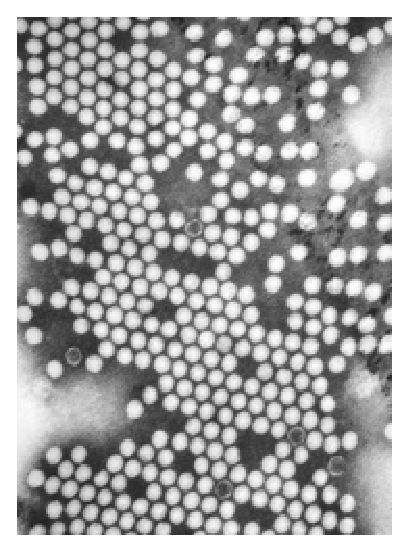
\includegraphics[width=0.25\textwidth]{../../epsimages/mm-Polio.eps}
\caption{The image of the polio virus using a transmission electron microscope.}
\label{fig:polio}
\end{center}
\end{figure}

The structure of an optical and electron microscope are compared in figure \ref{fig:p:wsl:wnm12:lvsem}. While the optical microscope uses light and focuses using lenses, the electron microscope uses electrons and focuses using electromagnets.


\begin{figure}[H]
\begin{center}
\begin{pspicture}(-1.4,-0.6)(8.4,10)
%\psgrid[gridcolor=gray]
\def\lightbulb{\pscircle(0,1){0.5}\psframe(-0.25,0)(0.25,0.5)}
\def\maglens{\psset{yunit=0.75}
\psarc(0,0){0.5}{0}{180}
\psarc(0,0){1}{0}{180}
\psframe(0.5,-0.5)(1,0)
\psframe(-1,-0.5)(-0.5,0)
\psarc(0,-0.5){0.5}{0}{180}
}
\rput(5,0){
\psline{->}(0,9)(0,0.5)
\rput(0,9){\psframe(-0.2,0)(0.2,1)}\uput[r](0.5,9.5){electron source}
\rput(0,7){\maglens}\uput[r](1,8){magnetic lens}
\psframe(-1,5.5)(1,5.7)\uput[r](1,5.6){target}
\rput(0,4){\maglens}\uput[r](1,5){objective lens}
\rput(0,2){\maglens}\uput[r](1,2){projector lens}
\psframe(-1,0)(1,1)\uput[r](1,0.5){screen}
\uput[d](0,0){electron microscope}
}

\rput(0,0){\rput{270}(0,0){\psset{unit=0.5}\eye}
\rput{180}(0,10){\lightbulb}\uput[r](0.5,9.5){light source}
\rput{90}(0,8){\psset{unit=0.7}\lens[lensGlass=true,drawing=false]} \uput[r](1,8){condenser lens}
\psframe(-1,5.5)(1,5.7)\uput[r](1,5.6){target}
\rput{90}(0,5){\psset{unit=0.5}\lens[lensGlass=true,drawing=false]} \uput[r](1,5){objective lens}
\rput{90}(0,2){\psset{unit=0.7}\lens[lensGlass=true,drawing=false]} \uput[r](1,2){eyepiece lens}
\uput[d](0,0){optical microscope}
\psline{->}(0,8.5)(0,1)
}
\end{pspicture}
\caption{Diagram of the basic components of an optical microscope and an electron microscope.}
\label{fig:p:wsl:wnm12:lvsem}
\end{center}
\end{figure}


Electron microscopes are very useful as they are able to magnify objects to a much higher resolution. This is because their de Broglie wavelengths are so much smaller than that of visible light. You hopefully remember that light is diffracted by objects which are separated by a distance of about the same size as the wavelength of the light. This diffraction then prevents you from being able to focus the transmitted light into an image. So the sizes at which diffraction occurs for a beam of electrons is much smaller than those for visible light. This is why you can magnify targets to a much higher order of magnification using electrons rather than visible light.

\begin{table}
\begin{center}
\caption{Comparison of Light and Electron Microscopes}
\begin{tabular}{|l||p{0.4\textwidth}|p{0.4\textwidth}|}\hline
& {\bf Light microscope} & {\bf Electron microscope} \\ \hline
Source & Bright lamp or laser & Electron gun \\ \hline
Radiation & U.V. or visible light & Electron beam produced by heating metal surface (e.g.\@ tungsten)\\\hline
Lenses & Curved glass surfaces & Electromagnets\\\hline
Receiver & Eye; photographic emulsion or digital image & Fluorescent screen (for location and focusing image); photographic emulsion or digital image\\\hline
Focus & Axial movement of lenses (up and down)& Adjustment of magnetic field in the electromagnets by changing the current \\\hline
Operating & Atmospheric & High vacuum\\  Pressure & &  \\ \hline
\end{tabular}
\end{center}
\end{table}

\Extension{HRTEM}{
There are High-Resolution Transmission Electron Microscopes that have been built. In fact the resolution is sufficient to show carbon atoms in diamond separated by only 89 picometres and atoms in silicon at 78 picometres. This is at magnifications of 50 million times. The ability to determine the positions of atoms within materials has made the HRTEM a very useful tool for nano-technology research. It is also important for the development of semiconductor devices for electronics and photonics.}

\Extension{SEM}{
The Scanning Electron Microscope produces images by hitting the target with a primary electron beam which then excites the surface of the target. This causes secondary electrons to be emitted from the surface which are then detected.  So the electron beam in the SEM is moved (or scanned) across the sample, while detectors build an image from the secondary electrons.

Generally, the transmission electron microscope's resolution is about an order of magnitude better than the SEM resolution. However, because the SEM image relies on surface processes rather than transmission it is able to image bulk samples (unlike optical microscopes and TEM which require the samples to be thin) and has a much greater depth of view, and so can produce images that are a good representation of the 3D structure of the sample.}

\subsection{Disadvantages of an Electron Microscope}
Electron microscopes are expensive to buy and maintain. They are also very sensitive to vibration and external magnetic fields. This means that special facilities are required to house microscopes aimed at achieving high resolutions. Also the targets have to be viewed in vacuum, as the electrons would scatter off the molecules that make up air. 

\Extension{Scanning Electron Microscope (SEM)}{
Scanning electron microscopes usually image conductive or semi-conductive materials best.  A common preparation technique is to coat the target with a several-nanometre layer of conductive material, such as gold, from a sputtering machine; however this process has the potential to disturb delicate samples.

The targets have to be prepared in many ways to give proper detail. This may result in artifacts purely as a result of the treatment. This gives the problem of distinguishing artifacts from material, particularly in biological samples. Scientists maintain that the results from various preparation techniques have been compared, and as there is no reason that they should all produce similar artifacts, it is therefore reasonable to believe that electron microscopy features correlate with living cells.}

%\begin{IFact}
%{The first electron microscope prototype was built in 1931 by the
%  German engineers Ernst Ruska and Max Knoll.
%% It was based on the ideas and discoveries of Louis de Broglie.
%  Although it was primitive and was not ideal for practical use, the instrument was still capable of magnifying objects by four hundred times. The first practical electron microscope was built at the University of Toronto in 1938, by Eli Franklin Burton and students Cecil Hall, James Hillier and Albert Prebus.
%Although modern electron microscopes can magnify objects up to two million times, they are still based upon Ruska's prototype and his correlation between wavelength and resolution. %The electron microscope is an integral part of many laboratories. Researchers use it to examine biological materials (such as microorganisms and cells), a variety of large molecules, medical biopsy samples, metals and crystalline structures, and the characteristics of various surfaces.
%}\end{IFact}

\subsection{Uses of Electron Microscopes}
Electron microscopes can be used to study:
\begin{itemize}
\item the topography of an object $-$ how its surface looks.
\item the morphology of particles making up an object  $-$ their shapes and sizes.
\item the composition of an object $-$ the elements and compounds that the object is composed of and the relative amounts of them.
\item the crystallographic information for crystalline samples $-$ how the atoms are arranged in the object.
\end{itemize}

\clearpage

\summary{VPreb}
\begin{itemize}
\item The momentum of a photon can be related to the energy of the photon, $p=\frac{E}{c}$.
\item Combined with $E=\frac{hc}{\lambda}$, a relationship between momentum and wavelength is derived.
\item De Broglie postulated that this relationship holds for all particles and any object has a de Broglie wavelength.
\end{itemize}


\begin{eocexercises}{}
\begin{enumerate}
  \item If the following particles have the same velocity, which has the shortest wavelength: electron, hydrogen atom, lead atom? 
\item A bullet weighing 30 g is fired at a velocity of $500\ems$. What is its wavelength?
\item Calculate the wavelength of an electron which has a kinetic energy of $1.602\times10^{-19}$~J.
\item If the wavelength of an electron is $10^{-9}$~m what is its velocity?
\item Considering how one calculates wavelength using slits, try to explain why we would not be able to physically observe diffraction of the cricket ball in the first worked example.
 \end{enumerate}
% Automatically inserted shortcodes - number to insert 5
\par \practiceinfo
\par \begin{tabular}[h]{cccccc}
% Question 1
(1.)	01it	&
% Question 2
(2.)	01iu	&
% Question 3
(3.)	01iv	&
% Question 4
(4.)	01iw	&
% Question 5
(5.)	01ix	&
\end{tabular}
% Automatically inserted shortcodes - number inserted 5
\end{eocexercises}


% CHILD SECTION END 



% CHILD SECTION START 


  \chapter{Electrodynamics}
\label{p:em:ed12}



\section{Introduction}
In Grade 11 you learnt how a magnetic field is generated around a current carrying conductor. You also learnt how a current is generated in a conductor that moves in a magnetic field. This chapter describes how conductors moving in a magnetic field are applied in the real-world. 

\section{Electrical machines - generators and motors}
%\begin{syllabus}
%\item Learners must be able to state that generators convert mechanical energy to electrical energy and motors convert electrical energy to mechanical energy
%\item Learners must be able to use Faraday's Law to explain why a current is induced in a coil that is rotated in a magnetic field.
%\item Learners must be able to use words and pictures to explain the basic principle of an AC generator (alternator) in which a coil is mechanically rotated in a magnetic field
%\item Learners must be able to use words and pictures to explain how a DC generator works and how it differs from an AC generator.
%\item Learners must be able to explain why a current-carrying coil placed in a magnetic field (but not parallel to the field) will turn by referring to the force exerted on moving charges by a magnetic field and the torque on the coil
%\item Learners must be able to use words and pictures to explain the basic principle of an electric motor.
%\item Learners must be able to give examples of the use of AC and DC generators.
%\item Learners must be able to give examples of the use of motors
%\end{syllabus}

We have seen that when a conductor is moved in a magnetic field or when a magnet is moved near a conductor, a current flows in the conductor. The amount of current depends on the speed at which the conductor experiences a changing magnetic field, the number of turns of the conductor and the position of the plane of the conductor with respect to the magnetic field. The effect of the orientation of the conductor with respect to the magnetic field is illustrated in Figure~\ref{fig:conductor}. 

\begin{figure}[htbp]
\begin{center}
\begin{pspicture}(0,0)(11,5)
%\psgrid[gridcolor=gray]
\def\magfieldF{\multirput(0,0)(0.25,0){9}{\psline{<-}(0,0)(0,2)}}
\def\magfieldT{\multirput(0,0)(0,0.25){9}{\multirput(0,0)(0.25,0){9}{\psdot[dotstyle=x](0,0)}}}
\def\frontview{\rput{0}{\psline[linewidth=0.1cm](1;180)(1;0)\psarc{->}{1}{0}{30}}}
\rput(0,3){\magfieldF\rput{0}(1,1){\frontview}}
\rput(0,0){\magfieldT\pscircle[linewidth=0.1cm](1,1){1}}

\rput(3,0)
{
\rput(0,3){\magfieldF\rput{45}(1,1){\frontview}}
\rput(0,0){\magfieldT\psellipse[linewidth=0.1cm](1,1)(0.5,1)}
}

\rput(6,0)
{
\rput(0,3){\magfieldF\rput{90}(1,1){\frontview}}
\rput(0,0){\magfieldT\rput(1,1){\psline[linewidth=0.1cm](1;270)(1;90)}}
}

\rput(9,0)
{
\rput(0,3){\magfieldF\rput{135}(1,1){\frontview}}
\rput(0,0){\magfieldT\psellipse[linewidth=0.1cm](1,1)(0.5,1)}
}

\uput[l](0,1){top view}
\uput[l](0,4){front view}
\rput(1,2.5){(a)}
\rput(4,2.5){(b)}
\rput(7,2.5){(c)}
\rput(10,2.5){(d)}
\end{pspicture}
\caption{Series of figures showing that the magnetic flux through a conductor is dependent on the angle that the plane of the conductor makes with the magnetic field. The greatest flux passes through the conductor when the plane of the conductor is perpendicular to the magnetic field  lines as in (a). The number of field lines passing through the conductor decreases, as the conductor rotates until it is parallel to the magnetic field (c).}
\label{fig:conductor}
\end{center}
\end{figure}

If the current flowing in the conductor were plotted as a function of the angle between the plane of the conductor and the magnetic field, then the current would vary as shown in Figure~\ref{fig:ac}. The current alternates about zero and is known as an \textit{alternating current} (abbreviated AC).


%%%% SARAH: Trying to remove the x axis numbers - they are irrelevant!
\begin{figure}[htbp]
\begin{center}
\begin{pspicture}(0,-2)(4.6,2)
%\psgrid[gridcolor=gray]
\psset{xunit=0.00556}
\psaxes[labels=none,ticks=none,dx=180,Dx=180]{<->}(0,0)(0,-1.5)(780,1.5)
\psplot{0}{720}{x sin}
\uput[r](780,0){time}
\uput[u](0,1.5){current (arbitrary units)}
\end{pspicture}
\caption{Variation of current as the angle of the plane of a conductor with the magnetic field changes.}
\label{fig:ac}
\end{center}
\end{figure}

Recall Faraday's Law which you learnt about in Grade 11:

\Definition{Faraday's Law}{The emf (electromotive force),
$\epsilon$, produced around a loop of conductor is proportional to
the rate of change of the magnetic flux, $\phi$, through the area,
$A$, of the loop. This can be stated mathematically as:
\begin{equation*}
\epsilon=-N\frac{\Delta \phi}{\Delta t}
\end {equation*}
 where $\phi=B\cdot A$ and $B$ is the strength of the magnetic field.}

Faraday's Law relates induced emf (electromotive force) to the rate of change of flux,
which is the product of the magnetic field and the cross-sectional
area the field lines pass through.
As the closed loop conductor changes orientation with respect to the magnetic field, the amount of magnetic flux through the area of the loop changes, and an emf is induced in the conducting loop. 


\subsection{Electrical generators}

\subsection*{AC generator}
The principle of rotating a conductor in a magnetic field is used in electrictrical generators. A generator converts mechanical energy (motion) into electrical energy.
 
\Definition{Generator}{A generator converts mechanical energy into electrical energy.}

The layout of a simple AC generator is shown in Figure~\ref{fig:ACgen}. The conductor in the shape of a coil is connected to a slip ring. The conductor is then manually rotated in the magnetic field generating an alternating emf. The slip rings are connected to the load via brushes.

\begin{figure}[htbp]
\begin{center}
%\begin{pspicture}(0,-2.2)(9,4)
%%\psgrid[gridcolor=gray]
%\psframe(0,2)(3,4)\uput[l](3,3){N}
%\psframe(6,2)(9,4)\uput[r](6,3){S}
%\psline[linearc=0.4cm](4.2,-1.4)(4.2,2)(3.4,2)(3.4,4)(5.6,4)(5.6,2)(4.8,2)(4.8,-0.4)
%\psframe*(4,-1)(5,-0.4)\psline(5,-0.4)(5,-1)\psline(5,-0.7)(6,-0.7)(6,0)(8,0)
%\psframe*(4,-2)(5,-1.4)\psline(5,-1.4)(5,-2)\psline(5,-1.7)(6,-1.7)(6,-2.2)(8,-2.2)
%\psframe[fillstyle=solid,fillcolor=lightgray](5,-1)(5.2,-0.4)\uput[u](5.2,-0.4){brush}
%\psframe[fillstyle=solid,fillcolor=lightgray](5,-2)(5.2,-1.4)\uput[d](5.2,-2){brush}
%\uput[l](4,-0.7){slip ring}
%\uput[l](4,-1.7){slip ring}
%\resistor[dipolestyle=zigzag](8,0)(8,-2.2){load}
%\rput(0,-1){\pscircle[linewidth=2pt](2,1){0.5}\uput[u](2,1.5){slip ring (front view)}}
%\end{pspicture}
\scalebox{1} % Change this value to rescale the drawing.
{
\begin{pspicture}(0,-3.041)(8.92,3.06)
\definecolor{color1802b}{rgb}{0.8,0.8,0.8}
\psframe[linewidth=0.042,dimen=outer](2.92,2.72)(0.04,0.86)
\psframe[linewidth=0.042,dimen=outer](8.8,2.7)(5.92,0.84)
\psbezier[linewidth=0.042](4.184828,-1.34)(4.0865517,0.88)(4.342069,0.8)(3.8310344,0.86)(3.32,0.92)(3.3396552,1.46)(3.3789656,2.14)(3.4182758,2.82)(4.08,2.68)(4.8727584,2.68)(5.6655173,2.68)(5.5,1.96)(5.5,1.48)(5.5,1.0)(5.4284515,1.0245473)(5.4,0.96)(5.371548,0.8954527)(5.0489655,0.86)(4.88,0.82)(4.7110343,0.78)(4.8334484,0.46)(4.7744827,-1.34)
\psframe[linewidth=0.042,dimen=outer,fillstyle=solid,fillcolor=black](5.06,-1.26)(3.78,-1.86)
\psframe[linewidth=0.042,dimen=outer,fillstyle=solid,fillcolor=color1802b](5.28,-1.18)(5.02,-1.92)
\psframe[linewidth=0.042,dimen=outer,fillstyle=solid,fillcolor=black](5.04,-2.36)(3.76,-2.96)
\psframe[linewidth=0.042,dimen=outer,fillstyle=solid,fillcolor=color1802b](5.26,-2.28)(5.0,-3.02)
\pscircle[linewidth=0.06,dimen=outer](1.41,-0.91){0.57}
\rput(2.5,1.765){N}
\rput(6.36,1.765){S}
\rput(5.34,-0.955){brush}
\rput(3.04,-1.595){slip ring}
\rput(3.06,-2.675){slip ring}
\rput(1.52,-0.135){slip ring (front view)}
\psline[linewidth=0.042cm,fillcolor=black](4.2,-1.82)(4.2,-2.4)
\psline[linewidth=0.042cm,fillcolor=black](5.26,-1.54)(6.04,-1.54)
\psline[linewidth=0.042cm,fillcolor=black](6.04,-1.54)(6.02,-0.84)
\psline[linewidth=0.042cm,fillcolor=black](6.02,-0.84)(7.84,-0.84)
\psline[linewidth=0.042cm,fillcolor=black](7.84,-0.84)(7.84,-1.5)
\psline[linewidth=0.042cm,fillcolor=black](7.84,-1.5)(8.08,-1.64)
\psline[linewidth=0.042cm,fillcolor=black](8.08,-1.64)(7.64,-1.8)
\psline[linewidth=0.042cm,fillcolor=black](7.64,-1.8)(8.08,-1.96)
\psline[linewidth=0.042cm,fillcolor=black](8.08,-1.96)(7.66,-2.16)
\psline[linewidth=0.042cm,fillcolor=black](7.66,-2.16)(8.08,-2.26)
\psline[linewidth=0.042cm,fillcolor=black](8.08,-2.26)(7.66,-2.46)
\psline[linewidth=0.042cm,fillcolor=black](7.66,-2.46)(7.86,-2.52)
\psline[linewidth=0.042cm,fillcolor=black](7.86,-2.52)(7.86,-3.02)
\psline[linewidth=0.042cm,fillcolor=black](7.86,-3.02)(5.96,-3.02)
\psline[linewidth=0.042cm,fillcolor=black](5.96,-3.02)(5.98,-2.64)
\psline[linewidth=0.042cm,fillcolor=black](5.98,-2.64)(5.26,-2.64)
\rput(8.57,-2.055){load}
\rput(5.11,0.545){coil}
\rput(1.47,2.905){magnet}
\rput(7.39,2.905){magnet}
\end{pspicture} 
}
\caption{Layout of an alternating current generator.}
\label{fig:ACgen}
\end{center}
\end{figure}

If a machine is constructed to rotate a magnetic field around a set of stationary wire coils with the turning of a shaft, AC voltage will be produced across the wire coils as that shaft is rotated, in accordance with Faraday's Law of electromagnetic induction. This is the basic operating principle of an AC generator.\\
 
In an AC generator the two ends of the coil are each attached to a slip ring that makes contact with brushes as the coil turns. The direction of the current changes with every half turn of the coil. As one side of the loop moves to the other pole of the magnetic field, the current in the loop changes direction. The two slip rings of the AC generator allow the coil to turn without breaking the connections to the load circuit. This type of current which changes direction is known as alternating current.\\  
 
\begin{IFact}{AC generators are also known as alternators. They are found in motor cars to charge the car battery.}
\end{IFact}

\subsection*{DC generator}
A simple DC generator is constructed the same way as an AC generator except that there is one slip ring which is split into two pieces, called a commutator, so the current in the external circuit does not change direction. The layout of a DC generator is shown in Figure~\ref{fig:DCgen}. The split-ring commutator accommodates for the change in direction of the current in the loop, thus creating direct current (DC) current going through the brushes and out to the circuit.

\begin{figure}[htbp]
\begin{center}
\begin{pspicture}(0,-2.2)(9,4)
%\psgrid[gridcolor=gray]
\psframe(0,2)(3,4)\uput[l](3,3){N}
\psframe(6,2)(9,4)\uput[r](6,3){S}
\psline[linearc=0.4cm](4.2,-0.4)(4.2,2)(3.4,2)(3.4,4)(5.6,4)(5.6,2)(4.8,2)(4.8,-0.4)
\psframe*(4,-1)(5,-0.4)\psline(5,-0.4)(5,-1)
\uput[d](4.4,-1){split ring}
\uput[ul](4,-0.4){brush}
\uput[ur](5,-0.4){brush}

\psframe[fillstyle=solid,fillcolor=lightgray](5,-1)(5.2,-0.4)\psline(5.2,-0.7)(6,-0.7)(6,0)(8,0)

\psframe[fillstyle=solid,fillcolor=lightgray](3.8,-1)(4,-0.4)\psline(3.8,-0.7)(3,-0.7)(3,-2.2)(8,-2.2)
\resistor[dipolestyle=zigzag](8,0)(8,-2.2){load}
\rput(0,-1){\psarc[linewidth=2pt](2,1){0.5}{0}{180}\psarc[linewidth=2pt](2,0.8){0.5}{180}{0}\uput[u](2,1.5){split ring commutator}}
\end{pspicture}
\caption{Layout of a direct current generator.}
\label{fig:DCgen}
\end{center}
\end{figure}

The shape of the emf from a DC generator is shown in Figure~\ref{fig:DCsignal}. The emf is not steady but is the absolute value of a sine/cosine wave.

%%% SARAH: Trying to remove x-axis numbering
\begin{figure}[htbp]
\begin{center}
\begin{pspicture}(0,-2)(4.6,2)
%\psgrid[gridcolor=gray]
\psset{xunit=0.00556}
\psaxes[labels=none,ticks=none,dx=180,Dx=180,label=0]{<->}(0,0)(0,-1.5)(780,1.5)
\def\sine{\psplot{0}{180}{x sin}}
\rput(0,0){\sine}
\rput(180,0){\sine}
\rput(360,0){\sine}
\rput(540,0){\sine}
\uput[r](780,0){$\theta$ or time}
\uput[u](0,1.5){current}
\end{pspicture}
\caption{Variation of emf in a DC generator.}
\label{fig:DCsignal}
\end{center}
\end{figure}

\subsection*{AC versus DC generators}

The problems involved with making and breaking electrical contact with a moving coil are sparking and heat, especially if the generator is turning at high speed. If the atmosphere surrounding the machine contains flammable or explosive vapors, the practical problems of spark-producing brush contacts are even greater.\\
 
If the magnetic field, rather than the coil/conductor is rotated, then brushes are not needed in an AC generator (alternator), so an alternator will not have the same problems as DC generators. 
The same benefits of AC over DC for generator design also apply to electric motors.
While DC motors need brushes to make electrical contact with moving coils of wire, AC motors do not. In fact, AC and DC motor designs are very similar to their generator counterparts. 
The AC motor is depends on the reversing magnetic field produced by alternating current through its stationary coils of wire to make the magnet rotate. The DC motor depends on the brush contacts making and breaking
connections to reverse current through the rotating coil every 1/2 rotation (180 degrees).


\subsection{Electric motors}
The basic principles of operation for a motor are the same as that of a generator, except that a motor converts electrical energy into mechanical energy (motion).

\Definition{Motor}{An electric motor converts electrical energy into mechanical energy.}

If one were to place a moving charged particle in a magnetic field, it would feel a force called the \textbf{Lorentz force}. 

\Definition{The Lorentz Force}{The Lorentz force is the force experienced by a moving charged particle in a magnetic field and can be described by:
\begin{equation*}
F = q \times v \times B
\end{equation*}
where \\
$F$ is the force (in newtons, N) \\
$q$ is the electric charge (in coulombs, C) \\
$v$ is the velocity of the charged particle (in $\rm{m.s^{-1}}$) and \\
$B$ is the magnetic field strength (in teslas, T). 
}

Current in a conductor consists of moving charges. Therefore, a current carrying coil in a magnetic field will also feel the Lorentz force. For a straight current carrying wire which is not moving:

\begin{equation*}
F = I \times L \times B
\end{equation*}
where \\
$F$ is the force (in newtons, N) \\
$I$ is the current in the wire (in amperes, A) \\
$L$ is the length of the wire which is in the magnetic field (in m) and \\
$B$ is the magnetic field strength (in teslas, T). \\

The direction of the Lorentz force is perpendicular to both the direction of the flow of current and the magnetic field and can be found using the \textbf{Right Hand Rule} as shown in the picture below. Use your \textit{right hand}; your thumb points in the direction of the current, your first finger in the direction of the magnetic field and your third finger will then point in the direction of the force.

\scalebox{1} % Change this value to rescale the drawing.
{
\begin{pspicture}(0,-2.8)(7.2617035,2.8)
\psline[linewidth=0.04cm](0.02,1.14)(1.42,1.14)
\psline[linewidth=0.04cm](1.42,1.14)(1.42,-0.84)
\psline[linewidth=0.04cm](1.42,-0.84)(0.0,-0.84)
\psline[linewidth=0.04cm](7.2182946,-0.8211864)(5.818297,-0.8187762)
\psline[linewidth=0.04cm](5.818297,-0.8187762)(5.8217053,1.1612209)
\psline[linewidth=0.04cm](5.8217053,1.1612209)(7.2417035,1.1587762)
\rput(1.14,0.125){S}
\rput(6.14,0.165){N}
\pscircle[linewidth=0.04,dimen=outer](4.07,0.13){0.21}
\pscircle[linewidth=0.04,dimen=outer](4.21,0.05){0.01}
\rput(4.08,0.105){+}
\psline[linewidth=0.054cm,arrowsize=0.05291667cm 2.0,arrowlength=1.4,arrowinset=0.4]{->}(3.96,-0.02)(2.26,-2.24)
\psline[linewidth=0.054cm,arrowsize=0.05291667cm 2.0,arrowlength=1.4,arrowinset=0.4]{->}(3.9,0.18)(1.5,0.18)
\psline[linewidth=0.054cm,arrowsize=0.05291667cm 2.0,arrowlength=1.4,arrowinset=0.4]{->}(4.06,0.32)(4.06,2.7)
\rput(0.63,1.345){magnet}
\rput(6.53,1.365){magnet}
\rput(5.65,2.625){\small Direction of current }
\rput(4.98,2.305){\small in the wire}
\rput(4.89,1.94){\footnotesize [THUMB]}
\rput(3.41,-2.58){\footnotesize [2nd FINGER]}
\rput(4.63,-2.195){\small Direction of the Lorentz force}
\rput(2.65,0.765){\small Direction of the }
\rput(2.58,0.445){\small magnetic field}
\rput(2.43,-0.18){\footnotesize [1st FINGER]}
\end{pspicture} 
}

Both motors and generators can be explained in terms of a coil that rotates in a magnetic field. In a generator the coil is attached to an external circuit that is turned, resulting in a changing flux that induces an emf. In a motor, a current-carrying coil in a magnetic field experiences a force on both sides of the coil, creating a twisting force (called a \textit{torque}, pronounce like 'talk') which makes it turn.\\

Any coil carrying current can feel a force in a magnetic field. The force is the Lorentz force on the moving charges in the conductor. The force on opposite sides of the coil will be in opposite directions because the charges are moving in opposite directions. This means the coil will rotate, see the picture below:

\begin{center}
\scalebox{1} % Change this value to rescale the drawing.
{
\begin{pspicture}(0,-2.32)(7.96,2.32)
\definecolor{color0}{rgb}{0.6,0.6,0.6}
\psline[linewidth=0.04cm,linecolor=color0,arrowsize=0.05291667cm 4.0,arrowlength=1.4,arrowinset=0.4]{->}(0.9,1.94)(0.9,-1.74)
\psline[linewidth=0.04cm,linecolor=color0,arrowsize=0.05291667cm 4.0,arrowlength=1.4,arrowinset=0.4]{->}(1.5,1.94)(1.5,-1.74)
\psline[linewidth=0.04cm,linecolor=color0,arrowsize=0.05291667cm 4.0,arrowlength=1.4,arrowinset=0.4]{->}(2.12,1.92)(2.12,-1.76)
\psline[linewidth=0.04cm,linecolor=color0,arrowsize=0.05291667cm 4.0,arrowlength=1.4,arrowinset=0.4]{->}(2.72,1.94)(2.72,-1.74)
\psline[linewidth=0.04cm,linecolor=color0,arrowsize=0.05291667cm 4.0,arrowlength=1.4,arrowinset=0.4]{->}(3.32,1.92)(3.32,-1.76)
\psline[linewidth=0.04cm,linecolor=color0,arrowsize=0.05291667cm 4.0,arrowlength=1.4,arrowinset=0.4]{->}(3.92,1.92)(3.92,-1.76)
\psline[linewidth=0.04cm,linecolor=color0,arrowsize=0.05291667cm 4.0,arrowlength=1.4,arrowinset=0.4]{->}(4.5,1.92)(4.5,-1.76)
\psline[linewidth=0.04cm,linecolor=color0,arrowsize=0.05291667cm 4.0,arrowlength=1.4,arrowinset=0.4]{->}(5.12,1.94)(5.12,-1.74)
\psline[linewidth=0.04cm,linecolor=color0,arrowsize=0.05291667cm 4.0,arrowlength=1.4,arrowinset=0.4]{->}(5.72,1.94)(5.72,-1.74)
\psline[linewidth=0.04cm,linecolor=color0,arrowsize=0.05291667cm 4.0,arrowlength=1.4,arrowinset=0.4]{->}(6.32,1.94)(6.32,-1.74)
\psline[linewidth=0.04](0.34,0.22)(1.88,0.22)(2.26,1.16)(6.16,1.16)(5.64,-1.1)(1.42,-1.08)(1.76,0.0)(0.24,0.0)
\psellipse[linewidth=0.04,linecolor=color0,dimen=outer](6.99,0.16)(0.39,1.0)
\psbezier[linewidth=0.04,arrowsize=0.05291667cm 4.0,arrowlength=1.4,arrowinset=0.4]{->}(7.34,0.04)(7.36,0.06)(7.3,-0.86)(7.0142856,-0.82)(6.7285714,-0.78)(6.614286,-0.33518797)(6.6714287,0.46)(6.7285714,1.255188)(7.16,1.32)(7.36,0.54)
\psline[linewidth=0.04cm,arrowsize=0.05291667cm 3.0,arrowlength=1.4,arrowinset=0.4]{->}(3.46,1.16)(4.66,1.16)
\psline[linewidth=0.04cm,arrowsize=0.05291667cm 3.0,arrowlength=1.4,arrowinset=0.4]{->}(4.7,-1.1)(3.5,-1.1)
\psframe[linewidth=0.02,linecolor=color0,dimen=outer](2.96,0.38)(2.74,0.14)
\psline[linewidth=0.12cm,arrowsize=0.05291667cm 2.0,arrowlength=1.4,arrowinset=0.4]{->}(4.02,1.14)(4.76,1.62)
\psline[linewidth=0.12cm,arrowsize=0.05291667cm 2.0,arrowlength=1.4,arrowinset=0.4]{->}(3.32,-1.08)(2.68,-1.62)
\psline[linewidth=0.12cm,arrowsize=0.05291667cm 2.0,arrowlength=1.4,arrowinset=0.4]{->}(2.1,0.66)(1.56,0.66)
\psline[linewidth=0.12cm,arrowsize=0.05291667cm 2.0,arrowlength=1.4,arrowinset=0.4]{->}(1.6,-0.62)(1.06,-0.62)
\psline[linewidth=0.12cm,arrowsize=0.05291667cm 2.0,arrowlength=1.4,arrowinset=0.4]{->}(6.02,0.66)(6.56,0.66)
\psline[linewidth=0.12cm,arrowsize=0.05291667cm 2.0,arrowlength=1.4,arrowinset=0.4]{->}(5.7,-0.64)(6.24,-0.64)
\rput(5.12,2.125){resultant force is \textit{into} the page}
\rput(2.95,-2.095){resultant force is \textit{out of} the page}
\psline[linewidth=0.02cm](0.04,0.14)(7.72,0.14)
\end{pspicture} 
}

\end{center}

 
Instead of rotating the loops through a magnetic field to create electricity, a current is sent through the wires, creating electromagnets. The outer magnets will then repel the electromagnets and rotate the shaft as an electric motor. If the current is AC, the two slip rings are required to create an AC motor. An AC motor is shown in Figure~\ref{fig:ACmotor} 

\begin{figure}[H]
\begin{center}
%\begin{pspicture}(0,-2.2)(9,4)
%%\psgrid[gridcolor=gray]
%\psframe(0,2)(3,4)\uput[l](3,3){N}
%\psframe(6,2)(9,4)\uput[r](6,3){S}
%\psline[linearc=0.4cm](4.2,-1.4)(4.2,2)(3.4,2)(3.4,4)(5.6,4)(5.6,2)(4.8,2)(4.8,-0.4)
%\psframe*(4,-1)(5,-0.4)\psline(5,-0.4)(5,-1)\psline(5,-0.7)(6,-0.7)(6,0)(8,0)
%\psframe*(4,-2)(5,-1.4)\psline(5,-1.4)(5,-2)\psline(5,-1.7)(6,-1.7)(6,-2.2)(8,-2.2)
%\psframe[fillstyle=solid,fillcolor=lightgray](5,-1)(5.2,-0.4)\uput[u](5.2,-0.4){brush}
%\psframe[fillstyle=solid,fillcolor=lightgray](5,-2)(5.2,-1.4)\uput[d](5.2,-2){brush}
%\uput[l](4,-0.7){slip ring}
%\uput[l](4,-1.7){slip ring}
%\battery(8,0)(8,-2.2){}
%\rput(0,-1){\pscircle[linewidth=2pt](2,1){0.5}\uput[u](2,1.5){slip ring (front view)}}
%\end{pspicture}
\scalebox{1} % Change this value to rescale the drawing.
{
\begin{pspicture}(0,-3.041)(8.8,3.06)
\definecolor{color1802b}{rgb}{0.8,0.8,0.8}
\psframe[linewidth=0.042,dimen=outer](2.92,2.72)(0.04,0.86)
\psframe[linewidth=0.042,dimen=outer](8.8,2.7)(5.92,0.84)
\psbezier[linewidth=0.042](4.184828,-1.34)(4.0865517,0.88)(4.342069,0.8)(3.8310344,0.86)(3.32,0.92)(3.3396552,1.46)(3.3789656,2.14)(3.4182758,2.82)(4.08,2.68)(4.8727584,2.68)(5.6655173,2.68)(5.5,1.96)(5.5,1.48)(5.5,1.0)(5.4284515,1.0245473)(5.4,0.96)(5.371548,0.8954527)(5.0489655,0.86)(4.88,0.82)(4.7110343,0.78)(4.8334484,0.46)(4.7744827,-1.34)
\psframe[linewidth=0.042,dimen=outer,fillstyle=solid,fillcolor=black](5.06,-1.26)(3.78,-1.86)
\psframe[linewidth=0.042,dimen=outer,fillstyle=solid,fillcolor=color1802b](5.28,-1.18)(5.02,-1.92)
\psframe[linewidth=0.042,dimen=outer,fillstyle=solid,fillcolor=black](5.04,-2.36)(3.76,-2.96)
\psframe[linewidth=0.042,dimen=outer,fillstyle=solid,fillcolor=color1802b](5.26,-2.28)(5.0,-3.02)
\pscircle[linewidth=0.06,dimen=outer](1.41,-0.91){0.57}
\rput(2.5,1.765){N}
\rput(6.36,1.765){S}
\rput(5.34,-0.955){brush}
\rput(3.04,-1.595){slip ring}
\rput(3.06,-2.675){slip ring}
\rput(1.52,-0.135){slip ring (front view)}
\psline[linewidth=0.042cm,fillcolor=black](4.2,-1.82)(4.2,-2.4)
\psline[linewidth=0.042cm,fillcolor=black](5.26,-1.54)(6.04,-1.54)
\psline[linewidth=0.042cm,fillcolor=black](6.04,-1.54)(6.02,-0.84)
\psline[linewidth=0.042cm,fillcolor=black](6.02,-0.84)(7.84,-0.84)
\psline[linewidth=0.042cm,fillcolor=black](7.84,-0.84)(7.84,-1.5)
\psline[linewidth=0.042cm,fillcolor=black](7.86,-2.52)(7.86,-3.02)
\psline[linewidth=0.042cm,fillcolor=black](7.86,-3.02)(5.96,-3.02)
\psline[linewidth=0.042cm,fillcolor=black](5.96,-3.02)(5.98,-2.64)
\psline[linewidth=0.042cm,fillcolor=black](5.98,-2.64)(5.26,-2.64)
\rput(5.11,0.545){coil}
\rput(1.47,2.905){magnet}
\rput(7.39,2.905){magnet}
\psframe[linewidth=0.042,dimen=outer](8.68,-1.52)(7.62,-2.54)
\rput(8.11,-1.855){\scriptsize AC}
\rput(8.16,-2.095){\scriptsize source}
\end{pspicture} 
}
\caption{Layout of an alternating current motor.}
\label{fig:ACmotor}
\end{center}
\end{figure}

If the current is DC, split-ring commutators are required to create a DC motor. This is shown in Figure~\ref{fig:DCmotor}.

\begin{figure}[H]
\begin{center}
\begin{pspicture}(0,-2.2)(9,4)
%\psgrid[gridcolor=gray]
\psframe(0,2)(3,4)\uput[l](3,3){N}
\psframe(6,2)(9,4)\uput[r](6,3){S}
\psline[linearc=0.4cm](4.2,-0.4)(4.2,2)(3.4,2)(3.4,4)(5.6,4)(5.6,2)(4.8,2)(4.8,-0.4)
\psframe*(4,-1)(5,-0.4)\psline(5,-0.4)(5,-1)
\uput[d](4.4,-1){split ring}
\uput[ul](4,-0.4){brush}
\uput[ur](5,-0.4){brush}

\psframe[fillstyle=solid,fillcolor=lightgray](5,-1)(5.2,-0.4)\psline(5.2,-0.7)(6,-0.7)(6,0)(8,0)

\psframe[fillstyle=solid,fillcolor=lightgray](3.8,-1)(4,-0.4)\psline(3.8,-0.7)(3,-0.7)(3,-2.2)(8,-2.2)
\battery(8,0)(8,-2.2){}
\rput(0,-1){\psarc[linewidth=2pt](2,1){0.5}{0}{180}\psarc[linewidth=2pt](2,0.8){0.5}{180}{0}\uput[u](2,1.5){split ring commutator}}
\end{pspicture}
\caption{Layout of a direct current motor.}
\label{fig:DCmotor}
\end{center}
\end{figure}


\subsection{Real-life applications}

\subsubsection{Cars}
A car contains an alternator that charges its battery and powers the car's electric system when its engine is running. Alternators have the great advantage over direct-current generators of not using a commutator, which makes them simpler, lighter, less costly, and more rugged than a DC generator.

\Activity{Research Topic}{Alternators}
{Try to find out the different ampere values produced by alternators for different types of machines. Compare these to understand what numbers make sense in the real world. You will find different numbers for cars, trucks, buses, boats etc. Try to find out what other machines might have alternators.
}

A car also contains a DC electric motor, the starter motor, to turn over the engine to start it.
A starter motor consists of the very powerful DC electric motor and starter solenoid that is attached to the motor.
A starter motor requires a very high current to crank the engine, that's why it's connected to the battery with large cables. 

\subsubsection{Electricity Generation}

AC generators are mainly used in the real-world to generate electricity.\\
 
\begin{figure}[htbp]
\begin{center}
\begin{pspicture}(-5,-3)(5,3)
%\psgrid
\rput(0,0){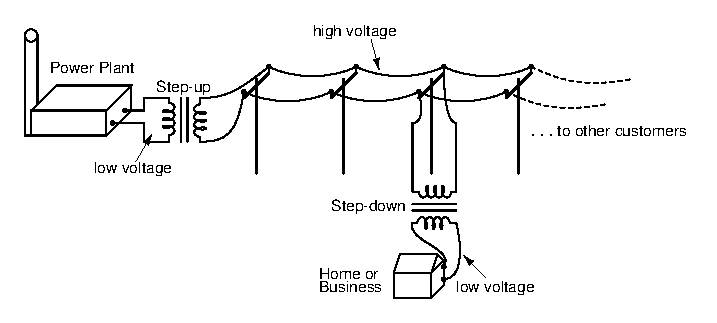
\includegraphics{../../epsimages/02007.eps}}
\end{pspicture}
\caption{AC generators are used at the power plant to generate electricity.}
\end{center}
\end{figure}

\subsection {Exercise - generators and motors}
\begin{enumerate}
\item State the difference between a generator and a motor.
\item Use Faraday's Law to explain why a current is induced in a coil that is rotated in a magnetic field.
\item Explain the basic principle of an AC generator in which a coil is mechanically rotated in a magnetic field. Draw a diagram to support your answer.
\item  Explain how a DC generator works. Draw a diagram to support your answer. Also, describe how a DC generator differs from an AC generator.
\item  Explain why a current-carrying coil placed in a magnetic field (but not parallel to the field) will turn. Refer to the force exerted on moving charges by a magnetic field and the torque on the coil.
\item  Explain the basic principle of an electric motor. Draw a diagram to support your answer.
\item  Give examples of the use of AC and DC generators.
\item  Give examples of the uses of motors.
\end{enumerate}

\section{Alternating Current}
%\begin{syllabus}
%\item Learners must be able to Explain the advantages of alternating current
%\item Learners must be able to Write expressions for the current and voltage in an AC circuit
%\item Learners must be able to Define the rms (root mean square) values for current and voltage as Irms.  =   and Vrms.  =  respectively, and explain why these values are useful.
%\item Learners must be able to Draw a graph of voltage vs time and current vs time for an AC circuit.
%\item Note: The main advantage to AC is that the voltage can be changed using transformers.  That means that the voltage can be stepped up at power stations to a very high voltage so that electrical energy can be transmitted along power lines at low current and therefore experience low energy loss due to heating.  The voltage can then be stepped down for use in buildings, street lights, and so forth.
%\end{syllabus}

Most students learning about electricity begin with what is known as \textit{direct current} (DC), which is electricity flowing in a constant direction. DC is the kind of electricity made by a battery, with definite positive and negative terminals.\\ 
 
However, we have seen that the electricity produced by some generators alternates and is therefore known as \textit{alternating current} (AC). The main advantage to AC is that the voltage can be changed using transformers.  That means that the voltage can be stepped up at power stations to a very high voltage so that electrical energy can be transmitted along power lines at low current and therefore experience low energy loss due to heating.  The voltage can then be stepped down for use in buildings and street lights.

\begin{IFact}{In South Africa alternating current is generated at a frequency of 50~Hz.}\end{IFact}

The circuit symbol for alternating current is:
\begin{center}
\begin{pspicture}(0,0)(2,2)
\Ucc[labeloffset=0](0,1)(2,1){\Huge $\sim$}
\end{pspicture}
\end{center}

Graphs of voltage against time and current against time for an AC circuit are shown in Figure~\ref{fig:ACgraphs}

%%% SARAH: Get rid of the numbering on the x axis!!!
\begin{figure}[htbp]
\begin{center}
\begin{pspicture}(0,-2)(4.6,2)
%\psgrid[gridcolor=gray]
\psset{xunit=0.00556}
\psaxes[labels=none,ticks=none,dx=180,Dx=180]{<->}(0,0)(0,-1.5)(780,1.5)
\psplot{0}{720}{x sin}
\uput[r](780,0){time}
\uput[u](0,1.5){current OR voltage}
\end{pspicture}
\caption{Graph of current or voltage in an AC circuit.}
\label{fig:ACgraphs}
\end{center}
\end{figure}

In an ideal DC circuit the current and voltage are constant. In an AC circuit the current and voltage vary with time. The value of the current or voltage at any specific time is called the \textit{instantaneous current or voltage} and is calculated as follows:
\begin{eqnarray*}
i&=&I_{max}\sin(2\pi f t + \phi)\\
v&=&V_{max}\sin(2\pi f t)
\end{eqnarray*}\\
 
$i$ is the instantaneous current. $I_{max}$ is the maximum current. $v$ is the instantaneous voltage. $V_{max}$ is the maximum voltage. $f$ is the frequency of the AC and $t$ is the time at which the instantaneous current or voltage is being calculated.\\
The average value we use for AC is known as the root mean square (rms) average. This is defined as:
\begin{eqnarray*}
I_{rms}&=&\frac{I_{max}}{\sqrt{2}}\\
V_{rms}&=&\frac{V_{max}}{\sqrt{2}}
\end{eqnarray*}\\
Since AC varies sinusoidally, with as much positive as negative, doing a straight average would get you zero for the average voltage. The rms value by-passes this problem.

\subsection {Exercise - alternating  current}
\begin{enumerate}
\item Explain the advantages of alternating current.
\item Write expressions for the current and voltage in an AC circuit.
\item Define the rms (root mean square) values for current and voltage for AC.
\item What is the period of the AC generated in South Africa?
\item If $V_{max}$ at a power station generator is 340~V AC, what is the mains supply (rms voltage) in our household?
\item Draw a graph of voltage vs time and current vs time for an AC circuit.
\end{enumerate}

\section{Capacitance and inductance}
%\begin{syllabus}
%\item The learner must be able to Revise capacitance from Grade 11
%\item The learner must be able to Define the reactance of a capacitor as $X_C=\frac{1}{2\pi fC}$  where reactance in an AC circuit plays a similar role to resistance in a DC circuit
%\item The learner must be able to Explain that a capacitor blocks the flow of DC and low frequency AC but allows the flow of high frequency AC because its reactance decreases with increasing frequency.
%\item The learner must be able to Describe an inductor as a solenoid, and inductance, L, as the ability of the solenoid to create an induced voltage when a changing current passes through it
%\item The learner must be able to Define the reactance of an inductor as $X_L = 2\pi fL$
%\item The learner must be able to Calculate the inductance of a solenoid using the expression $L=\frac{\mu_0 A N^2}{l}$, where inductance is measured in henry (H).
%\item The learner must be able to Explain that an inductor blocks high frequency AC because its reactance increases with frequency, but allows low frequency AC and DC to pass.
%\end{syllabus}

Capacitors and inductors are found in many circuits. Capacitors store an electric field, and are used as temporary power sources as well as to minimize power fluctuations in major circuits. Inductors work in conjunction with capacitors for electrical signal processing. Here we explain the physics and applications of both.

\subsection{Capacitance}
You have learnt about capacitance and capacitors in Grade 11. %Please read through Chapter~\ref{p:em:es11:c} to recap what you learnt about capacitance in a DC circuit.\\ 
 
In this section you will learn about capacitance in an AC circuit. A capacitor in an AC circuit has \textit{reactance}. Reactance in an AC circuit plays a similar role to resistance in a DC circuit. The reactance of a capacitor $X_C$ is defined as:\\
\begin{equation*}
X_C=\frac{1}{2\pi fC}
\end{equation*}
where $C$ is the capacitance and $f$ is the AC frequency.\\
 
If we examine the equation for the reactance of a capacitor, we see that the frequency is in the denominator. Therefore, when the frequency is low, the capacitive reactance is very high. This is why a capacitor blocks the flow of DC and low frequency AC because its reactance increases with decreasing frequency.\\ 
 
When the frequency is high, the capacitive reactance is low. This is why a capacitor allows the flow of high frequency AC because its reactance decreases with increasing frequency.


\subsection{Inductance}

Inductance (measured in henries, symbol H) is a measure of the generated emf for a unit change in current. For example, an inductor with an inductance of 1~H produces an emf of 1~V when the current through the inductor changes at the rate of 1~A$\cdot$s$^{-1}$.\\ 

An inductor is a passive electrical device used in electrical circuits for its property of inductance. An inductor is usually made as a coil (or solenoid) of conducting material, typically copper wire, wrapped around a core either of air or of ferromagnetic material.\\ 
 
Electrical current through the conductor creates a magnetic flux proportional to the current. A change in this current creates a change in magnetic flux that, in turn, generates an emf that acts to oppose this change in current.\\ 

 
The inductance of an inductor is determined by several factors:
\begin{itemize}
\item the shape of the coil; a short, fat coil has a higher inductance than one that is thin and tall.
\item the material that the conductor is wrapped around. 
\item how the conductor is wound; winding in opposite directions will cancel out the inductance effect, and you will have only a resistor.
\end{itemize}

The inductance of a solenoid is defined by:\\
 \begin{equation*}
L=\frac{\mu_0 A N^2}{l}
 \end{equation*}
where $\mu_0$ is the permeability of the core material (in this case air), $A$ is the cross-sectional area of the solenoid, $N$ is the number of turns and $l$ is the length of the solenoid. 

\Definition{Permeability}{Permeability is the property of a material which describes the magnetisation developed in that material when excited by a source.}

\begin{IFact}{The permeability of free space is $4 \pi \times 10^{-7}$ henry per metre.}
\end{IFact}

\begin{wex}{Inductance I}{Determine the inductance of a coil with a core material of air. A cross-sectional area of $0,3\rm{m^2}$, with 1000 turns and a length of 0,1~m}
{
\westep{Determine how to approach the problem}
We are calculating inductance, so we use the equation:
\begin{eqnarray*}
L=\frac{\mu_0 A N^2}{l}\\
\end{eqnarray*}\\
The permeability is that for free space:$4 \pi \textrm{x} 10^{-7}$ henry per metre.

\westep{Solve the problem}
\begin{eqnarray*}
L&=&\frac{\mu_0 A N^2}{l}\\
&=&\frac{(4 \pi \times 10^{-7})(0,3)(1000)}{0,1}\\ 
&=&3,8 \times 10^{-3} \textrm H/m\\
\end{eqnarray*}

\westep{Write the final answer}
The inductance of the coil is $3,8\times 10^{-3}$~H/m.}
\end{wex}

\begin{wex}{Inductance II}{Calculate the inductance of a 5~cm long solenoid with a diameter of 4~mm and 2000 turns.
}
{Again this is an inductance problem, so we use the same formula as the worked example above.\\
 
$$\textrm{r} = \frac{4 \textrm{ mm}}{2} = 2 \textrm{ mm} = 0,002 \textrm{ m}$$
$$\textrm{A} = \pi \textrm{r}^2 = \pi \times 0,002^2$$

\begin{eqnarray*}
\textrm{L} & = & \frac{\mu_0 \textrm{A} \textrm{N}^2}{l}\\
& = & \frac{4 \pi \times 10^{-7} \times 0,002^2 \times \pi \times 2000^2}{0,05}\\
& = & 0,00126 \textrm{ H}\\
& = & 1,26\textrm{ mH}\\
\end{eqnarray*}
}

\end{wex}

An inductor in an AC circuit also has a reactance, $X_L$. Reactance is the property of an inductor that opposes the flow of AC current. Reactance is defined by:

\begin{equation*}
X_L = 2\pi fL
\end{equation*}
 
where $L$ is the inductance and $f$ is the frequency of the AC.\\
 
If we examine the equation for the reactance of an inductor, we see that inductive reactance increases with increasing frequency. Therefore, when the frequency is low, the inductive reactance is very low. This is why an inductor allows the flow of DC and low frequency AC because its reactance decreases with decreasing frequency.\\ 
 
When the frequency is high, the inductive reactance is high. This is why an inductor blocks the flow of high frequency AC because its reactance increases with increasing frequency.

\subsection {Exercise - capacitance and inductance}
\begin{enumerate}
\item Describe what is meant by reactance.
\item Define the reactance of a capacitor.
\item Explain how a capacitor blocks the flow of DC and low frequency AC but allows the flow of high frequency AC.
\item Describe what is an inductor.
\item Describe what is inductance.
\item What is the unit of inductance?
\item Define the reactance of an inductor.
\item Write the equation describing the inductance of a solenoid.
\item Explain how an inductor blocks high frequency AC, but allows low frequency AC and DC to pass.
\end{enumerate}

\summary{aaa}
\begin{enumerate}
\item Electrical generators convert mechanical energy into electrical energy.
\item Electric motors convert electrical energy into mechanical energy.
\item There are two types of generators - AC and DC. An AC generator is also called an alternator.
\item There are two types of motors - AC and DC.
\item Alternating current (AC) has many advantages over direct current (DC).
\item Capacitors and inductors are important components in an AC circuit.
\item The reactance of a capacitor or inductor is affected by the frequency of the AC.
\end{enumerate}

\begin{eocexercises}{}
\begin{enumerate}
\item{[SC 2003/11] Explain the difference between alternating current (AC) and direct current (DC).}

\item Explain how an AC generator works. You may use sketches to support your answer.

\item What are the advantages of using an AC motor rather than a DC motor.

\item Explain how a DC motor works.
 
\item At what frequency is AC generated by Eskom in South Africa?

\item [IEB 2001/11 HG1] - \textbf{Work, Energy and Power in Electric Circuits}\\
Mr. Smith read through the agreement with Eskom (the electricity provider). He found out that alternating current is supplied to his house at a frequency of 50 Hz. He then consulted a book on electric current, and discovered that alternating current moves to and fro in the conductor. So he refused to pay his Eskom bill on the grounds that every electron that entered his house would leave his house again, so therefore Eskom had supplied him with nothing!\\
 
Was Mr. Smith correct? Or has he misunderstood something about what he is paying for? Explain your answer briefly.
 

\item What do we mean by the following terms in electrodynamics?
\begin{enumerate}
\item inductance
\item reactance
\item solenoid
\item permeability

\end{enumerate}

\end{enumerate}


% Automatically inserted shortcodes - number to insert 7
\par \practiceinfo
\par \begin{tabular}[h]{cccccc}
% Question 1
(1.)	01iy	&
% Question 2
(2.)	01iz	&
% Question 3
(3.)	01j0	&
% Question 4
(4.)	01j1	&
% Question 5
(5.)	01j2	&
% Question 6
(6.)	01j3	\\ % End row of shortcodes
% Question 7
(7.)	01j4	&
\end{tabular}
% Automatically inserted shortcodes - number inserted 7
\end{eocexercises}

% CHILD SECTION END 



% CHILD SECTION START 

\setlength{\parskip}{2ex}


  \chapter{Electronics}
\label{p:em:el12}

%\nts{Status: Ready for evaulation.  Dynamic references need adding where previous chapters are referred to.}

\section{Introduction}
Electronics and electrical devices surround us in daily life. From the street lights and water pumps to computers and digital phones, electronics have enabled the digital revolution to occur. All electronics are built on a backbone of simple circuits, and so an understanding of circuits is vital in understanding more complex devices.

This chapter will explain the basic physics principles of many of the components of electronic devices.  We will begin with an explanation of capacitors and inductors. We see how these are used in tuning a radio.  Next, we look at {\bf active} components such as transistors and operational amplifiers. Lastly, the chapter will finish with an explanation of digital electronics, including logic gates and counting circuits. 

Before studying this chapter, you will want to remind yourself of:
\begin{itemize}
%\item The meaning of voltage ($V$), current ($I$) and resistance ($R$), as covered in Grade 10 (see chapter~\ref{p:ElecCircuitsG10}), and Grade 11 (see chapter~\ref{p:em:ec11}).
\item The meaning of voltage ($V$), current ($I$) and resistance ($R$), as covered in Grade 10, and Grade 11.
\item Capacitors in electric circuits, as covered in Grade 11 (see section 17.6).
\item Semiconductors, as covered in Grade 11 (see chapter 20).
\item The meaning of an alternating current (see section 28.3).
\item Capacitance ($C$) and Inductance ($L$) (see section 28.4).
\end{itemize}
%\nts{Dynamic references need to be put in place to direct the reader to the other chapters.}
\chapterstartvideo{VPpml}
\section{Capacitive and Inductive Circuits}
%\begin{syllabus}
%\item The learner must be able to Perform calculations on capacitive circuits using the formula:	$V^2  =  I^2(R^2 + X_C^2)$
%\item The learner must be able to Understand that in a circuit containing both resistive and reactive components, the ratio $\frac{V}{I}$ is neither pure resistance nor pure reactance.  The ratio is called impedance, $Z$, where $Z  = \sqrt{R^2+X_C^2}$ and is measured in $\Omega$ s.
%\item The learner must be able to Understand that any coil has inductance, but also resistance.  So a coil can be considered as a resistance and an inductance in series.  The impedance of an inductor is given by: $Z  = \sqrt{R^2+X_L^2}$
%\end{syllabus}

Earlier in Grade 12, you were shown alternating currents (AC) and you saw that the voltage and the current varied with time.  If the AC supply is connected to a resistor, then the current and voltage will be proportional to each other.  This means that the current and voltage will `peak' at the same time.  We say that the current and voltage are {\bf in phase}.  This is shown in Figure~\ref{fig:VIres}.

\begin{figure}[htbp]
\begin{center}
\begin{pspicture}(0,-2.5)(10,3)
\psline[arrows=->](0,0)(9,0)
\uput[r](8.5,-0.5){Time}
\psplot[xunit=0.0111,%
		plotstyle=curve]%
		{0}{720}{x sin}
\psplot[xunit=0.0111,%
		plotstyle=curve,%
		linestyle=dashed]%
		{0}{720}{x sin 2 mul}
\uput[r](1.1,2){Current}
\uput[r](1.1,1){Voltage}
\end{pspicture}
\caption{The voltage and current are in phase when a resistor is connected to an alternating voltage.}
\label{fig:VIres}
\end{center}
\end{figure}

When a capacitor is connected to an alternating voltage, the maximum voltage is proportional to the maximum current, but the maximum voltage does not occur at the same time as the maximum current.  The current has its maximum (it peaks) one quarter of a cycle before the voltage peaks.  Engineers say that the `current leads the voltage by $90^{\circ}$'.  This is shown in Figure~\ref{fig:VIcap}.

\begin{figure}[htbp]
\begin{center}
\begin{pspicture}(0,-2.5)(10,3)
\psline[arrows=->](0,0)(9,0)
\uput[r](8.5,-0.5){Time}
\psplot[xunit=0.0111,%
		plotstyle=curve]%
		{0}{720}{x sin}
\psplot[xunit=0.0111,%
		plotstyle=curve,%
		linestyle=dashed]%
		{0}{720}{x 90 add sin 2 mul}
\uput[r](0.1,2){Current}
\uput[r](1.1,1){Voltage}
\end{pspicture}
\caption{The current peaks (has its maximum) one quarter of a wave before the voltage when a capacitor is connected to an alternating voltage.}
\label{fig:VIcap}
\end{center}
\end{figure}

For a circuit with a capacitor, the instantaneous value of $\frac{V}{I}$ is not constant.  However, the value of $\frac{V_{\mathrm{max}}}{I_{\mathrm{max}}}$ is useful, and is called the {\bf capacitive reactance} ($X_{C}$) of the component.  Because it is still a voltage divided by a current (like resistance), its unit is the ohm.  The value of $X_{C}$ ($C$ standing for capacitor) depends on its capacitance ($C$) and the frequency ($f$) of the alternating current (in South Africa 50 Hz).

\equ{X_{C} = \frac{V_{\mathrm{max}}}{I_{\mathrm{max}}} = \frac{1}{2 \pi f C}}{eq:xc}

Inductors are very similar, but the current peaks $90^{\circ}$ after the voltage.  This is shown in Figure~\ref{fig:VIind}.  Engineers say that the `current lags the voltage'.  Again, the ratio of maximum voltage to maximum current is called the reactance --- this time inductive reactance ($X_{L}$).  The value of the reactance depends on its inductance ($L$).

\equ{X_{L} = \frac{V_{\mathrm{max}}}{I_{\mathrm{max}}} = 2 \pi f L}{eq:xl}

\begin{figure}[htbp]
\begin{center}
\begin{pspicture}(0,-2)(10,3)
\psline[arrows=->](0,0)(9,0)
\uput[r](8.5,-0.5){Time}
\psplot[xunit=0.0111,%
		plotstyle=curve]%
		{0}{720}{x sin}
\psplot[xunit=0.0111,%
		plotstyle=curve,%
		linestyle=dashed]%
		{0}{720}{x 90 sub sin 2 mul}
\uput[r](2.1,2){Current}
\uput[r](1.1,1){Voltage}
\end{pspicture}
\caption{The current peaks (has its maximum) one quarter of a wave after the voltage when an inductor is connected to an alternating voltage.}
\label{fig:VIind}
\end{center}
\end{figure}

\Definition{Reactance}{The ratio of the maximum voltage to the maximum current when a capacitor or inductor is connected to an alternating voltage.  The unit of reactance is the ohm.}

While inductive and capacitive reactances are similar, in one sense they are opposites.  For an inductor, the current peaks $90^{\circ}$ {\bf after} the voltage.  For a capacitor the current peaks $90^{\circ}$ {\bf ahead} of the voltage.  When we work out the total reactance for an inductor and a capacitor in series, we use the formula
\equ{X_{\mathrm{total}} = X_{L} - X_{C}}{eq:xtotal}

to take this into account.  This formula can also be used when there is more than one inductor or more than one capacitor in the circuit.  The total reactance is the sum of all of the inductive reactances minus the sum of all the capacitive reactances.  The magnitude (number) in the final result gives the ratio of maximum voltage to maximum current in the circuit as a whole.  The sign of the final result tells you its phase.  If it is positive, the current peaks $90^{\circ}$ after the voltage, if it is negative, the current peaks $90^{\circ}$ before the voltage.


If a series circuit contains resistors as well, then the situation is more complicated.  The maximum current is still proportional to the maximum voltage, but the phase difference between them won't be $90^{\circ}$.  The ratio between the maximum voltage and maximum current is called the {\bf impedance} ($Z$), and its unit is also the ohm.  Impedances are calculated using this formula:
\equ{Z = \sqrt{X^{2} + R^{2}}}{eq:z}

where $X$ is the total reactance of the inductors and capacitors in the circuit, and $R$ is the total resistance of the resistors in the circuit.


It is easier to understand this formula by thinking of a right angled triangle.  Resistances are drawn horizontally, reactances are drawn vertically.  The hypotenuse of the triangle gives the impedance.  This is shown in Figure~\ref{fig:XRZtriangle}.

\begin{figure}[htbp]
\begin{center}
\begin{pspicture}(-0.5,-1)(9,6)
\psline[arrows=->](0,0)(4,0)
\psline[arrows=->](4,0)(4,5)
\psline[doubleline=true, doublesep=0.05, arrows=->](0,0)(4,5)
\uput[r](1.5,-0.5){Resistance $R$}
\uput[r](4.3,2.5){Reactance $X$}
\uput[r](-0.3,3.0){Impedance $Z$}
\end{pspicture}
\caption{Visualising the relationship between reactance, resistance and impedance.}
\label{fig:XRZtriangle}
\end{center}
\end{figure}

\Definition{Impedance}{The maximum voltage divided by the maximum current for any circuit. The unit of impedance is the ohm.}

It is important to remember that when resistors and inductances (or capacitors) are in a circuit, the current will not be in phase with the voltage, so the impedance is not  a resistance.  Similarly the current won't be exactly $90^{\circ}$ out of phase with the voltage so the impedance isn't a reactance either.

% The following simulation allows you to build some circuits with capacitors and inductors.
% Phet simulation on circuit building: SIYAVULA-SIMULATION:http://cnx.org/content/m39523/latest/#id63458
\simulation{Phet sim on circuits}{VPpvr}
\begin{wex}{The impedance of a coil}{Calculate the maximum current in a coil in a South African motor which has a resistance of 5 $\Omega$ and an inductance of 3 mH.  The maximum voltage across the coil is 6 V.  You can assume that the resistance and inductance are in series.}{\begin{enumerate} \item Calculate the reactance of the coil $X_{L} = 2 \pi f L = 2 \pi \times 50 \times 0,003 = 0,942 \; \Omega$ 
\item Calculate the impedance of the coil $Z = \sqrt{X^{2} + R^{2}} = \sqrt{ 0,942^{2} + 5^{2}} = 5,09 \; \Omega$\
\item Calculate the maximum current $I_{\mathrm{max}} = V_{\mathrm{max}} / Z = 6 / 5,09 = 1,18$ A. \end{enumerate}}
\end{wex}

\begin{wex}{An RC circuit}{Part of a radio contains a 30 $\Omega$ resistor in series with a 3 $\mu$F capacitor.  What is its impedance at a frequency of 1 kHz?}{\begin{enumerate} \item 
Calculate the reactance of the capacitor

\nequ{X_{C} = \frac{1}{2 \pi f C} = \frac{1}{2 \pi \times 10^{3} \times 3 \times 10^{-6}} = 53,05 \; \Omega}
\item Calculate the impedance $Z = \sqrt{X^{2} + R^{2}} = \sqrt{ 53,05^{2} + 30^{2}} = 60,9 \; \Omega$  \end{enumerate}}
\end{wex}

\begin{IFact}{Most factories containing heavy duty electrical equipment (e.g. large motors) have to pay extra money to their electricity supply company because the inductance of the motor coils causes the current and voltage to get out of phase.  As this makes the electricity distribution network less efficient, a financial penalty is incurred.  The factory engineer can prevent this by connecting capacitors into the circuit to reduce the reactance to zero, as in the last question above.  The current and voltage are then in phase again.  We can't calculate the capacitance needed in this chapter, because the capacitors are usually connected in parallel, and we have only covered the reactances and impedances of series circuits.} \end{IFact}
\Exercise{Capacitive and Inductive Circuits}{
\begin{enumerate}
\item Why is the instantaneous value of $\frac{V}{I}$ of little use in an AC circuit containing an inductor or capacitor?
\item How is the reactance of an inductor different to the reactance of a capacitor?
\item Why can the ratio of the maximum voltage to the maximum current in a circuit with a resistor and an inductor not be called a reactance?
\item An engineer can describe a motor as equivalent to a 30 $\Omega$ resistor in series with a 30 mH inductor.  If the maximum value of the supply voltage is 350 V, what is the maximum current?  Assume that the frequency is 50 Hz.
\item A timer circuit in a factory contains a 200 $\mu$F capacitor in series with a 10 k$\Omega$ resistor.  What is its impedance?  Assume that the frequency is 50 Hz.
\item A 3 mH inductor is connected in series with a 100 $\mu$F capacitor.  The reactance of the combination is zero.  What is the frequency of the alternating current?
\end{enumerate}
% Automatically inserted shortcodes - number to insert 6
\par \practiceinfo
\par \begin{tabular}[h]{cccccc}
% Question 1
(1.)	01j5	&
% Question 2
(2.)	01j6	&
% Question 3
(3.)	01j7	&
% Question 4
(4.)	01j8	&
% Question 5
(5.)	01j9	&
% Question 6
(6.)	01ja	\\ % End row of shortcodes
\end{tabular}
% Automatically inserted shortcodes - number inserted 6
}


\section{Filters and Signal Tuning}
%\begin{syllabus}
%\item The learner must be able to Describe how capacitors and inductors can be used as filters for currents of certain frequencies
%\item The learner must be able to For a circuit containing both an inductor and a capacitor (LRC circuit), calculate the impedance using the expression $Z  = \sqrt{R^2+(X_L-X_C)^2}$
%\item The learner must be able to State the relationship between the phase of the voltages across an inductor, a resistor and a capacitor in an LRC circuit.
%\item The learner must be able to Explain what is meant by resonance and calculate the resonant frequency of an LRC circuit
%\item The learner must be able to Explain how LRC circuits are used for signal tuning and calculate values of relevant quantities needed to receive specific frequencies
%\end{syllabus}

\subsection{Capacitors and Inductors as Filters}
We have already seen how capacitors and inductors pass current more easily at certain frequencies than others. To recap: if we examine the equation for the reactance of a capacitor, we see that the frequency is in the denominator. Therefore, when the frequency is low, the capacitive reactance is very high. This is why a capacitor blocks the flow of DC and low frequency AC because its reactance increases with decreasing frequency. 


When the frequency is high, the capacitive reactance is low. This is why a capacitor allows the flow of high frequency AC because its reactance decreases with increasing frequency.


Therefore putting a capacitor in a circuit blocks the low frequencies and allows the high frequencies to pass.  This is called a high pass filter.  A filter like this can be used in the `treble' setting of a sound mixer or music player which controls the amount of high frequency signal reaching the speaker.  The more high frequency signal there is, the `tinnier' the sound.  A simple high pass filter circuit is shown in Figure~\ref{fig:hipass}.

\begin{figure}[H]
\begin{center}
\begin{pspicture}(0,0)(7,5)
\psline(0,4)(5,4)
\psline(5.3,4)(7,4)
\psline(5,3.5)(5,4.5)
\psline(5.3,3.5)(5.3,4.5)
\psline(0,0)(7,0)
\psline(2,0)(2,1)
\psline(2,3)(2,4)
\psarc(2,1.25){0.25}{-90}{90}
\psarc(2,1.75){0.25}{-90}{90}
\psarc(2,2.25){0.25}{-90}{90}
\psarc(2,2.75){0.25}{-90}{90}
\uput[r](5.5,4.5){$C$}
\uput[r](6.5,4.5){next part of circuit...}
\uput[r](2.5,2){$L$}
\end{pspicture}
\caption{A high pass filter.  High frequencies easily pass through the capacitor and into the next part of the circuit, while low frequencies pass through the inductor straight to ground.}
\label{fig:hipass}
\end{center}
\end{figure}

Similarly, if we examine the equation for the reactance of an inductor, we see that inductive reactance increases with increasing frequency. Therefore, when the frequency is low, the inductive reactance is very low. This is why an inductor allows the flow of DC and low frequency AC because its reactance decreases with decreasing frequency. 


When the frequency is high, the inductive reactance is high. This is why an inductor blocks the flow of high frequency AC because its reactance increases with increasing frequency.


Therefore putting an inductor in a circuit blocks the high frequencies and allows the low frequencies to pass.  This is called a low pass filter.  A filter like this can be used in the `bass' setting of a sound mixer or music player which controls the amount of low frequency signal reaching the speaker.  The more low frequency signal there is, the more the sound `booms'.  A simple low pass filter circuit is shown in Figure~\ref{fig:lopass}.


\begin{figure}[H]
\begin{center}
\begin{pspicture}(0,0)(7,4)
\psline(0,2.5)(4,2.5)
\psline(6,2.5)(7,2.5)
\psline(1.5,1)(2.5,1)
\psline(1.5,1.3)(2.5,1.3)
\psline(0,0)(7,0)
\psline(2,0)(2,1)
\psline(2,1.3)(2,2.5)
\psarc(4.25,2.5){0.25}{0}{180}
\psarc(4.75,2.5){0.25}{0}{180}
\psarc(5.25,2.5){0.25}{0}{180}
\psarc(5.75,2.5){0.25}{0}{180}
\uput[r](2.3,1.7){$C$}
\uput[r](5,3.1){$L$}
\uput[r](6.5,3.1){next part of circuit...}
\end{pspicture}
\caption{A low pass filter.  Low frequencies pass through the inductor and into the next part of the circuit, while high frequencies pass through the capacitor straight to ground.}
\label{fig:lopass}
\end{center}
\end{figure}
 
\subsection{LRC Circuits, Resonance and Signal Tuning}
A circuit containing a resistor, a capacitor and an inductor all in series is called an LRC circuit.  Because the components are in series, the current through each component at a particular time will be the same as the current through the others.  The voltage across the resistor will be in phase with the current.  The voltage across the inductor will be $90^{\circ}$ ahead of the current (the current always follows or lags the voltage in an inductor).  The voltage across the capacitor will be $90^{\circ}$ behind the current (the current leads the voltage for a capacitor).  The phases of the voltages for the inductor and capacitor relative to the common current are shown in Figure~\ref{fig:VLCR}.

\begin{figure}[H]
\begin{center}
\begin{pspicture}(0,-2)(10,3)
\psline[arrows=->](0,0)(9,0)
\uput[r](8.8,0.2){Time}
\psplot[xunit=0.0111,%
		plotstyle=curve]%
		{0}{720}{x sin}
\uput[r](1.3,1){$I$}
\psplot[xunit=0.0111,%
		plotstyle=curve,%
		linestyle=dashed]%
		{0}{720}{x 90 add sin 1.5 mul}
\uput[r](0.1,1.5){$V_{L}$}
\psplot[xunit=0.0111,%
		plotstyle=curve,%
		linestyle=dotted]%
		{0}{720}{x 90 sub sin 2.0 mul}
\uput[r](2.1,2.0){$V_{C}$}
\end{pspicture}
\caption{The voltages across the separate components of an LRC circuit. Looking at the peaks, you see that the voltage across the inductor $V_{L}$ `peaks' first, followed $90^{\circ}$ later by the current $I$, followed $90^{\circ}$ later by the voltage across the capacitor $V_{C}$.  The voltage across the resistor is not shown --- it is in phase with the current and peaks at the same time as the current.}
\label{fig:VLCR}
\end{center}
\end{figure}


The reactance of the inductor is $2 \pi f L$, and the reactance of the capacitor is $1 / 2 \pi f C$ but with the opposite phase.  So the total reactance of the LRC circuit is 
\nequ{X = X_{L} - X_{C} = 2 \pi f L - \frac{1}{2 \pi f C}}
The impedance of the circuit as a whole is given by
\nequ{Z = \sqrt{X^{2} + R^{2}} = \sqrt{\left( 2 \pi f L - \frac{1}{2 \pi f C} \right)^{2} + R^{2}}}
At different frequencies, the impedance will take different values.  The impedance will have its smallest value when the positive inductive reactance cancels out the negative capacitive reactance.  This occurs when
\nequ{2 \pi f L = \frac{1}{2 \pi f C}}
so the frequency of minimum impedance must be
\nequ{f = \frac{1}{2 \pi \sqrt{LC}}}
This is called the {\bf resonant frequency} of the circuit.  This is the frequency at which you can get the largest current for a particular supply voltage.  It is also called the {\bf natural frequency} of the circuit.  This means the frequency at which the circuit would oscillate by itself.

\Definition{Resonance}{Resonance occurs when a circuit is connected to an alternating voltage at its natural frequency. A very large current can build up in the circuit, even with minimal power input.}

An LRC circuit is very useful when we have a signal containing many different frequencies, and we only want one of them.  If a mixed signal like this is connected to an LRC circuit, then only the resonant frequency (and other frequencies close to it) will drive measurable currents.  This means that an LRC circuit can select one frequency from a range.  This process is called {\bf signal tuning}.

\begin{IFact}{When you set up a radio antenna, and amplify the radio signal it receives, you find many different bands of frequencies --- one from each radio station.  When you listen to the radio, you only want to listen to one station.  An LRC circuit in the radio (the tuning circuit) is set so that its resonant frequency is the frequency of the station you want to listen to.  This means that of the many radio stations broadcasting, you only hear one.  When you adjust the tuning dial on the radio, it changes the capacitance of the capacitor in the tuning circuit.  This changes the resonant frequency, and this changes the radio station that you will hear.}\end{IFact}

\Exercise{Filters and Signal Tuning}{
\begin{enumerate}
\item Which component would you use if you wanted to block low frequencies?
\item Which component would you use if you wanted to block high frequencies?
\item Calculate the impedance of a series circuit containing a 50 $\Omega$ resistor, a 30 $\mu$F capacitor and a 3 mH inductor for frequencies of (a) 50 Hz, (b) 500 Hz, and (c) 5 000 Hz.
\item Calculate the resonant frequency of the circuit in the previous question, part (c).
\item A radio station broadcasts at a frequency of 150 kHz.  The tuning circuit in the radio contains a 0.3 mH inductor.  What is the capacitance of the capacitor needed in the tuning circuit if you want to listen to this radio station?
\item State the relationship between the phase of the voltages across an inductor, a resistor and a capacitor in an LRC circuit.
\item Explain what is meant by resonance.
\item Explain how LRC circuits are used for signal tuning, for example in a radio.
\end{enumerate}

% Automatically inserted shortcodes - number to insert 8
\par \practiceinfo
\par \begin{tabular}[h]{cccccc}
% Question 1
(1.)	01jb	&
% Question 2
(2.)	01jc	&
% Question 3
(3.)	01jd	&
% Question 4
(4.)	01je	&
% Question 5
(5.)	01jf	&
% Question 6
(6.)	01jg	\\ % End row of shortcodes
% Question 7
(7.)	01jh	&
% Question 8
(8.)	01ji	&
\end{tabular}
% Automatically inserted shortcodes - number inserted 8
}

\section{Active Circuit Elements}

The components you have been learning about so far --- resistors, capacitors and inductors --- are called {\bf passive} components.  They do not change their behaviour or physics and therefore always have the same response to changes in voltage or current.  {\bf Active} components are quite different.  Their response to changes in input allows them to make amplifiers, calculators and computers.

\subsection{The Diode}
%\begin{syllabus}
%\item The learner must be able to Describe a diode as a device used in electronics that allows current to flow in one direction only.
%\item The learner must be able to Explain that a diode consists of two doped semi-conductors joined together so that the resistance is low when connected one way and very high the other way. 
%\end{syllabus}

A diode is an electronic device that allows current to flow in one direction only. 

\begin{figure}[H]
\begin{center}
\begin{pspicture}(-1,0)(3,2)
%\psgrid
\diode(0,1)(2,1){}
\pcline[offset=-0.4cm]{->}(0,1)(2,1)
\bput{:U}{direction of current}
\rput(0.6,1.2){$+$}
\rput(1.4,1.2){$-$}
\end{pspicture}
\caption{Diode circuit symbol and direction of flow of current.}
\end{center}
\end{figure}

A diode consists of two doped semi-conductors joined together so that the resistance is low when connected one way and very high the other way. 

\begin{figure}[H]
\begin{center}
\begin{pspicture}(-1,0)(9,3.4)
%\psgrid
\pnode(0,0){A}
\pnode(0,3){B}
\pnode(3,3){C}
\pnode(3,0){D}
\battery(B)(A){}
\uput[r](0.2,2){$+$}
\uput[r](0.2,1){$-$}
\diode(B)(C){}
\lamp(C)(D){}
\psline(D)(A)
\pnode(5,0){E}
\pnode(5,3){F}
\pnode(8,3){G}
\pnode(8,0){H}
\battery(E)(F){}
\uput[r](5.2,1){$+$}
\uput[r](5.2,2){$-$}
\diode(F)(G){}
\lamp(G)(H){}
\psline(H)(E)
\end{pspicture}
\caption{Operation of a diode. (Left) The diode is forward biased and current is permitted. The negative terminal of the battery is connected to the negative terminal of the diode. (Right) The diode is reverse biased and current flow is not allowed. The negative terminal of the battery is connected to the positive terminal of the diode.}
\end{center}
\end{figure}

A full explanation of diode operation is complex.  Here is a simplified description.  The diode consists of two semiconductor blocks attached together.  Neither block is made of pure silicon --- they are both {\bf doped}.  Doping was described in more detail in Section 10.3. 
%\nts{A proper, dynamic reference needs to be given here}  

In short, p-type semiconductor has fewer free electrons than normal semiconductor.  `P' stands for `positive', meaning a lack of electrons, although the material is actually neutral.  The locations where electrons are missing are called {\bf holes}.  This material can conduct electricity well, because electrons can move into the holes, making a new hole somewhere else in the material.  Any extra electrons introduced into this region by the circuit will fill some or all of the holes.  

In n-type semiconductor, the situation is reversed.  The material has more free electrons than normal semiconductor.  `N' stands for `negative', meaning an excess of electrons, although the material is actually neutral.

When a p-type semiconductor is attached to an n-type semiconductor, some of the free electrons in the n-type move across to the p-type semiconductor.  They fill the available holes near the junction.  This means that the region of the n-type semiconductor nearest the junction has no free electrons (they've moved across to fill the holes).  This makes this n-type semiconductor positively charged.  It used to be electrically neutral, but has since lost electrons.

The region of p-type semiconductor nearest the junction now has no holes (they've been filled in by the migrating electrons).   This makes the p-type semiconductor negatively charged.  It used to be electrically neutral, but has since gained electrons.  

Without free electrons or holes, the central region can not conduct electricity well.  It has a high resistance, and is called the {\bf depletion band}.  This is shown in Figure~\ref{fig:deplayer}.  

\begin{figure}[H]
\begin{center}
\begin{pspicture}(1,1)(6,3.6)
%\psgrid[gridcolor=gray,subgriddiv=10]
\psframe[fillstyle=solid,fillcolor=lightgray](1,1)(3,3)
\psframe[fillstyle=solid,fillcolor=white](3,1)(4,3)
\psframe[fillstyle=solid,fillcolor=gray](4,1)(6,3)
\multirput(1,1)(0.2,0){10}{\multirput(0,0)(0,0.2){10}{\psdot[dotstyle=o](0.1,0.1)}}
\multirput(4,1)(0.2,0){10}{\multirput(0,0)(0,0.2){10}{\psdot(0.1,0.1)}}
\uput[u](2,3){p-type}
\uput[u](5,3){n-type}
\pcline[linestyle=none](3.5,1)(3.5,3)
\lput{:U}{\footnotesize{depletion band}}
\bput{:U}{}
\end{pspicture}
\caption{A diode consists of two doped semi-conductors joined together so that the resistance is low when connected one way and very high the other way.}
\label{fig:deplayer}
\end{center}
\end{figure}

You can explain the high resistance in a different way.  A free electron in the n-type semiconductor will be repelled from the p-type semiconductor because of its negative charge.  The electron will not go into the depletion band, and certainly won't cross the band to the p-type semiconductor.  You may ask, ``But won't a free electron in the p-type semiconductor be attracted across the band, carrying a current?''  But there are no free electrons in p-type semiconductor, so no current of this kind can flow.

If the diode is reverse-biased, the $+$ terminal of the battery is connected to the n-type semiconductor.  This makes it even more negatively charged.  It also removes even more of the free electrons near the depletion band.  At the same time, the $-$ terminal of the battery is connected to the p-type silicon.  This will supply free electrons and fill in more of the holes next to the depletion band.  Both processes cause the depletion band to get wider.  The resistance of the diode (which was already high) increases.  This is why a reverse-biased diode does not conduct.

Another explanation for the increased resistance is that the battery has made the p-type semiconductor {\it more negative} than it used to be, making it repel any electrons from the n-type semiconductor which attempt to cross the depletion band.

On the other hand, if the diode is forward biased, the depletion band is made narrower.  The negative charge on the p-type silicon is cancelled out by the battery.  The greater the voltage used, the narrower the depletion band becomes.  Eventually, when the voltage is about 0,6 V (for silicon) the depletion band disappears.  Once this has occurred, the diode conducts very well.  



\Exercise{The Diode}{
\begin{enumerate}
\item What is a diode?
\item What is a diode made of?
\item What is the term which means that a diode is connected the `wrong way' and little current is flowing?
\item Why is a diode able to conduct electricity in one direction much more easily than the other?
\end{enumerate}

% Automatically inserted shortcodes - number to insert 4
\par \practiceinfo
\par \begin{tabular}[h]{cccccc}
% Question 1
(1.)	01jj	&
% Question 2
(2.)	01jk	&
% Question 3
(3.)	01jm	&
% Question 4
(4.)	01jn	&
\end{tabular}
% Automatically inserted shortcodes - number inserted 4
}

\subsection{The Light-Emitting Diode (LED)}
%\begin{syllabus}
%\item The learner must be able to Describe the LED as a diode that emits light when conducting.
%\item The learner must be able to Give examples of the use LEDs in everyday life
%\end{syllabus}

A light-emitting diode (LED) is a diode device that emits light when charge flows in the correct direction through it. If you apply a voltage to force current to flow in the direction the LED allows, it will light up.

\begin{figure}[H]
\begin{center}
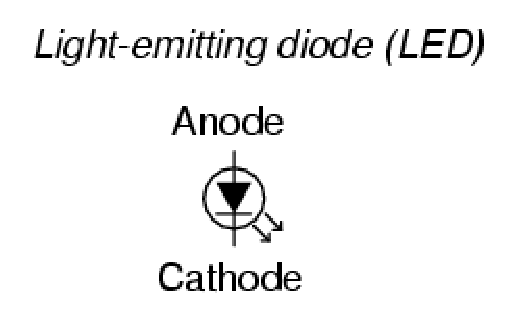
\includegraphics[scale=0.5]{../../epsimages/ledsym.eps}
\caption{Symbol for a light-emitting diode with anode and cathode labelled.}
\end{center}
\end{figure}

\Extension{Circuit Symbols}{This notation of having two small arrows pointing away from the device is common to the schematic symbols of all light-emitting semiconductor devices. Conversely, if a device is light-activated (meaning that incoming light stimulates it), then the symbol will have two small arrows pointing toward it. It is interesting to note, though, that LEDs are capable of acting as light-sensing devices: they will generate a small voltage when exposed to light, much like a solar cell on a small scale. This property can be gainfully applied in a variety of light-sensing circuits.}

The colour depends on the semiconducting material used to construct the LED, and can be in the near-ultraviolet, visible or infrared part of the electromagnetic spectrum.
 
\begin{IFact}{Nick Holonyak Jr. (1928) of the University of Illinois at Urbana-Champaign developed the first practical visible-spectrum LED in 1962.}
\end{IFact}

\subsubsection{Light emission}
The wavelength of the light emitted, and therefore its colour, depends on the materials forming the p-n junction. A normal diode, typically made of silicon or germanium, emits invisible far-infrared light (so it can't be seen), but the materials used for an LED can emit light corresponding to near-infrared, visible or near-ultraviolet frequencies.

\subsubsection{LED applications}
LEDs have many uses.  Some of these are given here.
\begin{itemize}
\item thin, lightweight message displays, e.g. in public information signs (at airports and railway stations, among other places)
\item status indicators, e.g. on/off lights on professional instruments and consumers audio/video equipment
\item infrared LEDs in remote controls (for TVs, VCRs, etc.)
\item clusters of LEDs are used in traffic signals, replacing ordinary bulbs behind coloured glass
\item car indicator lights and bicycle lighting
\item calculator and measurement instrument displays (seven segment displays), although now mostly replaced by LCDs
\item red or yellow LEDs are used in indicator and [alpha]numeric displays in environments where night vision must be retained: aircraft cockpits, submarine and ship bridges, astronomy observatories, and in the field, e.g. night time animal watching and military field use
\item red or yellow LEDs are also used in photographic darkrooms, for providing lighting which does not lead to unwanted exposure of the film
\item illumination, e.g. flashlights (a.k.a. torches, UK), and backlighting for LCD screens
\item signalling/emergency beacons and strobes
\item movement sensors, e.g. in mechanical and optical computer mice and trackballs
\item in LED printers, e.g. high-end colour printers
\end{itemize}

LEDs offer benefits in terms of maintenance and safety.

\begin{itemize}
\item The typical working lifetime of a device, including the bulb, is ten years, which is much longer than the lifetimes of most other light sources.
\item LEDs fail by dimming over time, rather than the abrupt burn-out of incandescent bulbs.
\item LEDs give off less heat than incandescent light bulbs and are less fragile than fluorescent lamps.
\item Since an individual device is smaller than a centimetre in length, LED-based light sources used for illumination and outdoor signals are built using clusters of tens of devices.
\end{itemize}

Because they are monochromatic, LED lights have great power advantages over white lights where a specific colour is required. Unlike the white lights, the LED does not need a filter that absorbs most of the emitted white light. Coloured fluorescent lights are made, but they are not widely available. LED lights are inherently coloured, and are available in a wide range of colours. One of the most recently introduced colours is the emerald green (bluish green, wavelength of about 500 nm) that meets the legal requirements for traffic signals and navigation lights. 

\begin{IFact}{The largest LED display in the world is 36~m high, at Times Square, New York, U.S.A.}
\end{IFact}

There are applications that specifically require light that does not contain any blue component. Examples are photographic darkroom safe lights, illumination in laboratories where certain photo-sensitive chemicals are used, and situations where dark adaptation (night vision) must be preserved, such as cockpit and bridge illumination, observatories, etc. Yellow LED lights are a good choice to meet these special requirements because the human eye is more sensitive to yellow light.

\Exercise{The Light Emitting Diode}{
\begin{enumerate}
\item{What is an LED?}
\item List 5 applications of LEDs.
\end{enumerate}

% Automatically inserted shortcodes - number to insert 2
\par \practiceinfo
\par \begin{tabular}[h]{cccccc}
% Question 1
(1.)	01jp	&
% Question 2
(2.)	01jq	&
\end{tabular}
% Automatically inserted shortcodes - number inserted 2
}

\subsection{Transistor}
The diode is the simplest semiconductor device, made up of a p-type semiconductor and an n-type semiconductor in contact. It can conduct in only one direction, but it cannot control the size of an electric current.  Transistors are more complicated electronic components which can control the size of the electric current flowing through them.  

This enables them to be used in amplifiers.  A small signal from a microphone or a radio antenna can be used to control the transistor.  In response, the transistor will then increase and decrease a much larger current which flows through the speakers.

\begin{IFact}{One of the earliest popular uses of transistors was in cheap and portable radios.  Before that, radios were much more expensive and contained glass valves which were fragile and needed replacing.  In some parts of the world you can still hear people talking about their `transistor' --- they mean their portable radio.}\end{IFact}

You can also use a small current to turn the transistor on and off.  The transistor then controls a more complicated or powerful current through other components.  When a transistor is used in this way it is said to be in {\bf switching} mode as it is acting as a remotely controlled switch.  As we shall see in the final sections of this chapter, switching circuits can be used in a computer to process and store digital information.  A computer would not work without the millions (or billions) of transistors in it.

There are two main types of transistor - bipolar transistors (NPN or PNP), and field effect transistors (FETs).  Both use doped semiconductors, but in different ways.  You are mainly required to know about field effect transistors (FETs), however we have to give a brief description of bipolar transistors so that you see the difference.

\subsubsection{Bipolar Transistors}

Bipolar transistors are made of a doped semiconductor `sandwich'.  In an NPN transistor, a very thin layer of p-type semiconductor is in between two thicker layers of n-type semiconductor.  This is shown in Figure~\ref{fig:NPNtrans}.  Similarly an PNP transistor consists of a very thin n-type layer in between two thicker layers of p-type semiconductor.

\begin{figure}[htbp]
\begin{center}
\begin{pspicture}(0,0)(7,3)

\psframe(2,1)(3,2.5)
\uput[r](2.3,1.6){N}
\psframe(3,1)(3.2,2.5)
\uput[r](2.8,1.6){P}
\psframe(3.2,1)(4.2,2.5)
\uput[r](3.5,1.6){N}

\psline(0,1.5)(2,1.5)
\uput[r](0,1.7){Emitter}
\psline(4.2,1.5)(6,1.5)
\uput[r](4.9,1.7){Collector}
\psline(3.1,1)(3.1,0.2)(4.5,0.2)
\uput[r](3.6,0.4){Base}

\end{pspicture}
\caption{An NPN transistor.  This is a type of bipolar transistor.}
\label{fig:NPNtrans}
\end{center}
\end{figure}

In an NPN transistor a small current of electrons flows from the emitter (E) to the base (B).  Simultaneously, a much larger current of electrons flows from the emitter (E) to the collector (C).  If you lower the number of electrons able to leave the transistor at the base (B), the transistor automatically reduces the number of electrons flowing from emitter (E) to collector (C).  Similarly, if you increase the current of electrons flowing out of the base (B), the transistor automatically also increases the current of electrons flowing from emitter (E) to collector (C).  The transistor is designed so that the current of electrons from emitter to collector ($I_{EC}$) is proportional to the current of electrons from emitter to base ($I_{EB}$).  The constant of proportionality is known as the {\bf current gain} $\beta$.  So $I_{EC} = \beta I_{EB}$.

How does it do it?  The answer comes from our work with diodes.  Electrons arriving at the emitter (n-type semiconductor) will naturally flow through into the central p-type since the base-emitter junction is forward biased.  However if none of these electrons are removed from the base, the electrons flowing into the base from the emitter will fill all of the available `holes'.  Accordingly, a large depletion band will be set up.  This will act as an insulator preventing current flow into the collector as well.  On the other hand, if the base is connected to a positive voltage, a small number of electrons will be removed by the base connection.  This will prevent the `holes' in the base becoming filled up, and no depletion band will form. While some electrons from the emitter leave via the base connection, the bulk of them flow straight on to the collector.  You may wonder how the electrons get from the base into the collector (it seems to be reverse biased).  The answer is complicated, but the important fact is that the p-type layer is extremely thin.  As long as there is no depletion layer, the bulk of the electrons will have no difficulty passing straight from the n-type emitter into the n-type collector.  A more satisfactory answer can be given to a university student once band theory has been explained.

Summing up, in an NPN transistor, a small flow of electrons from emitter (E) to base (B) allows a much larger flow of electrons from emitter (E) to collector (C).  Given that conventional current (flowing from $+$ to $-$) is in the opposite direction to electron flow, we say that a small conventional current from base to emitter allows a large current to flow from collector to emitter.

A PNP transistor works the other way.  A small conventional current from emitter to base allows a much larger conventional current to flow from emitter to collector.  The operation is more complicated to explain since the principal charge carrier in a PNP transistor is not the electron but the `hole'.

The operation of NPN and PNP transistors (in terms of conventional currents) is summarised in Figure~\ref{fig:transcur}.

\begin{figure}
\begin{center}
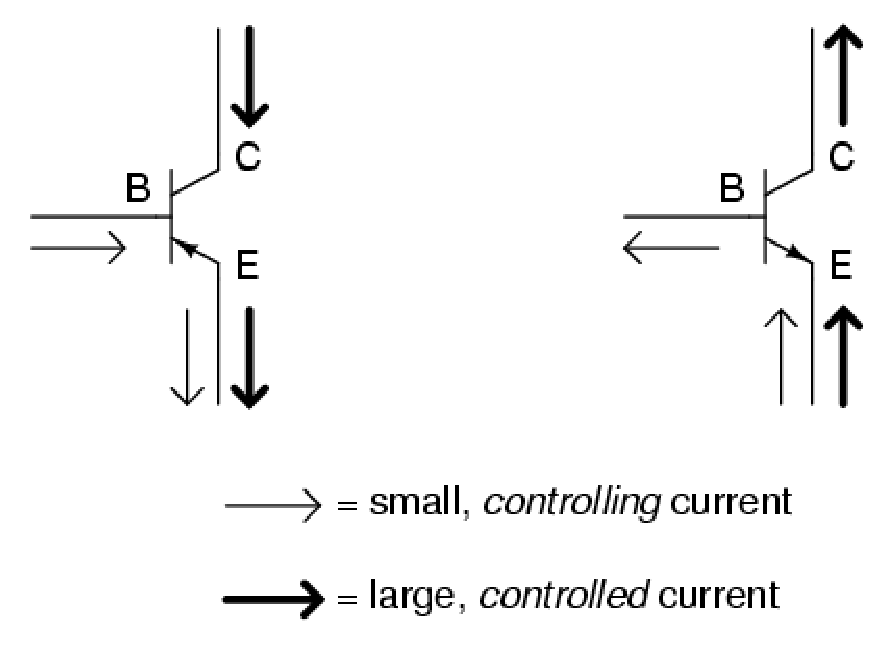
\includegraphics[scale=0.7]{../../epsimages/tranistorcurrents.eps}
\caption{An overview of bipolar transistors as current amplifiers. (Left) An NPN transistor. (Right) A PNP transistor.}
\label{fig:transcur}
\end{center}
\end{figure}

\begin{IFact}{The transistor is considered by many to be one of the greatest discoveries or inventions in modern history, ranking with banking and the printing press. Key to the importance of the transistor in modern society is its ability to be produced in huge numbers using simple techniques, resulting in vanishingly small prices. Computer ``chips'' consist of millions of transistors and sell for Rands, with per-transistor costs in the thousandths-of-cents. The low cost has meant that the transistor has become an almost universal tool for non-mechanical tasks. Whereas a common device, say a refrigerator, would have used a mechanical device for control, today it is often less expensive to simply use a few million transistors and the appropriate computer program to carry out the same task through "brute force". Today transistors have replaced almost all electromechanical devices, most simple feedback systems, and appear in huge numbers in everything from computers to cars.}\end{IFact} 


\subsubsection{The Field Effect Transistor (FET)}

To control a bipolar transistor, you control the {\bf current} flowing into or out of its base.  The other type of transistor is the field effect transistor (FET).  FETs work using control {\bf voltages} instead.  Accordingly they can be controlled with much smaller currents and are much more economic to use.  


\begin{figure}[htbp]
\begin{center} \begin{tabular}{cc}
\begin{pspicture}(0,1)(7,3.3)
\psframe(2,2)(5,3)
\uput[r](1.9,2.5){N}
\uput[r](4.4,2.5){N}
\psframe(2.5,2)(4.5,2.5)
\uput[r](3.3,2.3){P}
\uput[r](2.8,2.8){Channel}
\psline(0,2.5)(2,2.5)
\uput[r](0.0,2.7){Source}
\psline(5,2.5)(7,2.5)
\uput[r](6,2.7){Drain}
\psline(3.5,2)(3.5,1.2)(5.5,1.2)
\uput[r](5.2,1.4){Gate}
\end{pspicture} &
\begin{pspicture}(0,0.8)(5,4)
\pscircle(2,2){0.8}
\psline(0.5,1.5)(1.8,1.5)(1.8,2.5)
\psline(1.8,2.3)(2.2,2.3)(2.2,3.5)
\psline(1.8,1.7)(2.2,1.7)(2.2,0.9)
\uput[r](0.2,1.7){Gate}
\uput[r](2.1,1){Source}
\uput[r](2.1,3.6){Drain}
\end{pspicture} \\
\end{tabular}
\caption{A field effect transistor (FET).  The diagram on the left shows the semiconductor structure.  The diagram on the right shows its circuit symbol.}
\label{fig:fet}
\end{center}
\end{figure}

The three terminals of the FET are called the \textit{source} (S), \textit{drain} (D) and \textit{gate} (G), as shown in Figure~\ref{fig:fet}.  When the gate is not connected, a current of electrons can flow from source (S) to drain (D) easily along the channel.  The source is, accordingly, the negative terminal of the transistor.  The drain, where the electrons come out, is the positive terminal of the transistor.  A few electrons will flow from the n-type channel into the p-type semiconductor of the gate when the device is manufactured.  However, as these electrons are not removed (the gate is not connected), a depletion band is set up which prevents further flow into the gate.

\begin{IFact}{The transistor was invented at Bell Laboratories in December 1947 (first demonstrated on December 23) by John Bardeen, Walter Houser Brattain, and William Bradford Shockley, who were awarded the Nobel Prize in physics in 1956.}\end{IFact}
In operation, the gate is connected to negative voltages relative to the source.  This makes the p-n junction between gate and channel reverse-biased.  Accordingly no current flows from the source into the gate.  When the voltage of the gate is lowered (made more negative), the depletion band becomes wider.  This enlarged depletion band takes up some of the space of the channel.  So the lower the voltage of the gate (the more negative it is relative to the source), the larger the depletion band.  The larger the depletion band, the narrower the channel.  The narrower the channel, the harder it is for electrons to flow from source to drain.

\begin{IFact}{No-one would build a computer with billions of bipolar transistors --- the current in each transistor's base might be small, but when you add up all of the base currents in the millions of transistors, the computer as a whole would be consuming a great deal of electricity and making a great deal of heat.  Not only is this wasteful, it would prevent manufacturers making a computer of convenient size.  If the transistors were too close together, they would overheat.}\end{IFact}
The voltage of the gate is not the only factor affecting the current of electrons between the source and the drain.  If the external circuit has a low resistance, electrons are able to leave the drain easily.  If the external circuit has a high resistance, electrons leave the drain slowly.  This creates a kind of `traffic jam' which slows the passage of further electrons.  In this way, the voltage of the drain regulates itself, and is more or less independent of the current demanded from the drain.

Once these two factors have been taken into account, it is fair to say that the positive output voltage (the voltage of the drain relative to the source) is proportional to the negative input voltage (the voltage of the gate relative to the source).

For this reason, the field effect transistor is known as a voltage amplifier.  This contrasts with the bipolar transistor which is a current amplifier.

\Exercise{Field Effect Transistors}{
\begin{enumerate}
\item What are the two types of bipolar transistor?  How does their construction differ?
\item What are the three connections to a bipolar transistor called?
\item Why are very few electrons able to flow from emitter to collector in an NPN transistor if the base is not connected?
\item Why do you think a bipolar transistor would not work if the base layer were too thick?
\item ``The bipolar transistor is a current amplifier.''  What does this statement mean?
\item Describe the structure of a FET.
\item Define what is meant by the source, drain and gate.  During normal operation, what will the voltages of drain and gate be with respect to the source?
\item Describe how a depletion layer forms when the gate voltage is made more negative. What controls the width of the depletion layer?
\item ``The field effect transistor is a voltage amplifier.'' What does this statement mean?
\item The amplifier in a cheap radio will probably contain bipolar transistors.  A computer contains many field effect transistors.  Bipolar transistors are more rugged and less sensitive to interference than field effect transistors, which makes them more suitable for a simple radio.  Why are FETs preferred for the computer?
\end{enumerate}

% Automatically inserted shortcodes - number to insert 10
\par \practiceinfo
\par \begin{tabular}[h]{cccccc}
% Question 1
(1.)	01jr	&
% Question 2
(2.)	01js	&
% Question 3
(3.)	01jt	&
% Question 4
(4.)	01ju	&
% Question 5
(5.)	01jv	&
% Question 6
(6.)	01jw	\\ % End row of shortcodes
% Question 7
(7.)	01jx	&
% Question 8
(8.)	01jy	&
% Question 9
(9.)	01jz	&
% Question 10
(10.)	01k0	&
\end{tabular}
% Automatically inserted shortcodes - number inserted 10

}

\subsection{The Operational Amplifier}
%\begin{syllabus}
%\item The learner must be able to Explain that for mathematical operations such as multiplication and addition, a special amplifier is required.  Such a device is an operational amplifier or op-amp.
%\item Use the 741 op-amp as an example and explain that it has two input terminals called the inverting and non-inverting inputs.
%\item  Explain the need for a trimming potentiometer when using an op-amp.
%\end{syllabus}

The operational amplifier is a special kind of voltage amplifier which is made from a handful of bipolar or field effect transistors.  Operational amplifiers are usually called {\bf op-amps} for short.  They are used extensively in all kinds of audio equipment (amplifiers, mixers and so on) and in instrumentation.  They also have many other uses in other circuits - for example comparing voltages from sensors.

Operational amplifiers are supplied on Integrated Circuits (I.C.s).  The most famous operational amplifier I.C. is numbered 741 and contains a single operational amplifier on an integrated circuit (`chip') with eight terminals.  Other varieties can be bought, and you can get a single integrated circuit with two or four `741'-type operational amplifiers on it.

The symbol for an op-amp is shown in Figure~\ref{fig:opamp}. The operational amplifier has two input terminals and one output terminal.  The voltage of the output terminal is proportional to the difference in voltage between the two input terminals.  The output terminal is on the right (at the sharp point of the triangle).  The two input terminals are drawn on the left.  
One input terminal (labelled with a $+$ on diagrams) is called the {\bf non-inverting input}.  The other input terminal (labelled $-$) is called the {\bf inverting input}.  The labels $+$ and $-$ have nothing to do with the way in which the operational amplifier is connected to the power supply.  Operational amplifiers must be connected to the power supply, but this is taken for granted when circuit diagrams are drawn, and these connections are not shown on circuit diagrams.  Usually, when drawing electronic circuits, `0V' is taken to mean the negative terminal of the power supply.  This is not the case with op-amps.  For an op-amp, `0V' refers to the voltage midway between the $+$ and $-$ of the supply.

\begin{figure}[H]
\begin{center}
\begin{pspicture}(0,-0.6)(5,3.6)
%\psgrid[gridcolor=gray]
\pnode(0,0){A}
\pnode(0,3){B}
\pnode(5,1.5){C}
\OA(B)(A)(C)
\uput[dr](0,0){non-inverting input terminal}
\uput[ur](0,3){inverting input terminal}
\uput[r](5,1.5){output terminal}
\end{pspicture}
\caption{Circuit symbol for an operational amplifier.  The amplifier must also be connected to the $+$ and $-$ terminals of the power supply.  These connections are taken for granted and not shown.}
\label{fig:opamp}
\end{center}
\end{figure}

The output voltage of the amplifier $V_{out}$ is given by the formula
\equ{V_{out} = A \left( V_{+} - V_{-} \right)}
where $A$ is a constant called the {\bf open loop gain}, and $V_{+}$ and $V_{-}$ are the voltages of the two input terminals.  That said, the output voltage can not be less than the voltage of the negative terminal of the battery supplying it or higher than the positive terminal of the battery supplying it.  You will notice that $V_{out}$ is positive if $V_{+} > V_{-}$ and negative if $V_{+} < V_{-}$.  This is why the $-$ input is called the inverting input: raising its voltage causes the output voltage to {\it drop}.

The input resistance of an operational amplifier is very high.  This means that very little current flows into the input terminals during operation.

If all of the transistors in the operational amplifier were identical then the output voltage would be zero if the two inputs were at equal voltages.  In practise this is not quite the case, and for sensitive work a {\bf trimming potentiometer} is connected.  This is adjusted until the op-amp is zeroed correctly.  

Simple operational amplifiers require the trimming potentiometer to be built into the circuit containing them, and an example is shown in Figure~\ref{fig:invertamplifier}.  Other operational amplifier designs incorporate separate terminals for the trimming potentiometer.  These special terminals are labelled {\bf offset} on the manufacturer's diagram.  The exact method of connecting the potentiometer to the offset terminals can depend on the design of the operational amplifier, and you need to refer to the manufacturer's data sheet for details of which potentiometer to use and how to connect it.

For most commercially produced operational amplifiers (known as op-amps for short), the open loop gain $A$ is very large and does not stay constant.  Values of 100 000 are typical.  Usually a designer would want an amplifier with a stable gain of smaller value, and builds the operational amplifier into a circuit like the one in Figure~\ref{fig:invertamplifier}.


\begin{figure}[H]
\begin{center}
\begin{pspicture}(1,1)(10,7)
\psline(4,4)(4,6)(5.5,5)(4,4)
\uput[r](3.9,4.5){$+$}
\uput[r](3.9,5.5){$-$}
\psframe(2.5,5.3)(3.5,5.7)
\uput[r](2.6,5.9){$R_{1}$}
\psframe(4.2,6.5)(5.2,6.9)
\uput[r](4.3,7.1){$R_{2}$}
\psline(1.5,5.5)(2.5,5.5)
\uput[r](1.3,5.7){Input}
\psline(3.5,5.5)(4,5.5)
\psline(5.5,5)(7.5,5)
\uput[r](6.5,5.2){Output}
\psline(3.7,5.5)(3.7,6.7)(4.2,6.7)
\psline(5.2,6.7)(5.7,6.7)(5.7,5)

\psframe(2.8,1.5)(3.2,2.5)
\uput[r](2.1,2.0){$R_{3}$}
\psline{<-}(3.2,2)(3.7,2)
\psline(3.7,2)(3.7,4.5)(4,4.5)

\psline(1,2.2)(2,2.2)
\uput[r](1,2.4){$+$}
\psline(1.3,2)(1.7,2)
\psline(1.5,2.2)(1.5,3)(3,3)(3,2.5)
\psline(1.5,2)(1.5,1)(3,1)(3,1.5)
\end{pspicture}
\caption{An inverting amplifier built using an operational amplifier.  The connections from battery to operational amplifier are not shown.  The output voltage $V_{out} = - R_{2} V_{in} / R_{1}$, as explained in the text.  The potentiometer $R_{3}$ is a trimming potentiometer.  To set it, the input is connected to zero volts.  The trimming potentiometer is then adjusted until $V_{out} = 0$.  In all operational amplifier circuits, zero volts is midway between the $+$ and $-$ of the supply.}
\label{fig:invertamplifier}
\end{center}
\end{figure}



\Extension{Calculating the gain of the amplifier in Figure~\ref{fig:invertamplifier}.}{
\begin{enumerate}
\item The input resistance of the operational amplifier is very high.  This means that very little current flows into the inverting input of the op-amp.  Accordingly, the current through resistor $R_{1}$ must be almost the same as the current through resistor $R_{2}$.  This means that the ratio of the voltage across $R_{1}$ to the voltage across $R_{2}$ is the same as the ratio of the two resistances.
\item The open loop gain $A$ of the op-amp is very high.  Assuming that the output voltage is less than a few volts, this means that the two input terminals must be at very similar voltages.  We shall assume that they are at the same voltage.  
\item We want the output voltage to be zero if the input voltage is zero.  Assuming that the transistors within the op-amp are very similar, the output voltage will only be zero for zero input voltage if $V_{+}$ is very close to zero.  We shall assume that $V_{+}=0$ when the trimming potentiometer is correctly adjusted.
\item It follows from the last two statements that $V_{-} \approx 0$, and we shall assume that it is zero.
\item With these assumptions, the voltage across $R_{2}$ is the same as $V_{out}$, and the voltage across $R_{1}$ is the same as $V_{in}$.  Since both resistors carry the same current (as noted in point 1), we may say that the magnitude of $V_{out} / V_{in} = R_{2} / R_{1}$.  However, if $V_{in}$ is negative, then $V_{out}$ will be positive.  Therefore it is customary to write the gain of this circuit as $V_{out} / V_{in} = - R_{2} / R_{1}$.
\end{enumerate}}




\Exercise{Operational Amplifiers}{
\begin{enumerate}
\item What are operational amplifiers used for?
\item Draw a simple diagram of an operational amplifier and label its terminals.
\item  Why is a trimming potentiometer needed when using an op-amp?
\end{enumerate}

% Automatically inserted shortcodes - number to insert 3
\par \practiceinfo
\par \begin{tabular}[h]{cccccc}
% Question 1
(1.)	01k1	&
% Question 2
(2.)	01k2	&
% Question 3
(3.)	01k3	&
\end{tabular}
% Automatically inserted shortcodes - number inserted 3
}

\section{The Principles of Digital Electronics}
%\begin{syllabus}
%\item The learner must be able to Describe digital electronics as all-pervasive in modern technology: it is the ability to encode information with digital symbols that has made information processing the most important of modern technologies.
%\item The learner must be able to State that in digital electronics, two symbols are used: 1, which means "high" and 0, which means "low" (binary system).
%\item The learner must be able to Describe a logic gate as a device made with groups of transistors on a single chip called an integrated circuit (IC).
%\item The learner must be able to Recall the five main types of logic gates: i.e. NOT;  AND;  OR;  NAND;  NOR. Illustrate the correct symbol for each logic gate.
%\item The learner must be able to Compile the relevant truth table for each of the five logic gates.
%\item The learner must be able to Perform simple problem-solving exercises with two gates joined together to find the equivalent gate using truth tables.
%\item The learner must be able to Describe and explain how to use transistors to make a circuit that can count in the binary system.
%\end{syllabus}

The circuits and components we have discussed are very useful.  You can build a radio or television with them.  You can make a telephone.  Even if that was all there was to electronics, it would still be very useful.  However, the great breakthrough in the last fifty years or so has been in {\bf digital} electronics.  This is the subject which gave us the computer.  The computer has revolutionised the way business, engineering and science are done.  Small computers programmed to do a specific job (called microprocessors) are now used in almost every electronic machine from cars to washing machines.  Computers have also changed the way we communicate.  We used to have telegraph or telephone wires passing up and down a country --- each one carrying one telephone call or signal.  We now have optic fibres each capable of carrying tens of thousands of telephone calls using {\bf digital} signals.


So, what is a digital signal?  Look at Figure~\ref{fig:digitalanalogue}.  A normal signal, called an {\bf analogue} signal, carries a smooth wave.  At any time, the voltage of the signal could take any value.  It could be 2,00 V or 3,53 V or anything else.  A digital signal can only take certain voltages.  The simplest case is shown in the figure --- the voltage takes one of two values.  It is either {\bf high}, or it is {\bf low}.  It never has any other value.

These two special voltages are given symbols.  The low voltage level is written 0, while the high voltage level is written as 1.  When you send a digital signal, you set the voltage you want (0 or 1), then keep this fixed for a fixed amount of time (for example 0.01 $\mu$s), then you send the next 0 or 1.  The digital signal in Figure~\ref{fig:digitalanalogue} could be written 01100101.


\begin{figure}[H]
\begin{center}
\begin{pspicture}(0,-1)(12,6)
\psline[arrows=->](0,0)(5,0)
\uput[r](4,-0.2){time}
\psline[arrows=->](0,0)(0,4)
\uput[r](2,4.3){Analogue}

\pscurve(0,0)(1,3)(1.5,2)(2,2.5)(3,1.1)(3.5,0.3)(4,1.3)(4.5,2.4)(5,1.5)

\psline[arrows=->](7,0)(12,0)
\uput[r](11,-0.2){time}
\psline[arrows=->](7,0)(7,4)
\uput[r](9,4.3){Digital}

\uput[r](7.0,2){0}
\psline(7.5,0)(7.5,4)
\uput[r](7.5,2){1}
\uput[r](8.0,2){1}
\psline(7.5,4)(8.5,4)
\psline(8.5,0)(8.5,4)
\uput[r](8.5,2){0}
\uput[r](9.0,2){0}
\psline(9.5,0)(9.5,4)
\psline(9.5,4)(10.0,4)
\uput[r](9.5,2){1}
\psline(10.0,4)(10,0)
\uput[r](10.0,2){0}
\psline(10.5,0)(10.5,4)
\psline(10.5,4)(11,4)
\uput[r](10.5,2){1}
\end{pspicture}
\caption{The difference between normal (analogue) signals and digital signals. }
\label{fig:digitalanalogue}
\end{center}
\end{figure}

Why are digital signals so good?
\begin{enumerate}
\item Using a computer, any information can be turned into a pattern of 0s and 1s.  Pictures, recorded music, text and motion pictures can all be turned into a string of 0s and 1s and transmitted or stored in the same way.  The computer receiving the signal at the other end converts it back again.  A Compact Disc (CD) for example, can store music or text or pictures, and all can be read using a computer.
\item The 0 and the 1 look very different.  You can immediately tell if a 0 or a 1 is being sent.  Even if there is interference, you can still tell whether the sender sent a 0 or a 1.  This means that fewer mistakes are made when reading a digital signal.  This is why the best music recording technologies, and the most modern cameras, for example, all use digital technology.
\item Using the 0s and 1s you can count, and do all kinds of mathematics.  This will be explained in more detail in the next section.
\end{enumerate}

The simplest digital circuits are called {\bf logic gates}.  Each logic gate makes a decision based on the information it receives.  Different logic gates are set up to make the decisions in different ways.  Each logic gate will be made of many microscopic transistors connected together within a thin wafer of silicon.  This tiny circuit is called an Integrated Circuit or I.C. - all the parts are in one place (integrated) on the silicon wafer.  

\subsection{Logic Gates}
There are five main types of logic gate: NOT, AND, OR, NAND and NOR. Each one makes its decision in a different way.


\subsubsection{The NOT Gate}
{\bf Problem:} You want an automatic circuit in your office to turn on the heating in the winter.  You already have a digital electronic temperature sensor.  When the temperature is high, it sends out a 1.  When the office is cold, it sends out a 0.  If this signal were sent straight to the heater, the heater would turn on (1) when it was already hot, and would stay off when it was cold.  This is wrong!  To make the heater work, we need a circuit which will change a 0 (from the sensor) into a 1 (to send to the heater).  This will make the heater come on when it is cold. You also want it to change a 1 (from the sensor) into a 0 (to send to the heater).  This will turn the heater off when the room is hot.  This circuit is called an {\bf inverter} or {\bf NOT gate}.  It changes 0 into 1 (1 is NOT 0).  It changes 1 into 0 (0 is NOT 1).  It changes a signal into what it is NOT.

The symbol for the NOT gate is:

\begin{center}
\begin{pspicture}(0,0)(2.2,1.7)
\psline(0.5,0)(0.5,1)(1.5,0.5)(0.5,0)
\pscircle(1.6,0.5){0.1}
\psline(0,0.5)(0.5,0.5)
\psline(1.7,0.5)(2.5,0.5)
\end{pspicture}
\end{center}

The action of the NOT gate can be written in a table called a {\bf truth table}.  The left column shows the possible inputs on different rows.  The right column shows what the output (decision) of the circuit will be for that input.  The truth table for the NOT gate is shown below.

\begin{center}
\begin{tabular}{|c|c|}\hline
\textbf{Input} & \textbf{Output}\\\hline\hline
0&1\\\hline
1&0\\\hline
\end{tabular}
\end{center}

When you read the truth table, the top row says, ``If the input is 0, the output will be 1.''  For our heater, this means, ``If the room is cold, the heater will turn on.''  The bottom row says, ``If the input is 1, the output will be 0.''  For our heater, this means, ``If the room is hot, the heater will switch off.''

\subsubsection{The AND Gate}
{\bf Problem:} An airliner has two toilets.  Passengers get annoyed if they get up from their seat only to find that both toilets are being used and they have to go back to their seat and wait.  You want to fit an automatic circuit to light up a display if both toilets are in use.  Then passengers know that if the light is off, there will be a free toilet for them to use.  There is a sensor in each toilet.  It gives out a 0 of the toilet is free, and a 1 if it is in use.  You want to send a 1 to the display unit if {\bf both} sensors are sending 1s.  To do this, you use an AND gate.

The symbol for the AND gate is:

\begin{figure}[htbp]
\begin{center}
\begin{pspicture}(1.5,0)(4.5,2)
\psline(2.7,1.8)(2,1.8)(2,0.2)(2.7,0.2)
\psarc(2.7,1){0.8}{-90}{90}
\psline(1.5,0.5)(2,0.5)
\psline(1.5,1.5)(2,1.5)
\psline(3.5,1)(4.2,1)
\end{pspicture}
\caption{Symbol for the AND logic gate.}
\end{center}
\end{figure}

The truth table for the AND gate is shown below.  An AND gate has two inputs (the NOT gate only had one).  This means we need four rows in the truth table, one for each possible set of inputs.  The first row, for example, tells us what the AND gate will do if both inputs are 0.  In our airliner, this means that both toilets are free.  The right column has a 0 showing that the output will be 0, so the display will not light up.  The second row has inputs of 0 and 1 (the first toilet is free, the other is in use).  Again the output is 0.  The third row tells us what will happen if the inputs are 1 and 0 (the first toilet is in use, and the second is free).  Finally, the last line tells us what will happen if both inputs are 1 (the first toilet is in use and the second toilet is in use).  It is only in this case that the output is 1 and the display lights up.

\begin{center}
\begin{tabular}{|c|c|c|}\hline
\multicolumn{2}{|c|}{\textbf{Inputs}} & \textbf{Output}\\\hline
A&B& \\\hline\hline
0&0&0\\\hline
0&1&0\\\hline
1&0&0\\\hline
1&1&1\\\hline
\end{tabular}
\end{center}

This device is called an AND gate, because the output is only 1 if one input AND the other input are both 1.

\Extension{Using 0 and 1 to mean True and False}{When we use logic gates we use the low voltage state 0 to represent `false'.  The high voltage state 1 represents `true'.  This is why the word AND is so appropriate.  A AND B is true (1) if, and only if, A is true (1) AND B is true (1).}

\Extension{AND and multiplication}{Sometimes, the AND operation is written as multiplication.  A AND B is written AB.  If either A or B are 0, then AB will also be 0.  For AB to be 1, we need A and B to both be 1.  Multiplication of the numbers 0 and 1 does exactly the same job as an AND gate.}

\subsubsection{The NAND Gate}
{\bf Problem:} You build the circuit for the airliner toilets using an AND gate.  Your customer is pleased, but she says that it would be better if the display lit up when there {\bf was} a free toilet.  In other words, the display should light up unless both toilets are in use.  To do this we want a circuit which does the opposite of an AND gate.  We want a circuit which would give the output 0 where an AND gate would give 1.  We want a circuit which would give the output 1 where an AND gate would give 0.  This circuit is called a NAND gate.

The symbol for the NAND gate is:

\begin{figure}[H]
\begin{center}
\begin{pspicture}(1.5,0)(4.5,2)
\psline(2.7,1.8)(2,1.8)(2,0.2)(2.7,0.2)
\psarc(2.7,1){0.8}{-90}{90}
\pscircle(3.6,1){0.1}
\psline(1.5,0.5)(2,0.5)
\psline(1.5,1.5)(2,1.5)
\psline(3.7,1)(4.2,1)
\end{pspicture}
%\caption{Symbol for the NAND logic gate.}
\end{center}
\end{figure}

The truth table for the NAND gate is shown below.

\begin{center}
\begin{tabular}{|c|c|c|}\hline
\multicolumn{2}{|c|}{\textbf{Inputs}} & \textbf{Output}\\\hline
A&B& \\\hline\hline
0&0&1\\\hline
0&1&1\\\hline
1&0&1\\\hline
1&1&0\\\hline
\end{tabular}
\end{center}

You may have noticed that we could have done this job on the airliner by using our earlier circuit, with a NOT gate added between the original AND gate and the display.  This is where the word NAND comes from --- it is short for NotAND.

\subsubsection{The OR Gate}
{\bf Problem:} A long, dark corridor has two light switches --- one at each end of the corridor.  The switches each send an output of 0 to the control unit if no-one has pressed the switch.  If someone presses the switch, its output is 1.  The lights in the corridor should come on if either switch is pressed. To do this job, the control unit needs an OR gate. The symbol for the OR gate is:

\begin{figure}[H]
\begin{center}
\begin{pspicture}(1.5,0)(4.5,2)

\pscurve(2,0.2)(2.2,1)(2,1.8)
\pscurve(2,1.8)(3,1.5)(3.5,1)
\pscurve(2,0.2)(3,0.5)(3.5,1)

\psline(1.5,0.5)(2,0.5)
\psline(1.5,1.5)(2,1.5)
\psline(3.5,1)(4.2,1)
\end{pspicture}
\caption{Symbol for the OR logic gate.}
\end{center}
\end{figure}

The truth table for the OR gate is shown.

\begin{center}
\begin{tabular}{|c|c|c|}\hline
\multicolumn{2}{|c|}{\textbf{Inputs}} & \textbf{Output}\\\hline
A&B& \\\hline\hline
0&0&0\\\hline
0&1&1\\\hline
1&0&1\\\hline
1&1&1\\\hline
\end{tabular}
\end{center}

You can see that the output is 1 (and the lights come on in the corridor) if either one switch OR the other is pressed.  Pressing both switches also turns on the lights, as the last row in the table shows.

\Extension{OR and addition}{Sometimes you will see A OR B written mathematically as A+B.  This makes sense, since if A=0 and B=0, then A OR B = A+B = 0.  Similarly, if A=0 and B=1, then A OR B = A+B = 1.  If A=1 and B=0, then A OR B = A+B = 1 once again.  The only case where the OR function differs from normal addition is when A=1 and B=1.  Here A OR B = 1 in logic, but A+B=2 in arithmetic.  However, there is no such thing as `2' in logic, so we define + to mean `OR', and write 1+1=1 with impunity!


If you wish, you can prove that the normal rules of algebra still work using this notation:  A+(B+C) = (A+B)+C, A(BC) = (AB)C, and A(B+C) = AB + AC.  This special kind of algebra where variables can only be 0 (representing false) or 1 (representing true) is called Boolean algebra.}

\subsubsection{The NOR Gate}
The last gate you need to know is the NOR gate.  This is opposite to the OR gate.  The output is 1 if both inputs are 0.  In other words, the output switches on if neither the first NOR the second input is 1.  The symbol for the NOR gate is:

\begin{figure}{H}
\begin{center}
\begin{pspicture}(1.5,0)(4.5,2)

\pscurve(2,0.2)(2.2,1)(2,1.8)
\pscurve(2,1.8)(3,1.5)(3.5,1)
\pscurve(2,0.2)(3,0.5)(3.5,1)
\pscircle(3.6,1){0.1}
\psline(1.5,0.5)(2,0.5)
\psline(1.5,1.5)(2,1.5)
\psline(3.7,1)(4.2,1)
\end{pspicture}
\caption{Symbol for the NOR logic gate.}
\end{center}
\end{figure}

The truth table for the NOR gate is shown below.

\begin{center}
\begin{tabular}{|c|c|c|}\hline
\multicolumn{2}{|c|}{\textbf{Inputs}} & \textbf{Output}\\\hline
A&B& \\\hline\hline
0&0&1\\\hline
0&1&0\\\hline
1&0&0\\\hline
1&1&0\\\hline
\end{tabular}
\end{center}

The examples given were easy.  Each job only needed one logic gate.  However any `decision making' circuit can be built with logic gates, no matter how complicated the decision.  Here is an example.

\begin{wex}{An Economic Heating Control}{A sensor in a building detects whether a room is being used. If it is empty, the output is 0, if it is in use, the output is 1.  Another sensor measures the temperature of the room.  If it is cold, the output is 0.  If it is hot, the output is 1.  The heating comes on if it receives a 1.  Design a control circuit so that the heating only comes on if the room is in use and it is cold.}{The first sensor tells us whether the room is occupied.  The second sensor tells us whether the room is hot.  The heating must come on if the room is occupied AND cold.  This means that the heating should come on if the room is occupied AND (NOT hot).  To build the circuit, we first attach a NOT gate to the output of the temperature sensor.  This output of the NOT gate will be 1 only if the room is cold.  We then attach this output to an AND gate, together with the output from the other sensor. The output of the AND gate will only be 1 if the room is occupied AND the output of the NOT gate is also 1.  So the heating will only come on if the room is in use and is cold.  The circuit is shown below.

\begin{center}
\begin{pspicture}(0,0)(5.2,2)
\psline(2.7,1.8)(2,1.8)(2,0.2)(2.7,0.2)
\psarc(2.7,1){0.8}{-90}{90}
\psline(0,0.5)(2,0.5)
\uput[r](0,0.1){Occupied}
\psline(0,1.5)(0.9,1.5)
\uput[r](0,1.7){Hot}
\psline(0.9,1.8)(0.9,1.2)(1.5,1.5)(0.9,1.8)
\pscircle(1.6,1.5){0.1}
\psline(1.7,1.5)(2,1.5)
\psline(3.5,1)(4.2,1)
\uput[r](4.3,1){Output}
\end{pspicture}
\end{center}}
\end{wex}


\begin{wex}{Solving a circuit with two logic gates}{Compile the truth table for the circuit below.

\begin{center}
\begin{pspicture}(1.5,0)(6,2)
\pscurve(2,0.2)(2.2,1)(2,1.8)
\pscurve(2,1.8)(3,1.5)(3.5,1)
\pscurve(2,0.2)(3,0.5)(3.5,1)
\pscircle(3.6,1){0.1}
\psline(1.5,0.5)(2,0.5)
\psline(1.5,1.5)(2,1.5)
\psline(3.7,1)(4.2,1)
\psline(4.2,0.5)(4.2,1.5)(5.2,1)(4.2,0.5)
\pscircle(5.3,1){0.1}
\psline(5.4,1)(5.9,1)
\end{pspicture}
\end{center}
}{Firstly, we label the inputs A and B.  We also label the point where the two gates are connected C.
\begin{center}
\begin{pspicture}(1.2,0)(6.3,2)
\pscurve(2,0.2)(2.2,1)(2,1.8)
\pscurve(2,1.8)(3,1.5)(3.5,1)
\pscurve(2,0.2)(3,0.5)(3.5,1)
\pscircle(3.6,1){0.1}
\uput[r](0.9,0.5){A}
\psline(1.5,0.5)(2,0.5)
\uput[r](0.9,1.5){B}
\psline(1.5,1.5)(2,1.5)
\psline(3.7,1)(4.2,1)
\uput[r](3.6,1.2){C}
\psline(4.2,0.5)(4.2,1.5)(5.2,1)(4.2,0.5)
\pscircle(5.3,1){0.1}
\psline(5.4,1)(5.9,1)
\uput[r](5.5,1.2){Output}
\end{pspicture}
\end{center}
Next we prepare a truth table.  There is a column for each of the inputs, for the intermediate point C and also for the output.  The truth table has four rows, since there are four possible inputs --- 00, 01, 10 and 11.
\begin{center}
\begin{tabular}{|c|c|c|c|}\hline
A&B&C&Output\\\hline\hline
0&0& & \\\hline
0&1& & \\\hline
1&0& & \\\hline
1&1& & \\\hline
\end{tabular}
\end{center}
Next we fill in the C column given that we know what a NOR gate does.
\begin{center}
\begin{tabular}{|c|c|c|c|}\hline
A&B&C&Output\\\hline\hline
0&0&1& \\\hline
0&1&0& \\\hline
1&0&0& \\\hline
1&1&0& \\\hline
\end{tabular}
\end{center}
Next, we can fill in the output, since it will always be the opposite of C (because of the NOT gate).
\begin{center}
\begin{tabular}{|c|c|c|c|}\hline
A&B&C&Output\\\hline\hline
0&0&1&0\\\hline
0&1&0&1\\\hline
1&0&0&1\\\hline
1&1&0&1\\\hline
\end{tabular}
\end{center}
Finally we see that this combination of gates does the same job as an OR gate.
}
\end{wex}

Each logic gate is manufactured from two or more transistors.  Other circuits can be made using logic gates, as we shall see in the next section.  We shall show you how to count and store numbers using logic gates.  This means that if you have enough transistors, and you connect them correctly to make the right logic gates, you can make circuits which count and store numbers.

In practise, the cheapest gate to manufacture is usually the NAND gate. Additionally, Charles Peirce showed that NAND gates alone (as well as NOR gates alone) can be used to reproduce all the other logic gates.

\Exercise{The Principles of Digital Electronics}{
\begin{enumerate}
\item Why is digital electronics important to modern technology and information processing?
\item What two symbols are used in digital electronics, to represent a ``high" and a ``low"? What is this system known as?
\item What is a logic gate?
\item What are the five main types of logic gates? Draw the symbol for each logic gate.
\item Write out the truth tables for each of the five logic gates.
\item Write out the truth table for the following circuit.  Which single gate is this circuit equivalent to?
\begin{center}
\begin{pspicture}(1.5,0)(6.5,2)
\psline(2.7,1.8)(2,1.8)(2,0.2)(2.7,0.2)
\psarc(2.7,1){0.8}{-90}{90}
\pscircle(3.6,1){0.1}
\psline(1.5,0.5)(2,0.5)
\psline(1.5,1.5)(2,1.5)
\psline(3.7,1)(4.2,1)
\psline(4.2,1.5)(4.2,0.5)(5.2,1)(4.2,1.5)
\pscircle(5.3,1){0.1}
\psline(5.4,1)(6.4,1)
\end{pspicture}
\end{center}
\item Write out the truth table for the following circuit.  Which single gate is this circuit equivalent to?
\begin{center}
\begin{pspicture}(0,0)(4.5,2)

\pscurve(2,0.2)(2.2,1)(2,1.8)
\pscurve(2,1.8)(3,1.5)(3.5,1)
\pscurve(2,0.2)(3,0.5)(3.5,1)

\psline(1.5,0.5)(2,0.5)
\psline(1.5,1.5)(2,1.5)
\psline(3.5,1)(4.2,1)

\psline(1.3,0.5)(0.7,0.8)(0.7,0.2)(1.3,0.5)
\pscircle(1.4,0.5){0.1}
\psline(0,0.5)(0.7,0.5)

\psline(1.3,1.5)(0.7,1.8)(0.7,1.2)(1.3,1.5)
\pscircle(1.4,1.5){0.1}
\psline(0,1.5)(0.7,1.5)
\end{pspicture}
\end{center}
\end{enumerate}

% Automatically inserted shortcodes - number to insert 6
\par \practiceinfo
\par \begin{tabular}[h]{cccccc}
% Question 1
(1.)	01k4	&
% Question 2
(2.)	01k5	&
% Question 3
(3.)	01k6	&
% Question 4
(4.)	01k7	&
% Question 5
(5.)	01k8	&
% Question 6
(6.)	01k9	\\ % End row of shortcodes

(7.) aaa &
\end{tabular}
% Automatically inserted shortcodes - number inserted 6
}

\section{Using and Storing Binary Numbers}

%\begin{syllabus}
%\item The learner must be able to State that the basis of all computer memories is the bistable or flip-flop.
%\item The learner must be able to Demonstrate and explain that two NOR gates in series form a flip-flop and can remember one bit of information;
%\item The learner must be able to State that one bit is short for binary digit.
%\item The learner must be able to Demonstrate that all numbers can represented as binary numbers and be expressed in terms of 0s and 1s.
%\item The learner must be able to Show that counting circuits use flip-flops to "divide by two".
%\item The learner must be able to Describe that the modulo of a counter is the number of pulses needed to reset its output states to 0.  For example, a modulo counter counts up to seven then resets itself to zero.
%\item The learner must be able to Describe and explain a modulo 8 counter to allow counting from 0 (=000) to 7 (=111) using three flip-flops.
%\item The learner must be able to Explain that computers use millions of NOR gates to count.
%\item The learner must be able to Describe how to use NOR gates to make a circuit that can count
%\end{syllabus}

In the previous section, we saw how the numbers 0 and 1 could represent `false' and `true' and could be used in decision making.  Often we want to program a computer to count with numbers.  To do this we need a way of writing any number using nothing other than 0 and 1.  When written in this way, numbers are called {\bf binary numbers}.

\Definition{Binary Number System}{A way of writing any number using only the digits 0 and 1.}

\subsection{Binary numbers}

In normal (denary) numbers, we write 9+1 as 10.  The fact that the `1' in 10 is the second digit from the right tells us that it actually means 10 and not 1.  Similarly, the `3' in 365 represents 300 because it is the third digit from the right.  You could write 365 as $3 \times 100 + 6 \times 10 + 5$.  You will notice the pattern that the $n$th digit from the right represents $10^{n-1}$.  In binary, we use the $n$th digit from the right to represent $2^{n-1}$.  Thus 2 is written as 10 in binary.  Similarly $2^{2} = 4$ is written as 100 in binary, and $2^{3} = 8$ is written as 1000 in binary.

\begin{wex}{Conversion of Binary Numbers to Denary Numbers}{Convert the binary number 10101 to its denary equivalent.}{We start on the right.  The `1' on the right does indeed represent one.  The next `1' is in the third place from the right, and represents $2^2 = 4$.  The next `1' is in the fifth place from the right and represents $2^4 = 16$.  Accordingly, the binary number 10101 represents 16+4+1 = 21 in denary notation.}
\end{wex}


\begin{wex}{Conversion of Denary Numbers to Binary Numbers}{Convert the decimal number 12 to its binary equivalent.}{Firstly we write 12 as a sum of powers of 2, so 12 = 8+4.  In binary, eight is 1000, and four is 100.  This means that twelve = eight + four must be 1000+100 = 1100 in binary.  You could also write 12 as $1 \times 8 + 1 \times 4 + 0 \times 2 + 0 \times 1 = 1100$ in binary.}
\end{wex}

\begin{IFact}{How do you write numbers as a sum of powers of two?  The first power of two (the largest) is the largest power of two which is not larger than the number you are working with.  In our last example, where we wanted to know what twelve was in binary, the largest power of two which is not larger than 12 is 8.  Thus 12 = 8 + something.  By arithmetic, the `something' must be 4, and the largest power of two not larger than this is 4 exactly.  Thus 12 = 8 + 4, and we have finished.

A more complicated example would be to write one hundred in binary.  The largest power of two not larger than 100 is 64 (1000000 in binary).  Subtracting 64 from 100 leaves 36.  The largest power of two not larger than 36 is 32 (100000 in binary).  Removing this leaves a remainder of 4, which is a power of two itself (100 in binary).  Thus one hundred is 64 + 32 + 4, or in binary  1000000 + 100000 + 100 = 1100100.} \end{IFact}

Once a number is written in binary, it can be represented using the low and high voltage levels of digital electronics.  We demonstrate how this is done by showing you how an electronic counter works.

\subsection{Counting circuits}

To make a counter you need several `T flip flops', sometimes called `divide by two' circuits.  A T flip flop is a digital circuit which swaps its output (from 0 to 1 or from 1 to 0) whenever the input changes from 1 to 0.  When the input changes from 0 to 1 it doesn't change its output.  It is called a {\bf flip flop} because it changes (flips or flops) each time it receives a pulse.

If you put a series of pulses 10101010 into a T flip flop, the result is 01100110.  Figure~\ref{fig:Tinout} makes this clearer.

\begin{figure}[!h]
\begin{center}
\begin{pspicture}(-0.5,-1)(7,6)
\psline[arrows=->](0,0)(6,0)
\uput[r](6,0){time}
\uput[r](1,2.5){Output}

\psline(0.5,0)(0.5,2)
\psline(0.5,2)(1.5,2)
\psline(1.5,2)(1.5,0)
\psline(2.5,0)(2.5,2)
\psline(2.5,2)(3.5,2)
\psline(3.5,2)(3.5,0)

\psline[arrows=->](0,3)(6,3)
\uput[r](6,3){time}
\uput[r](1,5.5){Input}

\psline(0,3)(0,5)
\psline(0,5)(0.5,5)
\psline(0.5,5)(0.5,3)

\psline(1,3)(1,5)
\psline(1,5)(1.5,5)
\psline(1.5,5)(1.5,3)

\psline(2,3)(2,5)
\psline(2,5)(2.5,5)
\psline(2.5,5)(2.5,3)

\psline(3,3)(3,5)
\psline(3,5)(3.5,5)
\psline(3.5,5)(3.5,3)

\end{pspicture}
\caption{The output of a T flip flop, or `divide by two' circuit when a square wave is connected to the input.  The output changes state when the input goes from 1 to 0.}
\label{fig:Tinout}
\end{center}
\end{figure}

As you can see from Figure~\ref{fig:Tinout}, there are half as many pulses in the output.  This is why it is called a `divide by two' circuit.

If we connect T flip flops in a chain, then we make a counter which can count pulses.  As an example, we connect three T flip flops in a chain.  This is shown in Figure~\ref{fig:Tchain}.

\begin{figure}[!h]
\begin{center}
\begin{pspicture}(0,-1)(12,3.2)
\psframe(2,1)(4,3)
\uput[r](1.9,2){T}
\uput[r](3.4,2){Q}
\psline(0,2)(2,2)
\uput[r](0,2.4){Input}

\psframe(5,1)(7,3)
\uput[r](4.9,2){T}
\uput[r](6.4,2){Q}
\psline(4,2)(5,2)
\psline(4.5,2)(4.5,0)
\uput[r](4.2,-0.4){$Q_{0}$}

\psframe(8,1)(10,3)
\uput[r](7.9,2){T}
\uput[r](9.4,2){Q}
\psline(7,2)(8,2)
\psline(7.5,2)(7.5,0)
\uput[r](7.2,-0.4){$Q_{1}$}
\psline(10,2)(10.5,2)(10.5,0)
\uput[r](10.2,-0.4){$Q_{2}$}

\end{pspicture}
\caption{Three T flip flops connected together in a chain to make a counter.  The input of each flip flop is labelled T, while each output is labelled Q.  The pulses are connected to the input on the left.  The outputs $Q_{0}$, $Q_{1}$ and $Q_{2}$ give the three digits of the binary number as the pulses are counted.  This is explained in the text and in the next table.}
\label{fig:Tchain}
\end{center}
\end{figure}

When this circuit is fed with a stream of pulses, the outputs of the different stages change.  The table below shows how this happens.  Each row shows a different stage, with the first stage at the top.  We assume that all of the flip flops have 0 as their output to start with.

\begin{center} \begin{tabular}{|c|c|c|c|r|r|} \hline
Input & Output 1 & Output 2 & Output 3 & Number of pulse & Number in binary \\ \hline
1 & 0 & 0 & 0 & 0 & 000 \\ \hline
0 & 1 & 0 & 0 & 1 & 001 \\ \hline
1 & 1 & 0 & 0 & 1 & 001 \\ \hline
0 & 0 & 1 & 0 & 2 & 010 \\ \hline
1 & 0 & 1 & 0 & 2 & 010 \\ \hline
0 & 1 & 1 & 0 & 3 & 011 \\ \hline
1 & 1 & 1 & 0 & 3 & 011 \\ \hline
0 & 0 & 0 & 1 & 4 & 100 \\ \hline
1 & 0 & 0 & 1 & 4 & 100 \\ \hline
0 & 1 & 0 & 1 & 5 & 101 \\ \hline
1 & 1 & 0 & 1 & 5 & 101 \\ \hline
0 & 0 & 1 & 1 & 6 & 110 \\ \hline
1 & 0 & 1 & 1 & 6 & 110 \\ \hline
0 & 1 & 1 & 1 & 7 & 111 \\ \hline
1 & 1 & 1 & 1 & 7 & 111 \\ \hline
0 & 0 & 0 & 0 & 8 & 1000 \\ \hline
1 & 0 & 0 & 0 & 8 & 1000 \\ \hline
0 & 1 & 0 & 0 & 9 & 1101 \\ \hline
1 & 1 & 0 & 0 & 9 & 1101 \\ \hline \end{tabular} \end{center}
               
The binary numbers in the right hand column count the pulses arriving at the input.  You will notice that the output of the first flip flop gives the right most digit of the pulse count (in binary).  The output of the second flip flop gives the second digit from the right (the `twos' digit) of the pulse count.  The output of the third flip flop gives the third digit from the right (the `fours' digit) of the pulse count.  As there are only three flip flops, there is nothing to provide the next digit (the `eights' digit), and so the eighth pulse is recorded as 000, not 1000.

This device is called a {\bf modulo 8} counter because it can count in eight stages from 000 to 111 before it goes back to 000.  If you put four flip flops in the counter, it will count in sixteen stages from 0000 to 1111, and it is called a modulo 16 counter because it counts in sixteen stages before going back to 0000.

\Definition{Modulo}{The modulo of a counter tells you how many stages (or pulses) it receives before going back to 0 as its output.  Thus a modulo 8 counter counts in eight stages 000, 001, 010, 011, 100, 101, 110, 111, then returns to 000 again.}

\begin{IFact}{If a counter contains $n$ flip flops, it will be a modulo $2^{n}$ counter.  It will count from 0 to $2^{n} - 1$.}\end{IFact}

\subsection{Storing binary numbers}

Counting is important.  However, it is equally important to be able to remember the numbers.  Computers can convert almost anything to a string of 0s and 1s, and therefore to a binary number.  Unless this number can be stored in the computer's memory, the computer would be useless.

The memory in the computer contains many parts.  Each part is able to store a single 0 or 1.  Since 0 and 1 are the two binary digits, we say that each part of the memory stores one {\bf bit}.

\Definition{Bit}{One bit is a short way of saying one `binary digit'.  It is a single 0 or 1.}

\begin{IFact}{If you have eight bits, you can store a binary number from 00000000 to 11111111 (0 to 255 in denary).  This gives you enough permutations of 0s and 1s to have one for each letter of the alphabet (in upper and lower case), each digit from 0 to 9, each punctuation mark and each control code used by a computer in storing a document.  When you type text into a word processor, each character is stored as a set of eight bits.  Each set of eight bits is called a {\bf byte}.  Computer memories are graded according to how many bytes they store.  There are 1024 bytes in a kilobyte (kB), $1024 \times 1024$ bytes in a megabyte (MB), and $1024 \times 1024 \times 1024$ bytes in a gigabyte (GB).} \end{IFact}

To store a bit we need a circuit which can `remember' a 0 or a 1.  This is called a {\bf bistable} circuit because it has two stable states.  It can stay indefinitely either as a 0 or a 1.  An example of a bistable circuit is shown in Figure~\ref{fig:bistable}.  It is made from two NOR gates.

\begin{figure}[!h]
\begin{center}
\begin{tabular}{cc}
\begin{pspicture}(0,0)(6,6)

\pscurve(2,3.2)(2.2,4)(2,4.8)
\pscurve(2,4.8)(3,4.5)(3.5,4)
\pscurve(2,3.2)(3,3.5)(3.5,4)
\pscircle(3.6,4){0.1}

\psline(0.5,4.5)(2,4.5)
\uput[r](0,4.5){R}

\psline(3.7,4)(5,4)
\uput[r](5.2,4){Q}

\psline(4,4)(4,3)(1.5,2)(1.5,1.5)(2,1.5)
\psline[linewidth=0.1cm](3.7,1)(4,1)(4,2)(1.5,3)(1.5,3.5)(2,3.5)

\pscurve(2,0.2)(2.2,1)(2,1.8)
\pscurve(2,1.8)(3,1.5)(3.5,1)
\pscurve(2,0.2)(3,0.5)(3.5,1)
\pscircle(3.6,1){0.1}

\psline(0.5,0.5)(2,0.5)
\uput[r](0,0.5){S}
\end{pspicture} &

\begin{pspicture}(0,0)(6,6)

\pscurve(2,3.2)(2.2,4)(2,4.8)
\pscurve(2,4.8)(3,4.5)(3.5,4)
\pscurve(2,3.2)(3,3.5)(3.5,4)
\pscircle(3.6,4){0.1}

\psline(0.5,4.5)(2,4.5)
\uput[r](0,4.5){R}
\psline[linewidth=0.1cm](3.7,4)(5,4)
\uput[r](5.2,4){Q}

\psline[linewidth=0.1cm](4,4)(4,3)(1.5,2)(1.5,1.5)(2,1.5)
\psline(3.7,1)(4,1)(4,2)(1.5,3)(1.5,3.5)(2,3.5)

\pscurve(2,0.2)(2.2,1)(2,1.8)
\pscurve(2,1.8)(3,1.5)(3.5,1)
\pscurve(2,0.2)(3,0.5)(3.5,1)
\pscircle(3.6,1){0.1}

\psline(0.5,0.5)(2,0.5)
\uput[r](0,0.5){S}
\end{pspicture} \\ 
\end{tabular}
\caption{A bistable circuit made from two NOR gates.  This circuit is able to store one bit of digital information.  With the two inputs set to 0, you can see that the output could be (and will remain) either 0 or 1.  The circuit on the left shows an output of 0, the circuit on the right shows an output of 1.  Wires carrying high logic levels (1) are drawn thicker.  The output of the bistable is labelled Q.}
\label{fig:bistable}
\end{center}
\end{figure}

To store the 0 or the 1 in the bistable circuit, you set one of the inputs to 1, then put it back to 0 again.  If the input labelled `S' (set) is raised, the output will immediately become 1.  This is shown in Figure~\ref{fig:biS}.

\begin{figure}
\begin{center}
\begin{pspicture}(0,0)(6,6)
\pscurve(2,3.2)(2.2,4)(2,4.8)

\pscurve(2,4.8)(3,4.5)(3.5,4)
\pscurve(2,3.2)(3,3.5)(3.5,4)
\pscircle(3.6,4){0.1}

\psline(0.5,4.5)(2,4.5)
\uput[r](0,4.5){R}
\psline[linewidth=0.1cm](3.7,4)(5,4)
\uput[r](5.2,4){Q}

\psline[linewidth=0.1cm](4,4)(4,3)(1.5,2)(1.5,1.5)(2,1.5)
\psline(3.7,1)(4,1)(4,2)(1.5,3)(1.5,3.5)(2,3.5)

\pscurve(2,0.2)(2.2,1)(2,1.8)
\pscurve(2,1.8)(3,1.5)(3.5,1)
\pscurve(2,0.2)(3,0.5)(3.5,1)
\pscircle(3.6,1){0.1}

\psline[linewidth=0.1cm](0.5,0.5)(2,0.5)
\uput[r](0,0.5){S}
\end{pspicture}

\caption{The output of a bistable circuit is {\bf set} (made 1) by raising the `S' input to 1.  Wires carrying high logic levels (1) are shown with thicker lines.}
\label{fig:biS}
\end{center}
\end{figure}

To store a 0, you raise the `R' (reset) input to 1.  This is shown in Figure~\ref{fig:biR}.

\begin{figure}
\begin{center}
\begin{pspicture}(0,0)(6,6)

\pscurve(2,3.2)(2.2,4)(2,4.8)
\pscurve(2,4.8)(3,4.5)(3.5,4)
\pscurve(2,3.2)(3,3.5)(3.5,4)
\pscircle(3.6,4){0.1}

\psline[linewidth=0.1cm](0.5,4.5)(2,4.5)
\uput[r](0,4.5){R}

\psline(3.7,4)(5,4)
\uput[r](5.2,4){Q}

\psline(4,4)(4,3)(1.5,2)(1.5,1.5)(2,1.5)
\psline[linewidth=0.1cm](3.7,1)(4,1)(4,2)(1.5,3)(1.5,3.5)(2,3.5)

\pscurve(2,0.2)(2.2,1)(2,1.8)
\pscurve(2,1.8)(3,1.5)(3.5,1)
\pscurve(2,0.2)(3,0.5)(3.5,1)
\pscircle(3.6,1){0.1}

\psline(0.5,0.5)(2,0.5)
\uput[r](0,0.5){S}
\end{pspicture}

\caption{The output of a bistable circuit is {\bf reset} (made 0) by raising the `R' input to 1. Wires carrying high logic levels (1) are shown with thicker lines.}
\label{fig:biR}
\end{center}
\end{figure}

Once you have used the S or R inputs to set or reset the bistable circuit, you then bring both inputs back to 0.  The bistable `remembers' the state.  Because of the ease with which the circuit can be Reset and Set it is also called an {\bf RS flip flop} circuit.

Computer memory can store millions or billions of bits.  If it used our circuit above, it would need millions or billions of NOR gates, each of which is made from several transistors.  Computer memory is made of many millions of transistors.

\begin{IFact}{The bistable circuits drawn here don't remember 0s or 1s forever --- they lose the information if the power is turned off.  The same is true for the RAM (Random Access Memory) used to store working and temporary data in a computer.  Some modern circuits contain special memory which can remember its state even if the power is turned off.  This is used in FLASH drives, commonly found in USB data sticks and on the memory cards used with digital cameras.  These bistable circuits are much more complex.}  \end{IFact}

You can also make T flip flops out of logic gates, however these are more complicated to design.

\Exercise{Counting Circuits}{
\begin{enumerate}
\item What is the term \textit{bit} short for?
\item What is 43 in binary?
\item What is 1100101 in denary?
\item What is the highest number a modulo 64 counter can count to?  How many T flip flops does it contain?
\item What is the difference between an RS flip flop and a T flip flop?
\item Draw a circuit diagram for a bistable circuit (RS flip flop).  Make three extra copies of your diagram.  On the first diagram, colour in the wires which will carry high voltage levels (digital 1) if the R input is low, and the S input is high.  On the second diagram, colour in the wires which carry high voltage levels if the S input of the first circuit is now made low.  On the third diagram, colour in the wires which carry high voltage levels if the R input is now made high.  On the final diagram, colour in the wires carrying high voltage levels if the R input is now made low again.
\item Justify the statement: a modern computer contains millions of transistors.
\end{enumerate}

% Automatically inserted shortcodes - number to insert 7
\par \practiceinfo
\par \begin{tabular}[h]{cccccc}
% Question 1
(1.)	01ka	&
% Question 2
(2.)	01kb	&
% Question 3
(3.)	01kc	&
% Question 4
(4.)	01kd	&
% Question 5
(5.)	01ke	&
% Question 6
(6.)	01kf	\\ % End row of shortcodes
% Question 7
(7.)	01kg	&
\end{tabular}
% Automatically inserted shortcodes - number inserted 7
}


\Exercise{End of Chapter Exercises}{
\begin{enumerate}
\item Calculate the reactance of a 3 mH inductor at a frequency of 50 Hz.
\item Calculate the reactance of a 30 $\mu$F capacitor at a frequency of 1 kHz.
\item Calculate the impedance of a series circuit containing a 5 mH inductor, a 400 $\mu$F capacitor and a 2 k$\Omega$ resistor at a frequency of 50 kHz.
\item Calculate the frequency at which the impedance of the circuit in the previous question will be the smallest.
\item Which component can be used to block low frequencies?
\item Draw a circuit diagram with a battery, diode and resistor in series.  Make sure that the diode is forward biased so that a current will flow through it.
\item When building a complex electronic circuit which is going to be powered by a battery, it is always a good idea to put a diode in series with the battery.  Explain how this will protect the circuit if the user puts the battery in the wrong way round.
\item Summarise the differences between a bipolar and field effect transistor.
\item What does an operational amplifier (op-amp) do?
\item What is the difference between a digital signal and an analogue signal?
\item What are the advantages of digital signals over analogue signals?
\item Draw the symbols for the five logic gates, and write down their truth tables.
\item Draw a circuit diagram with an AND gate.  Each input should be connected to the output of a separate NOT gate.  By writing truth tables show that this whole circuit behaves as a NOR gate.
\item Convert the denary number 99 into binary.
\item Convert the binary number 11100111 into denary.
\item Explain how three T flip flops can be connected together to make a modulo 8 counter.  What is the highest number it can count up to?
\item Draw the circuit diagram for an RS flip flop (bistable) using two NOR gates.
\item Show how the circuit you have just drawn can have a stable output of 0 or 1 when both inputs are 0.
\item Operational (and other) amplifiers, logic gates, and flip flops all contain transistors, and would not work without them.  Write a short newspaper article for an intelligent reader who knows nothing about electronics. Explain how important transistors are in modern society.
\end{enumerate}

% Automatically inserted shortcodes - number to insert 19
\par \practiceinfo
\par \begin{tabular}[h]{cccccc}
% Question 1
(1.)	01kh	&
% Question 2
(2.)	01ki	&
% Question 3
(3.)	01kj	&
% Question 4
(4.)	01kk	&
% Question 5
(5.)	01km	&
% Question 6
(6.)	01kn	\\ % End row of shortcodes
% Question 7
(7.)	01kp	&
% Question 8
(8.)	01kq	&
% Question 9
(9.)	01kr	&
% Question 10
(10.)	01ks	&
% Question 11
(11.)	01kt	&
% Question 12
(12.)	01ku	\\ % End row of shortcodes
% Question 13
(13.)	01kv	&
% Question 14
(14.)	01kw	&
% Question 15
(15.)	01kx	&
% Question 16
(16.)	01ky	&
% Question 17
(17.)	01kz	&
% Question 18
(18.)	01m0	\\ % End row of shortcodes
% Question 19
(19.)	01m1	&
\end{tabular}
% Automatically inserted shortcodes - number inserted 19
}

% CHILD SECTION END 



% CHILD SECTION START 

\chapter[EM Radiation]{Electromagnetic Radiation}
\label{p:em:emr12}

\section{Introduction}
This chapter will focus on the electromagnetic (EM) radiation. Electromagnetic radiation is a self-propagating wave in space with electric and magnetic components. These components oscillate at right angles to each other and to the direction of propagation, and are in phase with each other. Electromagnetic radiation is classified into types according to the frequency of the wave: these types include, in order of increasing frequency, radio waves, microwaves, infrared radiation, visible light, ultraviolet radiation, X-rays and gamma rays.

\section{Particle/wave nature of electromagnetic radiation}
\label{p:em:emr12:d}
%\begin{syllabus}
%\item Explain that some aspects of the behaviour of EM radiation can best be explained using a wave model and some aspects can best be explained using a particle model
%\item Note: Link to Grade 12 Matter and Materials, photoelectric effect
%\end{syllabus}

If you watch a colony of ants walking up the wall, they look like a thin continuous black line.  But as you look closer, you see that the line is made up of thousands of separated black ants.

Light and all other types of electromagnetic radiation seems like a continuous wave at first, but when one performs experiments with light, one can notice that light can have both wave and particle like properties.  Just like the individual ants, the light can also be made up of individual bundles of energy, or quanta of light.

Light has both wave-like and particle-like properties (wave--particle duality), but only shows one or the other, depending on the kind of experiment we perform. A wave-type experiment shows the wave nature, and a particle-type experiment shows particle nature.  One cannot test the wave and the particle nature at the same time. A particle of light is called a photon.

\Definition{Photon}{A photon is a quantum (energy packet) of light.}

The particle nature of light can be demonstrated by the interaction of photons with matter.  One way in which light interacts with matter is via the photoelectric effect, which will be studied in detail in Chapter~\ref{p:mm:op12}.

\Exercise{Particle/wave nature of electromagnetic radiation}{
\begin{enumerate}
\item Give examples of the behaviour of EM radiation which can best be explained using a wave model.
\item Give examples of the behaviour of EM radiation which can best be explained using a particle model.
\end{enumerate}

% Automatically inserted shortcodes - number to insert 2
\par \practiceinfo
\par \begin{tabular}[h]{cccccc}
% Question 1
(1.)	01m2	&
% Question 2
(2.)	01m3	&
\end{tabular}
% Automatically inserted shortcodes - number inserted 2
}

\section{The wave nature of electromagnetic radiation}
%\begin{syllabus}
%\item as mutual induction of oscillating magnetic/electric fields
%\item Describe the source of electromagnetic waves as an accelerating charge
%\item Use words and diagrams to explain how an EM wave propagates when an electric field oscillating in one plane produces a magnetic field oscillating in a plane at right angles to it, which produces an oscillating electric field, and so on  
%\item State that these mutually regenerating fields travel through space at a constant speed of 3x108m/s, represented by c.
%\item Note: Mention that unlike sound waves, EM waves do not need a medium to travel through
%\end{syllabus}

Accelerating charges emit electromagnetic waves. We have seen that a changing electric field generates a magnetic field and a changing magnetic field generates an electric field. This is the principle behind the propagation of electromagnetic waves, because electromagnetic waves, unlike sound waves, do not need a medium to travel through. EM waves propagate when an electric field oscillating in one plane produces a magnetic field oscillating in a plane at right angles to it, which produces an oscillating electric field, and so on. The propagation of electromagnetic waves can be described as \textit{mutual induction}. 

These mutually regenerating fields travel through empty space at a constant speed of $3 \times 10^8\ems$, represented by $c$.

\begin{center}
\begin{pspicture}(-4,-4)(3,4)
\psset{Alpha=30}
\pstThreeDCoor[nameY=$B$,nameZ=$E$,linecolor=black,xMin=-4,yMin=-4,zMin=-4]
\parametricplotThreeD[xPlotpoints=200,linecolor=blue,linewidth=1.5pt,plotstyle=curve](-180,180){%
    t 60 div
    3 2.5 t mul cos mul
    0}
\parametricplotThreeD[xPlotpoints=200,linecolor=red,linewidth=1.5pt,plotstyle=curve](-180,180){%
    t 60 div
    0
     -3 2.5 t mul cos mul
    }
\end{pspicture}
\end{center}

%\begin{figure}[htp!]
%\nts{get this figure}%\includegraphics[width=0.75\textwidth]{../../epsimages/light-wave.eps}
%\label{ lightwave }
%\caption{ The propagation of electromagnetic waves }
%\end{figure}


\section{Electromagnetic spectrum}
\label{p:em:emr12:ems}

%\begin{syllabus}
%\item The learner given a list of different types of EM radiation, must be able to arrange them in order of frequency or wavelength.
%\item The learner Given the wavelength of EM waves, must be able to calculate the frequency and vice versa, using the equation c=f.lambda.
%\item The learner must be able to Give an example of the use of each type of EM radiation, i.e. gamma rays, X-rays, ultraviolet light, visible light, infrared, microwave and radio and TV waves.
%\item Note: Link to Grade 10 Waves, Sound and Light
%\end{syllabus}



\begin{figure}[htbp]
\begin{center}
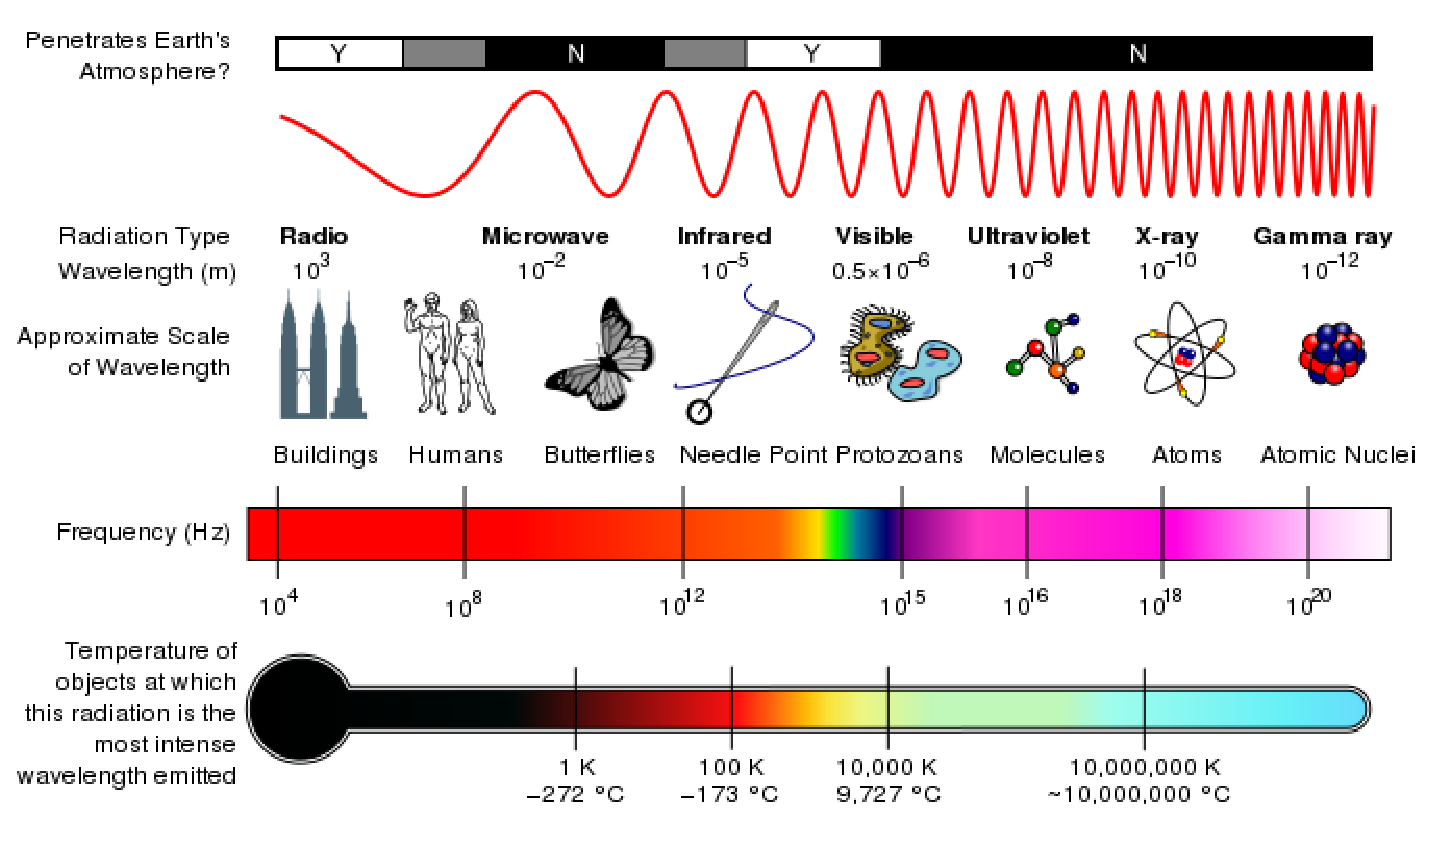
\includegraphics[width=0.95\textwidth]{../../epsimages/EM_Spectrum_Properties_edit.eps}%very big so leave out for now s}
\caption{The electromagnetic spectrum as a function of frequency. The different types according to wavelength are shown as well as everyday comparisons.}
\end{center}
\end{figure}

Observe the things around you, your friend sitting next to you, a large tree across the field. How is it that you are able to see these things? What is it that is leaving your friend's arm and entering your eye so that you can see his arm? It is light. The light originally comes from the sun, or possibly a light bulb or burning fire. In physics, light is given the more technical term electromagnetic radiation, which includes all forms of light, not just the form which you can see with your eyes. 

Electromagnetic radiation allows us to observe the world around us. It is this radiation which reflects off of the objects around you and into your eye. The radiation your eye is sensitive to is only a small fraction of the total radiation emitted in the physical universe. All of the different fractions taped together make up the electromagnetic spectrum. 

\Extension{Dispersion}{When white light is split into its component colours by a prism, you are looking at a portion of the electromagnetic spectrum.}

The wavelength of a particular electromagnetic radiation will depend on how it was created. 

\Exercise{Wave Nature of EM Radiation}{
\begin{enumerate}
\item List one source of electromagnetic waves. Hint: consider the spectrum diagram and look at the names we give to different wavelengths.
\item Explain how an EM wave propagates, with the aid of a diagram.
\item What is the speed of light? What symbol is used to refer to the speed of light? Does the speed of light change?
\item Do EM waves need a medium to travel through? 
\end{enumerate}

% Automatically inserted shortcodes - number to insert 4
\par \practiceinfo
\par \begin{tabular}[h]{cccccc}
% Question 1
(1.)	01m4	&
% Question 2
(2.)	01m5	&
% Question 3
(3.)	01m6	&
% Question 4
(4.)	01m7	&
\end{tabular}
% Automatically inserted shortcodes - number inserted 4

}

The radiation can take on any wavelength, which means that the spectrum is continuous. Physicists broke down this continuous band into sections. Each section is defined by how the radiation is created, not the wavelength of the radiation. But each category is continuous within the min and max wavelength of that category, meaning there are no wavelengths excluded within some range. 

The spectrum is in order of wavelength, with the shortest wavelength at one end and the longest wavelength at the other. The spectrum is then broken down into categories as detailed in Table~\ref{tab:emspectrum}.
\pagebreak
\begin{table}[htbp]
\begin{center}
\caption{Electromagnetic spectrum}
\label{tab:emspectrum}
\begin{tabular}{|c|c|c|}\hline
\textbf{Category}&\textbf{Range of Wavelengths (nm)}&\textbf{Range of Frequencies (Hz)}\\\hline\hline
gamma rays&$<$1&$>3\times 10^{19}$ \\\hline
X-rays&1-10&$3\times 10^{17}$-$3\times 10^{19}$\\\hline
ultraviolet light&10-400&$7,5\times 10^{14}$-$3\times 10^{17}$\\\hline
visible light&400-700&$4,3\times 10^{14}$-$7,5\times 10^{14}$\\\hline
infrared&700-$10^{5}$&$3\times 10^{12}$-$4,3\times 10^{19}$\\\hline
microwave&$10^{5}-10^{8}$&$3\times 10^{9}$-$3\times 10^{12}$\\\hline
radio waves&$>10^{8}$&$<3\times 10^{9}$\\\hline
\end{tabular}
\end{center}
\end{table}


Since an electromagnetic wave is still a wave, the following equation that you learnt in Grade 10 still applies:
\nequ{c=f\cdot \lambda}


\begin{wex}{EM spectrum I}{Calculate the frequency of red light with a wavelength of $4,2 \times 10^{-7}$~m}{ 
We use the formula: $c=f\lambda$ to calculate frequency. The speed of light is a constant $3 \times 10^{8}$m/s.
\begin{eqnarray*}
c&=&f\lambda\\
3 \times 10^{8}&=&f \times 4,2 \times 10^{-7} \\
f &=& 7,14 \times 10^{14} \rm {Hz}
\end{eqnarray*}}
\end{wex}

\begin{wex}{EM spectrum II}
{Ultraviolet radiation has a wavelength of $200~\mathrm{nm}$. What is the frequency of the radiation?}
{\westep{To calculate the frequency we need to identify the
wavelength and the velocity of the radiation.}
Recall that all radiation travels at the speed of light ($c$) in vacuum.
Since the question does not specify through what type of material the Ultraviolet radiation
is travelling, one can assume that it is travelling through a vacuum.
We can identify two properties of the radiation - $wavelength
~(200~\mathrm{nm})$ and speed ($c$).
%From previous chapters, we know that the period of the wave
%is the time it takes
%for a wave to complete one cycle or one wavelength. 

\westep{We can use the equation $c = f \lambda$ to find the frequency since the wavelength is given.}
\begin{eqnarray*}
c &=& f \lambda \\
3 \times 10^{8} &=& f \times 200 \times 10^{-9} \\
f &=&  1.5 \times 10^{15} \ \rm{Hz}
\end{eqnarray*}
}
\end{wex}



Examples of some uses of electromagnetic waves are shown in Table~\ref{tab:emuses}. 

\begin{table}[htbp]
\begin{center}
\caption{Uses of EM waves}
\label{tab:emuses}
\begin{tabular}{|c|p{5cm}|}\hline
\textbf{Category}&\textbf{Uses}\\\hline\hline
gamma rays&used to kill the bacteria in marshmallows and to sterilise medical equipment\\\hline
X-rays&used to image bone structures\\\hline
ultraviolet light&bees can see into the ultraviolet because flowers stand out more clearly at this frequency\\\hline
visible light&used by humans to observe the world\\\hline
infrared&night vision, heat sensors, laser metal cutting\\\hline
microwave&microwave ovens, radar\\\hline
radio waves&radio, television broadcasts\\\hline
\end{tabular}
\end{center}
\end{table}

In theory the spectrum is infinite, although realistically we can only observe wavelengths from a few hundred kilometers to those of gamma rays due to experimental limitations. 

Humans experience electromagnetic waves differently depending on their wavelength. Our eyes are sensitive to visible light while our skin is sensitive to infrared, and many wavelengths we do not detect at all.

\Exercise{EM Radiation}
{
\begin{enumerate}
\item Arrange the following types of EM radiation in order of increasing frequency: infrared, X-rays, ultraviolet, visible, gamma. 
\item Calculate the frequency of an EM wave with a wavelength of 400~nm.
\item Give an example of the use of each type of EM radiation, i.e. gamma rays, X-rays, ultraviolet light, visible light, infrared, microwave and radio and TV waves.
\end{enumerate}

% Automatically inserted shortcodes - number to insert 3
\par \practiceinfo
\par \begin{tabular}[h]{cccccc}
% Question 1
(1.)	01m8	&
% Question 2
(2.)	01m9	&
% Question 3
(3.)	01ma	&
\end{tabular}
% Automatically inserted shortcodes - number inserted 3
}

\section{The particle nature of electromagnetic radiation}
%\begin{syllabus}
%\item energy of a photon related to frequency and wavelength
%\item Calculate the energy of a photon using E = hf = hc/lambda
%\end{syllabus}

When we talk of electromagnetic radiation as a particle, we refer to photons, which are packets of energy. The energy of the photon is related to the wavelength of electromagnetic radiation according to:
%\equ{E=h\cdot f= \frac{hc}{\lambda}}{eq:ehf}
$h$ (called Planck's constant).






\Definition{Planck's constant}{Planck's constant is a physical constant named after Max Planck.

\nequ{h =6,626 \times 10^{-34}\ \mbox{J}\cdot\mbox{s}}
}

The energy of a photon can be calculated using the formula: $E=hf$ or $E=h \frac{c}{\lambda}$.
Where E is the energy of the photon in joules (J), h is planck's constant, c is the speed of light, f is the frequency in hertz (Hz) and $\lambda$ is the wavelength in metres (m).

\begin{wex}{Calculating the energy of a photon I}{Calculate the energy of a photon with a frequency of $3 \times 10^{18}$~Hz}
{
We use the formula: $E=hf$

\begin{eqnarray*}
E &=& hf\\
&=& 6,6 \times 10^{-34} \times 3 \times 10^{18}\\
&=& 2 \times 10^{-15} \eJ\\
\end{eqnarray*}}
\end{wex}

\begin{wex}{Calculating the energy of a photon II}
{What is the energy of an ultraviolet photon with a wavelength of 200~nm?}
{\westep{Determine what is required and how to approach the problem.}
We are required to calculate the energy associated with a photon of ultraviolet light with a wavelength of  200~nm.

We can use:
\nequ{E=h\frac{c}{\lambda}}

\westep{Solve the problem}
\begin{eqnarray*}
E & = & h\frac{c}{\lambda}\\
& = & (6,626 \times 10^{-34})\frac{3\times10^{8}}{200\times 10^{-9}}\\
& = & 9,939 \times 10^{-10}\eJ
\end{eqnarray*}}
\end{wex}


\Exercise{particle nature of EM waves}{
\begin{enumerate}
\item How is the energy of a photon related to its frequency and wavelength?
\item Calculate the energy of a photon of EM radiation with a frequency of $10^{12}$~Hz.
\item Determine the energy of a photon of EM radiation with a wavelength of 600 nm.
\end{enumerate}
\insertpracticeinfo{3}
}

\section{Penetrating ability of electromagnetic radiation}
\label{p:em:emr12:pa}
%\begin{syllabus}
%\item Indicate the penetrating ability of the different kinds of EM radiation and relate it to energy of the radiation.
%\item Describe the dangers of gamma rays, X-rays and the damaging effect of ultra-violet radiation on skin
%\item Note: Link to Grade 11 Matter and Materials, atomic nuclei
%\end{syllabus}

Different kinds of electromagnetic radiation have different penetrabilities. For example, if we take the human body as the object. Infrared light is emitted by the human body. Visible light is reflected off the surface of the human body, ultra-violet light (from sunlight) damages the skin, but X-rays are able to penetrate the skin and bone and allow for pictures of the inside of the human body to be taken.

If we compare the energy of visible light to the energy of X-rays, we find that X-rays have a much higher energy. Usually, kinds of electromagnetic radiation with higher energy have higher penetrabilities than those with low energies.

Certain kinds of electromagnetic radiation such as ultra-violet radiation, X-rays and gamma rays are very dangerous. Radiation such as these are called ionising radiation. Ionising radiation transfers energy as it passes through matter, breaking molecular bonds and creating ions.
 
Excessive exposure to radiation, including sunlight, X-rays and all nuclear radiation, can cause destruction of biological tissue. 

\subsection{Ultraviolet(UV) radiation and the skin}
UVA and UVB are different ranges of frequencies for ultraviolet (UV) light. UVA and UVB can damage collagen fibres which results in the speeding up skin aging. In general, UVA is the least harmful, but it  can contribute to the aging of skin, DNA damage and possibly skin cancer. It penetrates deeply and does not cause sunburn. Because it does not cause reddening of the skin (erythema) it cannot be measured in the SPF testing. There is no good clinical measurement of the blocking of UVA radiation, but it is important that sunscreen block both UVA and UVB.

UVB light can cause skin cancer. The radiation excites DNA molecules in skin cells, resulting in possible mutations, which can cause cancer. This cancer connection is one reason for concern about ozone depletion and the ozone hole.

As a defence against UV radiation, the body tans when exposed to moderate (depending on skin type) levels of radiation by releasing the brown pigment melanin. This helps to block UV penetration and prevent damage to the vulnerable skin tissues deeper down. Suntan lotion, often referred to as sunblock or sunscreen, partly blocks UV and is widely available. Most of these products contain an SPF rating that describes the amount of protection given. This protection, however, applies only to UVB rays responsible for sunburn and not to UVA rays that penetrate more deeply into the skin and may also be responsible for causing cancer and wrinkles. Some sunscreen lotion now includes compounds such as titanium dioxide which helps protect against UVA rays. Other UVA blocking compounds found in sunscreen include zinc oxide and avobenzone.

\Extension{What makes a good sunscreen?}{
\begin{itemize}
\item UVB protection: Padimate O, Homosalate, Octisalate (octyl salicylate), Octinoxate (octyl methoxycinnamate)
\item UVA protection: Avobenzone
\item UVA/UVB protection: Octocrylene, titanium dioxide, zinc oxide, Mexoryl (ecamsule)
\end{itemize}

Another means to block UV is by wearing sun protective clothing. This is clothing that has a UPF rating that describes the protection given against both UVA and UVB.}

\subsection{Ultraviolet radiation and the eyes}
High intensities of UVB light are hazardous to the eyes, and exposure can cause welder's flash (photo keratitis or arc eye) and may lead to cataracts, pterygium and pinguecula formation.

Protective eyewear is beneficial to those who are working with or those who might be exposed to ultraviolet radiation, particularly short wave UV. Given that light may reach the eye from the sides, full coverage eye protection is usually warranted if there is an increased risk of exposure, as in high altitude mountaineering. Mountaineers are exposed to higher than ordinary levels of UV radiation, both because there is less atmospheric filtering and because of reflection from snow and ice.

Ordinary, untreated eyeglasses give some protection. Most plastic lenses give more protection than glass lenses. Some plastic lens materials, such as polycarbonate, block most UV. There are protective treatments available for eyeglass lenses that need it which will give better protection. But even a treatment that completely blocks UV will not protect the eye from light that arrives around the lens. To convince yourself of the potential dangers of stray UV light, cover your lenses with something opaque, like aluminium foil, stand next to a bright light, and consider how much light you see, despite the complete blockage of the lenses. Most contact lenses help to protect the retina by absorbing UV radiation.

\subsection{X-rays}
While x-rays are used significantly in medicine, prolonged exposure to X-rays can lead to cell damage and cancer.

For example, a mammogram is an x-ray of the human breast to detect breast cancer, but if a woman starts having regular mammograms when she is too young, her chances of getting breast cancer increases.

\subsection{Gamma-rays}
Due to the high energy of gamma-rays, they are able to cause serious damage when absorbed by living cells.

Gamma-rays are not stopped by the skin and can induce DNA alteration by interfering with the genetic material of the cell. DNA double-strand breaks are generally accepted to be the most biologically significant lesion by which ionising radiation causes cancer and hereditary disease.

A study done on Russian nuclear workers exposed to external whole-body gamma-radiation at high cumulative doses shows a link between radiation exposure and death from leukaemia, lung, liver, skeletal and other solid cancers.


\Extension{Cellphones and electromagnetic radiation}{Cellphone radiation and health concerns have been raised, especially following the enormous increase in the use of wireless mobile telephony throughout the world. This is because mobile phones use electromagnetic waves in the microwave range. These concerns have induced a large body of research. Concerns about effects on health have also been raised regarding other digital wireless systems, such as data communication networks.
In 2009 the World Health Organisation announced that they have found a link between brain cancer and cellphones.

Cellphone users are recommended to minimise radiation, by for example:

\begin{enumerate}
\item Use hands-free to decrease the radiation to the head.
\item Keep the mobile phone away from the body.
\item Do not telephone in a car without an external antenna.
\end{enumerate}

}

\Exercise{}{
\begin{enumerate}
\item Indicate the penetrating ability of the different kinds of EM radiation and relate it to energy of the radiation.
\item Describe the dangers of gamma rays, X-rays and the damaging effect of ultra-violet radiation on skin
\end{enumerate}

% Automatically inserted shortcodes - number to insert 2
\par \practiceinfo
\par \begin{tabular}[h]{cccccc}
% Question 1
(1.)	01mb	&
% Question 2
(2.)	01mc	&
\end{tabular}
% Automatically inserted shortcodes - number inserted 2

}
% Presentation on the electromagnetic spectrum: SIYAVULA-PRESENTATION:http://cnx.org/content/m39513/latest/#slidesharefigure

\summary{VPpxh}
\begin{enumerate}
\item Electromagnetic radiation has both a wave and a particle nature.
\item Electromagnetic waves travel at a speed of $3 \times 10^{8}~m \cdot s^{-1}$ in a vacuum.
\item The Electromagnetic spectrum consists of the following types of radiation: radio waves, microwaves, infrared, visible, ultraviolet, X-rays, gamma-rays.
\item Gamma-rays have the most energy and are the most penetrating, while radio waves have the lowest energy and are the least penetrating.

\end{enumerate}

\begin{eocexercises}{}
\begin{enumerate}

\item What is the energy of a photon of EM radiation with a frequency of $3 \times 10^{8}$~Hz? 

\item What is the energy of a photon of light with a wavelength of 660~nm?

\item List the main types of electromagnetic radiation in order of increasing wavelength.

\item List the main uses of:
\begin{enumerate}
\item radio waves
\item infrared
\item gamma rays
\item X-rays
\end{enumerate}

\item Explain why we need to protect ourselves from ultraviolet radiation from the Sun.

\item List some advantages and disadvantages of using X-rays.

\item What precautions should we take when using cell phones?

\item Write a short essay on a type of electromagnetic waves. You should look at uses, advantages and disadvantages of your chosen radiation.

\item Explain why some types of electromagnetic radiation are more penetrating than others.

\end{enumerate}

% Automatically inserted shortcodes - number to insert 9
\par \practiceinfo
\par \begin{tabular}[h]{cccccc}
% Question 1
(1.)	01md	&
% Question 2
(2.)	01me	&
% Question 3
(3.)	01mf	&
% Question 4
(4.)	01mg	&
% Question 5
(5.)	01mh	&
% Question 6
(6.)	01mi	\\ % End row of shortcodes
% Question 7
(7.)	01mj	&
% Question 8
(8.)	01mk	&
% Question 9
(9.)	01mm	&
\end{tabular}
% Automatically inserted shortcodes - number inserted 9

\end{eocexercises}



% CHILD SECTION END 



% CHILD SECTION START 


  \chapter{Optical Phenomena and Properties of Matter}
\label{p:mm:op12}


%\begin{pspicture}
%\psspectrum[absorption,lines={400,434.8,476.2,526.3,588.2,666.7},lwidth=0.1](\linewidth,1)
%\end{pspicture}
%\psspectrum[element={Hg,Cd2+,W+}]
%\psspectrum[element=F](\linewidth,1)

\section {Introduction}
For centuries physicists argued about whether light was a particle or a wave. It was assumed that light could only be one or the other, but not both.
 
%In earlier chapters on waves (Chapters~\ref{p:wsl:tw10}, \ref{p:wsl:de12}, \ref{p:wsl:c12}, \ref{p:wsl:2d3d12}) and optics (Chapters~\ref{p:wsl:go10} and \ref{p:wsl:go11}), you studied how light or other electromagnetic radiation propagates like a wave. The wave nature of light was demonstrated by the propagation of light in examples such as diffraction, interference, and polarisation of light.

In earlier chapters on waves and optics, you studied how light or other electromagnetic radiation propagates like a wave. The wave nature of light was demonstrated by the propagation of light in examples such as diffraction, interference, and polarisation of light.

 
You also saw in Electromagnetic Radiation how light sometimes behaves as a particle. This chapter looks at evidence supporting the \textit{particle model of light}. The idea that light can have both wave and particle properties was one of the most important discoveries of the twentieth century.\\
\chapterstartvideo{VPpxi}
\section{The transmission and scattering of light}
%\begin{syllabus}
%\item Learners must be able to explain the interaction of uv and visible radiation with metals (reflection by absorbtion and and re-emission) in terms of the interaction with electromagnetic radiation
%\item Explain why the sky is blue
%\item Notes: Link the interaction of matter with light to the electronic properties of matter (grade 11 electrical conduction)
%\end{syllabus}

\subsection{Energy levels of an electron}
We have seen that the electrons in an atom have different energy levels. When the electron receives enough energy, it can jump up to a higher energy level. This is called \textit{'exciting'} the electron. When the electron in a high energy level sheds some energy, it drops to a lower energy level. 
 
We have also seen that the energy associated with light at a specific wavelength is given by:
\nequ{E=\frac{h c}{\lambda}.}\\
 
In the particle model of light, this means that each packet of light (photon) at a wavelength $\lambda$ has energy:
\nequ{E=\frac{h c}{\lambda}.}

For the electron to receive energy, it \textit{absorbs} a photon and gets its energy. When an electron loses energy to drop to a lower level, it \textit{emits} (gives off) a photon with that energy. 

\subsection{Interaction of light with metals}
When light encounters or passes through a material, the photons of the light interact with the atoms or molecules of the material.  Depending on the strength of the interactions and how often they happen, the light will pass through the material or be scattered in some other direction.
 
Each wavelength of light relates to a particular energy, and the closer that energy is to the energy difference between two of the levels of the atom, the likelier the photon is to interact with the atom.
 
When visible or ultraviolet (UV) radiation shines on a metal, the photons are \textit{absorbed} by the electrons in the metal. The electrons are then excited up to a higher energy level. When an electron returns to a lower energy level, another photon is emitted. This is how light appears to be \textbf{reflected} off a metal surface. 
 
In previous chapters, you have studied geometrical optics, which tells us what happens to rays of light when they are reflected off a surface or refracted through a lens.  That tells us what happens to light rays, made up of many photons, on a large scale.  If you look at a smaller level, i.e. on a microscopic scale, then reflection and refraction happen by all the photons interacting with the atoms of the lens or mirror.  The photons get absorbed and re-emitted many times before emerging as the finals rays of light that we see.
 
%The dependence of the scattering of light on the energy levels of the materials it encounters is responsible for many effects that we see in %everyday life.  
Scattering of light is responsible for many effects in everyday life.
We see that certain materials are red or blue, for example, since they contain materials that have energy level differences that correspond to the energies of the photons that make up red or blue light.  These materials then reflect the red or blue light and absorb the other wavelengths in the visible spectrum.  White objects reflect photons of all wavelengths in the visual spectrum, while black objects absorb these photons.

\begin{IFact}{Because a truly black object absorbs all the visual wavelengths of light, and does not re-emit photons at visual wavelengths, we can say that 'black' is not a colour itself, but rather a \textit{lack of} colour! Also, since black objects absorb visual light, they heat up more than objects of other colours which reflect light at certain wavelengths.}
\end{IFact}

\Activity{Investigation}{Reflection and absorption}
{
\Aim{Investigate the interaction of light with differently coloured metal objects}
\Apparatus{Find some differently coloured metal objects (at least 5) which will not be damaged if left in the sun for 15 minutes. Make sure to include at least one white item and one black item.}
\Method{At the start of your lesson set out your objects in direct sunlight. Leave them there for around 15 minutes.

Alternatively, if it is a sunny day, you can use your teachers' cars for this experiment - as long as there are some cars of different colours and they have been standing in direct sunlight for the same length of time! } 

After 15 minutes is up, touch each of the items/cars (be careful not to burn yourself!) and compare their temperatures (rate them from 1 to 5 with 1 being cold and 5 being very hot) in a table such as the example table below:

\begin{center}
\begin{tabular}{ | c | c | c |}
\hline
\textbf{Object} & \textbf{Colour} & \textbf{Temperature rating} \\ \hline \hline
e.g. car 1 & e.g. red & e.g. 3 \\ \hline
   &      &    \\
\hline
\end{tabular}
\end{center}

\textbf{Questions:}\\
\begin{enumerate}
\item Which object was the hottest and what was it made of?
\item Which object was the coolest and what was it made of?
\item How did the temperatures of the black and white objects compare to each other? (which one was hotter and which was cooler?)
\item Try to explain the reasons for the different temperatures of the objects with respect to their colours and the materials of which they are made. 
\end{enumerate}
}
 
Metals generally reflect most wavelengths of visible light, but they will reflect the light in a certain direction, given by the laws of reflection in geometrical optics.  This is different to most materials, like wood or fabric, which reflect light in all directions.  Metals have this property since they have electrons that are not bound to atoms and can move freely through the metal. This is unlike most other materials that have their electrons bound closely to the atoms.  These free electrons in metals can then absorb and reflect photons of a wide range of energies. 

\textit{Ultraviolet light} (which has shorter wavelengths than visible light) will pass through some substances, such as many plastics, because they do not have the right energy levels to absorb it and re-emit it. \textit{X-rays} (also short wavelengths) will also pass through most materials, since the energies of X-rays correspond to the energy levels of atomic nuclei.  Such nuclei are much smaller than atoms, so it is much less likely for an X-ray to hit a nucleus instead of the whole atom.

Most materials will absorb \textit{infrared radiation} (longer wavelengths than visible light), since the energies of that radiation often correspond to rotational or vibrational energy levels of molecules. 

\begin{figure}[!tb]
\begin{center}
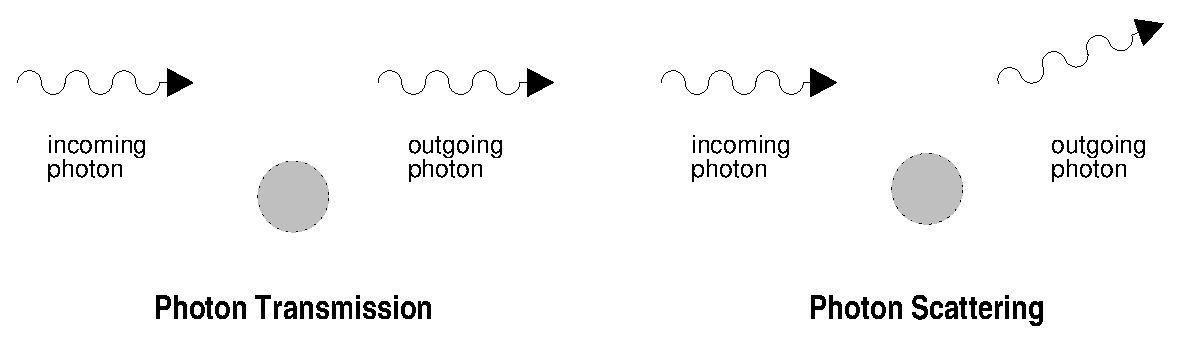
\includegraphics[width=4.5in]{../../epsimages/photon_scatter_transmission.eps}
\end{center}
\caption{Diagrams of photon transmission (left) and scattering (right).}
\label{transscatter}
\end{figure}

 
\subsection{Why is the sky blue?}
The sun emits light at many different wavelengths, including all of the visible wavelengths. Light which is made up of all the visible wavelengths appears white. So what causes the sky to look blue?

The atmosphere consists of molecules of different gases as well as tiny dust grains. Light from the sun scatters off the molecules in the air (called \textbf{Rayleigh scattering}).  
The chance that the light will scatter off the gas molecules is \textit{higher} for \textit{shorter} wavelengths.  The \textit{short wavelength} \textbf{blue light} is therefore scattered more than the other colours.  At noon, when the light from the sun is coming straight down (see the picture), the scattered blue light reaches your eyes from all directions and so the sky appears blue. The other wavelengths do not get scattered much and therefore miss your line of sight and are not seen. At sunrise or sunset, the direction of the light coming from the sun is now straight towards your eyes (see the picture). Therefore the scattered blue light can't be seen because it is scattered out of your line of sight. The redder colours (oranges and reds) can now be seen because they are not scattered as much and still fall in your line of sight. 
 


\begin{center}
\scalebox{1} % Change this value to rescale the drawing.
{
\begin{pspicture}(0,-2.38)(7.8,2.38)
\definecolor{color1652}{rgb}{0.6,0.6,0.6}
\psbezier[linewidth=0.04](1.34,-2.34)(1.76,-1.92)(5.06,-1.62)(6.04,-2.36)
\psbezier[linewidth=0.04](2.96,2.34)(3.04,1.66)(4.76,1.56)(4.88,2.36)
\psline[linewidth=0.04cm](2.98,2.04)(2.58,1.7)
\psline[linewidth=0.04cm](3.3,1.8)(3.02,1.4)
\psline[linewidth=0.04cm](3.66,1.74)(3.6,1.28)
\psline[linewidth=0.04cm](4.04,1.74)(4.1,1.24)
\psline[linewidth=0.04cm](4.42,1.8)(4.6,1.38)
\psline[linewidth=0.04cm](4.8,2.02)(5.18,1.6)
\psellipse[linewidth=0.04,dimen=outer](3.59,-1.14)(0.11,0.16)
\psline[linewidth=0.04cm](3.58,-1.28)(3.58,-1.68)
\psline[linewidth=0.04cm](3.58,-1.66)(3.72,-1.88)
\psline[linewidth=0.04cm](3.58,-1.68)(3.42,-1.88)
\psline[linewidth=0.04](3.44,-1.4)(3.58,-1.58)(3.72,-1.42)
\psbezier[linewidth=0.04,arrowsize=0.05291667cm 2.0,arrowlength=1.4,arrowinset=0.4]{->}(4.129678,1.802414)(4.0782003,1.7414411)(4.364416,1.3757231)(4.210351,1.3212587)(4.056286,1.2667943)(4.120731,0.99075055)(4.2747455,1.0081792)(4.42876,1.0256077)(4.4956264,0.6901674)(4.337112,0.66049534)(4.1785975,0.63082325)(4.251798,0.31939214)(4.4103127,0.34906423)(4.568827,0.3787363)(4.64,0.032700967)(4.4814854,0.003028889)(4.322971,-0.026643187)(4.496376,0.10848992)(4.567576,-0.46)
\psline[linewidth=0.05cm,linecolor=color1652,linestyle=dashed,dash=0.16cm 0.16cm](4.58,-0.46)(4.9,-1.86)
\psbezier[linewidth=0.04,arrowsize=0.05291667cm 3.0,arrowlength=1.4,arrowinset=0.4]{->}(4.54,-0.40787914)(4.4937525,-0.44371104)(4.4733295,-0.54631287)(4.441706,-0.4994201)(4.4100833,-0.45252737)(4.347896,-0.49794462)(4.3865466,-0.555258)(4.425197,-0.61257136)(4.366038,-0.6691876)(4.3282733,-0.61122465)(4.2905087,-0.55326164)(4.230578,-0.6134802)(4.2680573,-0.66905683)(4.3055367,-0.7246334)(4.2472634,-0.7806001)(4.2117267,-0.72315794)(4.1761894,-0.66571575)(4.1116886,-0.72194)(4.1515107,-0.7809901)(4.1913323,-0.84004027)(4.131117,-0.89787245)(4.0951796,-0.83509123)(4.0592427,-0.77230996)(4.000198,-0.83187896)(4.0369062,-0.89105785)(4.0736146,-0.95023674)(4.015341,-1.0062034)(3.9774616,-0.9452877)(3.939582,-0.88437206)(3.8797662,-0.9475433)(3.918417,-1.0048567)(3.9570677,-1.06217)(3.9199593,-0.99765205)(3.8193521,-1.1)
\psbezier[linewidth=0.04,arrowsize=0.05291667cm 2.0,arrowlength=1.4,arrowinset=0.4]{->}(4.563167,-0.42788064)(4.554229,-0.46518552)(4.770936,-0.6485422)(4.7138457,-0.68920416)(4.656756,-0.7298661)(4.7514534,-0.87855685)(4.817297,-0.85843486)(4.883141,-0.8383128)(4.993015,-1.0197747)(4.9280276,-1.0469913)(4.863041,-1.0742079)(4.970103,-1.2419266)(5.0350895,-1.21471)(5.100076,-1.1874933)(5.2144175,-1.3745377)(5.1494303,-1.4017544)(5.0844436,-1.428971)(5.131203,-1.342265)(5.2982745,-1.652659)
\rput(1.82,1.105){At noon, sun is overhead}
\rput(5.7,0.78){\footnotesize sun emits radiation}
\rput(5.69,0.48){\footnotesize of all wavelengths}
\rput(3.14,-0.3){\footnotesize blue light scattered}
\rput(2.85,-0.56){\footnotesize by large angle}
\rput(2.69,-0.86){\footnotesize into the eye}
\rput(6.34,-0.66){\footnotesize red light scattered little}
\rput(6.15,-0.94){\footnotesize and misses the eye}
\end{pspicture} 
}
\end{center}

\begin{center}
\scalebox{1} % Change this value to rescale the drawing.
{
\begin{pspicture}(0,-1.96)(8.5465355,1.98)
\definecolor{color1960}{rgb}{0.6,0.6,0.6}
\psbezier[linewidth=0.04](1.24,-1.7)(1.66,-1.28)(4.96,-0.98)(5.94,-1.72)
\psbezier[linewidth=0.04](8.513465,0.21002984)(7.8331804,0.1324845)(7.7269735,-1.5871434)(8.526535,-1.7100298)
\psline[linewidth=0.04cm](8.22,0.12)(7.8,0.62)
\psline[linewidth=0.04cm](8.010457,-0.21053997)(7.4895434,0.09053997)
\psline[linewidth=0.04cm](7.92,-0.5)(7.32,-0.4)
\psline[linewidth=0.04cm](7.9,-0.86)(7.32,-0.96)
\psline[linewidth=0.04cm](8.02,-1.3)(7.52,-1.52)
\psline[linewidth=0.04cm](8.18,-1.62)(7.82,-1.94)
\psellipse[linewidth=0.04,dimen=outer](3.81,-0.52)(0.11,0.16)
\psline[linewidth=0.04cm](3.8,-0.66)(3.8,-1.06)
\psline[linewidth=0.04cm](3.8,-1.04)(3.94,-1.26)
\psline[linewidth=0.04cm](3.8,-1.06)(3.64,-1.26)
\psline[linewidth=0.04](3.66,-0.78)(3.8,-0.96)(3.94,-0.8)
\psbezier[linewidth=0.04,arrowsize=0.05291667cm 2.0,arrowlength=1.4,arrowinset=0.4]{->}(7.9119506,-0.8102876)(7.8759775,-0.73905927)(7.4274335,-0.85938114)(7.4375854,-0.696288)(7.447737,-0.5331948)(7.1684833,-0.48450622)(7.124267,-0.6330632)(7.0800514,-0.7816202)(6.745188,-0.7119222)(6.7798967,-0.5544338)(6.8146057,-0.39694548)(6.4993596,-0.34247005)(6.4646506,-0.49995843)(6.4299417,-0.6574468)(6.083643,-0.5875668)(6.118352,-0.43007845)(6.153061,-0.27259007)(6.2095814,-0.48504156)(5.658549,-0.32815576)
\psline[linewidth=0.05cm,linecolor=color1960,linestyle=dashed,dash=0.16cm 0.16cm](5.653688,-0.33958933)(4.2400846,-0.08635944)
\psbezier[linewidth=0.04,arrowsize=0.05291667cm 3.0,arrowlength=1.4,arrowinset=0.4]{->}(5.7173038,-0.32316893)(5.702421,-0.26658913)(5.615988,-0.20765318)(5.6715145,-0.19689642)(5.7270417,-0.18613966)(5.709574,-0.11114067)(5.641708,-0.12428783)(5.5738416,-0.13743499)(5.544883,-0.060840968)(5.6130004,-0.048763357)(5.681118,-0.036685742)(5.649146,0.042027358)(5.5833364,0.0292786)(5.5175266,0.016529841)(5.488819,0.092054315)(5.555586,0.102285594)(5.6223526,0.112516865)(5.5958447,0.1938731)(5.525922,0.18032755)(5.4559984,0.16678199)(5.4263344,0.24482395)(5.4981713,0.25333455)(5.570008,0.26184514)(5.538287,0.3394887)(5.469464,0.328859)(5.4006405,0.31822935)(5.3719335,0.3937538)(5.442813,0.40478188)(5.513693,0.41580996)(5.4789586,0.4955726)(5.4110923,0.48242545)(5.343226,0.46927828)(5.4171195,0.47818726)(5.36229,0.610817)
\psbezier[linewidth=0.04,arrowsize=0.05291667cm 2.0,arrowlength=1.4,arrowinset=0.4]{->}(5.6898327,-0.33666438)(5.658998,-0.31384376)(5.405474,-0.44154257)(5.3903885,-0.37309492)(5.375303,-0.30464724)(5.2014155,-0.33362415)(5.1941733,-0.4020921)(5.1869316,-0.47056004)(4.9769473,-0.50068235)(4.977325,-0.43022746)(4.9777026,-0.35977256)(4.7814665,-0.3926839)(4.781089,-0.4631388)(4.780711,-0.5335937)(4.563842,-0.5656432)(4.5642195,-0.49518833)(4.564597,-0.42473343)(4.6260986,-0.50168794)(4.2750816,-0.53400683)
\rput(2.54,1.785){At sunrise/sunset, sun is at horizon}
\rput(6.3,1.36){\footnotesize blue light scattered}
\rput(6.03,1.06){\footnotesize by large angle}
\rput(6.31,0.74){\footnotesize away from the eye}
\rput(5.25,-0.76){\footnotesize red light scattered}
\rput(4.89,-1.04){\footnotesize into the eye}
\end{pspicture} 
}
\end{center}

\Exercise{Transmission and scattering of light}{
\begin{enumerate}
\item{Explain how visible light is reflected from metals.}
\item{Explain why the sky is blue.}
\end{enumerate}

% Automatically inserted shortcodes - number to insert 2
\par \practiceinfo
\par \begin{tabular}[h]{cccccc}
% Question 1
(1.)	01mn	&
% Question 2
(2.)	01mp	&
\end{tabular}
% Automatically inserted shortcodes - number inserted 2
}

\section{The photoelectric effect}

Around the turn of the twentieth century, it was observed by a number of physicists (including Hertz, Thomson and Von Lenard) that when light was shone on a metal, electrons were emitted by the metal. This is called the photoelectric effect. (\textit{photo}- for light, \textit{electric}- for the electron.)

\Definition{The photoelectric effect}{The photoelectric effect is the process whereby an electron is emitted by a metal when light shines on it.}


At that time, light was thought to be purely a wave. Therefore, physicists thought that if a more intense (i.e. brighter) light was shone on a metal, then the electrons would be knocked out with greater kinetic energies than if a faint light was shone on them. However, Von Lenard observed that this did not happen at all. The \textit{intensity} of the light made \textit{no difference} to the kinetic energy of the emitted electrons! Also, it was observed that the electrons were emitted immediately when light was shone on the metal - there was no time delay.

Einstein solved this problem by proposing that light is made up of packets of energy called \textit{quanta} (now called photons) which interacted with the electrons in the metal like particles instead of waves. Each incident photon would transfer all its energy to one electron in the metal. For a specific colour of light (i.e. a certain wavelength or frequency), the energy of the photons is given by $E = hf = hc/\lambda$, where $h$ is Planck's constant. The energy needed to knock an electron out of the metal is called the \textbf{work function} (symbol $\phi$) of the metal. Therefore, the amount of energy left over as the kinetic energy ($E_{k}$) of the emitted electron would be the difference between the incoming photon's energy and the energy needed to knock out the electron (work function of the metal): 

\begin{eqnarray*}
E_{k} &=& hf - \phi 
\end{eqnarray*} 

Increasing the intensity of the light (i.e. making it brighter) did not change the wavelength of the light and therefore the electrons would be emitted with \textit{the same} kinetic energy as before! This solved the paradox and showed that light has \textit{both} a \textbf{wave nature} and a \textbf{particle nature}. Einstein won the Nobel prize for this quantum theory and his explanation of the photoelectric effect. 

Increasing the intensity of the light actually means increasing the \textit{number} of incident photons. Therefore, since each photon only gives energy to one electron, more incident photons means \textit{more} electrons would be knocked out of the metal, but their kinetic energies would be \textit{the same} as before. 

\begin{figure}[!h]
\begin{center}
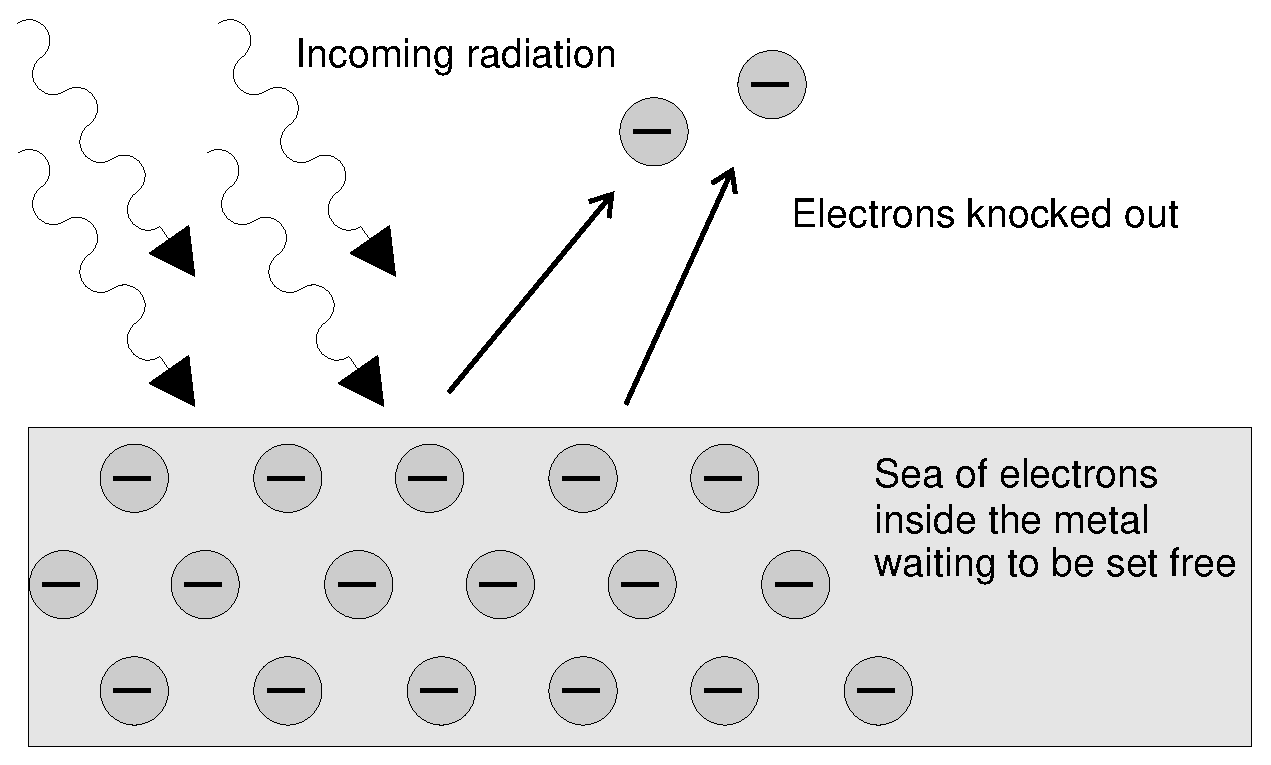
\includegraphics[width=0.5\textwidth]{../../epsimages/Photoelectric_effect.eps}
\caption{The photoelectric effect: Incoming photons on the left hit the electrons inside the metal surface. The electrons absorb the energy from the photons, and are ejected from the metal surface.}
\label{phot_el}
\end{center}
\end{figure}

\begin{IFact}
{The photoelectric effect was first observed in the experiments of Heinrich Hertz in 1887. In 1899 J.J. Thomson proved that it was electrons that were emitted. The photoelectric effect was theoretically explained by Albert Einstein in 1905.}
\end{IFact}
% Phet simulation on the photoelectric effect: SIYAVULA-SIMULATION:http://cnx.org/content/m39551/latest/#id63458

\simulation{phet on photoelectric}{VPpyy}
 
The discovery and understanding of the photoelectric effect was one of the major breakthroughs in science in the twentieth century as it provided concrete evidence of the particle nature of light. It overturned previously held views that light was composed purely of a continuous transverse wave. On the one hand, the wave nature is a good description of phenomena such as diffraction and interference for light, and on the other hand, the photoelectric effect demonstrates the particle nature of light. This is now known as the `dual-nature' of light. (dual means two)

%The new picture considered light (or in general, electromagnetic radiation) to be composed of several 'packets' or 'quanta' (plural for %'quantum') of energy. Each individual photon had a fixed amount of energy depending on the frequency of the electromagnetic radiation.
%However, the wave nature of electromagnetic radiation was also valid since phenomena such as diffraction and interference could only be %explained using the wave nature as they are basic wave properties. Hence a general agreement was reached that light (all electromagnetic %radiations) exhibits a dual nature. Light behave as waves in some cases and behaves as particles in other cases. This came to be known as the %'dual-nature of light'. This  dual-nature of light and all other electromagnetic radiations forms the backbone of quantum mechanics . Note that %the energy of quanta is quantised ($E = hf$) which means that the energy can have a value only in multiples of $h$ (Planck's constant). 
 
While solving problems we need to decide for ourselves whether we should consider the wave property or the particle property of light. For example, when dealing with interference and diffraction, light should be treated as a wave, whereas when dealing with photoelectric effect we consider the particle nature.
 
\subsection{Applications of the photoelectric effect}

%\begin{figure}[htbp]
%\begin{center}
%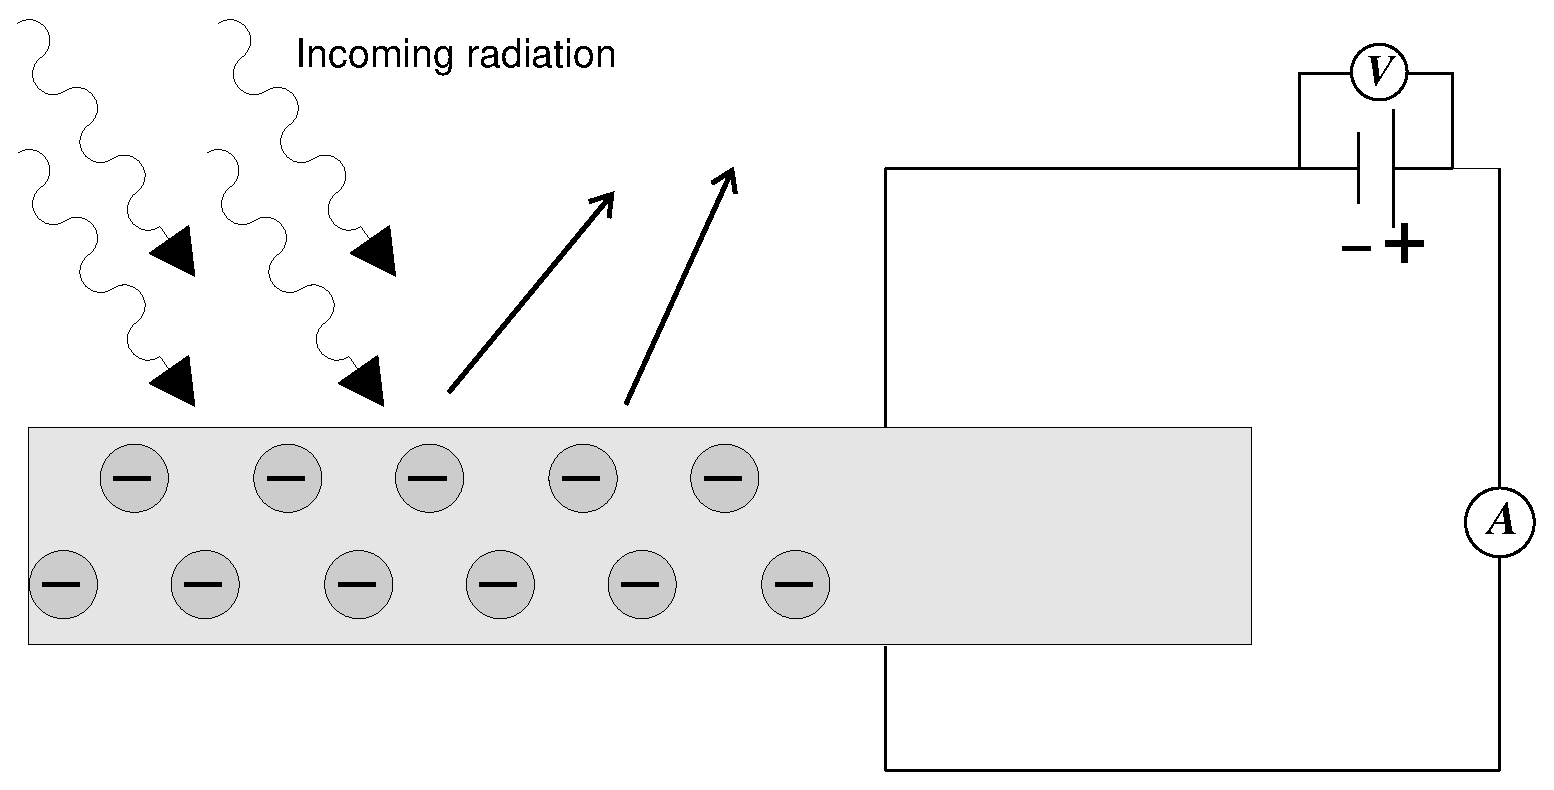
\includegraphics[width=0.4\textwidth]{../../epsimages/electFromSurface.eps}
%\caption{Diagram of a circuit to measure the photoelectric effect. If the photons on the left eject electrons from the metal foil, the metal %foil will lose some negative charge carriers. New negative charges will flow toward the metal foil to replace the lost electrons, and a current %will be measured by the ammeter in the circuit.}
%\label{elec_cir}
%\end{center}
%\end{figure}

We have learnt that a metal contains electrons that are free to move between the valence and conduction bands. When a photon strikes the surface of a metal, it gives \textit{all} its energy to one electron in the metal. 
\begin{itemize}
\item If the photon energy is \textit{equal} to the energy between two energy levels then the electron is excited to the higher energy level.
\item If the photon energy is \textit{greater} than or \textit{equal to} the work function (energy needed to escape from the metal), then the electron is emitted from the surface of the metal (the photoelectric effect). 
\end{itemize}

The work function is different for different elements. The smaller the work function, the easier it is for electrons to be emitted from the metal. Metals with low work functions make good conductors. This is because the electrons are attached less strongly to their surroundings and can move more easily through these materials. This reduces the resistance of the material to the flow of current i.e. it conducts well. Table~\ref{tab:work_fun} shows the work functions for a range of elements.

\begin{table}[!h]
\begin{center}
\begin{tabular}{lc}
\hline
Element ~~~ & ~~~~ Work Function ($\mathrm{J}$) \\
\hline
Aluminium & ~~~ $6,9\times 10^{-19} $ \\
Beryllium & ~~~ $8,0 \times 10^{-19} $ \\
Calcium & ~~~ $4,6 \times 10^{-19} $ \\
Copper & ~~~ $7,5 \times 10^{-19}  $ \\
Gold & ~~~ $8,2 \times 10^{-19}  $ \\
Lead & ~~~ $6,9 \times 10^{-19}  $ \\
Silicon & ~~~ $1,8 \times 10^{-19}  $ \\
Silver & ~~~ $6,9 \times 10^{-19}  $ \\
Sodium & ~~~ $3,7 \times 10^{-19} $ \\
\hline
\end{tabular}
\caption{{ Work functions of selected elements determined from the photoelectric effect. (From the \it{Handbook of Chemistry and Physics.})}}
\label{tab:work_fun}
\end{center}
\end{table}


%Since, $E=hf$, we can calculate a minimum frequency $f_{min}$ of electromagnetic radiation that will cause an electron to be emitted from the %metal, where
%\nequ{f_{min}=\frac{E_{min}}{h}}. 
 

\begin{IFact}
{The \textbf{electron volt} (eV) is the kinetic energy gained by an electron  passing through a potential difference of one volt (1 $\mathrm{V}$). A \textbf{volt} is not a measure of energy, but the \textbf{electron volt} is a unit of energy. When you connect a $1.5 ~\mathrm{V}$ battery to a circuit, you can give $1.5~\mathrm{eV}$ of energy to every electron.}
\end{IFact}

%Suppose an electron in the metal needs $5~\mathrm{eV}$ of energy to escape the surface of the metal ($5~\mathrm{eV}$ is the binding energy of %the electron). And suppose a photon that interacts with the electron has just $2~\mathrm{eV}$ of energy in its energy packet. Then the electron %will not leave the surface of the metal. But suppose the photon has instead not $2~\mathrm{eV}$, but rather $8~\mathrm{eV}$ of energy. This %means that the electron will emerge from the metal, and it will also have some kinetic energy. The maximum kinetic energy that it can have is %$3~\mathrm{eV}$ when it leaves the surface.
% This does not mean the photon can give $5~\mathrm{eV}$ of energy to one electron and $3~\mathrm{eV}$ to another. A photon will give all of its %energy to just one electron.
%\begin{center}
%\psshadowbox{
%\begin{tabular}{rl}
%\multicolumn{2}{c}{$E_{k} = hf - \phi$} \\
%$E_{k}$&: maximum kinetic energy of the emitted electron $(\mathrm{J})$ or $(\mathrm{eV})$ \\
%$f$ &: frequency of the photon $(\mathrm{Hz})$ or $(\mathrm{s^{-1}})$ \\
%$h$ &: $6.57 \times 10^{-34} $ is Planck's constant $(\mathrm{J \cdot s}) $ \\
%or $h$ &: $4.14 \times 10^{-15} $ is also Planck's constant $(eV \cdot s) $ \\
%$\phi$ &: energy of the work function of the metal $(\mathrm{J})$ or $(\mathrm{eV})$\\
%\end{tabular}
%}
%\end{center}
%The minimum amount of energy needed for an electron to escape from a particular metal $E_{min}$, is called the work function of the metal. We %denote the work function of the metal by the Greek letter $\mathrm{\phi}$ ($\mathrm{phi}$). In our example, the work function is %$5~\mathrm{eV}$. The work function has a different value for each material: for example $4,70~\mathrm{eV}$ for copper and $2,28~\mathrm{eV}$ for %sodium. It is worth mentioning that the best conductors are those with the smallest work functions. This is why the photoelectric effect is most %easily measured by shining photons onto a metal.
%\begin{figure}
%\begin{center}
%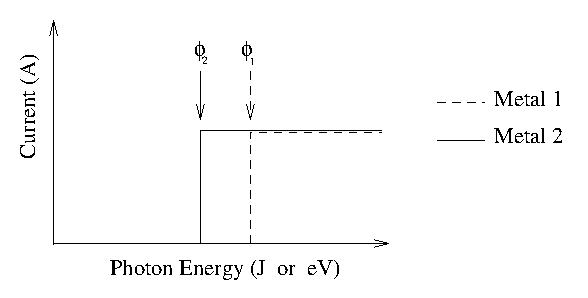
\includegraphics[width=0.6\textwidth]{../../epsimages/two_metals_2.eps}
%\caption{The current measured by the ammeter if the same light fall onto two different metals. These two metal have different work functions. %The metal with the lower work function $(\phi_{2})$ will measure a current with the ammeter at lower photon energies. This is because the %electrons need less energy to escape the surface.}
%\label{int_light_same}
%\end{center}
%\end{figure}
%\begin{figure}
%\begin{center}
%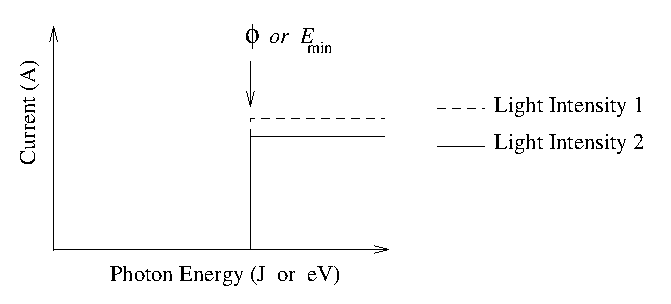
\includegraphics[width=0.6\textwidth]{../../epsimages/int_of_two_lights_2.eps}
%\caption{The current measured by the ammeter, if light of two different
%intensities falls onto the same type of metal. The greater the intensities of the light (or the greater the number of photons), the more %electrons are emitted from the metal. The emitted electrons will have the same energy for either of the two intensities. This is because the %energy of the emitted electrons depend on the energy of the photons, and not on the number of photons. }
%\label{int_light_diff}
%\end{center}
%\end{figure}

%The maximum kinetic energy acquired by the electron is equal
%to the energy of the photon minus the work function.
%The electrons emerge from the metal with a range of velocities from zero (when the photons have an energy equal to the work function) up to a
%maximum velocity $ v_{max}.$
%\begin{center}
%\psshadowbox{
%\begin{tabular}{rl}
%\multicolumn{2}{c}{ $E_{k} = hf - \phi = \frac{1}{2} m v_{max}^{2}$ } \\
%$E_{k}$ &: maximum kinetic energy of the emitted electron ($\mathrm{eV}$)\\
%$m$ &: the mass of the electron ($\mathrm{eV\cdot c^{-2}}$)\\
%$v_{max}$ &: the velocity of the emitted electron ($\mathrm{m\cdot s^{-1}}$) \\
%\end{tabular}
%}
%\end{center}

%The kinetic energy of the electron $E_k$ is directly proportional to the frequency of the radiation, and is independent of the intensity of the %light. For incoming radiation of a given frequency, the number of electrons emitted per unit time is proportional to the intensity of the %radiation. This can be shown in Fig~\ref{int_light_diff}.  The greater the intensity of the light shining on the metal, the greater the number %of electrons emitted, and hence the greater the current that is measured.
% Another important feature of the photoelectric effect, is that the electron emission takes place from the instant the light shines on the %surface, i.e. there is no detectable time delay.  This finding was unexpected. Classical theory predicted that the electrons would pick up %energy over a period of time, like the heating effect, and then be emitted. The photoelectric effect, since the electrons were emitted %instantaneously, could therefore not be explained by classical theories.  It could only be explained by assuming that each photon behaved like a %particle of light, giving all its energy instantaneously to one electron.  
%We have shown that light can act as a wave with a characteristic wavelength and frequency. This was also studied in the previous chapters on %waves \ref{chap:pw} and optics \ref{chap:optics}.  In this chapter we have studied that light can also acts as a bunch of discrete particles %each with a bundle of energy related to the frequency.  
%\begin{figure}
%\begin{center}
%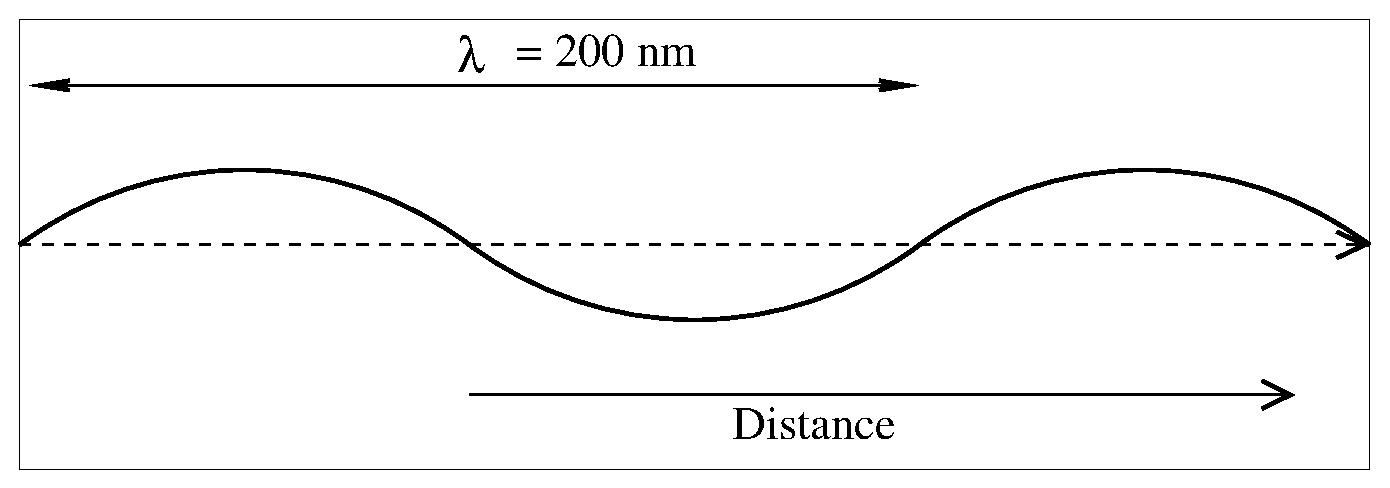
\includegraphics[width=0.4\textwidth]{../../epsimages/wave_wavelength.eps}
%\caption{Ultraviolet radiation has a wavelength of 200~nm}
%\label{int_light}
%\end{center}
%\end{figure}

%\begin{IFact}
%{It is worth mentioning that the best conductors are those with the smallest work functions. There is a very logical explanation to this. A %smaller value of the work function means that the electron is attached less strongly to its surroundings and thus it is easier for the electron %to move around inside the metal. This reduces its resistance to the flow of current.}
%\end{IFact}

\begin{wex}{The photoelectric effect - I}
{Ultraviolet radiation with a wavelength of 250~nm is incident on a silver foil (work function $\phi$ = $6,9 \times 10^{-19}$). What is the maximum kinetic energy of the emitted electrons?}
{\westep{Determine what is required and how to approach the problem}
We need to determine the maximum kinetic energy of an electron ejected from a silver foil by ultraviolet radiation. 

The photoelectric effect tells us that:
\begin{eqnarray*}
E_{k} & = & E_{photon} - \phi \\
E_k & = & h\frac{c}{\lambda}-\phi
\end{eqnarray*}

We also have: \\
Work function of silver: $\phi =6,9 \times 10^{-19}$ J  \\
UV radiation wavelength = 250~nm = $250 \times 10^{-9}$ m \\
Planck's constant: $h = 6,63 \times 10^{-34}~~\rm{m^{2}}\rm{kg}\rm{s^{-1}}$ \\
speed of light: $c = 3 \times 10^{8}~\rm{m}\rm{s^{-1}}$ \\

\westep{Solve the problem}
\begin{eqnarray*}
E_{k} & = & \frac{hc}{\lambda} - \phi \\
& = & [6,63 \times 10^{-34} \times \frac{3\times10^{8}}{250\times10^{-9}}] - 6,9 \times 10^{-19} \\
& = & 1,06 \times 10^{-19}~\rm{J}
\end{eqnarray*}

The maximum kinetic energy of the emitted electron will be $1,06 \times 10^{-19}~\rm{J}$.}
\end{wex}



\begin{wex}{The photoelectric effect - II}
{If we were to shine the same ultraviolet radiation ($f = 1,2 \times 10^{15}~\rm{Hz}$), on a gold foil (work function $= 8,2 \times 10^{-19}~\mathrm{J}$), would any electrons be emitted from the surface of the gold foil?}
{
For the electrons to be emitted from the surface, the energy of each photon needs to be \textit{greater} than the work function of the material. 
\westep{Calculate the energy of the incident photons}
\begin{eqnarray*}
E_{photon}& = & hf \\
& = & 6,63 \times 10^{-34} \times 1,2 \times 10^{15} \\
& = & 7,96 \times 10^{-19}~\rm{J}\\
\end{eqnarray*}

Therefore each photon of ultraviolet light has an energy of $7,96 \times 10^{-19}~\rm{J}$.

\westep{Write down the work function for gold.}
\begin{eqnarray*}
\phi_{gold} & = & 8,2 \times 10^{-19}~\mathrm{J} \\
\end{eqnarray*}

\westep{Is the energy of the photons greater or smaller than the work function?}

\begin{eqnarray*}
7,96 \times 10^{-19}~\rm{J} & < & 8,2 \times 10^{-19}~\mathrm{J}  \\
E_{photons} & < & \phi_{gold} \\
\end{eqnarray*}

The energy of each photon is less than the work function of gold, therefore, the photons do not have enough energy to knock electrons out of the gold. No electrons would be emitted from the gold foil.}
\end{wex}


\Extension{Units of energy}{
When dealing with calculations at a small scale (like at the level of electrons) it is more convenient to use different units for energy rather than the joule (J). We define a unit called the electron-volt (eV) as the kinetic energy gained by an electron passing through a potential difference of one volt. 
\nequ{E = q \times V}
where $q$ is the charge of the electron and $V$ is the potential difference applied. The charge of 1 electron is $1,6 \times 10^{-19}$~C, so 1~eV is calculated to be:
\nequ{1\;\mathrm{eV}= (1,6  10^{-19}\;\mathrm{C} \times 1\;\mathrm{V}) =1,6 \times 10^{-19}\eJ}

\noindent You can see that  $1,6 \times 10^{-19}$ J is a very small amount of energy and so using electron-volts (eV) at this level is easier.

\noindent Hence, 1eV = $1.6 \times 10^-19$ J which means that 1 J = $6.241 \times 10^{18}$ eV
}

%\begin{IFact}
%{Max Karl Ernst Ludwig Planck (23 April 1858 -- 4 October 1947) was one of the most  important German physicists of the late nineteenth and %early twentieth century. He is considered to be one of the founders of quantum theory. He received a Nobel prize for physics in 1918 for %recognition of the services he rendered to the advancement of Physics by his discovery of energy quanta. Planck's constant ($h$) is named after %Max Planck.}
%\end{IFact}

%\begin{IFact}
%{Albert Einstein (14 March 1879 -- 18 April 1955) was a theoretical physicist, widely regarded as the most important scientist of the twentieth %century. He made major contributions to the special and general theories of relativity and made significant contributions to quantum mechanics, %statistical mechanics, and cosmology. He was awarded the 1921 Nobel Prize for Physics for his explanation of the photoelectric effect in 1905 %and for his services to Theoretical Physics.}
%\end{IFact}

%\subsection{Relation to De Broglie's hypothesis}
%The dual-nature of light has an intricate relation with De Broglie's hypothesis. Recall that the wavelength of matter waves is given by:
%$\lambda= h/p$
%where	$\lambda$ is the wavelength of the matter wavelength, $h$ is Planck's constant and $p$ is the momentum of the body.
%De Broglie's equation gives us the wavelength of any object that has velocity (and thus momentum). Conversely, it also leads us to the idea of %electromagnetic waves possessing momentum (by just writing the equation as $p=\frac{h}{\lambda}$, where $\lambda$ is the wavelength of the %wave). This led to the idea of waves having mass, which is totally misleading. Photons do possess momentum according to several experiments, but %the existence of mass has never been established. We will assume that photons possess momentum (and not worry about whether they have mass or %not!).
 
%\begin{IFact}
%{The fact that waves have momentum has been put to some very innovative practical use. You might have heard of solar sails; several space %agencies are thinking of using them in the propulsion of space vehicles. This would use the change in momentum of light photons from the Sun %which are deflected back after striking the reflective surface of the sail. The force due to this change in momentum could be used to provide %thrust for the spacecraft.}
%\end{IFact}


\subsection{Real-life applications}
\subsubsection{Solar Cells}
The photo-electric effect may seem like a very easy way to produce electricity from the sun.
This is why people choose to make solar panels out of materials like silicon, to generate electricity. 
In real-life however, the amount of electricity generated is less than expected. This is because not every photon knocks out an electron. Other  processes such as reflection or scattering also happen. This means that only a fraction $\approx 10\%$ (depends on the material) of the photons produce photoelectrons. This drop in efficiency results in a lower current. Much work is being done in industry to improve this efficiency so that the panels can generate as high a current as possible, and create as much electricity as possible from the sun. But even these smaller electrical currents are useful in applications like solar-powered calculators.
 
\Exercise{The photoelectric effect}{
\begin{enumerate}
\item{Describe the photoelectric effect.}
\item{List two reasons why the observation of the photoelectric effect was significant.}
\item{Refer to Table~\ref{tab:work_fun}: If I shine ultraviolet light with a wavelength of 288~nm onto some aluminium foil, what would be the kinetic energy of the emitted electrons? }
\item{I shine a light of an unknown wavelength onto some silver foil. The light has only enough energy to eject electrons from the silver foil but not enough to give them kinetic energy. (Refer to Table~\ref{tab:work_fun} when answering the questions below:)
  \begin{enumerate}
  \item If I shine the same light onto some copper foil, would electrons be ejected? 
  \item If I shine the same light onto some silicon, would electrons be ejected?
  \item If I increase the intensity of the light shining on the silver foil, what happens?
  \item If I increase the frequency of the light shining on the silver foil, what happens?
  \end{enumerate} }
\end{enumerate}

% Automatically inserted shortcodes - number to insert 4
\par \practiceinfo
\par \begin{tabular}[h]{cccccc}
% Question 1
(1.)	01mq	&
% Question 2
(2.)	01mr	&
% Question 3
(3.)	01ms	&
% Question 4
(4.)	01mt	&
\end{tabular}
% Automatically inserted shortcodes - number inserted 4
}




\section{Emission and absorption spectra}

\subsection{Emission Spectra}

You have learnt previously about the structure of an atom.  The electrons surrounding the atomic nucleus are arranged in a series of levels of increasing energy.  Each element has its own distinct set of energy levels.  This arrangement of energy levels serves as the atom's unique fingerprint.
 
In the early 1900s, scientists found that a liquid or solid heated to high temperatures would give off a broad range of colours of light. However, a gas heated to similar temperatures would emit light only at certain specific colours (wavelengths).  The reason for this observation was not understood at the time.\\  
 
Scientists studied this effect using a discharge tube.  

\begin{figure}[H]
\begin{center}
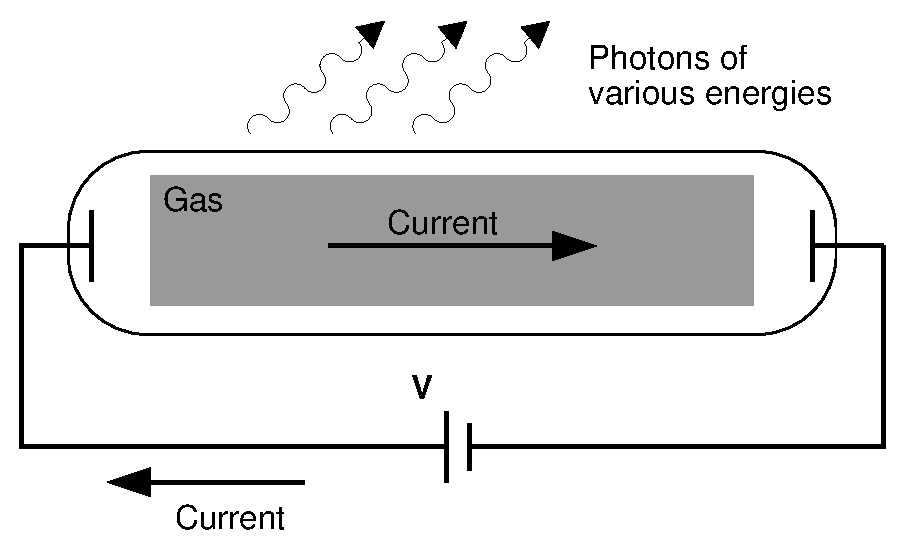
\includegraphics[width=4.in]{../../epsimages/discharge_tube.eps}
\end{center}
\caption{Diagram of a discharge tube.  The tube is filled with a gas.  When a high enough voltage is applied across the tube, the gas ionises and acts like a conductor, allowing a current to flow through the circuit.  The current excites the atoms of the ionised gas.  When the atoms fall back to their ground state, they emit photons to carry off the excess energy.}
\label{dischargetube}
\end{figure}


A discharge tube (Figure~\ref{dischargetube}) is a glass gas-filled tube with a metal plate at both ends. If a large enough voltage difference is applied between the two metal plates, the gas atoms inside the tube will absorb enough energy to make some of their electrons come off i.e. the gas atoms are ionised. These electrons start moving through the gas and create a current, which raises some electrons in other atoms to higher energy levels. Then as the electrons in the atoms fall back down, they emit electromagnetic radiation (light). The amount of light emitted at different wavelengths, called the \textbf{emission spectrum}, is shown for a discharge tube filled with hydrogen gas in figure~\ref{hydrogenspectrum} below. Only certain wavelengths (i.e. colours) of light are seen as shown by the thick black lines in the picture.

\begin{figure}[H]
\begin{center}
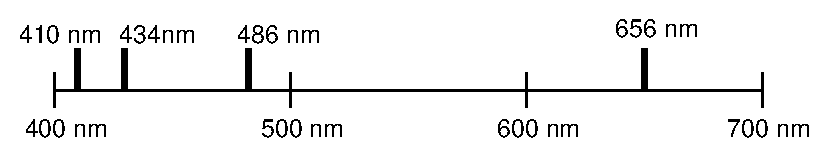
\includegraphics[width=4.5in]{../../epsimages/hydrogen_emission_spectrum.eps}
\end{center}
\caption{Diagram of the emission spectrum of hydrogen in the visible spectrum.  Four lines are visible, and are labelled with their wavelengths.  The three lines in the 400--500 nm range are in the blue part of the spectrum, while the higher line (656 nm) is in the red/orange part.}
\label{hydrogenspectrum}
\end{figure}

Eventually, scientists realised that these lines come from photons of a specific energy, emitted by electrons making transitions between specific energy levels of the atom.  Figure~\ref{ig:Henergy} shows an example of this happening.  When an electron in an atom falls from a higher energy level to a lower energy level, it emits a photon to carry off the extra energy.  This photon's energy is equal to the energy difference between the two energy levels.  As we previously discussed, the frequency of a photon is related to its energy through the equation $E=hf$.  Since a specific photon frequency (or wavelength) gives us a specific colour, we can see how each coloured line is associated with a specific transition. 
 
%\begin{figure}[H]
%\begin{center}
%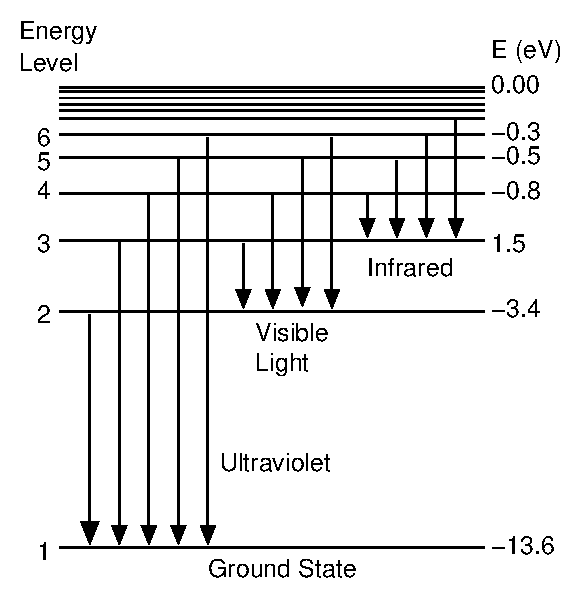
\includegraphics[width=3.5in]{../../epsimages/hydrogen_transitions.eps}
%\caption{In this diagram, various energy levels of the hydrogen atom are shown, with the associated transitions between these levels.  Each %transition gives off a photon with a distinct energy.  Each set of transitions lies in a different area of the electromagnetic spectrum.  For %example, the transitions to the ground state give off ultraviolet radiation; the transitions down to the first excited state (second energy %level) give off visible light; the transitions to the second excited state give off ultraviolet radiation.}
%\label{hydrogen-emission-diagram}
%\end{figure}

\begin{figure}[H]
\begin{center}
\scalebox{1} % Change this value to rescale the drawing.
{
\begin{pspicture}(0,-3.1)(10.66,3.1)
\psline[linewidth=0.04cm](0.7,-2.9)(7.48,-2.9)
\psline[linewidth=0.04cm](0.7,-0.08)(7.48,-0.08)
\psline[linewidth=0.04cm](0.7,0.54)(7.48,0.54)
\psline[linewidth=0.04cm](0.68,1.06)(7.46,1.06)
\psline[linewidth=0.04cm](0.66,1.54)(7.44,1.54)
\psline[linewidth=0.04cm](0.68,1.84)(7.46,1.84)
\psline[linewidth=0.04cm](0.68,2.04)(7.46,2.04)
\psline[linewidth=0.04cm](0.68,2.16)(7.46,2.16)
\psline[linewidth=0.04cm](0.68,2.26)(7.46,2.26)
\psline[linewidth=0.04cm](0.68,2.34)(7.46,2.34)
\rput(0.52,2.925){Energy}
\rput(0.49,2.605){Level}
\rput(0.51,-2.855){1}
\rput(0.51,-0.055){2}
\rput(0.52,0.545){3}
\rput(0.53,1.065){4}
\rput(0.52,1.545){5}
\rput(0.53,1.865){6}
\rput(0.51,2.345){\small $\infty$}
\rput(7.76,-2.915){\small 0 J}
\rput(8.78,-0.075){\small $16,3 \times 10^{-19}$ J}
\rput(8.8,0.565){\small $19,4 \times 10^{-19}$ J}
\rput(8.82,1.065){\small $20,5 \times 10^{-19}$ J}
\rput(8.82,1.545){\small $21,0 \times 10^{-19}$ J}
\rput(8.82,2.365){\small $21,8 \times 10^{-19}$ J}
\rput(8.84,1.825){\small $21,3 \times 10^{-19}$ J}
\psline[linewidth=0.03cm,arrowsize=0.05291667cm 2.0,arrowlength=1.4,arrowinset=0.4]{->}(1.08,-0.08)(1.1,-2.94)
\psline[linewidth=0.03cm,arrowsize=0.05291667cm 2.0,arrowlength=1.4,arrowinset=0.4]{->}(1.38,0.56)(1.4,-2.94)
\psline[linewidth=0.03cm,arrowsize=0.05291667cm 2.0,arrowlength=1.4,arrowinset=0.4]{->}(1.7,1.02)(1.7,-2.92)
\psline[linewidth=0.03cm,arrowsize=0.05291667cm 2.0,arrowlength=1.4,arrowinset=0.4]{->}(1.98,1.54)(2.0,-2.92)
\psline[linewidth=0.03cm,arrowsize=0.05291667cm 2.0,arrowlength=1.4,arrowinset=0.4]{->}(2.3,1.8)(2.32,-2.92)
\psline[linewidth=0.03cm,arrowsize=0.05291667cm 2.0,arrowlength=1.4,arrowinset=0.4]{->}(3.46,0.56)(3.48,-0.12)
\psline[linewidth=0.03cm,arrowsize=0.05291667cm 2.0,arrowlength=1.4,arrowinset=0.4]{->}(3.74,1.06)(3.74,-0.1)
\psline[linewidth=0.03cm,arrowsize=0.05291667cm 2.0,arrowlength=1.4,arrowinset=0.4]{->}(4.06,1.52)(4.06,-0.1)
\psline[linewidth=0.03cm,arrowsize=0.05291667cm 2.0,arrowlength=1.4,arrowinset=0.4]{->}(4.32,1.82)(4.36,-0.1)
\psline[linewidth=0.03cm,arrowsize=0.05291667cm 2.0,arrowlength=1.4,arrowinset=0.4]{->}(5.32,1.08)(5.34,0.46)
\psline[linewidth=0.03cm,arrowsize=0.05291667cm 2.0,arrowlength=1.4,arrowinset=0.4]{->}(5.58,1.5)(5.58,0.5)
\psline[linewidth=0.03cm,arrowsize=0.05291667cm 2.0,arrowlength=1.4,arrowinset=0.4]{->}(5.9,1.8)(5.9,0.5)
\psline[linewidth=0.03cm,arrowsize=0.05291667cm 2.0,arrowlength=1.4,arrowinset=0.4]{->}(6.22,2.0)(6.22,0.52)
\rput(3.14,-2.095){ultraviolet}
\rput(3.92,-0.395){visible light}
\rput(5.75,0.245){infrared}
\rput(9.01,-2.875){\small ground state}
\rput(8.06,2.905){Energy}
\end{pspicture} 
}
\end{center}
\caption{In this diagram are shown some of the electron energy levels for the hydrogen atom. The arrows show the electron transitions from higher energy levels to lower energy levels. The energies of the emitted photons are the same as the energy difference between two energy levels. You can think of absorption as the opposite process. The arrows would point upwards and the electrons would jump up to higher levels when they absorb a photon of the right energy.  }
\label{fig:Henergy}
\end{figure}


Visible light is not the only kind of electromagnetic radiation emitted. More energetic or less energetic transitions can produce ultraviolet or infrared radiation. However, because each atom has its own distinct set of energy levels (its fingerprint!), each atom has its own distinct emission spectrum.



 
\subsection{Absorption spectra}

As you know, atoms do not only emit photons; they also absorb photons. If a photon hits an atom and the energy of the photon is the same as the gap between two electron energy levels in the atom, then the electron can absorb the photon and jump up to the higher energy level. If the atom has no energy level differences that equal the incoming photon's energy, it cannot absorb the photon, and can only scatter it.
 
Using this effect, if we have a source of photons of various energies we can obtain the \textbf{absorption spectra} for different materials. To get an absorption spectrum, just shine white light on a sample of the material that you are interested in. White light is made up of all the different wavelengths of visible light put together. In the absorption spectrum, the energy levels corresponding to the absorbed photons show up as black lines because the photons of these wavelengths have been absorbed and don't show up. Because of this, the absorption spectrum is the exact \textit{inverse} of the emission spectrum. Look at the two figures below. In figure~\ref{fig:emissionSpec} you can see the emission lines of hydrogen. Figure~\ref{fig:absorptionSpec} shows the absorption spectrum. It is the exact opposite of the emission spectrum! Both emission and absorption techniques can be used to get the same information about the energy levels of an atom.

\begin{figure}[H]
\begin{pspicture}(\linewidth,1.1)
\psspectrum[element=H,lwidth=0.1](\linewidth,1)
\end{pspicture}
\caption{\textit{Emission} spectrum of Hydrogen.}\label{fig:emissionSpec}
\end{figure}

\begin{figure}[H]
\begin{pspicture}(\linewidth,1.1)
\psspectrum[absorption,element=H,lwidth=0.1](\linewidth,1)
\end{pspicture}
\caption{\textit{Absorption} spectrum of Hydrogen.}\label{fig:absorptionSpec}
\end{figure}



\begin{wex}{Absorption}
{I have an unknown gas in a glass container. I shine a bright white light through one side of the container and measure the spectrum of transmitted light. I notice that there is a black line (\textit{absorption} line) in the middle of the visible red band at 642 nm. I have a hunch that the gas might be hydrogen. If I am correct, between which 2 energy levels does this transition occur? (Hint: look at figure~\ref{fig:Henergy} and the transitions which are in the visible part of the spectrum.)
}
{\westep{What is given and what needs to be done?}
We have an absorption line at 642 nm. This means that the substance in the glass container absorbed photons with a wavelength of 642 nm. 
We need to calculate which 2 energy levels of hydrogen this transition would correspond to. Therefore we need to know what energy the absorbed photons had.

\westep{Calculate the energy of the absorbed photons}
\begin{eqnarray*}
E &=& \frac{hc}{\lambda} \\
  &=& \frac{(6,63 \times 10^{-34}) \times (3\times10^{8})}{642\times10^{-9}}\\
  &=& 3,1 \times 10^{-19}~~\rm{J}
\end{eqnarray*}
The absorbed photons had energy of $3,1 \times 10^{-19}$

\westep{Find the energy of the transitions resulting in radiation at visible wavelengths}
Figure~\ref{fig:Henergy} shows various energy level transitions. The transitions related to visible wavelengths are marked as the transitions beginning or ending on Energy Level 2. 
Let's find the energy of those transitions and compare with the energy of the absorbed photons we've just calculated.

Energy of transition (absorption) from Energy Level 2 to Energy Level 3:
\begin{eqnarray*}
E_{2,3} &=& E_{2} - E_{3}\\
&=& 16,3 \times 10^{-19}~~\rm{J} - 19,4 \times 10^{-19}~~\rm{J}\\
&=& -3,1 \times 10^{-19}~~\rm{J}
\end{eqnarray*}
Therefore the energy of the photon that an electron must absorb to jump from Energy Level 2 to Energy Level 3 is $3,1 \times 10^{-19}~~\rm{J}$.
(NOTE: The minus sign means that \textit{absorption} is occurring.)

This is the same energy as the photons which were absorbed by the gas in the container! Therefore, since the transitions of all elements are unique, we can say that the gas in the container is hydrogen. The transition is absorption of a photon between Energy Level 2 and Energy Level 3.

}
\end{wex}



\subsection{Colours and energies of electromagnetic radiation}
We saw in the explanation for why the sky is blue that different \textit{wavelengths} or \textit{frequencies} of light correspond to different \textit{colours} of light. The table below gives the wavelengths and colours of light in the visible spectrum:

\begin{table}[H]
\begin{center}
\begin{tabular}{ | l | c |}
\hline
\textbf{Colour} & \textbf{Wavelength range (nm)} \\ \hline \hline
 violet   & 390 - 455  \\ \hline
 blue   &   455 -  492       \\ \hline
 green  &   492 - 577        \\ \hline
 yellow  &  577 - 597       \\ \hline
 orange  &  597 - 622        \\ \hline
 red  &    622 - 780         \\ \hline
\hline
\end{tabular}
\end{center}
\caption{Colours and wavelengths of light in the visible spectrum.}
\label{t:Optic:Colours}
\end{table}

We also know that the energy of a photon of light can be found from:
\begin{eqnarray*}
E & = &hf = \frac{hc}{\lambda} 
\end{eqnarray*}
Therefore if we know the frequency or wavelength of light, we can calculate the photon's energy and vice versa. 

\Activity{Investigation}{Frequency, wavelength and energy relation}
{
\noindent Refer to table~\ref{t:Optic:Colours}: Copy the table into your workbook and add two additional columns.
\begin{enumerate}
\item In the first new column write down the lower and upper frequencies for each colour of light. 
\item In the second column write down the energy range (in Joules) for each colour of light.
\end{enumerate}
\textbf{Questions}\\
\begin{enumerate}
\item Which colour of visible light has the highest energy photons?
\item Which colour of visible light has the lowest energy photons?
\end{enumerate} 
}
Discharge lamps (sometimes incorrectly called neon lights) use the spectra of various elements to produce light of many colours.

% Phet simulation on discharge lamps: SIYAVULA-SIMULATION:http://cnx.org/content/m39553/latest/#id6358

\simulation{phet on discharge lamps}{VPqea}

\begin{wex}{Colours of light}
{A photon of wavelength 500 nm is emitted by a traffic light. 
\begin{enumerate}
\item What is the energy of the photon?
\item What is the frequency of the photon?
\item Use table~\ref{t:Optic:Colours} to determine the colour of the light.
\end{enumerate}
}
{
\westep{What information is given and what do we need to find?}
We are given $\lambda = 500 \times 10^{-9}~~\rm{m}$ and we need to find the photon's \textit{energy}, \textit{frequency} and \textit{colour}.

\westep{Use the equation $E = \frac{hc}{\lambda}$ to find the photon's energy}
\begin{eqnarray*}
E & = & \frac{hc}{\lambda} \\
& = & \frac{(6,63 \times 10^{-34}) \times (3 \times 10^{8})}{ 500 \times 10^{-9}} \\
& = & 3,98 \times 10^{-19}~~\rm{J}
\end{eqnarray*}
The energy of the photon is $3,98\times10^{-19}$ J.

\westep{We know the energy of the photon, now we can use $E=hf$ to solve for the frequency}
\begin{eqnarray*}
E & = & hf \\
f & = & \frac{E}{h} \\
  & = & \frac{3.98 \times 10^{-19}}{6,63 \times 10^{-34}}\\
  & = & 6 \times 10^{14}~~\rm{Hz}
\end{eqnarray*}
The frequency of the photon is $6 \times 10^{14}~~\rm{Hz}$.

\westep{Use the table to find the colour of light}
The wavelength given in the question is 500 nm. We can see in the table that green light has wavelengths between 492 - 577 nm. Therefore 500 nm is in this range so the colour of the light is \textbf{green}.

}
\end{wex}

\begin{wex}{Colours and energies of light}
{I have some sources which emit light of the following wavelengths:
\begin{enumerate} 
\item 400 nm, 
\item 580 nm, 
\item 650 nm,
\item 300 nm.
\end{enumerate}
What are the colours of light emitted by the sources (see table~\ref{t:Optic:Colours})? Which source emits photons with the highest energy and which with the lowest energy?
}
{
\westep{What information is given, and what do we need to do?}
Four wavelengths of light are given and we need to find their \textit{colours}. 

We also need to find which colour photon has the highest energy and which one has the lowest energy.

\westep{To find the colours of light, we can compare the wavelengths to those given in table~\ref{t:Optic:Colours}}
\begin{enumerate}
 \item 400 nm falls into the range for \textit{violet} light (390 - 455 nm).
 \item 580 nm falls into the range for \textit{yellow} light (577 - 597 nm).
 \item 650 nm falls into the range for \textit{red} light (622 - 780 nm).
 \item 300 nm is not shown in the table. However, this wavelength is just a little shorter than the shortest wavelength in the violet range. Therefore 300 nm is \textit{ultraviolet}.
\end{enumerate}

\westep{To find the colour of the light whose photons have the highest and lowest energies respectively, we need to calculate the energies of all the photons}

We know $E = \frac{hc}{\lambda}$

\begin{minipage}{0.3\textwidth}
For 400 nm:
\begin{eqnarray*}
E & = & \frac{hc}{\lambda} \\
  & = & \frac{(6,63 \times 10^{-34}) \times (3 \times 10^{8}) }{400 \times 10^{-9}} \\
  & = &  4,97 \times 10^{-19}~~\rm{J}
\end{eqnarray*}
\end{minipage}

\begin{minipage}{0.3\textwidth}
For 580 nm:
\begin{eqnarray*}
E & = & \frac{hc}{\lambda} \\
  & = & \frac{(6,63 \times 10^{-34}) \times (3 \times 10^{8}) }{580 \times 10^{-9}} \\
  & = &  3,43 \times 10^{-19}~~\rm{J}
\end{eqnarray*}
\end{minipage}

\begin{minipage}{0.3\textwidth}
For 650 nm:
\begin{eqnarray*}
E & = & \frac{hc}{\lambda} \\
  & = & \frac{(6,63 \times 10^{-34}) \times (3 \times 10^{8}) }{650 \times 10^{-9}} \\
  & = &  3,06 \times 10^{-19}~~\rm{J}
\end{eqnarray*}
\end{minipage}

\begin{minipage}{0.3\textwidth}
For 300 nm:
\begin{eqnarray*}
E & = & \frac{hc}{\lambda} \\
  & = & \frac{(6,63 \times 10^{-34}) \times (3 \times 10^{8}) }{300 \times 10^{-9}} \\
  & = &  6,63 \times 10^{-19}~~\rm{J}
\end{eqnarray*}
\end{minipage}

Therefore, the photons with the highest energy are the \textbf{ultraviolet} photons. \\
The photons with the lowest energy are from light which is \textbf{red}.

}
\end{wex}



\subsection{Applications of emission and absorption spectra}
The study of spectra from stars and galaxies in astronomy is called \textit{spectroscopy}. Spectroscopy is a tool widely used in astronomy to learn different things about astronomical objects.

\subsubsection{Identifying elements in astronomical objects using their spectra}
Measuring the spectrum of light from a star can tell astronomers what the star is made of! Since each element emits or absorbs light only at particular wavelengths, astronomers can identify what elements are in the stars from the lines in their spectra. From studying the spectra of many stars we know that there are many different types of stars which contain different elements and in different amounts.

%\textit{Nebulae} are enormous clouds of gas and dust in our galaxy which are thought to be the birth places of stars. Astronomers have been able %to deduce that most of the gas in these clouds is hydrogen gas (ionised) by identifying the emission lines in the spectra of these objects.

\subsubsection{Determining velocities of galaxies using spectroscopy}
You have already learned in Chapter~\ref{p:wsl:de12} about the Doppler effect and how the frequency (and wavelength) of sound waves changes depending on whether the object emitting the sound is moving \textit{towards} or \textit{away} from you. The same thing happens to electromagnetic radiation (light). If the object emitting the light is moving \textit{towards} us, then the wavelength of the light appears shorter (called \textbf{blue-shifted}). If the object is moving \textit{away} from us, then the wavelength of its light appears stretched out (called \textbf{red-shifted}). 

The Doppler effect affects the spectra of objects in space depending on their motion relative to us on the earth. For example, the light from a distant galaxy, which is moving away from us at some velocity, will appear red-shifted. This means that the emission and absorption lines in the galaxy's spectrum will be shifted to a longer wavelength (lower frequency). Knowing where each line in the spectrum would normally be if the galaxy was not moving, and comparing to their red-shifted positions, allows astronomers to precisely measure the velocity of the galaxy relative to the earth!



\subsubsection{Global warming and greenhouse gases}
The sun emits radiation (light) over a range of wavelengths which are mainly in the visible part of the spectrum. Radiation at these wavelengths passes through the gases of the atmosphere to warm the land and the oceans below. The warm earth then radiates this heat at longer infrared wavelengths. Carbon-dioxide (one of the main greenhouse gases) in the atmosphere has energy levels which correspond to the infrared wavelengths which allow it to absorb the infrared radiation. It then also emits at infrared wavelengths in all directions. This effect stops a large amount of the infrared radiation getting out of the atmosphere, which causes the atmosphere and the earth to heat up. More radiation is coming in than is getting back out.    

\begin{center}
\scalebox{1} % Change this value to rescale the drawing.
{
\begin{pspicture}(0,-2.59)(15.975868,2.57)
\psbezier[linewidth=0.04](3.4958684,2.53)(3.5758684,1.85)(5.2958684,1.75)(5.4158683,2.55)
\psline[linewidth=0.04cm](3.5158684,2.23)(3.1158683,1.89)
\psline[linewidth=0.04cm](3.8358684,1.99)(3.5558684,1.59)
\psline[linewidth=0.04cm](4.1958685,1.93)(4.1358685,1.47)
\psline[linewidth=0.04cm](4.5758686,1.93)(4.6358685,1.43)
\psline[linewidth=0.04cm](4.9558682,1.99)(5.1358685,1.57)
\psline[linewidth=0.04cm](5.3358684,2.21)(5.7158685,1.79)
\psbezier[linewidth=0.04,arrowsize=0.05291667cm 2.0,arrowlength=1.4,arrowinset=0.4]{->}(5.3158684,-1.8245102)(5.4166245,-1.808687)(5.439445,-1.2557855)(5.6350846,-1.3248497)(5.830724,-1.393914)(5.9961104,-1.0932733)(5.831161,-0.9905677)(5.666211,-0.8878622)(5.878371,-0.53134257)(6.0578475,-0.6263778)(6.2373247,-0.7214131)(6.42343,-0.38185132)(6.2439528,-0.28681606)(6.064476,-0.19178078)(6.281192,0.17768885)(6.4606686,0.082653575)(6.640146,-0.012381695)(6.358866,-0.0017902247)(6.759594,0.57)
\psbezier[linewidth=0.03,arrowsize=0.05291667cm 2.0,arrowlength=1.4,arrowinset=0.4]{->}(4.266691,1.9676449)(4.4793305,1.9886502)(4.4655175,1.7896867)(4.310693,1.7585212)(4.1558685,1.7273557)(4.168905,1.5119989)(4.3296576,1.5552567)(4.4904103,1.5985147)(4.5284834,1.3772986)(4.3832135,1.3371572)(4.237943,1.2970159)(4.2414255,1.090635)(4.4099193,1.1354511)(4.578413,1.1802672)(4.579593,0.9407257)(4.455734,0.9157933)(4.331874,0.89086086)(4.3371696,0.6739458)(4.5015483,0.69613546)(4.665927,0.71832514)(4.6848917,0.5150607)(4.530067,0.4838952)(4.3752427,0.4527297)(4.40969,0.2525818)(4.5740685,0.2747715)(4.738447,0.2969612)(4.72826,0.07692955)(4.579364,0.05785641)(4.4304676,0.03878328)(4.48221,-0.16878216)(4.6311064,-0.14970903)(4.7800026,-0.13063589)(4.8203783,-0.3186914)(4.667367,-0.36039102)(4.514355,-0.4020906)(4.564285,-0.5991219)(4.709555,-0.55898064)(4.8548255,-0.5188393)(4.90064,-0.7384971)(4.7458153,-0.7696626)(4.590991,-0.8008281)(4.6368055,-1.0204859)(4.79163,-0.9893204)(4.9464545,-0.9581549)(4.967232,-1.1719534)(4.818336,-1.1910266)(4.6694393,-1.2100997)(4.7307363,-1.426641)(4.8700786,-1.398592)(5.0094204,-1.370543)(5.022457,-1.5858998)(4.883115,-1.6139488)(4.743773,-1.6419978)(4.908641,-1.5761135)(4.955779,-1.85)
\pscircle[linewidth=0.03,dimen=outer](6.8258686,0.62){0.05}
\pscircle[linewidth=0.03,dimen=outer](7.0258684,0.42){0.05}
\pscircle[linewidth=0.03,dimen=outer](6.8458686,0.5){0.05}
\pscircle[linewidth=0.03,dimen=outer](6.6858683,0.62){0.05}
\psbezier[linewidth=0.04,arrowsize=0.05291667cm 2.0,arrowlength=1.4,arrowinset=0.4]{->}(6.8915195,0.5453803)(6.9068,0.44454044)(7.4595704,0.41874084)(7.389453,0.22347647)(7.3193355,0.028212115)(7.619081,-0.13879196)(7.7226734,0.025601879)(7.8262663,0.18999572)(8.181638,-0.024081578)(8.085637,-0.20304397)(7.989636,-0.38200638)(8.32819,-0.5699386)(8.4241905,-0.39097622)(8.520192,-0.21201381)(8.888489,-0.43071732)(8.792487,-0.6096797)(8.696486,-0.7886421)(8.708593,-0.5074236)(9.278216,-0.91122675)
\psbezier[linewidth=0.03,arrowsize=0.05291667cm 2.0,arrowlength=1.4,arrowinset=0.4]{->}(0.6758684,-2.49)(2.0158684,-1.89)(8.495869,-1.33)(11.615869,-2.45)
\psbezier[linewidth=0.04,arrowsize=0.05291667cm 2.0,arrowlength=1.4,arrowinset=0.4]{->}(2.3639035,0.53901273)(2.3501835,0.64007664)(1.7978777,0.67441475)(1.8710039,0.8685723)(1.9441302,1.0627298)(1.6470013,1.2343458)(1.5408807,1.0715723)(1.43476,0.9087988)(1.082739,1.1283418)(1.1814939,1.3057994)(1.2802488,1.483257)(0.9446391,1.6763983)(0.8458842,1.4989406)(0.7471294,1.321483)(0.38225624,1.5458515)(0.4810111,1.723309)(0.579766,1.9007666)(0.56331503,1.6197687)(0.0,2.0323257)
\psbezier[linewidth=0.04,arrowsize=0.05291667cm 2.0,arrowlength=1.4,arrowinset=0.4]{->}(3.6348133,-1.9369571)(3.671527,-1.8418032)(3.204232,-1.5453975)(3.3619184,-1.4105656)(3.5196047,-1.2757337)(3.3420558,-0.9821116)(3.1705978,-1.0735391)(2.99914,-1.1649667)(2.796613,-0.8028884)(2.9686987,-0.6950449)(3.1407845,-0.58720136)(2.9399037,-0.25616616)(2.767818,-0.3640097)(2.5957322,-0.47185323)(2.3842728,-0.09935028)(2.5563583,0.008493258)(2.728444,0.1163368)(2.5785341,-0.121901385)(2.2839727,0.5111552)
\psbezier[linewidth=0.03,arrowsize=0.05291667cm 2.0,arrowlength=1.4,arrowinset=0.4]{->}(4.0897393,2.0019855)(4.2958684,1.958283)(4.2253532,1.7663379)(4.0706806,1.7825129)(3.9160075,1.7986879)(3.866014,1.5824502)(4.02976,1.5763997)(4.1935062,1.5703491)(4.165374,1.340752)(4.017095,1.345185)(3.8688161,1.3496181)(3.8124285,1.1451223)(3.9839082,1.138263)(4.155388,1.1314037)(4.087248,0.89491713)(3.9635096,0.9078571)(3.8397713,0.9207971)(3.7820442,0.70536816)(3.9431107,0.67745125)(4.1041775,0.6495343)(4.063257,0.44342107)(3.9085844,0.45959604)(3.7539117,0.47577104)(3.7284586,0.2680403)(3.8895254,0.24012335)(4.050592,0.21220641)(3.9773977,-0.0016050348)(3.831798,0.024694402)(3.6861987,0.050993837)(3.674873,-0.1692876)(3.8204727,-0.19558704)(3.966072,-0.22188649)(3.9496922,-0.41949278)(3.79368,-0.414251)(3.6376677,-0.4090092)(3.6276817,-0.6183574)(3.7759604,-0.6227905)(3.9242392,-0.62722355)(3.9038405,-0.8576294)(3.749168,-0.84145445)(3.594495,-0.8252794)(3.5740964,-1.0556853)(3.728769,-1.0718603)(3.883442,-1.0880353)(3.8411818,-1.3050817)(3.6955824,-1.2787824)(3.5499828,-1.2524829)(3.5450516,-1.4845062)(3.684257,-1.4990637)(3.8234625,-1.5136212)(3.7734687,-1.729859)(3.6342633,-1.7153015)(3.4950578,-1.700744)(3.6692169,-1.6857369)(3.6343863,-1.97)
\pscircle[linewidth=0.03,dimen=outer](2.3658683,0.56){0.05}
\pscircle[linewidth=0.03,dimen=outer](2.2258685,0.56){0.05}
\rput(5.9658685,-2.365){earth radiates long wavelength infrared radiation}
\rput(10.715868,2.275){\small the sun emits short wavelength radiation which penetrates the atmosphere}
\rput(10.155869,0.835){\small CO$_{2}$ molecules absorb and re-emit}
\rput(9.905869,0.535){\small the infrared radiation in all directions}
\rput(9.255868,0.235){\small heating the atmosphere}
\end{pspicture} 
}
\end{center}

Therefore increasing the amount of greenhouse gases in the atmosphere increases the amount of trapped infrared radiation and therefore the overall temperature of the earth. The earth is a very sensitive and complicated system upon which life depends and changing the delicate balances of temperature and atmospheric gas content may have disastrous consequences if we are not careful. 

\Activity{Investigation}{The greenhouse effect}
{\noindent In pairs try to find the following information (e.g. in books, on the internet) and report back to the class in a 5 minute presentation which includes the following:
\begin{enumerate}
\item What other gases besides carbon dioxide are responsible for the greenhouse effect?
\item Where do greenhouse gases come from? (are they human-made or natural?)
\item Investigate one serious side-effect which could arise if the earth's temperature were to go up significantly. Present some ways in which this effect could be avoided.
\end{enumerate}
}




\Exercise{Emission and absorption spectra}{
\begin{enumerate}
\item Explain how atomic emission spectra arise and how they relate to each element on the periodic table.
\item How do the lines on the atomic spectrum relate to electron transitions between energy levels?
\item Explain the difference between atomic absorption and emission spectra.
\item Describe how the absorption and emission spectra of the gases in the atmosphere give rise to the Greenhouse Effect. 

\item Using table~\ref{t:Optic:Colours} calculate the frequency range for yellow light.
\item What colour is the light emitted by hydrogen when an electron makes the transition from energy level 5 down to energy level 2? (Use figure~\ref{fig:Henergy} to find the energy of the released photon.)
\item I have a glass tube filled with hydrogen gas. I shine white light onto the tube. The spectrum I then measure has an absorption line at a wavelength of 474 nm. Between which two energy levels did the transition occur? (Use figure~\ref{fig:Henergy} in solving the problem.)
\end{enumerate}

% Automatically inserted shortcodes - number to insert 7
\par \practiceinfo
\par \begin{tabular}[h]{cccccc}
% Question 1
(1.)	01mu	&
% Question 2
(2.)	01mv	&
% Question 3
(3.)	01mw	&
% Question 4
(4.)	01mx	&
% Question 5
(5.)	01my	&
% Question 6
(6.)	01mz	\\ % End row of shortcodes
% Question 7
(7.)	01n0	&
\end{tabular}
% Automatically inserted shortcodes - number inserted 7
}



\section{Lasers}

%\begin{syllabus}
%\item This section should contain the following to enable learners to explain and contrast the concepts of spontaneous emission of radiation and stimulated emission of radiation.
%\item State that Lasers emit light which is monochromatic and in phase.
%\item Explain - in simple terms - how a laser works. Include concepts of a meta-stable state, population inversion and the consequence of decay of some atoms from the meta-stable state and their subsequent stimulation of other excited atoms to emit photons in phase with this emission.

%\item Recognise that the materials used for Lasers all allow a population inversion to be set up and that materials which have been used include synthetic ruby, a mixture of helium and neon (He-Ne lasers) and various semiconductors.
%\item Describe the arrangement of the Laser cavity and its effects of:
%\begin{itemize}
%\item Increasing amplification
%\item Concentrating beam intensity
%\item Improving the spectral purity of the beam (Narrowing the frequency of the beam.)
%\end{itemize}
%\item Identify some advantages of Laser applications in respect of:
%\begin{itemize}
%\item Barcodes
%\item Laser communication and Fibre-optics
%\item Medical Lasers
%\item Laser printers
%\item Optical storage media
%\end{itemize}
%\item In the Real-World: Include applications of the content in this chapter to the following to highlight applications in the real world
%\begin{itemize}
%\item chemistry in the home;
%\item science in fashion;
%\item medical and industrial uses of lasers;
%\item astrophysics;
%\item civil engineering.
%\end{itemize}
%\end{syllabus}

A laser is a device that produces a special type of light: all the laser photons are identical! They all have the \textit{same} wavelength (and frequency), amplitude and phase. Since they all have the same wavelength, this means they all have the same \textit{colour} and the light is called \textbf{monochromatic}. (\textit{Note:} \textit{mono} means "one" or "single" and \textit{chromatic} means "colour".) This is very different to most other light sources which produce light with a range of wavelengths (e.g. white light from the sun consists of all the visible wavelengths.)
 
Laser light is highly directional and can be focused very well. This focus allows laser beams to be used over long distances, and to pack a lot of energy into the beam while still requiring reasonably small amounts of energy to be generated. Each centimetre of a typical laser beam contains many billions of photons. 
These special properties of laser light come from the way in which the laser photons are created and the energy levels of the material that makes up the laser. These properties make laser light extremely useful in many applications from CD players to eye surgery.\\
 
The term \textbf{LASER} stands for \textbf{L}ight \textbf{A}mplification by the \textbf{S}timulated \textbf{E}mission of \textbf{R}adiation. This \textbf{stimulated emission} is different to the \textbf{spontaneous emission} already discussed earlier. Let's review the absorption and emission processes which can occur in atoms.

\begin{center}
\scalebox{1} % Change this value to rescale the drawing.
{
\begin{pspicture}(0,-3.32)(15.88,3.32)
\definecolor{color1765}{rgb}{0.6,0.6,0.6}
\psline[linewidth=0.04cm](1.78,2.62)(4.42,2.62)
\psline[linewidth=0.04cm](1.78,1.8)(4.42,1.8)
\psline[linewidth=0.04cm](1.8,0.34)(4.44,0.34)
\psline[linewidth=0.04cm](1.8,-0.48)(4.44,-0.48)
\psline[linewidth=0.04cm](1.78,-2.06)(4.42,-2.06)
\psline[linewidth=0.04cm](1.78,-2.88)(4.42,-2.88)
\psline[linewidth=0.04cm](7.14,2.62)(9.78,2.62)
\psline[linewidth=0.04cm](7.14,1.8)(9.78,1.8)
\psline[linewidth=0.04cm](7.16,0.34)(9.8,0.34)
\psline[linewidth=0.04cm](7.16,-0.48)(9.8,-0.48)
\psline[linewidth=0.04cm](7.14,-2.06)(9.78,-2.06)
\psline[linewidth=0.04cm](7.14,-2.88)(9.78,-2.88)
\rput(3.09,3.125){BEFORE}
\rput(8.42,3.125){AFTER}
\psbezier[linewidth=0.04,arrowsize=0.05291667cm 2.0,arrowlength=1.4,arrowinset=0.4]{->}(0.056190476,2.188395)(0.04,2.0696297)(0.26666668,2.06)(0.26666668,2.188395)(0.26666668,2.31679)(0.5257143,2.31679)(0.5095238,2.188395)(0.49333334,2.06)(0.68761903,2.06)(0.68761903,2.188395)(0.68761903,2.31679)(0.8657143,2.31679)(0.8657143,2.188395)(0.8657143,2.06)(1.0438095,2.0632098)(1.0438095,2.1916049)(1.0438095,2.32)(1.2057143,2.31679)(1.1895238,2.1916049)(1.1733333,2.0664198)(1.176,2.2044444)(1.4,2.1916049)
\pscircle[linewidth=0.04,dimen=outer,fillstyle=solid,fillcolor=black](3.11,1.81){0.09}
\pscircle[linewidth=0.04,dimen=outer,fillstyle=solid,fillcolor=black](8.49,2.61){0.09}
\rput(1.58,1.8){\footnotesize E1}
\rput(1.58,2.64){\footnotesize E2}
\rput(1.6,0.36){\footnotesize E2}
\rput(1.6,-0.48){\footnotesize E1}
\rput(1.58,-2.08){\footnotesize E2}
\rput(1.58,-2.92){\footnotesize E1}
\rput(6.94,0.34){\footnotesize E2}
\rput(6.94,-0.5){\footnotesize E1}
\rput(6.92,-2.06){\footnotesize E2}
\rput(6.92,-2.9){\footnotesize E1}
\rput(6.94,2.64){\footnotesize E2}
\rput(6.94,1.8){\footnotesize E1}
\rput(10.4,2.22){\footnotesize no photon}
\rput(5.64,2.225){\textit{absorption}}
\rput(5.69,0.125){\textit{spontaneous}}
\rput(5.61,-0.215){\textit{emission}}
\rput(5.63,-2.335){\textit{stimulated}}
\rput(5.59,-2.675){\textit{emission}}
\pscircle[linewidth=0.04,dimen=outer,fillstyle=solid,fillcolor=black](3.13,0.35){0.09}
\pscircle[linewidth=0.04,dimen=outer,fillstyle=solid,fillcolor=black](8.45,-0.47){0.09}
\psbezier[linewidth=0.04,arrowsize=0.05291667cm 2.0,arrowlength=1.4,arrowinset=0.4]{->}(9.856191,-0.11160494)(9.84,-0.23037037)(10.066667,-0.24)(10.066667,-0.11160494)(10.066667,0.016790124)(10.325714,0.016790124)(10.309524,-0.11160494)(10.293333,-0.24)(10.487619,-0.24)(10.487619,-0.11160494)(10.487619,0.016790124)(10.665714,0.016790124)(10.665714,-0.11160494)(10.665714,-0.24)(10.843809,-0.23679012)(10.843809,-0.10839506)(10.843809,0.02)(11.005714,0.016790124)(10.989524,-0.10839506)(10.973333,-0.23358025)(10.976,-0.09555556)(11.2,-0.10839506)
\rput(0.65,2.425){\scriptsize E=E2-E1}
\rput(10.49,0.105){\scriptsize E=E2-E1}
\psbezier[linewidth=0.04,arrowsize=0.05291667cm 2.0,arrowlength=1.4,arrowinset=0.4]{->}(0.07619048,-2.571605)(0.06,-2.6903703)(0.28666666,-2.7)(0.28666666,-2.571605)(0.28666666,-2.44321)(0.54571426,-2.44321)(0.5295238,-2.571605)(0.5133333,-2.7)(0.7076191,-2.7)(0.7076191,-2.571605)(0.7076191,-2.44321)(0.8857143,-2.44321)(0.8857143,-2.571605)(0.8857143,-2.7)(1.0638095,-2.6967902)(1.0638095,-2.5683951)(1.0638095,-2.44)(1.2257143,-2.44321)(1.2095238,-2.5683951)(1.1933334,-2.6935802)(1.196,-2.5555556)(1.42,-2.5683951)
\rput(0.67,-2.335){\scriptsize E=E2-E1}
\pscircle[linewidth=0.04,dimen=outer,fillstyle=solid,fillcolor=black](3.09,-2.05){0.09}
\pscircle[linewidth=0.04,dimen=outer,fillstyle=solid,fillcolor=black](8.43,-2.87){0.09}
\psbezier[linewidth=0.04,arrowsize=0.05291667cm 2.0,arrowlength=1.4,arrowinset=0.4]{->}(9.856191,-2.571605)(9.84,-2.6903703)(10.066667,-2.7)(10.066667,-2.571605)(10.066667,-2.44321)(10.325714,-2.44321)(10.309524,-2.571605)(10.293333,-2.7)(10.487619,-2.7)(10.487619,-2.571605)(10.487619,-2.44321)(10.665714,-2.44321)(10.665714,-2.571605)(10.665714,-2.7)(10.843809,-2.6967902)(10.843809,-2.5683951)(10.843809,-2.44)(11.005714,-2.44321)(10.989524,-2.5683951)(10.973333,-2.6935802)(10.976,-2.5555556)(11.2,-2.5683951)
\rput(10.51,-2.855){\scriptsize E=E2-E1}
\psbezier[linewidth=0.04,arrowsize=0.05291667cm 2.0,arrowlength=1.4,arrowinset=0.4]{->}(9.856191,-2.331605)(9.84,-2.4503703)(10.066667,-2.46)(10.066667,-2.331605)(10.066667,-2.2032099)(10.325714,-2.2032099)(10.309524,-2.331605)(10.293333,-2.46)(10.487619,-2.46)(10.487619,-2.331605)(10.487619,-2.2032099)(10.665714,-2.2032099)(10.665714,-2.331605)(10.665714,-2.46)(10.843809,-2.4567902)(10.843809,-2.3283951)(10.843809,-2.2)(11.005714,-2.2032099)(10.989524,-2.3283951)(10.973333,-2.4535801)(10.976,-2.3155556)(11.2,-2.3283951)
\rput(10.49,-2.115){\scriptsize E=E2-E1}
\rput[l](11.43,2.765){\small a photon with E=E2-E1 }
\rput[l](11.43,2.125){\small which jumps from energy }
\rput[l](11.43,1.785){\small level E1 to E2}
\rput[l](11.43,0.425){\small an electron on energy }
\rput[l](11.43,-0.175){\small drop down to energy level}
\rput[l](11.43,-0.515){\small E1 by emitting a photon with }
\rput[l](11.43,-1.875){\small an electron on energy level}
\rput[l](11.43,-2.495){\small incoming photon with E=E2-E1}
\rput[l](11.43,-3.095){\small another photon of E=E2-1}
\rput[l](11.43,-2.815){\small to drop down to E1 by emitting }
\rput(0.76,-0.1){\footnotesize no photon}
\rput[l](11.43,2.445){\small is absorbed by the electron}
\rput[l](11.43,0.125){\small level E2 can spontaneously}
\rput[l](11.43,-0.875){\small E=E2-E1}
\rput[l](11.43,-2.215){\small E2 can be stimulated, by an}
\psline[linewidth=0.04cm,linecolor=color1765,linestyle=dashed,dash=0.16cm 0.16cm](0.02,1.06)(15.42,1.06)
\psline[linewidth=0.04cm,linecolor=color1765,linestyle=dashed,dash=0.16cm 0.16cm](0.0,-1.36)(15.4,-1.36)
\end{pspicture} 
}

\end{center}

\begin{itemize}
\item \textbf{Absorption}: As you can see in the picture above, \textbf{absorption} happens when an electron jumps up to a higher energy level by \textit{absorbing} a photon which has an energy equal to the energy difference between the two energy levels. 

\item \textbf{Spontaneous emission}: \textbf{Spontaneous emission} is when an electron in a higher energy level drops down to a lower energy level and a photon is emitted with an energy equal to the energy difference between the two levels. There is no interference in this process from outside factors. Usually spontaneous emission happens very quickly after an electron gets into an excited state. In other words, the lifetime of the excited state is very short (the electron only stays in the high energy level for a very short time). However, there are some excited states where an electron can remain in the higher energy level for a longer time than usual before dropping down to a lower level. These excited states are called \textbf{metastable states.}

\item \textbf{Stimulated emission}: As the picture above shows, \textbf{stimulated emission} happens when a photon with an energy equal to the energy difference between two levels interacts with an electron in the higher level. This \textit{stimulates} the electron to emit an identical photon and drop down to the lower energy level. This process results in two photons at the end.

\end{itemize}

\Definition{Spontaneous Emission}{Spontaneous emission occurs when an atom is in an unstable excited state and randomly decays to a less energetic state, emitting a photon to carry off the excess energy.  The unstable state decays in a characteristic time, called the lifetime.}

\Definition{Meta-stable state}{A meta-stable state is an excited atomic state that has an unusually long lifetime, compared to the lifetimes of other excited states of that atom. While most excited states have lifetimes measured in microseconds and nanoseconds ($10^{-6}$ s and $10^{-9}$ s), meta-stable states can have lifetimes of milliseconds ($10^{-3}$ s) or even seconds.}

\Definition{Stimulated emission}{Stimulated emission occurs when a photon interacts with an excited atom,  causing the atom to decay and emit another identical photon.}


\subsection{How a laser works}
A laser works by a process called \textit{stimulated emission} - as you can tell from what `laser' stands for! 
You can imagine that stimulated emission can lead to more and more identical photons being released in the following way: Imagine we have an electron in an excited metastable state and it drops down to the ground state by emitting a photon. If this photon then travels through the material and meets another electron in the metastable excited state this will cause the electron to drop down to the lower energy level and another photon to be emitted. Now there are two photons of the same energy. If these photons then both move through the material and \textit{each} interacts with another electron in a metastable state, this will result in them \textit{each} causing an additional photon to be released. i.e. from 2 photons we then get 4, and so on! This is how laser light is produced.

\begin{figure}[!h]
\begin{center}
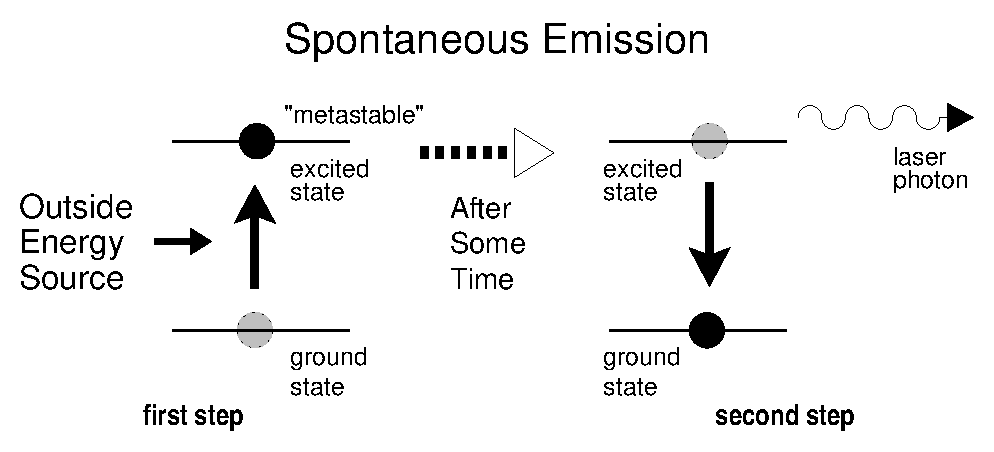
\includegraphics[width=5.in]{../../epsimages/laser-spontaneous_2.eps}
\end{center}
\caption{Spontaneous emission is a two step process, as shown here.  First, energy from an external source is applied to an atom in the laser medium, raising its energy to an excited (metastable) state.  After some time, it will decay back down to its ground state and emit the excess energy in the form of a photon.  This is the first stage in the formation of a laser beam. }
\label{laserse}
\end{figure}

\begin{figure}[!h]
\begin{center}
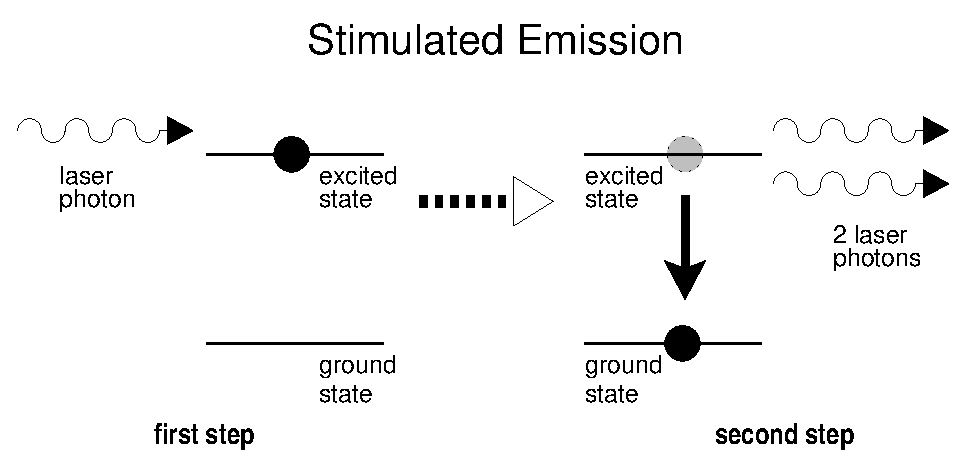
\includegraphics[width=5.in]{../../epsimages/laser-amplification_2.eps}
\end{center}
\caption{Stimulated emission is also a two step process, as shown here.  First, a laser photon encounters an atom that has been raised to an excited state, just like in the case of spontaneous emission.  The photon then causes the atom to decay to its ground state and emit another photon identical to the incoming photon.  This is the second step in the creation of a laser beam.  It happens many, many times as the laser photons pass through the optical cavity until the laser beam builds up to full strength.}
\label{laseramp}
\end{figure}


This can only happen if there are many electrons in a metastable state. If most of the electrons are in the ground state, then they will just \textit{absorb} the photons and no extra photons will be emitted. However, if more electrons are in the excited metastable state than in the ground state, then the process of stimulated emission will be able to continue. Usually in atoms, most of the electrons are in the lower energy levels and only a few are in excited states. When most of the electrons are in the excited metastable state and only a few are in the ground state, this is called \textbf{population inversion} (the populations in the excited and ground states are \textit{swapped} around) and this is when stimulated emission can occur. To start off the process, the electrons first have to be excited up into the metastable state. This is done using an external energy source.


\Definition{Population inversion}{Population inversion is when more atoms are in an excited state than in their ground state. It is a necessary condition to sustain a laser beam, so that there are enough excited atoms that can be stimulated to emit more photons.}


\begin{center}
\scalebox{1} % Change this value to rescale the drawing.
{
\begin{pspicture}(0,-1.46)(10.32,1.46)
\psline[linewidth=0.04cm](1.6,1.2)(4.42,1.2)
\psline[linewidth=0.04cm](1.6,-0.16)(4.42,-0.16)
\rput(0.77,-0.14){\footnotesize ground state}
\rput(0.76,1.3){\footnotesize metastable}
\rput(0.76,1.02){\footnotesize state}
\psline[linewidth=0.04cm](6.68,1.2)(9.5,1.2)
\psline[linewidth=0.04cm](6.68,-0.16)(9.5,-0.16)
\rput(5.85,-0.14){\footnotesize ground state}
\rput(5.84,1.3){\footnotesize metastable}
\rput(5.84,1.02){\footnotesize state}
\psdots[dotsize=0.12](2.16,-0.16)
\psdots[dotsize=0.12](2.36,-0.16)
\psdots[dotsize=0.12](2.58,-0.16)
\psdots[dotsize=0.12](2.8,-0.16)
\psdots[dotsize=0.12](3.02,-0.16)
\psdots[dotsize=0.12](3.24,-0.16)
\psdots[dotsize=0.12](3.46,-0.16)
\psdots[dotsize=0.12](3.66,-0.16)
\psdots[dotsize=0.12](7.26,1.18)
\psdots[dotsize=0.12](7.46,1.18)
\psdots[dotsize=0.12](7.68,1.18)
\psdots[dotsize=0.12](7.9,1.18)
\psdots[dotsize=0.12](8.12,1.18)
\psdots[dotsize=0.12](8.34,1.18)
\psdots[dotsize=0.12](8.56,1.18)
\psdots[dotsize=0.12](8.76,1.18)
\psdots[dotsize=0.12](2.68,1.18)
\psdots[dotsize=0.12](3.06,1.2)
\psdots[dotsize=0.12](3.46,1.18)
\psdots[dotsize=0.12](7.6,-0.18)
\psdots[dotsize=0.12](7.98,-0.16)
\psdots[dotsize=0.12](8.38,-0.18)
\rput(2.1,-0.915){usually most electrons are in }
\rput(7.65,-0.895){most electrons in excited metastable}
\rput(7.66,-1.235){state = \textit{population inversion}}
\rput(1.18,-1.215){the ground state}
\end{pspicture} 
}
\end{center}

Therefore, materials used to make laser light \textit{must} must have metastable states which can allow population inversion to occur when an external energy source is applied. Some substances which are used to make lasers are listed in table~\ref{lasertypes}. You can see that gases (such as Helium-Neon mixture), liquids (such as dyes), and solids (such as the precious stone ruby) are all used to make lasers. 


\begin{table}[H]
\begin{center}
\begin{tabular}{lccl}
\hline
\textbf{Material} & \textbf{Type} & \textbf{Wavelength} & \textbf{Uses} \\
\hline
Helium--Neon & gas & 632,8 nm & scientific research, holography \\
%Argon ion & gas & 488.0 nm, 514.5 nm & medicine, \\
%Carbon dioxide & gas & 10.6 $\mu$m, 9.4 $\mu$m & industry (cutting, welding), surgery \\
%Helium--Cadmium & vapor & 440 nm, 325 nm & printing, scientific research \\
Argon ion & gas & 488,0 nm & medicine, \\
Carbon dioxide & gas & 10,6 $\mu$m & industry (cutting, welding), surgery \\
Helium--Cadmium & vapour & 325 nm & printing, scientific research \\
Ruby & solid--state & 694,3 nm & holography \\
Neodymium YAG & solid--state & 1,064 $\mu$m & industry, surgery, research \\
(Yttrium Aluminium \\
Garnet) \\
Titanium--Sapphire & solid--state & 650--1100 nm & research \\
Laser diode & semiconductor & 375--1080 nm & telecommunications, industry, \\
& & & printing, CD players, laser pointers \\
\hline
\end{tabular}
\end{center}
\caption{A selection of different lasers. The laser material and general type of each laser is given, along with typical wavelengths of the laser light they create. Examples of real-world applications are also given. All these materials allow a population inversion to be set up.}
\label{lasertypes}
\end{table}


\begin{IFact}
{The first working laser, using synthetic ruby as the laser material, was made by Theodore H. Maiman at Hughes Research Laboratories in Malibu, California. Later in the same year the Iranian physicist Ali Javan, together with William Bennet and Donald Herriot, made the first gas laser using helium and neon. Javan received the Albert Einstein Award in 1993.}
\end{IFact}


\subsection{A simple laser}


A laser consists of a number of different parts that work together to create the laser beam.  Figure~\ref{lasercavity} shows the different parts of the laser, while Figure~\ref{laserprocess} shows how they create the laser beam.\\

\begin{figure}[!htb]
\begin{center}
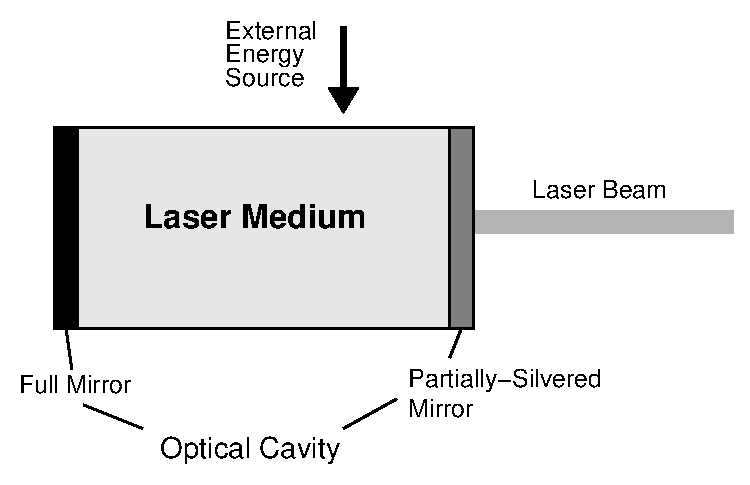
\includegraphics[width=4.8in]{../../epsimages/laser-cavity_2.eps}
\end{center}
\caption{Diagram of a laser showing the main components.}
\label{lasercavity}
\end{figure}


\begin{figure}[!tb]
\begin{center}
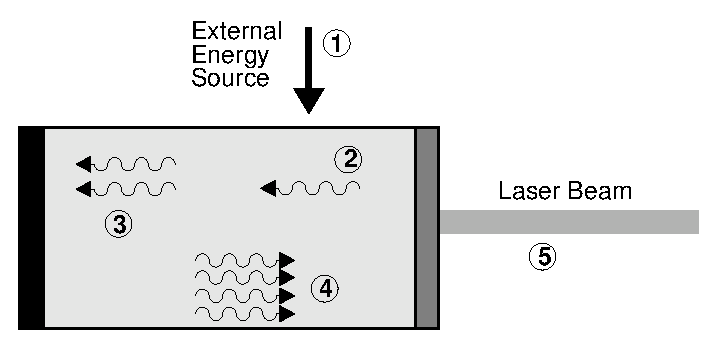
\includegraphics[width=4.5in]{../../epsimages/laser-process.eps}
\end{center}
\caption{Diagram of a laser showing the process of creating a laser beam. (1) A source of external energy is applied to the laser medium, raising the atoms to an excited state. (2) An excited atom decays though spontaneous emission, emitting a photon.  (3) The photon encounters another excited atom and causes it to decay through stimulated emission, creating another photon. (4) The photons bounce back and forth through the laser medium between the mirrors, building up more and more photons.  (5) A small percentage of the photons pass through the partially-silvered mirror to become the laser beam we see.}
\label{laserprocess}
\end{figure}
 
The basis of the laser is the laser material which consists of the atoms that are used to create the laser beam. Many different materials can be used as laser material, and their energy levels determine the characteristics of the laser. Some examples of different lasers are shown in Table~\ref{lasertypes}. The laser material is contained in the optical cavity.\\ 
 
Before the laser is turned on, all the atoms in the laser material are in their ground state. The first step in creating a laser beam is to add energy to the laser material to raise most of the electrons into an excited metastable state. This is called \textit{pumping} the laser. \\ 

The creation of the laser beam starts through the process of \textit{spontaneous emission}, shown in Figure~\ref{laserse}. An electron drops down to the ground state and emits a photon with energy equal to the energy difference of the two energy levels. This laser photon is the beginning of the laser beam.\\

At some time a laser photon will run into another excited electron. Then stimulated emission occurs and the electron drops down to the ground state and emits an additional identical photon as shown in Figure~\ref{laseramp}. Since the laser material typically has a large number of atoms, one laser photon passing through this material will rapidly cause a large number of photons just like it to be emitted.\\
 
The optical cavity keeps the laser photons inside the laser cavity so that they can build up the laser beam. At each end is a concave mirror; one is a full mirror and one is a partial mirror. The full mirror is totally reflective. The partial mirror transmits a small amount of the light that hits it (less than 1\%). The mirrors are carefully aligned so that photons that reflect off one mirror become ``trapped'', and bounce back and forth between the mirrors many times causing more and more stimulated emission. The photons that eventually escape through the partially-silvered mirror become the laser beam that we see.\\
 
As the photons bounce between mirrors, they continually pass through the laser material, stimulating those atoms to emit more photons.  This creates an ever increasing beam of photons, all with the same characteristics, all travelling in the same direction.  In this way, the optical cavity helps to amplify the original laser photons into a concentrated, intense beam of photons.\\

The laser cavity also helps to narrow the frequency range of laser light emitted. The distance between the two mirrors defines the cavity \textit{mode} which only allows light of a narrow range of frequencies to continue being reflected back and forth. Light of other frequencies damped out. (This is just like in the chapter on the physics of music where a pipe of a certain length corresponds to a particular wavelength of sound.) Therefore only a narrow frequency of light can be emitted.


\begin{IFact}
{In 1953, Charles H. Townes and graduate students James P. Gordon and Herbert J. Zeiger produced the first maser, a device operating on similar principles to the laser, but producing microwave rather than optical radiation. Townes's maser was incapable of making a continuous beam. Nikolay Basov and Aleksandr Prokhorov of the former Soviet Union worked independently and developed a method of making a continuous beam using more than two energy levels. Townes, Basov and Prokhorov shared the Nobel Prize in Physics in 1964.}
\end{IFact}


\subsection{Laser applications and safety}
Although the first working laser was only produced in 1958, lasers are now found in many household items. For example, lasers are well-known through their use as cheap laser pointers. However, lasers can be very dangerous to the human eye since a large amount of energy is focused into a very narrow beam. \textbf{NEVER POINT A LASER POINTER INTO SOMEBODY'S EYES - IT CAN BLIND THEM FOREVER.}

Other uses include:
\begin{itemize}
\item Semiconductor lasers which are small, efficient and cheap to make are used in CD players. 
\item He-Ne Lasers are used in most grocery shops to read in the price of items using their barcodes. This makes the cashiers' job much quicker and easier.
\item High energy lasers are used in medicine as a cutting and welding tool. Eye surgery in particular make use of the precision of lasers to reattach the retinas of patients' eyes. The heat from cutting lasers also helps to stop the bleeding of a wound by burning the edges (called cauterising).
\end{itemize}
% Phet simulation on lasers: SIYAVULA-SIMULATION:http://cnx.org/content/m39557/latest/#id6348

\simulation{phet on lasers}{Vpqof}

\Activity{Case Study}{Uses of lasers}
{
Do research in a library or on the Internet on one application of laser technology. Explain how the technology works by using a laser.\\
You will need to present your findings to the class in the form of a poster. You can think of any useful application, but to give you some ideas of where to start, some applications are listed below:
\begin{itemize}
\item laser printers
\item laser communication and fibre optics
\item optical storage
\item using lasers as precision measurement tools
\item your own ideas...
\end{itemize}
}


\Exercise{Lasers}{
\begin{enumerate}
\item Explain what is meant by \textit{spontaneous emission of radiation}.
\item Explain what is meant by \textit{stimulated emission of radiation}.
\item List the similarities and differences between spontaneous emission of radiation and stimulated emission of radiation.
\item How is the light emitted by a laser different from the light emitted by a light bulb?
\item Describe using a simple diagram, how a laser works. Your description should include the following concepts: metastable state and population inversion.
\item Give examples of some materials that have been used for lasers. What do all these materials have in common? 
\item Describe how the laser cavity affects:
\begin{itemize}
\item increasing amplification
\item concentrating beam intensity
\item narrowing the frequency of the beam
\end{itemize}
\item List some applications of lasers.
\end{enumerate}

% Automatically inserted shortcodes - number to insert 8
\par \practiceinfo
\par \begin{tabular}[h]{cccccc}
% Question 1
(1.)	01n1	&
% Question 2
(2.)	01n2	&
% Question 3
(3.)	01n3	&
% Question 4
(4.)	01n4	&
% Question 5
(5.)	01n5	&
% Question 6
(6.)	01n6	\\ % End row of shortcodes
% Question 7
(7.)	01n7	&
% Question 8
(8.)	01n8	&
\end{tabular}
% Automatically inserted shortcodes - number inserted 8

}
% Presentation on optical phenomena: SIYAVULA-PRESENTATION:http://cnx.org/content/m39557/latest/#slidesharefigure


\summary{VPqph}
\begin{enumerate}
\item Light of the correct frequency can eject electrons from a metal. This is called the photoelectric effect.
\item A metal has a work function which is the minimum energy needed to emit an electron from the metal. 
\item Emission spectra are formed by glowing gases. The pattern of the spectra is characteristic of the specific gas. 
\item Absorption spectra are formed when certain frequencies of light are absorbed by a material.
\item Lasers are devices that produce a special type of light that has many uses.
\item Lasers have many uses,for example, in CD and DVD players, to cut material, in surgery, in printing, in telecommunications and as laser pointers.
\end{enumerate}


\begin{eocexercises}{}
\begin{enumerate}
\item What is the photoelectric effect? 
\item Calculate the energy of a photon of red light with a wavelength of 400~nm.
\item Will ultraviolet light with a wavelength of 990~nm be able to emit electrons from a sheet of calcium with a work function of 2,9~eV?
\item What does the acronym LASER stand for?
\item Name three types of lasers and their uses.
\item Write a short essay on the benefits lasers have had on modern society.
\end{enumerate}

% Automatically inserted shortcodes - number to insert 6
\par \practiceinfo
\par \begin{tabular}[h]{cccccc}
% Question 1
(1.)	01n9	&
% Question 2
(2.)	01na	&
% Question 3
(3.)	01nb	&
% Question 4
(4.)	01nc	&
% Question 5
(5.)	01nd	&
% Question 6
(6.)	01ne	\\ % End row of shortcodes
\end{tabular}
% Automatically inserted shortcodes - number inserted 6
\end{eocexercises}


% CHILD SECTION END 



% CHILD SECTION END 



% CHILD SECTION START 

\part{Exercises}

  \chapter{Exercises}
The exercises included in this chapter span over multiple chapters or are no longer required by the syllabus.
\begin{enumerate}
\item{[SC 2002/11 SG] Which one of the following combinations contains one SCALAR and one VECTOR quantity?
\begin{enumerate}
\item momentum and force
\item displacement and acceleration
\item potential difference and electric field strength
\item resistance and electric current
\end{enumerate}}

\item{[DOE 2005/11 SG1] Which one of the following pairs consists of two vector quantities?
\begin{enumerate}
\item time, acceleration
\item velocity, displacement
\item electric field strength, charge
\item momentum, kinetic energy.
\end{enumerate}}

\item{[IEB 2004/11 HG1] Which one of the following is not equivalent to the SI unit of energy?
\begin{enumerate}
\item{N.s}
\item{N.m}
\item{V.C}
\item{W.s}
\end{enumerate}
}

\item{[IEB 2002/11 HG1 - Electrostatics] \textbf{Millikan's Oil Drop Experiment}\\
The diagram below represents the apparatus used to measure the charge carried by oil droplets. The droplets are sprayed above the top plate and eventually a single droplet finds its way through a small hole into the space between the plates.

\begin{center}
\begin{pspicture}(0,0)(5,5)
\psgrid[gridcolor=lightgray]
\end{pspicture}
\end{center}

The mass of the droplet is m and it carries a negative charge of magnitude q. The distance between the plates is d. The oil droplet between the two plates is stationary.

\begin{enumerate}
\item{Use expressions for the electric field intensity and weight to derive a formula for the charge carried by the oil droplet.}
\item{In one particular experiment, a student reported that, while using a voltage of 400 V between the plates, she had obtained a value of 4,8 $\times$ 10$^{-19}$ C for the charge on the oil droplet. Another student said that he had repeated the same experiment with the same oil droplet but that he had used 800 V to keep the oil droplet stationary. If this were true, what would be the charge on the oil droplet, and why would you doubt what he had reported?}
\end{enumerate}}

\item{[IEB 2004/11 HG1] An electric motor lifts a load of mass m through a vertical height h at a steady speed of v. It is connected to a power supply of potential difference V, and it draws a current I. Assume that 90\% of the energy input is transferred to useful work done, and that the load comes to rest at the top of this height h.


Which expression correctly relates the power input to the power output for this system?

\begin{enumerate}
\item{VI = (0,9)mgh}
\item{VI = (0,9)mgv}
\item{(0,9)VI = mgh}
\item{(0,9)VI = mgv}
\end{enumerate}}
\end{enumerate}

% CHILD SECTION END 



% CHILD SECTION START 

\part{Essays}

% CHILD SECTION START 

\essay[Energy and electricity. Why the fuss?]

\essayauthor[Asogan Moodaly]

\essayauthorblurb[Asogan Moodaly received his Bachelor of Science
degree (with honours) in Mechanical Engineering from the University
of Natal, Durban in South Africa. For his final year design project
he worked on a 3-axis filament winding machine for composite (Glass
re-enforced plastic in this case) piping. He worked in Vereeniging,
Gauteng at Mine Support Products (a subsidiary of Dorbyl Heavy
Engineering) as the design engineer once he graduated. He currently
lives in the Vaal Triangle area and is working for Sasol Technology
Engineering as a mechanical engineer, ensuring the safety and
integrity of equipment installed during projects.]

Disclaimer: The details furnished below are very basic and for
illustration purposes only.

Why do we need energy? Note that I use the word 'energy' and not
'electricity'. On a broad scale it stimulates economic growth, etc,
etc but on a personal level it allows us to lead a comfortable
lifestyle.

e.g. Flick a switch and… 
\begin{itemize}
\item Heat for cooking 
\item Entertainment such as television and radio 
\item Heat for water and interior of house 
\item Ironing
\item Electronic and electrical devices such as alarms, garage doors, etc.
\end{itemize}

In a modern household this energy is provided in the form of electricity which is powered via fossil fuels or nuclear.

How is electricity made? In a nutshell: By moving a magnet through or near a set of conducting coils.

\begin{figure}[H]
\centering
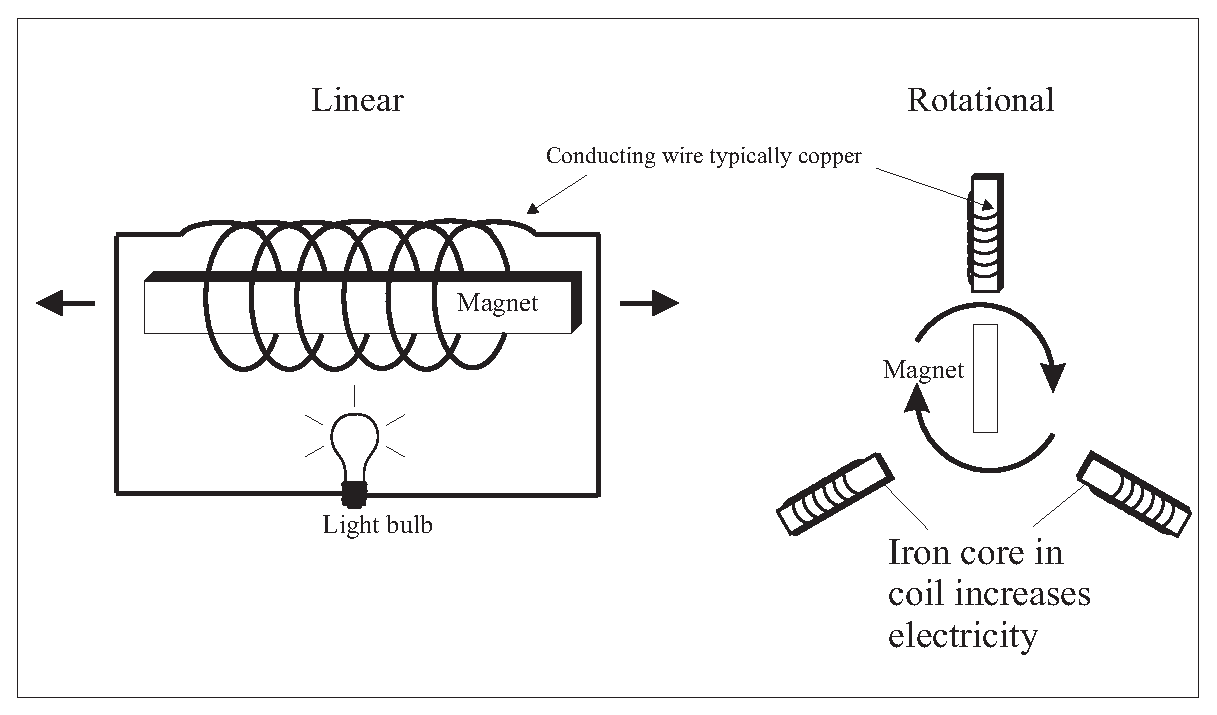
\includegraphics[scale=0.4]{../../epsimages/1ElectricityGeneration.eps}
\end{figure}

Most power stations produce steam through heat (nuclear reaction or burning fossil fuels), the steam drives a turbine which moves a magnet relative to a coil (the generator - like the above but on a much larger scale i.e. bigger magnets, bigger coils, etc), which produces electricity that is transmitted via a power network to our homes. Gas fired plants burn gas directly in a gas turbine to produce the same desired relative motion between permanent magnet and coil.

\begin{figure}[H]
\centering
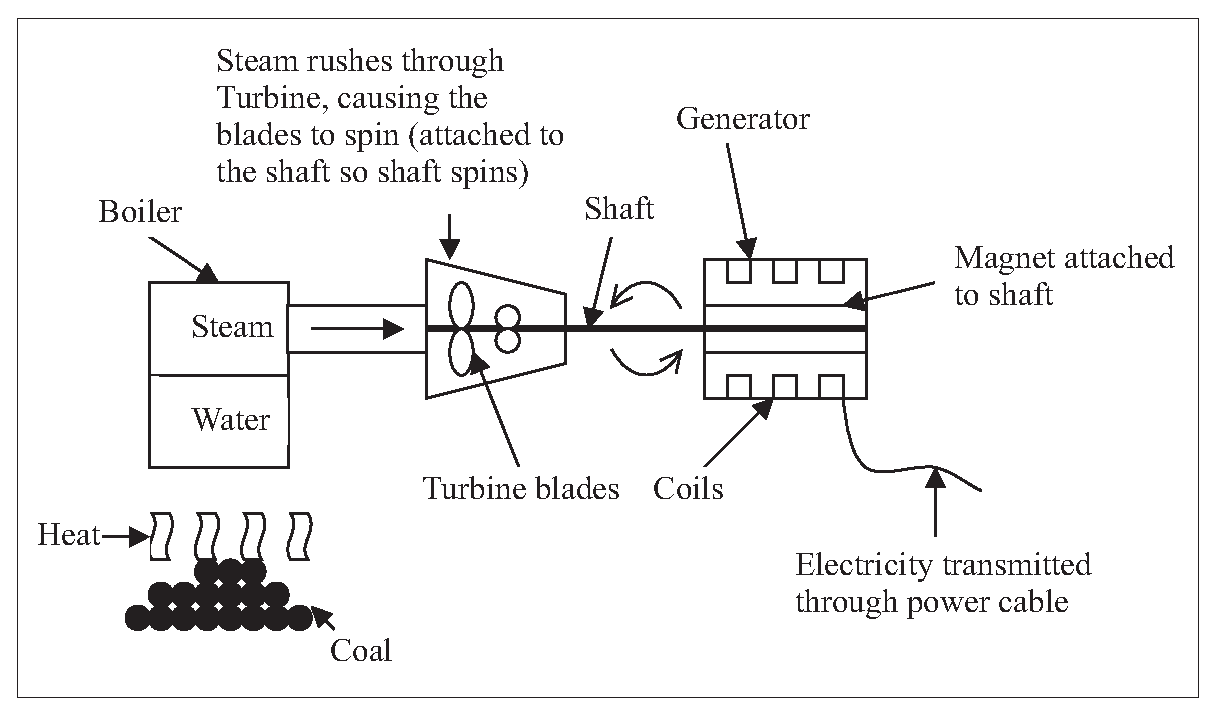
\includegraphics[scale=0.4]{../../epsimages/2SteamPower.eps}
\end{figure}

\begin{figure}[H]
\centering
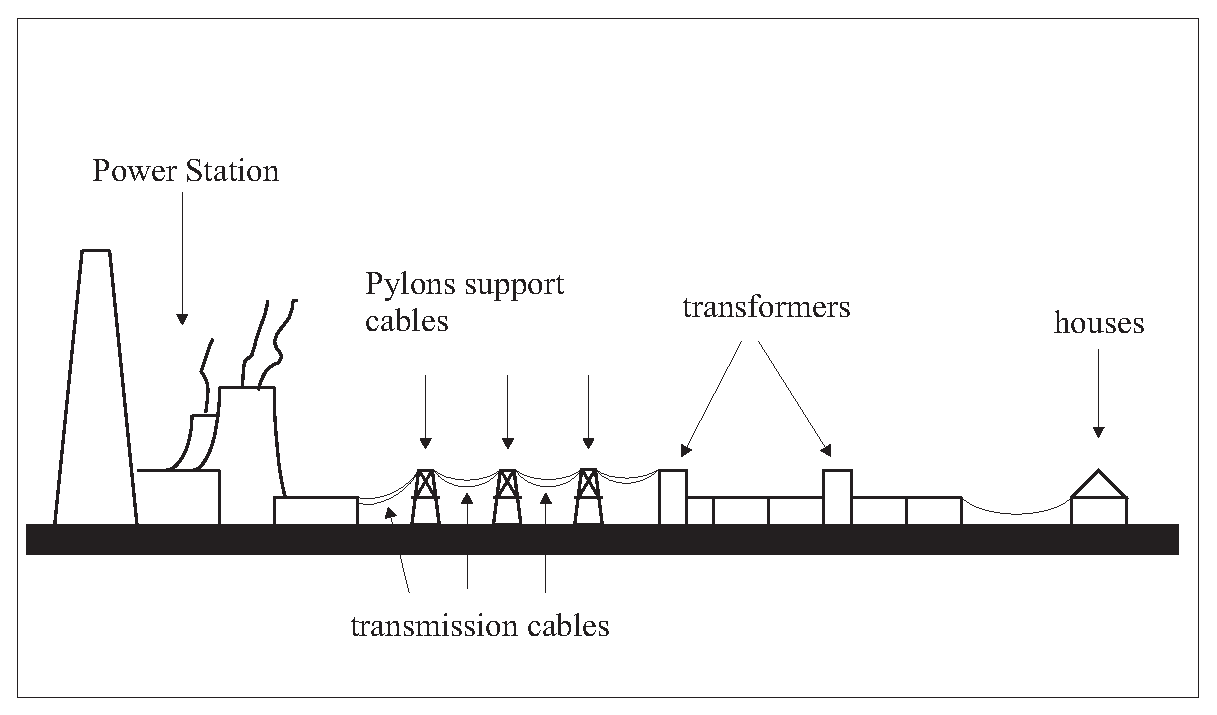
\includegraphics[scale=0.4]{../../epsimages/3PowerStation.eps}
\end{figure}

Coal, oil and gas are fossil fuels. Fossil fuels were created by
decomposing organic (plant and animal) matter a long, long time ago
and are typically found underground. Different temperatures and
pressures resulted in the organic matter transforming into coal, oil
or gas.

Why the fuss about fossil fuels?
\begin{enumerate}
\item Fossil fuel power is bad news in
the long run. It pollutes and contributes to the greenhouse effect
(global warming resulting in melting polar ice caps, floods,
droughts, disease, etc).
\item It's not going to last forever.
\item Nuclear power is 'cleaner' in terms of emissions but there's no proven way
of disposing of the nuclear waste. Oh, and it won't last forever
either!
\end{enumerate}

Renewable Energy As the name suggests renewable energy lasts
'forever'. Solar (sun), wind, geothermal, wave, hydro and biomass
(organic) are all sources of energy that will last until the sun
eventually explodes many millions of years from now. Hopefully the
human race will have moved from the earth by then! Generally the
principal of renewable electricity generation is similar to fossil
fuel electricity generation in that electricity is generated by
moving a magnet relative to a conducting coil. What is different is
the way energy is supplied to cause that motion.

The below are a few different types of available renewable energy
technologies.

\subsection*{Solar}

There are different types of solar electricity technologies, the
main ones being solar thermal and photovoltaic.

\begin{figure}[H]
\centering
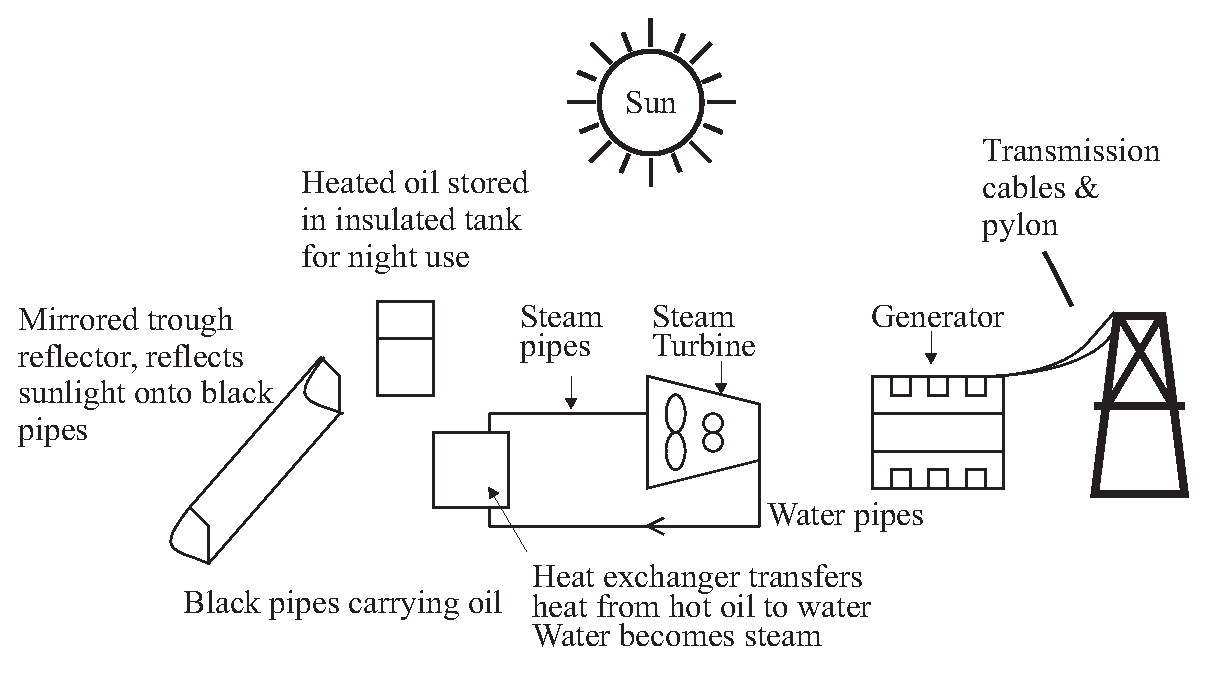
\includegraphics[scale=0.4]{../../epsimages/4solar1.eps}
\end{figure}

Solar thermal uses the heat of the sun to produce electricity. Sun
is concentrated using mirrors. This heat either creates steam which
drives a turbine which in turn drives a generator (as per fossil
fuel generation), or drives an air engine (engine that uses
expanding air to obtain motion) that drives a generator.

Photovoltaic panels convert sunlight directly into electricity. The
benefit of photovoltaic panels is that there are no moving parts,
and is therefore relatively maintenance free. The downside is that
it's very expensive at this stage (17/06/2004).

\begin{figure}[H]
\centering
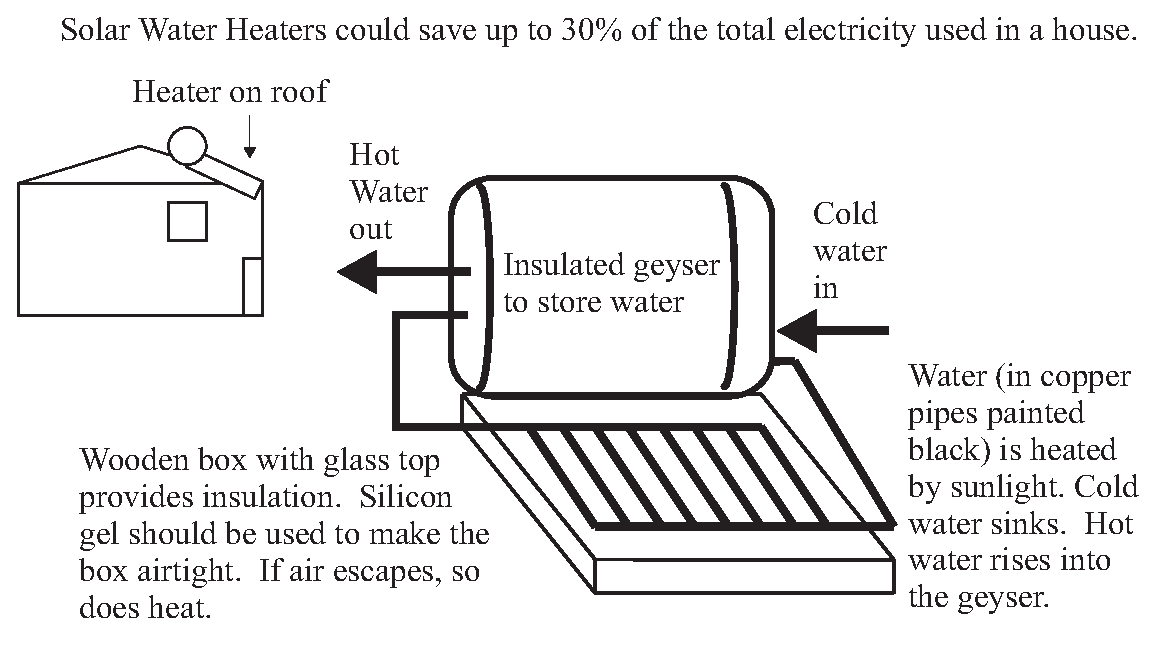
\includegraphics[scale=0.4]{../../epsimages/4solar2.eps}
\end{figure}

\subsection*{Wind}

Wind turbines catch wind that spins the blades. The blades are
connected to a shaft that spins because of the wind. This spinning
shaft spins another shaft that turns a permanent magnet relative to
conducting coils.

Note that 'gears' are used to convert the slow spinning of the 1st
shaft to a faster spin on the 2nd shaft. The generator shaft needs
to spin at the correct speed to produce the right amount and quality
of electricity. Some generators are now being modified to run at
slower speeds. This saves money as gears are not needed.

\begin{figure}[H]
\centering
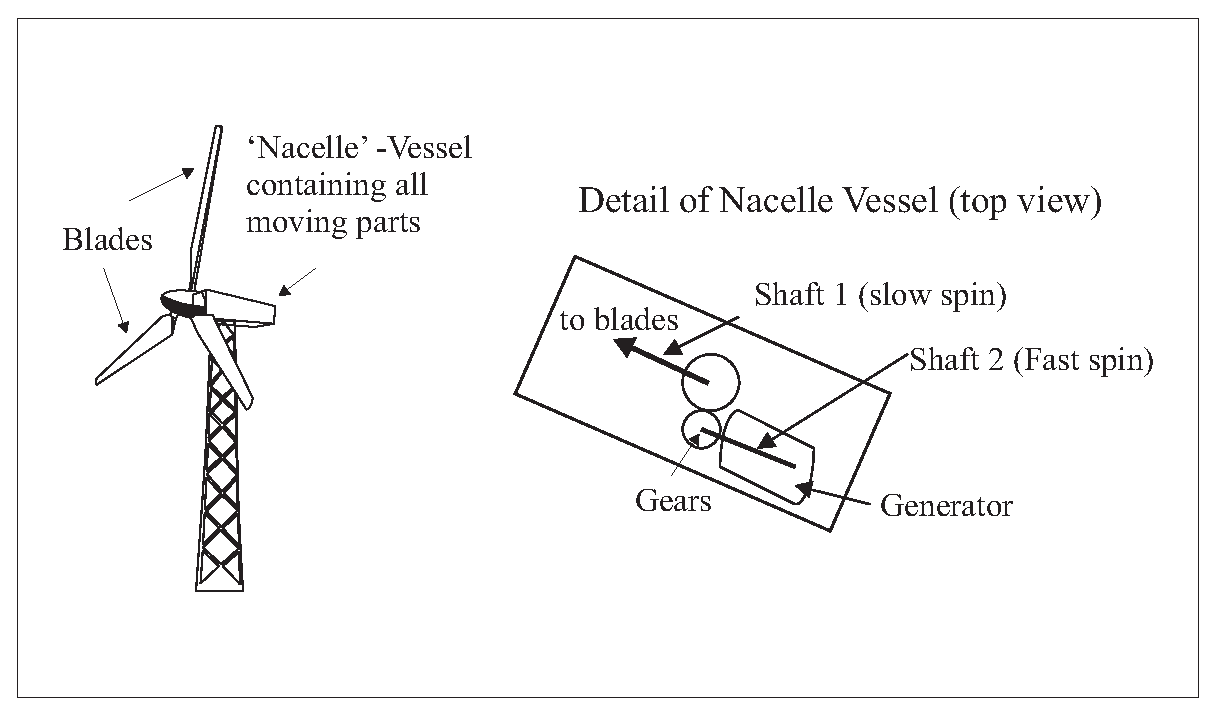
\includegraphics[scale=0.4]{../../epsimages/5Windturbine.eps}
\end{figure}

\subsection*{Biomass}

Biomass is anything organic i.e. plant or animal matter. It can be
used in the place of coal as per a normal coal fired plant and is
renewable as long as the biomass e.g. wood; is handled in a
sustainable manner. By sustainable I mean that suitable farming
practices are used so that the land is not 'over farmed' which will
result in the soil becoming barren and nothing growing there again.

\begin{figure}[H]
\centering
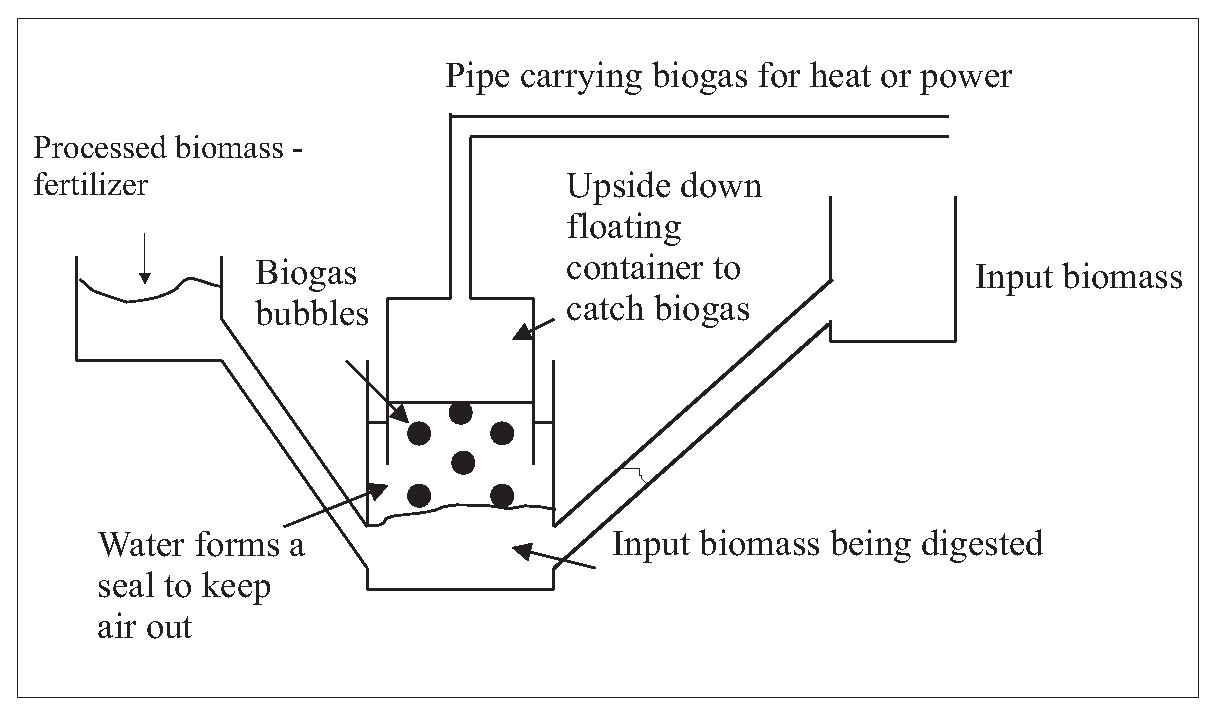
\includegraphics[scale=0.4]{../../epsimages/6biogas.eps}
\end{figure}

Biomass can also be processed using 'anaerobic digestion' to produce a gas that can be burned for heat or electricity. This 'biogas' is made up of a number of other gases that are similar to those found in fossil fuel natural gas - Except the amount of the gases are different. E.g. Natural gas has about 94% methane and biogas has about 60% methane. (Methane is a gas that can be burnt for heat or power)

Anaerobic digestion: 'Anaerobic' means 'No air'. Therefore
'anaerobic digestion' means to digest in the absence of air.
Bacteria that naturally exist in organic matter will convert organic
matter to biogas and fertilizer when all the air is removed.

Thousands of anaerobic digesters have been installed in rural India,
Nepal and China in rural area's where cow dung, human waste and
chicken litter (faeces) are all processed using anaerobic digestion
to produce gas that can be burned in the home for cooking and
heating. The leftover is used as fertilizer.

\subsection*{Geothermal Energy}

In some places on earth, the earth's crust is thinner than others.
As a result the heat from the earth's core escapes. The heat can be
captured by converting water to steam, and using the steam to drive
a steam generator as discussed above.

Hydroelectric power Water from a river is diverted to turn a water
turbine to create electricity similar to the principles of steam
generation. The water is returned to the river after driving the
turbine.

\begin{figure}[H]
\centering
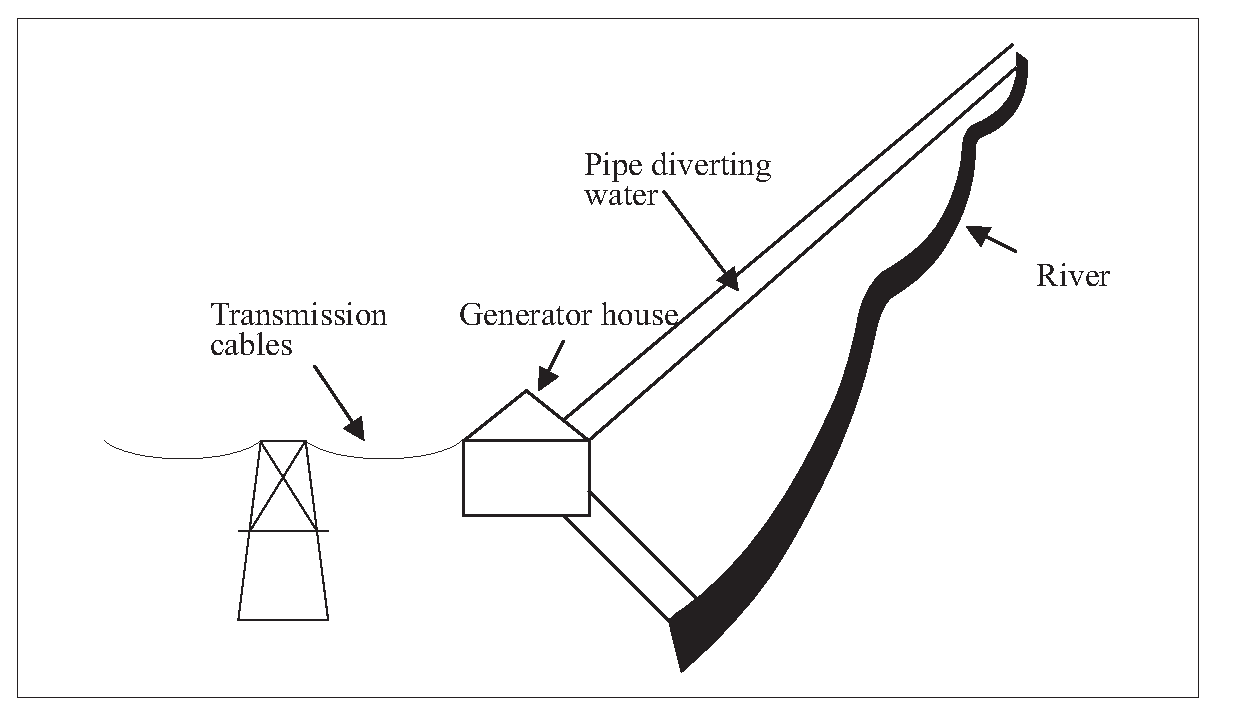
\includegraphics[scale=0.4]{../../epsimages/7hydroelectricriver.eps}
\end{figure}

\subsection*{Wave Energy}

Some wave energy generators work similarly to
wind turbines except that underwater ocean currents turns the blades
instead of wind; and of course most of the structure is under water!
\begin{figure}[H]
\centering
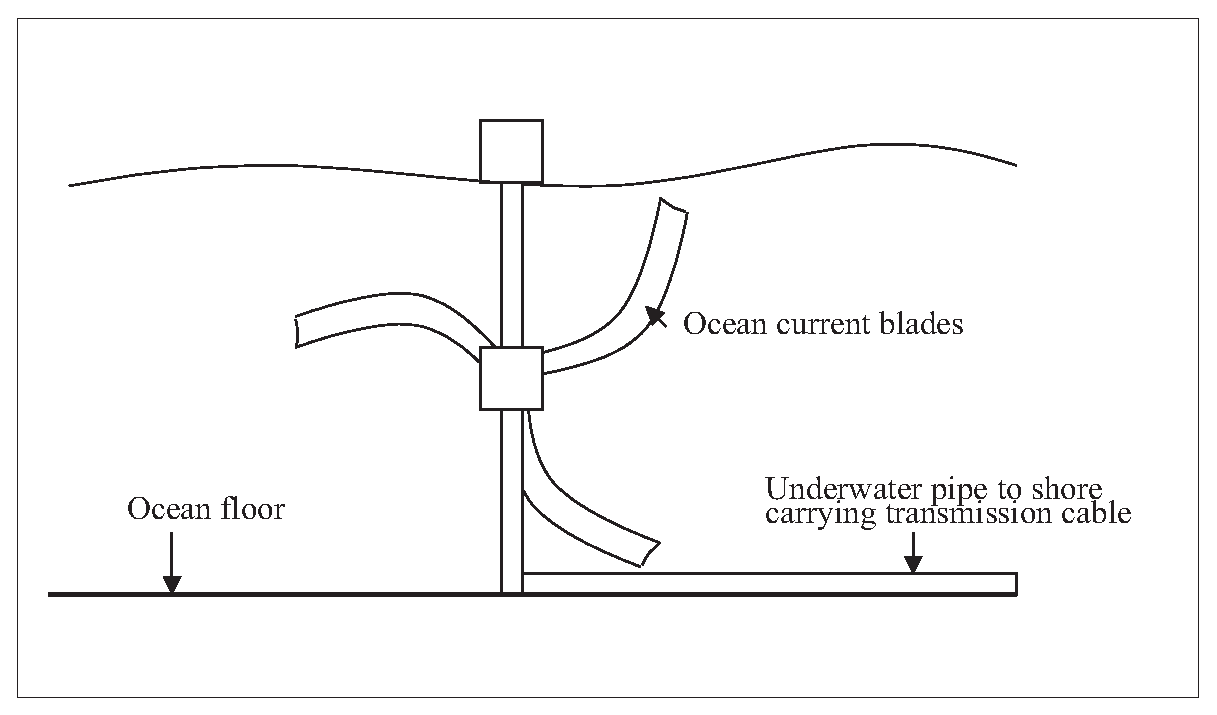
\includegraphics[scale=0.4]{../../epsimages/8hydroelectricocean1.eps}
\end{figure}

Another concept uses the rising and falling of the tides to suck air
in using a 'one way valve'. As a result air becomes compressed in a
chamber and the compressed air is let out to drive a turbine which
in turn drives a generator

\begin{figure}[H]
\centering
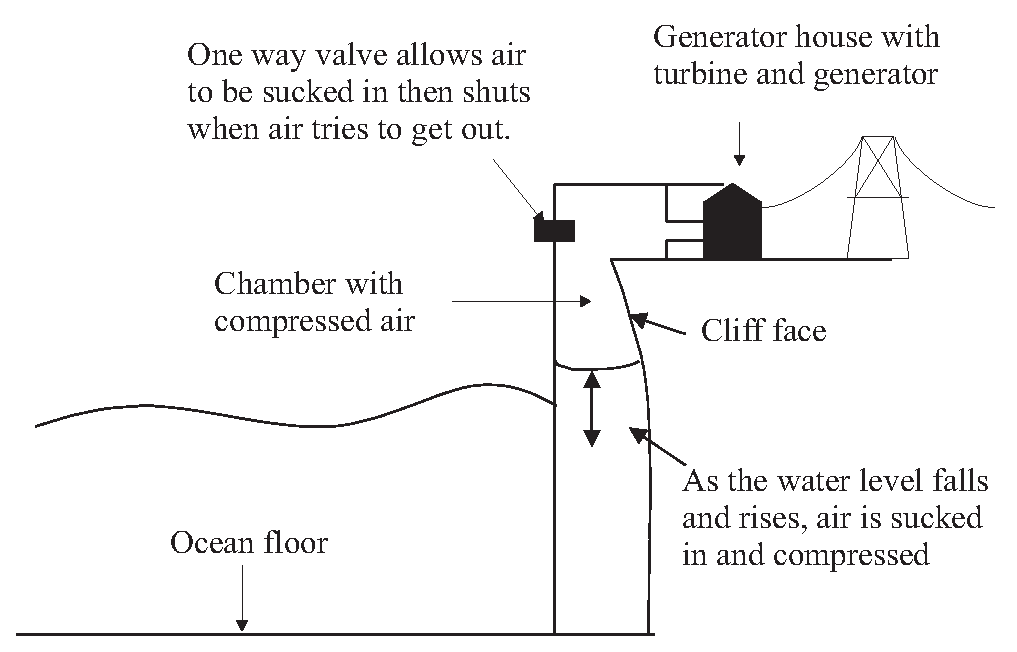
\includegraphics[scale=0.4]{../../epsimages/8hydroelectricocean2.eps}
\end{figure}

These are relatively new technologies.

Liquid Fuels Liquid fuels are used mainly for transportation. Petrol
and diesel are the most common liquid fuels and are obtained from
oil.

Sasol is the only company in the world that makes liquid fuels from
coal; and will be one of the leading companies in the world to make
liquid fuels from natural gas! The Sasol petro-chemical plants are
based in Sasolburg on the border of the Free State and in Secunda in
Mpumalanga.

However, as discussed above coal, gas and oil are fossil fuels and
are not renewable. Petrol and diesel are obtained from fossil fuels
and therefore pollute and contribute to the green house effect
(global warming).

\subsection*{Alternatives}

\subsubsection*{Biodiesel} Oil can be extracted from plants such as the
soya bean, sunflower and rapeseed by pressing it through a filter.
This oil if mixed correctly with either methanol or dry ethanol and
Sodium Hydroxide will separate the plant oil into biodiesel,
glycerol and fertilizer.

The biodiesel can be used as produced in a conventional diesel
engine with little or no modifications required.

The glycerol can be refined a bit further for pharmaceutical
companies to use, or can be used to make soap.

\subsubsection*{Ethanol}

Corn, maize and sugar cane can be used to make ethanol as a fuel
substitute for petrol. It's made by the same fermentation process
used to make alcohol. Enzymes are often used to speed up the
process.

In ethanol from sugar cane production, the leftover 'bagasse' (the
fibre part of the sugar cane) can be burned in a biomass power
station to produce electricity.

\subsubsection*{Hydrogen} Through the process of 'electrolysis'
electricity (hopefully clean, renewable electricity!) can split
water into hydrogen and oxygen. The stored hydrogen can be used in a
'fuel cell' to create electricity in a process that is opposite to
electrolysis; to drive electric motors in a car. The hydrogen can also be burned directly in a modified internal combustion engine. In both cases the 'waste' product is water.



% CHILD SECTION END 



% CHILD SECTION START 


  \chapter{Essay: How a cell phone works}

% CHILD SECTION END 



% CHILD SECTION START 


  \chapter{Essay: How a Physiotherapist uses the Concept of Levers}



% CHILD SECTION END 



% CHILD SECTION START 


  \chapter{Essay: How a Pilot Uses Vectors}

% CHILD SECTION END 



% CHILD SECTION START 

How an air traffic controller uses radar

% CHILD SECTION END 



% CHILD SECTION START 

How sonar is used for fishing

% CHILD SECTION END 



% CHILD SECTION START 

\essayauthorblurb[Asogan Moodaly received his Bachelor of Science
degree (with honours) in Mechanical Engineering from the University
of Natal, Durban in South Africa. For his final year design project
he worked on a 3-axis filament winding machine for composite (Glass
re-enforced plastic in this case) piping. He worked in Vereeniging,
Gauteng at Mine Support Products (a subsidiary of Dorbyl Heavy
Engineering) as the design engineer once he graduated. He currently
lives in the Vaal Triangle area and is working for Sasol Technology
Engineering as a mechanical engineer, ensuring the safety and
integrity of equipment installed during projects.]

\essaytitle[Pressure and Forces]

In the mining industry, the roof (hangingwall) tends to drop as the
face of the tunnel (stope) is excavated for rock containing gold.

As one can imagine, a roof falling on one's head is not a nice
prospect! Therefore the roof needs to be supported.
\begin{figure}[H]
\centering
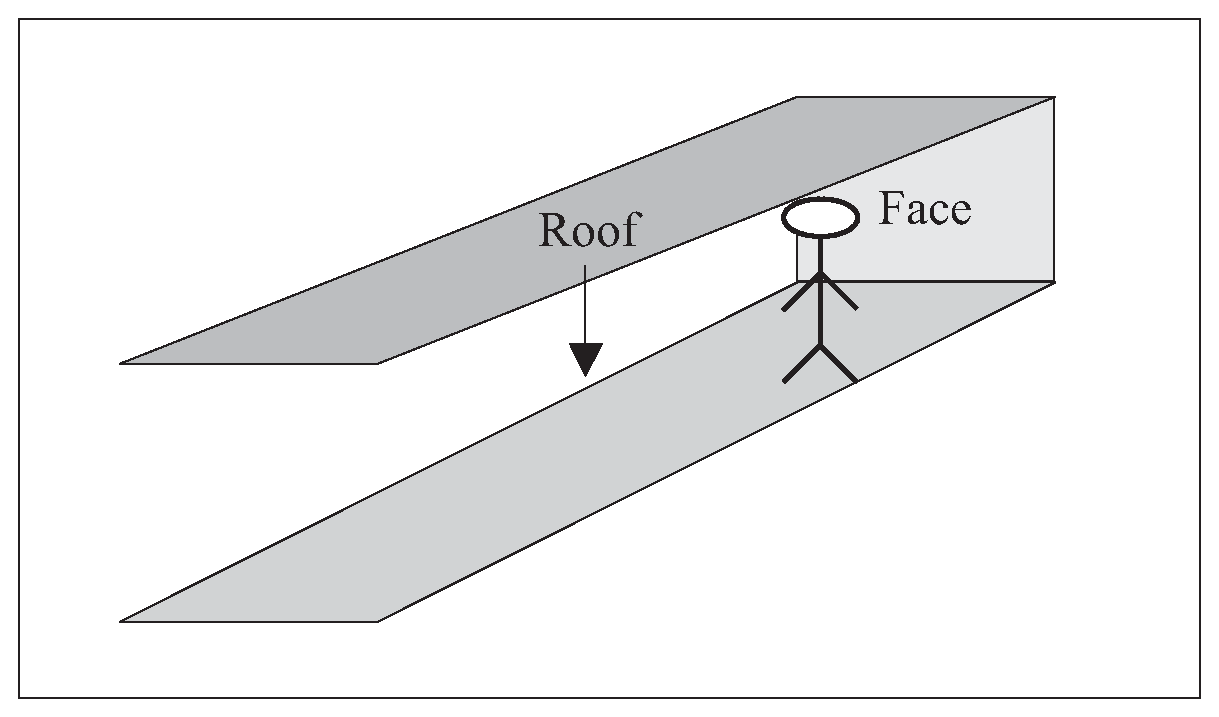
\includegraphics[scale=0.4]{../../epsimages/EssayPressure1.eps}
\end{figure}

The roof is not one big uniform chunk of rock. Rather it is broken
up into smaller chunks. It is assumed that the biggest chunk of rock
in the roof has a mass of less than 20 000 kgs therefore each
support has to be designed to resist a force related to that mass.
The strength of the material (either wood or steel) making up the
support is taken into account when working out the minimum required
size and thickness of the parts to withstand the force of the roof.

\begin{figure}[H]
\centering
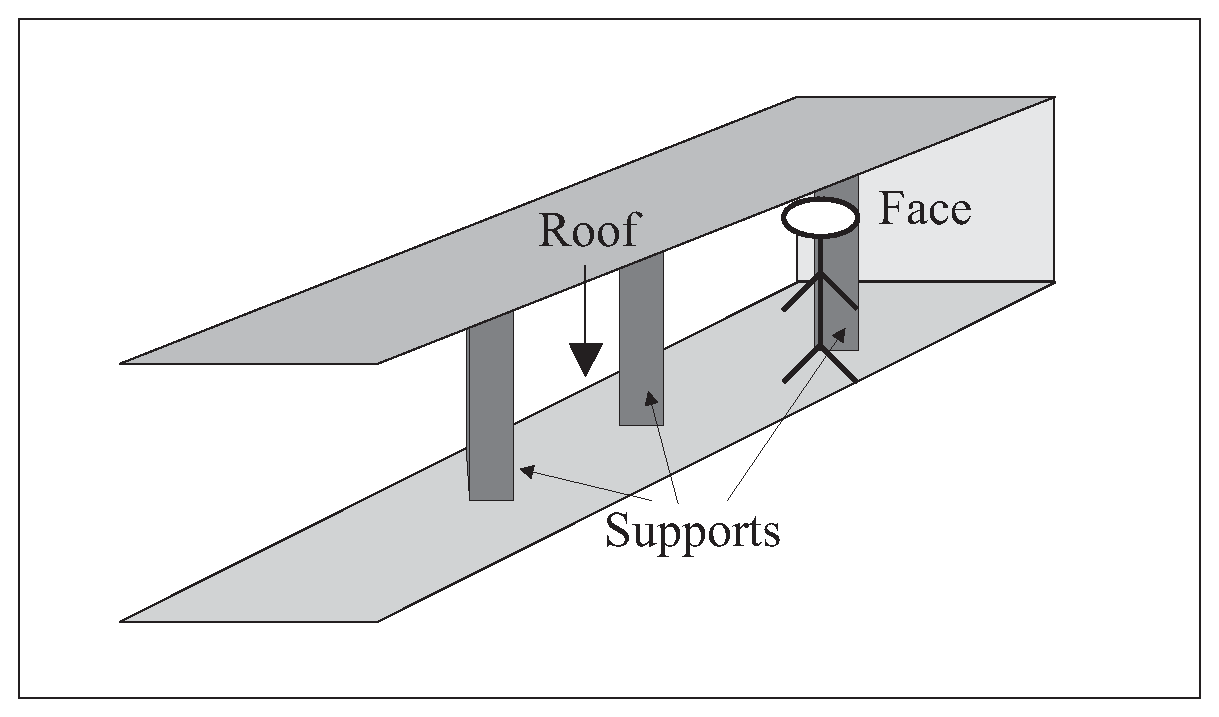
\includegraphics[scale=0.4]{../../epsimages/EssayPressure2.eps}
\end{figure}


Sometimes the design of the support is such that the support needs
to withstand the rock mass without the force breaking the roof..

Therefore hydraulic supports (hydro = water) use the principles of
force and pressure such that as a force is exerted on the support,
the water pressure increases. A pressure relief valve then squirts
out water when the pressure (and thus the force) gets too large.
Imagine a very large, modified doctor's syringe.
\begin{figure}[H]
\centering
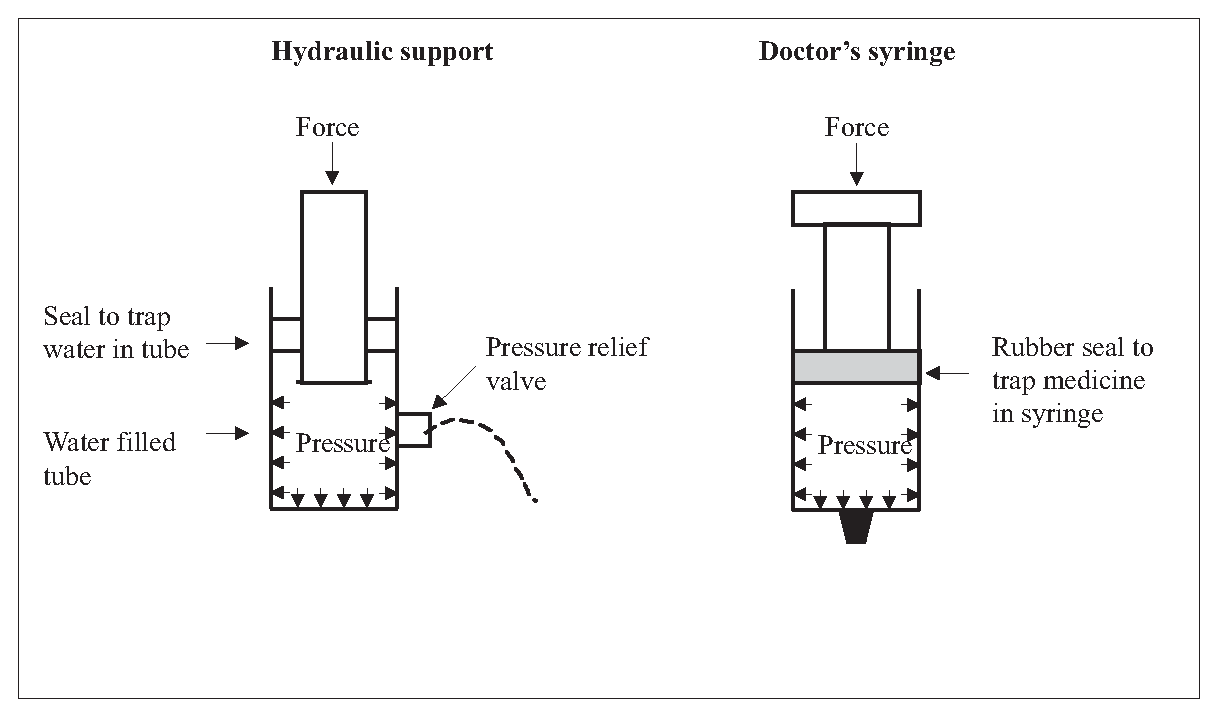
\includegraphics[scale=0.4]{../../epsimages/EssayPressure3.eps}
\end{figure}

In the petrochemical industry, there are many vessels and pipes that
are under high pressures. A vessel is a containment unit (Imagine a
pot without handles, that has the lid welded to the pot  that would
be a small vessel) where chemicals mix and react to form other
chemicals, amongst other uses.
\begin{figure}[H]
\centering
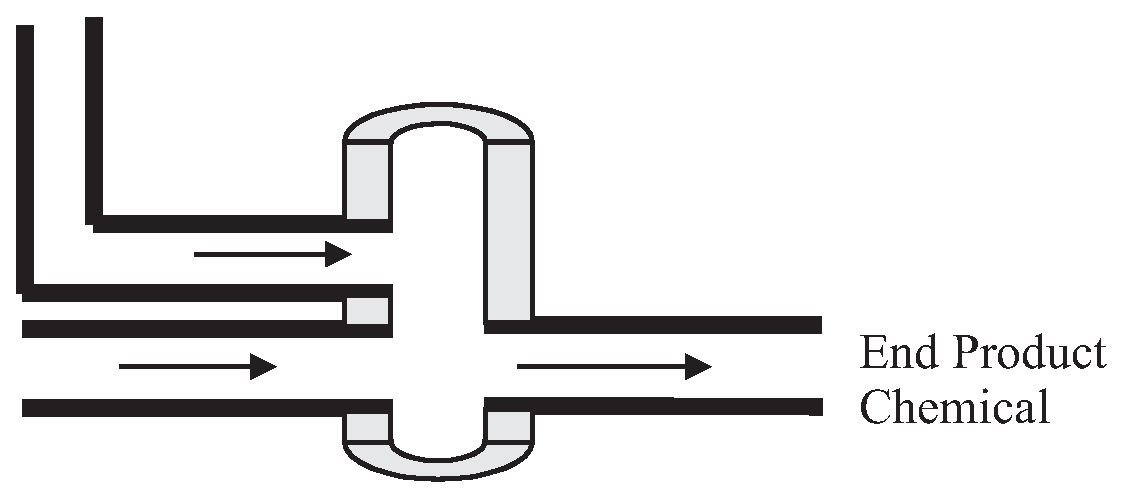
\includegraphics[scale=0.4]{../../epsimages/EssayPressure4.eps}
\end{figure}

The end product chemicals are sold to companies that use these
chemicals to make shampoo, dishwashing liquid, plastic containers,
fertilizer, etc. Anyway, some of these chemical reactions require
high temperatures and pressures in order to work. These pressures
result in forces being applied to the insides of the vessels and
pipes. Therefore the minimum thickness of the pipe and vessels walls
must be determined using calculations, to withstand these forces.
These calculations take into account the strength of the material
(typically steel, plastic or composite), the diameter and of course
the pressure inside the equipment. Let examine the concepts of
force and pressure in further detail.



\appendix
\chapter{GNU Free Documentation License}\label{fdl}

Version 1.2, November 2002 \\
Copyright \copyright\ 2000,2001,2002  Free Software Foundation, Inc.\\
59 Temple Place, Suite 330, Boston, MA  02111-1307  USA\\
Everyone is permitted to copy and distribute verbatim copies
of this license document, but changing it is not allowed.

\section*{PREAMBLE}

The purpose of this License is to make a manual, textbook, or other
functional and useful document ``free'' in the sense of freedom: to
assure everyone the effective freedom to copy and redistribute it,
with or without modifying it, either commercially or non-commercially.
Secondarily, this License preserves for the author and publisher a way
to get credit for their work, while not being considered responsible
for modifications made by others.

This License is a kind of ``copyleft'', which means that derivative
works of the document must themselves be free in the same sense.  It
complements the GNU General Public License, which is a copyleft
license designed for free software.

We have designed this License in order to use it for manuals for free
software, because free software needs free documentation: a free
program should come with manuals providing the same freedoms that the
software does.  But this License is not limited to software manuals;
it can be used for any textual work, regardless of subject matter or
whether it is published as a printed book.  We recommend this License
principally for works whose purpose is instruction or reference.


\section*{APPLICABILITY AND DEFINITIONS}
\label{applicability}

This License applies to any manual or other work, in any medium, that
contains a notice placed by the copyright holder saying it can be
distributed under the terms of this License.  Such a notice grants a
world-wide, royalty-free license, unlimited in duration, to use that
work under the conditions stated herein.  The ``Document'', below,
refers to any such manual or work.  Any member of the public is a
licensee, and is addressed as ``you''.  You accept the license if you
copy, modify or distribute the work in a way requiring permission
under copyright law.

A ``Modified Version'' of the Document means any work containing the
Document or a portion of it, either copied verbatim, or with
modifications and/or translated into another language.

A ``Secondary Section'' is a named appendix or a front-matter section of
the Document that deals exclusively with the relationship of the
publishers or authors of the Document to the Document's overall subject
(or to related matters) and contains nothing that could fall directly
within that overall subject.  (Thus, if the Document is in part a
textbook of mathematics, a Secondary Section may not explain any
mathematics.)  The relationship could be a matter of historical
connection with the subject or with related matters, or of legal,
commercial, philosophical, ethical or political position regarding
them.

The ``Invariant Sections'' are certain Secondary Sections whose titles
are designated, as being those of Invariant Sections, in the notice
that says that the Document is released under this License.  If a
section does not fit the above definition of Secondary then it is not
allowed to be designated as Invariant.  The Document may contain zero
Invariant Sections.  If the Document does not identify any Invariant
Sections then there are none.

The ``Cover Texts'' are certain short passages of text that are listed,
as Front-Cover Texts or Back-Cover Texts, in the notice that says that
the Document is released under this License.  A Front-Cover Text may
be at most 5 words, and a Back-Cover Text may be at most 25 words.

A ``Transparent'' copy of the Document means a machine-readable copy,
represented in a format whose specification is available to the
general public, that is suitable for revising the document
straightforwardly with generic text editors or (for images composed of
pixels) generic paint programs or (for drawings) some widely available
drawing editor, and that is suitable for input to text formatters or
for automatic translation to a variety of formats suitable for input
to text formatters.  A copy made in an otherwise Transparent file
format whose markup, or absence of markup, has been arranged to thwart
or discourage subsequent modification by readers is not Transparent.
An image format is not Transparent if used for any substantial amount
of text.  A copy that is not ``Transparent'' is called ``Opaque''.

Examples of suitable formats for Transparent copies include plain
ASCII without markup, Texinfo input format, \LaTeX\ input format, SGML
or XML using a publicly available DTD and standard-conforming simple
HTML, PostScript or PDF designed for human modification. Examples of
transparent image formats include PNG, XCF and JPG. Opaque formats
include proprietary formats that can be read and edited only by
proprietary word processors, SGML or XML for which the DTD and/or
processing tools are not generally available, and the
machine-generated HTML, PostScript or PDF produced by some word
processors for output purposes only.

The ``Title Page'' means, for a printed book, the title page itself,
plus such following pages as are needed to hold, legibly, the material
this License requires to appear in the title page.  For works in
formats which do not have any title page as such, ``Title Page'' means
the text near the most prominent appearance of the work's title,
preceding the beginning of the body of the text.

A section ``Entitled XYZ'' means a named subunit of the Document whose
title either is precisely XYZ or contains XYZ in parentheses following
text that translates XYZ in another language.  (Here XYZ stands for a
specific section name mentioned below, such as ``Acknowledgements'',
``Dedications'', ``Endorsements'', or ``History''.)  To ``Preserve the Title''
of such a section when you modify the Document means that it remains a
section ``Entitled XYZ'' according to this definition.

The Document may include Warranty Disclaimers next to the notice which
states that this License applies to the Document.  These Warranty
Disclaimers are considered to be included by reference in this
License, but only as regards disclaiming warranties: any other
implication that these Warranty Disclaimers may have is void and has
no effect on the meaning of this License.


\section*{VERBATIM COPYING}
\label{verbatim}

You may copy and distribute the Document in any medium, either
commercially or non-commercially, provided that this License, the
copyright notices, and the license notice saying this License applies
to the Document are reproduced in all copies, and that you add no other
conditions whatsoever to those of this License.  You may not use
technical measures to obstruct or control the reading or further
copying of the copies you make or distribute.  However, you may accept
compensation in exchange for copies.  If you distribute a large enough
number of copies you must also follow the conditions in
section~\ref{copying}.

You may also lend copies, under the same conditions stated above, and
you may publicly display copies.


\section*{COPYING IN QUANTITY}
\label{copying}

If you publish printed copies (or copies in media that commonly have
printed covers) of the Document, numbering more than 100, and the
Document's license notice requires Cover Texts, you must enclose the
copies in covers that carry, clearly and legibly, all these Cover
Texts: Front-Cover Texts on the front cover, and Back-Cover Texts on
the back cover.  Both covers must also clearly and legibly identify
you as the publisher of these copies.  The front cover must present
the full title with all words of the title equally prominent and
visible.  You may add other material on the covers in addition.
Copying with changes limited to the covers, as long as they preserve
the title of the Document and satisfy these conditions, can be treated
as verbatim copying in other respects.

If the required texts for either cover are too voluminous to fit
legibly, you should put the first ones listed (as many as fit
reasonably) on the actual cover, and continue the rest onto adjacent
pages.

If you publish or distribute Opaque copies of the Document numbering
more than 100, you must either include a machine-readable Transparent
copy along with each Opaque copy, or state in or with each Opaque copy
a computer-network location from which the general network-using
public has access to download using public-standard network protocols
a complete Transparent copy of the Document, free of added material.
If you use the latter option, you must take reasonably prudent steps,
when you begin distribution of Opaque copies in quantity, to ensure
that this Transparent copy will remain thus accessible at the stated
location until at least one year after the last time you distribute an
Opaque copy (directly or through your agents or retailers) of that
edition to the public.

It is requested, but not required, that you contact the authors of the
Document well before redistributing any large number of copies, to give
them a chance to provide you with an updated version of the Document.


\section*{MODIFICATIONS}
\label{modifications}

You may copy and distribute a Modified Version of the Document under
the conditions of sections~\ref{verbatim} and \ref{copying} above,
provided that you release
the Modified Version under precisely this License, with the Modified
Version filling the role of the Document, thus licensing distribution
and modification of the Modified Version to whoever possesses a copy
of it.  In addition, you must do these things in the Modified Version:

\begin{enumerate}
\item Use in the Title Page (and on the covers, if any) a title distinct
   from that of the Document, and from those of previous versions
   (which should, if there were any, be listed in the History section
   of the Document).  You may use the same title as a previous version
   if the original publisher of that version gives permission.
\item List on the Title Page, as authors, one or more persons or entities
   responsible for authorship of the modifications in the Modified
   Version, together with at least five of the principal authors of the
   Document (all of its principal authors, if it has fewer than five),
   unless they release you from this requirement.
\item State on the Title page the name of the publisher of the
   Modified Version, as the publisher.
\item Preserve all the copyright notices of the Document.
\item Add an appropriate copyright notice for your modifications
   adjacent to the other copyright notices.
\item Include, immediately after the copyright notices, a license notice
   giving the public permission to use the Modified Version under the
   terms of this License, in the form shown in the Addendum below.
\item Preserve in that license notice the full lists of Invariant Sections
   and required Cover Texts given in the Document's license notice.
\item Include an unaltered copy of this License.
\item Preserve the section Entitled ``History'', Preserve its Title, and add
   to it an item stating at least the title, year, new authors, and
   publisher of the Modified Version as given on the Title Page.  If
   there is no section Entitled ``History'' in the Document, create one
   stating the title, year, authors, and publisher of the Document as
   given on its Title Page, then add an item describing the Modified
   Version as stated in the previous sentence.
\item Preserve the network location, if any, given in the Document for
   public access to a Transparent copy of the Document, and likewise
   the network locations given in the Document for previous versions
   it was based on.  These may be placed in the ``History'' section.
   You may omit a network location for a work that was published at
   least four years before the Document itself, or if the original
   publisher of the version it refers to gives permission.
\item For any section Entitled ``Acknowledgements'' or ``Dedications'',
   Preserve the Title of the section, and preserve in the section all
   the substance and tone of each of the contributor acknowledgements
   and/or dedications given therein.
\item Preserve all the Invariant Sections of the Document,
   unaltered in their text and in their titles.  Section numbers
   or the equivalent are not considered part of the section titles.
\item Delete any section Entitled ``Endorsements''.  Such a section
   may not be included in the Modified Version.
\item Do not re-title any existing section to be Entitled ``Endorsements''
   or to conflict in title with any Invariant Section.
\item Preserve any Warranty Disclaimers.
\end{enumerate}

If the Modified Version includes new front-matter sections or
appendices that qualify as Secondary Sections and contain no material
copied from the Document, you may at your option designate some or all
of these sections as invariant.  To do this, add their titles to the
list of Invariant Sections in the Modified Version's license notice.
These titles must be distinct from any other section titles.

You may add a section Entitled ``Endorsements'', provided it contains
nothing but endorsements of your Modified Version by various
parties--for example, statements of peer review or that the text has
been approved by an organisation as the authoritative definition of a
standard.

You may add a passage of up to five words as a Front-Cover Text, and a
passage of up to 25 words as a Back-Cover Text, to the end of the list
of Cover Texts in the Modified Version.  Only one passage of
Front-Cover Text and one of Back-Cover Text may be added by (or
through arrangements made by) any one entity.  If the Document already
includes a cover text for the same cover, previously added by you or
by arrangement made by the same entity you are acting on behalf of,
you may not add another; but you may replace the old one, on explicit
permission from the previous publisher that added the old one.

The author(s) and publisher(s) of the Document do not by this License
give permission to use their names for publicity for or to assert or
imply endorsement of any Modified Version.


\section*{COMBINING DOCUMENTS}
\label{combining}

You may combine the Document with other documents released under this
License, under the terms defined in section~\ref{modifications}
above for modified
versions, provided that you include in the combination all of the
Invariant Sections of all of the original documents, unmodified, and
list them all as Invariant Sections of your combined work in its
license notice, and that you preserve all their Warranty Disclaimers.

The combined work need only contain one copy of this License, and
multiple identical Invariant Sections may be replaced with a single
copy.  If there are multiple Invariant Sections with the same name but
different contents, make the title of each such section unique by
adding at the end of it, in parentheses, the name of the original
author or publisher of that section if known, or else a unique number.
Make the same adjustment to the section titles in the list of
Invariant Sections in the license notice of the combined work.

In the combination, you must combine any sections Entitled ``History''
in the various original documents, forming one section Entitled
``History''; likewise combine any sections Entitled ``Acknowledgements'',
and any sections Entitled ``Dedications''.  You must delete all sections
Entitled ``Endorsements''.


\section*{COLLECTIONS OF DOCUMENTS}
\label{collections}

You may make a collection consisting of the Document and other documents
released under this License, and replace the individual copies of this
License in the various documents with a single copy that is included in
the collection, provided that you follow the rules of this License for
verbatim copying of each of the documents in all other respects.

You may extract a single document from such a collection, and distribute
it individually under this License, provided you insert a copy of this
License into the extracted document, and follow this License in all
other respects regarding verbatim copying of that document.


\section*{AGGREGATION WITH INDEPENDENT WORKS}
\label{aggregation}

A compilation of the Document or its derivatives with other separate
and independent documents or works, in or on a volume of a storage or
distribution medium, is called an ``aggregate'' if the copyright
resulting from the compilation is not used to limit the legal rights
of the compilation's users beyond what the individual works permit.
When the Document is included an aggregate, this License does not
apply to the other works in the aggregate which are not themselves
derivative works of the Document.

If the Cover Text requirement of section~\ref{copying} is applicable to
these copies of the Document, then if the Document is less than one half
of the entire aggregate, the Document's Cover Texts may be placed on
covers that bracket the Document within the aggregate, or the
electronic equivalent of covers if the Document is in electronic form.
Otherwise they must appear on printed covers that bracket the whole
aggregate.


\section*{TRANSLATION}
\label{translation}

Translation is considered a kind of modification, so you may
distribute translations of the Document under the terms of
section~\ref{modifications}.
Replacing Invariant Sections with translations requires special
permission from their copyright holders, but you may include
translations of some or all Invariant Sections in addition to the
original versions of these Invariant Sections.  You may include a
translation of this License, and all the license notices in the
Document, and any Warranty Disclaimers, provided that you also include
the original English version of this License and the original versions
of those notices and disclaimers.  In case of a disagreement between
the translation and the original version of this License or a notice
or disclaimer, the original version will prevail.

If a section in the Document is Entitled ``Acknowledgements'',
``Dedications'', or ``History'', the requirement
(section~\ref{modifications}) to Preserve
its Title (section~\ref{applicability}) will typically require
changing the actual title.


\section*{TERMINATION}
\label{termination}

You may not copy, modify, sub-license, or distribute the Document except
as expressly provided for under this License.  Any other attempt to
copy, modify, sub-license or distribute the Document is void, and will
automatically terminate your rights under this License.  However,
parties who have received copies, or rights, from you under this
License will not have their licenses terminated so long as such
parties remain in full compliance.


\section*{FUTURE REVISIONS OF THIS LICENSE}
\label{future}

The Free Software Foundation may publish new, revised versions
of the GNU Free Documentation License from time to time.  Such new
versions will be similar in spirit to the present version, but may
differ in detail to address new problems or concerns.  See
http://www.gnu.org/copyleft/.

Each version of the License is given a distinguishing version number.
If the Document specifies that a particular numbered version of this
License ``or any later version'' applies to it, you have the option of
following the terms and conditions either of that specified version or
of any later version that has been published (not as a draft) by the
Free Software Foundation.  If the Document does not specify a version
number of this License, you may choose any version ever published (not
as a draft) by the Free Software Foundation.


\section*{ADDENDUM: How to use this License for your documents}

To use this License in a document you have written, include a copy of
the License in the document and put the following copyright and
license notices just after the title page:

\begin{quote}
    Copyright \copyright\ YEAR  YOUR NAME.
    Permission is granted to copy, distribute and/or modify this document
    under the terms of the GNU Free Documentation License, Version 1.2
    or any later version published by the Free Software Foundation;
    with no Invariant Sections, no Front-Cover Texts, and no Back-Cover Texts.
    A copy of the license is included in the section entitled ``GNU
    Free Documentation License''.
\end{quote}

If you have Invariant Sections, Front-Cover Texts and Back-Cover Texts,
replace the ``with...Texts.'' line with this:

    with the Invariant Sections being LIST THEIR TITLES, with the
    Front-Cover Texts being LIST, and with the Back-Cover Texts being LIST.

If you have Invariant Sections without Cover Texts, or some other
combination of the three, merge those two alternatives to suit the
situation.

If your document contains nontrivial examples of program code, we
recommend releasing these examples in parallel under your choice of
free software license, such as the GNU General Public License,
to permit their use in free software.




\end{document}
